\documentclass[twoside]{book}

% Packages required by doxygen
\usepackage{calc}
\usepackage{doxygen}
\usepackage{graphicx}
\usepackage[utf8]{inputenc}
\usepackage{makeidx}
\usepackage{multicol}
\usepackage{multirow}
\usepackage{fixltx2e}
\PassOptionsToPackage{warn}{textcomp}
\usepackage{textcomp}
\usepackage[nointegrals]{wasysym}
\usepackage[table]{xcolor}

% Font selection
\usepackage[T1]{fontenc}
\usepackage{mathptmx}
\usepackage[scaled=.90]{helvet}
\usepackage{courier}
\usepackage{amssymb}
\usepackage{sectsty}
\renewcommand{\familydefault}{\sfdefault}
\allsectionsfont{%
  \fontseries{bc}\selectfont%
  \color{darkgray}%
}
\renewcommand{\DoxyLabelFont}{%
  \fontseries{bc}\selectfont%
  \color{darkgray}%
}
\newcommand{\+}{\discretionary{\mbox{\scriptsize$\hookleftarrow$}}{}{}}

% Page & text layout
\usepackage{geometry}
\geometry{%
  a4paper,%
  top=2.5cm,%
  bottom=2.5cm,%
  left=2.5cm,%
  right=2.5cm%
}
\tolerance=750
\hfuzz=15pt
\hbadness=750
\setlength{\emergencystretch}{15pt}
\setlength{\parindent}{0cm}
\setlength{\parskip}{0.2cm}
\makeatletter
\renewcommand{\paragraph}{%
  \@startsection{paragraph}{4}{0ex}{-1.0ex}{1.0ex}{%
    \normalfont\normalsize\bfseries\SS@parafont%
  }%
}
\renewcommand{\subparagraph}{%
  \@startsection{subparagraph}{5}{0ex}{-1.0ex}{1.0ex}{%
    \normalfont\normalsize\bfseries\SS@subparafont%
  }%
}
\makeatother

% Headers & footers
\usepackage{fancyhdr}
\pagestyle{fancyplain}
\fancyhead[LE]{\fancyplain{}{\bfseries\thepage}}
\fancyhead[CE]{\fancyplain{}{}}
\fancyhead[RE]{\fancyplain{}{\bfseries\leftmark}}
\fancyhead[LO]{\fancyplain{}{\bfseries\rightmark}}
\fancyhead[CO]{\fancyplain{}{}}
\fancyhead[RO]{\fancyplain{}{\bfseries\thepage}}
\fancyfoot[LE]{\fancyplain{}{}}
\fancyfoot[CE]{\fancyplain{}{}}
\fancyfoot[RE]{\fancyplain{}{\bfseries\scriptsize Generated on Fri Oct 3 2014 17\+:23\+:02 for L\+M\+F library by Doxygen }}
\fancyfoot[LO]{\fancyplain{}{\bfseries\scriptsize Generated on Fri Oct 3 2014 17\+:23\+:02 for L\+M\+F library by Doxygen }}
\fancyfoot[CO]{\fancyplain{}{}}
\fancyfoot[RO]{\fancyplain{}{}}
\renewcommand{\footrulewidth}{0.4pt}
\renewcommand{\chaptermark}[1]{%
  \markboth{#1}{}%
}
\renewcommand{\sectionmark}[1]{%
  \markright{\thesection\ #1}%
}

% Indices & bibliography
\usepackage{natbib}
\usepackage[titles]{tocloft}
\setcounter{tocdepth}{3}
\setcounter{secnumdepth}{5}
\makeindex

% Hyperlinks (required, but should be loaded last)
\usepackage{ifpdf}
\ifpdf
  \usepackage[pdftex,pagebackref=true]{hyperref}
\else
  \usepackage[ps2pdf,pagebackref=true]{hyperref}
\fi
\hypersetup{%
  colorlinks=true,%
  linkcolor=blue,%
  citecolor=blue,%
  unicode%
}

% Custom commands
\newcommand{\clearemptydoublepage}{%
  \newpage{\pagestyle{empty}\cleardoublepage}%
}


%===== C O N T E N T S =====

\begin{document}

% Titlepage & ToC
\hypersetup{pageanchor=false,
             bookmarks=true,
             bookmarksnumbered=true,
             pdfencoding=unicode
            }
\pagenumbering{roman}
\begin{titlepage}
\vspace*{7cm}
\begin{center}%
{\Large L\+M\+F library }\\
\vspace*{1cm}
{\large Generated by Doxygen 1.8.7}\\
\vspace*{0.5cm}
{\small Fri Oct 3 2014 17:23:02}\\
\end{center}
\end{titlepage}
\clearemptydoublepage
\tableofcontents
\clearemptydoublepage
\pagenumbering{arabic}
\hypersetup{pageanchor=true}

%--- Begin generated contents ---
\chapter{Namespace Index}
\section{Packages}
Here are the packages with brief descriptions (if available)\+:\begin{DoxyCompactList}
\item\contentsline{section}{\hyperlink{namespacelmf}{lmf} }{\pageref{namespacelmf}}{}
\item\contentsline{section}{\hyperlink{namespacelmf_1_1src}{lmf.\+src} }{\pageref{namespacelmf_1_1src}}{}
\item\contentsline{section}{\hyperlink{namespacelmf_1_1src_1_1common}{lmf.\+src.\+common} }{\pageref{namespacelmf_1_1src_1_1common}}{}
\item\contentsline{section}{\hyperlink{namespacelmf_1_1src_1_1common_1_1range}{lmf.\+src.\+common.\+range} }{\pageref{namespacelmf_1_1src_1_1common_1_1range}}{}
\item\contentsline{section}{\hyperlink{namespacelmf_1_1src_1_1config}{lmf.\+src.\+config} }{\pageref{namespacelmf_1_1src_1_1config}}{}
\item\contentsline{section}{\hyperlink{namespacelmf_1_1src_1_1config_1_1mdf}{lmf.\+src.\+config.\+mdf} }{\pageref{namespacelmf_1_1src_1_1config_1_1mdf}}{}
\item\contentsline{section}{\hyperlink{namespacelmf_1_1src_1_1config_1_1tex}{lmf.\+src.\+config.\+tex} }{\pageref{namespacelmf_1_1src_1_1config_1_1tex}}{}
\item\contentsline{section}{\hyperlink{namespacelmf_1_1src_1_1core}{lmf.\+src.\+core} }{\pageref{namespacelmf_1_1src_1_1core}}{}
\item\contentsline{section}{\hyperlink{namespacelmf_1_1src_1_1core_1_1definition}{lmf.\+src.\+core.\+definition} }{\pageref{namespacelmf_1_1src_1_1core_1_1definition}}{}
\item\contentsline{section}{\hyperlink{namespacelmf_1_1src_1_1core_1_1form}{lmf.\+src.\+core.\+form} }{\pageref{namespacelmf_1_1src_1_1core_1_1form}}{}
\item\contentsline{section}{\hyperlink{namespacelmf_1_1src_1_1core_1_1form__representation}{lmf.\+src.\+core.\+form\+\_\+representation} }{\pageref{namespacelmf_1_1src_1_1core_1_1form__representation}}{}
\item\contentsline{section}{\hyperlink{namespacelmf_1_1src_1_1core_1_1global__information}{lmf.\+src.\+core.\+global\+\_\+information} }{\pageref{namespacelmf_1_1src_1_1core_1_1global__information}}{}
\item\contentsline{section}{\hyperlink{namespacelmf_1_1src_1_1core_1_1lexical__entry}{lmf.\+src.\+core.\+lexical\+\_\+entry} }{\pageref{namespacelmf_1_1src_1_1core_1_1lexical__entry}}{}
\item\contentsline{section}{\hyperlink{namespacelmf_1_1src_1_1core_1_1lexical__resource}{lmf.\+src.\+core.\+lexical\+\_\+resource} }{\pageref{namespacelmf_1_1src_1_1core_1_1lexical__resource}}{}
\item\contentsline{section}{\hyperlink{namespacelmf_1_1src_1_1core_1_1lexicon}{lmf.\+src.\+core.\+lexicon} }{\pageref{namespacelmf_1_1src_1_1core_1_1lexicon}}{}
\item\contentsline{section}{\hyperlink{namespacelmf_1_1src_1_1core_1_1representation}{lmf.\+src.\+core.\+representation} }{\pageref{namespacelmf_1_1src_1_1core_1_1representation}}{}
\item\contentsline{section}{\hyperlink{namespacelmf_1_1src_1_1core_1_1sense}{lmf.\+src.\+core.\+sense} }{\pageref{namespacelmf_1_1src_1_1core_1_1sense}}{}
\item\contentsline{section}{\hyperlink{namespacelmf_1_1src_1_1core_1_1statement}{lmf.\+src.\+core.\+statement} }{\pageref{namespacelmf_1_1src_1_1core_1_1statement}}{}
\item\contentsline{section}{\hyperlink{namespacelmf_1_1src_1_1core_1_1text__representation}{lmf.\+src.\+core.\+text\+\_\+representation} }{\pageref{namespacelmf_1_1src_1_1core_1_1text__representation}}{}
\item\contentsline{section}{\hyperlink{namespacelmf_1_1src_1_1input}{lmf.\+src.\+input} }{\pageref{namespacelmf_1_1src_1_1input}}{}
\item\contentsline{section}{\hyperlink{namespacelmf_1_1src_1_1input_1_1elan}{lmf.\+src.\+input.\+elan} }{\pageref{namespacelmf_1_1src_1_1input_1_1elan}}{}
\item\contentsline{section}{\hyperlink{namespacelmf_1_1src_1_1input_1_1ite}{lmf.\+src.\+input.\+ite} }{\pageref{namespacelmf_1_1src_1_1input_1_1ite}}{}
\item\contentsline{section}{\hyperlink{namespacelmf_1_1src_1_1input_1_1mdf}{lmf.\+src.\+input.\+mdf} }{\pageref{namespacelmf_1_1src_1_1input_1_1mdf}}{}
\item\contentsline{section}{\hyperlink{namespacelmf_1_1src_1_1input_1_1toolbox__settings}{lmf.\+src.\+input.\+toolbox\+\_\+settings} }{\pageref{namespacelmf_1_1src_1_1input_1_1toolbox__settings}}{}
\item\contentsline{section}{\hyperlink{namespacelmf_1_1src_1_1input_1_1txt}{lmf.\+src.\+input.\+txt} }{\pageref{namespacelmf_1_1src_1_1input_1_1txt}}{}
\item\contentsline{section}{\hyperlink{namespacelmf_1_1src_1_1input_1_1xls}{lmf.\+src.\+input.\+xls} }{\pageref{namespacelmf_1_1src_1_1input_1_1xls}}{}
\item\contentsline{section}{\hyperlink{namespacelmf_1_1src_1_1input_1_1xml__lmf}{lmf.\+src.\+input.\+xml\+\_\+lmf} }{\pageref{namespacelmf_1_1src_1_1input_1_1xml__lmf}}{}
\item\contentsline{section}{\hyperlink{namespacelmf_1_1src_1_1morphology}{lmf.\+src.\+morphology} }{\pageref{namespacelmf_1_1src_1_1morphology}}{}
\item\contentsline{section}{\hyperlink{namespacelmf_1_1src_1_1morphology_1_1component}{lmf.\+src.\+morphology.\+component} }{\pageref{namespacelmf_1_1src_1_1morphology_1_1component}}{}
\item\contentsline{section}{\hyperlink{namespacelmf_1_1src_1_1morphology_1_1lemma}{lmf.\+src.\+morphology.\+lemma} }{\pageref{namespacelmf_1_1src_1_1morphology_1_1lemma}}{}
\item\contentsline{section}{\hyperlink{namespacelmf_1_1src_1_1morphology_1_1list__of__components}{lmf.\+src.\+morphology.\+list\+\_\+of\+\_\+components} }{\pageref{namespacelmf_1_1src_1_1morphology_1_1list__of__components}}{}
\item\contentsline{section}{\hyperlink{namespacelmf_1_1src_1_1morphology_1_1related__form}{lmf.\+src.\+morphology.\+related\+\_\+form} }{\pageref{namespacelmf_1_1src_1_1morphology_1_1related__form}}{}
\item\contentsline{section}{\hyperlink{namespacelmf_1_1src_1_1morphology_1_1stem}{lmf.\+src.\+morphology.\+stem} }{\pageref{namespacelmf_1_1src_1_1morphology_1_1stem}}{}
\item\contentsline{section}{\hyperlink{namespacelmf_1_1src_1_1morphology_1_1word__form}{lmf.\+src.\+morphology.\+word\+\_\+form} }{\pageref{namespacelmf_1_1src_1_1morphology_1_1word__form}}{}
\item\contentsline{section}{\hyperlink{namespacelmf_1_1src_1_1morphosyntax}{lmf.\+src.\+morphosyntax} }{\pageref{namespacelmf_1_1src_1_1morphosyntax}}{}
\item\contentsline{section}{\hyperlink{namespacelmf_1_1src_1_1morphosyntax_1_1paradigm}{lmf.\+src.\+morphosyntax.\+paradigm} }{\pageref{namespacelmf_1_1src_1_1morphosyntax_1_1paradigm}}{}
\item\contentsline{section}{\hyperlink{namespacelmf_1_1src_1_1mrd}{lmf.\+src.\+mrd} }{\pageref{namespacelmf_1_1src_1_1mrd}}{}
\item\contentsline{section}{\hyperlink{namespacelmf_1_1src_1_1mrd_1_1context}{lmf.\+src.\+mrd.\+context} }{\pageref{namespacelmf_1_1src_1_1mrd_1_1context}}{}
\item\contentsline{section}{\hyperlink{namespacelmf_1_1src_1_1mrd_1_1equivalent}{lmf.\+src.\+mrd.\+equivalent} }{\pageref{namespacelmf_1_1src_1_1mrd_1_1equivalent}}{}
\item\contentsline{section}{\hyperlink{namespacelmf_1_1src_1_1mrd_1_1subject__field}{lmf.\+src.\+mrd.\+subject\+\_\+field} }{\pageref{namespacelmf_1_1src_1_1mrd_1_1subject__field}}{}
\item\contentsline{section}{\hyperlink{namespacelmf_1_1src_1_1output}{lmf.\+src.\+output} }{\pageref{namespacelmf_1_1src_1_1output}}{}
\item\contentsline{section}{\hyperlink{namespacelmf_1_1src_1_1output_1_1doc}{lmf.\+src.\+output.\+doc} }{\pageref{namespacelmf_1_1src_1_1output_1_1doc}}{}
\item\contentsline{section}{\hyperlink{namespacelmf_1_1src_1_1output_1_1html}{lmf.\+src.\+output.\+html} }{\pageref{namespacelmf_1_1src_1_1output_1_1html}}{}
\item\contentsline{section}{\hyperlink{namespacelmf_1_1src_1_1output_1_1mdf}{lmf.\+src.\+output.\+mdf} }{\pageref{namespacelmf_1_1src_1_1output_1_1mdf}}{}
\item\contentsline{section}{\hyperlink{namespacelmf_1_1src_1_1output_1_1tex}{lmf.\+src.\+output.\+tex} }{\pageref{namespacelmf_1_1src_1_1output_1_1tex}}{}
\item\contentsline{section}{\hyperlink{namespacelmf_1_1src_1_1output_1_1txt}{lmf.\+src.\+output.\+txt} }{\pageref{namespacelmf_1_1src_1_1output_1_1txt}}{}
\item\contentsline{section}{\hyperlink{namespacelmf_1_1src_1_1output_1_1xls}{lmf.\+src.\+output.\+xls} }{\pageref{namespacelmf_1_1src_1_1output_1_1xls}}{}
\item\contentsline{section}{\hyperlink{namespacelmf_1_1src_1_1output_1_1xml__ite}{lmf.\+src.\+output.\+xml\+\_\+ite} }{\pageref{namespacelmf_1_1src_1_1output_1_1xml__ite}}{}
\item\contentsline{section}{\hyperlink{namespacelmf_1_1src_1_1output_1_1xml__lift}{lmf.\+src.\+output.\+xml\+\_\+lift} }{\pageref{namespacelmf_1_1src_1_1output_1_1xml__lift}}{}
\item\contentsline{section}{\hyperlink{namespacelmf_1_1src_1_1output_1_1xml__lmf}{lmf.\+src.\+output.\+xml\+\_\+lmf} }{\pageref{namespacelmf_1_1src_1_1output_1_1xml__lmf}}{}
\item\contentsline{section}{\hyperlink{namespacelmf_1_1src_1_1output_1_1xml__lp}{lmf.\+src.\+output.\+xml\+\_\+lp} }{\pageref{namespacelmf_1_1src_1_1output_1_1xml__lp}}{}
\item\contentsline{section}{\hyperlink{namespacelmf_1_1src_1_1output_1_1xml__olif}{lmf.\+src.\+output.\+xml\+\_\+olif} }{\pageref{namespacelmf_1_1src_1_1output_1_1xml__olif}}{}
\item\contentsline{section}{\hyperlink{namespacelmf_1_1src_1_1output_1_1xml__tb}{lmf.\+src.\+output.\+xml\+\_\+tb} }{\pageref{namespacelmf_1_1src_1_1output_1_1xml__tb}}{}
\item\contentsline{section}{\hyperlink{namespacelmf_1_1src_1_1output_1_1xml__tei}{lmf.\+src.\+output.\+xml\+\_\+tei} }{\pageref{namespacelmf_1_1src_1_1output_1_1xml__tei}}{}
\item\contentsline{section}{\hyperlink{namespacelmf_1_1src_1_1resources}{lmf.\+src.\+resources} }{\pageref{namespacelmf_1_1src_1_1resources}}{}
\item\contentsline{section}{\hyperlink{namespacelmf_1_1src_1_1resources_1_1audio}{lmf.\+src.\+resources.\+audio} }{\pageref{namespacelmf_1_1src_1_1resources_1_1audio}}{}
\item\contentsline{section}{\hyperlink{namespacelmf_1_1src_1_1resources_1_1human__resource}{lmf.\+src.\+resources.\+human\+\_\+resource} }{\pageref{namespacelmf_1_1src_1_1resources_1_1human__resource}}{}
\item\contentsline{section}{\hyperlink{namespacelmf_1_1src_1_1resources_1_1material}{lmf.\+src.\+resources.\+material} }{\pageref{namespacelmf_1_1src_1_1resources_1_1material}}{}
\item\contentsline{section}{\hyperlink{namespacelmf_1_1src_1_1resources_1_1picture}{lmf.\+src.\+resources.\+picture} }{\pageref{namespacelmf_1_1src_1_1resources_1_1picture}}{}
\item\contentsline{section}{\hyperlink{namespacelmf_1_1src_1_1resources_1_1resource}{lmf.\+src.\+resources.\+resource} }{\pageref{namespacelmf_1_1src_1_1resources_1_1resource}}{}
\item\contentsline{section}{\hyperlink{namespacelmf_1_1src_1_1resources_1_1speaker}{lmf.\+src.\+resources.\+speaker} }{\pageref{namespacelmf_1_1src_1_1resources_1_1speaker}}{}
\item\contentsline{section}{\hyperlink{namespacelmf_1_1src_1_1resources_1_1video}{lmf.\+src.\+resources.\+video} }{\pageref{namespacelmf_1_1src_1_1resources_1_1video}}{}
\item\contentsline{section}{\hyperlink{namespacelmf_1_1src_1_1utils}{lmf.\+src.\+utils} }{\pageref{namespacelmf_1_1src_1_1utils}}{}
\item\contentsline{section}{\hyperlink{namespacelmf_1_1src_1_1utils_1_1error__handling}{lmf.\+src.\+utils.\+error\+\_\+handling} }{\pageref{namespacelmf_1_1src_1_1utils_1_1error__handling}}{}
\item\contentsline{section}{\hyperlink{namespacelmf_1_1src_1_1utils_1_1io}{lmf.\+src.\+utils.\+io} }{\pageref{namespacelmf_1_1src_1_1utils_1_1io}}{}
\item\contentsline{section}{\hyperlink{namespacelmf_1_1src_1_1utils_1_1log}{lmf.\+src.\+utils.\+log} }{\pageref{namespacelmf_1_1src_1_1utils_1_1log}}{}
\item\contentsline{section}{\hyperlink{namespacelmf_1_1src_1_1utils_1_1xml__format}{lmf.\+src.\+utils.\+xml\+\_\+format} }{\pageref{namespacelmf_1_1src_1_1utils_1_1xml__format}}{}
\item\contentsline{section}{\hyperlink{namespacelmf_1_1src_1_1wrapper}{lmf.\+src.\+wrapper} }{\pageref{namespacelmf_1_1src_1_1wrapper}}{}
\end{DoxyCompactList}

\chapter{Hierarchical Index}
\section{Class Hierarchy}
This inheritance list is sorted roughly, but not completely, alphabetically\+:\begin{DoxyCompactList}
\item \contentsline{section}{src.\+morphology.\+component.\+Component}{\pageref{classsrc_1_1morphology_1_1component_1_1_component}}{}
\item \contentsline{section}{src.\+mrd.\+context.\+Context}{\pageref{classsrc_1_1mrd_1_1context_1_1_context}}{}
\item \contentsline{section}{src.\+core.\+definition.\+Definition}{\pageref{classsrc_1_1core_1_1definition_1_1_definition}}{}
\item \contentsline{section}{src.\+mrd.\+equivalent.\+Equivalent}{\pageref{classsrc_1_1mrd_1_1equivalent_1_1_equivalent}}{}
\item \contentsline{section}{src.\+utils.\+error\+\_\+handling.\+Error\+Handling}{\pageref{classsrc_1_1utils_1_1error__handling_1_1_error_handling}}{}
\item \contentsline{section}{src.\+core.\+form.\+Form}{\pageref{classsrc_1_1core_1_1form_1_1_form}}{}
\item \contentsline{section}{src.\+core.\+global\+\_\+information.\+Global\+Information}{\pageref{classsrc_1_1core_1_1global__information_1_1_global_information}}{}
\item \contentsline{section}{src.\+core.\+lexical\+\_\+entry.\+Lexical\+Entry}{\pageref{classsrc_1_1core_1_1lexical__entry_1_1_lexical_entry}}{}
\item \contentsline{section}{src.\+core.\+lexical\+\_\+resource.\+Lexical\+Resource}{\pageref{classsrc_1_1core_1_1lexical__resource_1_1_lexical_resource}}{}
\item \contentsline{section}{src.\+core.\+lexicon.\+Lexicon}{\pageref{classsrc_1_1core_1_1lexicon_1_1_lexicon}}{}
\item \contentsline{section}{src.\+morphology.\+list\+\_\+of\+\_\+components.\+List\+Of\+Components}{\pageref{classsrc_1_1morphology_1_1list__of__components_1_1_list_of_components}}{}
\item \contentsline{section}{src.\+resources.\+material.\+Material}{\pageref{classsrc_1_1resources_1_1material_1_1_material}}{}
\item \contentsline{section}{src.\+morphosyntax.\+paradigm.\+Paradigm}{\pageref{classsrc_1_1morphosyntax_1_1paradigm_1_1_paradigm}}{}
\item \contentsline{section}{src.\+core.\+representation.\+Representation}{\pageref{classsrc_1_1core_1_1representation_1_1_representation}}{}
\item \contentsline{section}{src.\+resources.\+resource.\+Resource}{\pageref{classsrc_1_1resources_1_1resource_1_1_resource}}{}
\item \contentsline{section}{src.\+core.\+sense.\+Sense}{\pageref{classsrc_1_1core_1_1sense_1_1_sense}}{}
\item \contentsline{section}{src.\+core.\+statement.\+Statement}{\pageref{classsrc_1_1core_1_1statement_1_1_statement}}{}
\item \contentsline{section}{src.\+mrd.\+subject\+\_\+field.\+Subject\+Field}{\pageref{classsrc_1_1mrd_1_1subject__field_1_1_subject_field}}{}
\item Form\begin{DoxyCompactList}
\item \contentsline{section}{src.\+morphology.\+lemma.\+Lemma}{\pageref{classsrc_1_1morphology_1_1lemma_1_1_lemma}}{}
\item \contentsline{section}{src.\+morphology.\+related\+\_\+form.\+Related\+Form}{\pageref{classsrc_1_1morphology_1_1related__form_1_1_related_form}}{}
\item \contentsline{section}{src.\+morphology.\+stem.\+Stem}{\pageref{classsrc_1_1morphology_1_1stem_1_1_stem}}{}
\item \contentsline{section}{src.\+morphology.\+word\+\_\+form.\+Word\+Form}{\pageref{classsrc_1_1morphology_1_1word__form_1_1_word_form}}{}
\end{DoxyCompactList}
\item Human\+Resource\begin{DoxyCompactList}
\item \contentsline{section}{src.\+resources.\+speaker.\+Speaker}{\pageref{classsrc_1_1resources_1_1speaker_1_1_speaker}}{}
\end{DoxyCompactList}
\item Material\begin{DoxyCompactList}
\item \contentsline{section}{src.\+resources.\+audio.\+Audio}{\pageref{classsrc_1_1resources_1_1audio_1_1_audio}}{}
\item \contentsline{section}{src.\+resources.\+picture.\+Picture}{\pageref{classsrc_1_1resources_1_1picture_1_1_picture}}{}
\item \contentsline{section}{src.\+resources.\+video.\+Video}{\pageref{classsrc_1_1resources_1_1video_1_1_video}}{}
\end{DoxyCompactList}
\item Representation\begin{DoxyCompactList}
\item \contentsline{section}{src.\+core.\+form\+\_\+representation.\+Form\+Representation}{\pageref{classsrc_1_1core_1_1form__representation_1_1_form_representation}}{}
\item \contentsline{section}{src.\+core.\+text\+\_\+representation.\+Text\+Representation}{\pageref{classsrc_1_1core_1_1text__representation_1_1_text_representation}}{}
\end{DoxyCompactList}
\item Resource\begin{DoxyCompactList}
\item \contentsline{section}{src.\+resources.\+human\+\_\+resource.\+Human\+Resource}{\pageref{classsrc_1_1resources_1_1human__resource_1_1_human_resource}}{}
\end{DoxyCompactList}
\end{DoxyCompactList}

\chapter{Class Index}
\section{Class List}
Here are the classes, structs, unions and interfaces with brief descriptions\+:\begin{DoxyCompactList}
\item\contentsline{section}{\hyperlink{classsrc_1_1resources_1_1audio_1_1_audio}{src.\+resources.\+audio.\+Audio} }{\pageref{classsrc_1_1resources_1_1audio_1_1_audio}}{}
\item\contentsline{section}{\hyperlink{classsrc_1_1morphology_1_1component_1_1_component}{src.\+morphology.\+component.\+Component} }{\pageref{classsrc_1_1morphology_1_1component_1_1_component}}{}
\item\contentsline{section}{\hyperlink{classsrc_1_1mrd_1_1context_1_1_context}{src.\+mrd.\+context.\+Context} }{\pageref{classsrc_1_1mrd_1_1context_1_1_context}}{}
\item\contentsline{section}{\hyperlink{classsrc_1_1core_1_1definition_1_1_definition}{src.\+core.\+definition.\+Definition} }{\pageref{classsrc_1_1core_1_1definition_1_1_definition}}{}
\item\contentsline{section}{\hyperlink{classsrc_1_1mrd_1_1equivalent_1_1_equivalent}{src.\+mrd.\+equivalent.\+Equivalent} }{\pageref{classsrc_1_1mrd_1_1equivalent_1_1_equivalent}}{}
\item\contentsline{section}{\hyperlink{classsrc_1_1utils_1_1error__handling_1_1_error_handling}{src.\+utils.\+error\+\_\+handling.\+Error\+Handling} }{\pageref{classsrc_1_1utils_1_1error__handling_1_1_error_handling}}{}
\item\contentsline{section}{\hyperlink{classsrc_1_1core_1_1form_1_1_form}{src.\+core.\+form.\+Form} }{\pageref{classsrc_1_1core_1_1form_1_1_form}}{}
\item\contentsline{section}{\hyperlink{classsrc_1_1core_1_1form__representation_1_1_form_representation}{src.\+core.\+form\+\_\+representation.\+Form\+Representation} }{\pageref{classsrc_1_1core_1_1form__representation_1_1_form_representation}}{}
\item\contentsline{section}{\hyperlink{classsrc_1_1core_1_1global__information_1_1_global_information}{src.\+core.\+global\+\_\+information.\+Global\+Information} }{\pageref{classsrc_1_1core_1_1global__information_1_1_global_information}}{}
\item\contentsline{section}{\hyperlink{classsrc_1_1resources_1_1human__resource_1_1_human_resource}{src.\+resources.\+human\+\_\+resource.\+Human\+Resource} }{\pageref{classsrc_1_1resources_1_1human__resource_1_1_human_resource}}{}
\item\contentsline{section}{\hyperlink{classsrc_1_1morphology_1_1lemma_1_1_lemma}{src.\+morphology.\+lemma.\+Lemma} \\*This class represents a lemma }{\pageref{classsrc_1_1morphology_1_1lemma_1_1_lemma}}{}
\item\contentsline{section}{\hyperlink{classsrc_1_1core_1_1lexical__entry_1_1_lexical_entry}{src.\+core.\+lexical\+\_\+entry.\+Lexical\+Entry} \\*This class represents a lexical entry }{\pageref{classsrc_1_1core_1_1lexical__entry_1_1_lexical_entry}}{}
\item\contentsline{section}{\hyperlink{classsrc_1_1core_1_1lexical__resource_1_1_lexical_resource}{src.\+core.\+lexical\+\_\+resource.\+Lexical\+Resource} }{\pageref{classsrc_1_1core_1_1lexical__resource_1_1_lexical_resource}}{}
\item\contentsline{section}{\hyperlink{classsrc_1_1core_1_1lexicon_1_1_lexicon}{src.\+core.\+lexicon.\+Lexicon} \\*This class represents a lexicon containing lexical entries }{\pageref{classsrc_1_1core_1_1lexicon_1_1_lexicon}}{}
\item\contentsline{section}{\hyperlink{classsrc_1_1morphology_1_1list__of__components_1_1_list_of_components}{src.\+morphology.\+list\+\_\+of\+\_\+components.\+List\+Of\+Components} }{\pageref{classsrc_1_1morphology_1_1list__of__components_1_1_list_of_components}}{}
\item\contentsline{section}{\hyperlink{classsrc_1_1resources_1_1material_1_1_material}{src.\+resources.\+material.\+Material} }{\pageref{classsrc_1_1resources_1_1material_1_1_material}}{}
\item\contentsline{section}{\hyperlink{classsrc_1_1morphosyntax_1_1paradigm_1_1_paradigm}{src.\+morphosyntax.\+paradigm.\+Paradigm} }{\pageref{classsrc_1_1morphosyntax_1_1paradigm_1_1_paradigm}}{}
\item\contentsline{section}{\hyperlink{classsrc_1_1resources_1_1picture_1_1_picture}{src.\+resources.\+picture.\+Picture} }{\pageref{classsrc_1_1resources_1_1picture_1_1_picture}}{}
\item\contentsline{section}{\hyperlink{classsrc_1_1morphology_1_1related__form_1_1_related_form}{src.\+morphology.\+related\+\_\+form.\+Related\+Form} }{\pageref{classsrc_1_1morphology_1_1related__form_1_1_related_form}}{}
\item\contentsline{section}{\hyperlink{classsrc_1_1core_1_1representation_1_1_representation}{src.\+core.\+representation.\+Representation} }{\pageref{classsrc_1_1core_1_1representation_1_1_representation}}{}
\item\contentsline{section}{\hyperlink{classsrc_1_1resources_1_1resource_1_1_resource}{src.\+resources.\+resource.\+Resource} }{\pageref{classsrc_1_1resources_1_1resource_1_1_resource}}{}
\item\contentsline{section}{\hyperlink{classsrc_1_1core_1_1sense_1_1_sense}{src.\+core.\+sense.\+Sense} }{\pageref{classsrc_1_1core_1_1sense_1_1_sense}}{}
\item\contentsline{section}{\hyperlink{classsrc_1_1resources_1_1speaker_1_1_speaker}{src.\+resources.\+speaker.\+Speaker} }{\pageref{classsrc_1_1resources_1_1speaker_1_1_speaker}}{}
\item\contentsline{section}{\hyperlink{classsrc_1_1core_1_1statement_1_1_statement}{src.\+core.\+statement.\+Statement} }{\pageref{classsrc_1_1core_1_1statement_1_1_statement}}{}
\item\contentsline{section}{\hyperlink{classsrc_1_1morphology_1_1stem_1_1_stem}{src.\+morphology.\+stem.\+Stem} }{\pageref{classsrc_1_1morphology_1_1stem_1_1_stem}}{}
\item\contentsline{section}{\hyperlink{classsrc_1_1mrd_1_1subject__field_1_1_subject_field}{src.\+mrd.\+subject\+\_\+field.\+Subject\+Field} }{\pageref{classsrc_1_1mrd_1_1subject__field_1_1_subject_field}}{}
\item\contentsline{section}{\hyperlink{classsrc_1_1core_1_1text__representation_1_1_text_representation}{src.\+core.\+text\+\_\+representation.\+Text\+Representation} }{\pageref{classsrc_1_1core_1_1text__representation_1_1_text_representation}}{}
\item\contentsline{section}{\hyperlink{classsrc_1_1resources_1_1video_1_1_video}{src.\+resources.\+video.\+Video} }{\pageref{classsrc_1_1resources_1_1video_1_1_video}}{}
\item\contentsline{section}{\hyperlink{classsrc_1_1morphology_1_1word__form_1_1_word_form}{src.\+morphology.\+word\+\_\+form.\+Word\+Form} }{\pageref{classsrc_1_1morphology_1_1word__form_1_1_word_form}}{}
\end{DoxyCompactList}

\chapter{File Index}
\section{File List}
Here is a list of all files with brief descriptions\+:\begin{DoxyCompactList}
\item\contentsline{section}{/\+Users/celine/\+Work/\+C\+N\+R\+S/workspace/\+Himal\+Co/dev/lib/lmf/src/\hyperlink{____init_____8py}{\+\_\+\+\_\+init\+\_\+\+\_\+.\+py} }{\pageref{____init_____8py}}{}
\item\contentsline{section}{/\+Users/celine/\+Work/\+C\+N\+R\+S/workspace/\+Himal\+Co/dev/lib/lmf/src/common/\hyperlink{common_2____init_____8py}{\+\_\+\+\_\+init\+\_\+\+\_\+.\+py} }{\pageref{common_2____init_____8py}}{}
\item\contentsline{section}{/\+Users/celine/\+Work/\+C\+N\+R\+S/workspace/\+Himal\+Co/dev/lib/lmf/src/config/\hyperlink{config_2____init_____8py}{\+\_\+\+\_\+init\+\_\+\+\_\+.\+py} }{\pageref{config_2____init_____8py}}{}
\item\contentsline{section}{/\+Users/celine/\+Work/\+C\+N\+R\+S/workspace/\+Himal\+Co/dev/lib/lmf/src/config/\hyperlink{config_2mdf_8py}{mdf.\+py} }{\pageref{config_2mdf_8py}}{}
\item\contentsline{section}{/\+Users/celine/\+Work/\+C\+N\+R\+S/workspace/\+Himal\+Co/dev/lib/lmf/src/config/\hyperlink{config_2tex_8py}{tex.\+py} }{\pageref{config_2tex_8py}}{}
\item\contentsline{section}{/\+Users/celine/\+Work/\+C\+N\+R\+S/workspace/\+Himal\+Co/dev/lib/lmf/src/core/\hyperlink{core_2____init_____8py}{\+\_\+\+\_\+init\+\_\+\+\_\+.\+py} }{\pageref{core_2____init_____8py}}{}
\item\contentsline{section}{/\+Users/celine/\+Work/\+C\+N\+R\+S/workspace/\+Himal\+Co/dev/lib/lmf/src/core/\hyperlink{definition_8py}{definition.\+py} }{\pageref{definition_8py}}{}
\item\contentsline{section}{/\+Users/celine/\+Work/\+C\+N\+R\+S/workspace/\+Himal\+Co/dev/lib/lmf/src/core/\hyperlink{form_8py}{form.\+py} }{\pageref{form_8py}}{}
\item\contentsline{section}{/\+Users/celine/\+Work/\+C\+N\+R\+S/workspace/\+Himal\+Co/dev/lib/lmf/src/core/\hyperlink{form__representation_8py}{form\+\_\+representation.\+py} }{\pageref{form__representation_8py}}{}
\item\contentsline{section}{/\+Users/celine/\+Work/\+C\+N\+R\+S/workspace/\+Himal\+Co/dev/lib/lmf/src/core/\hyperlink{global__information_8py}{global\+\_\+information.\+py} }{\pageref{global__information_8py}}{}
\item\contentsline{section}{/\+Users/celine/\+Work/\+C\+N\+R\+S/workspace/\+Himal\+Co/dev/lib/lmf/src/core/\hyperlink{lexical__entry_8py}{lexical\+\_\+entry.\+py} }{\pageref{lexical__entry_8py}}{}
\item\contentsline{section}{/\+Users/celine/\+Work/\+C\+N\+R\+S/workspace/\+Himal\+Co/dev/lib/lmf/src/core/\hyperlink{lexical__resource_8py}{lexical\+\_\+resource.\+py} }{\pageref{lexical__resource_8py}}{}
\item\contentsline{section}{/\+Users/celine/\+Work/\+C\+N\+R\+S/workspace/\+Himal\+Co/dev/lib/lmf/src/core/\hyperlink{lexicon_8py}{lexicon.\+py} }{\pageref{lexicon_8py}}{}
\item\contentsline{section}{/\+Users/celine/\+Work/\+C\+N\+R\+S/workspace/\+Himal\+Co/dev/lib/lmf/src/core/\hyperlink{representation_8py}{representation.\+py} }{\pageref{representation_8py}}{}
\item\contentsline{section}{/\+Users/celine/\+Work/\+C\+N\+R\+S/workspace/\+Himal\+Co/dev/lib/lmf/src/core/\hyperlink{sense_8py}{sense.\+py} }{\pageref{sense_8py}}{}
\item\contentsline{section}{/\+Users/celine/\+Work/\+C\+N\+R\+S/workspace/\+Himal\+Co/dev/lib/lmf/src/core/\hyperlink{statement_8py}{statement.\+py} }{\pageref{statement_8py}}{}
\item\contentsline{section}{/\+Users/celine/\+Work/\+C\+N\+R\+S/workspace/\+Himal\+Co/dev/lib/lmf/src/core/\hyperlink{text__representation_8py}{text\+\_\+representation.\+py} }{\pageref{text__representation_8py}}{}
\item\contentsline{section}{/\+Users/celine/\+Work/\+C\+N\+R\+S/workspace/\+Himal\+Co/dev/lib/lmf/src/input/\hyperlink{input_2____init_____8py}{\+\_\+\+\_\+init\+\_\+\+\_\+.\+py} }{\pageref{input_2____init_____8py}}{}
\item\contentsline{section}{/\+Users/celine/\+Work/\+C\+N\+R\+S/workspace/\+Himal\+Co/dev/lib/lmf/src/input/\hyperlink{elan_8py}{elan.\+py} }{\pageref{elan_8py}}{}
\item\contentsline{section}{/\+Users/celine/\+Work/\+C\+N\+R\+S/workspace/\+Himal\+Co/dev/lib/lmf/src/input/\hyperlink{ite_8py}{ite.\+py} }{\pageref{ite_8py}}{}
\item\contentsline{section}{/\+Users/celine/\+Work/\+C\+N\+R\+S/workspace/\+Himal\+Co/dev/lib/lmf/src/input/\hyperlink{input_2mdf_8py}{mdf.\+py} }{\pageref{input_2mdf_8py}}{}
\item\contentsline{section}{/\+Users/celine/\+Work/\+C\+N\+R\+S/workspace/\+Himal\+Co/dev/lib/lmf/src/input/\hyperlink{toolbox__settings_8py}{toolbox\+\_\+settings.\+py} }{\pageref{toolbox__settings_8py}}{}
\item\contentsline{section}{/\+Users/celine/\+Work/\+C\+N\+R\+S/workspace/\+Himal\+Co/dev/lib/lmf/src/input/\hyperlink{input_2txt_8py}{txt.\+py} }{\pageref{input_2txt_8py}}{}
\item\contentsline{section}{/\+Users/celine/\+Work/\+C\+N\+R\+S/workspace/\+Himal\+Co/dev/lib/lmf/src/input/\hyperlink{input_2xls_8py}{xls.\+py} }{\pageref{input_2xls_8py}}{}
\item\contentsline{section}{/\+Users/celine/\+Work/\+C\+N\+R\+S/workspace/\+Himal\+Co/dev/lib/lmf/src/input/\hyperlink{input_2xml__lmf_8py}{xml\+\_\+lmf.\+py} }{\pageref{input_2xml__lmf_8py}}{}
\item\contentsline{section}{/\+Users/celine/\+Work/\+C\+N\+R\+S/workspace/\+Himal\+Co/dev/lib/lmf/src/morphology/\hyperlink{morphology_2____init_____8py}{\+\_\+\+\_\+init\+\_\+\+\_\+.\+py} }{\pageref{morphology_2____init_____8py}}{}
\item\contentsline{section}{/\+Users/celine/\+Work/\+C\+N\+R\+S/workspace/\+Himal\+Co/dev/lib/lmf/src/morphology/\hyperlink{component_8py}{component.\+py} }{\pageref{component_8py}}{}
\item\contentsline{section}{/\+Users/celine/\+Work/\+C\+N\+R\+S/workspace/\+Himal\+Co/dev/lib/lmf/src/morphology/\hyperlink{lemma_8py}{lemma.\+py} }{\pageref{lemma_8py}}{}
\item\contentsline{section}{/\+Users/celine/\+Work/\+C\+N\+R\+S/workspace/\+Himal\+Co/dev/lib/lmf/src/morphology/\hyperlink{list__of__components_8py}{list\+\_\+of\+\_\+components.\+py} }{\pageref{list__of__components_8py}}{}
\item\contentsline{section}{/\+Users/celine/\+Work/\+C\+N\+R\+S/workspace/\+Himal\+Co/dev/lib/lmf/src/morphology/\hyperlink{related__form_8py}{related\+\_\+form.\+py} }{\pageref{related__form_8py}}{}
\item\contentsline{section}{/\+Users/celine/\+Work/\+C\+N\+R\+S/workspace/\+Himal\+Co/dev/lib/lmf/src/morphology/\hyperlink{stem_8py}{stem.\+py} }{\pageref{stem_8py}}{}
\item\contentsline{section}{/\+Users/celine/\+Work/\+C\+N\+R\+S/workspace/\+Himal\+Co/dev/lib/lmf/src/morphology/\hyperlink{word__form_8py}{word\+\_\+form.\+py} }{\pageref{word__form_8py}}{}
\item\contentsline{section}{/\+Users/celine/\+Work/\+C\+N\+R\+S/workspace/\+Himal\+Co/dev/lib/lmf/src/morphosyntax/\hyperlink{morphosyntax_2____init_____8py}{\+\_\+\+\_\+init\+\_\+\+\_\+.\+py} }{\pageref{morphosyntax_2____init_____8py}}{}
\item\contentsline{section}{/\+Users/celine/\+Work/\+C\+N\+R\+S/workspace/\+Himal\+Co/dev/lib/lmf/src/morphosyntax/\hyperlink{paradigm_8py}{paradigm.\+py} }{\pageref{paradigm_8py}}{}
\item\contentsline{section}{/\+Users/celine/\+Work/\+C\+N\+R\+S/workspace/\+Himal\+Co/dev/lib/lmf/src/mrd/\hyperlink{mrd_2____init_____8py}{\+\_\+\+\_\+init\+\_\+\+\_\+.\+py} }{\pageref{mrd_2____init_____8py}}{}
\item\contentsline{section}{/\+Users/celine/\+Work/\+C\+N\+R\+S/workspace/\+Himal\+Co/dev/lib/lmf/src/mrd/\hyperlink{context_8py}{context.\+py} }{\pageref{context_8py}}{}
\item\contentsline{section}{/\+Users/celine/\+Work/\+C\+N\+R\+S/workspace/\+Himal\+Co/dev/lib/lmf/src/mrd/\hyperlink{equivalent_8py}{equivalent.\+py} }{\pageref{equivalent_8py}}{}
\item\contentsline{section}{/\+Users/celine/\+Work/\+C\+N\+R\+S/workspace/\+Himal\+Co/dev/lib/lmf/src/mrd/\hyperlink{subject__field_8py}{subject\+\_\+field.\+py} }{\pageref{subject__field_8py}}{}
\item\contentsline{section}{/\+Users/celine/\+Work/\+C\+N\+R\+S/workspace/\+Himal\+Co/dev/lib/lmf/src/output/\hyperlink{output_2____init_____8py}{\+\_\+\+\_\+init\+\_\+\+\_\+.\+py} }{\pageref{output_2____init_____8py}}{}
\item\contentsline{section}{/\+Users/celine/\+Work/\+C\+N\+R\+S/workspace/\+Himal\+Co/dev/lib/lmf/src/output/\hyperlink{doc_8py}{doc.\+py} }{\pageref{doc_8py}}{}
\item\contentsline{section}{/\+Users/celine/\+Work/\+C\+N\+R\+S/workspace/\+Himal\+Co/dev/lib/lmf/src/output/\hyperlink{html_8py}{html.\+py} }{\pageref{html_8py}}{}
\item\contentsline{section}{/\+Users/celine/\+Work/\+C\+N\+R\+S/workspace/\+Himal\+Co/dev/lib/lmf/src/output/\hyperlink{output_2mdf_8py}{mdf.\+py} }{\pageref{output_2mdf_8py}}{}
\item\contentsline{section}{/\+Users/celine/\+Work/\+C\+N\+R\+S/workspace/\+Himal\+Co/dev/lib/lmf/src/output/\hyperlink{output_2tex_8py}{tex.\+py} }{\pageref{output_2tex_8py}}{}
\item\contentsline{section}{/\+Users/celine/\+Work/\+C\+N\+R\+S/workspace/\+Himal\+Co/dev/lib/lmf/src/output/\hyperlink{output_2txt_8py}{txt.\+py} }{\pageref{output_2txt_8py}}{}
\item\contentsline{section}{/\+Users/celine/\+Work/\+C\+N\+R\+S/workspace/\+Himal\+Co/dev/lib/lmf/src/output/\hyperlink{output_2xls_8py}{xls.\+py} }{\pageref{output_2xls_8py}}{}
\item\contentsline{section}{/\+Users/celine/\+Work/\+C\+N\+R\+S/workspace/\+Himal\+Co/dev/lib/lmf/src/output/\hyperlink{xml__ite_8py}{xml\+\_\+ite.\+py} }{\pageref{xml__ite_8py}}{}
\item\contentsline{section}{/\+Users/celine/\+Work/\+C\+N\+R\+S/workspace/\+Himal\+Co/dev/lib/lmf/src/output/\hyperlink{xml__lift_8py}{xml\+\_\+lift.\+py} }{\pageref{xml__lift_8py}}{}
\item\contentsline{section}{/\+Users/celine/\+Work/\+C\+N\+R\+S/workspace/\+Himal\+Co/dev/lib/lmf/src/output/\hyperlink{output_2xml__lmf_8py}{xml\+\_\+lmf.\+py} }{\pageref{output_2xml__lmf_8py}}{}
\item\contentsline{section}{/\+Users/celine/\+Work/\+C\+N\+R\+S/workspace/\+Himal\+Co/dev/lib/lmf/src/output/\hyperlink{xml__lp_8py}{xml\+\_\+lp.\+py} }{\pageref{xml__lp_8py}}{}
\item\contentsline{section}{/\+Users/celine/\+Work/\+C\+N\+R\+S/workspace/\+Himal\+Co/dev/lib/lmf/src/output/\hyperlink{xml__olif_8py}{xml\+\_\+olif.\+py} }{\pageref{xml__olif_8py}}{}
\item\contentsline{section}{/\+Users/celine/\+Work/\+C\+N\+R\+S/workspace/\+Himal\+Co/dev/lib/lmf/src/output/\hyperlink{xml__tb_8py}{xml\+\_\+tb.\+py} }{\pageref{xml__tb_8py}}{}
\item\contentsline{section}{/\+Users/celine/\+Work/\+C\+N\+R\+S/workspace/\+Himal\+Co/dev/lib/lmf/src/output/\hyperlink{xml__tei_8py}{xml\+\_\+tei.\+py} }{\pageref{xml__tei_8py}}{}
\item\contentsline{section}{/\+Users/celine/\+Work/\+C\+N\+R\+S/workspace/\+Himal\+Co/dev/lib/lmf/src/resources/\hyperlink{resources_2____init_____8py}{\+\_\+\+\_\+init\+\_\+\+\_\+.\+py} }{\pageref{resources_2____init_____8py}}{}
\item\contentsline{section}{/\+Users/celine/\+Work/\+C\+N\+R\+S/workspace/\+Himal\+Co/dev/lib/lmf/src/resources/\hyperlink{audio_8py}{audio.\+py} }{\pageref{audio_8py}}{}
\item\contentsline{section}{/\+Users/celine/\+Work/\+C\+N\+R\+S/workspace/\+Himal\+Co/dev/lib/lmf/src/resources/\hyperlink{human__resource_8py}{human\+\_\+resource.\+py} }{\pageref{human__resource_8py}}{}
\item\contentsline{section}{/\+Users/celine/\+Work/\+C\+N\+R\+S/workspace/\+Himal\+Co/dev/lib/lmf/src/resources/\hyperlink{material_8py}{material.\+py} }{\pageref{material_8py}}{}
\item\contentsline{section}{/\+Users/celine/\+Work/\+C\+N\+R\+S/workspace/\+Himal\+Co/dev/lib/lmf/src/resources/\hyperlink{picture_8py}{picture.\+py} }{\pageref{picture_8py}}{}
\item\contentsline{section}{/\+Users/celine/\+Work/\+C\+N\+R\+S/workspace/\+Himal\+Co/dev/lib/lmf/src/resources/\hyperlink{resource_8py}{resource.\+py} }{\pageref{resource_8py}}{}
\item\contentsline{section}{/\+Users/celine/\+Work/\+C\+N\+R\+S/workspace/\+Himal\+Co/dev/lib/lmf/src/resources/\hyperlink{speaker_8py}{speaker.\+py} }{\pageref{speaker_8py}}{}
\item\contentsline{section}{/\+Users/celine/\+Work/\+C\+N\+R\+S/workspace/\+Himal\+Co/dev/lib/lmf/src/resources/\hyperlink{video_8py}{video.\+py} }{\pageref{video_8py}}{}
\item\contentsline{section}{/\+Users/celine/\+Work/\+C\+N\+R\+S/workspace/\+Himal\+Co/dev/lib/lmf/src/utils/\hyperlink{utils_2____init_____8py}{\+\_\+\+\_\+init\+\_\+\+\_\+.\+py} }{\pageref{utils_2____init_____8py}}{}
\item\contentsline{section}{/\+Users/celine/\+Work/\+C\+N\+R\+S/workspace/\+Himal\+Co/dev/lib/lmf/src/utils/\hyperlink{error__handling_8py}{error\+\_\+handling.\+py} }{\pageref{error__handling_8py}}{}
\item\contentsline{section}{/\+Users/celine/\+Work/\+C\+N\+R\+S/workspace/\+Himal\+Co/dev/lib/lmf/src/utils/\hyperlink{io_8py}{io.\+py} }{\pageref{io_8py}}{}
\item\contentsline{section}{/\+Users/celine/\+Work/\+C\+N\+R\+S/workspace/\+Himal\+Co/dev/lib/lmf/src/utils/\hyperlink{xml__format_8py}{xml\+\_\+format.\+py} }{\pageref{xml__format_8py}}{}
\end{DoxyCompactList}

\chapter{Namespace Documentation}
\hypertarget{namespacelmf}{\section{lmf Namespace Reference}
\label{namespacelmf}\index{lmf@{lmf}}
}
\subsection*{Namespaces}
\begin{DoxyCompactItemize}
\item 
 \hyperlink{namespacelmf_1_1src}{src}
\end{DoxyCompactItemize}

\hypertarget{namespacelmf_1_1src}{\section{lmf.\+src Namespace Reference}
\label{namespacelmf_1_1src}\index{lmf.\+src@{lmf.\+src}}
}
\subsection*{Namespaces}
\begin{DoxyCompactItemize}
\item 
 \hyperlink{namespacelmf_1_1src_1_1common}{common}
\item 
 \hyperlink{namespacelmf_1_1src_1_1config}{config}
\item 
 \hyperlink{namespacelmf_1_1src_1_1core}{core}
\item 
 \hyperlink{namespacelmf_1_1src_1_1input}{input}
\item 
 \hyperlink{namespacelmf_1_1src_1_1morphology}{morphology}
\item 
 \hyperlink{namespacelmf_1_1src_1_1morphosyntax}{morphosyntax}
\item 
 \hyperlink{namespacelmf_1_1src_1_1mrd}{mrd}
\item 
 \hyperlink{namespacelmf_1_1src_1_1output}{output}
\item 
 \hyperlink{namespacelmf_1_1src_1_1resources}{resources}
\item 
 \hyperlink{namespacelmf_1_1src_1_1utils}{utils}
\item 
 \hyperlink{namespacelmf_1_1src_1_1wrapper}{wrapper}
\end{DoxyCompactItemize}

\hypertarget{namespacelmf_1_1src_1_1common}{\section{lmf.\+src.\+common Namespace Reference}
\label{namespacelmf_1_1src_1_1common}\index{lmf.\+src.\+common@{lmf.\+src.\+common}}
}
\subsection*{Namespaces}
\begin{DoxyCompactItemize}
\item 
 \hyperlink{namespacelmf_1_1src_1_1common_1_1range}{range}
\end{DoxyCompactItemize}

\hypertarget{namespacelmf_1_1src_1_1common_1_1range}{\section{lmf.\+src.\+common.\+range Namespace Reference}
\label{namespacelmf_1_1src_1_1common_1_1range}\index{lmf.\+src.\+common.\+range@{lmf.\+src.\+common.\+range}}
}
\subsection*{Variables}
\begin{DoxyCompactItemize}
\item 
tuple \hyperlink{namespacelmf_1_1src_1_1common_1_1range_a06c6dcbacac56dba9aaf04fa02b528e1}{part\+Of\+Speech\+\_\+range}
\begin{DoxyCompactList}\small\item\em Possible values allowed for L\+M\+F part of speech Lexical\+Entry attribute. \end{DoxyCompactList}\item 
tuple \hyperlink{namespacelmf_1_1src_1_1common_1_1range_a58f5cff733c3b357e42d3ce87c7080a0}{type\+\_\+variant\+\_\+range}
\begin{DoxyCompactList}\small\item\em Possible values allowed for L\+M\+F variant type Form\+Representation attribute. \end{DoxyCompactList}\item 
tuple \hyperlink{namespacelmf_1_1src_1_1common_1_1range_a042b6a6bbc9e29deed31854fb1767b88}{note\+Type\+\_\+range}
\begin{DoxyCompactList}\small\item\em Possible values allowed for L\+M\+F note type Statement attribute. \end{DoxyCompactList}\item 
tuple \hyperlink{namespacelmf_1_1src_1_1common_1_1range_ae3353d03f04380d7379bd193af24a1ad}{grammatical\+Number\+\_\+range}
\begin{DoxyCompactList}\small\item\em Possible values allowed for L\+M\+F grammatical number Word\+Form attribute. \end{DoxyCompactList}\item 
tuple \hyperlink{namespacelmf_1_1src_1_1common_1_1range_ad872b4a301271d86df2980b34e15ffc4}{grammatical\+Gender\+\_\+range}
\begin{DoxyCompactList}\small\item\em Possible values allowed for L\+M\+F grammatical gender Word\+Form attribute. \end{DoxyCompactList}\item 
tuple \hyperlink{namespacelmf_1_1src_1_1common_1_1range_ad711c6c7c0e62384f61b106ec7bf2af0}{person\+\_\+range}
\begin{DoxyCompactList}\small\item\em Possible values allowed for L\+M\+F grammatical person Word\+Form attribute. \end{DoxyCompactList}\item 
tuple \hyperlink{namespacelmf_1_1src_1_1common_1_1range_a28fddc4c01c49d3a0a5d2446ad9f6edd}{anymacy\+\_\+range}
\begin{DoxyCompactList}\small\item\em Possible values allowed for L\+M\+F anymacy Word\+Form attribute. \end{DoxyCompactList}\item 
tuple \hyperlink{namespacelmf_1_1src_1_1common_1_1range_aa39563f49d7d421ce4b55d2385f3a7f7}{clusivity\+\_\+range}
\begin{DoxyCompactList}\small\item\em Possible values allowed for L\+M\+F clusivity Word\+Form attribute. \end{DoxyCompactList}\item 
tuple \hyperlink{namespacelmf_1_1src_1_1common_1_1range_acc04186fd80669c626821ad13dcb1196}{tense\+\_\+range}
\begin{DoxyCompactList}\small\item\em Possible values allowed for L\+M\+F grammatical tense Word\+Form attribute. \end{DoxyCompactList}\item 
tuple \hyperlink{namespacelmf_1_1src_1_1common_1_1range_a23fdc4c034bc34cab81c6b9c051074dd}{voice\+\_\+range}
\begin{DoxyCompactList}\small\item\em Possible values allowed for L\+M\+F voice Word\+Form attribute. \end{DoxyCompactList}\item 
tuple \hyperlink{namespacelmf_1_1src_1_1common_1_1range_a5a57dc7ed7fa1f785e812cfe2c306ef6}{verb\+Form\+Mood\+\_\+range}
\begin{DoxyCompactList}\small\item\em Possible values allowed for L\+M\+F verb form mood Word\+Form attribute. \end{DoxyCompactList}\item 
tuple \hyperlink{namespacelmf_1_1src_1_1common_1_1range_a38a6c009293e81b8b03b7072692f7a3c}{degree\+\_\+range}
\begin{DoxyCompactList}\small\item\em Possible values allowed for L\+M\+F degree Word\+Form attribute. \end{DoxyCompactList}\item 
tuple \hyperlink{namespacelmf_1_1src_1_1common_1_1range_abab5b7b201360f47699b34e9e685deb6}{semantic\+Relation\+\_\+range}
\begin{DoxyCompactList}\small\item\em Possible values allowed for semantic relation Related\+Form attribute. \end{DoxyCompactList}\item 
tuple \hyperlink{namespacelmf_1_1src_1_1common_1_1range_a9915518fc99ee54c5ac61a23dc12aefe}{paradigm\+Label\+\_\+range}
\begin{DoxyCompactList}\small\item\em Possible values allowed for paradigm label Paradigm attribute. \end{DoxyCompactList}\item 
tuple \hyperlink{namespacelmf_1_1src_1_1common_1_1range_ac02d347b39dab64b3ce3604168d1b652}{type\+\_\+example\+\_\+range}
\begin{DoxyCompactList}\small\item\em Possible values allowed for example type Context attribute. \end{DoxyCompactList}\item 
tuple \hyperlink{namespacelmf_1_1src_1_1common_1_1range_a61963614ed4bb258825e4104a8b47014}{media\+Type\+\_\+range}
\begin{DoxyCompactList}\small\item\em Possible values allowed for media type Material attribute. \end{DoxyCompactList}\item 
tuple \hyperlink{namespacelmf_1_1src_1_1common_1_1range_a6aef6275dfffea6c0ebf4f105ae35b64}{quality\+\_\+range}
\begin{DoxyCompactList}\small\item\em Possible values allowed for quality Audio attribute. \end{DoxyCompactList}\end{DoxyCompactItemize}


\subsection{Variable Documentation}
\hypertarget{namespacelmf_1_1src_1_1common_1_1range_a28fddc4c01c49d3a0a5d2446ad9f6edd}{\index{lmf\+::src\+::common\+::range@{lmf\+::src\+::common\+::range}!anymacy\+\_\+range@{anymacy\+\_\+range}}
\index{anymacy\+\_\+range@{anymacy\+\_\+range}!lmf\+::src\+::common\+::range@{lmf\+::src\+::common\+::range}}
\subsubsection[{anymacy\+\_\+range}]{\setlength{\rightskip}{0pt plus 5cm}tuple lmf.\+src.\+common.\+range.\+anymacy\+\_\+range}}\label{namespacelmf_1_1src_1_1common_1_1range_a28fddc4c01c49d3a0a5d2446ad9f6edd}
{\bfseries Initial value\+:}
\begin{DoxyCode}
1 = set([
2     \textcolor{stringliteral}{"animate"},
3     \textcolor{stringliteral}{"inanimate"},
4     \textcolor{stringliteral}{"other anymacy"}
5 ])
\end{DoxyCode}


Possible values allowed for L\+M\+F anymacy Word\+Form attribute. 



Definition at line 92 of file range.\+py.

\hypertarget{namespacelmf_1_1src_1_1common_1_1range_aa39563f49d7d421ce4b55d2385f3a7f7}{\index{lmf\+::src\+::common\+::range@{lmf\+::src\+::common\+::range}!clusivity\+\_\+range@{clusivity\+\_\+range}}
\index{clusivity\+\_\+range@{clusivity\+\_\+range}!lmf\+::src\+::common\+::range@{lmf\+::src\+::common\+::range}}
\subsubsection[{clusivity\+\_\+range}]{\setlength{\rightskip}{0pt plus 5cm}tuple lmf.\+src.\+common.\+range.\+clusivity\+\_\+range}}\label{namespacelmf_1_1src_1_1common_1_1range_aa39563f49d7d421ce4b55d2385f3a7f7}
{\bfseries Initial value\+:}
\begin{DoxyCode}
1 = set([
2     \textcolor{stringliteral}{"inclusive"},
3     \textcolor{stringliteral}{"exclusive"}
4 ])
\end{DoxyCode}


Possible values allowed for L\+M\+F clusivity Word\+Form attribute. 



Definition at line 99 of file range.\+py.

\hypertarget{namespacelmf_1_1src_1_1common_1_1range_a38a6c009293e81b8b03b7072692f7a3c}{\index{lmf\+::src\+::common\+::range@{lmf\+::src\+::common\+::range}!degree\+\_\+range@{degree\+\_\+range}}
\index{degree\+\_\+range@{degree\+\_\+range}!lmf\+::src\+::common\+::range@{lmf\+::src\+::common\+::range}}
\subsubsection[{degree\+\_\+range}]{\setlength{\rightskip}{0pt plus 5cm}tuple lmf.\+src.\+common.\+range.\+degree\+\_\+range}}\label{namespacelmf_1_1src_1_1common_1_1range_a38a6c009293e81b8b03b7072692f7a3c}
{\bfseries Initial value\+:}
\begin{DoxyCode}
1 = set([
2     \textcolor{stringliteral}{"comparative degree"},
3     \textcolor{stringliteral}{"positive degree"},
4     \textcolor{stringliteral}{"superlative degree"}
5 ])
\end{DoxyCode}


Possible values allowed for L\+M\+F degree Word\+Form attribute. 



Definition at line 134 of file range.\+py.

\hypertarget{namespacelmf_1_1src_1_1common_1_1range_ad872b4a301271d86df2980b34e15ffc4}{\index{lmf\+::src\+::common\+::range@{lmf\+::src\+::common\+::range}!grammatical\+Gender\+\_\+range@{grammatical\+Gender\+\_\+range}}
\index{grammatical\+Gender\+\_\+range@{grammatical\+Gender\+\_\+range}!lmf\+::src\+::common\+::range@{lmf\+::src\+::common\+::range}}
\subsubsection[{grammatical\+Gender\+\_\+range}]{\setlength{\rightskip}{0pt plus 5cm}tuple lmf.\+src.\+common.\+range.\+grammatical\+Gender\+\_\+range}}\label{namespacelmf_1_1src_1_1common_1_1range_ad872b4a301271d86df2980b34e15ffc4}
{\bfseries Initial value\+:}
\begin{DoxyCode}
1 = set([
2     \textcolor{stringliteral}{"common gender"},
3     \textcolor{stringliteral}{"feminine"},
4     \textcolor{stringliteral}{"masculine"},
5     \textcolor{stringliteral}{"neuter"}
6 ])
\end{DoxyCode}


Possible values allowed for L\+M\+F grammatical gender Word\+Form attribute. 



Definition at line 77 of file range.\+py.

\hypertarget{namespacelmf_1_1src_1_1common_1_1range_ae3353d03f04380d7379bd193af24a1ad}{\index{lmf\+::src\+::common\+::range@{lmf\+::src\+::common\+::range}!grammatical\+Number\+\_\+range@{grammatical\+Number\+\_\+range}}
\index{grammatical\+Number\+\_\+range@{grammatical\+Number\+\_\+range}!lmf\+::src\+::common\+::range@{lmf\+::src\+::common\+::range}}
\subsubsection[{grammatical\+Number\+\_\+range}]{\setlength{\rightskip}{0pt plus 5cm}tuple lmf.\+src.\+common.\+range.\+grammatical\+Number\+\_\+range}}\label{namespacelmf_1_1src_1_1common_1_1range_ae3353d03f04380d7379bd193af24a1ad}
{\bfseries Initial value\+:}
\begin{DoxyCode}
1 = set([
2     \textcolor{stringliteral}{"collective"},
3     \textcolor{stringliteral}{"dual"},
4     \textcolor{stringliteral}{"paucal"},
5     \textcolor{stringliteral}{"plural"},
6     \textcolor{stringliteral}{"quadrial"},
7     \textcolor{stringliteral}{"singular"},
8     \textcolor{stringliteral}{"trial"}
9 ])
\end{DoxyCode}


Possible values allowed for L\+M\+F grammatical number Word\+Form attribute. 



Definition at line 66 of file range.\+py.

\hypertarget{namespacelmf_1_1src_1_1common_1_1range_a61963614ed4bb258825e4104a8b47014}{\index{lmf\+::src\+::common\+::range@{lmf\+::src\+::common\+::range}!media\+Type\+\_\+range@{media\+Type\+\_\+range}}
\index{media\+Type\+\_\+range@{media\+Type\+\_\+range}!lmf\+::src\+::common\+::range@{lmf\+::src\+::common\+::range}}
\subsubsection[{media\+Type\+\_\+range}]{\setlength{\rightskip}{0pt plus 5cm}tuple lmf.\+src.\+common.\+range.\+media\+Type\+\_\+range}}\label{namespacelmf_1_1src_1_1common_1_1range_a61963614ed4bb258825e4104a8b47014}
{\bfseries Initial value\+:}
\begin{DoxyCode}
1 = set([
2     \textcolor{stringliteral}{"unspecified"},
3     \textcolor{stringliteral}{"unknown"},
4     \textcolor{stringliteral}{"audio"},
5     \textcolor{stringliteral}{"video"},
6     \textcolor{stringliteral}{"document"},
7     \textcolor{stringliteral}{"text"},
8     \textcolor{stringliteral}{"image"},
9     \textcolor{stringliteral}{"drawing"}
10 ])
\end{DoxyCode}


Possible values allowed for media type Material attribute. 



Definition at line 176 of file range.\+py.

\hypertarget{namespacelmf_1_1src_1_1common_1_1range_a042b6a6bbc9e29deed31854fb1767b88}{\index{lmf\+::src\+::common\+::range@{lmf\+::src\+::common\+::range}!note\+Type\+\_\+range@{note\+Type\+\_\+range}}
\index{note\+Type\+\_\+range@{note\+Type\+\_\+range}!lmf\+::src\+::common\+::range@{lmf\+::src\+::common\+::range}}
\subsubsection[{note\+Type\+\_\+range}]{\setlength{\rightskip}{0pt plus 5cm}tuple lmf.\+src.\+common.\+range.\+note\+Type\+\_\+range}}\label{namespacelmf_1_1src_1_1common_1_1range_a042b6a6bbc9e29deed31854fb1767b88}
{\bfseries Initial value\+:}
\begin{DoxyCode}
1 = set([
2     \textcolor{stringliteral}{"comparison"},
3     \textcolor{stringliteral}{"history"},
4     \textcolor{stringliteral}{"semantics"},
5     \textcolor{stringliteral}{"tone"},
6     \textcolor{stringliteral}{"derivation"},
7     \textcolor{stringliteral}{"case"},
8     \textcolor{stringliteral}{"subord"},
9     \textcolor{stringliteral}{"usage"},
10     \textcolor{stringliteral}{"comment"},
11     \textcolor{stringliteral}{"legend"},
12     \textcolor{stringliteral}{"restriction"},
13     \textcolor{stringliteral}{"encyclopedic"},
14     \textcolor{stringliteral}{"anthropology"},
15     \textcolor{stringliteral}{"discourse"},
16     \textcolor{stringliteral}{"grammar"},
17     \textcolor{stringliteral}{"phonology"},
18     \textcolor{stringliteral}{"question"},
19     \textcolor{stringliteral}{"sociolinguistics"},
20     \textcolor{stringliteral}{"general"}
21 ])
\end{DoxyCode}


Possible values allowed for L\+M\+F note type Statement attribute. 



Definition at line 43 of file range.\+py.

\hypertarget{namespacelmf_1_1src_1_1common_1_1range_a9915518fc99ee54c5ac61a23dc12aefe}{\index{lmf\+::src\+::common\+::range@{lmf\+::src\+::common\+::range}!paradigm\+Label\+\_\+range@{paradigm\+Label\+\_\+range}}
\index{paradigm\+Label\+\_\+range@{paradigm\+Label\+\_\+range}!lmf\+::src\+::common\+::range@{lmf\+::src\+::common\+::range}}
\subsubsection[{paradigm\+Label\+\_\+range}]{\setlength{\rightskip}{0pt plus 5cm}tuple lmf.\+src.\+common.\+range.\+paradigm\+Label\+\_\+range}}\label{namespacelmf_1_1src_1_1common_1_1range_a9915518fc99ee54c5ac61a23dc12aefe}
{\bfseries Initial value\+:}
\begin{DoxyCode}
1 = set([
2     \textcolor{stringliteral}{"lexicalized affix"},
3     \textcolor{stringliteral}{"conjugation class"},
4     \textcolor{stringliteral}{"theme of the past"},
5     \textcolor{stringliteral}{"comitative"},
6     \textcolor{stringliteral}{"construction"},
7     \textcolor{stringliteral}{"directional"},
8     \textcolor{stringliteral}{"irregularity"},
9     \textcolor{stringliteral}{"classifier"}
10 ])
\end{DoxyCode}


Possible values allowed for paradigm label Paradigm attribute. 



Definition at line 156 of file range.\+py.

\hypertarget{namespacelmf_1_1src_1_1common_1_1range_a06c6dcbacac56dba9aaf04fa02b528e1}{\index{lmf\+::src\+::common\+::range@{lmf\+::src\+::common\+::range}!part\+Of\+Speech\+\_\+range@{part\+Of\+Speech\+\_\+range}}
\index{part\+Of\+Speech\+\_\+range@{part\+Of\+Speech\+\_\+range}!lmf\+::src\+::common\+::range@{lmf\+::src\+::common\+::range}}
\subsubsection[{part\+Of\+Speech\+\_\+range}]{\setlength{\rightskip}{0pt plus 5cm}tuple lmf.\+src.\+common.\+range.\+part\+Of\+Speech\+\_\+range}}\label{namespacelmf_1_1src_1_1common_1_1range_a06c6dcbacac56dba9aaf04fa02b528e1}
{\bfseries Initial value\+:}
\begin{DoxyCode}
1 = set([
2     \textcolor{stringliteral}{"adjective"},
3     \textcolor{stringliteral}{"adposition"},
4     \textcolor{stringliteral}{"adverb"},
5     \textcolor{stringliteral}{"conjunction"},
6     \textcolor{stringliteral}{"determiner"},
7     \textcolor{stringliteral}{"interjection"},
8     \textcolor{stringliteral}{"noun"},
9     \textcolor{stringliteral}{"numeral"},
10     \textcolor{stringliteral}{"particle"},
11     \textcolor{stringliteral}{"pronoun"},
12     \textcolor{stringliteral}{"verb"},
13     \textcolor{stringliteral}{"ideophone"},
14     \textcolor{stringliteral}{"transitive verb"},
15     \textcolor{stringliteral}{"intransitive verb"},
16     \textcolor{stringliteral}{"reflexive verb"},
17     \textcolor{stringliteral}{"negation"},
18     \textcolor{stringliteral}{"impersonal verb"},
19     \textcolor{stringliteral}{"classifier"},
20     \textcolor{stringliteral}{"preposition"},
21     \textcolor{stringliteral}{"bitransistive verb"},
22     \textcolor{stringliteral}{"affix"},
23     \textcolor{stringliteral}{"possessive pronouns"},
24     \textcolor{stringliteral}{"particle"},
25     \textcolor{stringliteral}{"onomatope"},
26     \textcolor{stringliteral}{"function word"},
27     \textcolor{stringliteral}{"stative intransitive verb"},
28     \textcolor{stringliteral}{"linker"}
29 ])
\end{DoxyCode}


Possible values allowed for L\+M\+F part of speech Lexical\+Entry attribute. 



Definition at line 4 of file range.\+py.

\hypertarget{namespacelmf_1_1src_1_1common_1_1range_ad711c6c7c0e62384f61b106ec7bf2af0}{\index{lmf\+::src\+::common\+::range@{lmf\+::src\+::common\+::range}!person\+\_\+range@{person\+\_\+range}}
\index{person\+\_\+range@{person\+\_\+range}!lmf\+::src\+::common\+::range@{lmf\+::src\+::common\+::range}}
\subsubsection[{person\+\_\+range}]{\setlength{\rightskip}{0pt plus 5cm}tuple lmf.\+src.\+common.\+range.\+person\+\_\+range}}\label{namespacelmf_1_1src_1_1common_1_1range_ad711c6c7c0e62384f61b106ec7bf2af0}
{\bfseries Initial value\+:}
\begin{DoxyCode}
1 = set([
2     \textcolor{stringliteral}{"first person"},
3     \textcolor{stringliteral}{"second person"},
4     \textcolor{stringliteral}{"third person"}
5 ])
\end{DoxyCode}


Possible values allowed for L\+M\+F grammatical person Word\+Form attribute. 



Definition at line 85 of file range.\+py.

\hypertarget{namespacelmf_1_1src_1_1common_1_1range_a6aef6275dfffea6c0ebf4f105ae35b64}{\index{lmf\+::src\+::common\+::range@{lmf\+::src\+::common\+::range}!quality\+\_\+range@{quality\+\_\+range}}
\index{quality\+\_\+range@{quality\+\_\+range}!lmf\+::src\+::common\+::range@{lmf\+::src\+::common\+::range}}
\subsubsection[{quality\+\_\+range}]{\setlength{\rightskip}{0pt plus 5cm}tuple lmf.\+src.\+common.\+range.\+quality\+\_\+range}}\label{namespacelmf_1_1src_1_1common_1_1range_a6aef6275dfffea6c0ebf4f105ae35b64}
{\bfseries Initial value\+:}
\begin{DoxyCode}
1 = set([
2     \textcolor{stringliteral}{"very low"},
3     \textcolor{stringliteral}{"low"},
4     \textcolor{stringliteral}{"normal"},
5     \textcolor{stringliteral}{"good"},
6     \textcolor{stringliteral}{"very good"} \textcolor{comment}{# high}
7 ])
\end{DoxyCode}


Possible values allowed for quality Audio attribute. 



Definition at line 188 of file range.\+py.

\hypertarget{namespacelmf_1_1src_1_1common_1_1range_abab5b7b201360f47699b34e9e685deb6}{\index{lmf\+::src\+::common\+::range@{lmf\+::src\+::common\+::range}!semantic\+Relation\+\_\+range@{semantic\+Relation\+\_\+range}}
\index{semantic\+Relation\+\_\+range@{semantic\+Relation\+\_\+range}!lmf\+::src\+::common\+::range@{lmf\+::src\+::common\+::range}}
\subsubsection[{semantic\+Relation\+\_\+range}]{\setlength{\rightskip}{0pt plus 5cm}tuple lmf.\+src.\+common.\+range.\+semantic\+Relation\+\_\+range}}\label{namespacelmf_1_1src_1_1common_1_1range_abab5b7b201360f47699b34e9e685deb6}
{\bfseries Initial value\+:}
\begin{DoxyCode}
1 = set([
2     \textcolor{stringliteral}{"synonym"},
3     \textcolor{stringliteral}{"antonym"},
4     \textcolor{stringliteral}{"homonym"},
5     \textcolor{stringliteral}{"etymology"},
6     \textcolor{stringliteral}{"subentry"},
7     \textcolor{stringliteral}{"main entry"},
8     \textcolor{stringliteral}{"simple link"},
9     \textcolor{stringliteral}{"derived form"},
10     \textcolor{stringliteral}{"root"},
11     \textcolor{stringliteral}{"stem"},
12     \textcolor{stringliteral}{"collocation"}
13 ])
\end{DoxyCode}


Possible values allowed for semantic relation Related\+Form attribute. 



Definition at line 141 of file range.\+py.

\hypertarget{namespacelmf_1_1src_1_1common_1_1range_acc04186fd80669c626821ad13dcb1196}{\index{lmf\+::src\+::common\+::range@{lmf\+::src\+::common\+::range}!tense\+\_\+range@{tense\+\_\+range}}
\index{tense\+\_\+range@{tense\+\_\+range}!lmf\+::src\+::common\+::range@{lmf\+::src\+::common\+::range}}
\subsubsection[{tense\+\_\+range}]{\setlength{\rightskip}{0pt plus 5cm}tuple lmf.\+src.\+common.\+range.\+tense\+\_\+range}}\label{namespacelmf_1_1src_1_1common_1_1range_acc04186fd80669c626821ad13dcb1196}
{\bfseries Initial value\+:}
\begin{DoxyCode}
1 = set([
2     \textcolor{stringliteral}{"future"},
3     \textcolor{stringliteral}{"imperfect"},
4     \textcolor{stringliteral}{"past"},
5     \textcolor{stringliteral}{"present"}
6 ])
\end{DoxyCode}


Possible values allowed for L\+M\+F grammatical tense Word\+Form attribute. 



Definition at line 105 of file range.\+py.

\hypertarget{namespacelmf_1_1src_1_1common_1_1range_ac02d347b39dab64b3ce3604168d1b652}{\index{lmf\+::src\+::common\+::range@{lmf\+::src\+::common\+::range}!type\+\_\+example\+\_\+range@{type\+\_\+example\+\_\+range}}
\index{type\+\_\+example\+\_\+range@{type\+\_\+example\+\_\+range}!lmf\+::src\+::common\+::range@{lmf\+::src\+::common\+::range}}
\subsubsection[{type\+\_\+example\+\_\+range}]{\setlength{\rightskip}{0pt plus 5cm}tuple lmf.\+src.\+common.\+range.\+type\+\_\+example\+\_\+range}}\label{namespacelmf_1_1src_1_1common_1_1range_ac02d347b39dab64b3ce3604168d1b652}
{\bfseries Initial value\+:}
\begin{DoxyCode}
1 = set([
2     \textcolor{stringliteral}{"proverb"},
3     \textcolor{stringliteral}{"locution"},
4     \textcolor{stringliteral}{"example"},
5     \textcolor{stringliteral}{"combination"}
6 ])
\end{DoxyCode}


Possible values allowed for example type Context attribute. 



Definition at line 168 of file range.\+py.

\hypertarget{namespacelmf_1_1src_1_1common_1_1range_a58f5cff733c3b357e42d3ce87c7080a0}{\index{lmf\+::src\+::common\+::range@{lmf\+::src\+::common\+::range}!type\+\_\+variant\+\_\+range@{type\+\_\+variant\+\_\+range}}
\index{type\+\_\+variant\+\_\+range@{type\+\_\+variant\+\_\+range}!lmf\+::src\+::common\+::range@{lmf\+::src\+::common\+::range}}
\subsubsection[{type\+\_\+variant\+\_\+range}]{\setlength{\rightskip}{0pt plus 5cm}tuple lmf.\+src.\+common.\+range.\+type\+\_\+variant\+\_\+range}}\label{namespacelmf_1_1src_1_1common_1_1range_a58f5cff733c3b357e42d3ce87c7080a0}
{\bfseries Initial value\+:}
\begin{DoxyCode}
1 = set([
2     \textcolor{stringliteral}{"unspecified"},
3     \textcolor{stringliteral}{"orthography"},
4     \textcolor{stringliteral}{"phonetics"},
5     \textcolor{stringliteral}{"archaic"}
6 ])
\end{DoxyCode}


Possible values allowed for L\+M\+F variant type Form\+Representation attribute. 



Definition at line 35 of file range.\+py.

\hypertarget{namespacelmf_1_1src_1_1common_1_1range_a5a57dc7ed7fa1f785e812cfe2c306ef6}{\index{lmf\+::src\+::common\+::range@{lmf\+::src\+::common\+::range}!verb\+Form\+Mood\+\_\+range@{verb\+Form\+Mood\+\_\+range}}
\index{verb\+Form\+Mood\+\_\+range@{verb\+Form\+Mood\+\_\+range}!lmf\+::src\+::common\+::range@{lmf\+::src\+::common\+::range}}
\subsubsection[{verb\+Form\+Mood\+\_\+range}]{\setlength{\rightskip}{0pt plus 5cm}tuple lmf.\+src.\+common.\+range.\+verb\+Form\+Mood\+\_\+range}}\label{namespacelmf_1_1src_1_1common_1_1range_a5a57dc7ed7fa1f785e812cfe2c306ef6}
{\bfseries Initial value\+:}
\begin{DoxyCode}
1 = set([
2     \textcolor{stringliteral}{"gerundive"},
3     \textcolor{stringliteral}{"imperative"},
4     \textcolor{stringliteral}{"indicative"},
5     \textcolor{stringliteral}{"infinitive"},
6     \textcolor{stringliteral}{"participle"},
7     \textcolor{stringliteral}{"subjunctive"},
8     \textcolor{stringliteral}{"conditional"},
9     \textcolor{stringliteral}{"relative mood"},
10     \textcolor{stringliteral}{"prohibitive mood"},
11     \textcolor{stringliteral}{"debitive mood"}
12 ])
\end{DoxyCode}


Possible values allowed for L\+M\+F verb form mood Word\+Form attribute. 



Definition at line 120 of file range.\+py.

\hypertarget{namespacelmf_1_1src_1_1common_1_1range_a23fdc4c034bc34cab81c6b9c051074dd}{\index{lmf\+::src\+::common\+::range@{lmf\+::src\+::common\+::range}!voice\+\_\+range@{voice\+\_\+range}}
\index{voice\+\_\+range@{voice\+\_\+range}!lmf\+::src\+::common\+::range@{lmf\+::src\+::common\+::range}}
\subsubsection[{voice\+\_\+range}]{\setlength{\rightskip}{0pt plus 5cm}tuple lmf.\+src.\+common.\+range.\+voice\+\_\+range}}\label{namespacelmf_1_1src_1_1common_1_1range_a23fdc4c034bc34cab81c6b9c051074dd}
{\bfseries Initial value\+:}
\begin{DoxyCode}
1 = set([
2     \textcolor{stringliteral}{"active voice"},
3     \textcolor{stringliteral}{"middle voice"},
4     \textcolor{stringliteral}{"passive voice"}
5 ])
\end{DoxyCode}


Possible values allowed for L\+M\+F voice Word\+Form attribute. 



Definition at line 113 of file range.\+py.


\hypertarget{namespacelmf_1_1src_1_1config}{\section{lmf.\+src.\+config Namespace Reference}
\label{namespacelmf_1_1src_1_1config}\index{lmf.\+src.\+config@{lmf.\+src.\+config}}
}
\subsection*{Namespaces}
\begin{DoxyCompactItemize}
\item 
 \hyperlink{namespacelmf_1_1src_1_1config_1_1mdf}{mdf}
\item 
 \hyperlink{namespacelmf_1_1src_1_1config_1_1tex}{tex}
\item 
 \hyperlink{namespacelmf_1_1src_1_1config_1_1xml}{xml}
\end{DoxyCompactItemize}

\hypertarget{namespacelmf_1_1src_1_1config_1_1mdf}{\section{lmf.\+src.\+config.\+mdf Namespace Reference}
\label{namespacelmf_1_1src_1_1config_1_1mdf}\index{lmf.\+src.\+config.\+mdf@{lmf.\+src.\+config.\+mdf}}
}
\subsection*{Functions}
\begin{DoxyCompactItemize}
\item 
def \hyperlink{namespacelmf_1_1src_1_1config_1_1mdf_ab9d98a9297210440ed93a3ca490ee7b4}{set\+\_\+bw}
\begin{DoxyCompactList}\small\item\em Functions to process some M\+D\+F fields (input) \end{DoxyCompactList}\item 
def \hyperlink{namespacelmf_1_1src_1_1config_1_1mdf_a5af3cc74d2bb8b03d7657c0e7fb3598b}{get\+\_\+bw}
\begin{DoxyCompactList}\small\item\em Functions to process some M\+D\+F fields (output) \end{DoxyCompactList}\end{DoxyCompactItemize}
\subsection*{Variables}
\begin{DoxyCompactItemize}
\item 
string \hyperlink{namespacelmf_1_1src_1_1config_1_1mdf_ae964bee79f865adc071d72a678dde128}{V\+E\+R\+N\+A\+C\+U\+L\+A\+R} = \char`\"{}ver\char`\"{}
\begin{DoxyCompactList}\small\item\em Define languages. \end{DoxyCompactList}\item 
string \hyperlink{namespacelmf_1_1src_1_1config_1_1mdf_ab4d5456356fada2592d7fb5d7e8ee780}{E\+N\+G\+L\+I\+S\+H} = \char`\"{}eng\char`\"{}
\item 
string \hyperlink{namespacelmf_1_1src_1_1config_1_1mdf_ae420b51631e5e37ccde4de5d72d05fae}{N\+A\+T\+I\+O\+N\+A\+L} = \char`\"{}nat\char`\"{}
\item 
string \hyperlink{namespacelmf_1_1src_1_1config_1_1mdf_ab52ee069b7cd6fa8b52afa15ea6f221e}{R\+E\+G\+I\+O\+N\+A\+L} = \char`\"{}reg\char`\"{}
\item 
tuple \hyperlink{namespacelmf_1_1src_1_1config_1_1mdf_a888cd9df8b9511d408e646dc404b5232}{mdf\+\_\+lmf}
\begin{DoxyCompactList}\small\item\em Mapping between M\+D\+F markers and L\+M\+F representation (input) \end{DoxyCompactList}\item 
list \hyperlink{namespacelmf_1_1src_1_1config_1_1mdf_afe5efb72442beb65b5083335b744845c}{mdf\+\_\+order}
\begin{DoxyCompactList}\small\item\em Order in which M\+D\+F markers must be written (output) This is the standard order defined in Appendix B of \char`\"{}\+Making Dictionaries. A guide to lexicography and the Multi-\/\+Dictionary Formatter\char`\"{}, Software version 1.\+0, David F. \end{DoxyCompactList}\item 
tuple \hyperlink{namespacelmf_1_1src_1_1config_1_1mdf_a78d8f1444783c1b86cbbd91f49a0cd4f}{lmf\+\_\+mdf}
\begin{DoxyCompactList}\small\item\em Mapping between L\+M\+F representation and M\+D\+F markers (output) \end{DoxyCompactList}\item 
tuple \hyperlink{namespacelmf_1_1src_1_1config_1_1mdf_a1e76a452fc77f05851e4369134f5980b}{ps\+\_\+part\+Of\+Speech}
\begin{DoxyCompactList}\small\item\em Mapping between 'ps' M\+D\+F marker value and L\+M\+F part of speech Lexical\+Entry attribute value (input) \end{DoxyCompactList}\item 
tuple \hyperlink{namespacelmf_1_1src_1_1config_1_1mdf_a20455cbc7aa64cc6eb4ad1749a381738}{mdf\+\_\+semantic\+Relation}
\begin{DoxyCompactList}\small\item\em Mapping between M\+D\+F markers and L\+M\+F semantic relation Related\+Form attribute value (input) \end{DoxyCompactList}\item 
tuple \hyperlink{namespacelmf_1_1src_1_1config_1_1mdf_ab58fb9b58bc32ac36efe9b26e4ea3ca2}{pd\+\_\+person}
\begin{DoxyCompactList}\small\item\em Mapping between 'pd' M\+D\+F markers and L\+M\+F person Word\+Form attribute value (input) \end{DoxyCompactList}\item 
tuple \hyperlink{namespacelmf_1_1src_1_1config_1_1mdf_a011f241f41e3620deefe53cbb42286b9}{pd\+\_\+anymacy}
\begin{DoxyCompactList}\small\item\em Mapping between 'pd' M\+D\+F markers and L\+M\+F anymacy Word\+Form attribute value (input) \end{DoxyCompactList}\item 
tuple \hyperlink{namespacelmf_1_1src_1_1config_1_1mdf_a64be26974728c369cd72ef80bd297154}{pd\+\_\+grammatical\+Number}
\begin{DoxyCompactList}\small\item\em Mapping between 'pd' M\+D\+F markers and L\+M\+F grammatical number Word\+Form attribute value (input) \end{DoxyCompactList}\item 
tuple \hyperlink{namespacelmf_1_1src_1_1config_1_1mdf_ac57ebe92cdf841d8d1bfe1e1b94b96bb}{pd\+\_\+clusivity}
\begin{DoxyCompactList}\small\item\em Mapping between 'pd' M\+D\+F markers and L\+M\+F clusivity Word\+Form attribute value (input) \end{DoxyCompactList}\item 
tuple \hyperlink{namespacelmf_1_1src_1_1config_1_1mdf_a8e61adc475ca415a33c85ef16c96d03d}{pdl\+\_\+paradigm\+Label}
\begin{DoxyCompactList}\small\item\em Mapping between 'pdl' M\+D\+F marker value and L\+M\+F paradigm label Paradigm attribute value (input) \end{DoxyCompactList}\item 
tuple \hyperlink{namespacelmf_1_1src_1_1config_1_1mdf_a69afee1e13ba980f4da1e6d7fb0c488a}{sd\+\_\+range}
\begin{DoxyCompactList}\small\item\em Possible values allowed for 'sd' M\+D\+F marker. \end{DoxyCompactList}\item 
tuple \hyperlink{namespacelmf_1_1src_1_1config_1_1mdf_a61a24538d210d4eca3f57f183733fa5a}{lf\+\_\+range}
\begin{DoxyCompactList}\small\item\em Possible values allowed for 'lf' M\+D\+F marker. \end{DoxyCompactList}\item 
tuple \hyperlink{namespacelmf_1_1src_1_1config_1_1mdf_a59bb4fce205d8159bc72c946e3855c4a}{ps\+\_\+range}
\begin{DoxyCompactList}\small\item\em Possible values allowed for 'ps' M\+D\+F marker. \end{DoxyCompactList}\end{DoxyCompactItemize}


\subsection{Function Documentation}
\hypertarget{namespacelmf_1_1src_1_1config_1_1mdf_a5af3cc74d2bb8b03d7657c0e7fb3598b}{\index{lmf\+::src\+::config\+::mdf@{lmf\+::src\+::config\+::mdf}!get\+\_\+bw@{get\+\_\+bw}}
\index{get\+\_\+bw@{get\+\_\+bw}!lmf\+::src\+::config\+::mdf@{lmf\+::src\+::config\+::mdf}}
\subsubsection[{get\+\_\+bw}]{\setlength{\rightskip}{0pt plus 5cm}def lmf.\+src.\+config.\+mdf.\+get\+\_\+bw (
\begin{DoxyParamCaption}
\item[{}]{lexical\+\_\+entry}
\end{DoxyParamCaption}
)}}\label{namespacelmf_1_1src_1_1config_1_1mdf_a5af3cc74d2bb8b03d7657c0e7fb3598b}


Functions to process some M\+D\+F fields (output) 



Definition at line 248 of file mdf.\+py.

\hypertarget{namespacelmf_1_1src_1_1config_1_1mdf_ab9d98a9297210440ed93a3ca490ee7b4}{\index{lmf\+::src\+::config\+::mdf@{lmf\+::src\+::config\+::mdf}!set\+\_\+bw@{set\+\_\+bw}}
\index{set\+\_\+bw@{set\+\_\+bw}!lmf\+::src\+::config\+::mdf@{lmf\+::src\+::config\+::mdf}}
\subsubsection[{set\+\_\+bw}]{\setlength{\rightskip}{0pt plus 5cm}def lmf.\+src.\+config.\+mdf.\+set\+\_\+bw (
\begin{DoxyParamCaption}
\item[{}]{bw, }
\item[{}]{lexical\+\_\+entry}
\end{DoxyParamCaption}
)}}\label{namespacelmf_1_1src_1_1config_1_1mdf_ab9d98a9297210440ed93a3ca490ee7b4}


Functions to process some M\+D\+F fields (input) 



Definition at line 10 of file mdf.\+py.



\subsection{Variable Documentation}
\hypertarget{namespacelmf_1_1src_1_1config_1_1mdf_ab4d5456356fada2592d7fb5d7e8ee780}{\index{lmf\+::src\+::config\+::mdf@{lmf\+::src\+::config\+::mdf}!E\+N\+G\+L\+I\+S\+H@{E\+N\+G\+L\+I\+S\+H}}
\index{E\+N\+G\+L\+I\+S\+H@{E\+N\+G\+L\+I\+S\+H}!lmf\+::src\+::config\+::mdf@{lmf\+::src\+::config\+::mdf}}
\subsubsection[{E\+N\+G\+L\+I\+S\+H}]{\setlength{\rightskip}{0pt plus 5cm}string lmf.\+src.\+config.\+mdf.\+E\+N\+G\+L\+I\+S\+H = \char`\"{}eng\char`\"{}}}\label{namespacelmf_1_1src_1_1config_1_1mdf_ab4d5456356fada2592d7fb5d7e8ee780}


Definition at line 5 of file mdf.\+py.

\hypertarget{namespacelmf_1_1src_1_1config_1_1mdf_a61a24538d210d4eca3f57f183733fa5a}{\index{lmf\+::src\+::config\+::mdf@{lmf\+::src\+::config\+::mdf}!lf\+\_\+range@{lf\+\_\+range}}
\index{lf\+\_\+range@{lf\+\_\+range}!lmf\+::src\+::config\+::mdf@{lmf\+::src\+::config\+::mdf}}
\subsubsection[{lf\+\_\+range}]{\setlength{\rightskip}{0pt plus 5cm}tuple lmf.\+src.\+config.\+mdf.\+lf\+\_\+range}}\label{namespacelmf_1_1src_1_1config_1_1mdf_a61a24538d210d4eca3f57f183733fa5a}


Possible values allowed for 'lf' M\+D\+F marker. 



Definition at line 513 of file mdf.\+py.

\hypertarget{namespacelmf_1_1src_1_1config_1_1mdf_a78d8f1444783c1b86cbbd91f49a0cd4f}{\index{lmf\+::src\+::config\+::mdf@{lmf\+::src\+::config\+::mdf}!lmf\+\_\+mdf@{lmf\+\_\+mdf}}
\index{lmf\+\_\+mdf@{lmf\+\_\+mdf}!lmf\+::src\+::config\+::mdf@{lmf\+::src\+::config\+::mdf}}
\subsubsection[{lmf\+\_\+mdf}]{\setlength{\rightskip}{0pt plus 5cm}tuple lmf.\+src.\+config.\+mdf.\+lmf\+\_\+mdf}}\label{namespacelmf_1_1src_1_1config_1_1mdf_a78d8f1444783c1b86cbbd91f49a0cd4f}


Mapping between L\+M\+F representation and M\+D\+F markers (output) 



Definition at line 255 of file mdf.\+py.

\hypertarget{namespacelmf_1_1src_1_1config_1_1mdf_a888cd9df8b9511d408e646dc404b5232}{\index{lmf\+::src\+::config\+::mdf@{lmf\+::src\+::config\+::mdf}!mdf\+\_\+lmf@{mdf\+\_\+lmf}}
\index{mdf\+\_\+lmf@{mdf\+\_\+lmf}!lmf\+::src\+::config\+::mdf@{lmf\+::src\+::config\+::mdf}}
\subsubsection[{mdf\+\_\+lmf}]{\setlength{\rightskip}{0pt plus 5cm}tuple lmf.\+src.\+config.\+mdf.\+mdf\+\_\+lmf}}\label{namespacelmf_1_1src_1_1config_1_1mdf_a888cd9df8b9511d408e646dc404b5232}


Mapping between M\+D\+F markers and L\+M\+F representation (input) 



Definition at line 22 of file mdf.\+py.

\hypertarget{namespacelmf_1_1src_1_1config_1_1mdf_afe5efb72442beb65b5083335b744845c}{\index{lmf\+::src\+::config\+::mdf@{lmf\+::src\+::config\+::mdf}!mdf\+\_\+order@{mdf\+\_\+order}}
\index{mdf\+\_\+order@{mdf\+\_\+order}!lmf\+::src\+::config\+::mdf@{lmf\+::src\+::config\+::mdf}}
\subsubsection[{mdf\+\_\+order}]{\setlength{\rightskip}{0pt plus 5cm}list lmf.\+src.\+config.\+mdf.\+mdf\+\_\+order}}\label{namespacelmf_1_1src_1_1config_1_1mdf_afe5efb72442beb65b5083335b744845c}


Order in which M\+D\+F markers must be written (output) This is the standard order defined in Appendix B of \char`\"{}\+Making Dictionaries. A guide to lexicography and the Multi-\/\+Dictionary Formatter\char`\"{}, Software version 1.\+0, David F. 

Coward, Charles E. Grimes, S\+I\+L International, Waxhaw, North Carolina, 2000 

Definition at line 131 of file mdf.\+py.

\hypertarget{namespacelmf_1_1src_1_1config_1_1mdf_a20455cbc7aa64cc6eb4ad1749a381738}{\index{lmf\+::src\+::config\+::mdf@{lmf\+::src\+::config\+::mdf}!mdf\+\_\+semantic\+Relation@{mdf\+\_\+semantic\+Relation}}
\index{mdf\+\_\+semantic\+Relation@{mdf\+\_\+semantic\+Relation}!lmf\+::src\+::config\+::mdf@{lmf\+::src\+::config\+::mdf}}
\subsubsection[{mdf\+\_\+semantic\+Relation}]{\setlength{\rightskip}{0pt plus 5cm}tuple lmf.\+src.\+config.\+mdf.\+mdf\+\_\+semantic\+Relation}}\label{namespacelmf_1_1src_1_1config_1_1mdf_a20455cbc7aa64cc6eb4ad1749a381738}
{\bfseries Initial value\+:}
\begin{DoxyCode}
1 = dict(\{
2     \textcolor{stringliteral}{"sy"} : \textcolor{stringliteral}{"synonym"},
3     \textcolor{stringliteral}{"an"} : \textcolor{stringliteral}{"antonym"},
4     \textcolor{stringliteral}{"cf <hm>"} : \textcolor{stringliteral}{"homonym"},
5     \textcolor{stringliteral}{"cf <et>"} : \textcolor{stringliteral}{"etymology"},
6     \textcolor{stringliteral}{"se"} : \textcolor{stringliteral}{"subentry"},
7     \textcolor{stringliteral}{"mn"} : \textcolor{stringliteral}{"main entry"},
8     \textcolor{stringliteral}{"cf"} : \textcolor{stringliteral}{"simple link"},
9     \textcolor{stringliteral}{"lf"} : \textcolor{keywordtype}{None},
10     \textcolor{stringliteral}{"ev"} : \textcolor{keywordtype}{None},
11     \textcolor{stringliteral}{"ee"} : \textcolor{keywordtype}{None},
12     \textcolor{stringliteral}{"en"} : \textcolor{keywordtype}{None},
13     \textcolor{stringliteral}{"er"} : \textcolor{keywordtype}{None}
14     \textcolor{comment}{# "derived form",}
15     \textcolor{comment}{# "root",}
16     \textcolor{comment}{# "stem",}
17     \textcolor{comment}{# "collocation"}
18 \})
\end{DoxyCode}


Mapping between M\+D\+F markers and L\+M\+F semantic relation Related\+Form attribute value (input) 



Definition at line 394 of file mdf.\+py.

\hypertarget{namespacelmf_1_1src_1_1config_1_1mdf_ae420b51631e5e37ccde4de5d72d05fae}{\index{lmf\+::src\+::config\+::mdf@{lmf\+::src\+::config\+::mdf}!N\+A\+T\+I\+O\+N\+A\+L@{N\+A\+T\+I\+O\+N\+A\+L}}
\index{N\+A\+T\+I\+O\+N\+A\+L@{N\+A\+T\+I\+O\+N\+A\+L}!lmf\+::src\+::config\+::mdf@{lmf\+::src\+::config\+::mdf}}
\subsubsection[{N\+A\+T\+I\+O\+N\+A\+L}]{\setlength{\rightskip}{0pt plus 5cm}string lmf.\+src.\+config.\+mdf.\+N\+A\+T\+I\+O\+N\+A\+L = \char`\"{}nat\char`\"{}}}\label{namespacelmf_1_1src_1_1config_1_1mdf_ae420b51631e5e37ccde4de5d72d05fae}


Definition at line 6 of file mdf.\+py.

\hypertarget{namespacelmf_1_1src_1_1config_1_1mdf_a011f241f41e3620deefe53cbb42286b9}{\index{lmf\+::src\+::config\+::mdf@{lmf\+::src\+::config\+::mdf}!pd\+\_\+anymacy@{pd\+\_\+anymacy}}
\index{pd\+\_\+anymacy@{pd\+\_\+anymacy}!lmf\+::src\+::config\+::mdf@{lmf\+::src\+::config\+::mdf}}
\subsubsection[{pd\+\_\+anymacy}]{\setlength{\rightskip}{0pt plus 5cm}tuple lmf.\+src.\+config.\+mdf.\+pd\+\_\+anymacy}}\label{namespacelmf_1_1src_1_1config_1_1mdf_a011f241f41e3620deefe53cbb42286b9}
{\bfseries Initial value\+:}
\begin{DoxyCode}
1 = dict(\{
2     4 : \textcolor{stringliteral}{"inanimate"}
3 \})
\end{DoxyCode}


Mapping between 'pd' M\+D\+F markers and L\+M\+F anymacy Word\+Form attribute value (input) 



Definition at line 421 of file mdf.\+py.

\hypertarget{namespacelmf_1_1src_1_1config_1_1mdf_ac57ebe92cdf841d8d1bfe1e1b94b96bb}{\index{lmf\+::src\+::config\+::mdf@{lmf\+::src\+::config\+::mdf}!pd\+\_\+clusivity@{pd\+\_\+clusivity}}
\index{pd\+\_\+clusivity@{pd\+\_\+clusivity}!lmf\+::src\+::config\+::mdf@{lmf\+::src\+::config\+::mdf}}
\subsubsection[{pd\+\_\+clusivity}]{\setlength{\rightskip}{0pt plus 5cm}tuple lmf.\+src.\+config.\+mdf.\+pd\+\_\+clusivity}}\label{namespacelmf_1_1src_1_1config_1_1mdf_ac57ebe92cdf841d8d1bfe1e1b94b96bb}
{\bfseries Initial value\+:}
\begin{DoxyCode}
1 = dict(\{
2     \textcolor{stringliteral}{'i'}     : \textcolor{stringliteral}{"inclusive"},
3     \textcolor{stringliteral}{'e'}     : \textcolor{stringliteral}{"exclusive"}
4 \})
\end{DoxyCode}


Mapping between 'pd' M\+D\+F markers and L\+M\+F clusivity Word\+Form attribute value (input) 



Definition at line 435 of file mdf.\+py.

\hypertarget{namespacelmf_1_1src_1_1config_1_1mdf_a64be26974728c369cd72ef80bd297154}{\index{lmf\+::src\+::config\+::mdf@{lmf\+::src\+::config\+::mdf}!pd\+\_\+grammatical\+Number@{pd\+\_\+grammatical\+Number}}
\index{pd\+\_\+grammatical\+Number@{pd\+\_\+grammatical\+Number}!lmf\+::src\+::config\+::mdf@{lmf\+::src\+::config\+::mdf}}
\subsubsection[{pd\+\_\+grammatical\+Number}]{\setlength{\rightskip}{0pt plus 5cm}tuple lmf.\+src.\+config.\+mdf.\+pd\+\_\+grammatical\+Number}}\label{namespacelmf_1_1src_1_1config_1_1mdf_a64be26974728c369cd72ef80bd297154}
{\bfseries Initial value\+:}
\begin{DoxyCode}
1 = dict(\{
2     \textcolor{stringliteral}{'d'}     : \textcolor{stringliteral}{"dual"},
3     \textcolor{stringliteral}{'p'}     : \textcolor{stringliteral}{"plural"},
4     \textcolor{stringliteral}{"pl"}    : \textcolor{stringliteral}{"plural"},
5     \textcolor{stringliteral}{'s'}     : \textcolor{stringliteral}{"singular"},
6     \textcolor{stringliteral}{"sg"}    : \textcolor{stringliteral}{"singular"}
7 \})
\end{DoxyCode}


Mapping between 'pd' M\+D\+F markers and L\+M\+F grammatical number Word\+Form attribute value (input) 



Definition at line 426 of file mdf.\+py.

\hypertarget{namespacelmf_1_1src_1_1config_1_1mdf_ab58fb9b58bc32ac36efe9b26e4ea3ca2}{\index{lmf\+::src\+::config\+::mdf@{lmf\+::src\+::config\+::mdf}!pd\+\_\+person@{pd\+\_\+person}}
\index{pd\+\_\+person@{pd\+\_\+person}!lmf\+::src\+::config\+::mdf@{lmf\+::src\+::config\+::mdf}}
\subsubsection[{pd\+\_\+person}]{\setlength{\rightskip}{0pt plus 5cm}tuple lmf.\+src.\+config.\+mdf.\+pd\+\_\+person}}\label{namespacelmf_1_1src_1_1config_1_1mdf_ab58fb9b58bc32ac36efe9b26e4ea3ca2}
{\bfseries Initial value\+:}
\begin{DoxyCode}
1 = dict(\{
2     1 : \textcolor{stringliteral}{"first person"},
3     2 : \textcolor{stringliteral}{"second person"},
4     3 : \textcolor{stringliteral}{"third person"}
5 \})
\end{DoxyCode}


Mapping between 'pd' M\+D\+F markers and L\+M\+F person Word\+Form attribute value (input) 



Definition at line 414 of file mdf.\+py.

\hypertarget{namespacelmf_1_1src_1_1config_1_1mdf_a8e61adc475ca415a33c85ef16c96d03d}{\index{lmf\+::src\+::config\+::mdf@{lmf\+::src\+::config\+::mdf}!pdl\+\_\+paradigm\+Label@{pdl\+\_\+paradigm\+Label}}
\index{pdl\+\_\+paradigm\+Label@{pdl\+\_\+paradigm\+Label}!lmf\+::src\+::config\+::mdf@{lmf\+::src\+::config\+::mdf}}
\subsubsection[{pdl\+\_\+paradigm\+Label}]{\setlength{\rightskip}{0pt plus 5cm}tuple lmf.\+src.\+config.\+mdf.\+pdl\+\_\+paradigm\+Label}}\label{namespacelmf_1_1src_1_1config_1_1mdf_a8e61adc475ca415a33c85ef16c96d03d}
{\bfseries Initial value\+:}
\begin{DoxyCode}
1 = dict(\{
2     \textcolor{stringliteral}{"la"}        : \textcolor{stringliteral}{"lexicalized affix"},
3     \textcolor{stringliteral}{"cc"}        : \textcolor{stringliteral}{"conjugation class"},
4     \textcolor{stringliteral}{"past"}      : \textcolor{stringliteral}{"theme of the past"},
5     \textcolor{stringliteral}{"comit"}     : \textcolor{stringliteral}{"comitative"},
6     \textcolor{stringliteral}{"constr"}    : \textcolor{stringliteral}{"construction"},
7     \textcolor{stringliteral}{"dir"}       : \textcolor{stringliteral}{"directional"},
8     \textcolor{stringliteral}{"ir"}        : \textcolor{stringliteral}{"irregularity"}
9 \})
\end{DoxyCode}


Mapping between 'pdl' M\+D\+F marker value and L\+M\+F paradigm label Paradigm attribute value (input) 



Definition at line 441 of file mdf.\+py.

\hypertarget{namespacelmf_1_1src_1_1config_1_1mdf_a1e76a452fc77f05851e4369134f5980b}{\index{lmf\+::src\+::config\+::mdf@{lmf\+::src\+::config\+::mdf}!ps\+\_\+part\+Of\+Speech@{ps\+\_\+part\+Of\+Speech}}
\index{ps\+\_\+part\+Of\+Speech@{ps\+\_\+part\+Of\+Speech}!lmf\+::src\+::config\+::mdf@{lmf\+::src\+::config\+::mdf}}
\subsubsection[{ps\+\_\+part\+Of\+Speech}]{\setlength{\rightskip}{0pt plus 5cm}tuple lmf.\+src.\+config.\+mdf.\+ps\+\_\+part\+Of\+Speech}}\label{namespacelmf_1_1src_1_1config_1_1mdf_a1e76a452fc77f05851e4369134f5980b}
{\bfseries Initial value\+:}
\begin{DoxyCode}
1 = dict(\{
2     \textcolor{stringliteral}{"adj"}           : \textcolor{stringliteral}{"adjective"},                  \textcolor{comment}{# adjective}
3     \textcolor{stringliteral}{"adv"}           : \textcolor{stringliteral}{"adverb"},                     \textcolor{comment}{# adverb(ial)}
4     \textcolor{stringliteral}{"class"}         : \textcolor{stringliteral}{"classifier"},                 \textcolor{comment}{# classifier (MDF)}
5     \textcolor{stringliteral}{"clf"}           : \textcolor{stringliteral}{"classifier"},                 \textcolor{comment}{# classifier (Leipzig)}
6     \textcolor{stringliteral}{"cnj"}           : \textcolor{stringliteral}{"conjunction"},                \textcolor{comment}{# conjunction}
7     \textcolor{stringliteral}{"disc.PTCL"}     : \textcolor{stringliteral}{"particle"},                   \textcolor{comment}{# discourse particle}
8     \textcolor{stringliteral}{"ideo"}          : \textcolor{stringliteral}{"ideophone"},                  \textcolor{comment}{# ideophones}
9     \textcolor{stringliteral}{"intj"}          : \textcolor{stringliteral}{"interjection"},               \textcolor{comment}{# interjection}
10     \textcolor{stringliteral}{"interj"}        : \textcolor{stringliteral}{"interjection"},               \textcolor{comment}{# interjection}
11     \textcolor{stringliteral}{"lnk"}           : \textcolor{stringliteral}{"linker"},                     \textcolor{comment}{# linker}
12     \textcolor{stringliteral}{"n"}             : \textcolor{stringliteral}{"noun"},                       \textcolor{comment}{# noun}
13     \textcolor{stringliteral}{"N"}             : \textcolor{stringliteral}{"noun"},                       \textcolor{comment}{# noun}
14     \textcolor{stringliteral}{"Np"}            : \textcolor{stringliteral}{"possessive pronouns"},        \textcolor{comment}{# possessed nouns}
15     \textcolor{stringliteral}{"\_poss.\_pref"}   : \textcolor{stringliteral}{"possessive pronouns"},        \textcolor{comment}{# possessed nouns}
16     \textcolor{stringliteral}{"neg"}           : \textcolor{stringliteral}{"negation"},                   \textcolor{comment}{# negative}
17     \textcolor{stringliteral}{"num"}           : \textcolor{stringliteral}{"numeral"},                    \textcolor{comment}{# number}
18     \textcolor{stringliteral}{"prep"}          : \textcolor{stringliteral}{"preposition"},                \textcolor{comment}{# preposition}
19     \textcolor{stringliteral}{"pro"}           : \textcolor{stringliteral}{"pronoun"},                    \textcolor{comment}{# pronoun/pronominal}
20     \textcolor{stringliteral}{"v"}             : \textcolor{stringliteral}{"verb"},                       \textcolor{comment}{# verb}
21     \textcolor{stringliteral}{"vi"}            : \textcolor{stringliteral}{"intransitive verb"},          \textcolor{comment}{# intransitive verb}
22     \textcolor{stringliteral}{"vi.s"}          : \textcolor{stringliteral}{"stative intransitive verb"},  \textcolor{comment}{# stative intransitive verb}
23     \textcolor{stringliteral}{"vr"}            : \textcolor{stringliteral}{"reflexive verb"},             \textcolor{comment}{# reflexive/quasi-reflexive/intradirective verb}
24     \textcolor{stringliteral}{"vt"}            : \textcolor{stringliteral}{"transitive verb"},            \textcolor{comment}{# transitive verb}
25     \textcolor{stringliteral}{"vt/i"}          : \textcolor{stringliteral}{"bitransistive verb"}          \textcolor{comment}{# ambitransitive verb}
26 \})
\end{DoxyCode}


Mapping between 'ps' M\+D\+F marker value and L\+M\+F part of speech Lexical\+Entry attribute value (input) 



Definition at line 366 of file mdf.\+py.

\hypertarget{namespacelmf_1_1src_1_1config_1_1mdf_a59bb4fce205d8159bc72c946e3855c4a}{\index{lmf\+::src\+::config\+::mdf@{lmf\+::src\+::config\+::mdf}!ps\+\_\+range@{ps\+\_\+range}}
\index{ps\+\_\+range@{ps\+\_\+range}!lmf\+::src\+::config\+::mdf@{lmf\+::src\+::config\+::mdf}}
\subsubsection[{ps\+\_\+range}]{\setlength{\rightskip}{0pt plus 5cm}tuple lmf.\+src.\+config.\+mdf.\+ps\+\_\+range}}\label{namespacelmf_1_1src_1_1config_1_1mdf_a59bb4fce205d8159bc72c946e3855c4a}


Possible values allowed for 'ps' M\+D\+F marker. 



Definition at line 558 of file mdf.\+py.

\hypertarget{namespacelmf_1_1src_1_1config_1_1mdf_ab52ee069b7cd6fa8b52afa15ea6f221e}{\index{lmf\+::src\+::config\+::mdf@{lmf\+::src\+::config\+::mdf}!R\+E\+G\+I\+O\+N\+A\+L@{R\+E\+G\+I\+O\+N\+A\+L}}
\index{R\+E\+G\+I\+O\+N\+A\+L@{R\+E\+G\+I\+O\+N\+A\+L}!lmf\+::src\+::config\+::mdf@{lmf\+::src\+::config\+::mdf}}
\subsubsection[{R\+E\+G\+I\+O\+N\+A\+L}]{\setlength{\rightskip}{0pt plus 5cm}string lmf.\+src.\+config.\+mdf.\+R\+E\+G\+I\+O\+N\+A\+L = \char`\"{}reg\char`\"{}}}\label{namespacelmf_1_1src_1_1config_1_1mdf_ab52ee069b7cd6fa8b52afa15ea6f221e}


Definition at line 7 of file mdf.\+py.

\hypertarget{namespacelmf_1_1src_1_1config_1_1mdf_a69afee1e13ba980f4da1e6d7fb0c488a}{\index{lmf\+::src\+::config\+::mdf@{lmf\+::src\+::config\+::mdf}!sd\+\_\+range@{sd\+\_\+range}}
\index{sd\+\_\+range@{sd\+\_\+range}!lmf\+::src\+::config\+::mdf@{lmf\+::src\+::config\+::mdf}}
\subsubsection[{sd\+\_\+range}]{\setlength{\rightskip}{0pt plus 5cm}tuple lmf.\+src.\+config.\+mdf.\+sd\+\_\+range}}\label{namespacelmf_1_1src_1_1config_1_1mdf_a69afee1e13ba980f4da1e6d7fb0c488a}


Possible values allowed for 'sd' M\+D\+F marker. 



Definition at line 453 of file mdf.\+py.

\hypertarget{namespacelmf_1_1src_1_1config_1_1mdf_ae964bee79f865adc071d72a678dde128}{\index{lmf\+::src\+::config\+::mdf@{lmf\+::src\+::config\+::mdf}!V\+E\+R\+N\+A\+C\+U\+L\+A\+R@{V\+E\+R\+N\+A\+C\+U\+L\+A\+R}}
\index{V\+E\+R\+N\+A\+C\+U\+L\+A\+R@{V\+E\+R\+N\+A\+C\+U\+L\+A\+R}!lmf\+::src\+::config\+::mdf@{lmf\+::src\+::config\+::mdf}}
\subsubsection[{V\+E\+R\+N\+A\+C\+U\+L\+A\+R}]{\setlength{\rightskip}{0pt plus 5cm}string lmf.\+src.\+config.\+mdf.\+V\+E\+R\+N\+A\+C\+U\+L\+A\+R = \char`\"{}ver\char`\"{}}}\label{namespacelmf_1_1src_1_1config_1_1mdf_ae964bee79f865adc071d72a678dde128}


Define languages. 



Definition at line 4 of file mdf.\+py.


\hypertarget{namespacelmf_1_1src_1_1config_1_1tex}{\section{lmf.\+src.\+config.\+tex Namespace Reference}
\label{namespacelmf_1_1src_1_1config_1_1tex}\index{lmf.\+src.\+config.\+tex@{lmf.\+src.\+config.\+tex}}
}
\subsection*{Functions}
\begin{DoxyCompactItemize}
\item 
def \hyperlink{namespacelmf_1_1src_1_1config_1_1tex_ac85ca206e865c9cc1d77b77c72a429d2}{lmf\+\_\+to\+\_\+tex}
\begin{DoxyCompactList}\small\item\em Function giving order in which information must be written in La\+Te\+X and mapping between L\+M\+F representation and La\+Te\+X (output) \end{DoxyCompactList}\item 
def \hyperlink{namespacelmf_1_1src_1_1config_1_1tex_ab5587986e20b08d8e30bc17b65bcecfb}{format\+\_\+lexeme}
\begin{DoxyCompactList}\small\item\em Functions to process La\+Te\+X fields (output) \end{DoxyCompactList}\item 
def \hyperlink{namespacelmf_1_1src_1_1config_1_1tex_a21aa2b6c6d989b66c340726e6069ff11}{format\+\_\+part\+\_\+of\+\_\+speech}
\begin{DoxyCompactList}\small\item\em Display part of speech in La\+Te\+X format. \end{DoxyCompactList}\item 
def \hyperlink{namespacelmf_1_1src_1_1config_1_1tex_a516cea03d4fd6b1d74a80405d78e0d4c}{format\+\_\+definitions}
\begin{DoxyCompactList}\small\item\em Glosses are supplanted by definitions. \end{DoxyCompactList}\item 
def \hyperlink{namespacelmf_1_1src_1_1config_1_1tex_ac87f28b4877c23268fba25f5e4e83c9d}{format\+\_\+lt}
\begin{DoxyCompactList}\small\item\em Display 'lt' in La\+Te\+X format. \end{DoxyCompactList}\item 
def \hyperlink{namespacelmf_1_1src_1_1config_1_1tex_a513b89ff96fd7e2855aa899ac03491fa}{format\+\_\+sc}
\begin{DoxyCompactList}\small\item\em Display 'sc' in La\+Te\+X format. \end{DoxyCompactList}\item 
def \hyperlink{namespacelmf_1_1src_1_1config_1_1tex_a66df73ec575786d5cd3e0abb40793c1c}{format\+\_\+rf}
\begin{DoxyCompactList}\small\item\em Display 'rf' in La\+Te\+X format. \end{DoxyCompactList}\item 
def \hyperlink{namespacelmf_1_1src_1_1config_1_1tex_a760a9e5b857d90ecc262db56a82f9c22}{format\+\_\+examples}
\begin{DoxyCompactList}\small\item\em Display examples in La\+Te\+X format. \end{DoxyCompactList}\item 
def \hyperlink{namespacelmf_1_1src_1_1config_1_1tex_ad8cf14c27e547612b29e9e6a7a070e30}{format\+\_\+usage\+\_\+notes}
\begin{DoxyCompactList}\small\item\em Display usage notes in La\+Te\+X format. \end{DoxyCompactList}\item 
def \hyperlink{namespacelmf_1_1src_1_1config_1_1tex_a17fa95160aec98e3ef33840fe9873035}{format\+\_\+encyclopedic\+\_\+informations}
\begin{DoxyCompactList}\small\item\em Display encyclopedic informations in La\+Te\+X format. \end{DoxyCompactList}\item 
def \hyperlink{namespacelmf_1_1src_1_1config_1_1tex_a29e656c70350457c30eb469791a535c8}{format\+\_\+restrictions}
\begin{DoxyCompactList}\small\item\em Display restrictions in La\+Te\+X format. \end{DoxyCompactList}\item 
def \hyperlink{namespacelmf_1_1src_1_1config_1_1tex_af81055cb765190891611747edc3d4ead}{format\+\_\+lexical\+\_\+functions}
\begin{DoxyCompactList}\small\item\em Display lexical functions in La\+Te\+X format. \end{DoxyCompactList}\item 
def \hyperlink{namespacelmf_1_1src_1_1config_1_1tex_ae3f96bb0f32f66e97fff513f1a6ca35b}{format\+\_\+related\+\_\+forms}
\begin{DoxyCompactList}\small\item\em Display related forms in La\+Te\+X format. \end{DoxyCompactList}\item 
def \hyperlink{namespacelmf_1_1src_1_1config_1_1tex_a3bd6d8a88328666fd8dbfd63609e8f67}{format\+\_\+variant\+\_\+forms}
\begin{DoxyCompactList}\small\item\em Display variant forms in La\+Te\+X format. \end{DoxyCompactList}\item 
def \hyperlink{namespacelmf_1_1src_1_1config_1_1tex_a1adca205fd3fa5465021ac35d564609c}{format\+\_\+borrowed\+\_\+word}
\begin{DoxyCompactList}\small\item\em Display borrowed word in La\+Te\+X format. \end{DoxyCompactList}\item 
def \hyperlink{namespacelmf_1_1src_1_1config_1_1tex_a5a066e3c951b0eef013a94098b778a90}{format\+\_\+etymology}
\begin{DoxyCompactList}\small\item\em Display etymology in La\+Te\+X format. \end{DoxyCompactList}\item 
def \hyperlink{namespacelmf_1_1src_1_1config_1_1tex_af42ed5326158d9b99710f2d57ff08b7c}{format\+\_\+paradigms}
\begin{DoxyCompactList}\small\item\em Display all paradigms in La\+Te\+X format. \end{DoxyCompactList}\item 
def \hyperlink{namespacelmf_1_1src_1_1config_1_1tex_a4052168ba8eae4761bb7b77a0c07bb80}{format\+\_\+table}
\begin{DoxyCompactList}\small\item\em Display a table in La\+Te\+X format. \end{DoxyCompactList}\item 
def \hyperlink{namespacelmf_1_1src_1_1config_1_1tex_ac1ab9ab056e3343fa370086560b32ae8}{format\+\_\+semantic\+\_\+domains}
\begin{DoxyCompactList}\small\item\em Display semantic domains in La\+Te\+X format. \end{DoxyCompactList}\item 
def \hyperlink{namespacelmf_1_1src_1_1config_1_1tex_ac05eca439d560d531849a1442849758a}{format\+\_\+bibliography}
\begin{DoxyCompactList}\small\item\em Display bibliography in La\+Te\+X format. \end{DoxyCompactList}\item 
def \hyperlink{namespacelmf_1_1src_1_1config_1_1tex_ac13a98371b4866cff14c6850df581ad8}{format\+\_\+picture}
\begin{DoxyCompactList}\small\item\em Display a picture in La\+Te\+X format. \end{DoxyCompactList}\item 
def \hyperlink{namespacelmf_1_1src_1_1config_1_1tex_afaa2b8311d6b2b8c8e63a2c0429b31e9}{format\+\_\+notes}
\begin{DoxyCompactList}\small\item\em Display all notes in La\+Te\+X format. \end{DoxyCompactList}\item 
def \hyperlink{namespacelmf_1_1src_1_1config_1_1tex_afbf83cda950403465c8ab544ab178e76}{format\+\_\+source}
\begin{DoxyCompactList}\small\item\em Display source in La\+Te\+X format. \end{DoxyCompactList}\item 
def \hyperlink{namespacelmf_1_1src_1_1config_1_1tex_a573338d6a812b0bd8e9118b3adbf7525}{format\+\_\+status}
\begin{DoxyCompactList}\small\item\em Display status in La\+Te\+X format. \end{DoxyCompactList}\item 
def \hyperlink{namespacelmf_1_1src_1_1config_1_1tex_aee5ca2038f050c333b82dee3f1ae2522}{format\+\_\+date}
\begin{DoxyCompactList}\small\item\em Do not display date in La\+Te\+X format. \end{DoxyCompactList}\end{DoxyCompactItemize}
\subsection*{Variables}
\begin{DoxyCompactItemize}
\item 
tuple \hyperlink{namespacelmf_1_1src_1_1config_1_1tex_a043963d19472fa939f381b521e696cf6}{tex\+\_\+font}
\begin{DoxyCompactList}\small\item\em Fonts to use in La\+Te\+X format (output) \end{DoxyCompactList}\end{DoxyCompactItemize}


\subsection{Function Documentation}
\hypertarget{namespacelmf_1_1src_1_1config_1_1tex_ac05eca439d560d531849a1442849758a}{\index{lmf\+::src\+::config\+::tex@{lmf\+::src\+::config\+::tex}!format\+\_\+bibliography@{format\+\_\+bibliography}}
\index{format\+\_\+bibliography@{format\+\_\+bibliography}!lmf\+::src\+::config\+::tex@{lmf\+::src\+::config\+::tex}}
\subsubsection[{format\+\_\+bibliography}]{\setlength{\rightskip}{0pt plus 5cm}def lmf.\+src.\+config.\+tex.\+format\+\_\+bibliography (
\begin{DoxyParamCaption}
\item[{}]{lexical\+\_\+entry, }
\item[{}]{font}
\end{DoxyParamCaption}
)}}\label{namespacelmf_1_1src_1_1config_1_1tex_ac05eca439d560d531849a1442849758a}


Display bibliography in La\+Te\+X format. 


\begin{DoxyParams}{Parameters}
{\em lexical\+\_\+entry} & The current Lexical Entry L\+M\+F instance. \\
\hline
{\em font} & A Python dictionary giving the vernacular, national, regional fonts to apply to a text in La\+Te\+X format. \\
\hline
\end{DoxyParams}
\begin{DoxyReturn}{Returns}
A string representing bibliography in La\+Te\+X format. 
\end{DoxyReturn}


Definition at line 389 of file tex.\+py.

\hypertarget{namespacelmf_1_1src_1_1config_1_1tex_a1adca205fd3fa5465021ac35d564609c}{\index{lmf\+::src\+::config\+::tex@{lmf\+::src\+::config\+::tex}!format\+\_\+borrowed\+\_\+word@{format\+\_\+borrowed\+\_\+word}}
\index{format\+\_\+borrowed\+\_\+word@{format\+\_\+borrowed\+\_\+word}!lmf\+::src\+::config\+::tex@{lmf\+::src\+::config\+::tex}}
\subsubsection[{format\+\_\+borrowed\+\_\+word}]{\setlength{\rightskip}{0pt plus 5cm}def lmf.\+src.\+config.\+tex.\+format\+\_\+borrowed\+\_\+word (
\begin{DoxyParamCaption}
\item[{}]{lexical\+\_\+entry, }
\item[{}]{font}
\end{DoxyParamCaption}
)}}\label{namespacelmf_1_1src_1_1config_1_1tex_a1adca205fd3fa5465021ac35d564609c}


Display borrowed word in La\+Te\+X format. 


\begin{DoxyParams}{Parameters}
{\em lexical\+\_\+entry} & The current Lexical Entry L\+M\+F instance. \\
\hline
{\em font} & A Python dictionary giving the vernacular, national, regional fonts to apply to a text in La\+Te\+X format. \\
\hline
\end{DoxyParams}
\begin{DoxyReturn}{Returns}
A string representing borrowed word in La\+Te\+X format. 
\end{DoxyReturn}


Definition at line 295 of file tex.\+py.

\hypertarget{namespacelmf_1_1src_1_1config_1_1tex_aee5ca2038f050c333b82dee3f1ae2522}{\index{lmf\+::src\+::config\+::tex@{lmf\+::src\+::config\+::tex}!format\+\_\+date@{format\+\_\+date}}
\index{format\+\_\+date@{format\+\_\+date}!lmf\+::src\+::config\+::tex@{lmf\+::src\+::config\+::tex}}
\subsubsection[{format\+\_\+date}]{\setlength{\rightskip}{0pt plus 5cm}def lmf.\+src.\+config.\+tex.\+format\+\_\+date (
\begin{DoxyParamCaption}
\item[{}]{lexical\+\_\+entry, }
\item[{}]{font}
\end{DoxyParamCaption}
)}}\label{namespacelmf_1_1src_1_1config_1_1tex_aee5ca2038f050c333b82dee3f1ae2522}


Do not display date in La\+Te\+X format. 


\begin{DoxyParams}{Parameters}
{\em lexical\+\_\+entry} & The current Lexical Entry L\+M\+F instance. \\
\hline
{\em font} & A Python dictionary giving the vernacular, national, regional fonts to apply to a text in La\+Te\+X format. \\
\hline
\end{DoxyParams}
\begin{DoxyReturn}{Returns}
An empty string. 
\end{DoxyReturn}


Definition at line 452 of file tex.\+py.

\hypertarget{namespacelmf_1_1src_1_1config_1_1tex_a516cea03d4fd6b1d74a80405d78e0d4c}{\index{lmf\+::src\+::config\+::tex@{lmf\+::src\+::config\+::tex}!format\+\_\+definitions@{format\+\_\+definitions}}
\index{format\+\_\+definitions@{format\+\_\+definitions}!lmf\+::src\+::config\+::tex@{lmf\+::src\+::config\+::tex}}
\subsubsection[{format\+\_\+definitions}]{\setlength{\rightskip}{0pt plus 5cm}def lmf.\+src.\+config.\+tex.\+format\+\_\+definitions (
\begin{DoxyParamCaption}
\item[{}]{lexical\+\_\+entry, }
\item[{}]{font}
\end{DoxyParamCaption}
)}}\label{namespacelmf_1_1src_1_1config_1_1tex_a516cea03d4fd6b1d74a80405d78e0d4c}


Glosses are supplanted by definitions. 


\begin{DoxyParams}{Parameters}
{\em lexical\+\_\+entry} & The current Lexical Entry L\+M\+F instance. \\
\hline
{\em font} & A Python dictionary giving the vernacular, national, regional fonts to apply to a text in La\+Te\+X format. \\
\hline
\end{DoxyParams}
\begin{DoxyReturn}{Returns}
A string representing glosses and definitions in La\+Te\+X format. 
\end{DoxyReturn}


Definition at line 104 of file tex.\+py.

\hypertarget{namespacelmf_1_1src_1_1config_1_1tex_a17fa95160aec98e3ef33840fe9873035}{\index{lmf\+::src\+::config\+::tex@{lmf\+::src\+::config\+::tex}!format\+\_\+encyclopedic\+\_\+informations@{format\+\_\+encyclopedic\+\_\+informations}}
\index{format\+\_\+encyclopedic\+\_\+informations@{format\+\_\+encyclopedic\+\_\+informations}!lmf\+::src\+::config\+::tex@{lmf\+::src\+::config\+::tex}}
\subsubsection[{format\+\_\+encyclopedic\+\_\+informations}]{\setlength{\rightskip}{0pt plus 5cm}def lmf.\+src.\+config.\+tex.\+format\+\_\+encyclopedic\+\_\+informations (
\begin{DoxyParamCaption}
\item[{}]{lexical\+\_\+entry, }
\item[{}]{font}
\end{DoxyParamCaption}
)}}\label{namespacelmf_1_1src_1_1config_1_1tex_a17fa95160aec98e3ef33840fe9873035}


Display encyclopedic informations in La\+Te\+X format. 


\begin{DoxyParams}{Parameters}
{\em lexical\+\_\+entry} & The current Lexical Entry L\+M\+F instance. \\
\hline
{\em font} & A Python dictionary giving the vernacular, national, regional fonts to apply to a text in La\+Te\+X format. \\
\hline
\end{DoxyParams}
\begin{DoxyReturn}{Returns}
A string representing encyclopedic informations in La\+Te\+X format. 
\end{DoxyReturn}


Definition at line 207 of file tex.\+py.

\hypertarget{namespacelmf_1_1src_1_1config_1_1tex_a5a066e3c951b0eef013a94098b778a90}{\index{lmf\+::src\+::config\+::tex@{lmf\+::src\+::config\+::tex}!format\+\_\+etymology@{format\+\_\+etymology}}
\index{format\+\_\+etymology@{format\+\_\+etymology}!lmf\+::src\+::config\+::tex@{lmf\+::src\+::config\+::tex}}
\subsubsection[{format\+\_\+etymology}]{\setlength{\rightskip}{0pt plus 5cm}def lmf.\+src.\+config.\+tex.\+format\+\_\+etymology (
\begin{DoxyParamCaption}
\item[{}]{lexical\+\_\+entry, }
\item[{}]{font}
\end{DoxyParamCaption}
)}}\label{namespacelmf_1_1src_1_1config_1_1tex_a5a066e3c951b0eef013a94098b778a90}


Display etymology in La\+Te\+X format. 


\begin{DoxyParams}{Parameters}
{\em lexical\+\_\+entry} & The current Lexical Entry L\+M\+F instance. \\
\hline
{\em font} & A Python dictionary giving the vernacular, national, regional fonts to apply to a text in La\+Te\+X format. \\
\hline
\end{DoxyParams}
\begin{DoxyReturn}{Returns}
A string representing etymology in La\+Te\+X format. 
\end{DoxyReturn}


Definition at line 309 of file tex.\+py.

\hypertarget{namespacelmf_1_1src_1_1config_1_1tex_a760a9e5b857d90ecc262db56a82f9c22}{\index{lmf\+::src\+::config\+::tex@{lmf\+::src\+::config\+::tex}!format\+\_\+examples@{format\+\_\+examples}}
\index{format\+\_\+examples@{format\+\_\+examples}!lmf\+::src\+::config\+::tex@{lmf\+::src\+::config\+::tex}}
\subsubsection[{format\+\_\+examples}]{\setlength{\rightskip}{0pt plus 5cm}def lmf.\+src.\+config.\+tex.\+format\+\_\+examples (
\begin{DoxyParamCaption}
\item[{}]{lexical\+\_\+entry, }
\item[{}]{font}
\end{DoxyParamCaption}
)}}\label{namespacelmf_1_1src_1_1config_1_1tex_a760a9e5b857d90ecc262db56a82f9c22}


Display examples in La\+Te\+X format. 


\begin{DoxyParams}{Parameters}
{\em lexical\+\_\+entry} & The current Lexical Entry L\+M\+F instance. \\
\hline
{\em font} & A Python dictionary giving the vernacular, national, regional fonts to apply to a text in La\+Te\+X format. \\
\hline
\end{DoxyParams}
\begin{DoxyReturn}{Returns}
A string representing examples in La\+Te\+X format. 
\end{DoxyReturn}


Definition at line 170 of file tex.\+py.

\hypertarget{namespacelmf_1_1src_1_1config_1_1tex_ab5587986e20b08d8e30bc17b65bcecfb}{\index{lmf\+::src\+::config\+::tex@{lmf\+::src\+::config\+::tex}!format\+\_\+lexeme@{format\+\_\+lexeme}}
\index{format\+\_\+lexeme@{format\+\_\+lexeme}!lmf\+::src\+::config\+::tex@{lmf\+::src\+::config\+::tex}}
\subsubsection[{format\+\_\+lexeme}]{\setlength{\rightskip}{0pt plus 5cm}def lmf.\+src.\+config.\+tex.\+format\+\_\+lexeme (
\begin{DoxyParamCaption}
\item[{}]{lexical\+\_\+entry, }
\item[{}]{font}
\end{DoxyParamCaption}
)}}\label{namespacelmf_1_1src_1_1config_1_1tex_ab5587986e20b08d8e30bc17b65bcecfb}


Functions to process La\+Te\+X fields (output) 

'lx', 'hm' and 'lc' fields are flipped if 'lc' field has data. 
\begin{DoxyParams}{Parameters}
{\em lexical\+\_\+entry} & The current Lexical Entry L\+M\+F instance. \\
\hline
{\em font} & A Python dictionary giving the vernacular, national, regional fonts to apply to a text in La\+Te\+X format. \\
\hline
\end{DoxyParams}
\begin{DoxyReturn}{Returns}
A string representing lexeme in La\+Te\+X format. 
\end{DoxyReturn}


Definition at line 71 of file tex.\+py.

\hypertarget{namespacelmf_1_1src_1_1config_1_1tex_af81055cb765190891611747edc3d4ead}{\index{lmf\+::src\+::config\+::tex@{lmf\+::src\+::config\+::tex}!format\+\_\+lexical\+\_\+functions@{format\+\_\+lexical\+\_\+functions}}
\index{format\+\_\+lexical\+\_\+functions@{format\+\_\+lexical\+\_\+functions}!lmf\+::src\+::config\+::tex@{lmf\+::src\+::config\+::tex}}
\subsubsection[{format\+\_\+lexical\+\_\+functions}]{\setlength{\rightskip}{0pt plus 5cm}def lmf.\+src.\+config.\+tex.\+format\+\_\+lexical\+\_\+functions (
\begin{DoxyParamCaption}
\item[{}]{lexical\+\_\+entry, }
\item[{}]{font}
\end{DoxyParamCaption}
)}}\label{namespacelmf_1_1src_1_1config_1_1tex_af81055cb765190891611747edc3d4ead}


Display lexical functions in La\+Te\+X format. 


\begin{DoxyParams}{Parameters}
{\em lexical\+\_\+entry} & The current Lexical Entry L\+M\+F instance. \\
\hline
{\em font} & A Python dictionary giving the vernacular, national, regional fonts to apply to a text in La\+Te\+X format. \\
\hline
\end{DoxyParams}
\begin{DoxyReturn}{Returns}
A string representing lexical functions in La\+Te\+X format. 
\end{DoxyReturn}


Definition at line 243 of file tex.\+py.

\hypertarget{namespacelmf_1_1src_1_1config_1_1tex_ac87f28b4877c23268fba25f5e4e83c9d}{\index{lmf\+::src\+::config\+::tex@{lmf\+::src\+::config\+::tex}!format\+\_\+lt@{format\+\_\+lt}}
\index{format\+\_\+lt@{format\+\_\+lt}!lmf\+::src\+::config\+::tex@{lmf\+::src\+::config\+::tex}}
\subsubsection[{format\+\_\+lt}]{\setlength{\rightskip}{0pt plus 5cm}def lmf.\+src.\+config.\+tex.\+format\+\_\+lt (
\begin{DoxyParamCaption}
\item[{}]{lexical\+\_\+entry, }
\item[{}]{font}
\end{DoxyParamCaption}
)}}\label{namespacelmf_1_1src_1_1config_1_1tex_ac87f28b4877c23268fba25f5e4e83c9d}


Display 'lt' in La\+Te\+X format. 


\begin{DoxyParams}{Parameters}
{\em lexical\+\_\+entry} & The current Lexical Entry L\+M\+F instance. \\
\hline
{\em font} & A Python dictionary giving the vernacular, national, regional fonts to apply to a text in La\+Te\+X format. \\
\hline
\end{DoxyParams}
\begin{DoxyReturn}{Returns}
A string representing 'lt' in La\+Te\+X format. 
\end{DoxyReturn}


Definition at line 143 of file tex.\+py.

\hypertarget{namespacelmf_1_1src_1_1config_1_1tex_afaa2b8311d6b2b8c8e63a2c0429b31e9}{\index{lmf\+::src\+::config\+::tex@{lmf\+::src\+::config\+::tex}!format\+\_\+notes@{format\+\_\+notes}}
\index{format\+\_\+notes@{format\+\_\+notes}!lmf\+::src\+::config\+::tex@{lmf\+::src\+::config\+::tex}}
\subsubsection[{format\+\_\+notes}]{\setlength{\rightskip}{0pt plus 5cm}def lmf.\+src.\+config.\+tex.\+format\+\_\+notes (
\begin{DoxyParamCaption}
\item[{}]{lexical\+\_\+entry, }
\item[{}]{font}
\end{DoxyParamCaption}
)}}\label{namespacelmf_1_1src_1_1config_1_1tex_afaa2b8311d6b2b8c8e63a2c0429b31e9}


Display all notes in La\+Te\+X format. 


\begin{DoxyParams}{Parameters}
{\em lexical\+\_\+entry} & The current Lexical Entry L\+M\+F instance. \\
\hline
{\em font} & A Python dictionary giving the vernacular, national, regional fonts to apply to a text in La\+Te\+X format. \\
\hline
\end{DoxyParams}
\begin{DoxyReturn}{Returns}
A string representing all notes in La\+Te\+X format. 
\end{DoxyReturn}


Definition at line 409 of file tex.\+py.

\hypertarget{namespacelmf_1_1src_1_1config_1_1tex_af42ed5326158d9b99710f2d57ff08b7c}{\index{lmf\+::src\+::config\+::tex@{lmf\+::src\+::config\+::tex}!format\+\_\+paradigms@{format\+\_\+paradigms}}
\index{format\+\_\+paradigms@{format\+\_\+paradigms}!lmf\+::src\+::config\+::tex@{lmf\+::src\+::config\+::tex}}
\subsubsection[{format\+\_\+paradigms}]{\setlength{\rightskip}{0pt plus 5cm}def lmf.\+src.\+config.\+tex.\+format\+\_\+paradigms (
\begin{DoxyParamCaption}
\item[{}]{lexical\+\_\+entry, }
\item[{}]{font}
\end{DoxyParamCaption}
)}}\label{namespacelmf_1_1src_1_1config_1_1tex_af42ed5326158d9b99710f2d57ff08b7c}


Display all paradigms in La\+Te\+X format. 


\begin{DoxyParams}{Parameters}
{\em lexical\+\_\+entry} & The current Lexical Entry L\+M\+F instance. \\
\hline
{\em font} & A Python dictionary giving the vernacular, national, regional fonts to apply to a text in La\+Te\+X format. \\
\hline
\end{DoxyParams}
\begin{DoxyReturn}{Returns}
A string representing all paradigms in La\+Te\+X format. 
\end{DoxyReturn}


Definition at line 322 of file tex.\+py.

\hypertarget{namespacelmf_1_1src_1_1config_1_1tex_a21aa2b6c6d989b66c340726e6069ff11}{\index{lmf\+::src\+::config\+::tex@{lmf\+::src\+::config\+::tex}!format\+\_\+part\+\_\+of\+\_\+speech@{format\+\_\+part\+\_\+of\+\_\+speech}}
\index{format\+\_\+part\+\_\+of\+\_\+speech@{format\+\_\+part\+\_\+of\+\_\+speech}!lmf\+::src\+::config\+::tex@{lmf\+::src\+::config\+::tex}}
\subsubsection[{format\+\_\+part\+\_\+of\+\_\+speech}]{\setlength{\rightskip}{0pt plus 5cm}def lmf.\+src.\+config.\+tex.\+format\+\_\+part\+\_\+of\+\_\+speech (
\begin{DoxyParamCaption}
\item[{}]{lexical\+\_\+entry, }
\item[{}]{font}
\end{DoxyParamCaption}
)}}\label{namespacelmf_1_1src_1_1config_1_1tex_a21aa2b6c6d989b66c340726e6069ff11}


Display part of speech in La\+Te\+X format. 


\begin{DoxyParams}{Parameters}
{\em lexical\+\_\+entry} & The current Lexical Entry L\+M\+F instance. \\
\hline
{\em font} & A Python dictionary giving the vernacular, national, regional fonts to apply to a text in La\+Te\+X format. \\
\hline
\end{DoxyParams}
\begin{DoxyReturn}{Returns}
A string representing part of speech in La\+Te\+X format. 
\end{DoxyReturn}


Definition at line 93 of file tex.\+py.

\hypertarget{namespacelmf_1_1src_1_1config_1_1tex_ac13a98371b4866cff14c6850df581ad8}{\index{lmf\+::src\+::config\+::tex@{lmf\+::src\+::config\+::tex}!format\+\_\+picture@{format\+\_\+picture}}
\index{format\+\_\+picture@{format\+\_\+picture}!lmf\+::src\+::config\+::tex@{lmf\+::src\+::config\+::tex}}
\subsubsection[{format\+\_\+picture}]{\setlength{\rightskip}{0pt plus 5cm}def lmf.\+src.\+config.\+tex.\+format\+\_\+picture (
\begin{DoxyParamCaption}
\item[{}]{lexical\+\_\+entry, }
\item[{}]{font}
\end{DoxyParamCaption}
)}}\label{namespacelmf_1_1src_1_1config_1_1tex_ac13a98371b4866cff14c6850df581ad8}


Display a picture in La\+Te\+X format. 


\begin{DoxyParams}{Parameters}
{\em lexical\+\_\+entry} & The current Lexical Entry L\+M\+F instance. \\
\hline
{\em font} & A Python dictionary giving the vernacular, national, regional fonts to apply to a text in La\+Te\+X format. \\
\hline
\end{DoxyParams}
\begin{DoxyReturn}{Returns}
A string representing a picture in La\+Te\+X format. 
\end{DoxyReturn}


Definition at line 400 of file tex.\+py.

\hypertarget{namespacelmf_1_1src_1_1config_1_1tex_ae3f96bb0f32f66e97fff513f1a6ca35b}{\index{lmf\+::src\+::config\+::tex@{lmf\+::src\+::config\+::tex}!format\+\_\+related\+\_\+forms@{format\+\_\+related\+\_\+forms}}
\index{format\+\_\+related\+\_\+forms@{format\+\_\+related\+\_\+forms}!lmf\+::src\+::config\+::tex@{lmf\+::src\+::config\+::tex}}
\subsubsection[{format\+\_\+related\+\_\+forms}]{\setlength{\rightskip}{0pt plus 5cm}def lmf.\+src.\+config.\+tex.\+format\+\_\+related\+\_\+forms (
\begin{DoxyParamCaption}
\item[{}]{lexical\+\_\+entry, }
\item[{}]{font}
\end{DoxyParamCaption}
)}}\label{namespacelmf_1_1src_1_1config_1_1tex_ae3f96bb0f32f66e97fff513f1a6ca35b}


Display related forms in La\+Te\+X format. 


\begin{DoxyParams}{Parameters}
{\em lexical\+\_\+entry} & The current Lexical Entry L\+M\+F instance. \\
\hline
{\em font} & A Python dictionary giving the vernacular, national, regional fonts to apply to a text in La\+Te\+X format. \\
\hline
\end{DoxyParams}
\begin{DoxyReturn}{Returns}
A string representing related forms in La\+Te\+X format. 
\end{DoxyReturn}


Definition at line 256 of file tex.\+py.

\hypertarget{namespacelmf_1_1src_1_1config_1_1tex_a29e656c70350457c30eb469791a535c8}{\index{lmf\+::src\+::config\+::tex@{lmf\+::src\+::config\+::tex}!format\+\_\+restrictions@{format\+\_\+restrictions}}
\index{format\+\_\+restrictions@{format\+\_\+restrictions}!lmf\+::src\+::config\+::tex@{lmf\+::src\+::config\+::tex}}
\subsubsection[{format\+\_\+restrictions}]{\setlength{\rightskip}{0pt plus 5cm}def lmf.\+src.\+config.\+tex.\+format\+\_\+restrictions (
\begin{DoxyParamCaption}
\item[{}]{lexical\+\_\+entry, }
\item[{}]{font}
\end{DoxyParamCaption}
)}}\label{namespacelmf_1_1src_1_1config_1_1tex_a29e656c70350457c30eb469791a535c8}


Display restrictions in La\+Te\+X format. 


\begin{DoxyParams}{Parameters}
{\em lexical\+\_\+entry} & The current Lexical Entry L\+M\+F instance. \\
\hline
{\em font} & A Python dictionary giving the vernacular, national, regional fonts to apply to a text in La\+Te\+X format. \\
\hline
\end{DoxyParams}
\begin{DoxyReturn}{Returns}
A string representing restrictions in La\+Te\+X format. 
\end{DoxyReturn}


Definition at line 225 of file tex.\+py.

\hypertarget{namespacelmf_1_1src_1_1config_1_1tex_a66df73ec575786d5cd3e0abb40793c1c}{\index{lmf\+::src\+::config\+::tex@{lmf\+::src\+::config\+::tex}!format\+\_\+rf@{format\+\_\+rf}}
\index{format\+\_\+rf@{format\+\_\+rf}!lmf\+::src\+::config\+::tex@{lmf\+::src\+::config\+::tex}}
\subsubsection[{format\+\_\+rf}]{\setlength{\rightskip}{0pt plus 5cm}def lmf.\+src.\+config.\+tex.\+format\+\_\+rf (
\begin{DoxyParamCaption}
\item[{}]{lexical\+\_\+entry, }
\item[{}]{font}
\end{DoxyParamCaption}
)}}\label{namespacelmf_1_1src_1_1config_1_1tex_a66df73ec575786d5cd3e0abb40793c1c}


Display 'rf' in La\+Te\+X format. 


\begin{DoxyParams}{Parameters}
{\em lexical\+\_\+entry} & The current Lexical Entry L\+M\+F instance. \\
\hline
{\em font} & A Python dictionary giving the vernacular, national, regional fonts to apply to a text in La\+Te\+X format. \\
\hline
\end{DoxyParams}
\begin{DoxyReturn}{Returns}
A string representing 'rf' in La\+Te\+X format. 
\end{DoxyReturn}


Definition at line 161 of file tex.\+py.

\hypertarget{namespacelmf_1_1src_1_1config_1_1tex_a513b89ff96fd7e2855aa899ac03491fa}{\index{lmf\+::src\+::config\+::tex@{lmf\+::src\+::config\+::tex}!format\+\_\+sc@{format\+\_\+sc}}
\index{format\+\_\+sc@{format\+\_\+sc}!lmf\+::src\+::config\+::tex@{lmf\+::src\+::config\+::tex}}
\subsubsection[{format\+\_\+sc}]{\setlength{\rightskip}{0pt plus 5cm}def lmf.\+src.\+config.\+tex.\+format\+\_\+sc (
\begin{DoxyParamCaption}
\item[{}]{lexical\+\_\+entry, }
\item[{}]{font}
\end{DoxyParamCaption}
)}}\label{namespacelmf_1_1src_1_1config_1_1tex_a513b89ff96fd7e2855aa899ac03491fa}


Display 'sc' in La\+Te\+X format. 


\begin{DoxyParams}{Parameters}
{\em lexical\+\_\+entry} & The current Lexical Entry L\+M\+F instance. \\
\hline
{\em font} & A Python dictionary giving the vernacular, national, regional fonts to apply to a text in La\+Te\+X format. \\
\hline
\end{DoxyParams}
\begin{DoxyReturn}{Returns}
A string representing 'sc' in La\+Te\+X format. 
\end{DoxyReturn}


Definition at line 152 of file tex.\+py.

\hypertarget{namespacelmf_1_1src_1_1config_1_1tex_ac1ab9ab056e3343fa370086560b32ae8}{\index{lmf\+::src\+::config\+::tex@{lmf\+::src\+::config\+::tex}!format\+\_\+semantic\+\_\+domains@{format\+\_\+semantic\+\_\+domains}}
\index{format\+\_\+semantic\+\_\+domains@{format\+\_\+semantic\+\_\+domains}!lmf\+::src\+::config\+::tex@{lmf\+::src\+::config\+::tex}}
\subsubsection[{format\+\_\+semantic\+\_\+domains}]{\setlength{\rightskip}{0pt plus 5cm}def lmf.\+src.\+config.\+tex.\+format\+\_\+semantic\+\_\+domains (
\begin{DoxyParamCaption}
\item[{}]{lexical\+\_\+entry, }
\item[{}]{font}
\end{DoxyParamCaption}
)}}\label{namespacelmf_1_1src_1_1config_1_1tex_ac1ab9ab056e3343fa370086560b32ae8}


Display semantic domains in La\+Te\+X format. 


\begin{DoxyParams}{Parameters}
{\em lexical\+\_\+entry} & The current Lexical Entry L\+M\+F instance. \\
\hline
{\em font} & A Python dictionary giving the vernacular, national, regional fonts to apply to a text in La\+Te\+X format. \\
\hline
\end{DoxyParams}
\begin{DoxyReturn}{Returns}
A string representing semantic domains in La\+Te\+X format. 
\end{DoxyReturn}


Definition at line 374 of file tex.\+py.

\hypertarget{namespacelmf_1_1src_1_1config_1_1tex_afbf83cda950403465c8ab544ab178e76}{\index{lmf\+::src\+::config\+::tex@{lmf\+::src\+::config\+::tex}!format\+\_\+source@{format\+\_\+source}}
\index{format\+\_\+source@{format\+\_\+source}!lmf\+::src\+::config\+::tex@{lmf\+::src\+::config\+::tex}}
\subsubsection[{format\+\_\+source}]{\setlength{\rightskip}{0pt plus 5cm}def lmf.\+src.\+config.\+tex.\+format\+\_\+source (
\begin{DoxyParamCaption}
\item[{}]{lexical\+\_\+entry, }
\item[{}]{font}
\end{DoxyParamCaption}
)}}\label{namespacelmf_1_1src_1_1config_1_1tex_afbf83cda950403465c8ab544ab178e76}


Display source in La\+Te\+X format. 


\begin{DoxyParams}{Parameters}
{\em lexical\+\_\+entry} & The current Lexical Entry L\+M\+F instance. \\
\hline
{\em font} & A Python dictionary giving the vernacular, national, regional fonts to apply to a text in La\+Te\+X format. \\
\hline
\end{DoxyParams}
\begin{DoxyReturn}{Returns}
A string representing source in La\+Te\+X format. 
\end{DoxyReturn}


Definition at line 432 of file tex.\+py.

\hypertarget{namespacelmf_1_1src_1_1config_1_1tex_a573338d6a812b0bd8e9118b3adbf7525}{\index{lmf\+::src\+::config\+::tex@{lmf\+::src\+::config\+::tex}!format\+\_\+status@{format\+\_\+status}}
\index{format\+\_\+status@{format\+\_\+status}!lmf\+::src\+::config\+::tex@{lmf\+::src\+::config\+::tex}}
\subsubsection[{format\+\_\+status}]{\setlength{\rightskip}{0pt plus 5cm}def lmf.\+src.\+config.\+tex.\+format\+\_\+status (
\begin{DoxyParamCaption}
\item[{}]{lexical\+\_\+entry, }
\item[{}]{font}
\end{DoxyParamCaption}
)}}\label{namespacelmf_1_1src_1_1config_1_1tex_a573338d6a812b0bd8e9118b3adbf7525}


Display status in La\+Te\+X format. 


\begin{DoxyParams}{Parameters}
{\em lexical\+\_\+entry} & The current Lexical Entry L\+M\+F instance. \\
\hline
{\em font} & A Python dictionary giving the vernacular, national, regional fonts to apply to a text in La\+Te\+X format. \\
\hline
\end{DoxyParams}
\begin{DoxyReturn}{Returns}
A string representing status in La\+Te\+X format. 
\end{DoxyReturn}


Definition at line 441 of file tex.\+py.

\hypertarget{namespacelmf_1_1src_1_1config_1_1tex_a4052168ba8eae4761bb7b77a0c07bb80}{\index{lmf\+::src\+::config\+::tex@{lmf\+::src\+::config\+::tex}!format\+\_\+table@{format\+\_\+table}}
\index{format\+\_\+table@{format\+\_\+table}!lmf\+::src\+::config\+::tex@{lmf\+::src\+::config\+::tex}}
\subsubsection[{format\+\_\+table}]{\setlength{\rightskip}{0pt plus 5cm}def lmf.\+src.\+config.\+tex.\+format\+\_\+table (
\begin{DoxyParamCaption}
\item[{}]{lexical\+\_\+entry, }
\item[{}]{font}
\end{DoxyParamCaption}
)}}\label{namespacelmf_1_1src_1_1config_1_1tex_a4052168ba8eae4761bb7b77a0c07bb80}


Display a table in La\+Te\+X format. 


\begin{DoxyParams}{Parameters}
{\em lexical\+\_\+entry} & The current Lexical Entry L\+M\+F instance. \\
\hline
{\em font} & A Python dictionary giving the vernacular, national, regional fonts to apply to a text in La\+Te\+X format. \\
\hline
\end{DoxyParams}
\begin{DoxyReturn}{Returns}
A string representing a table in La\+Te\+X format. 
\end{DoxyReturn}


Definition at line 366 of file tex.\+py.

\hypertarget{namespacelmf_1_1src_1_1config_1_1tex_ad8cf14c27e547612b29e9e6a7a070e30}{\index{lmf\+::src\+::config\+::tex@{lmf\+::src\+::config\+::tex}!format\+\_\+usage\+\_\+notes@{format\+\_\+usage\+\_\+notes}}
\index{format\+\_\+usage\+\_\+notes@{format\+\_\+usage\+\_\+notes}!lmf\+::src\+::config\+::tex@{lmf\+::src\+::config\+::tex}}
\subsubsection[{format\+\_\+usage\+\_\+notes}]{\setlength{\rightskip}{0pt plus 5cm}def lmf.\+src.\+config.\+tex.\+format\+\_\+usage\+\_\+notes (
\begin{DoxyParamCaption}
\item[{}]{lexical\+\_\+entry, }
\item[{}]{font}
\end{DoxyParamCaption}
)}}\label{namespacelmf_1_1src_1_1config_1_1tex_ad8cf14c27e547612b29e9e6a7a070e30}


Display usage notes in La\+Te\+X format. 


\begin{DoxyParams}{Parameters}
{\em lexical\+\_\+entry} & The current Lexical Entry L\+M\+F instance. \\
\hline
{\em font} & A Python dictionary giving the vernacular, national, regional fonts to apply to a text in La\+Te\+X format. \\
\hline
\end{DoxyParams}
\begin{DoxyReturn}{Returns}
A string representing usage notes in La\+Te\+X format. 
\end{DoxyReturn}


Definition at line 189 of file tex.\+py.

\hypertarget{namespacelmf_1_1src_1_1config_1_1tex_a3bd6d8a88328666fd8dbfd63609e8f67}{\index{lmf\+::src\+::config\+::tex@{lmf\+::src\+::config\+::tex}!format\+\_\+variant\+\_\+forms@{format\+\_\+variant\+\_\+forms}}
\index{format\+\_\+variant\+\_\+forms@{format\+\_\+variant\+\_\+forms}!lmf\+::src\+::config\+::tex@{lmf\+::src\+::config\+::tex}}
\subsubsection[{format\+\_\+variant\+\_\+forms}]{\setlength{\rightskip}{0pt plus 5cm}def lmf.\+src.\+config.\+tex.\+format\+\_\+variant\+\_\+forms (
\begin{DoxyParamCaption}
\item[{}]{lexical\+\_\+entry, }
\item[{}]{font}
\end{DoxyParamCaption}
)}}\label{namespacelmf_1_1src_1_1config_1_1tex_a3bd6d8a88328666fd8dbfd63609e8f67}


Display variant forms in La\+Te\+X format. 


\begin{DoxyParams}{Parameters}
{\em lexical\+\_\+entry} & The current Lexical Entry L\+M\+F instance. \\
\hline
{\em font} & A Python dictionary giving the vernacular, national, regional fonts to apply to a text in La\+Te\+X format. \\
\hline
\end{DoxyParams}
\begin{DoxyReturn}{Returns}
A string representing variant forms in La\+Te\+X format. 
\end{DoxyReturn}


Definition at line 277 of file tex.\+py.

\hypertarget{namespacelmf_1_1src_1_1config_1_1tex_ac85ca206e865c9cc1d77b77c72a429d2}{\index{lmf\+::src\+::config\+::tex@{lmf\+::src\+::config\+::tex}!lmf\+\_\+to\+\_\+tex@{lmf\+\_\+to\+\_\+tex}}
\index{lmf\+\_\+to\+\_\+tex@{lmf\+\_\+to\+\_\+tex}!lmf\+::src\+::config\+::tex@{lmf\+::src\+::config\+::tex}}
\subsubsection[{lmf\+\_\+to\+\_\+tex}]{\setlength{\rightskip}{0pt plus 5cm}def lmf.\+src.\+config.\+tex.\+lmf\+\_\+to\+\_\+tex (
\begin{DoxyParamCaption}
\item[{}]{lexical\+\_\+entry, }
\item[{}]{font = {\ttfamily tex\+\_\+font}}
\end{DoxyParamCaption}
)}}\label{namespacelmf_1_1src_1_1config_1_1tex_ac85ca206e865c9cc1d77b77c72a429d2}


Function giving order in which information must be written in La\+Te\+X and mapping between L\+M\+F representation and La\+Te\+X (output) 

Function to convert L\+M\+F lexical entry information to be written into La\+Te\+X commands. 
\begin{DoxyParams}{Parameters}
{\em lexical\+\_\+entry} & The Lexical Entry L\+M\+F instance to display. \\
\hline
\end{DoxyParams}
\begin{DoxyReturn}{Returns}
A string representing the lexical entry in La\+Te\+X format. 
\end{DoxyReturn}


Definition at line 15 of file tex.\+py.



\subsection{Variable Documentation}
\hypertarget{namespacelmf_1_1src_1_1config_1_1tex_a043963d19472fa939f381b521e696cf6}{\index{lmf\+::src\+::config\+::tex@{lmf\+::src\+::config\+::tex}!tex\+\_\+font@{tex\+\_\+font}}
\index{tex\+\_\+font@{tex\+\_\+font}!lmf\+::src\+::config\+::tex@{lmf\+::src\+::config\+::tex}}
\subsubsection[{tex\+\_\+font}]{\setlength{\rightskip}{0pt plus 5cm}tuple lmf.\+src.\+config.\+tex.\+tex\+\_\+font}}\label{namespacelmf_1_1src_1_1config_1_1tex_a043963d19472fa939f381b521e696cf6}
{\bfseries Initial value\+:}
\begin{DoxyCode}
1 = dict(\{
2     VERNACULAR  : \textcolor{keyword}{lambda} text: \textcolor{stringliteral}{"\(\backslash\)\(\backslash\)textbf\{\(\backslash\)ipa\{"} + text + \textcolor{stringliteral}{"\}\}"},
3     ENGLISH     : \textcolor{keyword}{lambda} text: text,
4     NATIONAL    : \textcolor{keyword}{lambda} text: \textcolor{stringliteral}{"\(\backslash\)\(\backslash\)textit\{\(\backslash\)zh\{"} + text + \textcolor{stringliteral}{"\}\}"},
5     REGIONAL    : \textcolor{keyword}{lambda} text: \textcolor{stringliteral}{"\(\backslash\)ipa\{"} + text + \textcolor{stringliteral}{"\}"}
6 \})
\end{DoxyCode}


Fonts to use in La\+Te\+X format (output) 



Definition at line 7 of file tex.\+py.


\hypertarget{namespacelmf_1_1src_1_1core}{\section{lmf.\+src.\+core Namespace Reference}
\label{namespacelmf_1_1src_1_1core}\index{lmf.\+src.\+core@{lmf.\+src.\+core}}
}
\subsection*{Namespaces}
\begin{DoxyCompactItemize}
\item 
 \hyperlink{namespacelmf_1_1src_1_1core_1_1definition}{definition}
\item 
 \hyperlink{namespacelmf_1_1src_1_1core_1_1form}{form}
\item 
 \hyperlink{namespacelmf_1_1src_1_1core_1_1form__representation}{form\+\_\+representation}
\item 
 \hyperlink{namespacelmf_1_1src_1_1core_1_1global__information}{global\+\_\+information}
\item 
 \hyperlink{namespacelmf_1_1src_1_1core_1_1lexical__entry}{lexical\+\_\+entry}
\item 
 \hyperlink{namespacelmf_1_1src_1_1core_1_1lexical__resource}{lexical\+\_\+resource}
\item 
 \hyperlink{namespacelmf_1_1src_1_1core_1_1lexicon}{lexicon}
\item 
 \hyperlink{namespacelmf_1_1src_1_1core_1_1representation}{representation}
\item 
 \hyperlink{namespacelmf_1_1src_1_1core_1_1sense}{sense}
\item 
 \hyperlink{namespacelmf_1_1src_1_1core_1_1statement}{statement}
\item 
 \hyperlink{namespacelmf_1_1src_1_1core_1_1text__representation}{text\+\_\+representation}
\end{DoxyCompactItemize}

\hypertarget{namespacelmf_1_1src_1_1core_1_1definition}{\section{lmf.\+src.\+core.\+definition Namespace Reference}
\label{namespacelmf_1_1src_1_1core_1_1definition}\index{lmf.\+src.\+core.\+definition@{lmf.\+src.\+core.\+definition}}
}
\subsection*{Classes}
\begin{DoxyCompactItemize}
\item 
class \hyperlink{classlmf_1_1src_1_1core_1_1definition_1_1_definition}{Definition}
\begin{DoxyCompactList}\small\item\em \char`\"{}\+Definition is a class representing a narrative description of a sense. It is provided to help human users understand the meaning of a lexical entry. A Sense instance can have zero to many definitions. Each Definition instance may be associated with zero to many Text Representation instances in order to manage the text defintion in more than one language or script. In addition, the narrative description can be expressed in a different language or script than the one in the Lexical Entry instance.\char`\"{} (L\+M\+F) \end{DoxyCompactList}\end{DoxyCompactItemize}

\hypertarget{namespacelmf_1_1src_1_1core_1_1form}{\section{lmf.\+src.\+core.\+form Namespace Reference}
\label{namespacelmf_1_1src_1_1core_1_1form}\index{lmf.\+src.\+core.\+form@{lmf.\+src.\+core.\+form}}
}
\subsection*{Classes}
\begin{DoxyCompactItemize}
\item 
class \hyperlink{classlmf_1_1src_1_1core_1_1form_1_1_form}{Form}
\begin{DoxyCompactList}\small\item\em \char`\"{}\+Form is an abstract class representing a lexeme, a morphological variant of a lexeme or a morph. The Form class allows subclasses.\char`\"{} (L\+M\+F) \end{DoxyCompactList}\end{DoxyCompactItemize}

\hypertarget{namespacelmf_1_1src_1_1core_1_1form__representation}{\section{lmf.\+src.\+core.\+form\+\_\+representation Namespace Reference}
\label{namespacelmf_1_1src_1_1core_1_1form__representation}\index{lmf.\+src.\+core.\+form\+\_\+representation@{lmf.\+src.\+core.\+form\+\_\+representation}}
}
\subsection*{Classes}
\begin{DoxyCompactItemize}
\item 
class \hyperlink{classlmf_1_1src_1_1core_1_1form__representation_1_1_form_representation}{Form\+Representation}
\begin{DoxyCompactList}\small\item\em \char`\"{}\+Form Representation is a class representing one variant orthography of a Form.\char`\"{} (L\+M\+F) \end{DoxyCompactList}\end{DoxyCompactItemize}

\hypertarget{namespacelmf_1_1src_1_1core_1_1global__information}{\section{lmf.\+src.\+core.\+global\+\_\+information Namespace Reference}
\label{namespacelmf_1_1src_1_1core_1_1global__information}\index{lmf.\+src.\+core.\+global\+\_\+information@{lmf.\+src.\+core.\+global\+\_\+information}}
}
\subsection*{Classes}
\begin{DoxyCompactItemize}
\item 
class \hyperlink{classlmf_1_1src_1_1core_1_1global__information_1_1_global_information}{Global\+Information}
\begin{DoxyCompactList}\small\item\em \char`\"{}\+Global Information is a class for administrative information and other general attributes, such as /language coding/ or /script coding/, which are valid for the entire lexical resource.\char`\"{} (L\+M\+F) \end{DoxyCompactList}\end{DoxyCompactItemize}

\hypertarget{namespacelmf_1_1src_1_1core_1_1lexical__entry}{\section{lmf.\+src.\+core.\+lexical\+\_\+entry Namespace Reference}
\label{namespacelmf_1_1src_1_1core_1_1lexical__entry}\index{lmf.\+src.\+core.\+lexical\+\_\+entry@{lmf.\+src.\+core.\+lexical\+\_\+entry}}
}
\subsection*{Classes}
\begin{DoxyCompactItemize}
\item 
class \hyperlink{classlmf_1_1src_1_1core_1_1lexical__entry_1_1_lexical_entry}{Lexical\+Entry}
\begin{DoxyCompactList}\small\item\em \char`\"{}\+Lexical Entry is a class representing a lexeme in a given language and is a container for managing the Form and Sense classes. A Lexical Entry instance can contain one to many different forms and can have from zero to many different senses.\char`\"{} (L\+M\+F) \end{DoxyCompactList}\end{DoxyCompactItemize}

\hypertarget{namespacelmf_1_1src_1_1core_1_1lexical__resource}{\section{lmf.\+src.\+core.\+lexical\+\_\+resource Namespace Reference}
\label{namespacelmf_1_1src_1_1core_1_1lexical__resource}\index{lmf.\+src.\+core.\+lexical\+\_\+resource@{lmf.\+src.\+core.\+lexical\+\_\+resource}}
}
\subsection*{Classes}
\begin{DoxyCompactItemize}
\item 
class \hyperlink{classlmf_1_1src_1_1core_1_1lexical__resource_1_1_lexical_resource}{Lexical\+Resource}
\begin{DoxyCompactList}\small\item\em \char`\"{}\+Lexical Resource is a class representing the entire resource and is a container for one or more lexicons. There is only one Lexical Resource instance.\char`\"{} (L\+M\+F) \end{DoxyCompactList}\end{DoxyCompactItemize}

\hypertarget{namespacelmf_1_1src_1_1core_1_1lexicon}{\section{lmf.\+src.\+core.\+lexicon Namespace Reference}
\label{namespacelmf_1_1src_1_1core_1_1lexicon}\index{lmf.\+src.\+core.\+lexicon@{lmf.\+src.\+core.\+lexicon}}
}
\subsection*{Classes}
\begin{DoxyCompactItemize}
\item 
class \hyperlink{classlmf_1_1src_1_1core_1_1lexicon_1_1_lexicon}{Lexicon}
\begin{DoxyCompactList}\small\item\em \char`\"{}\+Lexicon is a class containing all the lexical entries of a given language within the entire resource.\char`\"{} (L\+M\+F) \end{DoxyCompactList}\end{DoxyCompactItemize}

\hypertarget{namespacelmf_1_1src_1_1core_1_1representation}{\section{lmf.\+src.\+core.\+representation Namespace Reference}
\label{namespacelmf_1_1src_1_1core_1_1representation}\index{lmf.\+src.\+core.\+representation@{lmf.\+src.\+core.\+representation}}
}
\subsection*{Classes}
\begin{DoxyCompactItemize}
\item 
class \hyperlink{classlmf_1_1src_1_1core_1_1representation_1_1_representation}{Representation}
\begin{DoxyCompactList}\small\item\em \char`\"{}\+Representation class is an abstract class representing a Unicode string as well as, if needed, the unique attribute-\/value pairs that describe the specific language, script and orthography.\char`\"{} (L\+M\+F) \end{DoxyCompactList}\end{DoxyCompactItemize}

\hypertarget{namespacelmf_1_1src_1_1core_1_1sense}{\section{lmf.\+src.\+core.\+sense Namespace Reference}
\label{namespacelmf_1_1src_1_1core_1_1sense}\index{lmf.\+src.\+core.\+sense@{lmf.\+src.\+core.\+sense}}
}
\subsection*{Classes}
\begin{DoxyCompactItemize}
\item 
class \hyperlink{classlmf_1_1src_1_1core_1_1sense_1_1_sense}{Sense}
\begin{DoxyCompactList}\small\item\em \char`\"{}\+Sense is a class representing one meaning of a lexical entry. The Sense class allows for hierarchical senses in that a sense may be more specific than another sense of the same lexical entry.\char`\"{} (L\+M\+F) \end{DoxyCompactList}\end{DoxyCompactItemize}

\hypertarget{namespacelmf_1_1src_1_1core_1_1statement}{\section{lmf.\+src.\+core.\+statement Namespace Reference}
\label{namespacelmf_1_1src_1_1core_1_1statement}\index{lmf.\+src.\+core.\+statement@{lmf.\+src.\+core.\+statement}}
}
\subsection*{Classes}
\begin{DoxyCompactItemize}
\item 
class \hyperlink{classlmf_1_1src_1_1core_1_1statement_1_1_statement}{Statement}
\begin{DoxyCompactList}\small\item\em \char`\"{}\+Statement is a class representating a narrative description that refines or complements Definition.\char`\"{} (L\+M\+F) \end{DoxyCompactList}\end{DoxyCompactItemize}

\hypertarget{namespacelmf_1_1src_1_1core_1_1text__representation}{\section{lmf.\+src.\+core.\+text\+\_\+representation Namespace Reference}
\label{namespacelmf_1_1src_1_1core_1_1text__representation}\index{lmf.\+src.\+core.\+text\+\_\+representation@{lmf.\+src.\+core.\+text\+\_\+representation}}
}
\subsection*{Classes}
\begin{DoxyCompactItemize}
\item 
class \hyperlink{classlmf_1_1src_1_1core_1_1text__representation_1_1_text_representation}{Text\+Representation}
\begin{DoxyCompactList}\small\item\em \char`\"{}\+Text Representation is a class representing the textual content of definition or statement. When there is more than one variant orthography, the Text Representation instance contains a Unicode string representing the textual content as well as unique attribute-\/value pairs that describe the specific language, script and orthography.\char`\"{} (L\+M\+F) \end{DoxyCompactList}\end{DoxyCompactItemize}

\hypertarget{namespacelmf_1_1src_1_1input}{\section{lmf.\+src.\+input Namespace Reference}
\label{namespacelmf_1_1src_1_1input}\index{lmf.\+src.\+input@{lmf.\+src.\+input}}
}
\subsection*{Namespaces}
\begin{DoxyCompactItemize}
\item 
 \hyperlink{namespacelmf_1_1src_1_1input_1_1elan}{elan}
\item 
 \hyperlink{namespacelmf_1_1src_1_1input_1_1ite}{ite}
\item 
 \hyperlink{namespacelmf_1_1src_1_1input_1_1mdf}{mdf}
\item 
 \hyperlink{namespacelmf_1_1src_1_1input_1_1toolbox__settings}{toolbox\+\_\+settings}
\item 
 \hyperlink{namespacelmf_1_1src_1_1input_1_1txt}{txt}
\item 
 \hyperlink{namespacelmf_1_1src_1_1input_1_1xls}{xls}
\item 
 \hyperlink{namespacelmf_1_1src_1_1input_1_1xml__lmf}{xml\+\_\+lmf}
\end{DoxyCompactItemize}

\hypertarget{namespacelmf_1_1src_1_1input_1_1elan}{\section{lmf.\+src.\+input.\+elan Namespace Reference}
\label{namespacelmf_1_1src_1_1input_1_1elan}\index{lmf.\+src.\+input.\+elan@{lmf.\+src.\+input.\+elan}}
}

\hypertarget{namespacelmf_1_1src_1_1input_1_1ite}{\section{lmf.\+src.\+input.\+ite Namespace Reference}
\label{namespacelmf_1_1src_1_1input_1_1ite}\index{lmf.\+src.\+input.\+ite@{lmf.\+src.\+input.\+ite}}
}

\hypertarget{namespacelmf_1_1src_1_1input_1_1mdf}{\section{lmf.\+src.\+input.\+mdf Namespace Reference}
\label{namespacelmf_1_1src_1_1input_1_1mdf}\index{lmf.\+src.\+input.\+mdf@{lmf.\+src.\+input.\+mdf}}
}
\subsection*{Functions}
\begin{DoxyCompactItemize}
\item 
def \hyperlink{namespacelmf_1_1src_1_1input_1_1mdf_adf21a8b8bd5a33be054269ced938ba52}{mdf\+\_\+read}
\begin{DoxyCompactList}\small\item\em Read an M\+D\+F file. \end{DoxyCompactList}\end{DoxyCompactItemize}


\subsection{Function Documentation}
\hypertarget{namespacelmf_1_1src_1_1input_1_1mdf_adf21a8b8bd5a33be054269ced938ba52}{\index{lmf\+::src\+::input\+::mdf@{lmf\+::src\+::input\+::mdf}!mdf\+\_\+read@{mdf\+\_\+read}}
\index{mdf\+\_\+read@{mdf\+\_\+read}!lmf\+::src\+::input\+::mdf@{lmf\+::src\+::input\+::mdf}}
\subsubsection[{mdf\+\_\+read}]{\setlength{\rightskip}{0pt plus 5cm}def lmf.\+src.\+input.\+mdf.\+mdf\+\_\+read (
\begin{DoxyParamCaption}
\item[{}]{filename, }
\item[{}]{mdf2lmf = {\ttfamily mdf\+\_\+lmf}, }
\item[{}]{id = {\ttfamily None}}
\end{DoxyParamCaption}
)}}\label{namespacelmf_1_1src_1_1input_1_1mdf_adf21a8b8bd5a33be054269ced938ba52}


Read an M\+D\+F file. 


\begin{DoxyParams}{Parameters}
{\em filename} & The name of the M\+D\+F file to read with full path, for instance 'user/input.\+txt'. \\
\hline
{\em mdf2lmf} & A Python dictionary describing the mapping between M\+D\+F markers and L\+M\+F representation. Default value is 'mdf\+\_\+lmf' dictionary defined in '\hyperlink{config_2mdf_8py}{src/config/mdf.\+py}'. Please refer to it as an example. \\
\hline
{\em id} & A Python string identifying the created lexicon. \\
\hline
\end{DoxyParams}
\begin{DoxyReturn}{Returns}
A Lexicon instance containing all lexical entries. 
\end{DoxyReturn}


Definition at line 12 of file mdf.\+py.


\hypertarget{namespacelmf_1_1src_1_1input_1_1toolbox__settings}{\section{lmf.\+src.\+input.\+toolbox\+\_\+settings Namespace Reference}
\label{namespacelmf_1_1src_1_1input_1_1toolbox__settings}\index{lmf.\+src.\+input.\+toolbox\+\_\+settings@{lmf.\+src.\+input.\+toolbox\+\_\+settings}}
}

\hypertarget{namespacelmf_1_1src_1_1input_1_1txt}{\section{lmf.\+src.\+input.\+txt Namespace Reference}
\label{namespacelmf_1_1src_1_1input_1_1txt}\index{lmf.\+src.\+input.\+txt@{lmf.\+src.\+input.\+txt}}
}

\hypertarget{namespacelmf_1_1src_1_1input_1_1xls}{\section{lmf.\+src.\+input.\+xls Namespace Reference}
\label{namespacelmf_1_1src_1_1input_1_1xls}\index{lmf.\+src.\+input.\+xls@{lmf.\+src.\+input.\+xls}}
}

\hypertarget{namespacelmf_1_1src_1_1input_1_1xml__lmf}{\section{lmf.\+src.\+input.\+xml\+\_\+lmf Namespace Reference}
\label{namespacelmf_1_1src_1_1input_1_1xml__lmf}\index{lmf.\+src.\+input.\+xml\+\_\+lmf@{lmf.\+src.\+input.\+xml\+\_\+lmf}}
}
\subsection*{Functions}
\begin{DoxyCompactItemize}
\item 
def \hyperlink{namespacelmf_1_1src_1_1input_1_1xml__lmf_a1f88f5cb321107e2e3fc973a0f4bb0c7}{compute\+\_\+name}
\begin{DoxyCompactList}\small\item\em Compute attribute/module name from object name as follows\+: 'Object\+Name' attribute/module name is 'object\+\_\+name'. \end{DoxyCompactList}\item 
def \hyperlink{namespacelmf_1_1src_1_1input_1_1xml__lmf_ad5950c4bfa3184c81159c4f1be1f4e43}{factory}
\begin{DoxyCompactList}\small\item\em This function is an object factory. \end{DoxyCompactList}\item 
def \hyperlink{namespacelmf_1_1src_1_1input_1_1xml__lmf_ab05e23f6bb643a98979becb219b050da}{xml\+\_\+lmf\+\_\+read}
\begin{DoxyCompactList}\small\item\em Read an X\+M\+L L\+M\+F file. \end{DoxyCompactList}\item 
def \hyperlink{namespacelmf_1_1src_1_1input_1_1xml__lmf_a69c23caee6c3bfe7ba54804aad65f879}{get\+\_\+sub\+\_\+elements}
\begin{DoxyCompactList}\small\item\em This function recursively parses the given X\+M\+L element and creates corresponding L\+M\+F instances with their attributes. \end{DoxyCompactList}\end{DoxyCompactItemize}


\subsection{Function Documentation}
\hypertarget{namespacelmf_1_1src_1_1input_1_1xml__lmf_a1f88f5cb321107e2e3fc973a0f4bb0c7}{\index{lmf\+::src\+::input\+::xml\+\_\+lmf@{lmf\+::src\+::input\+::xml\+\_\+lmf}!compute\+\_\+name@{compute\+\_\+name}}
\index{compute\+\_\+name@{compute\+\_\+name}!lmf\+::src\+::input\+::xml\+\_\+lmf@{lmf\+::src\+::input\+::xml\+\_\+lmf}}
\subsubsection[{compute\+\_\+name}]{\setlength{\rightskip}{0pt plus 5cm}def lmf.\+src.\+input.\+xml\+\_\+lmf.\+compute\+\_\+name (
\begin{DoxyParamCaption}
\item[{}]{object\+\_\+name}
\end{DoxyParamCaption}
)}}\label{namespacelmf_1_1src_1_1input_1_1xml__lmf_a1f88f5cb321107e2e3fc973a0f4bb0c7}


Compute attribute/module name from object name as follows\+: 'Object\+Name' attribute/module name is 'object\+\_\+name'. 


\begin{DoxyParams}{Parameters}
{\em object\+\_\+name} & String containing name of the object, e.\+g. 'Lexical\+Entry'. \\
\hline
\end{DoxyParams}
\begin{DoxyReturn}{Returns}
The corresponding attribute/module name, e.\+g. 'lexical\+\_\+entry'. 
\end{DoxyReturn}


Definition at line 6 of file xml\+\_\+lmf.\+py.

\hypertarget{namespacelmf_1_1src_1_1input_1_1xml__lmf_ad5950c4bfa3184c81159c4f1be1f4e43}{\index{lmf\+::src\+::input\+::xml\+\_\+lmf@{lmf\+::src\+::input\+::xml\+\_\+lmf}!factory@{factory}}
\index{factory@{factory}!lmf\+::src\+::input\+::xml\+\_\+lmf@{lmf\+::src\+::input\+::xml\+\_\+lmf}}
\subsubsection[{factory}]{\setlength{\rightskip}{0pt plus 5cm}def lmf.\+src.\+input.\+xml\+\_\+lmf.\+factory (
\begin{DoxyParamCaption}
\item[{}]{object\+\_\+name, }
\item[{}]{attributes}
\end{DoxyParamCaption}
)}}\label{namespacelmf_1_1src_1_1input_1_1xml__lmf_ad5950c4bfa3184c81159c4f1be1f4e43}


This function is an object factory. 

Indeed, from an object name and its attributes, it creates a Python object and sets its attributes. 
\begin{DoxyParams}{Parameters}
{\em object\+\_\+name} & A Python string containing the object name, for instance 'Lexical\+Entry'. \\
\hline
{\em attributes} & A Python dictionary containing pairs of attribute name (as a Python string) and value, for instance \{'part\+Of\+Speech'\+: 'n'\}. \\
\hline
\end{DoxyParams}


Definition at line 21 of file xml\+\_\+lmf.\+py.

\hypertarget{namespacelmf_1_1src_1_1input_1_1xml__lmf_a69c23caee6c3bfe7ba54804aad65f879}{\index{lmf\+::src\+::input\+::xml\+\_\+lmf@{lmf\+::src\+::input\+::xml\+\_\+lmf}!get\+\_\+sub\+\_\+elements@{get\+\_\+sub\+\_\+elements}}
\index{get\+\_\+sub\+\_\+elements@{get\+\_\+sub\+\_\+elements}!lmf\+::src\+::input\+::xml\+\_\+lmf@{lmf\+::src\+::input\+::xml\+\_\+lmf}}
\subsubsection[{get\+\_\+sub\+\_\+elements}]{\setlength{\rightskip}{0pt plus 5cm}def lmf.\+src.\+input.\+xml\+\_\+lmf.\+get\+\_\+sub\+\_\+elements (
\begin{DoxyParamCaption}
\item[{}]{instance, }
\item[{}]{element}
\end{DoxyParamCaption}
)}}\label{namespacelmf_1_1src_1_1input_1_1xml__lmf_a69c23caee6c3bfe7ba54804aad65f879}


This function recursively parses the given X\+M\+L element and creates corresponding L\+M\+F instances with their attributes. 


\begin{DoxyParams}{Parameters}
{\em instance} & An L\+M\+F object instance. \\
\hline
{\em element} & An X\+M\+L element. \\
\hline
\end{DoxyParams}


Definition at line 69 of file xml\+\_\+lmf.\+py.

\hypertarget{namespacelmf_1_1src_1_1input_1_1xml__lmf_ab05e23f6bb643a98979becb219b050da}{\index{lmf\+::src\+::input\+::xml\+\_\+lmf@{lmf\+::src\+::input\+::xml\+\_\+lmf}!xml\+\_\+lmf\+\_\+read@{xml\+\_\+lmf\+\_\+read}}
\index{xml\+\_\+lmf\+\_\+read@{xml\+\_\+lmf\+\_\+read}!lmf\+::src\+::input\+::xml\+\_\+lmf@{lmf\+::src\+::input\+::xml\+\_\+lmf}}
\subsubsection[{xml\+\_\+lmf\+\_\+read}]{\setlength{\rightskip}{0pt plus 5cm}def lmf.\+src.\+input.\+xml\+\_\+lmf.\+xml\+\_\+lmf\+\_\+read (
\begin{DoxyParamCaption}
\item[{}]{filename}
\end{DoxyParamCaption}
)}}\label{namespacelmf_1_1src_1_1input_1_1xml__lmf_ab05e23f6bb643a98979becb219b050da}


Read an X\+M\+L L\+M\+F file. 


\begin{DoxyParams}{Parameters}
{\em filename} & The name of the X\+M\+L L\+M\+F file to read with full path, for instance 'user/input.\+xml'. \\
\hline
\end{DoxyParams}
\begin{DoxyReturn}{Returns}
A Lexical Resource instance containing all lexicons. 
\end{DoxyReturn}


Definition at line 57 of file xml\+\_\+lmf.\+py.


\hypertarget{namespacelmf_1_1src_1_1morphology}{\section{lmf.\+src.\+morphology Namespace Reference}
\label{namespacelmf_1_1src_1_1morphology}\index{lmf.\+src.\+morphology@{lmf.\+src.\+morphology}}
}
\subsection*{Namespaces}
\begin{DoxyCompactItemize}
\item 
 \hyperlink{namespacelmf_1_1src_1_1morphology_1_1component}{component}
\item 
 \hyperlink{namespacelmf_1_1src_1_1morphology_1_1lemma}{lemma}
\item 
 \hyperlink{namespacelmf_1_1src_1_1morphology_1_1list__of__components}{list\+\_\+of\+\_\+components}
\item 
 \hyperlink{namespacelmf_1_1src_1_1morphology_1_1related__form}{related\+\_\+form}
\item 
 \hyperlink{namespacelmf_1_1src_1_1morphology_1_1stem}{stem}
\item 
 \hyperlink{namespacelmf_1_1src_1_1morphology_1_1word__form}{word\+\_\+form}
\end{DoxyCompactItemize}

\hypertarget{namespacelmf_1_1src_1_1morphology_1_1component}{\section{lmf.\+src.\+morphology.\+component Namespace Reference}
\label{namespacelmf_1_1src_1_1morphology_1_1component}\index{lmf.\+src.\+morphology.\+component@{lmf.\+src.\+morphology.\+component}}
}
\subsection*{Classes}
\begin{DoxyCompactItemize}
\item 
class \hyperlink{classlmf_1_1src_1_1morphology_1_1component_1_1_component}{Component}
\end{DoxyCompactItemize}

\hypertarget{namespacelmf_1_1src_1_1morphology_1_1lemma}{\section{lmf.\+src.\+morphology.\+lemma Namespace Reference}
\label{namespacelmf_1_1src_1_1morphology_1_1lemma}\index{lmf.\+src.\+morphology.\+lemma@{lmf.\+src.\+morphology.\+lemma}}
}
\subsection*{Classes}
\begin{DoxyCompactItemize}
\item 
class \hyperlink{classlmf_1_1src_1_1morphology_1_1lemma_1_1_lemma}{Lemma}
\begin{DoxyCompactList}\small\item\em \char`\"{}\+Lemma is a Form subclass representing a form chosen by convention to designate the Lexical Entry. The lemma is usually equivalent to one of the inflected forms, the root, stem or compound phrase.\char`\"{} (L\+M\+F). \end{DoxyCompactList}\end{DoxyCompactItemize}

\hypertarget{namespacelmf_1_1src_1_1morphology_1_1list__of__components}{\section{lmf.\+src.\+morphology.\+list\+\_\+of\+\_\+components Namespace Reference}
\label{namespacelmf_1_1src_1_1morphology_1_1list__of__components}\index{lmf.\+src.\+morphology.\+list\+\_\+of\+\_\+components@{lmf.\+src.\+morphology.\+list\+\_\+of\+\_\+components}}
}
\subsection*{Classes}
\begin{DoxyCompactItemize}
\item 
class \hyperlink{classlmf_1_1src_1_1morphology_1_1list__of__components_1_1_list_of_components}{List\+Of\+Components}
\end{DoxyCompactItemize}

\hypertarget{namespacelmf_1_1src_1_1morphology_1_1related__form}{\section{lmf.\+src.\+morphology.\+related\+\_\+form Namespace Reference}
\label{namespacelmf_1_1src_1_1morphology_1_1related__form}\index{lmf.\+src.\+morphology.\+related\+\_\+form@{lmf.\+src.\+morphology.\+related\+\_\+form}}
}
\subsection*{Classes}
\begin{DoxyCompactItemize}
\item 
class \hyperlink{classlmf_1_1src_1_1morphology_1_1related__form_1_1_related_form}{Related\+Form}
\begin{DoxyCompactList}\small\item\em \char`\"{}\+Related Form is a Form subclass representing a word form or a morph that can be related to the Lexical Entry. There is no asumption that the Related Form is associated with the Sense class in the Lexical Entry.\char`\"{} (L\+M\+F) \end{DoxyCompactList}\end{DoxyCompactItemize}

\hypertarget{namespacelmf_1_1src_1_1morphology_1_1stem}{\section{lmf.\+src.\+morphology.\+stem Namespace Reference}
\label{namespacelmf_1_1src_1_1morphology_1_1stem}\index{lmf.\+src.\+morphology.\+stem@{lmf.\+src.\+morphology.\+stem}}
}
\subsection*{Classes}
\begin{DoxyCompactItemize}
\item 
class \hyperlink{classlmf_1_1src_1_1morphology_1_1stem_1_1_stem}{Stem}
\begin{DoxyCompactList}\small\item\em \char`\"{}\+Stem is a Form subclass representing a morph, thus manages the sublexme parts\char`\"{} (L\+M\+F) \end{DoxyCompactList}\end{DoxyCompactItemize}

\hypertarget{namespacelmf_1_1src_1_1morphology_1_1word__form}{\section{lmf.\+src.\+morphology.\+word\+\_\+form Namespace Reference}
\label{namespacelmf_1_1src_1_1morphology_1_1word__form}\index{lmf.\+src.\+morphology.\+word\+\_\+form@{lmf.\+src.\+morphology.\+word\+\_\+form}}
}
\subsection*{Classes}
\begin{DoxyCompactItemize}
\item 
class \hyperlink{classlmf_1_1src_1_1morphology_1_1word__form_1_1_word_form}{Word\+Form}
\begin{DoxyCompactList}\small\item\em \char`\"{}\+Word Form is a Form subclass representing a form that a lexeme can take when used in a sentence or a phrase.\char`\"{} (L\+M\+F) \end{DoxyCompactList}\end{DoxyCompactItemize}

\hypertarget{namespacelmf_1_1src_1_1morphosyntax}{\section{lmf.\+src.\+morphosyntax Namespace Reference}
\label{namespacelmf_1_1src_1_1morphosyntax}\index{lmf.\+src.\+morphosyntax@{lmf.\+src.\+morphosyntax}}
}
\subsection*{Namespaces}
\begin{DoxyCompactItemize}
\item 
 \hyperlink{namespacelmf_1_1src_1_1morphosyntax_1_1paradigm}{paradigm}
\end{DoxyCompactItemize}

\hypertarget{namespacelmf_1_1src_1_1morphosyntax_1_1paradigm}{\section{lmf.\+src.\+morphosyntax.\+paradigm Namespace Reference}
\label{namespacelmf_1_1src_1_1morphosyntax_1_1paradigm}\index{lmf.\+src.\+morphosyntax.\+paradigm@{lmf.\+src.\+morphosyntax.\+paradigm}}
}
\subsection*{Classes}
\begin{DoxyCompactItemize}
\item 
class \hyperlink{classlmf_1_1src_1_1morphosyntax_1_1paradigm_1_1_paradigm}{Paradigm}
\begin{DoxyCompactList}\small\item\em \hyperlink{classlmf_1_1src_1_1morphosyntax_1_1paradigm_1_1_paradigm}{Paradigm} is a class representing a morphological paradigm. \end{DoxyCompactList}\end{DoxyCompactItemize}

\hypertarget{namespacelmf_1_1src_1_1mrd}{\section{lmf.\+src.\+mrd Namespace Reference}
\label{namespacelmf_1_1src_1_1mrd}\index{lmf.\+src.\+mrd@{lmf.\+src.\+mrd}}
}
\subsection*{Namespaces}
\begin{DoxyCompactItemize}
\item 
 \hyperlink{namespacelmf_1_1src_1_1mrd_1_1context}{context}
\item 
 \hyperlink{namespacelmf_1_1src_1_1mrd_1_1equivalent}{equivalent}
\item 
 \hyperlink{namespacelmf_1_1src_1_1mrd_1_1subject__field}{subject\+\_\+field}
\end{DoxyCompactItemize}

\hypertarget{namespacelmf_1_1src_1_1mrd_1_1context}{\section{lmf.\+src.\+mrd.\+context Namespace Reference}
\label{namespacelmf_1_1src_1_1mrd_1_1context}\index{lmf.\+src.\+mrd.\+context@{lmf.\+src.\+mrd.\+context}}
}
\subsection*{Classes}
\begin{DoxyCompactItemize}
\item 
class \hyperlink{classlmf_1_1src_1_1mrd_1_1context_1_1_context}{Context}
\begin{DoxyCompactList}\small\item\em \char`\"{}\+Context is a class representing a text string that provides authentic context for the use of the word form managed by the Lemma. This class is to be distinguished from Sense Example.\char`\"{} (L\+M\+F) \end{DoxyCompactList}\end{DoxyCompactItemize}

\hypertarget{namespacelmf_1_1src_1_1mrd_1_1equivalent}{\section{lmf.\+src.\+mrd.\+equivalent Namespace Reference}
\label{namespacelmf_1_1src_1_1mrd_1_1equivalent}\index{lmf.\+src.\+mrd.\+equivalent@{lmf.\+src.\+mrd.\+equivalent}}
}
\subsection*{Classes}
\begin{DoxyCompactItemize}
\item 
class \hyperlink{classlmf_1_1src_1_1mrd_1_1equivalent_1_1_equivalent}{Equivalent}
\begin{DoxyCompactList}\small\item\em \char`\"{}\+Equivalent is a class representing the translation equivalent of the word form managed by the Lemma class.\char`\"{} (L\+M\+F) \end{DoxyCompactList}\end{DoxyCompactItemize}

\hypertarget{namespacelmf_1_1src_1_1mrd_1_1subject__field}{\section{lmf.\+src.\+mrd.\+subject\+\_\+field Namespace Reference}
\label{namespacelmf_1_1src_1_1mrd_1_1subject__field}\index{lmf.\+src.\+mrd.\+subject\+\_\+field@{lmf.\+src.\+mrd.\+subject\+\_\+field}}
}
\subsection*{Classes}
\begin{DoxyCompactItemize}
\item 
class \hyperlink{classlmf_1_1src_1_1mrd_1_1subject__field_1_1_subject_field}{Subject\+Field}
\begin{DoxyCompactList}\small\item\em \char`\"{}\+Subject Field is a class representing a text string that provides domain or status information.\char`\"{} (L\+M\+F) \end{DoxyCompactList}\end{DoxyCompactItemize}

\hypertarget{namespacelmf_1_1src_1_1output}{\section{lmf.\+src.\+output Namespace Reference}
\label{namespacelmf_1_1src_1_1output}\index{lmf.\+src.\+output@{lmf.\+src.\+output}}
}
\subsection*{Namespaces}
\begin{DoxyCompactItemize}
\item 
 \hyperlink{namespacelmf_1_1src_1_1output_1_1doc}{doc}
\item 
 \hyperlink{namespacelmf_1_1src_1_1output_1_1html}{html}
\item 
 \hyperlink{namespacelmf_1_1src_1_1output_1_1mdf}{mdf}
\item 
 \hyperlink{namespacelmf_1_1src_1_1output_1_1tex}{tex}
\item 
 \hyperlink{namespacelmf_1_1src_1_1output_1_1txt}{txt}
\item 
 \hyperlink{namespacelmf_1_1src_1_1output_1_1xls}{xls}
\item 
 \hyperlink{namespacelmf_1_1src_1_1output_1_1xml__ite}{xml\+\_\+ite}
\item 
 \hyperlink{namespacelmf_1_1src_1_1output_1_1xml__lift}{xml\+\_\+lift}
\item 
 \hyperlink{namespacelmf_1_1src_1_1output_1_1xml__lmf}{xml\+\_\+lmf}
\item 
 \hyperlink{namespacelmf_1_1src_1_1output_1_1xml__lp}{xml\+\_\+lp}
\item 
 \hyperlink{namespacelmf_1_1src_1_1output_1_1xml__olif}{xml\+\_\+olif}
\item 
 \hyperlink{namespacelmf_1_1src_1_1output_1_1xml__tb}{xml\+\_\+tb}
\item 
 \hyperlink{namespacelmf_1_1src_1_1output_1_1xml__tei}{xml\+\_\+tei}
\end{DoxyCompactItemize}

\hypertarget{namespacelmf_1_1src_1_1output_1_1doc}{\section{lmf.\+src.\+output.\+doc Namespace Reference}
\label{namespacelmf_1_1src_1_1output_1_1doc}\index{lmf.\+src.\+output.\+doc@{lmf.\+src.\+output.\+doc}}
}

\hypertarget{namespacelmf_1_1src_1_1output_1_1html}{\section{lmf.\+src.\+output.\+html Namespace Reference}
\label{namespacelmf_1_1src_1_1output_1_1html}\index{lmf.\+src.\+output.\+html@{lmf.\+src.\+output.\+html}}
}

\hypertarget{namespacelmf_1_1src_1_1output_1_1mdf}{\section{lmf.\+src.\+output.\+mdf Namespace Reference}
\label{namespacelmf_1_1src_1_1output_1_1mdf}\index{lmf.\+src.\+output.\+mdf@{lmf.\+src.\+output.\+mdf}}
}
\subsection*{Functions}
\begin{DoxyCompactItemize}
\item 
def \hyperlink{namespacelmf_1_1src_1_1output_1_1mdf_aebf4d51ef6566e50a26a121471a175a6}{mdf\+\_\+write}
\begin{DoxyCompactList}\small\item\em Write an M\+D\+F file. \end{DoxyCompactList}\end{DoxyCompactItemize}


\subsection{Function Documentation}
\hypertarget{namespacelmf_1_1src_1_1output_1_1mdf_aebf4d51ef6566e50a26a121471a175a6}{\index{lmf\+::src\+::output\+::mdf@{lmf\+::src\+::output\+::mdf}!mdf\+\_\+write@{mdf\+\_\+write}}
\index{mdf\+\_\+write@{mdf\+\_\+write}!lmf\+::src\+::output\+::mdf@{lmf\+::src\+::output\+::mdf}}
\subsubsection[{mdf\+\_\+write}]{\setlength{\rightskip}{0pt plus 5cm}def lmf.\+src.\+output.\+mdf.\+mdf\+\_\+write (
\begin{DoxyParamCaption}
\item[{}]{object, }
\item[{}]{filename, }
\item[{}]{lmf2mdf = {\ttfamily lmf\+\_\+mdf}, }
\item[{}]{order = {\ttfamily mdf\+\_\+order}}
\end{DoxyParamCaption}
)}}\label{namespacelmf_1_1src_1_1output_1_1mdf_aebf4d51ef6566e50a26a121471a175a6}


Write an M\+D\+F file. 


\begin{DoxyParams}{Parameters}
{\em object} & The L\+M\+F instance to convert into M\+D\+F output format. \\
\hline
{\em filename} & The name of the M\+D\+F file to write with full path, for instance 'user/output.\+txt'. \\
\hline
{\em lmf2mdf} & A Python dictionary describing the mapping between L\+M\+F representation and M\+D\+F markers. Default value is 'lmf\+\_\+mdf' dictionary defined in '\hyperlink{config_2mdf_8py}{src/config/mdf.\+py}'. Please refer to it as an example. \\
\hline
{\em order} & A Python list defining the order in which M\+Df markers must be written, for instance \mbox{[}\char`\"{}lx\char`\"{}, \char`\"{}ps\char`\"{}\mbox{]}. Default value is 'mdf\+\_\+order' list defined in '\hyperlink{config_2mdf_8py}{src/config/mdf.\+py}'. \\
\hline
\end{DoxyParams}


Definition at line 7 of file mdf.\+py.


\hypertarget{namespacelmf_1_1src_1_1output_1_1tex}{\section{lmf.\+src.\+output.\+tex Namespace Reference}
\label{namespacelmf_1_1src_1_1output_1_1tex}\index{lmf.\+src.\+output.\+tex@{lmf.\+src.\+output.\+tex}}
}
\subsection*{Functions}
\begin{DoxyCompactItemize}
\item 
def \hyperlink{namespacelmf_1_1src_1_1output_1_1tex_ac02be073e031d36d66f61dc7d6fb94df}{compute\+\_\+header}
\begin{DoxyCompactList}\small\item\em Create La\+Te\+X header. \end{DoxyCompactList}\item 
def \hyperlink{namespacelmf_1_1src_1_1output_1_1tex_a2f69a7ff35d3a419eaa9f4bb40aefa06}{tex\+\_\+write}
\begin{DoxyCompactList}\small\item\em Write a La\+Te\+X file. \end{DoxyCompactList}\end{DoxyCompactItemize}


\subsection{Function Documentation}
\hypertarget{namespacelmf_1_1src_1_1output_1_1tex_ac02be073e031d36d66f61dc7d6fb94df}{\index{lmf\+::src\+::output\+::tex@{lmf\+::src\+::output\+::tex}!compute\+\_\+header@{compute\+\_\+header}}
\index{compute\+\_\+header@{compute\+\_\+header}!lmf\+::src\+::output\+::tex@{lmf\+::src\+::output\+::tex}}
\subsubsection[{compute\+\_\+header}]{\setlength{\rightskip}{0pt plus 5cm}def lmf.\+src.\+output.\+tex.\+compute\+\_\+header (
\begin{DoxyParamCaption}
\item[{}]{preamble}
\end{DoxyParamCaption}
)}}\label{namespacelmf_1_1src_1_1output_1_1tex_ac02be073e031d36d66f61dc7d6fb94df}


Create La\+Te\+X header. 


\begin{DoxyParams}{Parameters}
{\em preamble} & The name of the La\+Te\+X file with full path containing the La\+Te\+X header of the document, for instance 'user/config/japhug.\+tex'. \\
\hline
\end{DoxyParams}
\begin{DoxyReturn}{Returns}
A Python string containing read information. 
\end{DoxyReturn}


Definition at line 7 of file tex.\+py.

\hypertarget{namespacelmf_1_1src_1_1output_1_1tex_a2f69a7ff35d3a419eaa9f4bb40aefa06}{\index{lmf\+::src\+::output\+::tex@{lmf\+::src\+::output\+::tex}!tex\+\_\+write@{tex\+\_\+write}}
\index{tex\+\_\+write@{tex\+\_\+write}!lmf\+::src\+::output\+::tex@{lmf\+::src\+::output\+::tex}}
\subsubsection[{tex\+\_\+write}]{\setlength{\rightskip}{0pt plus 5cm}def lmf.\+src.\+output.\+tex.\+tex\+\_\+write (
\begin{DoxyParamCaption}
\item[{}]{object, }
\item[{}]{filename, }
\item[{}]{preamble = {\ttfamily None}, }
\item[{}]{lmf2tex = {\ttfamily lmf\+\_\+tex}, }
\item[{}]{order = {\ttfamily tex\+\_\+order}}
\end{DoxyParamCaption}
)}}\label{namespacelmf_1_1src_1_1output_1_1tex_a2f69a7ff35d3a419eaa9f4bb40aefa06}


Write a La\+Te\+X file. 


\begin{DoxyParams}{Parameters}
{\em object} & The L\+M\+F instance to convert into La\+Te\+X output format. \\
\hline
{\em filename} & The name of the La\+Te\+X file to write with full path, for instance 'user/output.\+tex'. \\
\hline
{\em preamble} & The name of the La\+Te\+X file with full path containing the La\+Te\+X header of the document, for instance 'user/config/japhug.\+tex'. Deafult value is None. \\
\hline
{\em lmf2tex} & A Python dictionary describing the mapping between L\+M\+F representation and La\+Te\+X commands. Default value is 'lmf\+\_\+tex' dictionary defined in '\hyperlink{config_2tex_8py}{src/config/tex.\+py}'. Please refer to it as an example. \\
\hline
{\em order} & A Python list defining the order in which L\+M\+F information must be written, for instance \mbox{[}\char`\"{}\+Lemma.\+lexeme\char`\"{}, \char`\"{}\+Lexical\+Entry.\+part\+Of\+Speech\char`\"{}\mbox{]}. Default value is 'tex\+\_\+order' list defined in '\hyperlink{config_2tex_8py}{src/config/tex.\+py}'. \\
\hline
\end{DoxyParams}


Definition at line 19 of file tex.\+py.


\hypertarget{namespacelmf_1_1src_1_1output_1_1txt}{\section{lmf.\+src.\+output.\+txt Namespace Reference}
\label{namespacelmf_1_1src_1_1output_1_1txt}\index{lmf.\+src.\+output.\+txt@{lmf.\+src.\+output.\+txt}}
}

\hypertarget{namespacelmf_1_1src_1_1output_1_1xls}{\section{lmf.\+src.\+output.\+xls Namespace Reference}
\label{namespacelmf_1_1src_1_1output_1_1xls}\index{lmf.\+src.\+output.\+xls@{lmf.\+src.\+output.\+xls}}
}

\hypertarget{namespacelmf_1_1src_1_1output_1_1xml__ite}{\section{lmf.\+src.\+output.\+xml\+\_\+ite Namespace Reference}
\label{namespacelmf_1_1src_1_1output_1_1xml__ite}\index{lmf.\+src.\+output.\+xml\+\_\+ite@{lmf.\+src.\+output.\+xml\+\_\+ite}}
}

\hypertarget{namespacelmf_1_1src_1_1output_1_1xml__lift}{\section{lmf.\+src.\+output.\+xml\+\_\+lift Namespace Reference}
\label{namespacelmf_1_1src_1_1output_1_1xml__lift}\index{lmf.\+src.\+output.\+xml\+\_\+lift@{lmf.\+src.\+output.\+xml\+\_\+lift}}
}

\hypertarget{namespacelmf_1_1src_1_1output_1_1xml__lmf}{\section{lmf.\+src.\+output.\+xml\+\_\+lmf Namespace Reference}
\label{namespacelmf_1_1src_1_1output_1_1xml__lmf}\index{lmf.\+src.\+output.\+xml\+\_\+lmf@{lmf.\+src.\+output.\+xml\+\_\+lmf}}
}
\subsection*{Functions}
\begin{DoxyCompactItemize}
\item 
def \hyperlink{namespacelmf_1_1src_1_1output_1_1xml__lmf_a1c01a3d8520fa98119babc869ecf36b5}{xml\+\_\+lmf\+\_\+write}
\begin{DoxyCompactList}\small\item\em Write an X\+M\+L L\+M\+F file. \end{DoxyCompactList}\item 
def \hyperlink{namespacelmf_1_1src_1_1output_1_1xml__lmf_a4dcbf9737531170cd9a76a0e65b6c770}{build\+\_\+sub\+\_\+elements}
\begin{DoxyCompactList}\small\item\em Create X\+M\+L sub-\/elements to an existing X\+M\+L element by parsing an L\+M\+F object instance. \end{DoxyCompactList}\end{DoxyCompactItemize}


\subsection{Function Documentation}
\hypertarget{namespacelmf_1_1src_1_1output_1_1xml__lmf_a4dcbf9737531170cd9a76a0e65b6c770}{\index{lmf\+::src\+::output\+::xml\+\_\+lmf@{lmf\+::src\+::output\+::xml\+\_\+lmf}!build\+\_\+sub\+\_\+elements@{build\+\_\+sub\+\_\+elements}}
\index{build\+\_\+sub\+\_\+elements@{build\+\_\+sub\+\_\+elements}!lmf\+::src\+::output\+::xml\+\_\+lmf@{lmf\+::src\+::output\+::xml\+\_\+lmf}}
\subsubsection[{build\+\_\+sub\+\_\+elements}]{\setlength{\rightskip}{0pt plus 5cm}def lmf.\+src.\+output.\+xml\+\_\+lmf.\+build\+\_\+sub\+\_\+elements (
\begin{DoxyParamCaption}
\item[{}]{object, }
\item[{}]{element}
\end{DoxyParamCaption}
)}}\label{namespacelmf_1_1src_1_1output_1_1xml__lmf_a4dcbf9737531170cd9a76a0e65b6c770}


Create X\+M\+L sub-\/elements to an existing X\+M\+L element by parsing an L\+M\+F object instance. 


\begin{DoxyParams}{Parameters}
{\em object} & An L\+M\+F object instance. \\
\hline
{\em element} & X\+M\+L element for which sub-\/elements have to be created according to L\+M\+F object attributes. \\
\hline
\end{DoxyParams}


Definition at line 17 of file xml\+\_\+lmf.\+py.

\hypertarget{namespacelmf_1_1src_1_1output_1_1xml__lmf_a1c01a3d8520fa98119babc869ecf36b5}{\index{lmf\+::src\+::output\+::xml\+\_\+lmf@{lmf\+::src\+::output\+::xml\+\_\+lmf}!xml\+\_\+lmf\+\_\+write@{xml\+\_\+lmf\+\_\+write}}
\index{xml\+\_\+lmf\+\_\+write@{xml\+\_\+lmf\+\_\+write}!lmf\+::src\+::output\+::xml\+\_\+lmf@{lmf\+::src\+::output\+::xml\+\_\+lmf}}
\subsubsection[{xml\+\_\+lmf\+\_\+write}]{\setlength{\rightskip}{0pt plus 5cm}def lmf.\+src.\+output.\+xml\+\_\+lmf.\+xml\+\_\+lmf\+\_\+write (
\begin{DoxyParamCaption}
\item[{}]{object, }
\item[{}]{filename}
\end{DoxyParamCaption}
)}}\label{namespacelmf_1_1src_1_1output_1_1xml__lmf_a1c01a3d8520fa98119babc869ecf36b5}


Write an X\+M\+L L\+M\+F file. 


\begin{DoxyParams}{Parameters}
{\em object} & The L\+M\+F instance to write as X\+M\+L. \\
\hline
{\em filename} & The name of the X\+M\+L L\+M\+F file to write with full path, for instance 'user/output.\+xml'. \\
\hline
\end{DoxyParams}


Definition at line 5 of file xml\+\_\+lmf.\+py.


\hypertarget{namespacelmf_1_1src_1_1output_1_1xml__lp}{\section{lmf.\+src.\+output.\+xml\+\_\+lp Namespace Reference}
\label{namespacelmf_1_1src_1_1output_1_1xml__lp}\index{lmf.\+src.\+output.\+xml\+\_\+lp@{lmf.\+src.\+output.\+xml\+\_\+lp}}
}

\hypertarget{namespacelmf_1_1src_1_1output_1_1xml__olif}{\section{lmf.\+src.\+output.\+xml\+\_\+olif Namespace Reference}
\label{namespacelmf_1_1src_1_1output_1_1xml__olif}\index{lmf.\+src.\+output.\+xml\+\_\+olif@{lmf.\+src.\+output.\+xml\+\_\+olif}}
}

\hypertarget{namespacelmf_1_1src_1_1output_1_1xml__tb}{\section{lmf.\+src.\+output.\+xml\+\_\+tb Namespace Reference}
\label{namespacelmf_1_1src_1_1output_1_1xml__tb}\index{lmf.\+src.\+output.\+xml\+\_\+tb@{lmf.\+src.\+output.\+xml\+\_\+tb}}
}

\hypertarget{namespacelmf_1_1src_1_1output_1_1xml__tei}{\section{lmf.\+src.\+output.\+xml\+\_\+tei Namespace Reference}
\label{namespacelmf_1_1src_1_1output_1_1xml__tei}\index{lmf.\+src.\+output.\+xml\+\_\+tei@{lmf.\+src.\+output.\+xml\+\_\+tei}}
}

\hypertarget{namespacelmf_1_1src_1_1resources}{\section{lmf.\+src.\+resources Namespace Reference}
\label{namespacelmf_1_1src_1_1resources}\index{lmf.\+src.\+resources@{lmf.\+src.\+resources}}
}
\subsection*{Namespaces}
\begin{DoxyCompactItemize}
\item 
 \hyperlink{namespacelmf_1_1src_1_1resources_1_1audio}{audio}
\item 
 \hyperlink{namespacelmf_1_1src_1_1resources_1_1human__resource}{human\+\_\+resource}
\item 
 \hyperlink{namespacelmf_1_1src_1_1resources_1_1material}{material}
\item 
 \hyperlink{namespacelmf_1_1src_1_1resources_1_1picture}{picture}
\item 
 \hyperlink{namespacelmf_1_1src_1_1resources_1_1resource}{resource}
\item 
 \hyperlink{namespacelmf_1_1src_1_1resources_1_1speaker}{speaker}
\item 
 \hyperlink{namespacelmf_1_1src_1_1resources_1_1video}{video}
\end{DoxyCompactItemize}

\hypertarget{namespacelmf_1_1src_1_1resources_1_1audio}{\section{lmf.\+src.\+resources.\+audio Namespace Reference}
\label{namespacelmf_1_1src_1_1resources_1_1audio}\index{lmf.\+src.\+resources.\+audio@{lmf.\+src.\+resources.\+audio}}
}
\subsection*{Classes}
\begin{DoxyCompactItemize}
\item 
class \hyperlink{classlmf_1_1src_1_1resources_1_1audio_1_1_audio}{Audio}
\begin{DoxyCompactList}\small\item\em \hyperlink{classlmf_1_1src_1_1resources_1_1audio_1_1_audio}{Audio} is a Material subclass representing an audio recording. \end{DoxyCompactList}\end{DoxyCompactItemize}

\hypertarget{namespacelmf_1_1src_1_1resources_1_1human__resource}{\section{lmf.\+src.\+resources.\+human\+\_\+resource Namespace Reference}
\label{namespacelmf_1_1src_1_1resources_1_1human__resource}\index{lmf.\+src.\+resources.\+human\+\_\+resource@{lmf.\+src.\+resources.\+human\+\_\+resource}}
}
\subsection*{Classes}
\begin{DoxyCompactItemize}
\item 
class \hyperlink{classlmf_1_1src_1_1resources_1_1human__resource_1_1_human_resource}{Human\+Resource}
\begin{DoxyCompactList}\small\item\em \hyperlink{classlmf_1_1src_1_1resources_1_1human__resource_1_1_human_resource}{Human\+Resource} is a Resource subclass. \end{DoxyCompactList}\end{DoxyCompactItemize}

\hypertarget{namespacelmf_1_1src_1_1resources_1_1material}{\section{lmf.\+src.\+resources.\+material Namespace Reference}
\label{namespacelmf_1_1src_1_1resources_1_1material}\index{lmf.\+src.\+resources.\+material@{lmf.\+src.\+resources.\+material}}
}
\subsection*{Classes}
\begin{DoxyCompactItemize}
\item 
class \hyperlink{classlmf_1_1src_1_1resources_1_1material_1_1_material}{Material}
\begin{DoxyCompactList}\small\item\em \hyperlink{classlmf_1_1src_1_1resources_1_1material_1_1_material}{Material} is a Resource subclass. \end{DoxyCompactList}\end{DoxyCompactItemize}

\hypertarget{namespacelmf_1_1src_1_1resources_1_1picture}{\section{lmf.\+src.\+resources.\+picture Namespace Reference}
\label{namespacelmf_1_1src_1_1resources_1_1picture}\index{lmf.\+src.\+resources.\+picture@{lmf.\+src.\+resources.\+picture}}
}
\subsection*{Classes}
\begin{DoxyCompactItemize}
\item 
class \hyperlink{classlmf_1_1src_1_1resources_1_1picture_1_1_picture}{Picture}
\begin{DoxyCompactList}\small\item\em \hyperlink{classlmf_1_1src_1_1resources_1_1picture_1_1_picture}{Picture} is a Material subclass representing a picture. \end{DoxyCompactList}\end{DoxyCompactItemize}

\hypertarget{namespacelmf_1_1src_1_1resources_1_1resource}{\section{lmf.\+src.\+resources.\+resource Namespace Reference}
\label{namespacelmf_1_1src_1_1resources_1_1resource}\index{lmf.\+src.\+resources.\+resource@{lmf.\+src.\+resources.\+resource}}
}
\subsection*{Classes}
\begin{DoxyCompactItemize}
\item 
class \hyperlink{classlmf_1_1src_1_1resources_1_1resource_1_1_resource}{Resource}
\begin{DoxyCompactList}\small\item\em \hyperlink{classlmf_1_1src_1_1resources_1_1resource_1_1_resource}{Resource} is an abstract class representing a material or a human resource. \end{DoxyCompactList}\end{DoxyCompactItemize}

\hypertarget{namespacelmf_1_1src_1_1resources_1_1speaker}{\section{lmf.\+src.\+resources.\+speaker Namespace Reference}
\label{namespacelmf_1_1src_1_1resources_1_1speaker}\index{lmf.\+src.\+resources.\+speaker@{lmf.\+src.\+resources.\+speaker}}
}
\subsection*{Classes}
\begin{DoxyCompactItemize}
\item 
class \hyperlink{classlmf_1_1src_1_1resources_1_1speaker_1_1_speaker}{Speaker}
\begin{DoxyCompactList}\small\item\em \hyperlink{classlmf_1_1src_1_1resources_1_1speaker_1_1_speaker}{Speaker} is a Human\+Resource subclass. \end{DoxyCompactList}\end{DoxyCompactItemize}

\hypertarget{namespacelmf_1_1src_1_1resources_1_1video}{\section{lmf.\+src.\+resources.\+video Namespace Reference}
\label{namespacelmf_1_1src_1_1resources_1_1video}\index{lmf.\+src.\+resources.\+video@{lmf.\+src.\+resources.\+video}}
}
\subsection*{Classes}
\begin{DoxyCompactItemize}
\item 
class \hyperlink{classlmf_1_1src_1_1resources_1_1video_1_1_video}{Video}
\begin{DoxyCompactList}\small\item\em \hyperlink{classlmf_1_1src_1_1resources_1_1video_1_1_video}{Video} is a Material subclass representing a video. \end{DoxyCompactList}\end{DoxyCompactItemize}

\hypertarget{namespacelmf_1_1src_1_1utils}{\section{lmf.\+src.\+utils Namespace Reference}
\label{namespacelmf_1_1src_1_1utils}\index{lmf.\+src.\+utils@{lmf.\+src.\+utils}}
}
\subsection*{Namespaces}
\begin{DoxyCompactItemize}
\item 
 \hyperlink{namespacelmf_1_1src_1_1utils_1_1error__handling}{error\+\_\+handling}
\item 
 \hyperlink{namespacelmf_1_1src_1_1utils_1_1io}{io}
\item 
 \hyperlink{namespacelmf_1_1src_1_1utils_1_1log}{log}
\item 
 \hyperlink{namespacelmf_1_1src_1_1utils_1_1xml__format}{xml\+\_\+format}
\end{DoxyCompactItemize}

\hypertarget{namespacelmf_1_1src_1_1utils_1_1error__handling}{\section{lmf.\+src.\+utils.\+error\+\_\+handling Namespace Reference}
\label{namespacelmf_1_1src_1_1utils_1_1error__handling}\index{lmf.\+src.\+utils.\+error\+\_\+handling@{lmf.\+src.\+utils.\+error\+\_\+handling}}
}
\subsection*{Classes}
\begin{DoxyCompactItemize}
\item 
class \hyperlink{classlmf_1_1src_1_1utils_1_1error__handling_1_1_error}{Error}
\begin{DoxyCompactList}\small\item\em Base class for exceptions in this library. \end{DoxyCompactList}\item 
class \hyperlink{classlmf_1_1src_1_1utils_1_1error__handling_1_1_input_error}{Input\+Error}
\begin{DoxyCompactList}\small\item\em Exception raised for errors in the input. \end{DoxyCompactList}\item 
class \hyperlink{classlmf_1_1src_1_1utils_1_1error__handling_1_1_output_error}{Output\+Error}
\begin{DoxyCompactList}\small\item\em Exception raised for errors in the output. \end{DoxyCompactList}\item 
class \hyperlink{classlmf_1_1src_1_1utils_1_1error__handling_1_1_warning}{Warning}
\begin{DoxyCompactList}\small\item\em Base class for warnings in this library. \end{DoxyCompactList}\end{DoxyCompactItemize}

\hypertarget{namespacelmf_1_1src_1_1utils_1_1io}{\section{lmf.\+src.\+utils.\+io Namespace Reference}
\label{namespacelmf_1_1src_1_1utils_1_1io}\index{lmf.\+src.\+utils.\+io@{lmf.\+src.\+utils.\+io}}
}
\subsection*{Functions}
\begin{DoxyCompactItemize}
\item 
def \hyperlink{namespacelmf_1_1src_1_1utils_1_1io_a3cfd9f0e0184883c64f87bab4686befc}{open\+\_\+file}
\begin{DoxyCompactList}\small\item\em Open file in specified mode (automatically decode file in unicode). \end{DoxyCompactList}\item 
def \hyperlink{namespacelmf_1_1src_1_1utils_1_1io_a2659ffc6cd260a7a4e43f0546d518dff}{open\+\_\+read}
\begin{DoxyCompactList}\small\item\em Open file in read mode (automatically decode file in unicode). \end{DoxyCompactList}\item 
def \hyperlink{namespacelmf_1_1src_1_1utils_1_1io_a943b893b8992a6e46d91400538709b80}{open\+\_\+write}
\begin{DoxyCompactList}\small\item\em Open file in write mode (automatically decode file in unicode). \end{DoxyCompactList}\end{DoxyCompactItemize}
\subsection*{Variables}
\begin{DoxyCompactItemize}
\item 
string \hyperlink{namespacelmf_1_1src_1_1utils_1_1io_aba483c0f0c8e8321ce08e15fe8b8092a}{E\+O\+L} = '\textbackslash{}n'
\item 
string \hyperlink{namespacelmf_1_1src_1_1utils_1_1io_a04261d03963ca07db5192ce643168e6c}{E\+N\+C\+O\+D\+I\+N\+G} = 'utf-\/8'
\end{DoxyCompactItemize}


\subsection{Function Documentation}
\hypertarget{namespacelmf_1_1src_1_1utils_1_1io_a3cfd9f0e0184883c64f87bab4686befc}{\index{lmf\+::src\+::utils\+::io@{lmf\+::src\+::utils\+::io}!open\+\_\+file@{open\+\_\+file}}
\index{open\+\_\+file@{open\+\_\+file}!lmf\+::src\+::utils\+::io@{lmf\+::src\+::utils\+::io}}
\subsubsection[{open\+\_\+file}]{\setlength{\rightskip}{0pt plus 5cm}def lmf.\+src.\+utils.\+io.\+open\+\_\+file (
\begin{DoxyParamCaption}
\item[{}]{filename, }
\item[{}]{mode, }
\item[{}]{encoding = {\ttfamily ENCODING}}
\end{DoxyParamCaption}
)}}\label{namespacelmf_1_1src_1_1utils_1_1io_a3cfd9f0e0184883c64f87bab4686befc}


Open file in specified mode (automatically decode file in unicode). 


\begin{DoxyParams}{Parameters}
{\em filename} & Full path to file to open. \\
\hline
{\em mode} & Read or write mode. \\
\hline
{\em encoding} & Encoding mode. Default value is 'utf-\/8'. \\
\hline
\end{DoxyParams}
\begin{DoxyReturn}{Returns}
File handler. 
\end{DoxyReturn}


Definition at line 17 of file io.\+py.

\hypertarget{namespacelmf_1_1src_1_1utils_1_1io_a2659ffc6cd260a7a4e43f0546d518dff}{\index{lmf\+::src\+::utils\+::io@{lmf\+::src\+::utils\+::io}!open\+\_\+read@{open\+\_\+read}}
\index{open\+\_\+read@{open\+\_\+read}!lmf\+::src\+::utils\+::io@{lmf\+::src\+::utils\+::io}}
\subsubsection[{open\+\_\+read}]{\setlength{\rightskip}{0pt plus 5cm}def lmf.\+src.\+utils.\+io.\+open\+\_\+read (
\begin{DoxyParamCaption}
\item[{}]{filename, }
\item[{}]{encoding = {\ttfamily None}}
\end{DoxyParamCaption}
)}}\label{namespacelmf_1_1src_1_1utils_1_1io_a2659ffc6cd260a7a4e43f0546d518dff}


Open file in read mode (automatically decode file in unicode). 


\begin{DoxyParams}{Parameters}
{\em filename} & Full path to file to open. \\
\hline
{\em encoding} & Encoding mode. Default value is None. \\
\hline
\end{DoxyParams}
\begin{DoxyReturn}{Returns}
File handler. 
\end{DoxyReturn}


Definition at line 33 of file io.\+py.

\hypertarget{namespacelmf_1_1src_1_1utils_1_1io_a943b893b8992a6e46d91400538709b80}{\index{lmf\+::src\+::utils\+::io@{lmf\+::src\+::utils\+::io}!open\+\_\+write@{open\+\_\+write}}
\index{open\+\_\+write@{open\+\_\+write}!lmf\+::src\+::utils\+::io@{lmf\+::src\+::utils\+::io}}
\subsubsection[{open\+\_\+write}]{\setlength{\rightskip}{0pt plus 5cm}def lmf.\+src.\+utils.\+io.\+open\+\_\+write (
\begin{DoxyParamCaption}
\item[{}]{filename, }
\item[{}]{encoding = {\ttfamily None}}
\end{DoxyParamCaption}
)}}\label{namespacelmf_1_1src_1_1utils_1_1io_a943b893b8992a6e46d91400538709b80}


Open file in write mode (automatically decode file in unicode). 


\begin{DoxyParams}{Parameters}
{\em filename} & Full path to file to open. \\
\hline
{\em encoding} & Encoding mode. Default value is None. \\
\hline
\end{DoxyParams}
\begin{DoxyReturn}{Returns}
File handler. 
\end{DoxyReturn}


Definition at line 44 of file io.\+py.



\subsection{Variable Documentation}
\hypertarget{namespacelmf_1_1src_1_1utils_1_1io_a04261d03963ca07db5192ce643168e6c}{\index{lmf\+::src\+::utils\+::io@{lmf\+::src\+::utils\+::io}!E\+N\+C\+O\+D\+I\+N\+G@{E\+N\+C\+O\+D\+I\+N\+G}}
\index{E\+N\+C\+O\+D\+I\+N\+G@{E\+N\+C\+O\+D\+I\+N\+G}!lmf\+::src\+::utils\+::io@{lmf\+::src\+::utils\+::io}}
\subsubsection[{E\+N\+C\+O\+D\+I\+N\+G}]{\setlength{\rightskip}{0pt plus 5cm}string lmf.\+src.\+utils.\+io.\+E\+N\+C\+O\+D\+I\+N\+G = 'utf-\/8'}}\label{namespacelmf_1_1src_1_1utils_1_1io_a04261d03963ca07db5192ce643168e6c}


Definition at line 15 of file io.\+py.

\hypertarget{namespacelmf_1_1src_1_1utils_1_1io_aba483c0f0c8e8321ce08e15fe8b8092a}{\index{lmf\+::src\+::utils\+::io@{lmf\+::src\+::utils\+::io}!E\+O\+L@{E\+O\+L}}
\index{E\+O\+L@{E\+O\+L}!lmf\+::src\+::utils\+::io@{lmf\+::src\+::utils\+::io}}
\subsubsection[{E\+O\+L}]{\setlength{\rightskip}{0pt plus 5cm}string lmf.\+src.\+utils.\+io.\+E\+O\+L = '\textbackslash{}n'}}\label{namespacelmf_1_1src_1_1utils_1_1io_aba483c0f0c8e8321ce08e15fe8b8092a}


Definition at line 9 of file io.\+py.


\hypertarget{namespacelmf_1_1src_1_1utils_1_1log}{\section{lmf.\+src.\+utils.\+log Namespace Reference}
\label{namespacelmf_1_1src_1_1utils_1_1log}\index{lmf.\+src.\+utils.\+log@{lmf.\+src.\+utils.\+log}}
}
\subsection*{Functions}
\begin{DoxyCompactItemize}
\item 
def \hyperlink{namespacelmf_1_1src_1_1utils_1_1log_abf590a9f2e1b55b9eaf8ed9c30e1ee54}{log}
\begin{DoxyCompactList}\small\item\em Write message into log file if any, or to standard output if verbose mode is on. \end{DoxyCompactList}\end{DoxyCompactItemize}


\subsection{Function Documentation}
\hypertarget{namespacelmf_1_1src_1_1utils_1_1log_abf590a9f2e1b55b9eaf8ed9c30e1ee54}{\index{lmf\+::src\+::utils\+::log@{lmf\+::src\+::utils\+::log}!log@{log}}
\index{log@{log}!lmf\+::src\+::utils\+::log@{lmf\+::src\+::utils\+::log}}
\subsubsection[{log}]{\setlength{\rightskip}{0pt plus 5cm}def lmf.\+src.\+utils.\+log.\+log (
\begin{DoxyParamCaption}
\item[{}]{msg, }
\item[{}]{options = {\ttfamily None}}
\end{DoxyParamCaption}
)}}\label{namespacelmf_1_1src_1_1utils_1_1log_abf590a9f2e1b55b9eaf8ed9c30e1ee54}


Write message into log file if any, or to standard output if verbose mode is on. 


\begin{DoxyParams}{Parameters}
{\em msg} & String to log. \\
\hline
{\em options} & User options. \\
\hline
\end{DoxyParams}


Definition at line 6 of file log.\+py.


\hypertarget{namespacelmf_1_1src_1_1utils_1_1xml__format}{\section{lmf.\+src.\+utils.\+xml\+\_\+format Namespace Reference}
\label{namespacelmf_1_1src_1_1utils_1_1xml__format}\index{lmf.\+src.\+utils.\+xml\+\_\+format@{lmf.\+src.\+utils.\+xml\+\_\+format}}
}
\subsection*{Functions}
\begin{DoxyCompactItemize}
\item 
def \hyperlink{namespacelmf_1_1src_1_1utils_1_1xml__format_a415a41453e6e7c9c5f28da52b6876f10}{prettify}
\begin{DoxyCompactList}\small\item\em Return a pretty-\/printed X\+M\+L string for the given X\+M\+L element. \end{DoxyCompactList}\item 
def \hyperlink{namespacelmf_1_1src_1_1utils_1_1xml__format_a952d4873645eb68064074e6c8bdd1699}{write\+\_\+result}
\begin{DoxyCompactList}\small\item\em Write an X\+M\+L element into a pretty X\+M\+L output file. \end{DoxyCompactList}\item 
def \hyperlink{namespacelmf_1_1src_1_1utils_1_1xml__format_a7545cf89e2abcbc425a998ad8b1dea94}{parse\+\_\+xml}
\begin{DoxyCompactList}\small\item\em Parse an X\+M\+L file. \end{DoxyCompactList}\end{DoxyCompactItemize}


\subsection{Function Documentation}
\hypertarget{namespacelmf_1_1src_1_1utils_1_1xml__format_a7545cf89e2abcbc425a998ad8b1dea94}{\index{lmf\+::src\+::utils\+::xml\+\_\+format@{lmf\+::src\+::utils\+::xml\+\_\+format}!parse\+\_\+xml@{parse\+\_\+xml}}
\index{parse\+\_\+xml@{parse\+\_\+xml}!lmf\+::src\+::utils\+::xml\+\_\+format@{lmf\+::src\+::utils\+::xml\+\_\+format}}
\subsubsection[{parse\+\_\+xml}]{\setlength{\rightskip}{0pt plus 5cm}def lmf.\+src.\+utils.\+xml\+\_\+format.\+parse\+\_\+xml (
\begin{DoxyParamCaption}
\item[{}]{filename}
\end{DoxyParamCaption}
)}}\label{namespacelmf_1_1src_1_1utils_1_1xml__format_a7545cf89e2abcbc425a998ad8b1dea94}


Parse an X\+M\+L file. 


\begin{DoxyParams}{Parameters}
{\em filename} & The name of the X\+M\+L file to parse with full path, for instance 'user/input.\+xml'. \\
\hline
\end{DoxyParams}
\begin{DoxyReturn}{Returns}
The root X\+M\+L element. 
\end{DoxyReturn}


Definition at line 31 of file xml\+\_\+format.\+py.

\hypertarget{namespacelmf_1_1src_1_1utils_1_1xml__format_a415a41453e6e7c9c5f28da52b6876f10}{\index{lmf\+::src\+::utils\+::xml\+\_\+format@{lmf\+::src\+::utils\+::xml\+\_\+format}!prettify@{prettify}}
\index{prettify@{prettify}!lmf\+::src\+::utils\+::xml\+\_\+format@{lmf\+::src\+::utils\+::xml\+\_\+format}}
\subsubsection[{prettify}]{\setlength{\rightskip}{0pt plus 5cm}def lmf.\+src.\+utils.\+xml\+\_\+format.\+prettify (
\begin{DoxyParamCaption}
\item[{}]{element}
\end{DoxyParamCaption}
)}}\label{namespacelmf_1_1src_1_1utils_1_1xml__format_a415a41453e6e7c9c5f28da52b6876f10}


Return a pretty-\/printed X\+M\+L string for the given X\+M\+L element. 


\begin{DoxyParams}{Parameters}
{\em element} & An X\+M\+L element. \\
\hline
\end{DoxyParams}
\begin{DoxyReturn}{Returns}
A Python string containing the printed version of the X\+M\+L element. 
\end{DoxyReturn}


Definition at line 10 of file xml\+\_\+format.\+py.

\hypertarget{namespacelmf_1_1src_1_1utils_1_1xml__format_a952d4873645eb68064074e6c8bdd1699}{\index{lmf\+::src\+::utils\+::xml\+\_\+format@{lmf\+::src\+::utils\+::xml\+\_\+format}!write\+\_\+result@{write\+\_\+result}}
\index{write\+\_\+result@{write\+\_\+result}!lmf\+::src\+::utils\+::xml\+\_\+format@{lmf\+::src\+::utils\+::xml\+\_\+format}}
\subsubsection[{write\+\_\+result}]{\setlength{\rightskip}{0pt plus 5cm}def lmf.\+src.\+utils.\+xml\+\_\+format.\+write\+\_\+result (
\begin{DoxyParamCaption}
\item[{}]{element, }
\item[{}]{filename, }
\item[{}]{encoding = {\ttfamily None}}
\end{DoxyParamCaption}
)}}\label{namespacelmf_1_1src_1_1utils_1_1xml__format_a952d4873645eb68064074e6c8bdd1699}


Write an X\+M\+L element into a pretty X\+M\+L output file. 


\begin{DoxyParams}{Parameters}
{\em element} & An X\+M\+L element. \\
\hline
{\em filename} & The name of the X\+M\+L file to write with full path, for instance 'user/output.\+xml'. \\
\hline
{\em encoding} & Encoding mode. Default value is None. \\
\hline
\end{DoxyParams}


Definition at line 20 of file xml\+\_\+format.\+py.


\hypertarget{namespacelmf_1_1src_1_1wrapper}{\section{lmf.\+src.\+wrapper Namespace Reference}
\label{namespacelmf_1_1src_1_1wrapper}\index{lmf.\+src.\+wrapper@{lmf.\+src.\+wrapper}}
}
\subsection*{Functions}
\begin{DoxyCompactItemize}
\item 
def \hyperlink{namespacelmf_1_1src_1_1wrapper_ad3bdb7559a7a1a4caf4b441bf0c74c28}{wrapper}
\begin{DoxyCompactList}\small\item\em Wrapper function that calls another function, restoring normal behavior on error. \end{DoxyCompactList}\item 
def \hyperlink{namespacelmf_1_1src_1_1wrapper_ac9330e43238a9e7374fec44248dccb9b}{read\+\_\+mdf}
\item 
def \hyperlink{namespacelmf_1_1src_1_1wrapper_a43689b5d5e59354412e8419b55cad753}{read\+\_\+xml\+\_\+lmf}
\item 
def \hyperlink{namespacelmf_1_1src_1_1wrapper_a34eb45bde89039fab69e6f323c64b61b}{write\+\_\+mdf}
\item 
def \hyperlink{namespacelmf_1_1src_1_1wrapper_a21e10a1783a71a179ca395a1ffbf7124}{write\+\_\+xml\+\_\+lmf}
\item 
def \hyperlink{namespacelmf_1_1src_1_1wrapper_ac819224ea6166cfc937077700ec04fb2}{write\+\_\+tex}
\item 
def \hyperlink{namespacelmf_1_1src_1_1wrapper_aca592ed407c9bd88f27cd28d43c2ec47}{write\+\_\+doc}
\end{DoxyCompactItemize}


\subsection{Function Documentation}
\hypertarget{namespacelmf_1_1src_1_1wrapper_ac9330e43238a9e7374fec44248dccb9b}{\index{lmf\+::src\+::wrapper@{lmf\+::src\+::wrapper}!read\+\_\+mdf@{read\+\_\+mdf}}
\index{read\+\_\+mdf@{read\+\_\+mdf}!lmf\+::src\+::wrapper@{lmf\+::src\+::wrapper}}
\subsubsection[{read\+\_\+mdf}]{\setlength{\rightskip}{0pt plus 5cm}def lmf.\+src.\+wrapper.\+read\+\_\+mdf (
\begin{DoxyParamCaption}
\item[{}]{args, }
\item[{}]{kwds}
\end{DoxyParamCaption}
)}}\label{namespacelmf_1_1src_1_1wrapper_ac9330e43238a9e7374fec44248dccb9b}


Definition at line 62 of file wrapper.\+py.

\hypertarget{namespacelmf_1_1src_1_1wrapper_a43689b5d5e59354412e8419b55cad753}{\index{lmf\+::src\+::wrapper@{lmf\+::src\+::wrapper}!read\+\_\+xml\+\_\+lmf@{read\+\_\+xml\+\_\+lmf}}
\index{read\+\_\+xml\+\_\+lmf@{read\+\_\+xml\+\_\+lmf}!lmf\+::src\+::wrapper@{lmf\+::src\+::wrapper}}
\subsubsection[{read\+\_\+xml\+\_\+lmf}]{\setlength{\rightskip}{0pt plus 5cm}def lmf.\+src.\+wrapper.\+read\+\_\+xml\+\_\+lmf (
\begin{DoxyParamCaption}
\item[{}]{args, }
\item[{}]{kwds}
\end{DoxyParamCaption}
)}}\label{namespacelmf_1_1src_1_1wrapper_a43689b5d5e59354412e8419b55cad753}


Definition at line 68 of file wrapper.\+py.

\hypertarget{namespacelmf_1_1src_1_1wrapper_ad3bdb7559a7a1a4caf4b441bf0c74c28}{\index{lmf\+::src\+::wrapper@{lmf\+::src\+::wrapper}!wrapper@{wrapper}}
\index{wrapper@{wrapper}!lmf\+::src\+::wrapper@{lmf\+::src\+::wrapper}}
\subsubsection[{wrapper}]{\setlength{\rightskip}{0pt plus 5cm}def lmf.\+src.\+wrapper.\+wrapper (
\begin{DoxyParamCaption}
\item[{}]{func, }
\item[{}]{args, }
\item[{}]{kwds}
\end{DoxyParamCaption}
)}}\label{namespacelmf_1_1src_1_1wrapper_ad3bdb7559a7a1a4caf4b441bf0c74c28}


Wrapper function that calls another function, restoring normal behavior on error. 


\begin{DoxyParams}{Parameters}
{\em func} & Callable object. \\
\hline
{\em args} & Arguments passed to 'func' as its first argument. \\
\hline
{\em kwds} & Other arguments passed to 'func'. \\
\hline
\end{DoxyParams}


Definition at line 23 of file wrapper.\+py.

\hypertarget{namespacelmf_1_1src_1_1wrapper_aca592ed407c9bd88f27cd28d43c2ec47}{\index{lmf\+::src\+::wrapper@{lmf\+::src\+::wrapper}!write\+\_\+doc@{write\+\_\+doc}}
\index{write\+\_\+doc@{write\+\_\+doc}!lmf\+::src\+::wrapper@{lmf\+::src\+::wrapper}}
\subsubsection[{write\+\_\+doc}]{\setlength{\rightskip}{0pt plus 5cm}def lmf.\+src.\+wrapper.\+write\+\_\+doc (
\begin{DoxyParamCaption}
\item[{}]{args, }
\item[{}]{kwds}
\end{DoxyParamCaption}
)}}\label{namespacelmf_1_1src_1_1wrapper_aca592ed407c9bd88f27cd28d43c2ec47}


Definition at line 102 of file wrapper.\+py.

\hypertarget{namespacelmf_1_1src_1_1wrapper_a34eb45bde89039fab69e6f323c64b61b}{\index{lmf\+::src\+::wrapper@{lmf\+::src\+::wrapper}!write\+\_\+mdf@{write\+\_\+mdf}}
\index{write\+\_\+mdf@{write\+\_\+mdf}!lmf\+::src\+::wrapper@{lmf\+::src\+::wrapper}}
\subsubsection[{write\+\_\+mdf}]{\setlength{\rightskip}{0pt plus 5cm}def lmf.\+src.\+wrapper.\+write\+\_\+mdf (
\begin{DoxyParamCaption}
\item[{}]{args, }
\item[{}]{kwds}
\end{DoxyParamCaption}
)}}\label{namespacelmf_1_1src_1_1wrapper_a34eb45bde89039fab69e6f323c64b61b}


Definition at line 78 of file wrapper.\+py.

\hypertarget{namespacelmf_1_1src_1_1wrapper_ac819224ea6166cfc937077700ec04fb2}{\index{lmf\+::src\+::wrapper@{lmf\+::src\+::wrapper}!write\+\_\+tex@{write\+\_\+tex}}
\index{write\+\_\+tex@{write\+\_\+tex}!lmf\+::src\+::wrapper@{lmf\+::src\+::wrapper}}
\subsubsection[{write\+\_\+tex}]{\setlength{\rightskip}{0pt plus 5cm}def lmf.\+src.\+wrapper.\+write\+\_\+tex (
\begin{DoxyParamCaption}
\item[{}]{args, }
\item[{}]{kwds}
\end{DoxyParamCaption}
)}}\label{namespacelmf_1_1src_1_1wrapper_ac819224ea6166cfc937077700ec04fb2}


Definition at line 93 of file wrapper.\+py.

\hypertarget{namespacelmf_1_1src_1_1wrapper_a21e10a1783a71a179ca395a1ffbf7124}{\index{lmf\+::src\+::wrapper@{lmf\+::src\+::wrapper}!write\+\_\+xml\+\_\+lmf@{write\+\_\+xml\+\_\+lmf}}
\index{write\+\_\+xml\+\_\+lmf@{write\+\_\+xml\+\_\+lmf}!lmf\+::src\+::wrapper@{lmf\+::src\+::wrapper}}
\subsubsection[{write\+\_\+xml\+\_\+lmf}]{\setlength{\rightskip}{0pt plus 5cm}def lmf.\+src.\+wrapper.\+write\+\_\+xml\+\_\+lmf (
\begin{DoxyParamCaption}
\item[{}]{args, }
\item[{}]{kwds}
\end{DoxyParamCaption}
)}}\label{namespacelmf_1_1src_1_1wrapper_a21e10a1783a71a179ca395a1ffbf7124}


Definition at line 84 of file wrapper.\+py.


\chapter{Class Documentation}
\hypertarget{classlmf_1_1src_1_1resources_1_1audio_1_1_audio}{\section{lmf.\+src.\+resources.\+audio.\+Audio Class Reference}
\label{classlmf_1_1src_1_1resources_1_1audio_1_1_audio}\index{lmf.\+src.\+resources.\+audio.\+Audio@{lmf.\+src.\+resources.\+audio.\+Audio}}
}


\hyperlink{classlmf_1_1src_1_1resources_1_1audio_1_1_audio}{Audio} is a Material subclass representing an audio recording.  


Inheritance diagram for lmf.\+src.\+resources.\+audio.\+Audio\+:\begin{figure}[H]
\begin{center}
\leavevmode
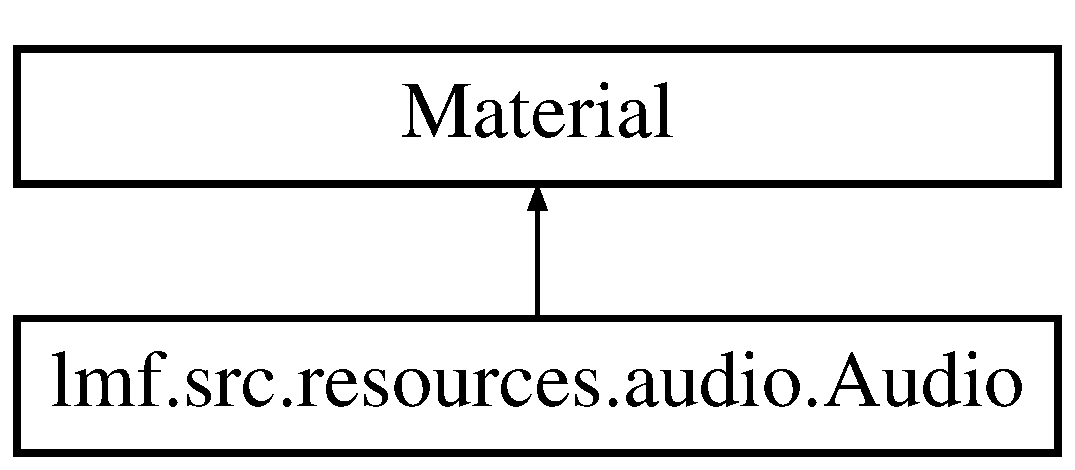
\includegraphics[height=2.000000cm]{classlmf_1_1src_1_1resources_1_1audio_1_1_audio}
\end{center}
\end{figure}
\subsection*{Public Member Functions}
\begin{DoxyCompactItemize}
\item 
def \hyperlink{classlmf_1_1src_1_1resources_1_1audio_1_1_audio_ad160d4e583ac17c4825a0432d6715685}{\+\_\+\+\_\+init\+\_\+\+\_\+}
\begin{DoxyCompactList}\small\item\em Constructor. \end{DoxyCompactList}\item 
def \hyperlink{classlmf_1_1src_1_1resources_1_1audio_1_1_audio_af6706b4ce77d04e2c5d450b83d9586ae}{\+\_\+\+\_\+del\+\_\+\+\_\+}
\begin{DoxyCompactList}\small\item\em Destructor. \end{DoxyCompactList}\end{DoxyCompactItemize}
\subsection*{Public Attributes}
\begin{DoxyCompactItemize}
\item 
\hyperlink{classlmf_1_1src_1_1resources_1_1audio_1_1_audio_a7ece3b242eefb9b0da1f5cac2a5a0859}{quality}
\item 
\hyperlink{classlmf_1_1src_1_1resources_1_1audio_1_1_audio_a18d7a7940c8b55db6dbcbe64559cf68c}{sound}
\item 
\hyperlink{classlmf_1_1src_1_1resources_1_1audio_1_1_audio_a5ff81f6d9d1f1d078a067f73594758f4}{start\+Position}
\item 
\hyperlink{classlmf_1_1src_1_1resources_1_1audio_1_1_audio_ad1640839eb1c58ca5ef9796eb7c0f559}{duration\+Of\+Effective\+Speech}
\item 
\hyperlink{classlmf_1_1src_1_1resources_1_1audio_1_1_audio_acedec7cf6764d262298924f7deb0841a}{external\+Reference}
\item 
\hyperlink{classlmf_1_1src_1_1resources_1_1audio_1_1_audio_a23a0ad9fcab348d29b306dd0c5f65736}{audio\+File\+Format}
\item 
\hyperlink{classlmf_1_1src_1_1resources_1_1audio_1_1_audio_ab8d1f2cfa0f42732f123177df3b56849}{transcription}
\end{DoxyCompactItemize}


\subsection{Detailed Description}
\hyperlink{classlmf_1_1src_1_1resources_1_1audio_1_1_audio}{Audio} is a Material subclass representing an audio recording. 

Definition at line 8 of file audio.\+py.



\subsection{Constructor \& Destructor Documentation}
\hypertarget{classlmf_1_1src_1_1resources_1_1audio_1_1_audio_ad160d4e583ac17c4825a0432d6715685}{\index{lmf\+::src\+::resources\+::audio\+::\+Audio@{lmf\+::src\+::resources\+::audio\+::\+Audio}!\+\_\+\+\_\+init\+\_\+\+\_\+@{\+\_\+\+\_\+init\+\_\+\+\_\+}}
\index{\+\_\+\+\_\+init\+\_\+\+\_\+@{\+\_\+\+\_\+init\+\_\+\+\_\+}!lmf\+::src\+::resources\+::audio\+::\+Audio@{lmf\+::src\+::resources\+::audio\+::\+Audio}}
\subsubsection[{\+\_\+\+\_\+init\+\_\+\+\_\+}]{\setlength{\rightskip}{0pt plus 5cm}def lmf.\+src.\+resources.\+audio.\+Audio.\+\_\+\+\_\+init\+\_\+\+\_\+ (
\begin{DoxyParamCaption}
\item[{}]{self}
\end{DoxyParamCaption}
)}}\label{classlmf_1_1src_1_1resources_1_1audio_1_1_audio_ad160d4e583ac17c4825a0432d6715685}


Constructor. 

\hyperlink{classlmf_1_1src_1_1resources_1_1audio_1_1_audio}{Audio} instances are owned by Form\+Representation. \begin{DoxyReturn}{Returns}
An \hyperlink{classlmf_1_1src_1_1resources_1_1audio_1_1_audio}{Audio} instance. 
\end{DoxyReturn}


Definition at line 11 of file audio.\+py.

\hypertarget{classlmf_1_1src_1_1resources_1_1audio_1_1_audio_af6706b4ce77d04e2c5d450b83d9586ae}{\index{lmf\+::src\+::resources\+::audio\+::\+Audio@{lmf\+::src\+::resources\+::audio\+::\+Audio}!\+\_\+\+\_\+del\+\_\+\+\_\+@{\+\_\+\+\_\+del\+\_\+\+\_\+}}
\index{\+\_\+\+\_\+del\+\_\+\+\_\+@{\+\_\+\+\_\+del\+\_\+\+\_\+}!lmf\+::src\+::resources\+::audio\+::\+Audio@{lmf\+::src\+::resources\+::audio\+::\+Audio}}
\subsubsection[{\+\_\+\+\_\+del\+\_\+\+\_\+}]{\setlength{\rightskip}{0pt plus 5cm}def lmf.\+src.\+resources.\+audio.\+Audio.\+\_\+\+\_\+del\+\_\+\+\_\+ (
\begin{DoxyParamCaption}
\item[{}]{self}
\end{DoxyParamCaption}
)}}\label{classlmf_1_1src_1_1resources_1_1audio_1_1_audio_af6706b4ce77d04e2c5d450b83d9586ae}


Destructor. 



Definition at line 26 of file audio.\+py.



\subsection{Member Data Documentation}
\hypertarget{classlmf_1_1src_1_1resources_1_1audio_1_1_audio_a23a0ad9fcab348d29b306dd0c5f65736}{\index{lmf\+::src\+::resources\+::audio\+::\+Audio@{lmf\+::src\+::resources\+::audio\+::\+Audio}!audio\+File\+Format@{audio\+File\+Format}}
\index{audio\+File\+Format@{audio\+File\+Format}!lmf\+::src\+::resources\+::audio\+::\+Audio@{lmf\+::src\+::resources\+::audio\+::\+Audio}}
\subsubsection[{audio\+File\+Format}]{\setlength{\rightskip}{0pt plus 5cm}lmf.\+src.\+resources.\+audio.\+Audio.\+audio\+File\+Format}}\label{classlmf_1_1src_1_1resources_1_1audio_1_1_audio_a23a0ad9fcab348d29b306dd0c5f65736}


Definition at line 23 of file audio.\+py.

\hypertarget{classlmf_1_1src_1_1resources_1_1audio_1_1_audio_ad1640839eb1c58ca5ef9796eb7c0f559}{\index{lmf\+::src\+::resources\+::audio\+::\+Audio@{lmf\+::src\+::resources\+::audio\+::\+Audio}!duration\+Of\+Effective\+Speech@{duration\+Of\+Effective\+Speech}}
\index{duration\+Of\+Effective\+Speech@{duration\+Of\+Effective\+Speech}!lmf\+::src\+::resources\+::audio\+::\+Audio@{lmf\+::src\+::resources\+::audio\+::\+Audio}}
\subsubsection[{duration\+Of\+Effective\+Speech}]{\setlength{\rightskip}{0pt plus 5cm}lmf.\+src.\+resources.\+audio.\+Audio.\+duration\+Of\+Effective\+Speech}}\label{classlmf_1_1src_1_1resources_1_1audio_1_1_audio_ad1640839eb1c58ca5ef9796eb7c0f559}


Definition at line 21 of file audio.\+py.

\hypertarget{classlmf_1_1src_1_1resources_1_1audio_1_1_audio_acedec7cf6764d262298924f7deb0841a}{\index{lmf\+::src\+::resources\+::audio\+::\+Audio@{lmf\+::src\+::resources\+::audio\+::\+Audio}!external\+Reference@{external\+Reference}}
\index{external\+Reference@{external\+Reference}!lmf\+::src\+::resources\+::audio\+::\+Audio@{lmf\+::src\+::resources\+::audio\+::\+Audio}}
\subsubsection[{external\+Reference}]{\setlength{\rightskip}{0pt plus 5cm}lmf.\+src.\+resources.\+audio.\+Audio.\+external\+Reference}}\label{classlmf_1_1src_1_1resources_1_1audio_1_1_audio_acedec7cf6764d262298924f7deb0841a}


Definition at line 22 of file audio.\+py.

\hypertarget{classlmf_1_1src_1_1resources_1_1audio_1_1_audio_a7ece3b242eefb9b0da1f5cac2a5a0859}{\index{lmf\+::src\+::resources\+::audio\+::\+Audio@{lmf\+::src\+::resources\+::audio\+::\+Audio}!quality@{quality}}
\index{quality@{quality}!lmf\+::src\+::resources\+::audio\+::\+Audio@{lmf\+::src\+::resources\+::audio\+::\+Audio}}
\subsubsection[{quality}]{\setlength{\rightskip}{0pt plus 5cm}lmf.\+src.\+resources.\+audio.\+Audio.\+quality}}\label{classlmf_1_1src_1_1resources_1_1audio_1_1_audio_a7ece3b242eefb9b0da1f5cac2a5a0859}


Definition at line 18 of file audio.\+py.

\hypertarget{classlmf_1_1src_1_1resources_1_1audio_1_1_audio_a18d7a7940c8b55db6dbcbe64559cf68c}{\index{lmf\+::src\+::resources\+::audio\+::\+Audio@{lmf\+::src\+::resources\+::audio\+::\+Audio}!sound@{sound}}
\index{sound@{sound}!lmf\+::src\+::resources\+::audio\+::\+Audio@{lmf\+::src\+::resources\+::audio\+::\+Audio}}
\subsubsection[{sound}]{\setlength{\rightskip}{0pt plus 5cm}lmf.\+src.\+resources.\+audio.\+Audio.\+sound}}\label{classlmf_1_1src_1_1resources_1_1audio_1_1_audio_a18d7a7940c8b55db6dbcbe64559cf68c}


Definition at line 19 of file audio.\+py.

\hypertarget{classlmf_1_1src_1_1resources_1_1audio_1_1_audio_a5ff81f6d9d1f1d078a067f73594758f4}{\index{lmf\+::src\+::resources\+::audio\+::\+Audio@{lmf\+::src\+::resources\+::audio\+::\+Audio}!start\+Position@{start\+Position}}
\index{start\+Position@{start\+Position}!lmf\+::src\+::resources\+::audio\+::\+Audio@{lmf\+::src\+::resources\+::audio\+::\+Audio}}
\subsubsection[{start\+Position}]{\setlength{\rightskip}{0pt plus 5cm}lmf.\+src.\+resources.\+audio.\+Audio.\+start\+Position}}\label{classlmf_1_1src_1_1resources_1_1audio_1_1_audio_a5ff81f6d9d1f1d078a067f73594758f4}


Definition at line 20 of file audio.\+py.

\hypertarget{classlmf_1_1src_1_1resources_1_1audio_1_1_audio_ab8d1f2cfa0f42732f123177df3b56849}{\index{lmf\+::src\+::resources\+::audio\+::\+Audio@{lmf\+::src\+::resources\+::audio\+::\+Audio}!transcription@{transcription}}
\index{transcription@{transcription}!lmf\+::src\+::resources\+::audio\+::\+Audio@{lmf\+::src\+::resources\+::audio\+::\+Audio}}
\subsubsection[{transcription}]{\setlength{\rightskip}{0pt plus 5cm}lmf.\+src.\+resources.\+audio.\+Audio.\+transcription}}\label{classlmf_1_1src_1_1resources_1_1audio_1_1_audio_ab8d1f2cfa0f42732f123177df3b56849}


Definition at line 24 of file audio.\+py.



The documentation for this class was generated from the following file\+:\begin{DoxyCompactItemize}
\item 
/\+Users/celine/\+Work/\+C\+N\+R\+S/workspace/\+Himal\+Co/dev/lib/lmf/src/resources/\hyperlink{audio_8py}{audio.\+py}\end{DoxyCompactItemize}

\hypertarget{classlmf_1_1src_1_1morphology_1_1component_1_1_component}{\section{lmf.\+src.\+morphology.\+component.\+Component Class Reference}
\label{classlmf_1_1src_1_1morphology_1_1component_1_1_component}\index{lmf.\+src.\+morphology.\+component.\+Component@{lmf.\+src.\+morphology.\+component.\+Component}}
}
\subsection*{Public Member Functions}
\begin{DoxyCompactItemize}
\item 
def \hyperlink{classlmf_1_1src_1_1morphology_1_1component_1_1_component_ae5d54b8fa8350b799ebbf914ef528dd7}{\+\_\+\+\_\+init\+\_\+\+\_\+}
\begin{DoxyCompactList}\small\item\em Constructor. \end{DoxyCompactList}\item 
def \hyperlink{classlmf_1_1src_1_1morphology_1_1component_1_1_component_aa9c51c8d6a9f03f3e36f8b417a8f2f1e}{\+\_\+\+\_\+del\+\_\+\+\_\+}
\begin{DoxyCompactList}\small\item\em Destructor. \end{DoxyCompactList}\item 
def \hyperlink{classlmf_1_1src_1_1morphology_1_1component_1_1_component_a4ab10116f9391089519fea00d6abdb6b}{set\+\_\+lexical\+\_\+entry}
\begin{DoxyCompactList}\small\item\em Set pointer to the component lexical entry instance. \end{DoxyCompactList}\item 
def \hyperlink{classlmf_1_1src_1_1morphology_1_1component_1_1_component_adbe6d9c8fc9cdbf9dd0a6b5c07a3afd7}{get\+\_\+lexical\+\_\+entry}
\begin{DoxyCompactList}\small\item\em Get pointed lexical entry. \end{DoxyCompactList}\item 
def \hyperlink{classlmf_1_1src_1_1morphology_1_1component_1_1_component_a78402da2b76d5031e94e90943c1cd68e}{get\+\_\+lexeme}
\begin{DoxyCompactList}\small\item\em Get component Lexical\+Entry lexeme. \end{DoxyCompactList}\end{DoxyCompactItemize}
\subsection*{Public Attributes}
\begin{DoxyCompactItemize}
\item 
\hyperlink{classlmf_1_1src_1_1morphology_1_1component_1_1_component_ad4f8453c7d8bd58fe8d364b363067b2a}{position}
\item 
\hyperlink{classlmf_1_1src_1_1morphology_1_1component_1_1_component_a90de1db1e2438bbbcd08cccbe07ad1ea}{targets}
\end{DoxyCompactItemize}


\subsection{Detailed Description}


Definition at line 6 of file component.\+py.



\subsection{Constructor \& Destructor Documentation}
\hypertarget{classlmf_1_1src_1_1morphology_1_1component_1_1_component_ae5d54b8fa8350b799ebbf914ef528dd7}{\index{lmf\+::src\+::morphology\+::component\+::\+Component@{lmf\+::src\+::morphology\+::component\+::\+Component}!\+\_\+\+\_\+init\+\_\+\+\_\+@{\+\_\+\+\_\+init\+\_\+\+\_\+}}
\index{\+\_\+\+\_\+init\+\_\+\+\_\+@{\+\_\+\+\_\+init\+\_\+\+\_\+}!lmf\+::src\+::morphology\+::component\+::\+Component@{lmf\+::src\+::morphology\+::component\+::\+Component}}
\subsubsection[{\+\_\+\+\_\+init\+\_\+\+\_\+}]{\setlength{\rightskip}{0pt plus 5cm}def lmf.\+src.\+morphology.\+component.\+Component.\+\_\+\+\_\+init\+\_\+\+\_\+ (
\begin{DoxyParamCaption}
\item[{}]{self, }
\item[{}]{position = {\ttfamily None}, }
\item[{}]{lexeme = {\ttfamily None}}
\end{DoxyParamCaption}
)}}\label{classlmf_1_1src_1_1morphology_1_1component_1_1_component_ae5d54b8fa8350b799ebbf914ef528dd7}


Constructor. 

\hyperlink{classlmf_1_1src_1_1morphology_1_1component_1_1_component}{Component} instances are owned by List\+Of\+Components. 
\begin{DoxyParams}{Parameters}
{\em position} & The position of the component in the multiword expression. \\
\hline
{\em targets} & Related lexeme. \\
\hline
\end{DoxyParams}
\begin{DoxyReturn}{Returns}
A \hyperlink{classlmf_1_1src_1_1morphology_1_1component_1_1_component}{Component} instance. 
\end{DoxyReturn}


Definition at line 7 of file component.\+py.

\hypertarget{classlmf_1_1src_1_1morphology_1_1component_1_1_component_aa9c51c8d6a9f03f3e36f8b417a8f2f1e}{\index{lmf\+::src\+::morphology\+::component\+::\+Component@{lmf\+::src\+::morphology\+::component\+::\+Component}!\+\_\+\+\_\+del\+\_\+\+\_\+@{\+\_\+\+\_\+del\+\_\+\+\_\+}}
\index{\+\_\+\+\_\+del\+\_\+\+\_\+@{\+\_\+\+\_\+del\+\_\+\+\_\+}!lmf\+::src\+::morphology\+::component\+::\+Component@{lmf\+::src\+::morphology\+::component\+::\+Component}}
\subsubsection[{\+\_\+\+\_\+del\+\_\+\+\_\+}]{\setlength{\rightskip}{0pt plus 5cm}def lmf.\+src.\+morphology.\+component.\+Component.\+\_\+\+\_\+del\+\_\+\+\_\+ (
\begin{DoxyParamCaption}
\item[{}]{self}
\end{DoxyParamCaption}
)}}\label{classlmf_1_1src_1_1morphology_1_1component_1_1_component_aa9c51c8d6a9f03f3e36f8b417a8f2f1e}


Destructor. 



Definition at line 21 of file component.\+py.



\subsection{Member Function Documentation}
\hypertarget{classlmf_1_1src_1_1morphology_1_1component_1_1_component_a78402da2b76d5031e94e90943c1cd68e}{\index{lmf\+::src\+::morphology\+::component\+::\+Component@{lmf\+::src\+::morphology\+::component\+::\+Component}!get\+\_\+lexeme@{get\+\_\+lexeme}}
\index{get\+\_\+lexeme@{get\+\_\+lexeme}!lmf\+::src\+::morphology\+::component\+::\+Component@{lmf\+::src\+::morphology\+::component\+::\+Component}}
\subsubsection[{get\+\_\+lexeme}]{\setlength{\rightskip}{0pt plus 5cm}def lmf.\+src.\+morphology.\+component.\+Component.\+get\+\_\+lexeme (
\begin{DoxyParamCaption}
\item[{}]{self}
\end{DoxyParamCaption}
)}}\label{classlmf_1_1src_1_1morphology_1_1component_1_1_component_a78402da2b76d5031e94e90943c1cd68e}


Get component Lexical\+Entry lexeme. 

\begin{DoxyReturn}{Returns}
\hyperlink{classlmf_1_1src_1_1morphology_1_1component_1_1_component}{Component} attribute 'targets'. 
\end{DoxyReturn}


Definition at line 41 of file component.\+py.

\hypertarget{classlmf_1_1src_1_1morphology_1_1component_1_1_component_adbe6d9c8fc9cdbf9dd0a6b5c07a3afd7}{\index{lmf\+::src\+::morphology\+::component\+::\+Component@{lmf\+::src\+::morphology\+::component\+::\+Component}!get\+\_\+lexical\+\_\+entry@{get\+\_\+lexical\+\_\+entry}}
\index{get\+\_\+lexical\+\_\+entry@{get\+\_\+lexical\+\_\+entry}!lmf\+::src\+::morphology\+::component\+::\+Component@{lmf\+::src\+::morphology\+::component\+::\+Component}}
\subsubsection[{get\+\_\+lexical\+\_\+entry}]{\setlength{\rightskip}{0pt plus 5cm}def lmf.\+src.\+morphology.\+component.\+Component.\+get\+\_\+lexical\+\_\+entry (
\begin{DoxyParamCaption}
\item[{}]{self}
\end{DoxyParamCaption}
)}}\label{classlmf_1_1src_1_1morphology_1_1component_1_1_component_adbe6d9c8fc9cdbf9dd0a6b5c07a3afd7}


Get pointed lexical entry. 

\begin{DoxyReturn}{Returns}
\hyperlink{classlmf_1_1src_1_1morphology_1_1component_1_1_component}{Component} private attribute '\+\_\+\+\_\+lexical\+\_\+entry'. 
\end{DoxyReturn}


Definition at line 35 of file component.\+py.

\hypertarget{classlmf_1_1src_1_1morphology_1_1component_1_1_component_a4ab10116f9391089519fea00d6abdb6b}{\index{lmf\+::src\+::morphology\+::component\+::\+Component@{lmf\+::src\+::morphology\+::component\+::\+Component}!set\+\_\+lexical\+\_\+entry@{set\+\_\+lexical\+\_\+entry}}
\index{set\+\_\+lexical\+\_\+entry@{set\+\_\+lexical\+\_\+entry}!lmf\+::src\+::morphology\+::component\+::\+Component@{lmf\+::src\+::morphology\+::component\+::\+Component}}
\subsubsection[{set\+\_\+lexical\+\_\+entry}]{\setlength{\rightskip}{0pt plus 5cm}def lmf.\+src.\+morphology.\+component.\+Component.\+set\+\_\+lexical\+\_\+entry (
\begin{DoxyParamCaption}
\item[{}]{self, }
\item[{}]{lexical\+\_\+entry}
\end{DoxyParamCaption}
)}}\label{classlmf_1_1src_1_1morphology_1_1component_1_1_component_a4ab10116f9391089519fea00d6abdb6b}


Set pointer to the component lexical entry instance. 

This function can only be called once the full dictionary has been parsed. 
\begin{DoxyParams}{Parameters}
{\em lexical\+\_\+entry} & The component Lexical\+Entry. \\
\hline
\end{DoxyParams}
\begin{DoxyReturn}{Returns}
\hyperlink{classlmf_1_1src_1_1morphology_1_1component_1_1_component}{Component} instance. 
\end{DoxyReturn}


Definition at line 27 of file component.\+py.



\subsection{Member Data Documentation}
\hypertarget{classlmf_1_1src_1_1morphology_1_1component_1_1_component_ad4f8453c7d8bd58fe8d364b363067b2a}{\index{lmf\+::src\+::morphology\+::component\+::\+Component@{lmf\+::src\+::morphology\+::component\+::\+Component}!position@{position}}
\index{position@{position}!lmf\+::src\+::morphology\+::component\+::\+Component@{lmf\+::src\+::morphology\+::component\+::\+Component}}
\subsubsection[{position}]{\setlength{\rightskip}{0pt plus 5cm}lmf.\+src.\+morphology.\+component.\+Component.\+position}}\label{classlmf_1_1src_1_1morphology_1_1component_1_1_component_ad4f8453c7d8bd58fe8d364b363067b2a}


Definition at line 14 of file component.\+py.

\hypertarget{classlmf_1_1src_1_1morphology_1_1component_1_1_component_a90de1db1e2438bbbcd08cccbe07ad1ea}{\index{lmf\+::src\+::morphology\+::component\+::\+Component@{lmf\+::src\+::morphology\+::component\+::\+Component}!targets@{targets}}
\index{targets@{targets}!lmf\+::src\+::morphology\+::component\+::\+Component@{lmf\+::src\+::morphology\+::component\+::\+Component}}
\subsubsection[{targets}]{\setlength{\rightskip}{0pt plus 5cm}lmf.\+src.\+morphology.\+component.\+Component.\+targets}}\label{classlmf_1_1src_1_1morphology_1_1component_1_1_component_a90de1db1e2438bbbcd08cccbe07ad1ea}


Definition at line 16 of file component.\+py.



The documentation for this class was generated from the following file\+:\begin{DoxyCompactItemize}
\item 
/\+Users/celine/\+Work/\+C\+N\+R\+S/workspace/\+Himal\+Co/dev/lib/lmf/src/morphology/\hyperlink{component_8py}{component.\+py}\end{DoxyCompactItemize}

\hypertarget{classlmf_1_1src_1_1mrd_1_1context_1_1_context}{\section{lmf.\+src.\+mrd.\+context.\+Context Class Reference}
\label{classlmf_1_1src_1_1mrd_1_1context_1_1_context}\index{lmf.\+src.\+mrd.\+context.\+Context@{lmf.\+src.\+mrd.\+context.\+Context}}
}


\char`\"{}\+Context is a class representing a text string that provides authentic context for the use of the word form managed by the Lemma. This class is to be distinguished from Sense Example.\char`\"{} (L\+M\+F)  


\subsection*{Public Member Functions}
\begin{DoxyCompactItemize}
\item 
def \hyperlink{classlmf_1_1src_1_1mrd_1_1context_1_1_context_acc18b0fe7b0db9c6e64e934ee67fc6a9}{\+\_\+\+\_\+init\+\_\+\+\_\+}
\begin{DoxyCompactList}\small\item\em Constructor. \end{DoxyCompactList}\item 
def \hyperlink{classlmf_1_1src_1_1mrd_1_1context_1_1_context_a490b0011c22dc5843ba7c6b176f3b72b}{\+\_\+\+\_\+del\+\_\+\+\_\+}
\begin{DoxyCompactList}\small\item\em Destructor. \end{DoxyCompactList}\item 
def \hyperlink{classlmf_1_1src_1_1mrd_1_1context_1_1_context_a4726cc609fc5d8edd15eca4f83a0712b}{set\+\_\+type}
\begin{DoxyCompactList}\small\item\em Set context type. \end{DoxyCompactList}\item 
def \hyperlink{classlmf_1_1src_1_1mrd_1_1context_1_1_context_a23bbf04da050eb93c8f0abb8a5eaf4aa}{get\+\_\+type}
\begin{DoxyCompactList}\small\item\em Get context type. \end{DoxyCompactList}\item 
def \hyperlink{classlmf_1_1src_1_1mrd_1_1context_1_1_context_ac7bd2a0ecf508291587d52cbae380e27}{create\+\_\+text\+\_\+representation}
\begin{DoxyCompactList}\small\item\em Create a text representation. \end{DoxyCompactList}\item 
def \hyperlink{classlmf_1_1src_1_1mrd_1_1context_1_1_context_a6e1527f4d3685b66da96af85a1db8d4e}{add\+\_\+text\+\_\+representation}
\begin{DoxyCompactList}\small\item\em Add a text representation to the context. \end{DoxyCompactList}\item 
def \hyperlink{classlmf_1_1src_1_1mrd_1_1context_1_1_context_a6dc9ce353b5e7e987615fec2d8a835d7}{get\+\_\+text\+\_\+representations}
\begin{DoxyCompactList}\small\item\em Get all text representations maintained by the context. \end{DoxyCompactList}\item 
def \hyperlink{classlmf_1_1src_1_1mrd_1_1context_1_1_context_a89ae6b79b719e165e5773b2035eb2ded}{get\+\_\+last\+\_\+text\+\_\+representation}
\begin{DoxyCompactList}\small\item\em Get the previously registered Text\+Representation instance. \end{DoxyCompactList}\item 
def \hyperlink{classlmf_1_1src_1_1mrd_1_1context_1_1_context_a4969405d9d78799039adce3919656fcf}{find\+\_\+written\+\_\+forms}
\begin{DoxyCompactList}\small\item\em Find written forms. \end{DoxyCompactList}\item 
def \hyperlink{classlmf_1_1src_1_1mrd_1_1context_1_1_context_a822729925a426c3ea85d6d4206c059c7}{get\+\_\+comments}
\begin{DoxyCompactList}\small\item\em Get comments. \end{DoxyCompactList}\item 
def \hyperlink{classlmf_1_1src_1_1mrd_1_1context_1_1_context_a5c25980cacb6a7268fc6144ee464ff51}{set\+\_\+written\+\_\+form}
\begin{DoxyCompactList}\small\item\em Set text representation written form, language and script. \end{DoxyCompactList}\item 
def \hyperlink{classlmf_1_1src_1_1mrd_1_1context_1_1_context_aea5b1870d2e818c89ba00055e7318395}{set\+\_\+comment}
\begin{DoxyCompactList}\small\item\em Set text representation comment. \end{DoxyCompactList}\item 
def \hyperlink{classlmf_1_1src_1_1mrd_1_1context_1_1_context_aa17fe1cc0e3bc873967f85499fed2740}{get\+\_\+speaker\+I\+D}
\begin{DoxyCompactList}\small\item\em Get related speaker identifier. \end{DoxyCompactList}\item 
def \hyperlink{classlmf_1_1src_1_1mrd_1_1context_1_1_context_a411ba47fe4581d2e3416b44fbd9ab1d9}{get\+\_\+speaker}
\begin{DoxyCompactList}\small\item\em Get speaker. \end{DoxyCompactList}\end{DoxyCompactItemize}
\subsection*{Public Attributes}
\begin{DoxyCompactItemize}
\item 
\hyperlink{classlmf_1_1src_1_1mrd_1_1context_1_1_context_a4bbfb55e0df3e37ee91abbfc59fa4111}{language}
\item 
\hyperlink{classlmf_1_1src_1_1mrd_1_1context_1_1_context_a785d657d9be0addc379745e7efa4996b}{type}
\item 
\hyperlink{classlmf_1_1src_1_1mrd_1_1context_1_1_context_a471cd19ef138a424df53621024979ba7}{text\+\_\+representation}
\begin{DoxyCompactList}\small\item\em Text\+Representation instances are owned by \hyperlink{classlmf_1_1src_1_1mrd_1_1context_1_1_context}{Context} There is zero to many Text\+Representation instances per \hyperlink{classlmf_1_1src_1_1mrd_1_1context_1_1_context}{Context}. \end{DoxyCompactList}\item 
\hyperlink{classlmf_1_1src_1_1mrd_1_1context_1_1_context_a29412f9361cee534cfa7148320e0826f}{targets}
\end{DoxyCompactItemize}


\subsection{Detailed Description}
\char`\"{}\+Context is a class representing a text string that provides authentic context for the use of the word form managed by the Lemma. This class is to be distinguished from Sense Example.\char`\"{} (L\+M\+F) 

Definition at line 10 of file context.\+py.



\subsection{Constructor \& Destructor Documentation}
\hypertarget{classlmf_1_1src_1_1mrd_1_1context_1_1_context_acc18b0fe7b0db9c6e64e934ee67fc6a9}{\index{lmf\+::src\+::mrd\+::context\+::\+Context@{lmf\+::src\+::mrd\+::context\+::\+Context}!\+\_\+\+\_\+init\+\_\+\+\_\+@{\+\_\+\+\_\+init\+\_\+\+\_\+}}
\index{\+\_\+\+\_\+init\+\_\+\+\_\+@{\+\_\+\+\_\+init\+\_\+\+\_\+}!lmf\+::src\+::mrd\+::context\+::\+Context@{lmf\+::src\+::mrd\+::context\+::\+Context}}
\subsubsection[{\+\_\+\+\_\+init\+\_\+\+\_\+}]{\setlength{\rightskip}{0pt plus 5cm}def lmf.\+src.\+mrd.\+context.\+Context.\+\_\+\+\_\+init\+\_\+\+\_\+ (
\begin{DoxyParamCaption}
\item[{}]{self, }
\item[{}]{speaker\+I\+D = {\ttfamily None}}
\end{DoxyParamCaption}
)}}\label{classlmf_1_1src_1_1mrd_1_1context_1_1_context_acc18b0fe7b0db9c6e64e934ee67fc6a9}


Constructor. 

\hyperlink{classlmf_1_1src_1_1mrd_1_1context_1_1_context}{Context} instances are owned by Sense. 
\begin{DoxyParams}{Parameters}
{\em speaker\+I\+D} & Related speaker identifier. If not provided, default value is None. \\
\hline
\end{DoxyParams}
\begin{DoxyReturn}{Returns}
A \hyperlink{classlmf_1_1src_1_1mrd_1_1context_1_1_context}{Context} instance. 
\end{DoxyReturn}


Definition at line 13 of file context.\+py.

\hypertarget{classlmf_1_1src_1_1mrd_1_1context_1_1_context_a490b0011c22dc5843ba7c6b176f3b72b}{\index{lmf\+::src\+::mrd\+::context\+::\+Context@{lmf\+::src\+::mrd\+::context\+::\+Context}!\+\_\+\+\_\+del\+\_\+\+\_\+@{\+\_\+\+\_\+del\+\_\+\+\_\+}}
\index{\+\_\+\+\_\+del\+\_\+\+\_\+@{\+\_\+\+\_\+del\+\_\+\+\_\+}!lmf\+::src\+::mrd\+::context\+::\+Context@{lmf\+::src\+::mrd\+::context\+::\+Context}}
\subsubsection[{\+\_\+\+\_\+del\+\_\+\+\_\+}]{\setlength{\rightskip}{0pt plus 5cm}def lmf.\+src.\+mrd.\+context.\+Context.\+\_\+\+\_\+del\+\_\+\+\_\+ (
\begin{DoxyParamCaption}
\item[{}]{self}
\end{DoxyParamCaption}
)}}\label{classlmf_1_1src_1_1mrd_1_1context_1_1_context_a490b0011c22dc5843ba7c6b176f3b72b}


Destructor. 

Release Text\+Representation instances. 

Definition at line 30 of file context.\+py.



\subsection{Member Function Documentation}
\hypertarget{classlmf_1_1src_1_1mrd_1_1context_1_1_context_a6e1527f4d3685b66da96af85a1db8d4e}{\index{lmf\+::src\+::mrd\+::context\+::\+Context@{lmf\+::src\+::mrd\+::context\+::\+Context}!add\+\_\+text\+\_\+representation@{add\+\_\+text\+\_\+representation}}
\index{add\+\_\+text\+\_\+representation@{add\+\_\+text\+\_\+representation}!lmf\+::src\+::mrd\+::context\+::\+Context@{lmf\+::src\+::mrd\+::context\+::\+Context}}
\subsubsection[{add\+\_\+text\+\_\+representation}]{\setlength{\rightskip}{0pt plus 5cm}def lmf.\+src.\+mrd.\+context.\+Context.\+add\+\_\+text\+\_\+representation (
\begin{DoxyParamCaption}
\item[{}]{self, }
\item[{}]{text\+\_\+representation}
\end{DoxyParamCaption}
)}}\label{classlmf_1_1src_1_1mrd_1_1context_1_1_context_a6e1527f4d3685b66da96af85a1db8d4e}


Add a text representation to the context. 


\begin{DoxyParams}{Parameters}
{\em text\+\_\+representation} & The Text\+Representation instance to add to the context. \\
\hline
\end{DoxyParams}
\begin{DoxyReturn}{Returns}
\hyperlink{classlmf_1_1src_1_1mrd_1_1context_1_1_context}{Context} instance. 
\end{DoxyReturn}


Definition at line 65 of file context.\+py.

\hypertarget{classlmf_1_1src_1_1mrd_1_1context_1_1_context_ac7bd2a0ecf508291587d52cbae380e27}{\index{lmf\+::src\+::mrd\+::context\+::\+Context@{lmf\+::src\+::mrd\+::context\+::\+Context}!create\+\_\+text\+\_\+representation@{create\+\_\+text\+\_\+representation}}
\index{create\+\_\+text\+\_\+representation@{create\+\_\+text\+\_\+representation}!lmf\+::src\+::mrd\+::context\+::\+Context@{lmf\+::src\+::mrd\+::context\+::\+Context}}
\subsubsection[{create\+\_\+text\+\_\+representation}]{\setlength{\rightskip}{0pt plus 5cm}def lmf.\+src.\+mrd.\+context.\+Context.\+create\+\_\+text\+\_\+representation (
\begin{DoxyParamCaption}
\item[{}]{self}
\end{DoxyParamCaption}
)}}\label{classlmf_1_1src_1_1mrd_1_1context_1_1_context_ac7bd2a0ecf508291587d52cbae380e27}


Create a text representation. 

\begin{DoxyReturn}{Returns}
Text\+Representation instance. 
\end{DoxyReturn}


Definition at line 59 of file context.\+py.

\hypertarget{classlmf_1_1src_1_1mrd_1_1context_1_1_context_a4969405d9d78799039adce3919656fcf}{\index{lmf\+::src\+::mrd\+::context\+::\+Context@{lmf\+::src\+::mrd\+::context\+::\+Context}!find\+\_\+written\+\_\+forms@{find\+\_\+written\+\_\+forms}}
\index{find\+\_\+written\+\_\+forms@{find\+\_\+written\+\_\+forms}!lmf\+::src\+::mrd\+::context\+::\+Context@{lmf\+::src\+::mrd\+::context\+::\+Context}}
\subsubsection[{find\+\_\+written\+\_\+forms}]{\setlength{\rightskip}{0pt plus 5cm}def lmf.\+src.\+mrd.\+context.\+Context.\+find\+\_\+written\+\_\+forms (
\begin{DoxyParamCaption}
\item[{}]{self, }
\item[{}]{language = {\ttfamily None}, }
\item[{}]{script\+\_\+name = {\ttfamily None}}
\end{DoxyParamCaption}
)}}\label{classlmf_1_1src_1_1mrd_1_1context_1_1_context_a4969405d9d78799039adce3919656fcf}


Find written forms. 

This attribute is owned by Text\+Representation. 
\begin{DoxyParams}{Parameters}
{\em language} & If given, the language to consider to retrieve the written form. \\
\hline
{\em script\+\_\+name} & If given, the script to consider to retrieve the written form. \\
\hline
\end{DoxyParams}
\begin{DoxyReturn}{Returns}
A Python list of found Text\+Representation attributes 'written\+Form'. 
\end{DoxyReturn}


Definition at line 86 of file context.\+py.

\hypertarget{classlmf_1_1src_1_1mrd_1_1context_1_1_context_a822729925a426c3ea85d6d4206c059c7}{\index{lmf\+::src\+::mrd\+::context\+::\+Context@{lmf\+::src\+::mrd\+::context\+::\+Context}!get\+\_\+comments@{get\+\_\+comments}}
\index{get\+\_\+comments@{get\+\_\+comments}!lmf\+::src\+::mrd\+::context\+::\+Context@{lmf\+::src\+::mrd\+::context\+::\+Context}}
\subsubsection[{get\+\_\+comments}]{\setlength{\rightskip}{0pt plus 5cm}def lmf.\+src.\+mrd.\+context.\+Context.\+get\+\_\+comments (
\begin{DoxyParamCaption}
\item[{}]{self}
\end{DoxyParamCaption}
)}}\label{classlmf_1_1src_1_1mrd_1_1context_1_1_context_a822729925a426c3ea85d6d4206c059c7}


Get comments. 

This attribute is owned by Text\+Representation. \begin{DoxyReturn}{Returns}
A Python list of found Text\+Representation attributes 'comment'. 
\end{DoxyReturn}


Definition at line 100 of file context.\+py.

\hypertarget{classlmf_1_1src_1_1mrd_1_1context_1_1_context_a89ae6b79b719e165e5773b2035eb2ded}{\index{lmf\+::src\+::mrd\+::context\+::\+Context@{lmf\+::src\+::mrd\+::context\+::\+Context}!get\+\_\+last\+\_\+text\+\_\+representation@{get\+\_\+last\+\_\+text\+\_\+representation}}
\index{get\+\_\+last\+\_\+text\+\_\+representation@{get\+\_\+last\+\_\+text\+\_\+representation}!lmf\+::src\+::mrd\+::context\+::\+Context@{lmf\+::src\+::mrd\+::context\+::\+Context}}
\subsubsection[{get\+\_\+last\+\_\+text\+\_\+representation}]{\setlength{\rightskip}{0pt plus 5cm}def lmf.\+src.\+mrd.\+context.\+Context.\+get\+\_\+last\+\_\+text\+\_\+representation (
\begin{DoxyParamCaption}
\item[{}]{self}
\end{DoxyParamCaption}
)}}\label{classlmf_1_1src_1_1mrd_1_1context_1_1_context_a89ae6b79b719e165e5773b2035eb2ded}


Get the previously registered Text\+Representation instance. 

\begin{DoxyReturn}{Returns}
The last element of \hyperlink{classlmf_1_1src_1_1mrd_1_1context_1_1_context}{Context} attribute 'text\+\_\+representation'. 
\end{DoxyReturn}


Definition at line 79 of file context.\+py.

\hypertarget{classlmf_1_1src_1_1mrd_1_1context_1_1_context_a411ba47fe4581d2e3416b44fbd9ab1d9}{\index{lmf\+::src\+::mrd\+::context\+::\+Context@{lmf\+::src\+::mrd\+::context\+::\+Context}!get\+\_\+speaker@{get\+\_\+speaker}}
\index{get\+\_\+speaker@{get\+\_\+speaker}!lmf\+::src\+::mrd\+::context\+::\+Context@{lmf\+::src\+::mrd\+::context\+::\+Context}}
\subsubsection[{get\+\_\+speaker}]{\setlength{\rightskip}{0pt plus 5cm}def lmf.\+src.\+mrd.\+context.\+Context.\+get\+\_\+speaker (
\begin{DoxyParamCaption}
\item[{}]{self}
\end{DoxyParamCaption}
)}}\label{classlmf_1_1src_1_1mrd_1_1context_1_1_context_a411ba47fe4581d2e3416b44fbd9ab1d9}


Get speaker. 

\begin{DoxyReturn}{Returns}
\hyperlink{classlmf_1_1src_1_1mrd_1_1context_1_1_context}{Context} private attribute '\+\_\+\+\_\+speaker'. 
\end{DoxyReturn}


Definition at line 150 of file context.\+py.

\hypertarget{classlmf_1_1src_1_1mrd_1_1context_1_1_context_aa17fe1cc0e3bc873967f85499fed2740}{\index{lmf\+::src\+::mrd\+::context\+::\+Context@{lmf\+::src\+::mrd\+::context\+::\+Context}!get\+\_\+speaker\+I\+D@{get\+\_\+speaker\+I\+D}}
\index{get\+\_\+speaker\+I\+D@{get\+\_\+speaker\+I\+D}!lmf\+::src\+::mrd\+::context\+::\+Context@{lmf\+::src\+::mrd\+::context\+::\+Context}}
\subsubsection[{get\+\_\+speaker\+I\+D}]{\setlength{\rightskip}{0pt plus 5cm}def lmf.\+src.\+mrd.\+context.\+Context.\+get\+\_\+speaker\+I\+D (
\begin{DoxyParamCaption}
\item[{}]{self}
\end{DoxyParamCaption}
)}}\label{classlmf_1_1src_1_1mrd_1_1context_1_1_context_aa17fe1cc0e3bc873967f85499fed2740}


Get related speaker identifier. 

\begin{DoxyReturn}{Returns}
\hyperlink{classlmf_1_1src_1_1mrd_1_1context_1_1_context}{Context} attribute 'targets'. 
\end{DoxyReturn}


Definition at line 144 of file context.\+py.

\hypertarget{classlmf_1_1src_1_1mrd_1_1context_1_1_context_a6dc9ce353b5e7e987615fec2d8a835d7}{\index{lmf\+::src\+::mrd\+::context\+::\+Context@{lmf\+::src\+::mrd\+::context\+::\+Context}!get\+\_\+text\+\_\+representations@{get\+\_\+text\+\_\+representations}}
\index{get\+\_\+text\+\_\+representations@{get\+\_\+text\+\_\+representations}!lmf\+::src\+::mrd\+::context\+::\+Context@{lmf\+::src\+::mrd\+::context\+::\+Context}}
\subsubsection[{get\+\_\+text\+\_\+representations}]{\setlength{\rightskip}{0pt plus 5cm}def lmf.\+src.\+mrd.\+context.\+Context.\+get\+\_\+text\+\_\+representations (
\begin{DoxyParamCaption}
\item[{}]{self}
\end{DoxyParamCaption}
)}}\label{classlmf_1_1src_1_1mrd_1_1context_1_1_context_a6dc9ce353b5e7e987615fec2d8a835d7}


Get all text representations maintained by the context. 

\begin{DoxyReturn}{Returns}
A Python list of text representations. 
\end{DoxyReturn}


Definition at line 73 of file context.\+py.

\hypertarget{classlmf_1_1src_1_1mrd_1_1context_1_1_context_a23bbf04da050eb93c8f0abb8a5eaf4aa}{\index{lmf\+::src\+::mrd\+::context\+::\+Context@{lmf\+::src\+::mrd\+::context\+::\+Context}!get\+\_\+type@{get\+\_\+type}}
\index{get\+\_\+type@{get\+\_\+type}!lmf\+::src\+::mrd\+::context\+::\+Context@{lmf\+::src\+::mrd\+::context\+::\+Context}}
\subsubsection[{get\+\_\+type}]{\setlength{\rightskip}{0pt plus 5cm}def lmf.\+src.\+mrd.\+context.\+Context.\+get\+\_\+type (
\begin{DoxyParamCaption}
\item[{}]{self}
\end{DoxyParamCaption}
)}}\label{classlmf_1_1src_1_1mrd_1_1context_1_1_context_a23bbf04da050eb93c8f0abb8a5eaf4aa}


Get context type. 

\begin{DoxyReturn}{Returns}
\hyperlink{classlmf_1_1src_1_1mrd_1_1context_1_1_context}{Context} attribute 'type'. 
\end{DoxyReturn}


Definition at line 53 of file context.\+py.

\hypertarget{classlmf_1_1src_1_1mrd_1_1context_1_1_context_aea5b1870d2e818c89ba00055e7318395}{\index{lmf\+::src\+::mrd\+::context\+::\+Context@{lmf\+::src\+::mrd\+::context\+::\+Context}!set\+\_\+comment@{set\+\_\+comment}}
\index{set\+\_\+comment@{set\+\_\+comment}!lmf\+::src\+::mrd\+::context\+::\+Context@{lmf\+::src\+::mrd\+::context\+::\+Context}}
\subsubsection[{set\+\_\+comment}]{\setlength{\rightskip}{0pt plus 5cm}def lmf.\+src.\+mrd.\+context.\+Context.\+set\+\_\+comment (
\begin{DoxyParamCaption}
\item[{}]{self, }
\item[{}]{comment}
\end{DoxyParamCaption}
)}}\label{classlmf_1_1src_1_1mrd_1_1context_1_1_context_aea5b1870d2e818c89ba00055e7318395}


Set text representation comment. 

Attribute 'comment' is owned by Text\+Representation. 
\begin{DoxyParams}{Parameters}
{\em comment} & The comment to set. \\
\hline
\end{DoxyParams}
\begin{DoxyReturn}{Returns}
\hyperlink{classlmf_1_1src_1_1mrd_1_1context_1_1_context}{Context} instance. 
\end{DoxyReturn}


Definition at line 128 of file context.\+py.

\hypertarget{classlmf_1_1src_1_1mrd_1_1context_1_1_context_a4726cc609fc5d8edd15eca4f83a0712b}{\index{lmf\+::src\+::mrd\+::context\+::\+Context@{lmf\+::src\+::mrd\+::context\+::\+Context}!set\+\_\+type@{set\+\_\+type}}
\index{set\+\_\+type@{set\+\_\+type}!lmf\+::src\+::mrd\+::context\+::\+Context@{lmf\+::src\+::mrd\+::context\+::\+Context}}
\subsubsection[{set\+\_\+type}]{\setlength{\rightskip}{0pt plus 5cm}def lmf.\+src.\+mrd.\+context.\+Context.\+set\+\_\+type (
\begin{DoxyParamCaption}
\item[{}]{self, }
\item[{}]{type}
\end{DoxyParamCaption}
)}}\label{classlmf_1_1src_1_1mrd_1_1context_1_1_context_a4726cc609fc5d8edd15eca4f83a0712b}


Set context type. 


\begin{DoxyParams}{Parameters}
{\em type} & Type of text representations, in range 'type\+\_\+example\+\_\+range' defined in '\hyperlink{range_8py}{common/range.\+py}'. \\
\hline
\end{DoxyParams}
\begin{DoxyReturn}{Returns}
\hyperlink{classlmf_1_1src_1_1mrd_1_1context_1_1_context}{Context} instance. 
\end{DoxyReturn}


Definition at line 40 of file context.\+py.

\hypertarget{classlmf_1_1src_1_1mrd_1_1context_1_1_context_a5c25980cacb6a7268fc6144ee464ff51}{\index{lmf\+::src\+::mrd\+::context\+::\+Context@{lmf\+::src\+::mrd\+::context\+::\+Context}!set\+\_\+written\+\_\+form@{set\+\_\+written\+\_\+form}}
\index{set\+\_\+written\+\_\+form@{set\+\_\+written\+\_\+form}!lmf\+::src\+::mrd\+::context\+::\+Context@{lmf\+::src\+::mrd\+::context\+::\+Context}}
\subsubsection[{set\+\_\+written\+\_\+form}]{\setlength{\rightskip}{0pt plus 5cm}def lmf.\+src.\+mrd.\+context.\+Context.\+set\+\_\+written\+\_\+form (
\begin{DoxyParamCaption}
\item[{}]{self, }
\item[{}]{written\+\_\+form, }
\item[{}]{language = {\ttfamily None}, }
\item[{}]{script\+\_\+name = {\ttfamily None}}
\end{DoxyParamCaption}
)}}\label{classlmf_1_1src_1_1mrd_1_1context_1_1_context_a5c25980cacb6a7268fc6144ee464ff51}


Set text representation written form, language and script. 

Attributes 'written\+Form', 'language' and 'script\+Name' are owned by Text\+Representation. 
\begin{DoxyParams}{Parameters}
{\em written\+\_\+form} & The written form to set. \\
\hline
{\em language} & Language of the written form. \\
\hline
{\em script\+\_\+name} & The name of the script used to write the form, e.\+g. devanagari. \\
\hline
\end{DoxyParams}
\begin{DoxyReturn}{Returns}
\hyperlink{classlmf_1_1src_1_1mrd_1_1context_1_1_context}{Context} instance. 
\end{DoxyReturn}


Definition at line 111 of file context.\+py.



\subsection{Member Data Documentation}
\hypertarget{classlmf_1_1src_1_1mrd_1_1context_1_1_context_a4bbfb55e0df3e37ee91abbfc59fa4111}{\index{lmf\+::src\+::mrd\+::context\+::\+Context@{lmf\+::src\+::mrd\+::context\+::\+Context}!language@{language}}
\index{language@{language}!lmf\+::src\+::mrd\+::context\+::\+Context@{lmf\+::src\+::mrd\+::context\+::\+Context}}
\subsubsection[{language}]{\setlength{\rightskip}{0pt plus 5cm}lmf.\+src.\+mrd.\+context.\+Context.\+language}}\label{classlmf_1_1src_1_1mrd_1_1context_1_1_context_a4bbfb55e0df3e37ee91abbfc59fa4111}


Definition at line 19 of file context.\+py.

\hypertarget{classlmf_1_1src_1_1mrd_1_1context_1_1_context_a29412f9361cee534cfa7148320e0826f}{\index{lmf\+::src\+::mrd\+::context\+::\+Context@{lmf\+::src\+::mrd\+::context\+::\+Context}!targets@{targets}}
\index{targets@{targets}!lmf\+::src\+::mrd\+::context\+::\+Context@{lmf\+::src\+::mrd\+::context\+::\+Context}}
\subsubsection[{targets}]{\setlength{\rightskip}{0pt plus 5cm}lmf.\+src.\+mrd.\+context.\+Context.\+targets}}\label{classlmf_1_1src_1_1mrd_1_1context_1_1_context_a29412f9361cee534cfa7148320e0826f}


Definition at line 25 of file context.\+py.

\hypertarget{classlmf_1_1src_1_1mrd_1_1context_1_1_context_a471cd19ef138a424df53621024979ba7}{\index{lmf\+::src\+::mrd\+::context\+::\+Context@{lmf\+::src\+::mrd\+::context\+::\+Context}!text\+\_\+representation@{text\+\_\+representation}}
\index{text\+\_\+representation@{text\+\_\+representation}!lmf\+::src\+::mrd\+::context\+::\+Context@{lmf\+::src\+::mrd\+::context\+::\+Context}}
\subsubsection[{text\+\_\+representation}]{\setlength{\rightskip}{0pt plus 5cm}lmf.\+src.\+mrd.\+context.\+Context.\+text\+\_\+representation}}\label{classlmf_1_1src_1_1mrd_1_1context_1_1_context_a471cd19ef138a424df53621024979ba7}


Text\+Representation instances are owned by \hyperlink{classlmf_1_1src_1_1mrd_1_1context_1_1_context}{Context} There is zero to many Text\+Representation instances per \hyperlink{classlmf_1_1src_1_1mrd_1_1context_1_1_context}{Context}. 



Definition at line 23 of file context.\+py.

\hypertarget{classlmf_1_1src_1_1mrd_1_1context_1_1_context_a785d657d9be0addc379745e7efa4996b}{\index{lmf\+::src\+::mrd\+::context\+::\+Context@{lmf\+::src\+::mrd\+::context\+::\+Context}!type@{type}}
\index{type@{type}!lmf\+::src\+::mrd\+::context\+::\+Context@{lmf\+::src\+::mrd\+::context\+::\+Context}}
\subsubsection[{type}]{\setlength{\rightskip}{0pt plus 5cm}lmf.\+src.\+mrd.\+context.\+Context.\+type}}\label{classlmf_1_1src_1_1mrd_1_1context_1_1_context_a785d657d9be0addc379745e7efa4996b}


Definition at line 20 of file context.\+py.



The documentation for this class was generated from the following file\+:\begin{DoxyCompactItemize}
\item 
/\+Users/celine/\+Work/\+C\+N\+R\+S/workspace/\+Himal\+Co/dev/lib/lmf/src/mrd/\hyperlink{context_8py}{context.\+py}\end{DoxyCompactItemize}

\hypertarget{classlmf_1_1src_1_1core_1_1definition_1_1_definition}{\section{lmf.\+src.\+core.\+definition.\+Definition Class Reference}
\label{classlmf_1_1src_1_1core_1_1definition_1_1_definition}\index{lmf.\+src.\+core.\+definition.\+Definition@{lmf.\+src.\+core.\+definition.\+Definition}}
}


\char`\"{}\+Definition is a class representing a narrative description of a sense. It is provided to help human users understand the meaning of a lexical entry. A Sense instance can have zero to many definitions. Each Definition instance may be associated with zero to many Text Representation instances in order to manage the text defintion in more than one language or script. In addition, the narrative description can be expressed in a different language or script than the one in the Lexical Entry instance.\char`\"{} (L\+M\+F)  


\subsection*{Public Member Functions}
\begin{DoxyCompactItemize}
\item 
def \hyperlink{classlmf_1_1src_1_1core_1_1definition_1_1_definition_a28cb2d022b2b4f699db74a6e5a904b81}{\+\_\+\+\_\+init\+\_\+\+\_\+}
\begin{DoxyCompactList}\small\item\em Constructor. \end{DoxyCompactList}\item 
def \hyperlink{classlmf_1_1src_1_1core_1_1definition_1_1_definition_a1830dd2170b25276c22d7954cd6f1b22}{\+\_\+\+\_\+del\+\_\+\+\_\+}
\begin{DoxyCompactList}\small\item\em Destructor. \end{DoxyCompactList}\item 
def \hyperlink{classlmf_1_1src_1_1core_1_1definition_1_1_definition_a40bb8bcec281527b669dce59a1f5b707}{set\+\_\+language}
\begin{DoxyCompactList}\small\item\em Set language used for definition and gloss. \end{DoxyCompactList}\item 
def \hyperlink{classlmf_1_1src_1_1core_1_1definition_1_1_definition_a8f75f0e51554d35128744fd27e7abf15}{get\+\_\+language}
\begin{DoxyCompactList}\small\item\em Get language used for definition and gloss. \end{DoxyCompactList}\item 
def \hyperlink{classlmf_1_1src_1_1core_1_1definition_1_1_definition_a959137e9ca1596287761ba0da6c35413}{set\+\_\+definition}
\begin{DoxyCompactList}\small\item\em Set definition. \end{DoxyCompactList}\item 
def \hyperlink{classlmf_1_1src_1_1core_1_1definition_1_1_definition_a68b719a7057c8b99425e7da851ec9ab8}{get\+\_\+definition}
\begin{DoxyCompactList}\small\item\em Get definition. \end{DoxyCompactList}\item 
def \hyperlink{classlmf_1_1src_1_1core_1_1definition_1_1_definition_a4242b74954f73f87b84866cbf9a17cc4}{set\+\_\+gloss}
\begin{DoxyCompactList}\small\item\em Set gloss. \end{DoxyCompactList}\item 
def \hyperlink{classlmf_1_1src_1_1core_1_1definition_1_1_definition_a95fda914d8a1946e02a53d0f4b954c6b}{get\+\_\+gloss}
\begin{DoxyCompactList}\small\item\em Get gloss. \end{DoxyCompactList}\item 
def \hyperlink{classlmf_1_1src_1_1core_1_1definition_1_1_definition_a5c0a543d23836e3ee76682135a9898c6}{create\+\_\+statement}
\begin{DoxyCompactList}\small\item\em Create a Statement instance. \end{DoxyCompactList}\item 
def \hyperlink{classlmf_1_1src_1_1core_1_1definition_1_1_definition_abda7491b111a5fd96089f9f8b2edd892}{add\+\_\+statement}
\begin{DoxyCompactList}\small\item\em Add a Statement instance to this \hyperlink{classlmf_1_1src_1_1core_1_1definition_1_1_definition}{Definition} instance. \end{DoxyCompactList}\item 
def \hyperlink{classlmf_1_1src_1_1core_1_1definition_1_1_definition_adab2b262bd4599b330b55a0afc1ea490}{get\+\_\+statements}
\begin{DoxyCompactList}\small\item\em Get all Statement instances maintained by this \hyperlink{classlmf_1_1src_1_1core_1_1definition_1_1_definition}{Definition} instance. \end{DoxyCompactList}\item 
def \hyperlink{classlmf_1_1src_1_1core_1_1definition_1_1_definition_ab82b632b8025cbfd8a773dbb5e068002}{get\+\_\+first\+\_\+statement}
\begin{DoxyCompactList}\small\item\em Get the previously registered statement. \end{DoxyCompactList}\item 
def \hyperlink{classlmf_1_1src_1_1core_1_1definition_1_1_definition_aa8733f052ebd8ee819295cd09588dbae}{set\+\_\+note}
\begin{DoxyCompactList}\small\item\em Set note, note type and language. \end{DoxyCompactList}\item 
def \hyperlink{classlmf_1_1src_1_1core_1_1definition_1_1_definition_ac69af5c460f62f3525f328f72a757f44}{find\+\_\+notes}
\begin{DoxyCompactList}\small\item\em Find notes. \end{DoxyCompactList}\item 
def \hyperlink{classlmf_1_1src_1_1core_1_1definition_1_1_definition_aa9b1e94875d795552b55ef6745dfa4aa}{set\+\_\+usage\+\_\+note}
\begin{DoxyCompactList}\small\item\em Set usage note and language. \end{DoxyCompactList}\item 
def \hyperlink{classlmf_1_1src_1_1core_1_1definition_1_1_definition_a1fb127330544e562c532ff6cc54a5153}{find\+\_\+usage\+\_\+notes}
\begin{DoxyCompactList}\small\item\em Find usage notes. \end{DoxyCompactList}\item 
def \hyperlink{classlmf_1_1src_1_1core_1_1definition_1_1_definition_ab0719eea86eb9ebe2c85b5f4d5f03317}{set\+\_\+encyclopedic\+\_\+information}
\begin{DoxyCompactList}\small\item\em Set encyclopedic information and language. \end{DoxyCompactList}\item 
def \hyperlink{classlmf_1_1src_1_1core_1_1definition_1_1_definition_a18af1b8027e329565084177a1723eec8}{find\+\_\+encyclopedic\+\_\+informations}
\begin{DoxyCompactList}\small\item\em Find encyclopedic informations. \end{DoxyCompactList}\item 
def \hyperlink{classlmf_1_1src_1_1core_1_1definition_1_1_definition_a5d622049382265fe2c289c72afeb2467}{set\+\_\+restriction}
\begin{DoxyCompactList}\small\item\em Set restriction and language. \end{DoxyCompactList}\item 
def \hyperlink{classlmf_1_1src_1_1core_1_1definition_1_1_definition_a9ae73ad0e8acd4e2712ce7c7703a9ca8}{find\+\_\+restrictions}
\begin{DoxyCompactList}\small\item\em Find restrictions. \end{DoxyCompactList}\item 
def \hyperlink{classlmf_1_1src_1_1core_1_1definition_1_1_definition_a6213c0179642486b85564672e18597d9}{set\+\_\+borrowed\+\_\+word}
\begin{DoxyCompactList}\small\item\em Set source language (in English). \end{DoxyCompactList}\item 
def \hyperlink{classlmf_1_1src_1_1core_1_1definition_1_1_definition_aa3524eaf78f9b8e4ed7b96cb946a5cf6}{get\+\_\+borrowed\+\_\+word}
\begin{DoxyCompactList}\small\item\em Get source language (in English). \end{DoxyCompactList}\item 
def \hyperlink{classlmf_1_1src_1_1core_1_1definition_1_1_definition_a3ea310dacab2046fcdbbf49e24e6d361}{set\+\_\+written\+\_\+form}
\begin{DoxyCompactList}\small\item\em Set loan word. \end{DoxyCompactList}\item 
def \hyperlink{classlmf_1_1src_1_1core_1_1definition_1_1_definition_afd3bfcee887b14bad72a5944f15fd6d3}{get\+\_\+written\+\_\+form}
\begin{DoxyCompactList}\small\item\em Get loan word. \end{DoxyCompactList}\item 
def \hyperlink{classlmf_1_1src_1_1core_1_1definition_1_1_definition_a2c6aca78fe00652774fb89c6d2653c1f}{set\+\_\+etymology}
\begin{DoxyCompactList}\small\item\em Set etymology. \end{DoxyCompactList}\item 
def \hyperlink{classlmf_1_1src_1_1core_1_1definition_1_1_definition_aa4978dd71c6d281d390e1be0a3b7fd46}{get\+\_\+etymology}
\begin{DoxyCompactList}\small\item\em Get etymology. \end{DoxyCompactList}\item 
def \hyperlink{classlmf_1_1src_1_1core_1_1definition_1_1_definition_adec12f10d1c132b1f3accb3bcace4116}{set\+\_\+etymology\+\_\+comment}
\begin{DoxyCompactList}\small\item\em Set etymology comment and language. \end{DoxyCompactList}\item 
def \hyperlink{classlmf_1_1src_1_1core_1_1definition_1_1_definition_aded2ab7ad4cf7d437a795d2d861278b4}{get\+\_\+etymology\+\_\+comment}
\begin{DoxyCompactList}\small\item\em Get etymology comment. \end{DoxyCompactList}\item 
def \hyperlink{classlmf_1_1src_1_1core_1_1definition_1_1_definition_a6e50bf6e6745b8bd9b473144f28c51b6}{get\+\_\+term\+\_\+source\+\_\+language}
\begin{DoxyCompactList}\small\item\em Get language used for the etymology comment. \end{DoxyCompactList}\item 
def \hyperlink{classlmf_1_1src_1_1core_1_1definition_1_1_definition_acc298f1512cabc232b93600e169d2f89}{set\+\_\+etymology\+\_\+gloss}
\begin{DoxyCompactList}\small\item\em Set etymology gloss. \end{DoxyCompactList}\item 
def \hyperlink{classlmf_1_1src_1_1core_1_1definition_1_1_definition_ac254957109847f1b5551ce2cc30d3998}{get\+\_\+etymology\+\_\+gloss}
\begin{DoxyCompactList}\small\item\em Get etymology gloss. \end{DoxyCompactList}\item 
def \hyperlink{classlmf_1_1src_1_1core_1_1definition_1_1_definition_a3105eceee6a4975183d655df3a731bb6}{set\+\_\+etymology\+\_\+source}
\begin{DoxyCompactList}\small\item\em Set etymology source. \end{DoxyCompactList}\item 
def \hyperlink{classlmf_1_1src_1_1core_1_1definition_1_1_definition_a112fe099d33e869c0b97de8956200d05}{get\+\_\+etymology\+\_\+source}
\begin{DoxyCompactList}\small\item\em Get etymology source. \end{DoxyCompactList}\item 
def \hyperlink{classlmf_1_1src_1_1core_1_1definition_1_1_definition_ae874984b7b123cdcedbf3cd05cbdffa9}{set\+\_\+scientific\+\_\+name}
\begin{DoxyCompactList}\small\item\em Set scientific name. \end{DoxyCompactList}\item 
def \hyperlink{classlmf_1_1src_1_1core_1_1definition_1_1_definition_a6bae0382f864136e0538bab372bbcc6d}{get\+\_\+scientific\+\_\+name}
\begin{DoxyCompactList}\small\item\em Get scientific name. \end{DoxyCompactList}\end{DoxyCompactItemize}
\subsection*{Public Attributes}
\begin{DoxyCompactItemize}
\item 
\hyperlink{classlmf_1_1src_1_1core_1_1definition_1_1_definition_aa4893a308e8f09a596edb8d7ad510a9f}{language}
\item 
\hyperlink{classlmf_1_1src_1_1core_1_1definition_1_1_definition_a11eb38a77e7ad1f45616f1bbdc1f94b2}{definition}
\item 
\hyperlink{classlmf_1_1src_1_1core_1_1definition_1_1_definition_a2ea669abd12794b2603c5cc4ea6ce45a}{gloss}
\item 
\hyperlink{classlmf_1_1src_1_1core_1_1definition_1_1_definition_a03094eec5215fece01b3412c14e357f2}{literally}
\item 
\hyperlink{classlmf_1_1src_1_1core_1_1definition_1_1_definition_abae8500dbd7200fa3d76f5599ff00d37}{text\+\_\+representation}
\begin{DoxyCompactList}\small\item\em Text\+Representation instances are owned by \hyperlink{classlmf_1_1src_1_1core_1_1definition_1_1_definition}{Definition} There is zero to many Text\+Representation instances per \hyperlink{classlmf_1_1src_1_1core_1_1definition_1_1_definition}{Definition}. \end{DoxyCompactList}\item 
\hyperlink{classlmf_1_1src_1_1core_1_1definition_1_1_definition_acc8776ce9e16149eef1968f2bb1edd79}{statement}
\begin{DoxyCompactList}\small\item\em Statement instances are owned by \hyperlink{classlmf_1_1src_1_1core_1_1definition_1_1_definition}{Definition} There is zero to many Statement instances per \hyperlink{classlmf_1_1src_1_1core_1_1definition_1_1_definition}{Definition}. \end{DoxyCompactList}\end{DoxyCompactItemize}


\subsection{Detailed Description}
\char`\"{}\+Definition is a class representing a narrative description of a sense. It is provided to help human users understand the meaning of a lexical entry. A Sense instance can have zero to many definitions. Each Definition instance may be associated with zero to many Text Representation instances in order to manage the text defintion in more than one language or script. In addition, the narrative description can be expressed in a different language or script than the one in the Lexical Entry instance.\char`\"{} (L\+M\+F) 

Definition at line 9 of file definition.\+py.



\subsection{Constructor \& Destructor Documentation}
\hypertarget{classlmf_1_1src_1_1core_1_1definition_1_1_definition_a28cb2d022b2b4f699db74a6e5a904b81}{\index{lmf\+::src\+::core\+::definition\+::\+Definition@{lmf\+::src\+::core\+::definition\+::\+Definition}!\+\_\+\+\_\+init\+\_\+\+\_\+@{\+\_\+\+\_\+init\+\_\+\+\_\+}}
\index{\+\_\+\+\_\+init\+\_\+\+\_\+@{\+\_\+\+\_\+init\+\_\+\+\_\+}!lmf\+::src\+::core\+::definition\+::\+Definition@{lmf\+::src\+::core\+::definition\+::\+Definition}}
\subsubsection[{\+\_\+\+\_\+init\+\_\+\+\_\+}]{\setlength{\rightskip}{0pt plus 5cm}def lmf.\+src.\+core.\+definition.\+Definition.\+\_\+\+\_\+init\+\_\+\+\_\+ (
\begin{DoxyParamCaption}
\item[{}]{self}
\end{DoxyParamCaption}
)}}\label{classlmf_1_1src_1_1core_1_1definition_1_1_definition_a28cb2d022b2b4f699db74a6e5a904b81}


Constructor. 

\hyperlink{classlmf_1_1src_1_1core_1_1definition_1_1_definition}{Definition} instances are owned by Sense. \begin{DoxyReturn}{Returns}
A \hyperlink{classlmf_1_1src_1_1core_1_1definition_1_1_definition}{Definition} instance. 
\end{DoxyReturn}


Definition at line 12 of file definition.\+py.

\hypertarget{classlmf_1_1src_1_1core_1_1definition_1_1_definition_a1830dd2170b25276c22d7954cd6f1b22}{\index{lmf\+::src\+::core\+::definition\+::\+Definition@{lmf\+::src\+::core\+::definition\+::\+Definition}!\+\_\+\+\_\+del\+\_\+\+\_\+@{\+\_\+\+\_\+del\+\_\+\+\_\+}}
\index{\+\_\+\+\_\+del\+\_\+\+\_\+@{\+\_\+\+\_\+del\+\_\+\+\_\+}!lmf\+::src\+::core\+::definition\+::\+Definition@{lmf\+::src\+::core\+::definition\+::\+Definition}}
\subsubsection[{\+\_\+\+\_\+del\+\_\+\+\_\+}]{\setlength{\rightskip}{0pt plus 5cm}def lmf.\+src.\+core.\+definition.\+Definition.\+\_\+\+\_\+del\+\_\+\+\_\+ (
\begin{DoxyParamCaption}
\item[{}]{self}
\end{DoxyParamCaption}
)}}\label{classlmf_1_1src_1_1core_1_1definition_1_1_definition_a1830dd2170b25276c22d7954cd6f1b22}


Destructor. 

Release Text\+Representation and Statement instances. 

Definition at line 28 of file definition.\+py.



\subsection{Member Function Documentation}
\hypertarget{classlmf_1_1src_1_1core_1_1definition_1_1_definition_abda7491b111a5fd96089f9f8b2edd892}{\index{lmf\+::src\+::core\+::definition\+::\+Definition@{lmf\+::src\+::core\+::definition\+::\+Definition}!add\+\_\+statement@{add\+\_\+statement}}
\index{add\+\_\+statement@{add\+\_\+statement}!lmf\+::src\+::core\+::definition\+::\+Definition@{lmf\+::src\+::core\+::definition\+::\+Definition}}
\subsubsection[{add\+\_\+statement}]{\setlength{\rightskip}{0pt plus 5cm}def lmf.\+src.\+core.\+definition.\+Definition.\+add\+\_\+statement (
\begin{DoxyParamCaption}
\item[{}]{self, }
\item[{}]{statement}
\end{DoxyParamCaption}
)}}\label{classlmf_1_1src_1_1core_1_1definition_1_1_definition_abda7491b111a5fd96089f9f8b2edd892}


Add a Statement instance to this \hyperlink{classlmf_1_1src_1_1core_1_1definition_1_1_definition}{Definition} instance. 


\begin{DoxyParams}{Parameters}
{\em statemement} & The Statement instance to add to the \hyperlink{classlmf_1_1src_1_1core_1_1definition_1_1_definition}{Definition} instance. \\
\hline
\end{DoxyParams}
\begin{DoxyReturn}{Returns}
\hyperlink{classlmf_1_1src_1_1core_1_1definition_1_1_definition}{Definition} instance. 
\end{DoxyReturn}


Definition at line 104 of file definition.\+py.

\hypertarget{classlmf_1_1src_1_1core_1_1definition_1_1_definition_a5c0a543d23836e3ee76682135a9898c6}{\index{lmf\+::src\+::core\+::definition\+::\+Definition@{lmf\+::src\+::core\+::definition\+::\+Definition}!create\+\_\+statement@{create\+\_\+statement}}
\index{create\+\_\+statement@{create\+\_\+statement}!lmf\+::src\+::core\+::definition\+::\+Definition@{lmf\+::src\+::core\+::definition\+::\+Definition}}
\subsubsection[{create\+\_\+statement}]{\setlength{\rightskip}{0pt plus 5cm}def lmf.\+src.\+core.\+definition.\+Definition.\+create\+\_\+statement (
\begin{DoxyParamCaption}
\item[{}]{self}
\end{DoxyParamCaption}
)}}\label{classlmf_1_1src_1_1core_1_1definition_1_1_definition_a5c0a543d23836e3ee76682135a9898c6}


Create a Statement instance. 

\begin{DoxyReturn}{Returns}
Statement instance. 
\end{DoxyReturn}


Definition at line 98 of file definition.\+py.

\hypertarget{classlmf_1_1src_1_1core_1_1definition_1_1_definition_a18af1b8027e329565084177a1723eec8}{\index{lmf\+::src\+::core\+::definition\+::\+Definition@{lmf\+::src\+::core\+::definition\+::\+Definition}!find\+\_\+encyclopedic\+\_\+informations@{find\+\_\+encyclopedic\+\_\+informations}}
\index{find\+\_\+encyclopedic\+\_\+informations@{find\+\_\+encyclopedic\+\_\+informations}!lmf\+::src\+::core\+::definition\+::\+Definition@{lmf\+::src\+::core\+::definition\+::\+Definition}}
\subsubsection[{find\+\_\+encyclopedic\+\_\+informations}]{\setlength{\rightskip}{0pt plus 5cm}def lmf.\+src.\+core.\+definition.\+Definition.\+find\+\_\+encyclopedic\+\_\+informations (
\begin{DoxyParamCaption}
\item[{}]{self, }
\item[{}]{language}
\end{DoxyParamCaption}
)}}\label{classlmf_1_1src_1_1core_1_1definition_1_1_definition_a18af1b8027e329565084177a1723eec8}


Find encyclopedic informations. 

This attribute is owned by Statement. 
\begin{DoxyParams}{Parameters}
{\em language} & The language to consider to retrieve the encyclopedic information. \\
\hline
\end{DoxyParams}
\begin{DoxyReturn}{Returns}
A Python list of found Statement attributes 'encyclopedic\+Information'. 
\end{DoxyReturn}


Definition at line 241 of file definition.\+py.

\hypertarget{classlmf_1_1src_1_1core_1_1definition_1_1_definition_ac69af5c460f62f3525f328f72a757f44}{\index{lmf\+::src\+::core\+::definition\+::\+Definition@{lmf\+::src\+::core\+::definition\+::\+Definition}!find\+\_\+notes@{find\+\_\+notes}}
\index{find\+\_\+notes@{find\+\_\+notes}!lmf\+::src\+::core\+::definition\+::\+Definition@{lmf\+::src\+::core\+::definition\+::\+Definition}}
\subsubsection[{find\+\_\+notes}]{\setlength{\rightskip}{0pt plus 5cm}def lmf.\+src.\+core.\+definition.\+Definition.\+find\+\_\+notes (
\begin{DoxyParamCaption}
\item[{}]{self, }
\item[{}]{type}
\end{DoxyParamCaption}
)}}\label{classlmf_1_1src_1_1core_1_1definition_1_1_definition_ac69af5c460f62f3525f328f72a757f44}


Find notes. 

This attribute is owned by Statement. 
\begin{DoxyParams}{Parameters}
{\em type} & The type to consider to retrieve the note. \\
\hline
\end{DoxyParams}
\begin{DoxyReturn}{Returns}
A Python list of found Statement attributes 'note'. 
\end{DoxyReturn}


Definition at line 161 of file definition.\+py.

\hypertarget{classlmf_1_1src_1_1core_1_1definition_1_1_definition_a9ae73ad0e8acd4e2712ce7c7703a9ca8}{\index{lmf\+::src\+::core\+::definition\+::\+Definition@{lmf\+::src\+::core\+::definition\+::\+Definition}!find\+\_\+restrictions@{find\+\_\+restrictions}}
\index{find\+\_\+restrictions@{find\+\_\+restrictions}!lmf\+::src\+::core\+::definition\+::\+Definition@{lmf\+::src\+::core\+::definition\+::\+Definition}}
\subsubsection[{find\+\_\+restrictions}]{\setlength{\rightskip}{0pt plus 5cm}def lmf.\+src.\+core.\+definition.\+Definition.\+find\+\_\+restrictions (
\begin{DoxyParamCaption}
\item[{}]{self, }
\item[{}]{language}
\end{DoxyParamCaption}
)}}\label{classlmf_1_1src_1_1core_1_1definition_1_1_definition_a9ae73ad0e8acd4e2712ce7c7703a9ca8}


Find restrictions. 

This attribute is owned by Statement. 
\begin{DoxyParams}{Parameters}
{\em language} & The language to consider to retrieve the restriction. \\
\hline
\end{DoxyParams}
\begin{DoxyReturn}{Returns}
A Python list of found Statement attributes 'restriction'. 
\end{DoxyReturn}


Definition at line 281 of file definition.\+py.

\hypertarget{classlmf_1_1src_1_1core_1_1definition_1_1_definition_a1fb127330544e562c532ff6cc54a5153}{\index{lmf\+::src\+::core\+::definition\+::\+Definition@{lmf\+::src\+::core\+::definition\+::\+Definition}!find\+\_\+usage\+\_\+notes@{find\+\_\+usage\+\_\+notes}}
\index{find\+\_\+usage\+\_\+notes@{find\+\_\+usage\+\_\+notes}!lmf\+::src\+::core\+::definition\+::\+Definition@{lmf\+::src\+::core\+::definition\+::\+Definition}}
\subsubsection[{find\+\_\+usage\+\_\+notes}]{\setlength{\rightskip}{0pt plus 5cm}def lmf.\+src.\+core.\+definition.\+Definition.\+find\+\_\+usage\+\_\+notes (
\begin{DoxyParamCaption}
\item[{}]{self, }
\item[{}]{language}
\end{DoxyParamCaption}
)}}\label{classlmf_1_1src_1_1core_1_1definition_1_1_definition_a1fb127330544e562c532ff6cc54a5153}


Find usage notes. 

This attribute is owned by Statement. 
\begin{DoxyParams}{Parameters}
{\em language} & The language to consider to retrieve the usage note. \\
\hline
\end{DoxyParams}
\begin{DoxyReturn}{Returns}
A Python list of found Statement attributes 'usage\+Note'. 
\end{DoxyReturn}


Definition at line 201 of file definition.\+py.

\hypertarget{classlmf_1_1src_1_1core_1_1definition_1_1_definition_aa3524eaf78f9b8e4ed7b96cb946a5cf6}{\index{lmf\+::src\+::core\+::definition\+::\+Definition@{lmf\+::src\+::core\+::definition\+::\+Definition}!get\+\_\+borrowed\+\_\+word@{get\+\_\+borrowed\+\_\+word}}
\index{get\+\_\+borrowed\+\_\+word@{get\+\_\+borrowed\+\_\+word}!lmf\+::src\+::core\+::definition\+::\+Definition@{lmf\+::src\+::core\+::definition\+::\+Definition}}
\subsubsection[{get\+\_\+borrowed\+\_\+word}]{\setlength{\rightskip}{0pt plus 5cm}def lmf.\+src.\+core.\+definition.\+Definition.\+get\+\_\+borrowed\+\_\+word (
\begin{DoxyParamCaption}
\item[{}]{self}
\end{DoxyParamCaption}
)}}\label{classlmf_1_1src_1_1core_1_1definition_1_1_definition_aa3524eaf78f9b8e4ed7b96cb946a5cf6}


Get source language (in English). 

This attribute is owned by the first Statement. \begin{DoxyReturn}{Returns}
Statement attribute 'borrowed\+Word'. 
\end{DoxyReturn}


Definition at line 308 of file definition.\+py.

\hypertarget{classlmf_1_1src_1_1core_1_1definition_1_1_definition_a68b719a7057c8b99425e7da851ec9ab8}{\index{lmf\+::src\+::core\+::definition\+::\+Definition@{lmf\+::src\+::core\+::definition\+::\+Definition}!get\+\_\+definition@{get\+\_\+definition}}
\index{get\+\_\+definition@{get\+\_\+definition}!lmf\+::src\+::core\+::definition\+::\+Definition@{lmf\+::src\+::core\+::definition\+::\+Definition}}
\subsubsection[{get\+\_\+definition}]{\setlength{\rightskip}{0pt plus 5cm}def lmf.\+src.\+core.\+definition.\+Definition.\+get\+\_\+definition (
\begin{DoxyParamCaption}
\item[{}]{self, }
\item[{}]{language = {\ttfamily None}}
\end{DoxyParamCaption}
)}}\label{classlmf_1_1src_1_1core_1_1definition_1_1_definition_a68b719a7057c8b99425e7da851ec9ab8}


Get definition. 


\begin{DoxyParams}{Parameters}
{\em language} & If this argument is given, get definition only if written in this language. \\
\hline
\end{DoxyParams}
\begin{DoxyReturn}{Returns}
The filtered \hyperlink{classlmf_1_1src_1_1core_1_1definition_1_1_definition}{Definition} attribute 'definition'. 
\end{DoxyReturn}


Definition at line 67 of file definition.\+py.

\hypertarget{classlmf_1_1src_1_1core_1_1definition_1_1_definition_aa4978dd71c6d281d390e1be0a3b7fd46}{\index{lmf\+::src\+::core\+::definition\+::\+Definition@{lmf\+::src\+::core\+::definition\+::\+Definition}!get\+\_\+etymology@{get\+\_\+etymology}}
\index{get\+\_\+etymology@{get\+\_\+etymology}!lmf\+::src\+::core\+::definition\+::\+Definition@{lmf\+::src\+::core\+::definition\+::\+Definition}}
\subsubsection[{get\+\_\+etymology}]{\setlength{\rightskip}{0pt plus 5cm}def lmf.\+src.\+core.\+definition.\+Definition.\+get\+\_\+etymology (
\begin{DoxyParamCaption}
\item[{}]{self}
\end{DoxyParamCaption}
)}}\label{classlmf_1_1src_1_1core_1_1definition_1_1_definition_aa4978dd71c6d281d390e1be0a3b7fd46}


Get etymology. 

This attribute is owned by the first Statement. \begin{DoxyReturn}{Returns}
Statement attribute 'etymology'. 
\end{DoxyReturn}


Definition at line 360 of file definition.\+py.

\hypertarget{classlmf_1_1src_1_1core_1_1definition_1_1_definition_aded2ab7ad4cf7d437a795d2d861278b4}{\index{lmf\+::src\+::core\+::definition\+::\+Definition@{lmf\+::src\+::core\+::definition\+::\+Definition}!get\+\_\+etymology\+\_\+comment@{get\+\_\+etymology\+\_\+comment}}
\index{get\+\_\+etymology\+\_\+comment@{get\+\_\+etymology\+\_\+comment}!lmf\+::src\+::core\+::definition\+::\+Definition@{lmf\+::src\+::core\+::definition\+::\+Definition}}
\subsubsection[{get\+\_\+etymology\+\_\+comment}]{\setlength{\rightskip}{0pt plus 5cm}def lmf.\+src.\+core.\+definition.\+Definition.\+get\+\_\+etymology\+\_\+comment (
\begin{DoxyParamCaption}
\item[{}]{self, }
\item[{}]{term\+\_\+source\+\_\+language = {\ttfamily None}}
\end{DoxyParamCaption}
)}}\label{classlmf_1_1src_1_1core_1_1definition_1_1_definition_aded2ab7ad4cf7d437a795d2d861278b4}


Get etymology comment. 

This attribute is owned by the first Statement. 
\begin{DoxyParams}{Parameters}
{\em term\+\_\+source\+\_\+language} & The language of the etymology comment to retrieve. \\
\hline
\end{DoxyParams}
\begin{DoxyReturn}{Returns}
Statement attribute 'etymology\+Comment'. 
\end{DoxyReturn}


Definition at line 387 of file definition.\+py.

\hypertarget{classlmf_1_1src_1_1core_1_1definition_1_1_definition_ac254957109847f1b5551ce2cc30d3998}{\index{lmf\+::src\+::core\+::definition\+::\+Definition@{lmf\+::src\+::core\+::definition\+::\+Definition}!get\+\_\+etymology\+\_\+gloss@{get\+\_\+etymology\+\_\+gloss}}
\index{get\+\_\+etymology\+\_\+gloss@{get\+\_\+etymology\+\_\+gloss}!lmf\+::src\+::core\+::definition\+::\+Definition@{lmf\+::src\+::core\+::definition\+::\+Definition}}
\subsubsection[{get\+\_\+etymology\+\_\+gloss}]{\setlength{\rightskip}{0pt plus 5cm}def lmf.\+src.\+core.\+definition.\+Definition.\+get\+\_\+etymology\+\_\+gloss (
\begin{DoxyParamCaption}
\item[{}]{self}
\end{DoxyParamCaption}
)}}\label{classlmf_1_1src_1_1core_1_1definition_1_1_definition_ac254957109847f1b5551ce2cc30d3998}


Get etymology gloss. 

This attribute is owned by the first Statement. \begin{DoxyReturn}{Returns}
Statement attribute 'etymology\+Gloss'. 
\end{DoxyReturn}


Definition at line 425 of file definition.\+py.

\hypertarget{classlmf_1_1src_1_1core_1_1definition_1_1_definition_a112fe099d33e869c0b97de8956200d05}{\index{lmf\+::src\+::core\+::definition\+::\+Definition@{lmf\+::src\+::core\+::definition\+::\+Definition}!get\+\_\+etymology\+\_\+source@{get\+\_\+etymology\+\_\+source}}
\index{get\+\_\+etymology\+\_\+source@{get\+\_\+etymology\+\_\+source}!lmf\+::src\+::core\+::definition\+::\+Definition@{lmf\+::src\+::core\+::definition\+::\+Definition}}
\subsubsection[{get\+\_\+etymology\+\_\+source}]{\setlength{\rightskip}{0pt plus 5cm}def lmf.\+src.\+core.\+definition.\+Definition.\+get\+\_\+etymology\+\_\+source (
\begin{DoxyParamCaption}
\item[{}]{self}
\end{DoxyParamCaption}
)}}\label{classlmf_1_1src_1_1core_1_1definition_1_1_definition_a112fe099d33e869c0b97de8956200d05}


Get etymology source. 

This attribute is owned by the first Statement. \begin{DoxyReturn}{Returns}
Statement attribute 'etymology\+Source'. 
\end{DoxyReturn}


Definition at line 451 of file definition.\+py.

\hypertarget{classlmf_1_1src_1_1core_1_1definition_1_1_definition_ab82b632b8025cbfd8a773dbb5e068002}{\index{lmf\+::src\+::core\+::definition\+::\+Definition@{lmf\+::src\+::core\+::definition\+::\+Definition}!get\+\_\+first\+\_\+statement@{get\+\_\+first\+\_\+statement}}
\index{get\+\_\+first\+\_\+statement@{get\+\_\+first\+\_\+statement}!lmf\+::src\+::core\+::definition\+::\+Definition@{lmf\+::src\+::core\+::definition\+::\+Definition}}
\subsubsection[{get\+\_\+first\+\_\+statement}]{\setlength{\rightskip}{0pt plus 5cm}def lmf.\+src.\+core.\+definition.\+Definition.\+get\+\_\+first\+\_\+statement (
\begin{DoxyParamCaption}
\item[{}]{self}
\end{DoxyParamCaption}
)}}\label{classlmf_1_1src_1_1core_1_1definition_1_1_definition_ab82b632b8025cbfd8a773dbb5e068002}


Get the previously registered statement. 

\begin{DoxyReturn}{Returns}
The last element of \hyperlink{classlmf_1_1src_1_1core_1_1definition_1_1_definition}{Definition} attribute 'statement'. 
\end{DoxyReturn}


Definition at line 118 of file definition.\+py.

\hypertarget{classlmf_1_1src_1_1core_1_1definition_1_1_definition_a95fda914d8a1946e02a53d0f4b954c6b}{\index{lmf\+::src\+::core\+::definition\+::\+Definition@{lmf\+::src\+::core\+::definition\+::\+Definition}!get\+\_\+gloss@{get\+\_\+gloss}}
\index{get\+\_\+gloss@{get\+\_\+gloss}!lmf\+::src\+::core\+::definition\+::\+Definition@{lmf\+::src\+::core\+::definition\+::\+Definition}}
\subsubsection[{get\+\_\+gloss}]{\setlength{\rightskip}{0pt plus 5cm}def lmf.\+src.\+core.\+definition.\+Definition.\+get\+\_\+gloss (
\begin{DoxyParamCaption}
\item[{}]{self, }
\item[{}]{language = {\ttfamily None}}
\end{DoxyParamCaption}
)}}\label{classlmf_1_1src_1_1core_1_1definition_1_1_definition_a95fda914d8a1946e02a53d0f4b954c6b}


Get gloss. 


\begin{DoxyParams}{Parameters}
{\em language} & If this argument is given, get gloss only if written in this language. \\
\hline
\end{DoxyParams}
\begin{DoxyReturn}{Returns}
The filtered \hyperlink{classlmf_1_1src_1_1core_1_1definition_1_1_definition}{Definition} attribute 'gloss'. 
\end{DoxyReturn}


Definition at line 88 of file definition.\+py.

\hypertarget{classlmf_1_1src_1_1core_1_1definition_1_1_definition_a8f75f0e51554d35128744fd27e7abf15}{\index{lmf\+::src\+::core\+::definition\+::\+Definition@{lmf\+::src\+::core\+::definition\+::\+Definition}!get\+\_\+language@{get\+\_\+language}}
\index{get\+\_\+language@{get\+\_\+language}!lmf\+::src\+::core\+::definition\+::\+Definition@{lmf\+::src\+::core\+::definition\+::\+Definition}}
\subsubsection[{get\+\_\+language}]{\setlength{\rightskip}{0pt plus 5cm}def lmf.\+src.\+core.\+definition.\+Definition.\+get\+\_\+language (
\begin{DoxyParamCaption}
\item[{}]{self}
\end{DoxyParamCaption}
)}}\label{classlmf_1_1src_1_1core_1_1definition_1_1_definition_a8f75f0e51554d35128744fd27e7abf15}


Get language used for definition and gloss. 

\begin{DoxyReturn}{Returns}
\hyperlink{classlmf_1_1src_1_1core_1_1definition_1_1_definition}{Definition} attribute 'language'. 
\end{DoxyReturn}


Definition at line 50 of file definition.\+py.

\hypertarget{classlmf_1_1src_1_1core_1_1definition_1_1_definition_a6bae0382f864136e0538bab372bbcc6d}{\index{lmf\+::src\+::core\+::definition\+::\+Definition@{lmf\+::src\+::core\+::definition\+::\+Definition}!get\+\_\+scientific\+\_\+name@{get\+\_\+scientific\+\_\+name}}
\index{get\+\_\+scientific\+\_\+name@{get\+\_\+scientific\+\_\+name}!lmf\+::src\+::core\+::definition\+::\+Definition@{lmf\+::src\+::core\+::definition\+::\+Definition}}
\subsubsection[{get\+\_\+scientific\+\_\+name}]{\setlength{\rightskip}{0pt plus 5cm}def lmf.\+src.\+core.\+definition.\+Definition.\+get\+\_\+scientific\+\_\+name (
\begin{DoxyParamCaption}
\item[{}]{self}
\end{DoxyParamCaption}
)}}\label{classlmf_1_1src_1_1core_1_1definition_1_1_definition_a6bae0382f864136e0538bab372bbcc6d}


Get scientific name. 

This attribute is owned by the first Statement. \begin{DoxyReturn}{Returns}
Statement attribute 'scientific\+Name'. 
\end{DoxyReturn}


Definition at line 477 of file definition.\+py.

\hypertarget{classlmf_1_1src_1_1core_1_1definition_1_1_definition_adab2b262bd4599b330b55a0afc1ea490}{\index{lmf\+::src\+::core\+::definition\+::\+Definition@{lmf\+::src\+::core\+::definition\+::\+Definition}!get\+\_\+statements@{get\+\_\+statements}}
\index{get\+\_\+statements@{get\+\_\+statements}!lmf\+::src\+::core\+::definition\+::\+Definition@{lmf\+::src\+::core\+::definition\+::\+Definition}}
\subsubsection[{get\+\_\+statements}]{\setlength{\rightskip}{0pt plus 5cm}def lmf.\+src.\+core.\+definition.\+Definition.\+get\+\_\+statements (
\begin{DoxyParamCaption}
\item[{}]{self}
\end{DoxyParamCaption}
)}}\label{classlmf_1_1src_1_1core_1_1definition_1_1_definition_adab2b262bd4599b330b55a0afc1ea490}


Get all Statement instances maintained by this \hyperlink{classlmf_1_1src_1_1core_1_1definition_1_1_definition}{Definition} instance. 

\begin{DoxyReturn}{Returns}
A Python list of Statement instances. 
\end{DoxyReturn}


Definition at line 112 of file definition.\+py.

\hypertarget{classlmf_1_1src_1_1core_1_1definition_1_1_definition_a6e50bf6e6745b8bd9b473144f28c51b6}{\index{lmf\+::src\+::core\+::definition\+::\+Definition@{lmf\+::src\+::core\+::definition\+::\+Definition}!get\+\_\+term\+\_\+source\+\_\+language@{get\+\_\+term\+\_\+source\+\_\+language}}
\index{get\+\_\+term\+\_\+source\+\_\+language@{get\+\_\+term\+\_\+source\+\_\+language}!lmf\+::src\+::core\+::definition\+::\+Definition@{lmf\+::src\+::core\+::definition\+::\+Definition}}
\subsubsection[{get\+\_\+term\+\_\+source\+\_\+language}]{\setlength{\rightskip}{0pt plus 5cm}def lmf.\+src.\+core.\+definition.\+Definition.\+get\+\_\+term\+\_\+source\+\_\+language (
\begin{DoxyParamCaption}
\item[{}]{self}
\end{DoxyParamCaption}
)}}\label{classlmf_1_1src_1_1core_1_1definition_1_1_definition_a6e50bf6e6745b8bd9b473144f28c51b6}


Get language used for the etymology comment. 

This attribute is owned by the first Statement. \begin{DoxyReturn}{Returns}
Statement attribute 'term\+Source\+Language'. 
\end{DoxyReturn}


Definition at line 399 of file definition.\+py.

\hypertarget{classlmf_1_1src_1_1core_1_1definition_1_1_definition_afd3bfcee887b14bad72a5944f15fd6d3}{\index{lmf\+::src\+::core\+::definition\+::\+Definition@{lmf\+::src\+::core\+::definition\+::\+Definition}!get\+\_\+written\+\_\+form@{get\+\_\+written\+\_\+form}}
\index{get\+\_\+written\+\_\+form@{get\+\_\+written\+\_\+form}!lmf\+::src\+::core\+::definition\+::\+Definition@{lmf\+::src\+::core\+::definition\+::\+Definition}}
\subsubsection[{get\+\_\+written\+\_\+form}]{\setlength{\rightskip}{0pt plus 5cm}def lmf.\+src.\+core.\+definition.\+Definition.\+get\+\_\+written\+\_\+form (
\begin{DoxyParamCaption}
\item[{}]{self}
\end{DoxyParamCaption}
)}}\label{classlmf_1_1src_1_1core_1_1definition_1_1_definition_afd3bfcee887b14bad72a5944f15fd6d3}


Get loan word. 

This attribute is owned by the first Statement. \begin{DoxyReturn}{Returns}
Statement attribute 'written\+Form'. 
\end{DoxyReturn}


Definition at line 334 of file definition.\+py.

\hypertarget{classlmf_1_1src_1_1core_1_1definition_1_1_definition_a6213c0179642486b85564672e18597d9}{\index{lmf\+::src\+::core\+::definition\+::\+Definition@{lmf\+::src\+::core\+::definition\+::\+Definition}!set\+\_\+borrowed\+\_\+word@{set\+\_\+borrowed\+\_\+word}}
\index{set\+\_\+borrowed\+\_\+word@{set\+\_\+borrowed\+\_\+word}!lmf\+::src\+::core\+::definition\+::\+Definition@{lmf\+::src\+::core\+::definition\+::\+Definition}}
\subsubsection[{set\+\_\+borrowed\+\_\+word}]{\setlength{\rightskip}{0pt plus 5cm}def lmf.\+src.\+core.\+definition.\+Definition.\+set\+\_\+borrowed\+\_\+word (
\begin{DoxyParamCaption}
\item[{}]{self, }
\item[{}]{borrowed\+\_\+word}
\end{DoxyParamCaption}
)}}\label{classlmf_1_1src_1_1core_1_1definition_1_1_definition_a6213c0179642486b85564672e18597d9}


Set source language (in English). 

Attribute 'borrowed\+Word' is owned by the first Statement. 
\begin{DoxyParams}{Parameters}
{\em borrowed\+\_\+word} & Source language. \\
\hline
\end{DoxyParams}
\begin{DoxyReturn}{Returns}
\hyperlink{classlmf_1_1src_1_1core_1_1definition_1_1_definition}{Definition} instance. 
\end{DoxyReturn}


Definition at line 293 of file definition.\+py.

\hypertarget{classlmf_1_1src_1_1core_1_1definition_1_1_definition_a959137e9ca1596287761ba0da6c35413}{\index{lmf\+::src\+::core\+::definition\+::\+Definition@{lmf\+::src\+::core\+::definition\+::\+Definition}!set\+\_\+definition@{set\+\_\+definition}}
\index{set\+\_\+definition@{set\+\_\+definition}!lmf\+::src\+::core\+::definition\+::\+Definition@{lmf\+::src\+::core\+::definition\+::\+Definition}}
\subsubsection[{set\+\_\+definition}]{\setlength{\rightskip}{0pt plus 5cm}def lmf.\+src.\+core.\+definition.\+Definition.\+set\+\_\+definition (
\begin{DoxyParamCaption}
\item[{}]{self, }
\item[{}]{definition, }
\item[{}]{language = {\ttfamily None}}
\end{DoxyParamCaption}
)}}\label{classlmf_1_1src_1_1core_1_1definition_1_1_definition_a959137e9ca1596287761ba0da6c35413}


Set definition. 


\begin{DoxyParams}{Parameters}
{\em definition} & \hyperlink{classlmf_1_1src_1_1core_1_1definition_1_1_definition}{Definition}. \\
\hline
{\em language} & Language used for the definition. \\
\hline
\end{DoxyParams}
\begin{DoxyReturn}{Returns}
\hyperlink{classlmf_1_1src_1_1core_1_1definition_1_1_definition}{Definition} instance. 
\end{DoxyReturn}


Definition at line 56 of file definition.\+py.

\hypertarget{classlmf_1_1src_1_1core_1_1definition_1_1_definition_ab0719eea86eb9ebe2c85b5f4d5f03317}{\index{lmf\+::src\+::core\+::definition\+::\+Definition@{lmf\+::src\+::core\+::definition\+::\+Definition}!set\+\_\+encyclopedic\+\_\+information@{set\+\_\+encyclopedic\+\_\+information}}
\index{set\+\_\+encyclopedic\+\_\+information@{set\+\_\+encyclopedic\+\_\+information}!lmf\+::src\+::core\+::definition\+::\+Definition@{lmf\+::src\+::core\+::definition\+::\+Definition}}
\subsubsection[{set\+\_\+encyclopedic\+\_\+information}]{\setlength{\rightskip}{0pt plus 5cm}def lmf.\+src.\+core.\+definition.\+Definition.\+set\+\_\+encyclopedic\+\_\+information (
\begin{DoxyParamCaption}
\item[{}]{self, }
\item[{}]{encyclopedic\+\_\+information, }
\item[{}]{language = {\ttfamily None}}
\end{DoxyParamCaption}
)}}\label{classlmf_1_1src_1_1core_1_1definition_1_1_definition_ab0719eea86eb9ebe2c85b5f4d5f03317}


Set encyclopedic information and language. 

These attributes are owned by Statement. 
\begin{DoxyParams}{Parameters}
{\em encyclopedic\+\_\+information} & Encyclopedic information to set. \\
\hline
{\em language} & Language used for the encyclopedic information. \\
\hline
\end{DoxyParams}
\begin{DoxyReturn}{Returns}
\hyperlink{classlmf_1_1src_1_1core_1_1definition_1_1_definition}{Definition} instance. 
\end{DoxyReturn}


Definition at line 213 of file definition.\+py.

\hypertarget{classlmf_1_1src_1_1core_1_1definition_1_1_definition_a2c6aca78fe00652774fb89c6d2653c1f}{\index{lmf\+::src\+::core\+::definition\+::\+Definition@{lmf\+::src\+::core\+::definition\+::\+Definition}!set\+\_\+etymology@{set\+\_\+etymology}}
\index{set\+\_\+etymology@{set\+\_\+etymology}!lmf\+::src\+::core\+::definition\+::\+Definition@{lmf\+::src\+::core\+::definition\+::\+Definition}}
\subsubsection[{set\+\_\+etymology}]{\setlength{\rightskip}{0pt plus 5cm}def lmf.\+src.\+core.\+definition.\+Definition.\+set\+\_\+etymology (
\begin{DoxyParamCaption}
\item[{}]{self, }
\item[{}]{etymology}
\end{DoxyParamCaption}
)}}\label{classlmf_1_1src_1_1core_1_1definition_1_1_definition_a2c6aca78fe00652774fb89c6d2653c1f}


Set etymology. 

Attribute 'etymology' is owned by the first Statement. 
\begin{DoxyParams}{Parameters}
{\em etymology} & Etymology. \\
\hline
\end{DoxyParams}
\begin{DoxyReturn}{Returns}
\hyperlink{classlmf_1_1src_1_1core_1_1definition_1_1_definition}{Definition} instance. 
\end{DoxyReturn}


Definition at line 345 of file definition.\+py.

\hypertarget{classlmf_1_1src_1_1core_1_1definition_1_1_definition_adec12f10d1c132b1f3accb3bcace4116}{\index{lmf\+::src\+::core\+::definition\+::\+Definition@{lmf\+::src\+::core\+::definition\+::\+Definition}!set\+\_\+etymology\+\_\+comment@{set\+\_\+etymology\+\_\+comment}}
\index{set\+\_\+etymology\+\_\+comment@{set\+\_\+etymology\+\_\+comment}!lmf\+::src\+::core\+::definition\+::\+Definition@{lmf\+::src\+::core\+::definition\+::\+Definition}}
\subsubsection[{set\+\_\+etymology\+\_\+comment}]{\setlength{\rightskip}{0pt plus 5cm}def lmf.\+src.\+core.\+definition.\+Definition.\+set\+\_\+etymology\+\_\+comment (
\begin{DoxyParamCaption}
\item[{}]{self, }
\item[{}]{etymology\+\_\+comment, }
\item[{}]{term\+\_\+source\+\_\+language = {\ttfamily None}}
\end{DoxyParamCaption}
)}}\label{classlmf_1_1src_1_1core_1_1definition_1_1_definition_adec12f10d1c132b1f3accb3bcace4116}


Set etymology comment and language. 

Attributes 'etymology\+Comment' and 'term\+Source\+Language' are owned by the first Statement. 
\begin{DoxyParams}{Parameters}
{\em etymology\+\_\+comment} & Etymology comment. \\
\hline
{\em term\+\_\+source\+\_\+language} & Language of the comment. \\
\hline
\end{DoxyParams}
\begin{DoxyReturn}{Returns}
\hyperlink{classlmf_1_1src_1_1core_1_1definition_1_1_definition}{Definition} instance. 
\end{DoxyReturn}


Definition at line 371 of file definition.\+py.

\hypertarget{classlmf_1_1src_1_1core_1_1definition_1_1_definition_acc298f1512cabc232b93600e169d2f89}{\index{lmf\+::src\+::core\+::definition\+::\+Definition@{lmf\+::src\+::core\+::definition\+::\+Definition}!set\+\_\+etymology\+\_\+gloss@{set\+\_\+etymology\+\_\+gloss}}
\index{set\+\_\+etymology\+\_\+gloss@{set\+\_\+etymology\+\_\+gloss}!lmf\+::src\+::core\+::definition\+::\+Definition@{lmf\+::src\+::core\+::definition\+::\+Definition}}
\subsubsection[{set\+\_\+etymology\+\_\+gloss}]{\setlength{\rightskip}{0pt plus 5cm}def lmf.\+src.\+core.\+definition.\+Definition.\+set\+\_\+etymology\+\_\+gloss (
\begin{DoxyParamCaption}
\item[{}]{self, }
\item[{}]{etymology\+\_\+gloss}
\end{DoxyParamCaption}
)}}\label{classlmf_1_1src_1_1core_1_1definition_1_1_definition_acc298f1512cabc232b93600e169d2f89}


Set etymology gloss. 

Attribute 'etymology\+Gloss' is owned by the first Statement. 
\begin{DoxyParams}{Parameters}
{\em etymology\+\_\+gloss} & Etymology gloss. \\
\hline
\end{DoxyParams}
\begin{DoxyReturn}{Returns}
\hyperlink{classlmf_1_1src_1_1core_1_1definition_1_1_definition}{Definition} instance. 
\end{DoxyReturn}


Definition at line 410 of file definition.\+py.

\hypertarget{classlmf_1_1src_1_1core_1_1definition_1_1_definition_a3105eceee6a4975183d655df3a731bb6}{\index{lmf\+::src\+::core\+::definition\+::\+Definition@{lmf\+::src\+::core\+::definition\+::\+Definition}!set\+\_\+etymology\+\_\+source@{set\+\_\+etymology\+\_\+source}}
\index{set\+\_\+etymology\+\_\+source@{set\+\_\+etymology\+\_\+source}!lmf\+::src\+::core\+::definition\+::\+Definition@{lmf\+::src\+::core\+::definition\+::\+Definition}}
\subsubsection[{set\+\_\+etymology\+\_\+source}]{\setlength{\rightskip}{0pt plus 5cm}def lmf.\+src.\+core.\+definition.\+Definition.\+set\+\_\+etymology\+\_\+source (
\begin{DoxyParamCaption}
\item[{}]{self, }
\item[{}]{etymology\+\_\+source}
\end{DoxyParamCaption}
)}}\label{classlmf_1_1src_1_1core_1_1definition_1_1_definition_a3105eceee6a4975183d655df3a731bb6}


Set etymology source. 

Attribute 'etymology\+Source' is owned by the first Statement. 
\begin{DoxyParams}{Parameters}
{\em etymology\+\_\+source} & Etymology source. \\
\hline
\end{DoxyParams}
\begin{DoxyReturn}{Returns}
\hyperlink{classlmf_1_1src_1_1core_1_1definition_1_1_definition}{Definition} instance. 
\end{DoxyReturn}


Definition at line 436 of file definition.\+py.

\hypertarget{classlmf_1_1src_1_1core_1_1definition_1_1_definition_a4242b74954f73f87b84866cbf9a17cc4}{\index{lmf\+::src\+::core\+::definition\+::\+Definition@{lmf\+::src\+::core\+::definition\+::\+Definition}!set\+\_\+gloss@{set\+\_\+gloss}}
\index{set\+\_\+gloss@{set\+\_\+gloss}!lmf\+::src\+::core\+::definition\+::\+Definition@{lmf\+::src\+::core\+::definition\+::\+Definition}}
\subsubsection[{set\+\_\+gloss}]{\setlength{\rightskip}{0pt plus 5cm}def lmf.\+src.\+core.\+definition.\+Definition.\+set\+\_\+gloss (
\begin{DoxyParamCaption}
\item[{}]{self, }
\item[{}]{gloss, }
\item[{}]{language = {\ttfamily None}}
\end{DoxyParamCaption}
)}}\label{classlmf_1_1src_1_1core_1_1definition_1_1_definition_a4242b74954f73f87b84866cbf9a17cc4}


Set gloss. 


\begin{DoxyParams}{Parameters}
{\em gloss} & Gloss. \\
\hline
{\em language} & Language used for the gloss. \\
\hline
\end{DoxyParams}
\begin{DoxyReturn}{Returns}
\hyperlink{classlmf_1_1src_1_1core_1_1definition_1_1_definition}{Definition} instance. 
\end{DoxyReturn}


Definition at line 77 of file definition.\+py.

\hypertarget{classlmf_1_1src_1_1core_1_1definition_1_1_definition_a40bb8bcec281527b669dce59a1f5b707}{\index{lmf\+::src\+::core\+::definition\+::\+Definition@{lmf\+::src\+::core\+::definition\+::\+Definition}!set\+\_\+language@{set\+\_\+language}}
\index{set\+\_\+language@{set\+\_\+language}!lmf\+::src\+::core\+::definition\+::\+Definition@{lmf\+::src\+::core\+::definition\+::\+Definition}}
\subsubsection[{set\+\_\+language}]{\setlength{\rightskip}{0pt plus 5cm}def lmf.\+src.\+core.\+definition.\+Definition.\+set\+\_\+language (
\begin{DoxyParamCaption}
\item[{}]{self, }
\item[{}]{language}
\end{DoxyParamCaption}
)}}\label{classlmf_1_1src_1_1core_1_1definition_1_1_definition_a40bb8bcec281527b669dce59a1f5b707}


Set language used for definition and gloss. 


\begin{DoxyParams}{Parameters}
{\em language} & Language used for definition and gloss. \\
\hline
\end{DoxyParams}
\begin{DoxyReturn}{Returns}
\hyperlink{classlmf_1_1src_1_1core_1_1definition_1_1_definition}{Definition} instance. 
\end{DoxyReturn}


Definition at line 39 of file definition.\+py.

\hypertarget{classlmf_1_1src_1_1core_1_1definition_1_1_definition_aa8733f052ebd8ee819295cd09588dbae}{\index{lmf\+::src\+::core\+::definition\+::\+Definition@{lmf\+::src\+::core\+::definition\+::\+Definition}!set\+\_\+note@{set\+\_\+note}}
\index{set\+\_\+note@{set\+\_\+note}!lmf\+::src\+::core\+::definition\+::\+Definition@{lmf\+::src\+::core\+::definition\+::\+Definition}}
\subsubsection[{set\+\_\+note}]{\setlength{\rightskip}{0pt plus 5cm}def lmf.\+src.\+core.\+definition.\+Definition.\+set\+\_\+note (
\begin{DoxyParamCaption}
\item[{}]{self, }
\item[{}]{note, }
\item[{}]{type = {\ttfamily None}, }
\item[{}]{language = {\ttfamily None}}
\end{DoxyParamCaption}
)}}\label{classlmf_1_1src_1_1core_1_1definition_1_1_definition_aa8733f052ebd8ee819295cd09588dbae}


Set note, note type and language. 

These attributes are owned by Statement. 
\begin{DoxyParams}{Parameters}
{\em note} & Note to set. \\
\hline
{\em type} & Type of the note. \\
\hline
{\em language} & Language used for the note. \\
\hline
\end{DoxyParams}
\begin{DoxyReturn}{Returns}
\hyperlink{classlmf_1_1src_1_1core_1_1definition_1_1_definition}{Definition} instance. 
\end{DoxyReturn}


Definition at line 125 of file definition.\+py.

\hypertarget{classlmf_1_1src_1_1core_1_1definition_1_1_definition_a5d622049382265fe2c289c72afeb2467}{\index{lmf\+::src\+::core\+::definition\+::\+Definition@{lmf\+::src\+::core\+::definition\+::\+Definition}!set\+\_\+restriction@{set\+\_\+restriction}}
\index{set\+\_\+restriction@{set\+\_\+restriction}!lmf\+::src\+::core\+::definition\+::\+Definition@{lmf\+::src\+::core\+::definition\+::\+Definition}}
\subsubsection[{set\+\_\+restriction}]{\setlength{\rightskip}{0pt plus 5cm}def lmf.\+src.\+core.\+definition.\+Definition.\+set\+\_\+restriction (
\begin{DoxyParamCaption}
\item[{}]{self, }
\item[{}]{restriction, }
\item[{}]{language = {\ttfamily None}}
\end{DoxyParamCaption}
)}}\label{classlmf_1_1src_1_1core_1_1definition_1_1_definition_a5d622049382265fe2c289c72afeb2467}


Set restriction and language. 

These attributes are owned by Statement. 
\begin{DoxyParams}{Parameters}
{\em restriction} & Restriction to set. \\
\hline
{\em language} & Language used for the restriction. \\
\hline
\end{DoxyParams}
\begin{DoxyReturn}{Returns}
\hyperlink{classlmf_1_1src_1_1core_1_1definition_1_1_definition}{Definition} instance. 
\end{DoxyReturn}


Definition at line 253 of file definition.\+py.

\hypertarget{classlmf_1_1src_1_1core_1_1definition_1_1_definition_ae874984b7b123cdcedbf3cd05cbdffa9}{\index{lmf\+::src\+::core\+::definition\+::\+Definition@{lmf\+::src\+::core\+::definition\+::\+Definition}!set\+\_\+scientific\+\_\+name@{set\+\_\+scientific\+\_\+name}}
\index{set\+\_\+scientific\+\_\+name@{set\+\_\+scientific\+\_\+name}!lmf\+::src\+::core\+::definition\+::\+Definition@{lmf\+::src\+::core\+::definition\+::\+Definition}}
\subsubsection[{set\+\_\+scientific\+\_\+name}]{\setlength{\rightskip}{0pt plus 5cm}def lmf.\+src.\+core.\+definition.\+Definition.\+set\+\_\+scientific\+\_\+name (
\begin{DoxyParamCaption}
\item[{}]{self, }
\item[{}]{scientific\+\_\+name}
\end{DoxyParamCaption}
)}}\label{classlmf_1_1src_1_1core_1_1definition_1_1_definition_ae874984b7b123cdcedbf3cd05cbdffa9}


Set scientific name. 

Attribute 'scientfic\+Name' is owned by the first Statement. 
\begin{DoxyParams}{Parameters}
{\em scientific\+\_\+name} & Scientific name. \\
\hline
\end{DoxyParams}
\begin{DoxyReturn}{Returns}
\hyperlink{classlmf_1_1src_1_1core_1_1definition_1_1_definition}{Definition} instance. 
\end{DoxyReturn}


Definition at line 462 of file definition.\+py.

\hypertarget{classlmf_1_1src_1_1core_1_1definition_1_1_definition_aa9b1e94875d795552b55ef6745dfa4aa}{\index{lmf\+::src\+::core\+::definition\+::\+Definition@{lmf\+::src\+::core\+::definition\+::\+Definition}!set\+\_\+usage\+\_\+note@{set\+\_\+usage\+\_\+note}}
\index{set\+\_\+usage\+\_\+note@{set\+\_\+usage\+\_\+note}!lmf\+::src\+::core\+::definition\+::\+Definition@{lmf\+::src\+::core\+::definition\+::\+Definition}}
\subsubsection[{set\+\_\+usage\+\_\+note}]{\setlength{\rightskip}{0pt plus 5cm}def lmf.\+src.\+core.\+definition.\+Definition.\+set\+\_\+usage\+\_\+note (
\begin{DoxyParamCaption}
\item[{}]{self, }
\item[{}]{usage\+\_\+note, }
\item[{}]{language = {\ttfamily None}}
\end{DoxyParamCaption}
)}}\label{classlmf_1_1src_1_1core_1_1definition_1_1_definition_aa9b1e94875d795552b55ef6745dfa4aa}


Set usage note and language. 

These attributes are owned by Statement. 
\begin{DoxyParams}{Parameters}
{\em usage\+\_\+note} & Usage note to set. \\
\hline
{\em language} & Language used for the usage note. \\
\hline
\end{DoxyParams}
\begin{DoxyReturn}{Returns}
\hyperlink{classlmf_1_1src_1_1core_1_1definition_1_1_definition}{Definition} instance. 
\end{DoxyReturn}


Definition at line 173 of file definition.\+py.

\hypertarget{classlmf_1_1src_1_1core_1_1definition_1_1_definition_a3ea310dacab2046fcdbbf49e24e6d361}{\index{lmf\+::src\+::core\+::definition\+::\+Definition@{lmf\+::src\+::core\+::definition\+::\+Definition}!set\+\_\+written\+\_\+form@{set\+\_\+written\+\_\+form}}
\index{set\+\_\+written\+\_\+form@{set\+\_\+written\+\_\+form}!lmf\+::src\+::core\+::definition\+::\+Definition@{lmf\+::src\+::core\+::definition\+::\+Definition}}
\subsubsection[{set\+\_\+written\+\_\+form}]{\setlength{\rightskip}{0pt plus 5cm}def lmf.\+src.\+core.\+definition.\+Definition.\+set\+\_\+written\+\_\+form (
\begin{DoxyParamCaption}
\item[{}]{self, }
\item[{}]{written\+\_\+form}
\end{DoxyParamCaption}
)}}\label{classlmf_1_1src_1_1core_1_1definition_1_1_definition_a3ea310dacab2046fcdbbf49e24e6d361}


Set loan word. 

Attribute 'written\+Form' is owned by the first Statement. 
\begin{DoxyParams}{Parameters}
{\em written\+\_\+form} & Loan word. \\
\hline
\end{DoxyParams}
\begin{DoxyReturn}{Returns}
\hyperlink{classlmf_1_1src_1_1core_1_1definition_1_1_definition}{Definition} instance. 
\end{DoxyReturn}


Definition at line 319 of file definition.\+py.



\subsection{Member Data Documentation}
\hypertarget{classlmf_1_1src_1_1core_1_1definition_1_1_definition_a11eb38a77e7ad1f45616f1bbdc1f94b2}{\index{lmf\+::src\+::core\+::definition\+::\+Definition@{lmf\+::src\+::core\+::definition\+::\+Definition}!definition@{definition}}
\index{definition@{definition}!lmf\+::src\+::core\+::definition\+::\+Definition@{lmf\+::src\+::core\+::definition\+::\+Definition}}
\subsubsection[{definition}]{\setlength{\rightskip}{0pt plus 5cm}lmf.\+src.\+core.\+definition.\+Definition.\+definition}}\label{classlmf_1_1src_1_1core_1_1definition_1_1_definition_a11eb38a77e7ad1f45616f1bbdc1f94b2}


Definition at line 18 of file definition.\+py.

\hypertarget{classlmf_1_1src_1_1core_1_1definition_1_1_definition_a2ea669abd12794b2603c5cc4ea6ce45a}{\index{lmf\+::src\+::core\+::definition\+::\+Definition@{lmf\+::src\+::core\+::definition\+::\+Definition}!gloss@{gloss}}
\index{gloss@{gloss}!lmf\+::src\+::core\+::definition\+::\+Definition@{lmf\+::src\+::core\+::definition\+::\+Definition}}
\subsubsection[{gloss}]{\setlength{\rightskip}{0pt plus 5cm}lmf.\+src.\+core.\+definition.\+Definition.\+gloss}}\label{classlmf_1_1src_1_1core_1_1definition_1_1_definition_a2ea669abd12794b2603c5cc4ea6ce45a}


Definition at line 19 of file definition.\+py.

\hypertarget{classlmf_1_1src_1_1core_1_1definition_1_1_definition_aa4893a308e8f09a596edb8d7ad510a9f}{\index{lmf\+::src\+::core\+::definition\+::\+Definition@{lmf\+::src\+::core\+::definition\+::\+Definition}!language@{language}}
\index{language@{language}!lmf\+::src\+::core\+::definition\+::\+Definition@{lmf\+::src\+::core\+::definition\+::\+Definition}}
\subsubsection[{language}]{\setlength{\rightskip}{0pt plus 5cm}lmf.\+src.\+core.\+definition.\+Definition.\+language}}\label{classlmf_1_1src_1_1core_1_1definition_1_1_definition_aa4893a308e8f09a596edb8d7ad510a9f}


Definition at line 17 of file definition.\+py.

\hypertarget{classlmf_1_1src_1_1core_1_1definition_1_1_definition_a03094eec5215fece01b3412c14e357f2}{\index{lmf\+::src\+::core\+::definition\+::\+Definition@{lmf\+::src\+::core\+::definition\+::\+Definition}!literally@{literally}}
\index{literally@{literally}!lmf\+::src\+::core\+::definition\+::\+Definition@{lmf\+::src\+::core\+::definition\+::\+Definition}}
\subsubsection[{literally}]{\setlength{\rightskip}{0pt plus 5cm}lmf.\+src.\+core.\+definition.\+Definition.\+literally}}\label{classlmf_1_1src_1_1core_1_1definition_1_1_definition_a03094eec5215fece01b3412c14e357f2}


Definition at line 20 of file definition.\+py.

\hypertarget{classlmf_1_1src_1_1core_1_1definition_1_1_definition_acc8776ce9e16149eef1968f2bb1edd79}{\index{lmf\+::src\+::core\+::definition\+::\+Definition@{lmf\+::src\+::core\+::definition\+::\+Definition}!statement@{statement}}
\index{statement@{statement}!lmf\+::src\+::core\+::definition\+::\+Definition@{lmf\+::src\+::core\+::definition\+::\+Definition}}
\subsubsection[{statement}]{\setlength{\rightskip}{0pt plus 5cm}lmf.\+src.\+core.\+definition.\+Definition.\+statement}}\label{classlmf_1_1src_1_1core_1_1definition_1_1_definition_acc8776ce9e16149eef1968f2bb1edd79}


Statement instances are owned by \hyperlink{classlmf_1_1src_1_1core_1_1definition_1_1_definition}{Definition} There is zero to many Statement instances per \hyperlink{classlmf_1_1src_1_1core_1_1definition_1_1_definition}{Definition}. 



Definition at line 26 of file definition.\+py.

\hypertarget{classlmf_1_1src_1_1core_1_1definition_1_1_definition_abae8500dbd7200fa3d76f5599ff00d37}{\index{lmf\+::src\+::core\+::definition\+::\+Definition@{lmf\+::src\+::core\+::definition\+::\+Definition}!text\+\_\+representation@{text\+\_\+representation}}
\index{text\+\_\+representation@{text\+\_\+representation}!lmf\+::src\+::core\+::definition\+::\+Definition@{lmf\+::src\+::core\+::definition\+::\+Definition}}
\subsubsection[{text\+\_\+representation}]{\setlength{\rightskip}{0pt plus 5cm}lmf.\+src.\+core.\+definition.\+Definition.\+text\+\_\+representation}}\label{classlmf_1_1src_1_1core_1_1definition_1_1_definition_abae8500dbd7200fa3d76f5599ff00d37}


Text\+Representation instances are owned by \hyperlink{classlmf_1_1src_1_1core_1_1definition_1_1_definition}{Definition} There is zero to many Text\+Representation instances per \hyperlink{classlmf_1_1src_1_1core_1_1definition_1_1_definition}{Definition}. 



Definition at line 23 of file definition.\+py.



The documentation for this class was generated from the following file\+:\begin{DoxyCompactItemize}
\item 
/\+Users/celine/\+Work/\+C\+N\+R\+S/workspace/\+Himal\+Co/dev/lib/lmf/src/core/\hyperlink{definition_8py}{definition.\+py}\end{DoxyCompactItemize}

\hypertarget{classlmf_1_1src_1_1mrd_1_1equivalent_1_1_equivalent}{\section{lmf.\+src.\+mrd.\+equivalent.\+Equivalent Class Reference}
\label{classlmf_1_1src_1_1mrd_1_1equivalent_1_1_equivalent}\index{lmf.\+src.\+mrd.\+equivalent.\+Equivalent@{lmf.\+src.\+mrd.\+equivalent.\+Equivalent}}
}


\char`\"{}\+Equivalent is a class representing the translation equivalent of the word form managed by the Lemma class.\char`\"{} (L\+M\+F)  


\subsection*{Public Member Functions}
\begin{DoxyCompactItemize}
\item 
def \hyperlink{classlmf_1_1src_1_1mrd_1_1equivalent_1_1_equivalent_a155c0d440417e4b5edccbfb761da26b8}{\+\_\+\+\_\+init\+\_\+\+\_\+}
\begin{DoxyCompactList}\small\item\em Constructor. \end{DoxyCompactList}\item 
def \hyperlink{classlmf_1_1src_1_1mrd_1_1equivalent_1_1_equivalent_ab7030713535aaa3eefe76d833add3247}{\+\_\+\+\_\+del\+\_\+\+\_\+}
\begin{DoxyCompactList}\small\item\em Destructor. \end{DoxyCompactList}\item 
def \hyperlink{classlmf_1_1src_1_1mrd_1_1equivalent_1_1_equivalent_a8355ca8b0c55bb5838c0a3638850cdc8}{set\+\_\+translation}
\begin{DoxyCompactList}\small\item\em Set translation and language. \end{DoxyCompactList}\item 
def \hyperlink{classlmf_1_1src_1_1mrd_1_1equivalent_1_1_equivalent_ade1be4a6f62723df9ef3dae07097f616}{get\+\_\+translation}
\begin{DoxyCompactList}\small\item\em Get translation. \end{DoxyCompactList}\item 
def \hyperlink{classlmf_1_1src_1_1mrd_1_1equivalent_1_1_equivalent_a702a454d6017f332b18a589f25809106}{set\+\_\+language}
\begin{DoxyCompactList}\small\item\em Set language used for translation. \end{DoxyCompactList}\item 
def \hyperlink{classlmf_1_1src_1_1mrd_1_1equivalent_1_1_equivalent_a5766b0bb65eee515a95b7eb6987cf570}{get\+\_\+language}
\begin{DoxyCompactList}\small\item\em Get language used for translation. \end{DoxyCompactList}\end{DoxyCompactItemize}
\subsection*{Public Attributes}
\begin{DoxyCompactItemize}
\item 
\hyperlink{classlmf_1_1src_1_1mrd_1_1equivalent_1_1_equivalent_a72fc245f7193aba7f5c132eee799bcde}{language}
\item 
\hyperlink{classlmf_1_1src_1_1mrd_1_1equivalent_1_1_equivalent_a77291abfc219bae6b51d8994d3c844a2}{translation}
\item 
\hyperlink{classlmf_1_1src_1_1mrd_1_1equivalent_1_1_equivalent_a6912524a8f1ac4a8203f6fa386d2f5a1}{text\+\_\+representation}
\begin{DoxyCompactList}\small\item\em Text\+Representation instances are owned by \hyperlink{classlmf_1_1src_1_1mrd_1_1equivalent_1_1_equivalent}{Equivalent} There is zero to many Text\+Representation instances per \hyperlink{classlmf_1_1src_1_1mrd_1_1equivalent_1_1_equivalent}{Equivalent}. \end{DoxyCompactList}\end{DoxyCompactItemize}


\subsection{Detailed Description}
\char`\"{}\+Equivalent is a class representing the translation equivalent of the word form managed by the Lemma class.\char`\"{} (L\+M\+F) 

Definition at line 8 of file equivalent.\+py.



\subsection{Constructor \& Destructor Documentation}
\hypertarget{classlmf_1_1src_1_1mrd_1_1equivalent_1_1_equivalent_a155c0d440417e4b5edccbfb761da26b8}{\index{lmf\+::src\+::mrd\+::equivalent\+::\+Equivalent@{lmf\+::src\+::mrd\+::equivalent\+::\+Equivalent}!\+\_\+\+\_\+init\+\_\+\+\_\+@{\+\_\+\+\_\+init\+\_\+\+\_\+}}
\index{\+\_\+\+\_\+init\+\_\+\+\_\+@{\+\_\+\+\_\+init\+\_\+\+\_\+}!lmf\+::src\+::mrd\+::equivalent\+::\+Equivalent@{lmf\+::src\+::mrd\+::equivalent\+::\+Equivalent}}
\subsubsection[{\+\_\+\+\_\+init\+\_\+\+\_\+}]{\setlength{\rightskip}{0pt plus 5cm}def lmf.\+src.\+mrd.\+equivalent.\+Equivalent.\+\_\+\+\_\+init\+\_\+\+\_\+ (
\begin{DoxyParamCaption}
\item[{}]{self}
\end{DoxyParamCaption}
)}}\label{classlmf_1_1src_1_1mrd_1_1equivalent_1_1_equivalent_a155c0d440417e4b5edccbfb761da26b8}


Constructor. 

\hyperlink{classlmf_1_1src_1_1mrd_1_1equivalent_1_1_equivalent}{Equivalent} instances are owned by Sense. \begin{DoxyReturn}{Returns}
An \hyperlink{classlmf_1_1src_1_1mrd_1_1equivalent_1_1_equivalent}{Equivalent} instance. 
\end{DoxyReturn}


Definition at line 11 of file equivalent.\+py.

\hypertarget{classlmf_1_1src_1_1mrd_1_1equivalent_1_1_equivalent_ab7030713535aaa3eefe76d833add3247}{\index{lmf\+::src\+::mrd\+::equivalent\+::\+Equivalent@{lmf\+::src\+::mrd\+::equivalent\+::\+Equivalent}!\+\_\+\+\_\+del\+\_\+\+\_\+@{\+\_\+\+\_\+del\+\_\+\+\_\+}}
\index{\+\_\+\+\_\+del\+\_\+\+\_\+@{\+\_\+\+\_\+del\+\_\+\+\_\+}!lmf\+::src\+::mrd\+::equivalent\+::\+Equivalent@{lmf\+::src\+::mrd\+::equivalent\+::\+Equivalent}}
\subsubsection[{\+\_\+\+\_\+del\+\_\+\+\_\+}]{\setlength{\rightskip}{0pt plus 5cm}def lmf.\+src.\+mrd.\+equivalent.\+Equivalent.\+\_\+\+\_\+del\+\_\+\+\_\+ (
\begin{DoxyParamCaption}
\item[{}]{self}
\end{DoxyParamCaption}
)}}\label{classlmf_1_1src_1_1mrd_1_1equivalent_1_1_equivalent_ab7030713535aaa3eefe76d833add3247}


Destructor. 

Release Text\+Representation instances. 

Definition at line 22 of file equivalent.\+py.



\subsection{Member Function Documentation}
\hypertarget{classlmf_1_1src_1_1mrd_1_1equivalent_1_1_equivalent_a5766b0bb65eee515a95b7eb6987cf570}{\index{lmf\+::src\+::mrd\+::equivalent\+::\+Equivalent@{lmf\+::src\+::mrd\+::equivalent\+::\+Equivalent}!get\+\_\+language@{get\+\_\+language}}
\index{get\+\_\+language@{get\+\_\+language}!lmf\+::src\+::mrd\+::equivalent\+::\+Equivalent@{lmf\+::src\+::mrd\+::equivalent\+::\+Equivalent}}
\subsubsection[{get\+\_\+language}]{\setlength{\rightskip}{0pt plus 5cm}def lmf.\+src.\+mrd.\+equivalent.\+Equivalent.\+get\+\_\+language (
\begin{DoxyParamCaption}
\item[{}]{self}
\end{DoxyParamCaption}
)}}\label{classlmf_1_1src_1_1mrd_1_1equivalent_1_1_equivalent_a5766b0bb65eee515a95b7eb6987cf570}


Get language used for translation. 

\begin{DoxyReturn}{Returns}
\hyperlink{classlmf_1_1src_1_1mrd_1_1equivalent_1_1_equivalent}{Equivalent} attribute 'language'. 
\end{DoxyReturn}


Definition at line 61 of file equivalent.\+py.

\hypertarget{classlmf_1_1src_1_1mrd_1_1equivalent_1_1_equivalent_ade1be4a6f62723df9ef3dae07097f616}{\index{lmf\+::src\+::mrd\+::equivalent\+::\+Equivalent@{lmf\+::src\+::mrd\+::equivalent\+::\+Equivalent}!get\+\_\+translation@{get\+\_\+translation}}
\index{get\+\_\+translation@{get\+\_\+translation}!lmf\+::src\+::mrd\+::equivalent\+::\+Equivalent@{lmf\+::src\+::mrd\+::equivalent\+::\+Equivalent}}
\subsubsection[{get\+\_\+translation}]{\setlength{\rightskip}{0pt plus 5cm}def lmf.\+src.\+mrd.\+equivalent.\+Equivalent.\+get\+\_\+translation (
\begin{DoxyParamCaption}
\item[{}]{self, }
\item[{}]{language = {\ttfamily None}}
\end{DoxyParamCaption}
)}}\label{classlmf_1_1src_1_1mrd_1_1equivalent_1_1_equivalent_ade1be4a6f62723df9ef3dae07097f616}


Get translation. 


\begin{DoxyParams}{Parameters}
{\em language} & If this argument is given, get translation only if written in this language. \\
\hline
\end{DoxyParams}
\begin{DoxyReturn}{Returns}
The filtered \hyperlink{classlmf_1_1src_1_1mrd_1_1equivalent_1_1_equivalent}{Equivalent} attribute 'translation'. 
\end{DoxyReturn}


Definition at line 43 of file equivalent.\+py.

\hypertarget{classlmf_1_1src_1_1mrd_1_1equivalent_1_1_equivalent_a702a454d6017f332b18a589f25809106}{\index{lmf\+::src\+::mrd\+::equivalent\+::\+Equivalent@{lmf\+::src\+::mrd\+::equivalent\+::\+Equivalent}!set\+\_\+language@{set\+\_\+language}}
\index{set\+\_\+language@{set\+\_\+language}!lmf\+::src\+::mrd\+::equivalent\+::\+Equivalent@{lmf\+::src\+::mrd\+::equivalent\+::\+Equivalent}}
\subsubsection[{set\+\_\+language}]{\setlength{\rightskip}{0pt plus 5cm}def lmf.\+src.\+mrd.\+equivalent.\+Equivalent.\+set\+\_\+language (
\begin{DoxyParamCaption}
\item[{}]{self, }
\item[{}]{language}
\end{DoxyParamCaption}
)}}\label{classlmf_1_1src_1_1mrd_1_1equivalent_1_1_equivalent_a702a454d6017f332b18a589f25809106}


Set language used for translation. 


\begin{DoxyParams}{Parameters}
{\em language} & Language used for the translation. \\
\hline
\end{DoxyParams}
\begin{DoxyReturn}{Returns}
\hyperlink{classlmf_1_1src_1_1mrd_1_1equivalent_1_1_equivalent}{Equivalent} instance. 
\end{DoxyReturn}


Definition at line 51 of file equivalent.\+py.

\hypertarget{classlmf_1_1src_1_1mrd_1_1equivalent_1_1_equivalent_a8355ca8b0c55bb5838c0a3638850cdc8}{\index{lmf\+::src\+::mrd\+::equivalent\+::\+Equivalent@{lmf\+::src\+::mrd\+::equivalent\+::\+Equivalent}!set\+\_\+translation@{set\+\_\+translation}}
\index{set\+\_\+translation@{set\+\_\+translation}!lmf\+::src\+::mrd\+::equivalent\+::\+Equivalent@{lmf\+::src\+::mrd\+::equivalent\+::\+Equivalent}}
\subsubsection[{set\+\_\+translation}]{\setlength{\rightskip}{0pt plus 5cm}def lmf.\+src.\+mrd.\+equivalent.\+Equivalent.\+set\+\_\+translation (
\begin{DoxyParamCaption}
\item[{}]{self, }
\item[{}]{translation, }
\item[{}]{language = {\ttfamily None}}
\end{DoxyParamCaption}
)}}\label{classlmf_1_1src_1_1mrd_1_1equivalent_1_1_equivalent_a8355ca8b0c55bb5838c0a3638850cdc8}


Set translation and language. 


\begin{DoxyParams}{Parameters}
{\em translation} & The translation to set. \\
\hline
{\em language} & Language used for the translation. \\
\hline
\end{DoxyParams}
\begin{DoxyReturn}{Returns}
\hyperlink{classlmf_1_1src_1_1mrd_1_1equivalent_1_1_equivalent}{Equivalent} instance. 
\end{DoxyReturn}


Definition at line 30 of file equivalent.\+py.



\subsection{Member Data Documentation}
\hypertarget{classlmf_1_1src_1_1mrd_1_1equivalent_1_1_equivalent_a72fc245f7193aba7f5c132eee799bcde}{\index{lmf\+::src\+::mrd\+::equivalent\+::\+Equivalent@{lmf\+::src\+::mrd\+::equivalent\+::\+Equivalent}!language@{language}}
\index{language@{language}!lmf\+::src\+::mrd\+::equivalent\+::\+Equivalent@{lmf\+::src\+::mrd\+::equivalent\+::\+Equivalent}}
\subsubsection[{language}]{\setlength{\rightskip}{0pt plus 5cm}lmf.\+src.\+mrd.\+equivalent.\+Equivalent.\+language}}\label{classlmf_1_1src_1_1mrd_1_1equivalent_1_1_equivalent_a72fc245f7193aba7f5c132eee799bcde}


Definition at line 16 of file equivalent.\+py.

\hypertarget{classlmf_1_1src_1_1mrd_1_1equivalent_1_1_equivalent_a6912524a8f1ac4a8203f6fa386d2f5a1}{\index{lmf\+::src\+::mrd\+::equivalent\+::\+Equivalent@{lmf\+::src\+::mrd\+::equivalent\+::\+Equivalent}!text\+\_\+representation@{text\+\_\+representation}}
\index{text\+\_\+representation@{text\+\_\+representation}!lmf\+::src\+::mrd\+::equivalent\+::\+Equivalent@{lmf\+::src\+::mrd\+::equivalent\+::\+Equivalent}}
\subsubsection[{text\+\_\+representation}]{\setlength{\rightskip}{0pt plus 5cm}lmf.\+src.\+mrd.\+equivalent.\+Equivalent.\+text\+\_\+representation}}\label{classlmf_1_1src_1_1mrd_1_1equivalent_1_1_equivalent_a6912524a8f1ac4a8203f6fa386d2f5a1}


Text\+Representation instances are owned by \hyperlink{classlmf_1_1src_1_1mrd_1_1equivalent_1_1_equivalent}{Equivalent} There is zero to many Text\+Representation instances per \hyperlink{classlmf_1_1src_1_1mrd_1_1equivalent_1_1_equivalent}{Equivalent}. 



Definition at line 20 of file equivalent.\+py.

\hypertarget{classlmf_1_1src_1_1mrd_1_1equivalent_1_1_equivalent_a77291abfc219bae6b51d8994d3c844a2}{\index{lmf\+::src\+::mrd\+::equivalent\+::\+Equivalent@{lmf\+::src\+::mrd\+::equivalent\+::\+Equivalent}!translation@{translation}}
\index{translation@{translation}!lmf\+::src\+::mrd\+::equivalent\+::\+Equivalent@{lmf\+::src\+::mrd\+::equivalent\+::\+Equivalent}}
\subsubsection[{translation}]{\setlength{\rightskip}{0pt plus 5cm}lmf.\+src.\+mrd.\+equivalent.\+Equivalent.\+translation}}\label{classlmf_1_1src_1_1mrd_1_1equivalent_1_1_equivalent_a77291abfc219bae6b51d8994d3c844a2}


Definition at line 17 of file equivalent.\+py.



The documentation for this class was generated from the following file\+:\begin{DoxyCompactItemize}
\item 
/\+Users/celine/\+Work/\+C\+N\+R\+S/workspace/\+Himal\+Co/dev/lib/lmf/src/mrd/\hyperlink{equivalent_8py}{equivalent.\+py}\end{DoxyCompactItemize}

\hypertarget{classlmf_1_1src_1_1utils_1_1error__handling_1_1_error}{\section{lmf.\+src.\+utils.\+error\+\_\+handling.\+Error Class Reference}
\label{classlmf_1_1src_1_1utils_1_1error__handling_1_1_error}\index{lmf.\+src.\+utils.\+error\+\_\+handling.\+Error@{lmf.\+src.\+utils.\+error\+\_\+handling.\+Error}}
}


Base class for exceptions in this library.  


Inheritance diagram for lmf.\+src.\+utils.\+error\+\_\+handling.\+Error\+:\begin{figure}[H]
\begin{center}
\leavevmode
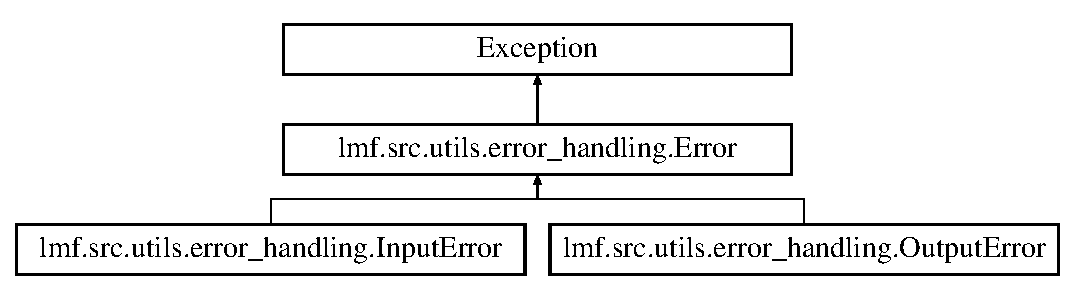
\includegraphics[height=3.000000cm]{classlmf_1_1src_1_1utils_1_1error__handling_1_1_error}
\end{center}
\end{figure}
\subsection*{Public Member Functions}
\begin{DoxyCompactItemize}
\item 
def \hyperlink{classlmf_1_1src_1_1utils_1_1error__handling_1_1_error_a7ef901bcd33f6064d695302b1167d811}{\+\_\+\+\_\+init\+\_\+\+\_\+}
\begin{DoxyCompactList}\small\item\em Constructor. \end{DoxyCompactList}\item 
def \hyperlink{classlmf_1_1src_1_1utils_1_1error__handling_1_1_error_a1904e4b7091d08a68e43a0e13b5d10e6}{\+\_\+\+\_\+str\+\_\+\+\_\+}
\begin{DoxyCompactList}\small\item\em Build the string to be displayed. \end{DoxyCompactList}\item 
def \hyperlink{classlmf_1_1src_1_1utils_1_1error__handling_1_1_error_af74fa5546dd2777e4d4b23b84b98cf9d}{handle}
\begin{DoxyCompactList}\small\item\em Define behavior to follow in case this error is caught\+: diplay error and exit program. \end{DoxyCompactList}\end{DoxyCompactItemize}
\subsection*{Public Attributes}
\begin{DoxyCompactItemize}
\item 
\hyperlink{classlmf_1_1src_1_1utils_1_1error__handling_1_1_error_ad949ea867656445f2db40f53c3369209}{msg}
\item 
\hyperlink{classlmf_1_1src_1_1utils_1_1error__handling_1_1_error_ab3bb063176871fe118580d16667ee5b2}{excp}
\item 
\hyperlink{classlmf_1_1src_1_1utils_1_1error__handling_1_1_error_a6a83c5628792d5ae735d52a9af4709d4}{frame\+\_\+info}
\end{DoxyCompactItemize}


\subsection{Detailed Description}
Base class for exceptions in this library. 

Definition at line 3 of file error\+\_\+handling.\+py.



\subsection{Constructor \& Destructor Documentation}
\hypertarget{classlmf_1_1src_1_1utils_1_1error__handling_1_1_error_a7ef901bcd33f6064d695302b1167d811}{\index{lmf\+::src\+::utils\+::error\+\_\+handling\+::\+Error@{lmf\+::src\+::utils\+::error\+\_\+handling\+::\+Error}!\+\_\+\+\_\+init\+\_\+\+\_\+@{\+\_\+\+\_\+init\+\_\+\+\_\+}}
\index{\+\_\+\+\_\+init\+\_\+\+\_\+@{\+\_\+\+\_\+init\+\_\+\+\_\+}!lmf\+::src\+::utils\+::error\+\_\+handling\+::\+Error@{lmf\+::src\+::utils\+::error\+\_\+handling\+::\+Error}}
\subsubsection[{\+\_\+\+\_\+init\+\_\+\+\_\+}]{\setlength{\rightskip}{0pt plus 5cm}def lmf.\+src.\+utils.\+error\+\_\+handling.\+Error.\+\_\+\+\_\+init\+\_\+\+\_\+ (
\begin{DoxyParamCaption}
\item[{}]{self, }
\item[{}]{msg, }
\item[{}]{excp = {\ttfamily None}}
\end{DoxyParamCaption}
)}}\label{classlmf_1_1src_1_1utils_1_1error__handling_1_1_error_a7ef901bcd33f6064d695302b1167d811}


Constructor. 


\begin{DoxyParams}{Parameters}
{\em msg} & String to be reported to user. \\
\hline
{\em excp} & Raised system exception if any\+: I\+O\+Error, Keyboard\+Interrupt, System\+Exit, Index\+Error, Key\+Error, Attribute\+Error, Type\+Error, Name\+Error, Unbound\+Local\+Error, Value\+Error. \\
\hline
\end{DoxyParams}
\begin{DoxyReturn}{Returns}
An \hyperlink{classlmf_1_1src_1_1utils_1_1error__handling_1_1_error}{Error} instance. 
\end{DoxyReturn}


Definition at line 6 of file error\+\_\+handling.\+py.



\subsection{Member Function Documentation}
\hypertarget{classlmf_1_1src_1_1utils_1_1error__handling_1_1_error_a1904e4b7091d08a68e43a0e13b5d10e6}{\index{lmf\+::src\+::utils\+::error\+\_\+handling\+::\+Error@{lmf\+::src\+::utils\+::error\+\_\+handling\+::\+Error}!\+\_\+\+\_\+str\+\_\+\+\_\+@{\+\_\+\+\_\+str\+\_\+\+\_\+}}
\index{\+\_\+\+\_\+str\+\_\+\+\_\+@{\+\_\+\+\_\+str\+\_\+\+\_\+}!lmf\+::src\+::utils\+::error\+\_\+handling\+::\+Error@{lmf\+::src\+::utils\+::error\+\_\+handling\+::\+Error}}
\subsubsection[{\+\_\+\+\_\+str\+\_\+\+\_\+}]{\setlength{\rightskip}{0pt plus 5cm}def lmf.\+src.\+utils.\+error\+\_\+handling.\+Error.\+\_\+\+\_\+str\+\_\+\+\_\+ (
\begin{DoxyParamCaption}
\item[{}]{self}
\end{DoxyParamCaption}
)}}\label{classlmf_1_1src_1_1utils_1_1error__handling_1_1_error_a1904e4b7091d08a68e43a0e13b5d10e6}


Build the string to be displayed. 

\begin{DoxyReturn}{Returns}
A Python string. 
\end{DoxyReturn}


Definition at line 18 of file error\+\_\+handling.\+py.

\hypertarget{classlmf_1_1src_1_1utils_1_1error__handling_1_1_error_af74fa5546dd2777e4d4b23b84b98cf9d}{\index{lmf\+::src\+::utils\+::error\+\_\+handling\+::\+Error@{lmf\+::src\+::utils\+::error\+\_\+handling\+::\+Error}!handle@{handle}}
\index{handle@{handle}!lmf\+::src\+::utils\+::error\+\_\+handling\+::\+Error@{lmf\+::src\+::utils\+::error\+\_\+handling\+::\+Error}}
\subsubsection[{handle}]{\setlength{\rightskip}{0pt plus 5cm}def lmf.\+src.\+utils.\+error\+\_\+handling.\+Error.\+handle (
\begin{DoxyParamCaption}
\item[{}]{self}
\end{DoxyParamCaption}
)}}\label{classlmf_1_1src_1_1utils_1_1error__handling_1_1_error_af74fa5546dd2777e4d4b23b84b98cf9d}


Define behavior to follow in case this error is caught\+: diplay error and exit program. 



Definition at line 30 of file error\+\_\+handling.\+py.



\subsection{Member Data Documentation}
\hypertarget{classlmf_1_1src_1_1utils_1_1error__handling_1_1_error_ab3bb063176871fe118580d16667ee5b2}{\index{lmf\+::src\+::utils\+::error\+\_\+handling\+::\+Error@{lmf\+::src\+::utils\+::error\+\_\+handling\+::\+Error}!excp@{excp}}
\index{excp@{excp}!lmf\+::src\+::utils\+::error\+\_\+handling\+::\+Error@{lmf\+::src\+::utils\+::error\+\_\+handling\+::\+Error}}
\subsubsection[{excp}]{\setlength{\rightskip}{0pt plus 5cm}lmf.\+src.\+utils.\+error\+\_\+handling.\+Error.\+excp}}\label{classlmf_1_1src_1_1utils_1_1error__handling_1_1_error_ab3bb063176871fe118580d16667ee5b2}


Definition at line 13 of file error\+\_\+handling.\+py.

\hypertarget{classlmf_1_1src_1_1utils_1_1error__handling_1_1_error_a6a83c5628792d5ae735d52a9af4709d4}{\index{lmf\+::src\+::utils\+::error\+\_\+handling\+::\+Error@{lmf\+::src\+::utils\+::error\+\_\+handling\+::\+Error}!frame\+\_\+info@{frame\+\_\+info}}
\index{frame\+\_\+info@{frame\+\_\+info}!lmf\+::src\+::utils\+::error\+\_\+handling\+::\+Error@{lmf\+::src\+::utils\+::error\+\_\+handling\+::\+Error}}
\subsubsection[{frame\+\_\+info}]{\setlength{\rightskip}{0pt plus 5cm}lmf.\+src.\+utils.\+error\+\_\+handling.\+Error.\+frame\+\_\+info}}\label{classlmf_1_1src_1_1utils_1_1error__handling_1_1_error_a6a83c5628792d5ae735d52a9af4709d4}


Definition at line 16 of file error\+\_\+handling.\+py.

\hypertarget{classlmf_1_1src_1_1utils_1_1error__handling_1_1_error_ad949ea867656445f2db40f53c3369209}{\index{lmf\+::src\+::utils\+::error\+\_\+handling\+::\+Error@{lmf\+::src\+::utils\+::error\+\_\+handling\+::\+Error}!msg@{msg}}
\index{msg@{msg}!lmf\+::src\+::utils\+::error\+\_\+handling\+::\+Error@{lmf\+::src\+::utils\+::error\+\_\+handling\+::\+Error}}
\subsubsection[{msg}]{\setlength{\rightskip}{0pt plus 5cm}lmf.\+src.\+utils.\+error\+\_\+handling.\+Error.\+msg}}\label{classlmf_1_1src_1_1utils_1_1error__handling_1_1_error_ad949ea867656445f2db40f53c3369209}


Definition at line 12 of file error\+\_\+handling.\+py.



The documentation for this class was generated from the following file\+:\begin{DoxyCompactItemize}
\item 
/\+Users/celine/\+Work/\+C\+N\+R\+S/workspace/\+Himal\+Co/dev/lib/lmf/src/utils/\hyperlink{error__handling_8py}{error\+\_\+handling.\+py}\end{DoxyCompactItemize}

\hypertarget{classlmf_1_1src_1_1core_1_1form_1_1_form}{\section{lmf.\+src.\+core.\+form.\+Form Class Reference}
\label{classlmf_1_1src_1_1core_1_1form_1_1_form}\index{lmf.\+src.\+core.\+form.\+Form@{lmf.\+src.\+core.\+form.\+Form}}
}


\char`\"{}\+Form is an abstract class representing a lexeme, a morphological variant of a lexeme or a morph. The Form class allows subclasses.\char`\"{} (L\+M\+F)  


\subsection*{Public Member Functions}
\begin{DoxyCompactItemize}
\item 
def \hyperlink{classlmf_1_1src_1_1core_1_1form_1_1_form_a5d8193e2ae85d0844470137d14504ae1}{\+\_\+\+\_\+init\+\_\+\+\_\+}
\begin{DoxyCompactList}\small\item\em As \hyperlink{classlmf_1_1src_1_1core_1_1form_1_1_form}{Form} is an abstract class, constructor raises an error. \end{DoxyCompactList}\item 
def \hyperlink{classlmf_1_1src_1_1core_1_1form_1_1_form_a4efc5b5afe396103742f2be36f3ada35}{\+\_\+\+\_\+del\+\_\+\+\_\+}
\begin{DoxyCompactList}\small\item\em As \hyperlink{classlmf_1_1src_1_1core_1_1form_1_1_form}{Form} is an abstract class, desctructor raises an error. \end{DoxyCompactList}\item 
def \hyperlink{classlmf_1_1src_1_1core_1_1form_1_1_form_a6b5179aebc5f1a51875d3cc5301c6f84}{\+\_\+\+\_\+new\+\_\+\+\_\+}
\begin{DoxyCompactList}\small\item\em Private initialization called from \hyperlink{classlmf_1_1src_1_1core_1_1form_1_1_form}{Form} subclasses. \end{DoxyCompactList}\end{DoxyCompactItemize}
\subsection*{Public Attributes}
\begin{DoxyCompactItemize}
\item 
\hyperlink{classlmf_1_1src_1_1core_1_1form_1_1_form_a81a147d40e70054d06b4ad90fd523a8f}{form\+\_\+representation}
\begin{DoxyCompactList}\small\item\em Form\+Representation instances are owned by \hyperlink{classlmf_1_1src_1_1core_1_1form_1_1_form}{Form} subclasses There is zero to many Form\+Representation instances per \hyperlink{classlmf_1_1src_1_1core_1_1form_1_1_form}{Form} subclass. \end{DoxyCompactList}\end{DoxyCompactItemize}


\subsection{Detailed Description}
\char`\"{}\+Form is an abstract class representing a lexeme, a morphological variant of a lexeme or a morph. The Form class allows subclasses.\char`\"{} (L\+M\+F) 

Definition at line 6 of file form.\+py.



\subsection{Constructor \& Destructor Documentation}
\hypertarget{classlmf_1_1src_1_1core_1_1form_1_1_form_a5d8193e2ae85d0844470137d14504ae1}{\index{lmf\+::src\+::core\+::form\+::\+Form@{lmf\+::src\+::core\+::form\+::\+Form}!\+\_\+\+\_\+init\+\_\+\+\_\+@{\+\_\+\+\_\+init\+\_\+\+\_\+}}
\index{\+\_\+\+\_\+init\+\_\+\+\_\+@{\+\_\+\+\_\+init\+\_\+\+\_\+}!lmf\+::src\+::core\+::form\+::\+Form@{lmf\+::src\+::core\+::form\+::\+Form}}
\subsubsection[{\+\_\+\+\_\+init\+\_\+\+\_\+}]{\setlength{\rightskip}{0pt plus 5cm}def lmf.\+src.\+core.\+form.\+Form.\+\_\+\+\_\+init\+\_\+\+\_\+ (
\begin{DoxyParamCaption}
\item[{}]{self}
\end{DoxyParamCaption}
)}}\label{classlmf_1_1src_1_1core_1_1form_1_1_form_a5d8193e2ae85d0844470137d14504ae1}


As \hyperlink{classlmf_1_1src_1_1core_1_1form_1_1_form}{Form} is an abstract class, constructor raises an error. 



Definition at line 9 of file form.\+py.

\hypertarget{classlmf_1_1src_1_1core_1_1form_1_1_form_a4efc5b5afe396103742f2be36f3ada35}{\index{lmf\+::src\+::core\+::form\+::\+Form@{lmf\+::src\+::core\+::form\+::\+Form}!\+\_\+\+\_\+del\+\_\+\+\_\+@{\+\_\+\+\_\+del\+\_\+\+\_\+}}
\index{\+\_\+\+\_\+del\+\_\+\+\_\+@{\+\_\+\+\_\+del\+\_\+\+\_\+}!lmf\+::src\+::core\+::form\+::\+Form@{lmf\+::src\+::core\+::form\+::\+Form}}
\subsubsection[{\+\_\+\+\_\+del\+\_\+\+\_\+}]{\setlength{\rightskip}{0pt plus 5cm}def lmf.\+src.\+core.\+form.\+Form.\+\_\+\+\_\+del\+\_\+\+\_\+ (
\begin{DoxyParamCaption}
\item[{}]{self}
\end{DoxyParamCaption}
)}}\label{classlmf_1_1src_1_1core_1_1form_1_1_form_a4efc5b5afe396103742f2be36f3ada35}


As \hyperlink{classlmf_1_1src_1_1core_1_1form_1_1_form}{Form} is an abstract class, desctructor raises an error. 



Definition at line 14 of file form.\+py.



\subsection{Member Function Documentation}
\hypertarget{classlmf_1_1src_1_1core_1_1form_1_1_form_a6b5179aebc5f1a51875d3cc5301c6f84}{\index{lmf\+::src\+::core\+::form\+::\+Form@{lmf\+::src\+::core\+::form\+::\+Form}!\+\_\+\+\_\+new\+\_\+\+\_\+@{\+\_\+\+\_\+new\+\_\+\+\_\+}}
\index{\+\_\+\+\_\+new\+\_\+\+\_\+@{\+\_\+\+\_\+new\+\_\+\+\_\+}!lmf\+::src\+::core\+::form\+::\+Form@{lmf\+::src\+::core\+::form\+::\+Form}}
\subsubsection[{\+\_\+\+\_\+new\+\_\+\+\_\+}]{\setlength{\rightskip}{0pt plus 5cm}def lmf.\+src.\+core.\+form.\+Form.\+\_\+\+\_\+new\+\_\+\+\_\+ (
\begin{DoxyParamCaption}
\item[{}]{self}
\end{DoxyParamCaption}
)}}\label{classlmf_1_1src_1_1core_1_1form_1_1_form_a6b5179aebc5f1a51875d3cc5301c6f84}


Private initialization called from \hyperlink{classlmf_1_1src_1_1core_1_1form_1_1_form}{Form} subclasses. 

\hyperlink{classlmf_1_1src_1_1core_1_1form_1_1_form}{Form} subinstances are owned by Lexical\+Entry. 

Definition at line 19 of file form.\+py.



\subsection{Member Data Documentation}
\hypertarget{classlmf_1_1src_1_1core_1_1form_1_1_form_a81a147d40e70054d06b4ad90fd523a8f}{\index{lmf\+::src\+::core\+::form\+::\+Form@{lmf\+::src\+::core\+::form\+::\+Form}!form\+\_\+representation@{form\+\_\+representation}}
\index{form\+\_\+representation@{form\+\_\+representation}!lmf\+::src\+::core\+::form\+::\+Form@{lmf\+::src\+::core\+::form\+::\+Form}}
\subsubsection[{form\+\_\+representation}]{\setlength{\rightskip}{0pt plus 5cm}lmf.\+src.\+core.\+form.\+Form.\+form\+\_\+representation}}\label{classlmf_1_1src_1_1core_1_1form_1_1_form_a81a147d40e70054d06b4ad90fd523a8f}


Form\+Representation instances are owned by \hyperlink{classlmf_1_1src_1_1core_1_1form_1_1_form}{Form} subclasses There is zero to many Form\+Representation instances per \hyperlink{classlmf_1_1src_1_1core_1_1form_1_1_form}{Form} subclass. 



Definition at line 25 of file form.\+py.



The documentation for this class was generated from the following file\+:\begin{DoxyCompactItemize}
\item 
/\+Users/celine/\+Work/\+C\+N\+R\+S/workspace/\+Himal\+Co/dev/lib/lmf/src/core/\hyperlink{form_8py}{form.\+py}\end{DoxyCompactItemize}

\hypertarget{classlmf_1_1src_1_1core_1_1form__representation_1_1_form_representation}{\section{lmf.\+src.\+core.\+form\+\_\+representation.\+Form\+Representation Class Reference}
\label{classlmf_1_1src_1_1core_1_1form__representation_1_1_form_representation}\index{lmf.\+src.\+core.\+form\+\_\+representation.\+Form\+Representation@{lmf.\+src.\+core.\+form\+\_\+representation.\+Form\+Representation}}
}


\char`\"{}\+Form Representation is a class representing one variant orthography of a Form.\char`\"{} (L\+M\+F)  


Inheritance diagram for lmf.\+src.\+core.\+form\+\_\+representation.\+Form\+Representation\+:\begin{figure}[H]
\begin{center}
\leavevmode
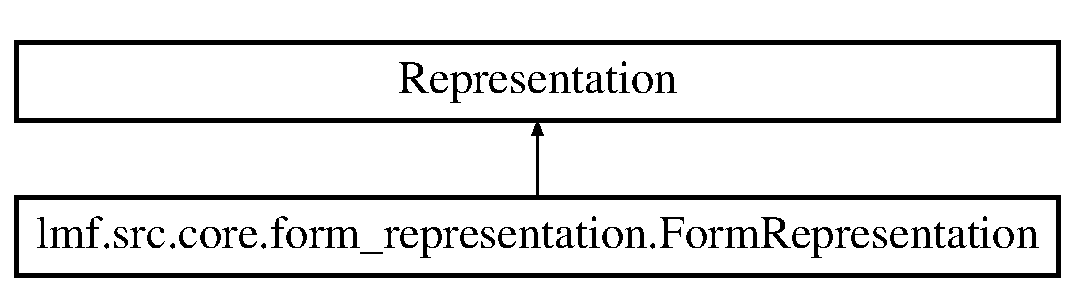
\includegraphics[height=2.000000cm]{classlmf_1_1src_1_1core_1_1form__representation_1_1_form_representation}
\end{center}
\end{figure}
\subsection*{Public Member Functions}
\begin{DoxyCompactItemize}
\item 
def \hyperlink{classlmf_1_1src_1_1core_1_1form__representation_1_1_form_representation_ab034318ab1492fac033d745860e18a37}{\+\_\+\+\_\+init\+\_\+\+\_\+}
\begin{DoxyCompactList}\small\item\em Constructor. \end{DoxyCompactList}\item 
def \hyperlink{classlmf_1_1src_1_1core_1_1form__representation_1_1_form_representation_a577b5258bf8f64ff889f0588cf0c8eda}{\+\_\+\+\_\+del\+\_\+\+\_\+}
\begin{DoxyCompactList}\small\item\em Destructor. \end{DoxyCompactList}\item 
def \hyperlink{classlmf_1_1src_1_1core_1_1form__representation_1_1_form_representation_a348d8eb39ef5bda7789106c9f5fe7755}{get\+\_\+speakers}
\begin{DoxyCompactList}\small\item\em Get speakers. \end{DoxyCompactList}\end{DoxyCompactItemize}
\subsection*{Public Attributes}
\begin{DoxyCompactItemize}
\item 
\hyperlink{classlmf_1_1src_1_1core_1_1form__representation_1_1_form_representation_ab192387108c3c4e780297d1b409d5eff}{transliteration}
\item 
\hyperlink{classlmf_1_1src_1_1core_1_1form__representation_1_1_form_representation_a2cfea0271f8abfcffb74afb7641ef4df}{tone}
\item 
\hyperlink{classlmf_1_1src_1_1core_1_1form__representation_1_1_form_representation_a7d080181b73f2c03d3a2cf65a97be169}{geographical\+Variant}
\item 
\hyperlink{classlmf_1_1src_1_1core_1_1form__representation_1_1_form_representation_a50b914930f083c55e70e805a2430e88d}{phonetic\+Form}
\item 
\hyperlink{classlmf_1_1src_1_1core_1_1form__representation_1_1_form_representation_a1068952fddde59f78e8a56b785b0bcbf}{contextual\+Variation}
\item 
\hyperlink{classlmf_1_1src_1_1core_1_1form__representation_1_1_form_representation_aef2857854ecb2ca02c7ede104b617505}{spelling\+Variant}
\item 
\hyperlink{classlmf_1_1src_1_1core_1_1form__representation_1_1_form_representation_a70151ff258dea274006e4976818847a3}{citation\+Form}
\item 
\hyperlink{classlmf_1_1src_1_1core_1_1form__representation_1_1_form_representation_ad19ad7a519048bc71ff0d0df2c888621}{dialect}
\item 
\hyperlink{classlmf_1_1src_1_1core_1_1form__representation_1_1_form_representation_ad42d4a830850a55fd08ba3742abdde57}{language}
\item 
\hyperlink{classlmf_1_1src_1_1core_1_1form__representation_1_1_form_representation_a728fa20d7dcdbb6714f97b87cbe8ee0f}{script\+Name}
\item 
\hyperlink{classlmf_1_1src_1_1core_1_1form__representation_1_1_form_representation_ac13f0605619b9bdc6b921ae19b39c068}{audio}
\begin{DoxyCompactList}\small\item\em Audio instances are owned by \hyperlink{classlmf_1_1src_1_1core_1_1form__representation_1_1_form_representation}{Form\+Representation} There is zero to many Audio instances per \hyperlink{classlmf_1_1src_1_1core_1_1form__representation_1_1_form_representation}{Form\+Representation}. \end{DoxyCompactList}\item 
\hyperlink{classlmf_1_1src_1_1core_1_1form__representation_1_1_form_representation_a94e0845b7cf84cdbef5f1dceae0d7f99}{targets}
\end{DoxyCompactItemize}


\subsection{Detailed Description}
\char`\"{}\+Form Representation is a class representing one variant orthography of a Form.\char`\"{} (L\+M\+F) 

Definition at line 8 of file form\+\_\+representation.\+py.



\subsection{Constructor \& Destructor Documentation}
\hypertarget{classlmf_1_1src_1_1core_1_1form__representation_1_1_form_representation_ab034318ab1492fac033d745860e18a37}{\index{lmf\+::src\+::core\+::form\+\_\+representation\+::\+Form\+Representation@{lmf\+::src\+::core\+::form\+\_\+representation\+::\+Form\+Representation}!\+\_\+\+\_\+init\+\_\+\+\_\+@{\+\_\+\+\_\+init\+\_\+\+\_\+}}
\index{\+\_\+\+\_\+init\+\_\+\+\_\+@{\+\_\+\+\_\+init\+\_\+\+\_\+}!lmf\+::src\+::core\+::form\+\_\+representation\+::\+Form\+Representation@{lmf\+::src\+::core\+::form\+\_\+representation\+::\+Form\+Representation}}
\subsubsection[{\+\_\+\+\_\+init\+\_\+\+\_\+}]{\setlength{\rightskip}{0pt plus 5cm}def lmf.\+src.\+core.\+form\+\_\+representation.\+Form\+Representation.\+\_\+\+\_\+init\+\_\+\+\_\+ (
\begin{DoxyParamCaption}
\item[{}]{self}
\end{DoxyParamCaption}
)}}\label{classlmf_1_1src_1_1core_1_1form__representation_1_1_form_representation_ab034318ab1492fac033d745860e18a37}


Constructor. 

\hyperlink{classlmf_1_1src_1_1core_1_1form__representation_1_1_form_representation}{Form\+Representation} instances are owned by Form. \begin{DoxyReturn}{Returns}
A \hyperlink{classlmf_1_1src_1_1core_1_1form__representation_1_1_form_representation}{Form\+Representation} instance. 
\end{DoxyReturn}


Definition at line 11 of file form\+\_\+representation.\+py.

\hypertarget{classlmf_1_1src_1_1core_1_1form__representation_1_1_form_representation_a577b5258bf8f64ff889f0588cf0c8eda}{\index{lmf\+::src\+::core\+::form\+\_\+representation\+::\+Form\+Representation@{lmf\+::src\+::core\+::form\+\_\+representation\+::\+Form\+Representation}!\+\_\+\+\_\+del\+\_\+\+\_\+@{\+\_\+\+\_\+del\+\_\+\+\_\+}}
\index{\+\_\+\+\_\+del\+\_\+\+\_\+@{\+\_\+\+\_\+del\+\_\+\+\_\+}!lmf\+::src\+::core\+::form\+\_\+representation\+::\+Form\+Representation@{lmf\+::src\+::core\+::form\+\_\+representation\+::\+Form\+Representation}}
\subsubsection[{\+\_\+\+\_\+del\+\_\+\+\_\+}]{\setlength{\rightskip}{0pt plus 5cm}def lmf.\+src.\+core.\+form\+\_\+representation.\+Form\+Representation.\+\_\+\+\_\+del\+\_\+\+\_\+ (
\begin{DoxyParamCaption}
\item[{}]{self}
\end{DoxyParamCaption}
)}}\label{classlmf_1_1src_1_1core_1_1form__representation_1_1_form_representation_a577b5258bf8f64ff889f0588cf0c8eda}


Destructor. 

Release Audio instances. 

Definition at line 37 of file form\+\_\+representation.\+py.



\subsection{Member Function Documentation}
\hypertarget{classlmf_1_1src_1_1core_1_1form__representation_1_1_form_representation_a348d8eb39ef5bda7789106c9f5fe7755}{\index{lmf\+::src\+::core\+::form\+\_\+representation\+::\+Form\+Representation@{lmf\+::src\+::core\+::form\+\_\+representation\+::\+Form\+Representation}!get\+\_\+speakers@{get\+\_\+speakers}}
\index{get\+\_\+speakers@{get\+\_\+speakers}!lmf\+::src\+::core\+::form\+\_\+representation\+::\+Form\+Representation@{lmf\+::src\+::core\+::form\+\_\+representation\+::\+Form\+Representation}}
\subsubsection[{get\+\_\+speakers}]{\setlength{\rightskip}{0pt plus 5cm}def lmf.\+src.\+core.\+form\+\_\+representation.\+Form\+Representation.\+get\+\_\+speakers (
\begin{DoxyParamCaption}
\item[{}]{self}
\end{DoxyParamCaption}
)}}\label{classlmf_1_1src_1_1core_1_1form__representation_1_1_form_representation_a348d8eb39ef5bda7789106c9f5fe7755}


Get speakers. 

\begin{DoxyReturn}{Returns}
\hyperlink{classlmf_1_1src_1_1core_1_1form__representation_1_1_form_representation}{Form\+Representation} private attribute '\+\_\+\+\_\+speaker', a Python list of Speaker instances. 
\end{DoxyReturn}


Definition at line 47 of file form\+\_\+representation.\+py.



\subsection{Member Data Documentation}
\hypertarget{classlmf_1_1src_1_1core_1_1form__representation_1_1_form_representation_ac13f0605619b9bdc6b921ae19b39c068}{\index{lmf\+::src\+::core\+::form\+\_\+representation\+::\+Form\+Representation@{lmf\+::src\+::core\+::form\+\_\+representation\+::\+Form\+Representation}!audio@{audio}}
\index{audio@{audio}!lmf\+::src\+::core\+::form\+\_\+representation\+::\+Form\+Representation@{lmf\+::src\+::core\+::form\+\_\+representation\+::\+Form\+Representation}}
\subsubsection[{audio}]{\setlength{\rightskip}{0pt plus 5cm}lmf.\+src.\+core.\+form\+\_\+representation.\+Form\+Representation.\+audio}}\label{classlmf_1_1src_1_1core_1_1form__representation_1_1_form_representation_ac13f0605619b9bdc6b921ae19b39c068}


Audio instances are owned by \hyperlink{classlmf_1_1src_1_1core_1_1form__representation_1_1_form_representation}{Form\+Representation} There is zero to many Audio instances per \hyperlink{classlmf_1_1src_1_1core_1_1form__representation_1_1_form_representation}{Form\+Representation}. 



Definition at line 30 of file form\+\_\+representation.\+py.

\hypertarget{classlmf_1_1src_1_1core_1_1form__representation_1_1_form_representation_a70151ff258dea274006e4976818847a3}{\index{lmf\+::src\+::core\+::form\+\_\+representation\+::\+Form\+Representation@{lmf\+::src\+::core\+::form\+\_\+representation\+::\+Form\+Representation}!citation\+Form@{citation\+Form}}
\index{citation\+Form@{citation\+Form}!lmf\+::src\+::core\+::form\+\_\+representation\+::\+Form\+Representation@{lmf\+::src\+::core\+::form\+\_\+representation\+::\+Form\+Representation}}
\subsubsection[{citation\+Form}]{\setlength{\rightskip}{0pt plus 5cm}lmf.\+src.\+core.\+form\+\_\+representation.\+Form\+Representation.\+citation\+Form}}\label{classlmf_1_1src_1_1core_1_1form__representation_1_1_form_representation_a70151ff258dea274006e4976818847a3}


Definition at line 24 of file form\+\_\+representation.\+py.

\hypertarget{classlmf_1_1src_1_1core_1_1form__representation_1_1_form_representation_a1068952fddde59f78e8a56b785b0bcbf}{\index{lmf\+::src\+::core\+::form\+\_\+representation\+::\+Form\+Representation@{lmf\+::src\+::core\+::form\+\_\+representation\+::\+Form\+Representation}!contextual\+Variation@{contextual\+Variation}}
\index{contextual\+Variation@{contextual\+Variation}!lmf\+::src\+::core\+::form\+\_\+representation\+::\+Form\+Representation@{lmf\+::src\+::core\+::form\+\_\+representation\+::\+Form\+Representation}}
\subsubsection[{contextual\+Variation}]{\setlength{\rightskip}{0pt plus 5cm}lmf.\+src.\+core.\+form\+\_\+representation.\+Form\+Representation.\+contextual\+Variation}}\label{classlmf_1_1src_1_1core_1_1form__representation_1_1_form_representation_a1068952fddde59f78e8a56b785b0bcbf}


Definition at line 22 of file form\+\_\+representation.\+py.

\hypertarget{classlmf_1_1src_1_1core_1_1form__representation_1_1_form_representation_ad19ad7a519048bc71ff0d0df2c888621}{\index{lmf\+::src\+::core\+::form\+\_\+representation\+::\+Form\+Representation@{lmf\+::src\+::core\+::form\+\_\+representation\+::\+Form\+Representation}!dialect@{dialect}}
\index{dialect@{dialect}!lmf\+::src\+::core\+::form\+\_\+representation\+::\+Form\+Representation@{lmf\+::src\+::core\+::form\+\_\+representation\+::\+Form\+Representation}}
\subsubsection[{dialect}]{\setlength{\rightskip}{0pt plus 5cm}lmf.\+src.\+core.\+form\+\_\+representation.\+Form\+Representation.\+dialect}}\label{classlmf_1_1src_1_1core_1_1form__representation_1_1_form_representation_ad19ad7a519048bc71ff0d0df2c888621}


Definition at line 25 of file form\+\_\+representation.\+py.

\hypertarget{classlmf_1_1src_1_1core_1_1form__representation_1_1_form_representation_a7d080181b73f2c03d3a2cf65a97be169}{\index{lmf\+::src\+::core\+::form\+\_\+representation\+::\+Form\+Representation@{lmf\+::src\+::core\+::form\+\_\+representation\+::\+Form\+Representation}!geographical\+Variant@{geographical\+Variant}}
\index{geographical\+Variant@{geographical\+Variant}!lmf\+::src\+::core\+::form\+\_\+representation\+::\+Form\+Representation@{lmf\+::src\+::core\+::form\+\_\+representation\+::\+Form\+Representation}}
\subsubsection[{geographical\+Variant}]{\setlength{\rightskip}{0pt plus 5cm}lmf.\+src.\+core.\+form\+\_\+representation.\+Form\+Representation.\+geographical\+Variant}}\label{classlmf_1_1src_1_1core_1_1form__representation_1_1_form_representation_a7d080181b73f2c03d3a2cf65a97be169}


Definition at line 20 of file form\+\_\+representation.\+py.

\hypertarget{classlmf_1_1src_1_1core_1_1form__representation_1_1_form_representation_ad42d4a830850a55fd08ba3742abdde57}{\index{lmf\+::src\+::core\+::form\+\_\+representation\+::\+Form\+Representation@{lmf\+::src\+::core\+::form\+\_\+representation\+::\+Form\+Representation}!language@{language}}
\index{language@{language}!lmf\+::src\+::core\+::form\+\_\+representation\+::\+Form\+Representation@{lmf\+::src\+::core\+::form\+\_\+representation\+::\+Form\+Representation}}
\subsubsection[{language}]{\setlength{\rightskip}{0pt plus 5cm}lmf.\+src.\+core.\+form\+\_\+representation.\+Form\+Representation.\+language}}\label{classlmf_1_1src_1_1core_1_1form__representation_1_1_form_representation_ad42d4a830850a55fd08ba3742abdde57}


Definition at line 26 of file form\+\_\+representation.\+py.

\hypertarget{classlmf_1_1src_1_1core_1_1form__representation_1_1_form_representation_a50b914930f083c55e70e805a2430e88d}{\index{lmf\+::src\+::core\+::form\+\_\+representation\+::\+Form\+Representation@{lmf\+::src\+::core\+::form\+\_\+representation\+::\+Form\+Representation}!phonetic\+Form@{phonetic\+Form}}
\index{phonetic\+Form@{phonetic\+Form}!lmf\+::src\+::core\+::form\+\_\+representation\+::\+Form\+Representation@{lmf\+::src\+::core\+::form\+\_\+representation\+::\+Form\+Representation}}
\subsubsection[{phonetic\+Form}]{\setlength{\rightskip}{0pt plus 5cm}lmf.\+src.\+core.\+form\+\_\+representation.\+Form\+Representation.\+phonetic\+Form}}\label{classlmf_1_1src_1_1core_1_1form__representation_1_1_form_representation_a50b914930f083c55e70e805a2430e88d}


Definition at line 21 of file form\+\_\+representation.\+py.

\hypertarget{classlmf_1_1src_1_1core_1_1form__representation_1_1_form_representation_a728fa20d7dcdbb6714f97b87cbe8ee0f}{\index{lmf\+::src\+::core\+::form\+\_\+representation\+::\+Form\+Representation@{lmf\+::src\+::core\+::form\+\_\+representation\+::\+Form\+Representation}!script\+Name@{script\+Name}}
\index{script\+Name@{script\+Name}!lmf\+::src\+::core\+::form\+\_\+representation\+::\+Form\+Representation@{lmf\+::src\+::core\+::form\+\_\+representation\+::\+Form\+Representation}}
\subsubsection[{script\+Name}]{\setlength{\rightskip}{0pt plus 5cm}lmf.\+src.\+core.\+form\+\_\+representation.\+Form\+Representation.\+script\+Name}}\label{classlmf_1_1src_1_1core_1_1form__representation_1_1_form_representation_a728fa20d7dcdbb6714f97b87cbe8ee0f}


Definition at line 27 of file form\+\_\+representation.\+py.

\hypertarget{classlmf_1_1src_1_1core_1_1form__representation_1_1_form_representation_aef2857854ecb2ca02c7ede104b617505}{\index{lmf\+::src\+::core\+::form\+\_\+representation\+::\+Form\+Representation@{lmf\+::src\+::core\+::form\+\_\+representation\+::\+Form\+Representation}!spelling\+Variant@{spelling\+Variant}}
\index{spelling\+Variant@{spelling\+Variant}!lmf\+::src\+::core\+::form\+\_\+representation\+::\+Form\+Representation@{lmf\+::src\+::core\+::form\+\_\+representation\+::\+Form\+Representation}}
\subsubsection[{spelling\+Variant}]{\setlength{\rightskip}{0pt plus 5cm}lmf.\+src.\+core.\+form\+\_\+representation.\+Form\+Representation.\+spelling\+Variant}}\label{classlmf_1_1src_1_1core_1_1form__representation_1_1_form_representation_aef2857854ecb2ca02c7ede104b617505}


Definition at line 23 of file form\+\_\+representation.\+py.

\hypertarget{classlmf_1_1src_1_1core_1_1form__representation_1_1_form_representation_a94e0845b7cf84cdbef5f1dceae0d7f99}{\index{lmf\+::src\+::core\+::form\+\_\+representation\+::\+Form\+Representation@{lmf\+::src\+::core\+::form\+\_\+representation\+::\+Form\+Representation}!targets@{targets}}
\index{targets@{targets}!lmf\+::src\+::core\+::form\+\_\+representation\+::\+Form\+Representation@{lmf\+::src\+::core\+::form\+\_\+representation\+::\+Form\+Representation}}
\subsubsection[{targets}]{\setlength{\rightskip}{0pt plus 5cm}lmf.\+src.\+core.\+form\+\_\+representation.\+Form\+Representation.\+targets}}\label{classlmf_1_1src_1_1core_1_1form__representation_1_1_form_representation_a94e0845b7cf84cdbef5f1dceae0d7f99}


Definition at line 32 of file form\+\_\+representation.\+py.

\hypertarget{classlmf_1_1src_1_1core_1_1form__representation_1_1_form_representation_a2cfea0271f8abfcffb74afb7641ef4df}{\index{lmf\+::src\+::core\+::form\+\_\+representation\+::\+Form\+Representation@{lmf\+::src\+::core\+::form\+\_\+representation\+::\+Form\+Representation}!tone@{tone}}
\index{tone@{tone}!lmf\+::src\+::core\+::form\+\_\+representation\+::\+Form\+Representation@{lmf\+::src\+::core\+::form\+\_\+representation\+::\+Form\+Representation}}
\subsubsection[{tone}]{\setlength{\rightskip}{0pt plus 5cm}lmf.\+src.\+core.\+form\+\_\+representation.\+Form\+Representation.\+tone}}\label{classlmf_1_1src_1_1core_1_1form__representation_1_1_form_representation_a2cfea0271f8abfcffb74afb7641ef4df}


Definition at line 19 of file form\+\_\+representation.\+py.

\hypertarget{classlmf_1_1src_1_1core_1_1form__representation_1_1_form_representation_ab192387108c3c4e780297d1b409d5eff}{\index{lmf\+::src\+::core\+::form\+\_\+representation\+::\+Form\+Representation@{lmf\+::src\+::core\+::form\+\_\+representation\+::\+Form\+Representation}!transliteration@{transliteration}}
\index{transliteration@{transliteration}!lmf\+::src\+::core\+::form\+\_\+representation\+::\+Form\+Representation@{lmf\+::src\+::core\+::form\+\_\+representation\+::\+Form\+Representation}}
\subsubsection[{transliteration}]{\setlength{\rightskip}{0pt plus 5cm}lmf.\+src.\+core.\+form\+\_\+representation.\+Form\+Representation.\+transliteration}}\label{classlmf_1_1src_1_1core_1_1form__representation_1_1_form_representation_ab192387108c3c4e780297d1b409d5eff}


Definition at line 18 of file form\+\_\+representation.\+py.



The documentation for this class was generated from the following file\+:\begin{DoxyCompactItemize}
\item 
/\+Users/celine/\+Work/\+C\+N\+R\+S/workspace/\+Himal\+Co/dev/lib/lmf/src/core/\hyperlink{form__representation_8py}{form\+\_\+representation.\+py}\end{DoxyCompactItemize}

\hypertarget{classlmf_1_1src_1_1core_1_1global__information_1_1_global_information}{\section{lmf.\+src.\+core.\+global\+\_\+information.\+Global\+Information Class Reference}
\label{classlmf_1_1src_1_1core_1_1global__information_1_1_global_information}\index{lmf.\+src.\+core.\+global\+\_\+information.\+Global\+Information@{lmf.\+src.\+core.\+global\+\_\+information.\+Global\+Information}}
}


\char`\"{}\+Global Information is a class for administrative information and other general attributes, such as /language coding/ or /script coding/, which are valid for the entire lexical resource.\char`\"{} (L\+M\+F)  


\subsection*{Public Member Functions}
\begin{DoxyCompactItemize}
\item 
def \hyperlink{classlmf_1_1src_1_1core_1_1global__information_1_1_global_information_a8815a24e93798f1e253ba79ec38cb30f}{\+\_\+\+\_\+init\+\_\+\+\_\+}
\begin{DoxyCompactList}\small\item\em Constructor. \end{DoxyCompactList}\item 
def \hyperlink{classlmf_1_1src_1_1core_1_1global__information_1_1_global_information_a9ef2d1611e39e6d3802651da2b46ef1c}{\+\_\+\+\_\+del\+\_\+\+\_\+}
\begin{DoxyCompactList}\small\item\em Destructor. \end{DoxyCompactList}\end{DoxyCompactItemize}
\subsection*{Public Attributes}
\begin{DoxyCompactItemize}
\item 
\hyperlink{classlmf_1_1src_1_1core_1_1global__information_1_1_global_information_a13b6750b6876cade278c3cde1f0625a2}{language\+Code}
\item 
\hyperlink{classlmf_1_1src_1_1core_1_1global__information_1_1_global_information_a96ffe5559235b6b6c681b45a61d697af}{author}
\item 
\hyperlink{classlmf_1_1src_1_1core_1_1global__information_1_1_global_information_a6a0bbf60025ea9503bb541a0ffbd514a}{version}
\item 
\hyperlink{classlmf_1_1src_1_1core_1_1global__information_1_1_global_information_a11e84dd6e15ae319bc1427388614eb31}{last\+Update}
\item 
\hyperlink{classlmf_1_1src_1_1core_1_1global__information_1_1_global_information_a1f086ce6c56515e2c6fd853c7007d015}{license}
\item 
\hyperlink{classlmf_1_1src_1_1core_1_1global__information_1_1_global_information_a7fd2e0b92537d9a5d055ef6726617d1e}{character\+Encoding}
\item 
\hyperlink{classlmf_1_1src_1_1core_1_1global__information_1_1_global_information_a53110d17cbf0bfdcb72fb089e648aa70}{date\+Coding}
\item 
\hyperlink{classlmf_1_1src_1_1core_1_1global__information_1_1_global_information_a45c08bbe888ab19297d903a952085c0c}{creation\+Date}
\item 
\hyperlink{classlmf_1_1src_1_1core_1_1global__information_1_1_global_information_ac22ab44249ba844254fcdc84e7f330fc}{project\+Name}
\item 
\hyperlink{classlmf_1_1src_1_1core_1_1global__information_1_1_global_information_aa37acb480d22d4b7c79ece3f04a6e1a2}{description}
\item 
\hyperlink{classlmf_1_1src_1_1core_1_1global__information_1_1_global_information_a02d9de85d8225dc1411986b763df19ab}{bibliographic\+Citation}
\end{DoxyCompactItemize}


\subsection{Detailed Description}
\char`\"{}\+Global Information is a class for administrative information and other general attributes, such as /language coding/ or /script coding/, which are valid for the entire lexical resource.\char`\"{} (L\+M\+F) 

Definition at line 6 of file global\+\_\+information.\+py.



\subsection{Constructor \& Destructor Documentation}
\hypertarget{classlmf_1_1src_1_1core_1_1global__information_1_1_global_information_a8815a24e93798f1e253ba79ec38cb30f}{\index{lmf\+::src\+::core\+::global\+\_\+information\+::\+Global\+Information@{lmf\+::src\+::core\+::global\+\_\+information\+::\+Global\+Information}!\+\_\+\+\_\+init\+\_\+\+\_\+@{\+\_\+\+\_\+init\+\_\+\+\_\+}}
\index{\+\_\+\+\_\+init\+\_\+\+\_\+@{\+\_\+\+\_\+init\+\_\+\+\_\+}!lmf\+::src\+::core\+::global\+\_\+information\+::\+Global\+Information@{lmf\+::src\+::core\+::global\+\_\+information\+::\+Global\+Information}}
\subsubsection[{\+\_\+\+\_\+init\+\_\+\+\_\+}]{\setlength{\rightskip}{0pt plus 5cm}def lmf.\+src.\+core.\+global\+\_\+information.\+Global\+Information.\+\_\+\+\_\+init\+\_\+\+\_\+ (
\begin{DoxyParamCaption}
\item[{}]{self}
\end{DoxyParamCaption}
)}}\label{classlmf_1_1src_1_1core_1_1global__information_1_1_global_information_a8815a24e93798f1e253ba79ec38cb30f}


Constructor. 

\hyperlink{classlmf_1_1src_1_1core_1_1global__information_1_1_global_information}{Global\+Information} instance is owned by Lexical\+Resource. \begin{DoxyReturn}{Returns}
A \hyperlink{classlmf_1_1src_1_1core_1_1global__information_1_1_global_information}{Global\+Information} instance. 
\end{DoxyReturn}


Definition at line 9 of file global\+\_\+information.\+py.

\hypertarget{classlmf_1_1src_1_1core_1_1global__information_1_1_global_information_a9ef2d1611e39e6d3802651da2b46ef1c}{\index{lmf\+::src\+::core\+::global\+\_\+information\+::\+Global\+Information@{lmf\+::src\+::core\+::global\+\_\+information\+::\+Global\+Information}!\+\_\+\+\_\+del\+\_\+\+\_\+@{\+\_\+\+\_\+del\+\_\+\+\_\+}}
\index{\+\_\+\+\_\+del\+\_\+\+\_\+@{\+\_\+\+\_\+del\+\_\+\+\_\+}!lmf\+::src\+::core\+::global\+\_\+information\+::\+Global\+Information@{lmf\+::src\+::core\+::global\+\_\+information\+::\+Global\+Information}}
\subsubsection[{\+\_\+\+\_\+del\+\_\+\+\_\+}]{\setlength{\rightskip}{0pt plus 5cm}def lmf.\+src.\+core.\+global\+\_\+information.\+Global\+Information.\+\_\+\+\_\+del\+\_\+\+\_\+ (
\begin{DoxyParamCaption}
\item[{}]{self}
\end{DoxyParamCaption}
)}}\label{classlmf_1_1src_1_1core_1_1global__information_1_1_global_information_a9ef2d1611e39e6d3802651da2b46ef1c}


Destructor. 



Definition at line 26 of file global\+\_\+information.\+py.



\subsection{Member Data Documentation}
\hypertarget{classlmf_1_1src_1_1core_1_1global__information_1_1_global_information_a96ffe5559235b6b6c681b45a61d697af}{\index{lmf\+::src\+::core\+::global\+\_\+information\+::\+Global\+Information@{lmf\+::src\+::core\+::global\+\_\+information\+::\+Global\+Information}!author@{author}}
\index{author@{author}!lmf\+::src\+::core\+::global\+\_\+information\+::\+Global\+Information@{lmf\+::src\+::core\+::global\+\_\+information\+::\+Global\+Information}}
\subsubsection[{author}]{\setlength{\rightskip}{0pt plus 5cm}lmf.\+src.\+core.\+global\+\_\+information.\+Global\+Information.\+author}}\label{classlmf_1_1src_1_1core_1_1global__information_1_1_global_information_a96ffe5559235b6b6c681b45a61d697af}


Definition at line 15 of file global\+\_\+information.\+py.

\hypertarget{classlmf_1_1src_1_1core_1_1global__information_1_1_global_information_a02d9de85d8225dc1411986b763df19ab}{\index{lmf\+::src\+::core\+::global\+\_\+information\+::\+Global\+Information@{lmf\+::src\+::core\+::global\+\_\+information\+::\+Global\+Information}!bibliographic\+Citation@{bibliographic\+Citation}}
\index{bibliographic\+Citation@{bibliographic\+Citation}!lmf\+::src\+::core\+::global\+\_\+information\+::\+Global\+Information@{lmf\+::src\+::core\+::global\+\_\+information\+::\+Global\+Information}}
\subsubsection[{bibliographic\+Citation}]{\setlength{\rightskip}{0pt plus 5cm}lmf.\+src.\+core.\+global\+\_\+information.\+Global\+Information.\+bibliographic\+Citation}}\label{classlmf_1_1src_1_1core_1_1global__information_1_1_global_information_a02d9de85d8225dc1411986b763df19ab}


Definition at line 24 of file global\+\_\+information.\+py.

\hypertarget{classlmf_1_1src_1_1core_1_1global__information_1_1_global_information_a7fd2e0b92537d9a5d055ef6726617d1e}{\index{lmf\+::src\+::core\+::global\+\_\+information\+::\+Global\+Information@{lmf\+::src\+::core\+::global\+\_\+information\+::\+Global\+Information}!character\+Encoding@{character\+Encoding}}
\index{character\+Encoding@{character\+Encoding}!lmf\+::src\+::core\+::global\+\_\+information\+::\+Global\+Information@{lmf\+::src\+::core\+::global\+\_\+information\+::\+Global\+Information}}
\subsubsection[{character\+Encoding}]{\setlength{\rightskip}{0pt plus 5cm}lmf.\+src.\+core.\+global\+\_\+information.\+Global\+Information.\+character\+Encoding}}\label{classlmf_1_1src_1_1core_1_1global__information_1_1_global_information_a7fd2e0b92537d9a5d055ef6726617d1e}


Definition at line 19 of file global\+\_\+information.\+py.

\hypertarget{classlmf_1_1src_1_1core_1_1global__information_1_1_global_information_a45c08bbe888ab19297d903a952085c0c}{\index{lmf\+::src\+::core\+::global\+\_\+information\+::\+Global\+Information@{lmf\+::src\+::core\+::global\+\_\+information\+::\+Global\+Information}!creation\+Date@{creation\+Date}}
\index{creation\+Date@{creation\+Date}!lmf\+::src\+::core\+::global\+\_\+information\+::\+Global\+Information@{lmf\+::src\+::core\+::global\+\_\+information\+::\+Global\+Information}}
\subsubsection[{creation\+Date}]{\setlength{\rightskip}{0pt plus 5cm}lmf.\+src.\+core.\+global\+\_\+information.\+Global\+Information.\+creation\+Date}}\label{classlmf_1_1src_1_1core_1_1global__information_1_1_global_information_a45c08bbe888ab19297d903a952085c0c}


Definition at line 21 of file global\+\_\+information.\+py.

\hypertarget{classlmf_1_1src_1_1core_1_1global__information_1_1_global_information_a53110d17cbf0bfdcb72fb089e648aa70}{\index{lmf\+::src\+::core\+::global\+\_\+information\+::\+Global\+Information@{lmf\+::src\+::core\+::global\+\_\+information\+::\+Global\+Information}!date\+Coding@{date\+Coding}}
\index{date\+Coding@{date\+Coding}!lmf\+::src\+::core\+::global\+\_\+information\+::\+Global\+Information@{lmf\+::src\+::core\+::global\+\_\+information\+::\+Global\+Information}}
\subsubsection[{date\+Coding}]{\setlength{\rightskip}{0pt plus 5cm}lmf.\+src.\+core.\+global\+\_\+information.\+Global\+Information.\+date\+Coding}}\label{classlmf_1_1src_1_1core_1_1global__information_1_1_global_information_a53110d17cbf0bfdcb72fb089e648aa70}


Definition at line 20 of file global\+\_\+information.\+py.

\hypertarget{classlmf_1_1src_1_1core_1_1global__information_1_1_global_information_aa37acb480d22d4b7c79ece3f04a6e1a2}{\index{lmf\+::src\+::core\+::global\+\_\+information\+::\+Global\+Information@{lmf\+::src\+::core\+::global\+\_\+information\+::\+Global\+Information}!description@{description}}
\index{description@{description}!lmf\+::src\+::core\+::global\+\_\+information\+::\+Global\+Information@{lmf\+::src\+::core\+::global\+\_\+information\+::\+Global\+Information}}
\subsubsection[{description}]{\setlength{\rightskip}{0pt plus 5cm}lmf.\+src.\+core.\+global\+\_\+information.\+Global\+Information.\+description}}\label{classlmf_1_1src_1_1core_1_1global__information_1_1_global_information_aa37acb480d22d4b7c79ece3f04a6e1a2}


Definition at line 23 of file global\+\_\+information.\+py.

\hypertarget{classlmf_1_1src_1_1core_1_1global__information_1_1_global_information_a13b6750b6876cade278c3cde1f0625a2}{\index{lmf\+::src\+::core\+::global\+\_\+information\+::\+Global\+Information@{lmf\+::src\+::core\+::global\+\_\+information\+::\+Global\+Information}!language\+Code@{language\+Code}}
\index{language\+Code@{language\+Code}!lmf\+::src\+::core\+::global\+\_\+information\+::\+Global\+Information@{lmf\+::src\+::core\+::global\+\_\+information\+::\+Global\+Information}}
\subsubsection[{language\+Code}]{\setlength{\rightskip}{0pt plus 5cm}lmf.\+src.\+core.\+global\+\_\+information.\+Global\+Information.\+language\+Code}}\label{classlmf_1_1src_1_1core_1_1global__information_1_1_global_information_a13b6750b6876cade278c3cde1f0625a2}


Definition at line 14 of file global\+\_\+information.\+py.

\hypertarget{classlmf_1_1src_1_1core_1_1global__information_1_1_global_information_a11e84dd6e15ae319bc1427388614eb31}{\index{lmf\+::src\+::core\+::global\+\_\+information\+::\+Global\+Information@{lmf\+::src\+::core\+::global\+\_\+information\+::\+Global\+Information}!last\+Update@{last\+Update}}
\index{last\+Update@{last\+Update}!lmf\+::src\+::core\+::global\+\_\+information\+::\+Global\+Information@{lmf\+::src\+::core\+::global\+\_\+information\+::\+Global\+Information}}
\subsubsection[{last\+Update}]{\setlength{\rightskip}{0pt plus 5cm}lmf.\+src.\+core.\+global\+\_\+information.\+Global\+Information.\+last\+Update}}\label{classlmf_1_1src_1_1core_1_1global__information_1_1_global_information_a11e84dd6e15ae319bc1427388614eb31}


Definition at line 17 of file global\+\_\+information.\+py.

\hypertarget{classlmf_1_1src_1_1core_1_1global__information_1_1_global_information_a1f086ce6c56515e2c6fd853c7007d015}{\index{lmf\+::src\+::core\+::global\+\_\+information\+::\+Global\+Information@{lmf\+::src\+::core\+::global\+\_\+information\+::\+Global\+Information}!license@{license}}
\index{license@{license}!lmf\+::src\+::core\+::global\+\_\+information\+::\+Global\+Information@{lmf\+::src\+::core\+::global\+\_\+information\+::\+Global\+Information}}
\subsubsection[{license}]{\setlength{\rightskip}{0pt plus 5cm}lmf.\+src.\+core.\+global\+\_\+information.\+Global\+Information.\+license}}\label{classlmf_1_1src_1_1core_1_1global__information_1_1_global_information_a1f086ce6c56515e2c6fd853c7007d015}


Definition at line 18 of file global\+\_\+information.\+py.

\hypertarget{classlmf_1_1src_1_1core_1_1global__information_1_1_global_information_ac22ab44249ba844254fcdc84e7f330fc}{\index{lmf\+::src\+::core\+::global\+\_\+information\+::\+Global\+Information@{lmf\+::src\+::core\+::global\+\_\+information\+::\+Global\+Information}!project\+Name@{project\+Name}}
\index{project\+Name@{project\+Name}!lmf\+::src\+::core\+::global\+\_\+information\+::\+Global\+Information@{lmf\+::src\+::core\+::global\+\_\+information\+::\+Global\+Information}}
\subsubsection[{project\+Name}]{\setlength{\rightskip}{0pt plus 5cm}lmf.\+src.\+core.\+global\+\_\+information.\+Global\+Information.\+project\+Name}}\label{classlmf_1_1src_1_1core_1_1global__information_1_1_global_information_ac22ab44249ba844254fcdc84e7f330fc}


Definition at line 22 of file global\+\_\+information.\+py.

\hypertarget{classlmf_1_1src_1_1core_1_1global__information_1_1_global_information_a6a0bbf60025ea9503bb541a0ffbd514a}{\index{lmf\+::src\+::core\+::global\+\_\+information\+::\+Global\+Information@{lmf\+::src\+::core\+::global\+\_\+information\+::\+Global\+Information}!version@{version}}
\index{version@{version}!lmf\+::src\+::core\+::global\+\_\+information\+::\+Global\+Information@{lmf\+::src\+::core\+::global\+\_\+information\+::\+Global\+Information}}
\subsubsection[{version}]{\setlength{\rightskip}{0pt plus 5cm}lmf.\+src.\+core.\+global\+\_\+information.\+Global\+Information.\+version}}\label{classlmf_1_1src_1_1core_1_1global__information_1_1_global_information_a6a0bbf60025ea9503bb541a0ffbd514a}


Definition at line 16 of file global\+\_\+information.\+py.



The documentation for this class was generated from the following file\+:\begin{DoxyCompactItemize}
\item 
/\+Users/celine/\+Work/\+C\+N\+R\+S/workspace/\+Himal\+Co/dev/lib/lmf/src/core/\hyperlink{global__information_8py}{global\+\_\+information.\+py}\end{DoxyCompactItemize}

\hypertarget{classlmf_1_1src_1_1resources_1_1human__resource_1_1_human_resource}{\section{lmf.\+src.\+resources.\+human\+\_\+resource.\+Human\+Resource Class Reference}
\label{classlmf_1_1src_1_1resources_1_1human__resource_1_1_human_resource}\index{lmf.\+src.\+resources.\+human\+\_\+resource.\+Human\+Resource@{lmf.\+src.\+resources.\+human\+\_\+resource.\+Human\+Resource}}
}


\hyperlink{classlmf_1_1src_1_1resources_1_1human__resource_1_1_human_resource}{Human\+Resource} is a Resource subclass.  


Inheritance diagram for lmf.\+src.\+resources.\+human\+\_\+resource.\+Human\+Resource\+:\begin{figure}[H]
\begin{center}
\leavevmode
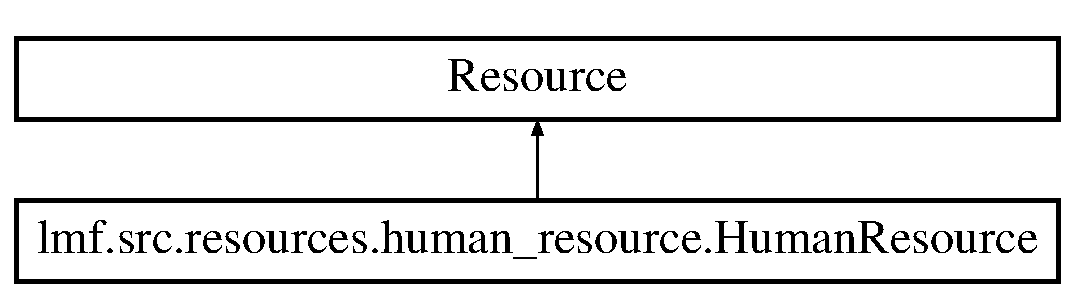
\includegraphics[height=2.000000cm]{classlmf_1_1src_1_1resources_1_1human__resource_1_1_human_resource}
\end{center}
\end{figure}
\subsection*{Public Member Functions}
\begin{DoxyCompactItemize}
\item 
def \hyperlink{classlmf_1_1src_1_1resources_1_1human__resource_1_1_human_resource_a46e116543c9cb199fb4627f25e82a3e1}{\+\_\+\+\_\+init\+\_\+\+\_\+}
\begin{DoxyCompactList}\small\item\em As \hyperlink{classlmf_1_1src_1_1resources_1_1human__resource_1_1_human_resource}{Human\+Resource} is an abstract class, constructor raises an error. \end{DoxyCompactList}\item 
def \hyperlink{classlmf_1_1src_1_1resources_1_1human__resource_1_1_human_resource_a73c9eb976edf10f261b7504e6183319a}{\+\_\+\+\_\+del\+\_\+\+\_\+}
\begin{DoxyCompactList}\small\item\em As \hyperlink{classlmf_1_1src_1_1resources_1_1human__resource_1_1_human_resource}{Human\+Resource} is an abstract class, desctructor raises an error. \end{DoxyCompactList}\item 
def \hyperlink{classlmf_1_1src_1_1resources_1_1human__resource_1_1_human_resource_a091c687c865e89d52ac36b00c1ec32c5}{\+\_\+\+\_\+new\+\_\+\+\_\+}
\begin{DoxyCompactList}\small\item\em Private initialization called from \hyperlink{classlmf_1_1src_1_1resources_1_1human__resource_1_1_human_resource}{Human\+Resource} subclasses. \end{DoxyCompactList}\end{DoxyCompactItemize}
\subsection*{Public Attributes}
\begin{DoxyCompactItemize}
\item 
\hyperlink{classlmf_1_1src_1_1resources_1_1human__resource_1_1_human_resource_a12fcc645b94757742d4ea5c3db0393f0}{name}
\item 
\hyperlink{classlmf_1_1src_1_1resources_1_1human__resource_1_1_human_resource_af75d8c40ab421aea011a028c9ccda753}{anonymization\+Flag}
\item 
\hyperlink{classlmf_1_1src_1_1resources_1_1human__resource_1_1_human_resource_ae236a9203ed63c1afe852eb2708e3949}{reference}
\item 
\hyperlink{classlmf_1_1src_1_1resources_1_1human__resource_1_1_human_resource_a2de15de1c117422bb42047d0f56c796a}{source}
\end{DoxyCompactItemize}


\subsection{Detailed Description}
\hyperlink{classlmf_1_1src_1_1resources_1_1human__resource_1_1_human_resource}{Human\+Resource} is a Resource subclass. 

\hyperlink{classlmf_1_1src_1_1resources_1_1human__resource_1_1_human_resource}{Human\+Resource} is an abstract class representing a speaker. The \hyperlink{classlmf_1_1src_1_1resources_1_1human__resource_1_1_human_resource}{Human\+Resource} class allows subclasses. 

Definition at line 8 of file human\+\_\+resource.\+py.



\subsection{Constructor \& Destructor Documentation}
\hypertarget{classlmf_1_1src_1_1resources_1_1human__resource_1_1_human_resource_a46e116543c9cb199fb4627f25e82a3e1}{\index{lmf\+::src\+::resources\+::human\+\_\+resource\+::\+Human\+Resource@{lmf\+::src\+::resources\+::human\+\_\+resource\+::\+Human\+Resource}!\+\_\+\+\_\+init\+\_\+\+\_\+@{\+\_\+\+\_\+init\+\_\+\+\_\+}}
\index{\+\_\+\+\_\+init\+\_\+\+\_\+@{\+\_\+\+\_\+init\+\_\+\+\_\+}!lmf\+::src\+::resources\+::human\+\_\+resource\+::\+Human\+Resource@{lmf\+::src\+::resources\+::human\+\_\+resource\+::\+Human\+Resource}}
\subsubsection[{\+\_\+\+\_\+init\+\_\+\+\_\+}]{\setlength{\rightskip}{0pt plus 5cm}def lmf.\+src.\+resources.\+human\+\_\+resource.\+Human\+Resource.\+\_\+\+\_\+init\+\_\+\+\_\+ (
\begin{DoxyParamCaption}
\item[{}]{self}
\end{DoxyParamCaption}
)}}\label{classlmf_1_1src_1_1resources_1_1human__resource_1_1_human_resource_a46e116543c9cb199fb4627f25e82a3e1}


As \hyperlink{classlmf_1_1src_1_1resources_1_1human__resource_1_1_human_resource}{Human\+Resource} is an abstract class, constructor raises an error. 



Definition at line 11 of file human\+\_\+resource.\+py.

\hypertarget{classlmf_1_1src_1_1resources_1_1human__resource_1_1_human_resource_a73c9eb976edf10f261b7504e6183319a}{\index{lmf\+::src\+::resources\+::human\+\_\+resource\+::\+Human\+Resource@{lmf\+::src\+::resources\+::human\+\_\+resource\+::\+Human\+Resource}!\+\_\+\+\_\+del\+\_\+\+\_\+@{\+\_\+\+\_\+del\+\_\+\+\_\+}}
\index{\+\_\+\+\_\+del\+\_\+\+\_\+@{\+\_\+\+\_\+del\+\_\+\+\_\+}!lmf\+::src\+::resources\+::human\+\_\+resource\+::\+Human\+Resource@{lmf\+::src\+::resources\+::human\+\_\+resource\+::\+Human\+Resource}}
\subsubsection[{\+\_\+\+\_\+del\+\_\+\+\_\+}]{\setlength{\rightskip}{0pt plus 5cm}def lmf.\+src.\+resources.\+human\+\_\+resource.\+Human\+Resource.\+\_\+\+\_\+del\+\_\+\+\_\+ (
\begin{DoxyParamCaption}
\item[{}]{self}
\end{DoxyParamCaption}
)}}\label{classlmf_1_1src_1_1resources_1_1human__resource_1_1_human_resource_a73c9eb976edf10f261b7504e6183319a}


As \hyperlink{classlmf_1_1src_1_1resources_1_1human__resource_1_1_human_resource}{Human\+Resource} is an abstract class, desctructor raises an error. 



Definition at line 16 of file human\+\_\+resource.\+py.



\subsection{Member Function Documentation}
\hypertarget{classlmf_1_1src_1_1resources_1_1human__resource_1_1_human_resource_a091c687c865e89d52ac36b00c1ec32c5}{\index{lmf\+::src\+::resources\+::human\+\_\+resource\+::\+Human\+Resource@{lmf\+::src\+::resources\+::human\+\_\+resource\+::\+Human\+Resource}!\+\_\+\+\_\+new\+\_\+\+\_\+@{\+\_\+\+\_\+new\+\_\+\+\_\+}}
\index{\+\_\+\+\_\+new\+\_\+\+\_\+@{\+\_\+\+\_\+new\+\_\+\+\_\+}!lmf\+::src\+::resources\+::human\+\_\+resource\+::\+Human\+Resource@{lmf\+::src\+::resources\+::human\+\_\+resource\+::\+Human\+Resource}}
\subsubsection[{\+\_\+\+\_\+new\+\_\+\+\_\+}]{\setlength{\rightskip}{0pt plus 5cm}def lmf.\+src.\+resources.\+human\+\_\+resource.\+Human\+Resource.\+\_\+\+\_\+new\+\_\+\+\_\+ (
\begin{DoxyParamCaption}
\item[{}]{self}
\end{DoxyParamCaption}
)}}\label{classlmf_1_1src_1_1resources_1_1human__resource_1_1_human_resource_a091c687c865e89d52ac36b00c1ec32c5}


Private initialization called from \hyperlink{classlmf_1_1src_1_1resources_1_1human__resource_1_1_human_resource}{Human\+Resource} subclasses. 

\hyperlink{classlmf_1_1src_1_1resources_1_1human__resource_1_1_human_resource}{Human\+Resource} subinstances are owned by Lexical\+Resource. 

Definition at line 21 of file human\+\_\+resource.\+py.



\subsection{Member Data Documentation}
\hypertarget{classlmf_1_1src_1_1resources_1_1human__resource_1_1_human_resource_af75d8c40ab421aea011a028c9ccda753}{\index{lmf\+::src\+::resources\+::human\+\_\+resource\+::\+Human\+Resource@{lmf\+::src\+::resources\+::human\+\_\+resource\+::\+Human\+Resource}!anonymization\+Flag@{anonymization\+Flag}}
\index{anonymization\+Flag@{anonymization\+Flag}!lmf\+::src\+::resources\+::human\+\_\+resource\+::\+Human\+Resource@{lmf\+::src\+::resources\+::human\+\_\+resource\+::\+Human\+Resource}}
\subsubsection[{anonymization\+Flag}]{\setlength{\rightskip}{0pt plus 5cm}lmf.\+src.\+resources.\+human\+\_\+resource.\+Human\+Resource.\+anonymization\+Flag}}\label{classlmf_1_1src_1_1resources_1_1human__resource_1_1_human_resource_af75d8c40ab421aea011a028c9ccda753}


Definition at line 26 of file human\+\_\+resource.\+py.

\hypertarget{classlmf_1_1src_1_1resources_1_1human__resource_1_1_human_resource_a12fcc645b94757742d4ea5c3db0393f0}{\index{lmf\+::src\+::resources\+::human\+\_\+resource\+::\+Human\+Resource@{lmf\+::src\+::resources\+::human\+\_\+resource\+::\+Human\+Resource}!name@{name}}
\index{name@{name}!lmf\+::src\+::resources\+::human\+\_\+resource\+::\+Human\+Resource@{lmf\+::src\+::resources\+::human\+\_\+resource\+::\+Human\+Resource}}
\subsubsection[{name}]{\setlength{\rightskip}{0pt plus 5cm}lmf.\+src.\+resources.\+human\+\_\+resource.\+Human\+Resource.\+name}}\label{classlmf_1_1src_1_1resources_1_1human__resource_1_1_human_resource_a12fcc645b94757742d4ea5c3db0393f0}


Definition at line 25 of file human\+\_\+resource.\+py.

\hypertarget{classlmf_1_1src_1_1resources_1_1human__resource_1_1_human_resource_ae236a9203ed63c1afe852eb2708e3949}{\index{lmf\+::src\+::resources\+::human\+\_\+resource\+::\+Human\+Resource@{lmf\+::src\+::resources\+::human\+\_\+resource\+::\+Human\+Resource}!reference@{reference}}
\index{reference@{reference}!lmf\+::src\+::resources\+::human\+\_\+resource\+::\+Human\+Resource@{lmf\+::src\+::resources\+::human\+\_\+resource\+::\+Human\+Resource}}
\subsubsection[{reference}]{\setlength{\rightskip}{0pt plus 5cm}lmf.\+src.\+resources.\+human\+\_\+resource.\+Human\+Resource.\+reference}}\label{classlmf_1_1src_1_1resources_1_1human__resource_1_1_human_resource_ae236a9203ed63c1afe852eb2708e3949}


Definition at line 27 of file human\+\_\+resource.\+py.

\hypertarget{classlmf_1_1src_1_1resources_1_1human__resource_1_1_human_resource_a2de15de1c117422bb42047d0f56c796a}{\index{lmf\+::src\+::resources\+::human\+\_\+resource\+::\+Human\+Resource@{lmf\+::src\+::resources\+::human\+\_\+resource\+::\+Human\+Resource}!source@{source}}
\index{source@{source}!lmf\+::src\+::resources\+::human\+\_\+resource\+::\+Human\+Resource@{lmf\+::src\+::resources\+::human\+\_\+resource\+::\+Human\+Resource}}
\subsubsection[{source}]{\setlength{\rightskip}{0pt plus 5cm}lmf.\+src.\+resources.\+human\+\_\+resource.\+Human\+Resource.\+source}}\label{classlmf_1_1src_1_1resources_1_1human__resource_1_1_human_resource_a2de15de1c117422bb42047d0f56c796a}


Definition at line 28 of file human\+\_\+resource.\+py.



The documentation for this class was generated from the following file\+:\begin{DoxyCompactItemize}
\item 
/\+Users/celine/\+Work/\+C\+N\+R\+S/workspace/\+Himal\+Co/dev/lib/lmf/src/resources/\hyperlink{human__resource_8py}{human\+\_\+resource.\+py}\end{DoxyCompactItemize}

\hypertarget{classlmf_1_1src_1_1utils_1_1error__handling_1_1_input_error}{\section{lmf.\+src.\+utils.\+error\+\_\+handling.\+Input\+Error Class Reference}
\label{classlmf_1_1src_1_1utils_1_1error__handling_1_1_input_error}\index{lmf.\+src.\+utils.\+error\+\_\+handling.\+Input\+Error@{lmf.\+src.\+utils.\+error\+\_\+handling.\+Input\+Error}}
}


Exception raised for errors in the input.  


Inheritance diagram for lmf.\+src.\+utils.\+error\+\_\+handling.\+Input\+Error\+:\begin{figure}[H]
\begin{center}
\leavevmode
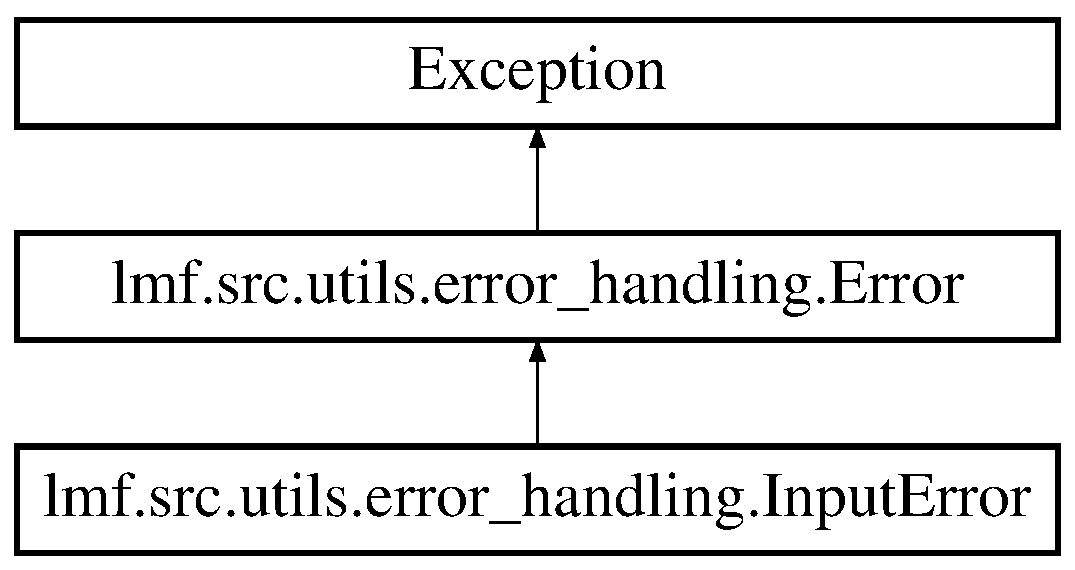
\includegraphics[height=3.000000cm]{classlmf_1_1src_1_1utils_1_1error__handling_1_1_input_error}
\end{center}
\end{figure}
\subsection*{Public Member Functions}
\begin{DoxyCompactItemize}
\item 
def \hyperlink{classlmf_1_1src_1_1utils_1_1error__handling_1_1_input_error_ac78b36781ea6b31a7c9c7e576c701a5f}{\+\_\+\+\_\+init\+\_\+\+\_\+}
\begin{DoxyCompactList}\small\item\em Constructor. \end{DoxyCompactList}\item 
def \hyperlink{classlmf_1_1src_1_1utils_1_1error__handling_1_1_input_error_aacc052f82e4982bfe41d6589a7a249d9}{handle}
\begin{DoxyCompactList}\small\item\em Define behavior to follow in case this error is caught\+: display error and exit program. \end{DoxyCompactList}\end{DoxyCompactItemize}
\subsection*{Public Attributes}
\begin{DoxyCompactItemize}
\item 
\hyperlink{classlmf_1_1src_1_1utils_1_1error__handling_1_1_input_error_a13dc7af38c991d10bbf04900ecc4a44b}{msg}
\item 
\hyperlink{classlmf_1_1src_1_1utils_1_1error__handling_1_1_input_error_a315f51b60727d5ff945e0017a9838e43}{expr}
\item 
\hyperlink{classlmf_1_1src_1_1utils_1_1error__handling_1_1_input_error_a41ac62579b8419be8fee90ac0b907817}{frame\+\_\+info}
\end{DoxyCompactItemize}


\subsection{Detailed Description}
Exception raised for errors in the input. 

Definition at line 41 of file error\+\_\+handling.\+py.



\subsection{Constructor \& Destructor Documentation}
\hypertarget{classlmf_1_1src_1_1utils_1_1error__handling_1_1_input_error_ac78b36781ea6b31a7c9c7e576c701a5f}{\index{lmf\+::src\+::utils\+::error\+\_\+handling\+::\+Input\+Error@{lmf\+::src\+::utils\+::error\+\_\+handling\+::\+Input\+Error}!\+\_\+\+\_\+init\+\_\+\+\_\+@{\+\_\+\+\_\+init\+\_\+\+\_\+}}
\index{\+\_\+\+\_\+init\+\_\+\+\_\+@{\+\_\+\+\_\+init\+\_\+\+\_\+}!lmf\+::src\+::utils\+::error\+\_\+handling\+::\+Input\+Error@{lmf\+::src\+::utils\+::error\+\_\+handling\+::\+Input\+Error}}
\subsubsection[{\+\_\+\+\_\+init\+\_\+\+\_\+}]{\setlength{\rightskip}{0pt plus 5cm}def lmf.\+src.\+utils.\+error\+\_\+handling.\+Input\+Error.\+\_\+\+\_\+init\+\_\+\+\_\+ (
\begin{DoxyParamCaption}
\item[{}]{self, }
\item[{}]{msg, }
\item[{}]{expr = {\ttfamily None}}
\end{DoxyParamCaption}
)}}\label{classlmf_1_1src_1_1utils_1_1error__handling_1_1_input_error_ac78b36781ea6b31a7c9c7e576c701a5f}


Constructor. 


\begin{DoxyParams}{Parameters}
{\em msg} & Explanation of the error. \\
\hline
{\em expr} & Input expression in which the error occurred. \\
\hline
\end{DoxyParams}
\begin{DoxyReturn}{Returns}
An \hyperlink{classlmf_1_1src_1_1utils_1_1error__handling_1_1_input_error}{Input\+Error} instance. 
\end{DoxyReturn}


Definition at line 44 of file error\+\_\+handling.\+py.



\subsection{Member Function Documentation}
\hypertarget{classlmf_1_1src_1_1utils_1_1error__handling_1_1_input_error_aacc052f82e4982bfe41d6589a7a249d9}{\index{lmf\+::src\+::utils\+::error\+\_\+handling\+::\+Input\+Error@{lmf\+::src\+::utils\+::error\+\_\+handling\+::\+Input\+Error}!handle@{handle}}
\index{handle@{handle}!lmf\+::src\+::utils\+::error\+\_\+handling\+::\+Input\+Error@{lmf\+::src\+::utils\+::error\+\_\+handling\+::\+Input\+Error}}
\subsubsection[{handle}]{\setlength{\rightskip}{0pt plus 5cm}def lmf.\+src.\+utils.\+error\+\_\+handling.\+Input\+Error.\+handle (
\begin{DoxyParamCaption}
\item[{}]{self}
\end{DoxyParamCaption}
)}}\label{classlmf_1_1src_1_1utils_1_1error__handling_1_1_input_error_aacc052f82e4982bfe41d6589a7a249d9}


Define behavior to follow in case this error is caught\+: display error and exit program. 



Definition at line 56 of file error\+\_\+handling.\+py.



\subsection{Member Data Documentation}
\hypertarget{classlmf_1_1src_1_1utils_1_1error__handling_1_1_input_error_a315f51b60727d5ff945e0017a9838e43}{\index{lmf\+::src\+::utils\+::error\+\_\+handling\+::\+Input\+Error@{lmf\+::src\+::utils\+::error\+\_\+handling\+::\+Input\+Error}!expr@{expr}}
\index{expr@{expr}!lmf\+::src\+::utils\+::error\+\_\+handling\+::\+Input\+Error@{lmf\+::src\+::utils\+::error\+\_\+handling\+::\+Input\+Error}}
\subsubsection[{expr}]{\setlength{\rightskip}{0pt plus 5cm}lmf.\+src.\+utils.\+error\+\_\+handling.\+Input\+Error.\+expr}}\label{classlmf_1_1src_1_1utils_1_1error__handling_1_1_input_error_a315f51b60727d5ff945e0017a9838e43}


Definition at line 51 of file error\+\_\+handling.\+py.

\hypertarget{classlmf_1_1src_1_1utils_1_1error__handling_1_1_input_error_a41ac62579b8419be8fee90ac0b907817}{\index{lmf\+::src\+::utils\+::error\+\_\+handling\+::\+Input\+Error@{lmf\+::src\+::utils\+::error\+\_\+handling\+::\+Input\+Error}!frame\+\_\+info@{frame\+\_\+info}}
\index{frame\+\_\+info@{frame\+\_\+info}!lmf\+::src\+::utils\+::error\+\_\+handling\+::\+Input\+Error@{lmf\+::src\+::utils\+::error\+\_\+handling\+::\+Input\+Error}}
\subsubsection[{frame\+\_\+info}]{\setlength{\rightskip}{0pt plus 5cm}lmf.\+src.\+utils.\+error\+\_\+handling.\+Input\+Error.\+frame\+\_\+info}}\label{classlmf_1_1src_1_1utils_1_1error__handling_1_1_input_error_a41ac62579b8419be8fee90ac0b907817}


Definition at line 54 of file error\+\_\+handling.\+py.

\hypertarget{classlmf_1_1src_1_1utils_1_1error__handling_1_1_input_error_a13dc7af38c991d10bbf04900ecc4a44b}{\index{lmf\+::src\+::utils\+::error\+\_\+handling\+::\+Input\+Error@{lmf\+::src\+::utils\+::error\+\_\+handling\+::\+Input\+Error}!msg@{msg}}
\index{msg@{msg}!lmf\+::src\+::utils\+::error\+\_\+handling\+::\+Input\+Error@{lmf\+::src\+::utils\+::error\+\_\+handling\+::\+Input\+Error}}
\subsubsection[{msg}]{\setlength{\rightskip}{0pt plus 5cm}lmf.\+src.\+utils.\+error\+\_\+handling.\+Input\+Error.\+msg}}\label{classlmf_1_1src_1_1utils_1_1error__handling_1_1_input_error_a13dc7af38c991d10bbf04900ecc4a44b}


Definition at line 50 of file error\+\_\+handling.\+py.



The documentation for this class was generated from the following file\+:\begin{DoxyCompactItemize}
\item 
/\+Users/celine/\+Work/\+C\+N\+R\+S/workspace/\+Himal\+Co/dev/lib/lmf/src/utils/\hyperlink{error__handling_8py}{error\+\_\+handling.\+py}\end{DoxyCompactItemize}

\hypertarget{classlmf_1_1src_1_1morphology_1_1lemma_1_1_lemma}{\section{lmf.\+src.\+morphology.\+lemma.\+Lemma Class Reference}
\label{classlmf_1_1src_1_1morphology_1_1lemma_1_1_lemma}\index{lmf.\+src.\+morphology.\+lemma.\+Lemma@{lmf.\+src.\+morphology.\+lemma.\+Lemma}}
}


\char`\"{}\+Lemma is a Form subclass representing a form chosen by convention to designate the Lexical Entry. The lemma is usually equivalent to one of the inflected forms, the root, stem or compound phrase.\char`\"{} (L\+M\+F).  


Inheritance diagram for lmf.\+src.\+morphology.\+lemma.\+Lemma\+:\begin{figure}[H]
\begin{center}
\leavevmode
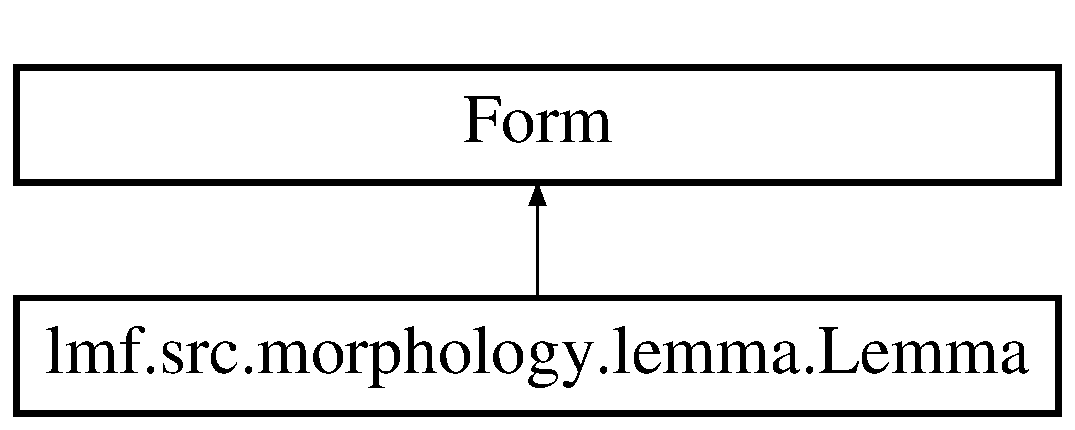
\includegraphics[height=2.000000cm]{classlmf_1_1src_1_1morphology_1_1lemma_1_1_lemma}
\end{center}
\end{figure}
\subsection*{Public Member Functions}
\begin{DoxyCompactItemize}
\item 
def \hyperlink{classlmf_1_1src_1_1morphology_1_1lemma_1_1_lemma_a17223251bd8318631eccd411fbae8115}{\+\_\+\+\_\+init\+\_\+\+\_\+}
\begin{DoxyCompactList}\small\item\em Constructor. \end{DoxyCompactList}\item 
def \hyperlink{classlmf_1_1src_1_1morphology_1_1lemma_1_1_lemma_afd7a268f1743065f5fc3ee53122ea391}{\+\_\+\+\_\+del\+\_\+\+\_\+}
\begin{DoxyCompactList}\small\item\em Destructor. \end{DoxyCompactList}\item 
def \hyperlink{classlmf_1_1src_1_1morphology_1_1lemma_1_1_lemma_a6d6277e8bb71a04cb31aebccd288b6df}{set\+\_\+lexeme}
\begin{DoxyCompactList}\small\item\em Set lexeme. \end{DoxyCompactList}\item 
def \hyperlink{classlmf_1_1src_1_1morphology_1_1lemma_1_1_lemma_ab1bcf9feeb5f59a7c9af07fbc368fb41}{get\+\_\+lexeme}
\begin{DoxyCompactList}\small\item\em Get lexeme. \end{DoxyCompactList}\item 
def \hyperlink{classlmf_1_1src_1_1morphology_1_1lemma_1_1_lemma_a774f121cbc62e3ad4fad738ba8b68da8}{create\+\_\+form\+\_\+representation}
\begin{DoxyCompactList}\small\item\em Create a form representation. \end{DoxyCompactList}\item 
def \hyperlink{classlmf_1_1src_1_1morphology_1_1lemma_1_1_lemma_ab0acb466271ceb0966afbc1c1dc1cdff}{add\+\_\+form\+\_\+representation}
\begin{DoxyCompactList}\small\item\em Add a form representation to the lemma. \end{DoxyCompactList}\item 
def \hyperlink{classlmf_1_1src_1_1morphology_1_1lemma_1_1_lemma_a19275956725afdcfddbbbb491f6783ca}{find\+\_\+form\+\_\+representations}
\begin{DoxyCompactList}\small\item\em Find variant forms. \end{DoxyCompactList}\item 
def \hyperlink{classlmf_1_1src_1_1morphology_1_1lemma_1_1_lemma_aaafc76e4a436188c2ac07417b02e530d}{get\+\_\+form\+\_\+representations}
\begin{DoxyCompactList}\small\item\em Get all form representations maintained by the lemma. \end{DoxyCompactList}\item 
def \hyperlink{classlmf_1_1src_1_1morphology_1_1lemma_1_1_lemma_a71c4c7715794ecd41e5176485f6d7f65}{get\+\_\+form\+\_\+representation}
\begin{DoxyCompactList}\small\item\em Get a given form representation maintained by the lemma. \end{DoxyCompactList}\item 
def \hyperlink{classlmf_1_1src_1_1morphology_1_1lemma_1_1_lemma_a16942d5bd7973fc19eee27a68789dcf5}{set\+\_\+variant\+\_\+form}
\begin{DoxyCompactList}\small\item\em Set variant form and type. \end{DoxyCompactList}\item 
def \hyperlink{classlmf_1_1src_1_1morphology_1_1lemma_1_1_lemma_a6c88624eac96d5660adfda8bf9368164}{get\+\_\+variant\+\_\+forms}
\begin{DoxyCompactList}\small\item\em Get all variant forms of specified type. \end{DoxyCompactList}\item 
def \hyperlink{classlmf_1_1src_1_1morphology_1_1lemma_1_1_lemma_a8d090ef91e9c98ef77d429b3d7296022}{set\+\_\+variant\+\_\+comment}
\begin{DoxyCompactList}\small\item\em Set variant comment and language. \end{DoxyCompactList}\item 
def \hyperlink{classlmf_1_1src_1_1morphology_1_1lemma_1_1_lemma_a094ea5bc786ebf4356bbb1e33c418b92}{set\+\_\+tone}
\begin{DoxyCompactList}\small\item\em Set tone. \end{DoxyCompactList}\item 
def \hyperlink{classlmf_1_1src_1_1morphology_1_1lemma_1_1_lemma_a02afd08362639bdbbac98b35c533375f}{get\+\_\+tones}
\begin{DoxyCompactList}\small\item\em Get all tones. \end{DoxyCompactList}\item 
def \hyperlink{classlmf_1_1src_1_1morphology_1_1lemma_1_1_lemma_a4df66dfca0f2cdf379fa8782d86ba05f}{set\+\_\+geographical\+\_\+variant}
\begin{DoxyCompactList}\small\item\em Set geographical variant. \end{DoxyCompactList}\item 
def \hyperlink{classlmf_1_1src_1_1morphology_1_1lemma_1_1_lemma_ae14b90791332a8d5522ac5056ae2842f}{set\+\_\+phonetic\+\_\+form}
\begin{DoxyCompactList}\small\item\em Set phonetic form. \end{DoxyCompactList}\item 
def \hyperlink{classlmf_1_1src_1_1morphology_1_1lemma_1_1_lemma_af0a2868094d8121b389138319034f164}{get\+\_\+phonetic\+\_\+forms}
\begin{DoxyCompactList}\small\item\em Get all phonetic forms. \end{DoxyCompactList}\item 
def \hyperlink{classlmf_1_1src_1_1morphology_1_1lemma_1_1_lemma_a9f80f34789351b4d3b55c344acb19562}{set\+\_\+contextual\+\_\+variation}
\begin{DoxyCompactList}\small\item\em Set contextual variation. \end{DoxyCompactList}\item 
def \hyperlink{classlmf_1_1src_1_1morphology_1_1lemma_1_1_lemma_a54b9c3f2ae876fdb93b4c4676403c1f0}{get\+\_\+contextual\+\_\+variations}
\begin{DoxyCompactList}\small\item\em Get all contextual variations. \end{DoxyCompactList}\item 
def \hyperlink{classlmf_1_1src_1_1morphology_1_1lemma_1_1_lemma_a01bba6d5da1c9c0d70a3faf762d24f7c}{set\+\_\+spelling\+\_\+variant}
\begin{DoxyCompactList}\small\item\em Set spelling variant. \end{DoxyCompactList}\item 
def \hyperlink{classlmf_1_1src_1_1morphology_1_1lemma_1_1_lemma_a13fb86a829741554939046f500409327}{get\+\_\+spelling\+\_\+variants}
\begin{DoxyCompactList}\small\item\em Get all spelling variants. \end{DoxyCompactList}\item 
def \hyperlink{classlmf_1_1src_1_1morphology_1_1lemma_1_1_lemma_a349b6a8d0a6a571933cd2bede36f695b}{set\+\_\+citation\+\_\+form}
\begin{DoxyCompactList}\small\item\em Set citation form. \end{DoxyCompactList}\item 
def \hyperlink{classlmf_1_1src_1_1morphology_1_1lemma_1_1_lemma_a0d14b66ae5d6f0fd8a9aba74520b88a0}{get\+\_\+citation\+\_\+forms}
\begin{DoxyCompactList}\small\item\em Get all citation forms. \end{DoxyCompactList}\item 
def \hyperlink{classlmf_1_1src_1_1morphology_1_1lemma_1_1_lemma_aa22e9424fc9f35cea9eb1a0a47b3a420}{set\+\_\+dialect}
\begin{DoxyCompactList}\small\item\em Set dialect. \end{DoxyCompactList}\item 
def \hyperlink{classlmf_1_1src_1_1morphology_1_1lemma_1_1_lemma_aa7fbf68d0e986a478493cbf450ae8357}{set\+\_\+transliteration}
\begin{DoxyCompactList}\small\item\em Set transliteration. \end{DoxyCompactList}\item 
def \hyperlink{classlmf_1_1src_1_1morphology_1_1lemma_1_1_lemma_a3e9430de1e0739171a6f655893863708}{get\+\_\+transliterations}
\begin{DoxyCompactList}\small\item\em Get all transliterations. \end{DoxyCompactList}\item 
def \hyperlink{classlmf_1_1src_1_1morphology_1_1lemma_1_1_lemma_aae4244411f218ebc08fc659b1388d7a0}{set\+\_\+script\+\_\+name}
\begin{DoxyCompactList}\small\item\em Set script name. \end{DoxyCompactList}\item 
def \hyperlink{classlmf_1_1src_1_1morphology_1_1lemma_1_1_lemma_abd01bcafb2648b945f049b7852837d67}{set\+\_\+audio}
\begin{DoxyCompactList}\small\item\em Set audio resource. \end{DoxyCompactList}\end{DoxyCompactItemize}
\subsection*{Public Attributes}
\begin{DoxyCompactItemize}
\item 
\hyperlink{classlmf_1_1src_1_1morphology_1_1lemma_1_1_lemma_a225df7c63b5a3a654307bc2d24ed1937}{hyphenation}
\item 
\hyperlink{classlmf_1_1src_1_1morphology_1_1lemma_1_1_lemma_ab68007ef04c51304b92e3eefcf2f40c9}{lexeme}
\end{DoxyCompactItemize}


\subsection{Detailed Description}
\char`\"{}\+Lemma is a Form subclass representing a form chosen by convention to designate the Lexical Entry. The lemma is usually equivalent to one of the inflected forms, the root, stem or compound phrase.\char`\"{} (L\+M\+F). 

Definition at line 9 of file lemma.\+py.



\subsection{Constructor \& Destructor Documentation}
\hypertarget{classlmf_1_1src_1_1morphology_1_1lemma_1_1_lemma_a17223251bd8318631eccd411fbae8115}{\index{lmf\+::src\+::morphology\+::lemma\+::\+Lemma@{lmf\+::src\+::morphology\+::lemma\+::\+Lemma}!\+\_\+\+\_\+init\+\_\+\+\_\+@{\+\_\+\+\_\+init\+\_\+\+\_\+}}
\index{\+\_\+\+\_\+init\+\_\+\+\_\+@{\+\_\+\+\_\+init\+\_\+\+\_\+}!lmf\+::src\+::morphology\+::lemma\+::\+Lemma@{lmf\+::src\+::morphology\+::lemma\+::\+Lemma}}
\subsubsection[{\+\_\+\+\_\+init\+\_\+\+\_\+}]{\setlength{\rightskip}{0pt plus 5cm}def lmf.\+src.\+morphology.\+lemma.\+Lemma.\+\_\+\+\_\+init\+\_\+\+\_\+ (
\begin{DoxyParamCaption}
\item[{}]{self}
\end{DoxyParamCaption}
)}}\label{classlmf_1_1src_1_1morphology_1_1lemma_1_1_lemma_a17223251bd8318631eccd411fbae8115}


Constructor. 

\hyperlink{classlmf_1_1src_1_1morphology_1_1lemma_1_1_lemma}{Lemma} instance is owned by Lexical\+Entry. \begin{DoxyReturn}{Returns}
A \hyperlink{classlmf_1_1src_1_1morphology_1_1lemma_1_1_lemma}{Lemma} instance. 
\end{DoxyReturn}


Definition at line 12 of file lemma.\+py.

\hypertarget{classlmf_1_1src_1_1morphology_1_1lemma_1_1_lemma_afd7a268f1743065f5fc3ee53122ea391}{\index{lmf\+::src\+::morphology\+::lemma\+::\+Lemma@{lmf\+::src\+::morphology\+::lemma\+::\+Lemma}!\+\_\+\+\_\+del\+\_\+\+\_\+@{\+\_\+\+\_\+del\+\_\+\+\_\+}}
\index{\+\_\+\+\_\+del\+\_\+\+\_\+@{\+\_\+\+\_\+del\+\_\+\+\_\+}!lmf\+::src\+::morphology\+::lemma\+::\+Lemma@{lmf\+::src\+::morphology\+::lemma\+::\+Lemma}}
\subsubsection[{\+\_\+\+\_\+del\+\_\+\+\_\+}]{\setlength{\rightskip}{0pt plus 5cm}def lmf.\+src.\+morphology.\+lemma.\+Lemma.\+\_\+\+\_\+del\+\_\+\+\_\+ (
\begin{DoxyParamCaption}
\item[{}]{self}
\end{DoxyParamCaption}
)}}\label{classlmf_1_1src_1_1morphology_1_1lemma_1_1_lemma_afd7a268f1743065f5fc3ee53122ea391}


Destructor. 



Definition at line 22 of file lemma.\+py.



\subsection{Member Function Documentation}
\hypertarget{classlmf_1_1src_1_1morphology_1_1lemma_1_1_lemma_ab0acb466271ceb0966afbc1c1dc1cdff}{\index{lmf\+::src\+::morphology\+::lemma\+::\+Lemma@{lmf\+::src\+::morphology\+::lemma\+::\+Lemma}!add\+\_\+form\+\_\+representation@{add\+\_\+form\+\_\+representation}}
\index{add\+\_\+form\+\_\+representation@{add\+\_\+form\+\_\+representation}!lmf\+::src\+::morphology\+::lemma\+::\+Lemma@{lmf\+::src\+::morphology\+::lemma\+::\+Lemma}}
\subsubsection[{add\+\_\+form\+\_\+representation}]{\setlength{\rightskip}{0pt plus 5cm}def lmf.\+src.\+morphology.\+lemma.\+Lemma.\+add\+\_\+form\+\_\+representation (
\begin{DoxyParamCaption}
\item[{}]{self, }
\item[{}]{form\+\_\+representation}
\end{DoxyParamCaption}
)}}\label{classlmf_1_1src_1_1morphology_1_1lemma_1_1_lemma_ab0acb466271ceb0966afbc1c1dc1cdff}


Add a form representation to the lemma. 


\begin{DoxyParams}{Parameters}
{\em form\+\_\+representation} & The Form\+Representation instance to add to the lemma. \\
\hline
\end{DoxyParams}
\begin{DoxyReturn}{Returns}
\hyperlink{classlmf_1_1src_1_1morphology_1_1lemma_1_1_lemma}{Lemma} instance. 
\end{DoxyReturn}


Definition at line 47 of file lemma.\+py.

\hypertarget{classlmf_1_1src_1_1morphology_1_1lemma_1_1_lemma_a774f121cbc62e3ad4fad738ba8b68da8}{\index{lmf\+::src\+::morphology\+::lemma\+::\+Lemma@{lmf\+::src\+::morphology\+::lemma\+::\+Lemma}!create\+\_\+form\+\_\+representation@{create\+\_\+form\+\_\+representation}}
\index{create\+\_\+form\+\_\+representation@{create\+\_\+form\+\_\+representation}!lmf\+::src\+::morphology\+::lemma\+::\+Lemma@{lmf\+::src\+::morphology\+::lemma\+::\+Lemma}}
\subsubsection[{create\+\_\+form\+\_\+representation}]{\setlength{\rightskip}{0pt plus 5cm}def lmf.\+src.\+morphology.\+lemma.\+Lemma.\+create\+\_\+form\+\_\+representation (
\begin{DoxyParamCaption}
\item[{}]{self}
\end{DoxyParamCaption}
)}}\label{classlmf_1_1src_1_1morphology_1_1lemma_1_1_lemma_a774f121cbc62e3ad4fad738ba8b68da8}


Create a form representation. 

\begin{DoxyReturn}{Returns}
Form\+Representation instance. 
\end{DoxyReturn}


Definition at line 41 of file lemma.\+py.

\hypertarget{classlmf_1_1src_1_1morphology_1_1lemma_1_1_lemma_a19275956725afdcfddbbbb491f6783ca}{\index{lmf\+::src\+::morphology\+::lemma\+::\+Lemma@{lmf\+::src\+::morphology\+::lemma\+::\+Lemma}!find\+\_\+form\+\_\+representations@{find\+\_\+form\+\_\+representations}}
\index{find\+\_\+form\+\_\+representations@{find\+\_\+form\+\_\+representations}!lmf\+::src\+::morphology\+::lemma\+::\+Lemma@{lmf\+::src\+::morphology\+::lemma\+::\+Lemma}}
\subsubsection[{find\+\_\+form\+\_\+representations}]{\setlength{\rightskip}{0pt plus 5cm}def lmf.\+src.\+morphology.\+lemma.\+Lemma.\+find\+\_\+form\+\_\+representations (
\begin{DoxyParamCaption}
\item[{}]{self, }
\item[{}]{type}
\end{DoxyParamCaption}
)}}\label{classlmf_1_1src_1_1morphology_1_1lemma_1_1_lemma_a19275956725afdcfddbbbb491f6783ca}


Find variant forms. 

This attribute is owned by Form\+Representation. 
\begin{DoxyParams}{Parameters}
{\em type} & The type to consider to retrieve the variant form. \\
\hline
\end{DoxyParams}
\begin{DoxyReturn}{Returns}
A Python list of found Form\+Representation attributes 'variant\+Form'. 
\end{DoxyReturn}


Definition at line 55 of file lemma.\+py.

\hypertarget{classlmf_1_1src_1_1morphology_1_1lemma_1_1_lemma_a0d14b66ae5d6f0fd8a9aba74520b88a0}{\index{lmf\+::src\+::morphology\+::lemma\+::\+Lemma@{lmf\+::src\+::morphology\+::lemma\+::\+Lemma}!get\+\_\+citation\+\_\+forms@{get\+\_\+citation\+\_\+forms}}
\index{get\+\_\+citation\+\_\+forms@{get\+\_\+citation\+\_\+forms}!lmf\+::src\+::morphology\+::lemma\+::\+Lemma@{lmf\+::src\+::morphology\+::lemma\+::\+Lemma}}
\subsubsection[{get\+\_\+citation\+\_\+forms}]{\setlength{\rightskip}{0pt plus 5cm}def lmf.\+src.\+morphology.\+lemma.\+Lemma.\+get\+\_\+citation\+\_\+forms (
\begin{DoxyParamCaption}
\item[{}]{self, }
\item[{}]{script\+\_\+name = {\ttfamily None}}
\end{DoxyParamCaption}
)}}\label{classlmf_1_1src_1_1morphology_1_1lemma_1_1_lemma_a0d14b66ae5d6f0fd8a9aba74520b88a0}


Get all citation forms. 

This attribute is owned by Form\+Representation. 
\begin{DoxyParams}{Parameters}
{\em script\+\_\+name} & If provided, get only citation forms that are written using this script. \\
\hline
\end{DoxyParams}
\begin{DoxyReturn}{Returns}
A Python list of Form\+Representation attributes 'citation\+Form'. 
\end{DoxyReturn}


Definition at line 299 of file lemma.\+py.

\hypertarget{classlmf_1_1src_1_1morphology_1_1lemma_1_1_lemma_a54b9c3f2ae876fdb93b4c4676403c1f0}{\index{lmf\+::src\+::morphology\+::lemma\+::\+Lemma@{lmf\+::src\+::morphology\+::lemma\+::\+Lemma}!get\+\_\+contextual\+\_\+variations@{get\+\_\+contextual\+\_\+variations}}
\index{get\+\_\+contextual\+\_\+variations@{get\+\_\+contextual\+\_\+variations}!lmf\+::src\+::morphology\+::lemma\+::\+Lemma@{lmf\+::src\+::morphology\+::lemma\+::\+Lemma}}
\subsubsection[{get\+\_\+contextual\+\_\+variations}]{\setlength{\rightskip}{0pt plus 5cm}def lmf.\+src.\+morphology.\+lemma.\+Lemma.\+get\+\_\+contextual\+\_\+variations (
\begin{DoxyParamCaption}
\item[{}]{self}
\end{DoxyParamCaption}
)}}\label{classlmf_1_1src_1_1morphology_1_1lemma_1_1_lemma_a54b9c3f2ae876fdb93b4c4676403c1f0}


Get all contextual variations. 

This attribute is owned by Form\+Representation. \begin{DoxyReturn}{Returns}
A Python list of Form\+Representation attributes 'contextual\+Variation'. 
\end{DoxyReturn}


Definition at line 236 of file lemma.\+py.

\hypertarget{classlmf_1_1src_1_1morphology_1_1lemma_1_1_lemma_a71c4c7715794ecd41e5176485f6d7f65}{\index{lmf\+::src\+::morphology\+::lemma\+::\+Lemma@{lmf\+::src\+::morphology\+::lemma\+::\+Lemma}!get\+\_\+form\+\_\+representation@{get\+\_\+form\+\_\+representation}}
\index{get\+\_\+form\+\_\+representation@{get\+\_\+form\+\_\+representation}!lmf\+::src\+::morphology\+::lemma\+::\+Lemma@{lmf\+::src\+::morphology\+::lemma\+::\+Lemma}}
\subsubsection[{get\+\_\+form\+\_\+representation}]{\setlength{\rightskip}{0pt plus 5cm}def lmf.\+src.\+morphology.\+lemma.\+Lemma.\+get\+\_\+form\+\_\+representation (
\begin{DoxyParamCaption}
\item[{}]{self, }
\item[{}]{index}
\end{DoxyParamCaption}
)}}\label{classlmf_1_1src_1_1morphology_1_1lemma_1_1_lemma_a71c4c7715794ecd41e5176485f6d7f65}


Get a given form representation maintained by the lemma. 


\begin{DoxyParams}{Parameters}
{\em index} & The index of the wanted form representation. \\
\hline
\end{DoxyParams}
\begin{DoxyReturn}{Returns}
The wanted Form\+Representation instance. 
\end{DoxyReturn}


Definition at line 73 of file lemma.\+py.

\hypertarget{classlmf_1_1src_1_1morphology_1_1lemma_1_1_lemma_aaafc76e4a436188c2ac07417b02e530d}{\index{lmf\+::src\+::morphology\+::lemma\+::\+Lemma@{lmf\+::src\+::morphology\+::lemma\+::\+Lemma}!get\+\_\+form\+\_\+representations@{get\+\_\+form\+\_\+representations}}
\index{get\+\_\+form\+\_\+representations@{get\+\_\+form\+\_\+representations}!lmf\+::src\+::morphology\+::lemma\+::\+Lemma@{lmf\+::src\+::morphology\+::lemma\+::\+Lemma}}
\subsubsection[{get\+\_\+form\+\_\+representations}]{\setlength{\rightskip}{0pt plus 5cm}def lmf.\+src.\+morphology.\+lemma.\+Lemma.\+get\+\_\+form\+\_\+representations (
\begin{DoxyParamCaption}
\item[{}]{self}
\end{DoxyParamCaption}
)}}\label{classlmf_1_1src_1_1morphology_1_1lemma_1_1_lemma_aaafc76e4a436188c2ac07417b02e530d}


Get all form representations maintained by the lemma. 

\begin{DoxyReturn}{Returns}
A Python list of form representations. 
\end{DoxyReturn}


Definition at line 67 of file lemma.\+py.

\hypertarget{classlmf_1_1src_1_1morphology_1_1lemma_1_1_lemma_ab1bcf9feeb5f59a7c9af07fbc368fb41}{\index{lmf\+::src\+::morphology\+::lemma\+::\+Lemma@{lmf\+::src\+::morphology\+::lemma\+::\+Lemma}!get\+\_\+lexeme@{get\+\_\+lexeme}}
\index{get\+\_\+lexeme@{get\+\_\+lexeme}!lmf\+::src\+::morphology\+::lemma\+::\+Lemma@{lmf\+::src\+::morphology\+::lemma\+::\+Lemma}}
\subsubsection[{get\+\_\+lexeme}]{\setlength{\rightskip}{0pt plus 5cm}def lmf.\+src.\+morphology.\+lemma.\+Lemma.\+get\+\_\+lexeme (
\begin{DoxyParamCaption}
\item[{}]{self}
\end{DoxyParamCaption}
)}}\label{classlmf_1_1src_1_1morphology_1_1lemma_1_1_lemma_ab1bcf9feeb5f59a7c9af07fbc368fb41}


Get lexeme. 

\begin{DoxyReturn}{Returns}
\hyperlink{classlmf_1_1src_1_1morphology_1_1lemma_1_1_lemma}{Lemma} attribute 'lexeme'. 
\end{DoxyReturn}


Definition at line 35 of file lemma.\+py.

\hypertarget{classlmf_1_1src_1_1morphology_1_1lemma_1_1_lemma_af0a2868094d8121b389138319034f164}{\index{lmf\+::src\+::morphology\+::lemma\+::\+Lemma@{lmf\+::src\+::morphology\+::lemma\+::\+Lemma}!get\+\_\+phonetic\+\_\+forms@{get\+\_\+phonetic\+\_\+forms}}
\index{get\+\_\+phonetic\+\_\+forms@{get\+\_\+phonetic\+\_\+forms}!lmf\+::src\+::morphology\+::lemma\+::\+Lemma@{lmf\+::src\+::morphology\+::lemma\+::\+Lemma}}
\subsubsection[{get\+\_\+phonetic\+\_\+forms}]{\setlength{\rightskip}{0pt plus 5cm}def lmf.\+src.\+morphology.\+lemma.\+Lemma.\+get\+\_\+phonetic\+\_\+forms (
\begin{DoxyParamCaption}
\item[{}]{self, }
\item[{}]{script\+\_\+name = {\ttfamily None}}
\end{DoxyParamCaption}
)}}\label{classlmf_1_1src_1_1morphology_1_1lemma_1_1_lemma_af0a2868094d8121b389138319034f164}


Get all phonetic forms. 

This attribute is owned by Form\+Representation. 
\begin{DoxyParams}{Parameters}
{\em script\+\_\+name} & If provided, get only phonetic forms that are written using this script. \\
\hline
\end{DoxyParams}
\begin{DoxyReturn}{Returns}
A Python list of Form\+Representation attributes 'phonetic\+Form'. 
\end{DoxyReturn}


Definition at line 205 of file lemma.\+py.

\hypertarget{classlmf_1_1src_1_1morphology_1_1lemma_1_1_lemma_a13fb86a829741554939046f500409327}{\index{lmf\+::src\+::morphology\+::lemma\+::\+Lemma@{lmf\+::src\+::morphology\+::lemma\+::\+Lemma}!get\+\_\+spelling\+\_\+variants@{get\+\_\+spelling\+\_\+variants}}
\index{get\+\_\+spelling\+\_\+variants@{get\+\_\+spelling\+\_\+variants}!lmf\+::src\+::morphology\+::lemma\+::\+Lemma@{lmf\+::src\+::morphology\+::lemma\+::\+Lemma}}
\subsubsection[{get\+\_\+spelling\+\_\+variants}]{\setlength{\rightskip}{0pt plus 5cm}def lmf.\+src.\+morphology.\+lemma.\+Lemma.\+get\+\_\+spelling\+\_\+variants (
\begin{DoxyParamCaption}
\item[{}]{self}
\end{DoxyParamCaption}
)}}\label{classlmf_1_1src_1_1morphology_1_1lemma_1_1_lemma_a13fb86a829741554939046f500409327}


Get all spelling variants. 

This attribute is owned by Form\+Representation. \begin{DoxyReturn}{Returns}
A Python list of Form\+Representation attributes 'spelling\+Variant'. 
\end{DoxyReturn}


Definition at line 266 of file lemma.\+py.

\hypertarget{classlmf_1_1src_1_1morphology_1_1lemma_1_1_lemma_a02afd08362639bdbbac98b35c533375f}{\index{lmf\+::src\+::morphology\+::lemma\+::\+Lemma@{lmf\+::src\+::morphology\+::lemma\+::\+Lemma}!get\+\_\+tones@{get\+\_\+tones}}
\index{get\+\_\+tones@{get\+\_\+tones}!lmf\+::src\+::morphology\+::lemma\+::\+Lemma@{lmf\+::src\+::morphology\+::lemma\+::\+Lemma}}
\subsubsection[{get\+\_\+tones}]{\setlength{\rightskip}{0pt plus 5cm}def lmf.\+src.\+morphology.\+lemma.\+Lemma.\+get\+\_\+tones (
\begin{DoxyParamCaption}
\item[{}]{self}
\end{DoxyParamCaption}
)}}\label{classlmf_1_1src_1_1morphology_1_1lemma_1_1_lemma_a02afd08362639bdbbac98b35c533375f}


Get all tones. 

This attribute is owned by Form\+Representation. \begin{DoxyReturn}{Returns}
A Python list of Form\+Representation attributes 'tone'. 
\end{DoxyReturn}


Definition at line 153 of file lemma.\+py.

\hypertarget{classlmf_1_1src_1_1morphology_1_1lemma_1_1_lemma_a3e9430de1e0739171a6f655893863708}{\index{lmf\+::src\+::morphology\+::lemma\+::\+Lemma@{lmf\+::src\+::morphology\+::lemma\+::\+Lemma}!get\+\_\+transliterations@{get\+\_\+transliterations}}
\index{get\+\_\+transliterations@{get\+\_\+transliterations}!lmf\+::src\+::morphology\+::lemma\+::\+Lemma@{lmf\+::src\+::morphology\+::lemma\+::\+Lemma}}
\subsubsection[{get\+\_\+transliterations}]{\setlength{\rightskip}{0pt plus 5cm}def lmf.\+src.\+morphology.\+lemma.\+Lemma.\+get\+\_\+transliterations (
\begin{DoxyParamCaption}
\item[{}]{self}
\end{DoxyParamCaption}
)}}\label{classlmf_1_1src_1_1morphology_1_1lemma_1_1_lemma_a3e9430de1e0739171a6f655893863708}


Get all transliterations. 

This attribute is owned by Form\+Representation. \begin{DoxyReturn}{Returns}
A Python list of Form\+Representation attributes 'transliteration'. 
\end{DoxyReturn}


Definition at line 349 of file lemma.\+py.

\hypertarget{classlmf_1_1src_1_1morphology_1_1lemma_1_1_lemma_a6c88624eac96d5660adfda8bf9368164}{\index{lmf\+::src\+::morphology\+::lemma\+::\+Lemma@{lmf\+::src\+::morphology\+::lemma\+::\+Lemma}!get\+\_\+variant\+\_\+forms@{get\+\_\+variant\+\_\+forms}}
\index{get\+\_\+variant\+\_\+forms@{get\+\_\+variant\+\_\+forms}!lmf\+::src\+::morphology\+::lemma\+::\+Lemma@{lmf\+::src\+::morphology\+::lemma\+::\+Lemma}}
\subsubsection[{get\+\_\+variant\+\_\+forms}]{\setlength{\rightskip}{0pt plus 5cm}def lmf.\+src.\+morphology.\+lemma.\+Lemma.\+get\+\_\+variant\+\_\+forms (
\begin{DoxyParamCaption}
\item[{}]{self, }
\item[{}]{type = {\ttfamily \char`\"{}unspecified\char`\"{}}}
\end{DoxyParamCaption}
)}}\label{classlmf_1_1src_1_1morphology_1_1lemma_1_1_lemma_a6c88624eac96d5660adfda8bf9368164}


Get all variant forms of specified type. 

This attribute is owned by Form\+Representation. \begin{DoxyReturn}{Returns}
A Python list of Form\+Representation attributes 'variant\+Form' if type matches. 
\end{DoxyReturn}


Definition at line 103 of file lemma.\+py.

\hypertarget{classlmf_1_1src_1_1morphology_1_1lemma_1_1_lemma_abd01bcafb2648b945f049b7852837d67}{\index{lmf\+::src\+::morphology\+::lemma\+::\+Lemma@{lmf\+::src\+::morphology\+::lemma\+::\+Lemma}!set\+\_\+audio@{set\+\_\+audio}}
\index{set\+\_\+audio@{set\+\_\+audio}!lmf\+::src\+::morphology\+::lemma\+::\+Lemma@{lmf\+::src\+::morphology\+::lemma\+::\+Lemma}}
\subsubsection[{set\+\_\+audio}]{\setlength{\rightskip}{0pt plus 5cm}def lmf.\+src.\+morphology.\+lemma.\+Lemma.\+set\+\_\+audio (
\begin{DoxyParamCaption}
\item[{}]{self, }
\item[{}]{media\+\_\+type, }
\item[{}]{file\+\_\+name, }
\item[{}]{author, }
\item[{}]{quality, }
\item[{}]{start\+\_\+position, }
\item[{}]{duration, }
\item[{}]{external\+\_\+reference, }
\item[{}]{audio\+\_\+file\+\_\+format}
\end{DoxyParamCaption}
)}}\label{classlmf_1_1src_1_1morphology_1_1lemma_1_1_lemma_abd01bcafb2648b945f049b7852837d67}


Set audio resource. 

Attributes 'media\+Type', 'file\+Name', 'author', 'quality', 'start\+Position', 'duration\+Of\+Effective\+Speech', 'external\+Reference', 'audio\+File\+Format' are owned by Material/\+Audio, which is owned by Form\+Representation. 
\begin{DoxyParams}{Parameters}
{\em media\+\_\+type} & The media type to set. \\
\hline
{\em file\+\_\+name} & Name of the audio file. \\
\hline
{\em author} & Author of the recording. \\
\hline
{\em quality} & Quality of the recording, in range 'quality\+\_\+range' defined in '\hyperlink{range_8py}{common/range.\+py}'. \\
\hline
{\em start\+\_\+position} & Start position of the form in the recording, in format 'Thh\+:mm\+:ss,msms', e.\+g. \char`\"{}\+T00\+:05\+:00\char`\"{}. \\
\hline
{\em duration} & Duration of the effcetive speech, in format 'P\+Thh\+Hmm\+Mss\+S', e.\+g. \char`\"{}\+P\+T00\+:05\+:00\char`\"{}. \\
\hline
{\em external\+\_\+reference} & Reference of the audio file, if not directly provided. \\
\hline
{\em audio\+\_\+file\+\_\+format} & Format of the audio file, e.\+g. \char`\"{}wav\char`\"{}. \\
\hline
\end{DoxyParams}
\begin{DoxyReturn}{Returns}
\hyperlink{classlmf_1_1src_1_1morphology_1_1lemma_1_1_lemma}{Lemma} instance. 
\end{DoxyReturn}


Definition at line 379 of file lemma.\+py.

\hypertarget{classlmf_1_1src_1_1morphology_1_1lemma_1_1_lemma_a349b6a8d0a6a571933cd2bede36f695b}{\index{lmf\+::src\+::morphology\+::lemma\+::\+Lemma@{lmf\+::src\+::morphology\+::lemma\+::\+Lemma}!set\+\_\+citation\+\_\+form@{set\+\_\+citation\+\_\+form}}
\index{set\+\_\+citation\+\_\+form@{set\+\_\+citation\+\_\+form}!lmf\+::src\+::morphology\+::lemma\+::\+Lemma@{lmf\+::src\+::morphology\+::lemma\+::\+Lemma}}
\subsubsection[{set\+\_\+citation\+\_\+form}]{\setlength{\rightskip}{0pt plus 5cm}def lmf.\+src.\+morphology.\+lemma.\+Lemma.\+set\+\_\+citation\+\_\+form (
\begin{DoxyParamCaption}
\item[{}]{self, }
\item[{}]{citation\+\_\+form, }
\item[{}]{script\+\_\+name = {\ttfamily None}}
\end{DoxyParamCaption}
)}}\label{classlmf_1_1src_1_1morphology_1_1lemma_1_1_lemma_a349b6a8d0a6a571933cd2bede36f695b}


Set citation form. 

This attribute is owned by Form\+Representation. 
\begin{DoxyParams}{Parameters}
{\em citation\+\_\+form} & The citation form to set. \\
\hline
{\em script\+\_\+name} & The name of the script used to write the citation form, e.\+g. devanagari. \\
\hline
\end{DoxyParams}
\begin{DoxyReturn}{Returns}
\hyperlink{classlmf_1_1src_1_1morphology_1_1lemma_1_1_lemma}{Lemma} instance. 
\end{DoxyReturn}


Definition at line 277 of file lemma.\+py.

\hypertarget{classlmf_1_1src_1_1morphology_1_1lemma_1_1_lemma_a9f80f34789351b4d3b55c344acb19562}{\index{lmf\+::src\+::morphology\+::lemma\+::\+Lemma@{lmf\+::src\+::morphology\+::lemma\+::\+Lemma}!set\+\_\+contextual\+\_\+variation@{set\+\_\+contextual\+\_\+variation}}
\index{set\+\_\+contextual\+\_\+variation@{set\+\_\+contextual\+\_\+variation}!lmf\+::src\+::morphology\+::lemma\+::\+Lemma@{lmf\+::src\+::morphology\+::lemma\+::\+Lemma}}
\subsubsection[{set\+\_\+contextual\+\_\+variation}]{\setlength{\rightskip}{0pt plus 5cm}def lmf.\+src.\+morphology.\+lemma.\+Lemma.\+set\+\_\+contextual\+\_\+variation (
\begin{DoxyParamCaption}
\item[{}]{self, }
\item[{}]{contextual\+\_\+variation}
\end{DoxyParamCaption}
)}}\label{classlmf_1_1src_1_1morphology_1_1lemma_1_1_lemma_a9f80f34789351b4d3b55c344acb19562}


Set contextual variation. 

This attribute is owned by Form\+Representation. 
\begin{DoxyParams}{Parameters}
{\em contextual\+\_\+variation} & The contextual variation to set. \\
\hline
\end{DoxyParams}
\begin{DoxyReturn}{Returns}
\hyperlink{classlmf_1_1src_1_1morphology_1_1lemma_1_1_lemma}{Lemma} instance. 
\end{DoxyReturn}


Definition at line 217 of file lemma.\+py.

\hypertarget{classlmf_1_1src_1_1morphology_1_1lemma_1_1_lemma_aa22e9424fc9f35cea9eb1a0a47b3a420}{\index{lmf\+::src\+::morphology\+::lemma\+::\+Lemma@{lmf\+::src\+::morphology\+::lemma\+::\+Lemma}!set\+\_\+dialect@{set\+\_\+dialect}}
\index{set\+\_\+dialect@{set\+\_\+dialect}!lmf\+::src\+::morphology\+::lemma\+::\+Lemma@{lmf\+::src\+::morphology\+::lemma\+::\+Lemma}}
\subsubsection[{set\+\_\+dialect}]{\setlength{\rightskip}{0pt plus 5cm}def lmf.\+src.\+morphology.\+lemma.\+Lemma.\+set\+\_\+dialect (
\begin{DoxyParamCaption}
\item[{}]{self, }
\item[{}]{dialect}
\end{DoxyParamCaption}
)}}\label{classlmf_1_1src_1_1morphology_1_1lemma_1_1_lemma_aa22e9424fc9f35cea9eb1a0a47b3a420}


Set dialect. 

This attribute is owned by Form\+Representation. 
\begin{DoxyParams}{Parameters}
{\em dialect} & The dialect to set. \\
\hline
\end{DoxyParams}
\begin{DoxyReturn}{Returns}
\hyperlink{classlmf_1_1src_1_1morphology_1_1lemma_1_1_lemma}{Lemma} instance. 
\end{DoxyReturn}


Definition at line 311 of file lemma.\+py.

\hypertarget{classlmf_1_1src_1_1morphology_1_1lemma_1_1_lemma_a4df66dfca0f2cdf379fa8782d86ba05f}{\index{lmf\+::src\+::morphology\+::lemma\+::\+Lemma@{lmf\+::src\+::morphology\+::lemma\+::\+Lemma}!set\+\_\+geographical\+\_\+variant@{set\+\_\+geographical\+\_\+variant}}
\index{set\+\_\+geographical\+\_\+variant@{set\+\_\+geographical\+\_\+variant}!lmf\+::src\+::morphology\+::lemma\+::\+Lemma@{lmf\+::src\+::morphology\+::lemma\+::\+Lemma}}
\subsubsection[{set\+\_\+geographical\+\_\+variant}]{\setlength{\rightskip}{0pt plus 5cm}def lmf.\+src.\+morphology.\+lemma.\+Lemma.\+set\+\_\+geographical\+\_\+variant (
\begin{DoxyParamCaption}
\item[{}]{self, }
\item[{}]{geographical\+\_\+variant}
\end{DoxyParamCaption}
)}}\label{classlmf_1_1src_1_1morphology_1_1lemma_1_1_lemma_a4df66dfca0f2cdf379fa8782d86ba05f}


Set geographical variant. 

This attribute is owned by Form\+Representation. 
\begin{DoxyParams}{Parameters}
{\em geographical\+\_\+variant} & The geographical variant to set. \\
\hline
\end{DoxyParams}
\begin{DoxyReturn}{Returns}
\hyperlink{classlmf_1_1src_1_1morphology_1_1lemma_1_1_lemma}{Lemma} instance. 
\end{DoxyReturn}


Definition at line 164 of file lemma.\+py.

\hypertarget{classlmf_1_1src_1_1morphology_1_1lemma_1_1_lemma_a6d6277e8bb71a04cb31aebccd288b6df}{\index{lmf\+::src\+::morphology\+::lemma\+::\+Lemma@{lmf\+::src\+::morphology\+::lemma\+::\+Lemma}!set\+\_\+lexeme@{set\+\_\+lexeme}}
\index{set\+\_\+lexeme@{set\+\_\+lexeme}!lmf\+::src\+::morphology\+::lemma\+::\+Lemma@{lmf\+::src\+::morphology\+::lemma\+::\+Lemma}}
\subsubsection[{set\+\_\+lexeme}]{\setlength{\rightskip}{0pt plus 5cm}def lmf.\+src.\+morphology.\+lemma.\+Lemma.\+set\+\_\+lexeme (
\begin{DoxyParamCaption}
\item[{}]{self, }
\item[{}]{lexeme}
\end{DoxyParamCaption}
)}}\label{classlmf_1_1src_1_1morphology_1_1lemma_1_1_lemma_a6d6277e8bb71a04cb31aebccd288b6df}


Set lexeme. 


\begin{DoxyParams}{Parameters}
{\em lexeme} & The lexeme to set. \\
\hline
\end{DoxyParams}
\begin{DoxyReturn}{Returns}
\hyperlink{classlmf_1_1src_1_1morphology_1_1lemma_1_1_lemma}{Lemma} instance. 
\end{DoxyReturn}


Definition at line 27 of file lemma.\+py.

\hypertarget{classlmf_1_1src_1_1morphology_1_1lemma_1_1_lemma_ae14b90791332a8d5522ac5056ae2842f}{\index{lmf\+::src\+::morphology\+::lemma\+::\+Lemma@{lmf\+::src\+::morphology\+::lemma\+::\+Lemma}!set\+\_\+phonetic\+\_\+form@{set\+\_\+phonetic\+\_\+form}}
\index{set\+\_\+phonetic\+\_\+form@{set\+\_\+phonetic\+\_\+form}!lmf\+::src\+::morphology\+::lemma\+::\+Lemma@{lmf\+::src\+::morphology\+::lemma\+::\+Lemma}}
\subsubsection[{set\+\_\+phonetic\+\_\+form}]{\setlength{\rightskip}{0pt plus 5cm}def lmf.\+src.\+morphology.\+lemma.\+Lemma.\+set\+\_\+phonetic\+\_\+form (
\begin{DoxyParamCaption}
\item[{}]{self, }
\item[{}]{phonetic\+\_\+form, }
\item[{}]{script\+\_\+name = {\ttfamily None}}
\end{DoxyParamCaption}
)}}\label{classlmf_1_1src_1_1morphology_1_1lemma_1_1_lemma_ae14b90791332a8d5522ac5056ae2842f}


Set phonetic form. 

This attribute is owned by Form\+Representation. 
\begin{DoxyParams}{Parameters}
{\em phonetic\+\_\+form} & The phonetic form to set. \\
\hline
{\em script\+\_\+name} & The name of the script used to write the phonetic form, e.\+g. pinyin. \\
\hline
\end{DoxyParams}
\begin{DoxyReturn}{Returns}
\hyperlink{classlmf_1_1src_1_1morphology_1_1lemma_1_1_lemma}{Lemma} instance. 
\end{DoxyReturn}


Definition at line 183 of file lemma.\+py.

\hypertarget{classlmf_1_1src_1_1morphology_1_1lemma_1_1_lemma_aae4244411f218ebc08fc659b1388d7a0}{\index{lmf\+::src\+::morphology\+::lemma\+::\+Lemma@{lmf\+::src\+::morphology\+::lemma\+::\+Lemma}!set\+\_\+script\+\_\+name@{set\+\_\+script\+\_\+name}}
\index{set\+\_\+script\+\_\+name@{set\+\_\+script\+\_\+name}!lmf\+::src\+::morphology\+::lemma\+::\+Lemma@{lmf\+::src\+::morphology\+::lemma\+::\+Lemma}}
\subsubsection[{set\+\_\+script\+\_\+name}]{\setlength{\rightskip}{0pt plus 5cm}def lmf.\+src.\+morphology.\+lemma.\+Lemma.\+set\+\_\+script\+\_\+name (
\begin{DoxyParamCaption}
\item[{}]{self, }
\item[{}]{script\+\_\+name}
\end{DoxyParamCaption}
)}}\label{classlmf_1_1src_1_1morphology_1_1lemma_1_1_lemma_aae4244411f218ebc08fc659b1388d7a0}


Set script name. 

This attribute is owned by Form\+Representation. 
\begin{DoxyParams}{Parameters}
{\em script\+\_\+name} & The script name to set. \\
\hline
\end{DoxyParams}
\begin{DoxyReturn}{Returns}
\hyperlink{classlmf_1_1src_1_1morphology_1_1lemma_1_1_lemma}{Lemma} instance. 
\end{DoxyReturn}


Definition at line 360 of file lemma.\+py.

\hypertarget{classlmf_1_1src_1_1morphology_1_1lemma_1_1_lemma_a01bba6d5da1c9c0d70a3faf762d24f7c}{\index{lmf\+::src\+::morphology\+::lemma\+::\+Lemma@{lmf\+::src\+::morphology\+::lemma\+::\+Lemma}!set\+\_\+spelling\+\_\+variant@{set\+\_\+spelling\+\_\+variant}}
\index{set\+\_\+spelling\+\_\+variant@{set\+\_\+spelling\+\_\+variant}!lmf\+::src\+::morphology\+::lemma\+::\+Lemma@{lmf\+::src\+::morphology\+::lemma\+::\+Lemma}}
\subsubsection[{set\+\_\+spelling\+\_\+variant}]{\setlength{\rightskip}{0pt plus 5cm}def lmf.\+src.\+morphology.\+lemma.\+Lemma.\+set\+\_\+spelling\+\_\+variant (
\begin{DoxyParamCaption}
\item[{}]{self, }
\item[{}]{spelling\+\_\+variant}
\end{DoxyParamCaption}
)}}\label{classlmf_1_1src_1_1morphology_1_1lemma_1_1_lemma_a01bba6d5da1c9c0d70a3faf762d24f7c}


Set spelling variant. 

This attribute is owned by Form\+Representation. 
\begin{DoxyParams}{Parameters}
{\em spelling\+\_\+variant} & The spelling variant to set. \\
\hline
\end{DoxyParams}
\begin{DoxyReturn}{Returns}
\hyperlink{classlmf_1_1src_1_1morphology_1_1lemma_1_1_lemma}{Lemma} instance. 
\end{DoxyReturn}


Definition at line 247 of file lemma.\+py.

\hypertarget{classlmf_1_1src_1_1morphology_1_1lemma_1_1_lemma_a094ea5bc786ebf4356bbb1e33c418b92}{\index{lmf\+::src\+::morphology\+::lemma\+::\+Lemma@{lmf\+::src\+::morphology\+::lemma\+::\+Lemma}!set\+\_\+tone@{set\+\_\+tone}}
\index{set\+\_\+tone@{set\+\_\+tone}!lmf\+::src\+::morphology\+::lemma\+::\+Lemma@{lmf\+::src\+::morphology\+::lemma\+::\+Lemma}}
\subsubsection[{set\+\_\+tone}]{\setlength{\rightskip}{0pt plus 5cm}def lmf.\+src.\+morphology.\+lemma.\+Lemma.\+set\+\_\+tone (
\begin{DoxyParamCaption}
\item[{}]{self, }
\item[{}]{tone}
\end{DoxyParamCaption}
)}}\label{classlmf_1_1src_1_1morphology_1_1lemma_1_1_lemma_a094ea5bc786ebf4356bbb1e33c418b92}


Set tone. 

This attribute is owned by Form\+Representation. 
\begin{DoxyParams}{Parameters}
{\em tone} & The tone to set. \\
\hline
\end{DoxyParams}
\begin{DoxyReturn}{Returns}
\hyperlink{classlmf_1_1src_1_1morphology_1_1lemma_1_1_lemma}{Lemma} instance. 
\end{DoxyReturn}


Definition at line 134 of file lemma.\+py.

\hypertarget{classlmf_1_1src_1_1morphology_1_1lemma_1_1_lemma_aa7fbf68d0e986a478493cbf450ae8357}{\index{lmf\+::src\+::morphology\+::lemma\+::\+Lemma@{lmf\+::src\+::morphology\+::lemma\+::\+Lemma}!set\+\_\+transliteration@{set\+\_\+transliteration}}
\index{set\+\_\+transliteration@{set\+\_\+transliteration}!lmf\+::src\+::morphology\+::lemma\+::\+Lemma@{lmf\+::src\+::morphology\+::lemma\+::\+Lemma}}
\subsubsection[{set\+\_\+transliteration}]{\setlength{\rightskip}{0pt plus 5cm}def lmf.\+src.\+morphology.\+lemma.\+Lemma.\+set\+\_\+transliteration (
\begin{DoxyParamCaption}
\item[{}]{self, }
\item[{}]{transliteration}
\end{DoxyParamCaption}
)}}\label{classlmf_1_1src_1_1morphology_1_1lemma_1_1_lemma_aa7fbf68d0e986a478493cbf450ae8357}


Set transliteration. 

This attribute is owned by Form\+Representation. 
\begin{DoxyParams}{Parameters}
{\em transliteration} & The transliteration to set. \\
\hline
\end{DoxyParams}
\begin{DoxyReturn}{Returns}
\hyperlink{classlmf_1_1src_1_1morphology_1_1lemma_1_1_lemma}{Lemma} instance. 
\end{DoxyReturn}


Definition at line 330 of file lemma.\+py.

\hypertarget{classlmf_1_1src_1_1morphology_1_1lemma_1_1_lemma_a8d090ef91e9c98ef77d429b3d7296022}{\index{lmf\+::src\+::morphology\+::lemma\+::\+Lemma@{lmf\+::src\+::morphology\+::lemma\+::\+Lemma}!set\+\_\+variant\+\_\+comment@{set\+\_\+variant\+\_\+comment}}
\index{set\+\_\+variant\+\_\+comment@{set\+\_\+variant\+\_\+comment}!lmf\+::src\+::morphology\+::lemma\+::\+Lemma@{lmf\+::src\+::morphology\+::lemma\+::\+Lemma}}
\subsubsection[{set\+\_\+variant\+\_\+comment}]{\setlength{\rightskip}{0pt plus 5cm}def lmf.\+src.\+morphology.\+lemma.\+Lemma.\+set\+\_\+variant\+\_\+comment (
\begin{DoxyParamCaption}
\item[{}]{self, }
\item[{}]{comment, }
\item[{}]{language = {\ttfamily None}}
\end{DoxyParamCaption}
)}}\label{classlmf_1_1src_1_1morphology_1_1lemma_1_1_lemma_a8d090ef91e9c98ef77d429b3d7296022}


Set variant comment and language. 

These attributes are owned by Form\+Representation. 
\begin{DoxyParams}{Parameters}
{\em comment} & Variant comment. \\
\hline
{\em language} & Language of comment. \\
\hline
\end{DoxyParams}
\begin{DoxyReturn}{Returns}
\hyperlink{classlmf_1_1src_1_1morphology_1_1lemma_1_1_lemma}{Lemma} instance. 
\end{DoxyReturn}


Definition at line 114 of file lemma.\+py.

\hypertarget{classlmf_1_1src_1_1morphology_1_1lemma_1_1_lemma_a16942d5bd7973fc19eee27a68789dcf5}{\index{lmf\+::src\+::morphology\+::lemma\+::\+Lemma@{lmf\+::src\+::morphology\+::lemma\+::\+Lemma}!set\+\_\+variant\+\_\+form@{set\+\_\+variant\+\_\+form}}
\index{set\+\_\+variant\+\_\+form@{set\+\_\+variant\+\_\+form}!lmf\+::src\+::morphology\+::lemma\+::\+Lemma@{lmf\+::src\+::morphology\+::lemma\+::\+Lemma}}
\subsubsection[{set\+\_\+variant\+\_\+form}]{\setlength{\rightskip}{0pt plus 5cm}def lmf.\+src.\+morphology.\+lemma.\+Lemma.\+set\+\_\+variant\+\_\+form (
\begin{DoxyParamCaption}
\item[{}]{self, }
\item[{}]{variant\+\_\+form, }
\item[{}]{type = {\ttfamily \char`\"{}unspecified\char`\"{}}}
\end{DoxyParamCaption}
)}}\label{classlmf_1_1src_1_1morphology_1_1lemma_1_1_lemma_a16942d5bd7973fc19eee27a68789dcf5}


Set variant form and type. 

These attributes are owned by Form\+Representation. 
\begin{DoxyParams}{Parameters}
{\em variant\+\_\+form} & Variant form. \\
\hline
{\em type} & Type of variant, in range 'type\+\_\+variant\+\_\+range' defined in '\hyperlink{range_8py}{common/range.\+py}'. \\
\hline
\end{DoxyParams}
\begin{DoxyReturn}{Returns}
\hyperlink{classlmf_1_1src_1_1morphology_1_1lemma_1_1_lemma}{Lemma} instance. 
\end{DoxyReturn}


Definition at line 83 of file lemma.\+py.



\subsection{Member Data Documentation}
\hypertarget{classlmf_1_1src_1_1morphology_1_1lemma_1_1_lemma_a225df7c63b5a3a654307bc2d24ed1937}{\index{lmf\+::src\+::morphology\+::lemma\+::\+Lemma@{lmf\+::src\+::morphology\+::lemma\+::\+Lemma}!hyphenation@{hyphenation}}
\index{hyphenation@{hyphenation}!lmf\+::src\+::morphology\+::lemma\+::\+Lemma@{lmf\+::src\+::morphology\+::lemma\+::\+Lemma}}
\subsubsection[{hyphenation}]{\setlength{\rightskip}{0pt plus 5cm}lmf.\+src.\+morphology.\+lemma.\+Lemma.\+hyphenation}}\label{classlmf_1_1src_1_1morphology_1_1lemma_1_1_lemma_a225df7c63b5a3a654307bc2d24ed1937}


Definition at line 19 of file lemma.\+py.

\hypertarget{classlmf_1_1src_1_1morphology_1_1lemma_1_1_lemma_ab68007ef04c51304b92e3eefcf2f40c9}{\index{lmf\+::src\+::morphology\+::lemma\+::\+Lemma@{lmf\+::src\+::morphology\+::lemma\+::\+Lemma}!lexeme@{lexeme}}
\index{lexeme@{lexeme}!lmf\+::src\+::morphology\+::lemma\+::\+Lemma@{lmf\+::src\+::morphology\+::lemma\+::\+Lemma}}
\subsubsection[{lexeme}]{\setlength{\rightskip}{0pt plus 5cm}lmf.\+src.\+morphology.\+lemma.\+Lemma.\+lexeme}}\label{classlmf_1_1src_1_1morphology_1_1lemma_1_1_lemma_ab68007ef04c51304b92e3eefcf2f40c9}


Definition at line 20 of file lemma.\+py.



The documentation for this class was generated from the following file\+:\begin{DoxyCompactItemize}
\item 
/\+Users/celine/\+Work/\+C\+N\+R\+S/workspace/\+Himal\+Co/dev/lib/lmf/src/morphology/\hyperlink{lemma_8py}{lemma.\+py}\end{DoxyCompactItemize}

\hypertarget{classlmf_1_1src_1_1core_1_1lexical__entry_1_1_lexical_entry}{\section{lmf.\+src.\+core.\+lexical\+\_\+entry.\+Lexical\+Entry Class Reference}
\label{classlmf_1_1src_1_1core_1_1lexical__entry_1_1_lexical_entry}\index{lmf.\+src.\+core.\+lexical\+\_\+entry.\+Lexical\+Entry@{lmf.\+src.\+core.\+lexical\+\_\+entry.\+Lexical\+Entry}}
}


\char`\"{}\+Lexical Entry is a class representing a lexeme in a given language and is a container for managing the Form and Sense classes. A Lexical Entry instance can contain one to many different forms and can have from zero to many different senses.\char`\"{} (L\+M\+F)  


\subsection*{Public Member Functions}
\begin{DoxyCompactItemize}
\item 
def \hyperlink{classlmf_1_1src_1_1core_1_1lexical__entry_1_1_lexical_entry_a99f46e253fd0abb1999d14f4eac102d5}{\+\_\+\+\_\+init\+\_\+\+\_\+}
\begin{DoxyCompactList}\small\item\em Constructor. \end{DoxyCompactList}\item 
def \hyperlink{classlmf_1_1src_1_1core_1_1lexical__entry_1_1_lexical_entry_a7aef35b0a044411935c2fe5d6877699f}{\+\_\+\+\_\+del\+\_\+\+\_\+}
\begin{DoxyCompactList}\small\item\em Destructor. \end{DoxyCompactList}\item 
def \hyperlink{classlmf_1_1src_1_1core_1_1lexical__entry_1_1_lexical_entry_ad9aec09ea7a1664650e8667b5d161c84}{set\+\_\+part\+Of\+Speech}
\begin{DoxyCompactList}\small\item\em Set grammatical category. \end{DoxyCompactList}\item 
def \hyperlink{classlmf_1_1src_1_1core_1_1lexical__entry_1_1_lexical_entry_a198ccaea559997368ea7b0f9a198707f}{get\+\_\+part\+Of\+Speech}
\begin{DoxyCompactList}\small\item\em Get grammatical category. \end{DoxyCompactList}\item 
def \hyperlink{classlmf_1_1src_1_1core_1_1lexical__entry_1_1_lexical_entry_ab991806fefc45e2cc5f3bf88ee3d6604}{set\+\_\+status}
\begin{DoxyCompactList}\small\item\em Set lexical entry status. \end{DoxyCompactList}\item 
def \hyperlink{classlmf_1_1src_1_1core_1_1lexical__entry_1_1_lexical_entry_a616dd1fa3fbfc0db546832fd9ba5b3e2}{get\+\_\+status}
\begin{DoxyCompactList}\small\item\em Get lexical entry status. \end{DoxyCompactList}\item 
def \hyperlink{classlmf_1_1src_1_1core_1_1lexical__entry_1_1_lexical_entry_a37728197c726801ebfed551feb0d9fa7}{set\+\_\+date}
\begin{DoxyCompactList}\small\item\em Set lexical entry date. \end{DoxyCompactList}\item 
def \hyperlink{classlmf_1_1src_1_1core_1_1lexical__entry_1_1_lexical_entry_ae8d874e16530609d02844a04c1cf1ec5}{get\+\_\+date}
\begin{DoxyCompactList}\small\item\em Get lexical entry date. \end{DoxyCompactList}\item 
def \hyperlink{classlmf_1_1src_1_1core_1_1lexical__entry_1_1_lexical_entry_a7f1def059e7cb83693727e36df501e62}{set\+\_\+homonym\+Number}
\begin{DoxyCompactList}\small\item\em Set lexical entry homonym number. \end{DoxyCompactList}\item 
def \hyperlink{classlmf_1_1src_1_1core_1_1lexical__entry_1_1_lexical_entry_a526cd4c368d55317f6cda8d507865fd6}{get\+\_\+homonym\+Number}
\begin{DoxyCompactList}\small\item\em Get lexical entry homonym number. \end{DoxyCompactList}\item 
def \hyperlink{classlmf_1_1src_1_1core_1_1lexical__entry_1_1_lexical_entry_ab918c4abc48ca39893be6d25f564b84a}{set\+\_\+bibliography}
\begin{DoxyCompactList}\small\item\em Set lexical entry bibliography. \end{DoxyCompactList}\item 
def \hyperlink{classlmf_1_1src_1_1core_1_1lexical__entry_1_1_lexical_entry_af6682cbe4dee446ab8d4488fa36ae832}{get\+\_\+bibliography}
\begin{DoxyCompactList}\small\item\em Get lexical entry bibliography. \end{DoxyCompactList}\item 
def \hyperlink{classlmf_1_1src_1_1core_1_1lexical__entry_1_1_lexical_entry_aef758dd6e01b35dc780e0c8b9f7124d2}{set\+\_\+independent\+Word}
\begin{DoxyCompactList}\small\item\em Set lexical entry independent word indication. \end{DoxyCompactList}\item 
def \hyperlink{classlmf_1_1src_1_1core_1_1lexical__entry_1_1_lexical_entry_aa30f1aec6f435fea3185aa555c44d8b7}{get\+\_\+independent\+Word}
\begin{DoxyCompactList}\small\item\em Get lexical entry independent word indication. \end{DoxyCompactList}\item 
def \hyperlink{classlmf_1_1src_1_1core_1_1lexical__entry_1_1_lexical_entry_a337ed7fdab2cabc9dce913920424dd95}{get\+\_\+id}
\begin{DoxyCompactList}\small\item\em Get Unique I\+Dentifier. \end{DoxyCompactList}\item 
def \hyperlink{classlmf_1_1src_1_1core_1_1lexical__entry_1_1_lexical_entry_a0720cfa82decbc27a30d4830c1e8cbf2}{set\+\_\+lexeme}
\begin{DoxyCompactList}\small\item\em Set lexeme. \end{DoxyCompactList}\item 
def \hyperlink{classlmf_1_1src_1_1core_1_1lexical__entry_1_1_lexical_entry_a351a470c736be8b896354d27f56e1833}{get\+\_\+lexeme}
\begin{DoxyCompactList}\small\item\em Get lexeme. \end{DoxyCompactList}\item 
def \hyperlink{classlmf_1_1src_1_1core_1_1lexical__entry_1_1_lexical_entry_ac3b6d197ee90f1aec5b61e24613c091f}{create\+\_\+related\+\_\+form}
\begin{DoxyCompactList}\small\item\em Create a related form. \end{DoxyCompactList}\item 
def \hyperlink{classlmf_1_1src_1_1core_1_1lexical__entry_1_1_lexical_entry_a9078d381fea92a4d1d3f57b391a2b5b7}{add\+\_\+related\+\_\+form}
\begin{DoxyCompactList}\small\item\em Add a related form to the lexical entry. \end{DoxyCompactList}\item 
def \hyperlink{classlmf_1_1src_1_1core_1_1lexical__entry_1_1_lexical_entry_a46576799af0465084051e3c2957afa3c}{create\+\_\+and\+\_\+add\+\_\+related\+\_\+form}
\begin{DoxyCompactList}\small\item\em Create and add a related form to the lexical entry. \end{DoxyCompactList}\item 
def \hyperlink{classlmf_1_1src_1_1core_1_1lexical__entry_1_1_lexical_entry_ac89bb82f0afe4e1566f34379f3a188da}{find\+\_\+related\+\_\+forms}
\begin{DoxyCompactList}\small\item\em Find related lexemes. \end{DoxyCompactList}\item 
def \hyperlink{classlmf_1_1src_1_1core_1_1lexical__entry_1_1_lexical_entry_aee5b118b1015a35a5e8426235d325291}{get\+\_\+related\+\_\+forms}
\begin{DoxyCompactList}\small\item\em Get all related forms maintained by the lexical entry. \end{DoxyCompactList}\item 
def \hyperlink{classlmf_1_1src_1_1core_1_1lexical__entry_1_1_lexical_entry_a62717ccb205bcbea9a421cbc562068ce}{get\+\_\+form\+\_\+representations}
\begin{DoxyCompactList}\small\item\em Get all form representations maintained by the lemma. \end{DoxyCompactList}\item 
def \hyperlink{classlmf_1_1src_1_1core_1_1lexical__entry_1_1_lexical_entry_ab5ec3863b9c8623df7f41ad07332b2ec}{set\+\_\+variant\+\_\+form}
\begin{DoxyCompactList}\small\item\em Set variant form and type. \end{DoxyCompactList}\item 
def \hyperlink{classlmf_1_1src_1_1core_1_1lexical__entry_1_1_lexical_entry_a150a57b434161d86b8962b3ef7f0ff51}{set\+\_\+variant\+\_\+comment}
\begin{DoxyCompactList}\small\item\em Set variant comment and language. \end{DoxyCompactList}\item 
def \hyperlink{classlmf_1_1src_1_1core_1_1lexical__entry_1_1_lexical_entry_ad816834c160783393a4a60a71431886b}{set\+\_\+tone}
\begin{DoxyCompactList}\small\item\em Set tone. \end{DoxyCompactList}\item 
def \hyperlink{classlmf_1_1src_1_1core_1_1lexical__entry_1_1_lexical_entry_a5527aa1541a398941192ef5a5d400e8e}{get\+\_\+tones}
\begin{DoxyCompactList}\small\item\em Get all tones. \end{DoxyCompactList}\item 
def \hyperlink{classlmf_1_1src_1_1core_1_1lexical__entry_1_1_lexical_entry_a931ea014bba9cddfd2e1e9d4cdb1f40a}{set\+\_\+geographical\+\_\+variant}
\begin{DoxyCompactList}\small\item\em Set geographical variant. \end{DoxyCompactList}\item 
def \hyperlink{classlmf_1_1src_1_1core_1_1lexical__entry_1_1_lexical_entry_a475be85222f2a0b4fc6f9e218675fc47}{set\+\_\+phonetic\+\_\+form}
\begin{DoxyCompactList}\small\item\em Set phonetic form. \end{DoxyCompactList}\item 
def \hyperlink{classlmf_1_1src_1_1core_1_1lexical__entry_1_1_lexical_entry_ad341d1cfa5e60593a7bce27a5eec8b98}{get\+\_\+phonetic\+\_\+forms}
\begin{DoxyCompactList}\small\item\em Get all phonetic forms. \end{DoxyCompactList}\item 
def \hyperlink{classlmf_1_1src_1_1core_1_1lexical__entry_1_1_lexical_entry_a2e094703f5eb2e25c5d9c4aabf67ae72}{set\+\_\+contextual\+\_\+variation}
\begin{DoxyCompactList}\small\item\em Set contextual variation. \end{DoxyCompactList}\item 
def \hyperlink{classlmf_1_1src_1_1core_1_1lexical__entry_1_1_lexical_entry_aa2a404954cb0bd85ddfeec53db637dd3}{get\+\_\+contextual\+\_\+variations}
\begin{DoxyCompactList}\small\item\em Get all contextual variations. \end{DoxyCompactList}\item 
def \hyperlink{classlmf_1_1src_1_1core_1_1lexical__entry_1_1_lexical_entry_a091b34e06640680cc167472c519b5c3a}{set\+\_\+spelling\+\_\+variant}
\begin{DoxyCompactList}\small\item\em Set spelling variant. \end{DoxyCompactList}\item 
def \hyperlink{classlmf_1_1src_1_1core_1_1lexical__entry_1_1_lexical_entry_a72701906e798fbc34c6ef6ea177901e8}{get\+\_\+spelling\+\_\+variants}
\begin{DoxyCompactList}\small\item\em Get all spelling variants. \end{DoxyCompactList}\item 
def \hyperlink{classlmf_1_1src_1_1core_1_1lexical__entry_1_1_lexical_entry_a13f7f29967c9ac00d8453578904cc394}{set\+\_\+citation\+\_\+form}
\begin{DoxyCompactList}\small\item\em Set citation form. \end{DoxyCompactList}\item 
def \hyperlink{classlmf_1_1src_1_1core_1_1lexical__entry_1_1_lexical_entry_a14304ddd9123093352bce750b8dce7c8}{get\+\_\+citation\+\_\+forms}
\begin{DoxyCompactList}\small\item\em Get all citation forms. \end{DoxyCompactList}\item 
def \hyperlink{classlmf_1_1src_1_1core_1_1lexical__entry_1_1_lexical_entry_aef2e9bae6caaa9cebcb1960869752037}{set\+\_\+dialect}
\begin{DoxyCompactList}\small\item\em Set dialect. \end{DoxyCompactList}\item 
def \hyperlink{classlmf_1_1src_1_1core_1_1lexical__entry_1_1_lexical_entry_a7aab11889a7b3ec80087cce8e4ed28e0}{set\+\_\+transliteration}
\begin{DoxyCompactList}\small\item\em Set transliteration. \end{DoxyCompactList}\item 
def \hyperlink{classlmf_1_1src_1_1core_1_1lexical__entry_1_1_lexical_entry_a24bb03c658cff21a7b34d30e720f1da5}{get\+\_\+transliterations}
\begin{DoxyCompactList}\small\item\em Get all transliterations. \end{DoxyCompactList}\item 
def \hyperlink{classlmf_1_1src_1_1core_1_1lexical__entry_1_1_lexical_entry_a254dd885319a2be995b81f659cacce88}{set\+\_\+script\+\_\+name}
\begin{DoxyCompactList}\small\item\em Set script name. \end{DoxyCompactList}\item 
def \hyperlink{classlmf_1_1src_1_1core_1_1lexical__entry_1_1_lexical_entry_a4ac0758b963893625a283a289b4c1549}{create\+\_\+sense}
\begin{DoxyCompactList}\small\item\em Create a sense. \end{DoxyCompactList}\item 
def \hyperlink{classlmf_1_1src_1_1core_1_1lexical__entry_1_1_lexical_entry_a4aef3989f5793f9ef330cbca51b77520}{add\+\_\+sense}
\begin{DoxyCompactList}\small\item\em Add a sense to the lexical entry. \end{DoxyCompactList}\item 
def \hyperlink{classlmf_1_1src_1_1core_1_1lexical__entry_1_1_lexical_entry_a6a3c981f673e000f25b0be3df42b53f2}{create\+\_\+and\+\_\+add\+\_\+sense}
\begin{DoxyCompactList}\small\item\em Create and add a sense to the lexical entry. \end{DoxyCompactList}\item 
def \hyperlink{classlmf_1_1src_1_1core_1_1lexical__entry_1_1_lexical_entry_a00e6fd296669f34f047b3502bebd6a90}{get\+\_\+senses}
\begin{DoxyCompactList}\small\item\em Get all senses maintained by the lexical entry. \end{DoxyCompactList}\item 
def \hyperlink{classlmf_1_1src_1_1core_1_1lexical__entry_1_1_lexical_entry_a50334b78f54e0ad7a2bedbc7d5bf821f}{get\+\_\+last\+\_\+sense}
\begin{DoxyCompactList}\small\item\em Get the previously registered sense. \end{DoxyCompactList}\item 
def \hyperlink{classlmf_1_1src_1_1core_1_1lexical__entry_1_1_lexical_entry_aaf135ff72cc9f20358208e733c3a0ffb}{set\+\_\+definition}
\begin{DoxyCompactList}\small\item\em Set definition and language. \end{DoxyCompactList}\item 
def \hyperlink{classlmf_1_1src_1_1core_1_1lexical__entry_1_1_lexical_entry_ab83d1cb6142baa7a1914db467f63121f}{set\+\_\+gloss}
\begin{DoxyCompactList}\small\item\em Set gloss and language. \end{DoxyCompactList}\item 
def \hyperlink{classlmf_1_1src_1_1core_1_1lexical__entry_1_1_lexical_entry_a5efc30f6a6e8bb9b761ece95523719df}{set\+\_\+note}
\begin{DoxyCompactList}\small\item\em Set note, type and language. \end{DoxyCompactList}\item 
def \hyperlink{classlmf_1_1src_1_1core_1_1lexical__entry_1_1_lexical_entry_afd1942b2ace38b2e6522c9b1c55a17f3}{find\+\_\+notes}
\begin{DoxyCompactList}\small\item\em Find notes. \end{DoxyCompactList}\item 
def \hyperlink{classlmf_1_1src_1_1core_1_1lexical__entry_1_1_lexical_entry_aaf37b80eaa95fb2fc6e8a20e5cf3e023}{set\+\_\+usage\+\_\+note}
\begin{DoxyCompactList}\small\item\em Set usage note and language. \end{DoxyCompactList}\item 
def \hyperlink{classlmf_1_1src_1_1core_1_1lexical__entry_1_1_lexical_entry_af08e4e9e77021330f1a093e7e0fe7a36}{set\+\_\+encyclopedic\+\_\+information}
\begin{DoxyCompactList}\small\item\em Set encyclopedic information and language. \end{DoxyCompactList}\item 
def \hyperlink{classlmf_1_1src_1_1core_1_1lexical__entry_1_1_lexical_entry_a39a8812156d3d5710691ca427cd7fd6f}{set\+\_\+restriction}
\begin{DoxyCompactList}\small\item\em Set restriction and language. \end{DoxyCompactList}\item 
def \hyperlink{classlmf_1_1src_1_1core_1_1lexical__entry_1_1_lexical_entry_a1530ee0141c9459719b0e07b65ccff82}{set\+\_\+borrowed\+\_\+word}
\begin{DoxyCompactList}\small\item\em Set source language (in English). \end{DoxyCompactList}\item 
def \hyperlink{classlmf_1_1src_1_1core_1_1lexical__entry_1_1_lexical_entry_a0cc51d09a44392de1065c5a94e1da39d}{get\+\_\+borrowed\+\_\+word}
\begin{DoxyCompactList}\small\item\em Get source language (in English). \end{DoxyCompactList}\item 
def \hyperlink{classlmf_1_1src_1_1core_1_1lexical__entry_1_1_lexical_entry_a14705c1acad6100ea1adbbe6b89e0f22}{set\+\_\+written\+\_\+form}
\begin{DoxyCompactList}\small\item\em Set loan word. \end{DoxyCompactList}\item 
def \hyperlink{classlmf_1_1src_1_1core_1_1lexical__entry_1_1_lexical_entry_a68a87b24b174bccf92e6a400b6208de4}{get\+\_\+written\+\_\+form}
\begin{DoxyCompactList}\small\item\em Get loan word. \end{DoxyCompactList}\item 
def \hyperlink{classlmf_1_1src_1_1core_1_1lexical__entry_1_1_lexical_entry_a90650c9ec70a484186405f9b40efa618}{set\+\_\+etymology}
\begin{DoxyCompactList}\small\item\em Set etymology. \end{DoxyCompactList}\item 
def \hyperlink{classlmf_1_1src_1_1core_1_1lexical__entry_1_1_lexical_entry_ab2168094e851c2dccb798fc2a0e45ec2}{get\+\_\+etymology}
\begin{DoxyCompactList}\small\item\em Get etymology. \end{DoxyCompactList}\item 
def \hyperlink{classlmf_1_1src_1_1core_1_1lexical__entry_1_1_lexical_entry_ac585a9ac515b028d919fd4902bcf5c1b}{set\+\_\+etymology\+\_\+comment}
\begin{DoxyCompactList}\small\item\em Set etymology comment and language. \end{DoxyCompactList}\item 
def \hyperlink{classlmf_1_1src_1_1core_1_1lexical__entry_1_1_lexical_entry_a667de841ccf2e947f15ed1b3fbd3fe77}{get\+\_\+etymology\+\_\+comment}
\begin{DoxyCompactList}\small\item\em Get etymology comment. \end{DoxyCompactList}\item 
def \hyperlink{classlmf_1_1src_1_1core_1_1lexical__entry_1_1_lexical_entry_a5588b93f3b5fc77c3ea74fd7fef1cca1}{get\+\_\+term\+\_\+source\+\_\+language}
\begin{DoxyCompactList}\small\item\em Get language used for the etymology comment. \end{DoxyCompactList}\item 
def \hyperlink{classlmf_1_1src_1_1core_1_1lexical__entry_1_1_lexical_entry_a9e37ea6e11cfdd10b7fe48f332d5dbe9}{set\+\_\+etymology\+\_\+gloss}
\begin{DoxyCompactList}\small\item\em Set etymology gloss. \end{DoxyCompactList}\item 
def \hyperlink{classlmf_1_1src_1_1core_1_1lexical__entry_1_1_lexical_entry_a1756da5cb9ce0bab99cc900d3204be27}{get\+\_\+etymology\+\_\+gloss}
\begin{DoxyCompactList}\small\item\em Get etymology gloss. \end{DoxyCompactList}\item 
def \hyperlink{classlmf_1_1src_1_1core_1_1lexical__entry_1_1_lexical_entry_a82d85b914a1dd8f6ad6738b25c5ea172}{set\+\_\+etymology\+\_\+source}
\begin{DoxyCompactList}\small\item\em Set etymology source. \end{DoxyCompactList}\item 
def \hyperlink{classlmf_1_1src_1_1core_1_1lexical__entry_1_1_lexical_entry_a94b171c5e86e2fdeabb7bff1bc32de10}{get\+\_\+etymology\+\_\+source}
\begin{DoxyCompactList}\small\item\em Get etymology source. \end{DoxyCompactList}\item 
def \hyperlink{classlmf_1_1src_1_1core_1_1lexical__entry_1_1_lexical_entry_afa9239b3df5d96fa1648e634e8ff471c}{create\+\_\+word\+\_\+form}
\begin{DoxyCompactList}\small\item\em Create a word form. \end{DoxyCompactList}\item 
def \hyperlink{classlmf_1_1src_1_1core_1_1lexical__entry_1_1_lexical_entry_a6d961cc5d3d155c2c93d4e991b766f04}{add\+\_\+word\+\_\+form}
\begin{DoxyCompactList}\small\item\em Add a word form to the lexical entry. \end{DoxyCompactList}\item 
def \hyperlink{classlmf_1_1src_1_1core_1_1lexical__entry_1_1_lexical_entry_a78f21adcc19aca799e18e7ae89588e83}{get\+\_\+word\+\_\+forms}
\begin{DoxyCompactList}\small\item\em Get all word forms maintained by the lexical entry. \end{DoxyCompactList}\item 
def \hyperlink{classlmf_1_1src_1_1core_1_1lexical__entry_1_1_lexical_entry_a5183e8be3b27dd7ff7f8ad2bc100c289}{set\+\_\+paradigm}
\begin{DoxyCompactList}\small\item\em Set paradigm. \end{DoxyCompactList}\item 
def \hyperlink{classlmf_1_1src_1_1core_1_1lexical__entry_1_1_lexical_entry_a4d29b1f69f6591832869bdfdbed1dc90}{find\+\_\+paradigms}
\begin{DoxyCompactList}\small\item\em Find paradigms. \end{DoxyCompactList}\item 
def \hyperlink{classlmf_1_1src_1_1core_1_1lexical__entry_1_1_lexical_entry_af2b23a5d39e9bddddf4da1a971d6928c}{set\+\_\+paradigm\+\_\+label}
\begin{DoxyCompactList}\small\item\em Set paradigm label. \end{DoxyCompactList}\item 
def \hyperlink{classlmf_1_1src_1_1core_1_1lexical__entry_1_1_lexical_entry_ad991d3a24dea50c4d793b3c947fa9037}{set\+\_\+paradigm\+\_\+form}
\begin{DoxyCompactList}\small\item\em Set paradigm form. \end{DoxyCompactList}\item 
def \hyperlink{classlmf_1_1src_1_1core_1_1lexical__entry_1_1_lexical_entry_ac4b0c5f22daeba6c9cb445e80c8245e4}{set\+\_\+morphology}
\begin{DoxyCompactList}\small\item\em Set morphology. \end{DoxyCompactList}\item 
def \hyperlink{classlmf_1_1src_1_1core_1_1lexical__entry_1_1_lexical_entry_ae87d1a773737190fba2a22330b886472}{get\+\_\+paradigms}
\begin{DoxyCompactList}\small\item\em Get all paradigms. \end{DoxyCompactList}\item 
def \hyperlink{classlmf_1_1src_1_1core_1_1lexical__entry_1_1_lexical_entry_a18ba5dfe76ff71f23635aff3b2d5560f}{get\+\_\+morphologies}
\begin{DoxyCompactList}\small\item\em Get all morphologies. \end{DoxyCompactList}\item 
def \hyperlink{classlmf_1_1src_1_1core_1_1lexical__entry_1_1_lexical_entry_a8de47b684e09a774bd97be2cd98a2b68}{create\+\_\+example}
\begin{DoxyCompactList}\small\item\em Create a context, add an example and set its written form and language. \end{DoxyCompactList}\item 
def \hyperlink{classlmf_1_1src_1_1core_1_1lexical__entry_1_1_lexical_entry_acfdd422522c23eb7073da59ce09c764d}{add\+\_\+example}
\begin{DoxyCompactList}\small\item\em Add an example to an existing context and set its written form and language. \end{DoxyCompactList}\item 
def \hyperlink{classlmf_1_1src_1_1core_1_1lexical__entry_1_1_lexical_entry_a492011efb0c5c4dbe7312d3f4d7f8b5e}{set\+\_\+example\+\_\+comment}
\begin{DoxyCompactList}\small\item\em Set comment of an existing example. \end{DoxyCompactList}\item 
def \hyperlink{classlmf_1_1src_1_1core_1_1lexical__entry_1_1_lexical_entry_a215b437f217ce3e652380f74059403e1}{set\+\_\+semantic\+\_\+domain}
\begin{DoxyCompactList}\small\item\em Set semantic domain and language. \end{DoxyCompactList}\item 
def \hyperlink{classlmf_1_1src_1_1core_1_1lexical__entry_1_1_lexical_entry_afd064ec67db5c093665165b59162f94f}{get\+\_\+semantic\+\_\+domains}
\begin{DoxyCompactList}\small\item\em Get all semantic domains. \end{DoxyCompactList}\item 
def \hyperlink{classlmf_1_1src_1_1core_1_1lexical__entry_1_1_lexical_entry_a8b90d3fd26d1c8f54f36810ca63e156a}{set\+\_\+translation}
\begin{DoxyCompactList}\small\item\em Set translation and language. \end{DoxyCompactList}\item 
def \hyperlink{classlmf_1_1src_1_1core_1_1lexical__entry_1_1_lexical_entry_ac741ce07b961fb9d6d0a1033cf1f1790}{get\+\_\+speaker}
\begin{DoxyCompactList}\small\item\em Get speaker. \end{DoxyCompactList}\end{DoxyCompactItemize}
\subsection*{Public Attributes}
\begin{DoxyCompactItemize}
\item 
\hyperlink{classlmf_1_1src_1_1core_1_1lexical__entry_1_1_lexical_entry_a402073c8f71f2f779725c6aeefa5df49}{homonym\+Number}
\item 
\hyperlink{classlmf_1_1src_1_1core_1_1lexical__entry_1_1_lexical_entry_aaec5fa141d51ae38a0346b0f863f4522}{status}
\item 
\hyperlink{classlmf_1_1src_1_1core_1_1lexical__entry_1_1_lexical_entry_ac6d96435547dea66e1433966098249b8}{date}
\item 
\hyperlink{classlmf_1_1src_1_1core_1_1lexical__entry_1_1_lexical_entry_ad59e408fda5122725f6f361e08739916}{part\+Of\+Speech}
\item 
\hyperlink{classlmf_1_1src_1_1core_1_1lexical__entry_1_1_lexical_entry_a6e84227c5c4a0d4d6574f3daa19ebac4}{independent\+Word}
\item 
\hyperlink{classlmf_1_1src_1_1core_1_1lexical__entry_1_1_lexical_entry_a27dfa720ca4c7839a105bd7b671762ee}{bibliography}
\item 
\hyperlink{classlmf_1_1src_1_1core_1_1lexical__entry_1_1_lexical_entry_a28fe2bf7e53e223a6919bb38b6d55256}{id}
\begin{DoxyCompactList}\small\item\em U\+I\+D is managed at the Lexicon level. \end{DoxyCompactList}\item 
\hyperlink{classlmf_1_1src_1_1core_1_1lexical__entry_1_1_lexical_entry_a92b1d39e09a8af1a90e780ef5780cc92}{sense}
\begin{DoxyCompactList}\small\item\em Sense instances are owned by \hyperlink{classlmf_1_1src_1_1core_1_1lexical__entry_1_1_lexical_entry}{Lexical\+Entry} There is zero to many Sense instances per \hyperlink{classlmf_1_1src_1_1core_1_1lexical__entry_1_1_lexical_entry}{Lexical\+Entry}. \end{DoxyCompactList}\item 
\hyperlink{classlmf_1_1src_1_1core_1_1lexical__entry_1_1_lexical_entry_a25e285f1f40cf8c4a17d021c2d2b878f}{lemma}
\begin{DoxyCompactList}\small\item\em Lemma instance is owned by \hyperlink{classlmf_1_1src_1_1core_1_1lexical__entry_1_1_lexical_entry}{Lexical\+Entry} There is one Lemma instance by \hyperlink{classlmf_1_1src_1_1core_1_1lexical__entry_1_1_lexical_entry}{Lexical\+Entry} instance. \end{DoxyCompactList}\item 
\hyperlink{classlmf_1_1src_1_1core_1_1lexical__entry_1_1_lexical_entry_a860127ced1990bb4f1639f23d989da27}{related\+\_\+form}
\begin{DoxyCompactList}\small\item\em Related\+Form instances are owned by \hyperlink{classlmf_1_1src_1_1core_1_1lexical__entry_1_1_lexical_entry}{Lexical\+Entry} There is zero to many Related\+Form instances per \hyperlink{classlmf_1_1src_1_1core_1_1lexical__entry_1_1_lexical_entry}{Lexical\+Entry}. \end{DoxyCompactList}\item 
\hyperlink{classlmf_1_1src_1_1core_1_1lexical__entry_1_1_lexical_entry_a6418f42441f0d6d25449270298010d03}{word\+\_\+form}
\begin{DoxyCompactList}\small\item\em Word\+Form instances are owned by \hyperlink{classlmf_1_1src_1_1core_1_1lexical__entry_1_1_lexical_entry}{Lexical\+Entry} There is zero to many Word\+Form instances per \hyperlink{classlmf_1_1src_1_1core_1_1lexical__entry_1_1_lexical_entry}{Lexical\+Entry}. \end{DoxyCompactList}\item 
\hyperlink{classlmf_1_1src_1_1core_1_1lexical__entry_1_1_lexical_entry_a381ed307ce61e5ae137abc94e45be36a}{stem}
\begin{DoxyCompactList}\small\item\em Stem instances are owned by \hyperlink{classlmf_1_1src_1_1core_1_1lexical__entry_1_1_lexical_entry}{Lexical\+Entry} There is zero to many Stem instances per \hyperlink{classlmf_1_1src_1_1core_1_1lexical__entry_1_1_lexical_entry}{Lexical\+Entry}. \end{DoxyCompactList}\item 
\hyperlink{classlmf_1_1src_1_1core_1_1lexical__entry_1_1_lexical_entry_a852239d30b350d7ec590c7a6a01b76b8}{list\+\_\+of\+\_\+components}
\begin{DoxyCompactList}\small\item\em List\+Of\+Components instance is owned by \hyperlink{classlmf_1_1src_1_1core_1_1lexical__entry_1_1_lexical_entry}{Lexical\+Entry} There is zero or one List\+Of\+Components instance per \hyperlink{classlmf_1_1src_1_1core_1_1lexical__entry_1_1_lexical_entry}{Lexical\+Entry}. \end{DoxyCompactList}\item 
\hyperlink{classlmf_1_1src_1_1core_1_1lexical__entry_1_1_lexical_entry_aaf11d999bc91a5cf161fd4ce0ca3319b}{targets}
\end{DoxyCompactItemize}


\subsection{Detailed Description}
\char`\"{}\+Lexical Entry is a class representing a lexeme in a given language and is a container for managing the Form and Sense classes. A Lexical Entry instance can contain one to many different forms and can have from zero to many different senses.\char`\"{} (L\+M\+F) 

Definition at line 15 of file lexical\+\_\+entry.\+py.



\subsection{Constructor \& Destructor Documentation}
\hypertarget{classlmf_1_1src_1_1core_1_1lexical__entry_1_1_lexical_entry_a99f46e253fd0abb1999d14f4eac102d5}{\index{lmf\+::src\+::core\+::lexical\+\_\+entry\+::\+Lexical\+Entry@{lmf\+::src\+::core\+::lexical\+\_\+entry\+::\+Lexical\+Entry}!\+\_\+\+\_\+init\+\_\+\+\_\+@{\+\_\+\+\_\+init\+\_\+\+\_\+}}
\index{\+\_\+\+\_\+init\+\_\+\+\_\+@{\+\_\+\+\_\+init\+\_\+\+\_\+}!lmf\+::src\+::core\+::lexical\+\_\+entry\+::\+Lexical\+Entry@{lmf\+::src\+::core\+::lexical\+\_\+entry\+::\+Lexical\+Entry}}
\subsubsection[{\+\_\+\+\_\+init\+\_\+\+\_\+}]{\setlength{\rightskip}{0pt plus 5cm}def lmf.\+src.\+core.\+lexical\+\_\+entry.\+Lexical\+Entry.\+\_\+\+\_\+init\+\_\+\+\_\+ (
\begin{DoxyParamCaption}
\item[{}]{self, }
\item[{}]{id = {\ttfamily 0}}
\end{DoxyParamCaption}
)}}\label{classlmf_1_1src_1_1core_1_1lexical__entry_1_1_lexical_entry_a99f46e253fd0abb1999d14f4eac102d5}


Constructor. 

\hyperlink{classlmf_1_1src_1_1core_1_1lexical__entry_1_1_lexical_entry}{Lexical\+Entry} instances are owned by Lexicon. 
\begin{DoxyParams}{Parameters}
{\em id} & Unique I\+Dentifier. If not provided, default value is 0. \\
\hline
\end{DoxyParams}
\begin{DoxyReturn}{Returns}
A \hyperlink{classlmf_1_1src_1_1core_1_1lexical__entry_1_1_lexical_entry}{Lexical\+Entry} instance. 
\end{DoxyReturn}


Definition at line 18 of file lexical\+\_\+entry.\+py.

\hypertarget{classlmf_1_1src_1_1core_1_1lexical__entry_1_1_lexical_entry_a7aef35b0a044411935c2fe5d6877699f}{\index{lmf\+::src\+::core\+::lexical\+\_\+entry\+::\+Lexical\+Entry@{lmf\+::src\+::core\+::lexical\+\_\+entry\+::\+Lexical\+Entry}!\+\_\+\+\_\+del\+\_\+\+\_\+@{\+\_\+\+\_\+del\+\_\+\+\_\+}}
\index{\+\_\+\+\_\+del\+\_\+\+\_\+@{\+\_\+\+\_\+del\+\_\+\+\_\+}!lmf\+::src\+::core\+::lexical\+\_\+entry\+::\+Lexical\+Entry@{lmf\+::src\+::core\+::lexical\+\_\+entry\+::\+Lexical\+Entry}}
\subsubsection[{\+\_\+\+\_\+del\+\_\+\+\_\+}]{\setlength{\rightskip}{0pt plus 5cm}def lmf.\+src.\+core.\+lexical\+\_\+entry.\+Lexical\+Entry.\+\_\+\+\_\+del\+\_\+\+\_\+ (
\begin{DoxyParamCaption}
\item[{}]{self}
\end{DoxyParamCaption}
)}}\label{classlmf_1_1src_1_1core_1_1lexical__entry_1_1_lexical_entry_a7aef35b0a044411935c2fe5d6877699f}


Destructor. 

Release Sense, Lemma, Related\+Form, Word\+Form, Stem, List\+Of\+Components instances. 

Definition at line 56 of file lexical\+\_\+entry.\+py.



\subsection{Member Function Documentation}
\hypertarget{classlmf_1_1src_1_1core_1_1lexical__entry_1_1_lexical_entry_acfdd422522c23eb7073da59ce09c764d}{\index{lmf\+::src\+::core\+::lexical\+\_\+entry\+::\+Lexical\+Entry@{lmf\+::src\+::core\+::lexical\+\_\+entry\+::\+Lexical\+Entry}!add\+\_\+example@{add\+\_\+example}}
\index{add\+\_\+example@{add\+\_\+example}!lmf\+::src\+::core\+::lexical\+\_\+entry\+::\+Lexical\+Entry@{lmf\+::src\+::core\+::lexical\+\_\+entry\+::\+Lexical\+Entry}}
\subsubsection[{add\+\_\+example}]{\setlength{\rightskip}{0pt plus 5cm}def lmf.\+src.\+core.\+lexical\+\_\+entry.\+Lexical\+Entry.\+add\+\_\+example (
\begin{DoxyParamCaption}
\item[{}]{self, }
\item[{}]{written\+\_\+form, }
\item[{}]{language = {\ttfamily None}}
\end{DoxyParamCaption}
)}}\label{classlmf_1_1src_1_1core_1_1lexical__entry_1_1_lexical_entry_acfdd422522c23eb7073da59ce09c764d}


Add an example to an existing context and set its written form and language. 

Attributes 'written\+Form' and 'language' are owned by Text\+Representation, which is owned by Context, itself owend by Sense. 
\begin{DoxyParams}{Parameters}
{\em written\+\_\+form} & The written form to set. \\
\hline
{\em language} & Language used for the written form. \\
\hline
\end{DoxyParams}
\begin{DoxyReturn}{Returns}
\hyperlink{classlmf_1_1src_1_1core_1_1lexical__entry_1_1_lexical_entry}{Lexical\+Entry} instance. 
\end{DoxyReturn}


Definition at line 897 of file lexical\+\_\+entry.\+py.

\hypertarget{classlmf_1_1src_1_1core_1_1lexical__entry_1_1_lexical_entry_a9078d381fea92a4d1d3f57b391a2b5b7}{\index{lmf\+::src\+::core\+::lexical\+\_\+entry\+::\+Lexical\+Entry@{lmf\+::src\+::core\+::lexical\+\_\+entry\+::\+Lexical\+Entry}!add\+\_\+related\+\_\+form@{add\+\_\+related\+\_\+form}}
\index{add\+\_\+related\+\_\+form@{add\+\_\+related\+\_\+form}!lmf\+::src\+::core\+::lexical\+\_\+entry\+::\+Lexical\+Entry@{lmf\+::src\+::core\+::lexical\+\_\+entry\+::\+Lexical\+Entry}}
\subsubsection[{add\+\_\+related\+\_\+form}]{\setlength{\rightskip}{0pt plus 5cm}def lmf.\+src.\+core.\+lexical\+\_\+entry.\+Lexical\+Entry.\+add\+\_\+related\+\_\+form (
\begin{DoxyParamCaption}
\item[{}]{self, }
\item[{}]{related\+\_\+form}
\end{DoxyParamCaption}
)}}\label{classlmf_1_1src_1_1core_1_1lexical__entry_1_1_lexical_entry_a9078d381fea92a4d1d3f57b391a2b5b7}


Add a related form to the lexical entry. 


\begin{DoxyParams}{Parameters}
{\em related\+\_\+form} & The Related\+Form instance to add to the lexical entry. \\
\hline
\end{DoxyParams}
\begin{DoxyReturn}{Returns}
\hyperlink{classlmf_1_1src_1_1core_1_1lexical__entry_1_1_lexical_entry}{Lexical\+Entry} instance. 
\end{DoxyReturn}


Definition at line 204 of file lexical\+\_\+entry.\+py.

\hypertarget{classlmf_1_1src_1_1core_1_1lexical__entry_1_1_lexical_entry_a4aef3989f5793f9ef330cbca51b77520}{\index{lmf\+::src\+::core\+::lexical\+\_\+entry\+::\+Lexical\+Entry@{lmf\+::src\+::core\+::lexical\+\_\+entry\+::\+Lexical\+Entry}!add\+\_\+sense@{add\+\_\+sense}}
\index{add\+\_\+sense@{add\+\_\+sense}!lmf\+::src\+::core\+::lexical\+\_\+entry\+::\+Lexical\+Entry@{lmf\+::src\+::core\+::lexical\+\_\+entry\+::\+Lexical\+Entry}}
\subsubsection[{add\+\_\+sense}]{\setlength{\rightskip}{0pt plus 5cm}def lmf.\+src.\+core.\+lexical\+\_\+entry.\+Lexical\+Entry.\+add\+\_\+sense (
\begin{DoxyParamCaption}
\item[{}]{self, }
\item[{}]{sense}
\end{DoxyParamCaption}
)}}\label{classlmf_1_1src_1_1core_1_1lexical__entry_1_1_lexical_entry_a4aef3989f5793f9ef330cbca51b77520}


Add a sense to the lexical entry. 


\begin{DoxyParams}{Parameters}
{\em sense} & The Sense instance to add to the lexical entry. \\
\hline
\end{DoxyParams}
\begin{DoxyReturn}{Returns}
\hyperlink{classlmf_1_1src_1_1core_1_1lexical__entry_1_1_lexical_entry}{Lexical\+Entry} instance. 
\end{DoxyReturn}


Definition at line 437 of file lexical\+\_\+entry.\+py.

\hypertarget{classlmf_1_1src_1_1core_1_1lexical__entry_1_1_lexical_entry_a6d961cc5d3d155c2c93d4e991b766f04}{\index{lmf\+::src\+::core\+::lexical\+\_\+entry\+::\+Lexical\+Entry@{lmf\+::src\+::core\+::lexical\+\_\+entry\+::\+Lexical\+Entry}!add\+\_\+word\+\_\+form@{add\+\_\+word\+\_\+form}}
\index{add\+\_\+word\+\_\+form@{add\+\_\+word\+\_\+form}!lmf\+::src\+::core\+::lexical\+\_\+entry\+::\+Lexical\+Entry@{lmf\+::src\+::core\+::lexical\+\_\+entry\+::\+Lexical\+Entry}}
\subsubsection[{add\+\_\+word\+\_\+form}]{\setlength{\rightskip}{0pt plus 5cm}def lmf.\+src.\+core.\+lexical\+\_\+entry.\+Lexical\+Entry.\+add\+\_\+word\+\_\+form (
\begin{DoxyParamCaption}
\item[{}]{self, }
\item[{}]{word\+\_\+form}
\end{DoxyParamCaption}
)}}\label{classlmf_1_1src_1_1core_1_1lexical__entry_1_1_lexical_entry_a6d961cc5d3d155c2c93d4e991b766f04}


Add a word form to the lexical entry. 


\begin{DoxyParams}{Parameters}
{\em word\+\_\+form} & The Word\+Form instance to add to the lexical entry. \\
\hline
\end{DoxyParams}
\begin{DoxyReturn}{Returns}
\hyperlink{classlmf_1_1src_1_1core_1_1lexical__entry_1_1_lexical_entry}{Lexical\+Entry} instance. 
\end{DoxyReturn}


Definition at line 750 of file lexical\+\_\+entry.\+py.

\hypertarget{classlmf_1_1src_1_1core_1_1lexical__entry_1_1_lexical_entry_a46576799af0465084051e3c2957afa3c}{\index{lmf\+::src\+::core\+::lexical\+\_\+entry\+::\+Lexical\+Entry@{lmf\+::src\+::core\+::lexical\+\_\+entry\+::\+Lexical\+Entry}!create\+\_\+and\+\_\+add\+\_\+related\+\_\+form@{create\+\_\+and\+\_\+add\+\_\+related\+\_\+form}}
\index{create\+\_\+and\+\_\+add\+\_\+related\+\_\+form@{create\+\_\+and\+\_\+add\+\_\+related\+\_\+form}!lmf\+::src\+::core\+::lexical\+\_\+entry\+::\+Lexical\+Entry@{lmf\+::src\+::core\+::lexical\+\_\+entry\+::\+Lexical\+Entry}}
\subsubsection[{create\+\_\+and\+\_\+add\+\_\+related\+\_\+form}]{\setlength{\rightskip}{0pt plus 5cm}def lmf.\+src.\+core.\+lexical\+\_\+entry.\+Lexical\+Entry.\+create\+\_\+and\+\_\+add\+\_\+related\+\_\+form (
\begin{DoxyParamCaption}
\item[{}]{self, }
\item[{}]{lexeme, }
\item[{}]{semantic\+\_\+relation}
\end{DoxyParamCaption}
)}}\label{classlmf_1_1src_1_1core_1_1lexical__entry_1_1_lexical_entry_a46576799af0465084051e3c2957afa3c}


Create and add a related form to the lexical entry. 


\begin{DoxyParams}{Parameters}
{\em lexeme} & Related lexeme. \\
\hline
{\em semantic\+\_\+relation} & The semantic relation existing between this lexical entry and the related lexeme to create. \\
\hline
\end{DoxyParams}
\begin{DoxyReturn}{Returns}
\hyperlink{classlmf_1_1src_1_1core_1_1lexical__entry_1_1_lexical_entry}{Lexical\+Entry} instance. 
\end{DoxyReturn}


Definition at line 212 of file lexical\+\_\+entry.\+py.

\hypertarget{classlmf_1_1src_1_1core_1_1lexical__entry_1_1_lexical_entry_a6a3c981f673e000f25b0be3df42b53f2}{\index{lmf\+::src\+::core\+::lexical\+\_\+entry\+::\+Lexical\+Entry@{lmf\+::src\+::core\+::lexical\+\_\+entry\+::\+Lexical\+Entry}!create\+\_\+and\+\_\+add\+\_\+sense@{create\+\_\+and\+\_\+add\+\_\+sense}}
\index{create\+\_\+and\+\_\+add\+\_\+sense@{create\+\_\+and\+\_\+add\+\_\+sense}!lmf\+::src\+::core\+::lexical\+\_\+entry\+::\+Lexical\+Entry@{lmf\+::src\+::core\+::lexical\+\_\+entry\+::\+Lexical\+Entry}}
\subsubsection[{create\+\_\+and\+\_\+add\+\_\+sense}]{\setlength{\rightskip}{0pt plus 5cm}def lmf.\+src.\+core.\+lexical\+\_\+entry.\+Lexical\+Entry.\+create\+\_\+and\+\_\+add\+\_\+sense (
\begin{DoxyParamCaption}
\item[{}]{self, }
\item[{}]{sense\+\_\+number}
\end{DoxyParamCaption}
)}}\label{classlmf_1_1src_1_1core_1_1lexical__entry_1_1_lexical_entry_a6a3c981f673e000f25b0be3df42b53f2}


Create and add a sense to the lexical entry. 


\begin{DoxyParams}{Parameters}
{\em sense\+\_\+number} & Number of the sense to add. \\
\hline
\end{DoxyParams}
\begin{DoxyReturn}{Returns}
\hyperlink{classlmf_1_1src_1_1core_1_1lexical__entry_1_1_lexical_entry}{Lexical\+Entry} instance. 
\end{DoxyReturn}


Definition at line 445 of file lexical\+\_\+entry.\+py.

\hypertarget{classlmf_1_1src_1_1core_1_1lexical__entry_1_1_lexical_entry_a8de47b684e09a774bd97be2cd98a2b68}{\index{lmf\+::src\+::core\+::lexical\+\_\+entry\+::\+Lexical\+Entry@{lmf\+::src\+::core\+::lexical\+\_\+entry\+::\+Lexical\+Entry}!create\+\_\+example@{create\+\_\+example}}
\index{create\+\_\+example@{create\+\_\+example}!lmf\+::src\+::core\+::lexical\+\_\+entry\+::\+Lexical\+Entry@{lmf\+::src\+::core\+::lexical\+\_\+entry\+::\+Lexical\+Entry}}
\subsubsection[{create\+\_\+example}]{\setlength{\rightskip}{0pt plus 5cm}def lmf.\+src.\+core.\+lexical\+\_\+entry.\+Lexical\+Entry.\+create\+\_\+example (
\begin{DoxyParamCaption}
\item[{}]{self, }
\item[{}]{written\+\_\+form, }
\item[{}]{language = {\ttfamily None}}
\end{DoxyParamCaption}
)}}\label{classlmf_1_1src_1_1core_1_1lexical__entry_1_1_lexical_entry_a8de47b684e09a774bd97be2cd98a2b68}


Create a context, add an example and set its written form and language. 

Attributes 'written\+Form' and 'language' are owned by Text\+Representation, which is owned by Context, itself owend by Sense. 
\begin{DoxyParams}{Parameters}
{\em written\+\_\+form} & The written form to set. \\
\hline
{\em language} & Language used for the written form. \\
\hline
\end{DoxyParams}
\begin{DoxyReturn}{Returns}
\hyperlink{classlmf_1_1src_1_1core_1_1lexical__entry_1_1_lexical_entry}{Lexical\+Entry} instance. 
\end{DoxyReturn}


Definition at line 881 of file lexical\+\_\+entry.\+py.

\hypertarget{classlmf_1_1src_1_1core_1_1lexical__entry_1_1_lexical_entry_ac3b6d197ee90f1aec5b61e24613c091f}{\index{lmf\+::src\+::core\+::lexical\+\_\+entry\+::\+Lexical\+Entry@{lmf\+::src\+::core\+::lexical\+\_\+entry\+::\+Lexical\+Entry}!create\+\_\+related\+\_\+form@{create\+\_\+related\+\_\+form}}
\index{create\+\_\+related\+\_\+form@{create\+\_\+related\+\_\+form}!lmf\+::src\+::core\+::lexical\+\_\+entry\+::\+Lexical\+Entry@{lmf\+::src\+::core\+::lexical\+\_\+entry\+::\+Lexical\+Entry}}
\subsubsection[{create\+\_\+related\+\_\+form}]{\setlength{\rightskip}{0pt plus 5cm}def lmf.\+src.\+core.\+lexical\+\_\+entry.\+Lexical\+Entry.\+create\+\_\+related\+\_\+form (
\begin{DoxyParamCaption}
\item[{}]{self, }
\item[{}]{lexeme, }
\item[{}]{semantic\+\_\+relation}
\end{DoxyParamCaption}
)}}\label{classlmf_1_1src_1_1core_1_1lexical__entry_1_1_lexical_entry_ac3b6d197ee90f1aec5b61e24613c091f}


Create a related form. 


\begin{DoxyParams}{Parameters}
{\em lexeme} & Related lexeme. \\
\hline
{\em semantic\+\_\+relation} & The semantic relation existing between this lexical entry and the related lexeme to create. \\
\hline
\end{DoxyParams}
\begin{DoxyReturn}{Returns}
Related\+Form instance. 
\end{DoxyReturn}


Definition at line 196 of file lexical\+\_\+entry.\+py.

\hypertarget{classlmf_1_1src_1_1core_1_1lexical__entry_1_1_lexical_entry_a4ac0758b963893625a283a289b4c1549}{\index{lmf\+::src\+::core\+::lexical\+\_\+entry\+::\+Lexical\+Entry@{lmf\+::src\+::core\+::lexical\+\_\+entry\+::\+Lexical\+Entry}!create\+\_\+sense@{create\+\_\+sense}}
\index{create\+\_\+sense@{create\+\_\+sense}!lmf\+::src\+::core\+::lexical\+\_\+entry\+::\+Lexical\+Entry@{lmf\+::src\+::core\+::lexical\+\_\+entry\+::\+Lexical\+Entry}}
\subsubsection[{create\+\_\+sense}]{\setlength{\rightskip}{0pt plus 5cm}def lmf.\+src.\+core.\+lexical\+\_\+entry.\+Lexical\+Entry.\+create\+\_\+sense (
\begin{DoxyParamCaption}
\item[{}]{self, }
\item[{}]{id = {\ttfamily 0}}
\end{DoxyParamCaption}
)}}\label{classlmf_1_1src_1_1core_1_1lexical__entry_1_1_lexical_entry_a4ac0758b963893625a283a289b4c1549}


Create a sense. 


\begin{DoxyParams}{Parameters}
{\em id} & Identifier. \\
\hline
\end{DoxyParams}
\begin{DoxyReturn}{Returns}
Sense instance. 
\end{DoxyReturn}


Definition at line 430 of file lexical\+\_\+entry.\+py.

\hypertarget{classlmf_1_1src_1_1core_1_1lexical__entry_1_1_lexical_entry_afa9239b3df5d96fa1648e634e8ff471c}{\index{lmf\+::src\+::core\+::lexical\+\_\+entry\+::\+Lexical\+Entry@{lmf\+::src\+::core\+::lexical\+\_\+entry\+::\+Lexical\+Entry}!create\+\_\+word\+\_\+form@{create\+\_\+word\+\_\+form}}
\index{create\+\_\+word\+\_\+form@{create\+\_\+word\+\_\+form}!lmf\+::src\+::core\+::lexical\+\_\+entry\+::\+Lexical\+Entry@{lmf\+::src\+::core\+::lexical\+\_\+entry\+::\+Lexical\+Entry}}
\subsubsection[{create\+\_\+word\+\_\+form}]{\setlength{\rightskip}{0pt plus 5cm}def lmf.\+src.\+core.\+lexical\+\_\+entry.\+Lexical\+Entry.\+create\+\_\+word\+\_\+form (
\begin{DoxyParamCaption}
\item[{}]{self}
\end{DoxyParamCaption}
)}}\label{classlmf_1_1src_1_1core_1_1lexical__entry_1_1_lexical_entry_afa9239b3df5d96fa1648e634e8ff471c}


Create a word form. 

\begin{DoxyReturn}{Returns}
Word\+Form instance. 
\end{DoxyReturn}


Definition at line 744 of file lexical\+\_\+entry.\+py.

\hypertarget{classlmf_1_1src_1_1core_1_1lexical__entry_1_1_lexical_entry_afd1942b2ace38b2e6522c9b1c55a17f3}{\index{lmf\+::src\+::core\+::lexical\+\_\+entry\+::\+Lexical\+Entry@{lmf\+::src\+::core\+::lexical\+\_\+entry\+::\+Lexical\+Entry}!find\+\_\+notes@{find\+\_\+notes}}
\index{find\+\_\+notes@{find\+\_\+notes}!lmf\+::src\+::core\+::lexical\+\_\+entry\+::\+Lexical\+Entry@{lmf\+::src\+::core\+::lexical\+\_\+entry\+::\+Lexical\+Entry}}
\subsubsection[{find\+\_\+notes}]{\setlength{\rightskip}{0pt plus 5cm}def lmf.\+src.\+core.\+lexical\+\_\+entry.\+Lexical\+Entry.\+find\+\_\+notes (
\begin{DoxyParamCaption}
\item[{}]{self, }
\item[{}]{type}
\end{DoxyParamCaption}
)}}\label{classlmf_1_1src_1_1core_1_1lexical__entry_1_1_lexical_entry_afd1942b2ace38b2e6522c9b1c55a17f3}


Find notes. 

This attribute is owned by Statement, which owned by Definition, itself owned by Sense. 
\begin{DoxyParams}{Parameters}
{\em type} & Type of the note to consider to retrieve the note. \\
\hline
\end{DoxyParams}
\begin{DoxyReturn}{Returns}
A Python list of found Statement attributes 'notes'. 
\end{DoxyReturn}


Definition at line 516 of file lexical\+\_\+entry.\+py.

\hypertarget{classlmf_1_1src_1_1core_1_1lexical__entry_1_1_lexical_entry_a4d29b1f69f6591832869bdfdbed1dc90}{\index{lmf\+::src\+::core\+::lexical\+\_\+entry\+::\+Lexical\+Entry@{lmf\+::src\+::core\+::lexical\+\_\+entry\+::\+Lexical\+Entry}!find\+\_\+paradigms@{find\+\_\+paradigms}}
\index{find\+\_\+paradigms@{find\+\_\+paradigms}!lmf\+::src\+::core\+::lexical\+\_\+entry\+::\+Lexical\+Entry@{lmf\+::src\+::core\+::lexical\+\_\+entry\+::\+Lexical\+Entry}}
\subsubsection[{find\+\_\+paradigms}]{\setlength{\rightskip}{0pt plus 5cm}def lmf.\+src.\+core.\+lexical\+\_\+entry.\+Lexical\+Entry.\+find\+\_\+paradigms (
\begin{DoxyParamCaption}
\item[{}]{self, }
\item[{}]{person = {\ttfamily None}, }
\item[{}]{anymacy = {\ttfamily None}, }
\item[{}]{grammatical\+\_\+number = {\ttfamily None}, }
\item[{}]{clusivity = {\ttfamily None}}
\end{DoxyParamCaption}
)}}\label{classlmf_1_1src_1_1core_1_1lexical__entry_1_1_lexical_entry_a4d29b1f69f6591832869bdfdbed1dc90}


Find paradigms. 

Attributes 'person', 'anymacy', 'grammatical\+Number' and 'clusivity' are owned by Word\+Form. Attribute 'variant\+Form' to retrieve is owned by Form\+Representation, wich is owned by Word\+Form. 
\begin{DoxyParams}{Parameters}
{\em person} & Person, e.\+g. first person. \\
\hline
{\em anymacy} & Anymacy, e.\+g. animate or inanimate. \\
\hline
{\em grammatical\+\_\+number} & Grammatical number, e.\+g. singular or plural. \\
\hline
{\em clusivity} & Clusivity, e.\+g. inclusive or exclusive. \\
\hline
\end{DoxyParams}
\begin{DoxyReturn}{Returns}
A Python list of Form\+Representation attributes 'variant\+Form'. 
\end{DoxyReturn}


Definition at line 796 of file lexical\+\_\+entry.\+py.

\hypertarget{classlmf_1_1src_1_1core_1_1lexical__entry_1_1_lexical_entry_ac89bb82f0afe4e1566f34379f3a188da}{\index{lmf\+::src\+::core\+::lexical\+\_\+entry\+::\+Lexical\+Entry@{lmf\+::src\+::core\+::lexical\+\_\+entry\+::\+Lexical\+Entry}!find\+\_\+related\+\_\+forms@{find\+\_\+related\+\_\+forms}}
\index{find\+\_\+related\+\_\+forms@{find\+\_\+related\+\_\+forms}!lmf\+::src\+::core\+::lexical\+\_\+entry\+::\+Lexical\+Entry@{lmf\+::src\+::core\+::lexical\+\_\+entry\+::\+Lexical\+Entry}}
\subsubsection[{find\+\_\+related\+\_\+forms}]{\setlength{\rightskip}{0pt plus 5cm}def lmf.\+src.\+core.\+lexical\+\_\+entry.\+Lexical\+Entry.\+find\+\_\+related\+\_\+forms (
\begin{DoxyParamCaption}
\item[{}]{self, }
\item[{}]{semantic\+\_\+relation}
\end{DoxyParamCaption}
)}}\label{classlmf_1_1src_1_1core_1_1lexical__entry_1_1_lexical_entry_ac89bb82f0afe4e1566f34379f3a188da}


Find related lexemes. 

This attribute is owned by Related\+Form. 
\begin{DoxyParams}{Parameters}
{\em semantic\+\_\+relation} & The semantic relation to consider to retrieve the related form. \\
\hline
\end{DoxyParams}
\begin{DoxyReturn}{Returns}
A Python list of found Related\+Form attributes 'targets'. 
\end{DoxyReturn}


Definition at line 221 of file lexical\+\_\+entry.\+py.

\hypertarget{classlmf_1_1src_1_1core_1_1lexical__entry_1_1_lexical_entry_af6682cbe4dee446ab8d4488fa36ae832}{\index{lmf\+::src\+::core\+::lexical\+\_\+entry\+::\+Lexical\+Entry@{lmf\+::src\+::core\+::lexical\+\_\+entry\+::\+Lexical\+Entry}!get\+\_\+bibliography@{get\+\_\+bibliography}}
\index{get\+\_\+bibliography@{get\+\_\+bibliography}!lmf\+::src\+::core\+::lexical\+\_\+entry\+::\+Lexical\+Entry@{lmf\+::src\+::core\+::lexical\+\_\+entry\+::\+Lexical\+Entry}}
\subsubsection[{get\+\_\+bibliography}]{\setlength{\rightskip}{0pt plus 5cm}def lmf.\+src.\+core.\+lexical\+\_\+entry.\+Lexical\+Entry.\+get\+\_\+bibliography (
\begin{DoxyParamCaption}
\item[{}]{self}
\end{DoxyParamCaption}
)}}\label{classlmf_1_1src_1_1core_1_1lexical__entry_1_1_lexical_entry_af6682cbe4dee446ab8d4488fa36ae832}


Get lexical entry bibliography. 

\begin{DoxyReturn}{Returns}
\hyperlink{classlmf_1_1src_1_1core_1_1lexical__entry_1_1_lexical_entry}{Lexical\+Entry} attribute 'bibliography'. 
\end{DoxyReturn}


Definition at line 148 of file lexical\+\_\+entry.\+py.

\hypertarget{classlmf_1_1src_1_1core_1_1lexical__entry_1_1_lexical_entry_a0cc51d09a44392de1065c5a94e1da39d}{\index{lmf\+::src\+::core\+::lexical\+\_\+entry\+::\+Lexical\+Entry@{lmf\+::src\+::core\+::lexical\+\_\+entry\+::\+Lexical\+Entry}!get\+\_\+borrowed\+\_\+word@{get\+\_\+borrowed\+\_\+word}}
\index{get\+\_\+borrowed\+\_\+word@{get\+\_\+borrowed\+\_\+word}!lmf\+::src\+::core\+::lexical\+\_\+entry\+::\+Lexical\+Entry@{lmf\+::src\+::core\+::lexical\+\_\+entry\+::\+Lexical\+Entry}}
\subsubsection[{get\+\_\+borrowed\+\_\+word}]{\setlength{\rightskip}{0pt plus 5cm}def lmf.\+src.\+core.\+lexical\+\_\+entry.\+Lexical\+Entry.\+get\+\_\+borrowed\+\_\+word (
\begin{DoxyParamCaption}
\item[{}]{self}
\end{DoxyParamCaption}
)}}\label{classlmf_1_1src_1_1core_1_1lexical__entry_1_1_lexical_entry_a0cc51d09a44392de1065c5a94e1da39d}


Get source language (in English). 

This attribute is owned by Statement, which is owned by Definition, itself owned by Sense. \begin{DoxyReturn}{Returns}
Statement attribute 'borrowed\+Word'. 
\end{DoxyReturn}


Definition at line 590 of file lexical\+\_\+entry.\+py.

\hypertarget{classlmf_1_1src_1_1core_1_1lexical__entry_1_1_lexical_entry_a14304ddd9123093352bce750b8dce7c8}{\index{lmf\+::src\+::core\+::lexical\+\_\+entry\+::\+Lexical\+Entry@{lmf\+::src\+::core\+::lexical\+\_\+entry\+::\+Lexical\+Entry}!get\+\_\+citation\+\_\+forms@{get\+\_\+citation\+\_\+forms}}
\index{get\+\_\+citation\+\_\+forms@{get\+\_\+citation\+\_\+forms}!lmf\+::src\+::core\+::lexical\+\_\+entry\+::\+Lexical\+Entry@{lmf\+::src\+::core\+::lexical\+\_\+entry\+::\+Lexical\+Entry}}
\subsubsection[{get\+\_\+citation\+\_\+forms}]{\setlength{\rightskip}{0pt plus 5cm}def lmf.\+src.\+core.\+lexical\+\_\+entry.\+Lexical\+Entry.\+get\+\_\+citation\+\_\+forms (
\begin{DoxyParamCaption}
\item[{}]{self}
\end{DoxyParamCaption}
)}}\label{classlmf_1_1src_1_1core_1_1lexical__entry_1_1_lexical_entry_a14304ddd9123093352bce750b8dce7c8}


Get all citation forms. 

Attribute 'citation\+Form' is owned by Form\+Representation, which is owned by Lemma. \begin{DoxyReturn}{Returns}
A Python list of Form\+Representation attributes 'citation\+Form' if any. 
\end{DoxyReturn}


Definition at line 378 of file lexical\+\_\+entry.\+py.

\hypertarget{classlmf_1_1src_1_1core_1_1lexical__entry_1_1_lexical_entry_aa2a404954cb0bd85ddfeec53db637dd3}{\index{lmf\+::src\+::core\+::lexical\+\_\+entry\+::\+Lexical\+Entry@{lmf\+::src\+::core\+::lexical\+\_\+entry\+::\+Lexical\+Entry}!get\+\_\+contextual\+\_\+variations@{get\+\_\+contextual\+\_\+variations}}
\index{get\+\_\+contextual\+\_\+variations@{get\+\_\+contextual\+\_\+variations}!lmf\+::src\+::core\+::lexical\+\_\+entry\+::\+Lexical\+Entry@{lmf\+::src\+::core\+::lexical\+\_\+entry\+::\+Lexical\+Entry}}
\subsubsection[{get\+\_\+contextual\+\_\+variations}]{\setlength{\rightskip}{0pt plus 5cm}def lmf.\+src.\+core.\+lexical\+\_\+entry.\+Lexical\+Entry.\+get\+\_\+contextual\+\_\+variations (
\begin{DoxyParamCaption}
\item[{}]{self}
\end{DoxyParamCaption}
)}}\label{classlmf_1_1src_1_1core_1_1lexical__entry_1_1_lexical_entry_aa2a404954cb0bd85ddfeec53db637dd3}


Get all contextual variations. 

Attribute 'contextual\+Variation' is owned by Form\+Representation, which is owned by Lemma. \begin{DoxyReturn}{Returns}
A Python list of Form\+Representation attributes 'contextual\+Variation' if any. 
\end{DoxyReturn}


Definition at line 338 of file lexical\+\_\+entry.\+py.

\hypertarget{classlmf_1_1src_1_1core_1_1lexical__entry_1_1_lexical_entry_ae8d874e16530609d02844a04c1cf1ec5}{\index{lmf\+::src\+::core\+::lexical\+\_\+entry\+::\+Lexical\+Entry@{lmf\+::src\+::core\+::lexical\+\_\+entry\+::\+Lexical\+Entry}!get\+\_\+date@{get\+\_\+date}}
\index{get\+\_\+date@{get\+\_\+date}!lmf\+::src\+::core\+::lexical\+\_\+entry\+::\+Lexical\+Entry@{lmf\+::src\+::core\+::lexical\+\_\+entry\+::\+Lexical\+Entry}}
\subsubsection[{get\+\_\+date}]{\setlength{\rightskip}{0pt plus 5cm}def lmf.\+src.\+core.\+lexical\+\_\+entry.\+Lexical\+Entry.\+get\+\_\+date (
\begin{DoxyParamCaption}
\item[{}]{self}
\end{DoxyParamCaption}
)}}\label{classlmf_1_1src_1_1core_1_1lexical__entry_1_1_lexical_entry_ae8d874e16530609d02844a04c1cf1ec5}


Get lexical entry date. 

\begin{DoxyReturn}{Returns}
\hyperlink{classlmf_1_1src_1_1core_1_1lexical__entry_1_1_lexical_entry}{Lexical\+Entry} attribute 'date'. 
\end{DoxyReturn}


Definition at line 120 of file lexical\+\_\+entry.\+py.

\hypertarget{classlmf_1_1src_1_1core_1_1lexical__entry_1_1_lexical_entry_ab2168094e851c2dccb798fc2a0e45ec2}{\index{lmf\+::src\+::core\+::lexical\+\_\+entry\+::\+Lexical\+Entry@{lmf\+::src\+::core\+::lexical\+\_\+entry\+::\+Lexical\+Entry}!get\+\_\+etymology@{get\+\_\+etymology}}
\index{get\+\_\+etymology@{get\+\_\+etymology}!lmf\+::src\+::core\+::lexical\+\_\+entry\+::\+Lexical\+Entry@{lmf\+::src\+::core\+::lexical\+\_\+entry\+::\+Lexical\+Entry}}
\subsubsection[{get\+\_\+etymology}]{\setlength{\rightskip}{0pt plus 5cm}def lmf.\+src.\+core.\+lexical\+\_\+entry.\+Lexical\+Entry.\+get\+\_\+etymology (
\begin{DoxyParamCaption}
\item[{}]{self}
\end{DoxyParamCaption}
)}}\label{classlmf_1_1src_1_1core_1_1lexical__entry_1_1_lexical_entry_ab2168094e851c2dccb798fc2a0e45ec2}


Get etymology. 

This attribute is owned by Statement, which is owned by Definition, itself owned by Sense. \begin{DoxyReturn}{Returns}
Statement attribute 'etymology'. 
\end{DoxyReturn}


Definition at line 642 of file lexical\+\_\+entry.\+py.

\hypertarget{classlmf_1_1src_1_1core_1_1lexical__entry_1_1_lexical_entry_a667de841ccf2e947f15ed1b3fbd3fe77}{\index{lmf\+::src\+::core\+::lexical\+\_\+entry\+::\+Lexical\+Entry@{lmf\+::src\+::core\+::lexical\+\_\+entry\+::\+Lexical\+Entry}!get\+\_\+etymology\+\_\+comment@{get\+\_\+etymology\+\_\+comment}}
\index{get\+\_\+etymology\+\_\+comment@{get\+\_\+etymology\+\_\+comment}!lmf\+::src\+::core\+::lexical\+\_\+entry\+::\+Lexical\+Entry@{lmf\+::src\+::core\+::lexical\+\_\+entry\+::\+Lexical\+Entry}}
\subsubsection[{get\+\_\+etymology\+\_\+comment}]{\setlength{\rightskip}{0pt plus 5cm}def lmf.\+src.\+core.\+lexical\+\_\+entry.\+Lexical\+Entry.\+get\+\_\+etymology\+\_\+comment (
\begin{DoxyParamCaption}
\item[{}]{self, }
\item[{}]{term\+\_\+source\+\_\+language = {\ttfamily None}}
\end{DoxyParamCaption}
)}}\label{classlmf_1_1src_1_1core_1_1lexical__entry_1_1_lexical_entry_a667de841ccf2e947f15ed1b3fbd3fe77}


Get etymology comment. 

This attribute is owned by Statement, which is owned by Definition, itself owned by Sense. 
\begin{DoxyParams}{Parameters}
{\em term\+\_\+source\+\_\+language} & The language of the etymology comment to retrieve. \\
\hline
\end{DoxyParams}
\begin{DoxyReturn}{Returns}
Statement attribute 'etymology\+Comment'. 
\end{DoxyReturn}


Definition at line 669 of file lexical\+\_\+entry.\+py.

\hypertarget{classlmf_1_1src_1_1core_1_1lexical__entry_1_1_lexical_entry_a1756da5cb9ce0bab99cc900d3204be27}{\index{lmf\+::src\+::core\+::lexical\+\_\+entry\+::\+Lexical\+Entry@{lmf\+::src\+::core\+::lexical\+\_\+entry\+::\+Lexical\+Entry}!get\+\_\+etymology\+\_\+gloss@{get\+\_\+etymology\+\_\+gloss}}
\index{get\+\_\+etymology\+\_\+gloss@{get\+\_\+etymology\+\_\+gloss}!lmf\+::src\+::core\+::lexical\+\_\+entry\+::\+Lexical\+Entry@{lmf\+::src\+::core\+::lexical\+\_\+entry\+::\+Lexical\+Entry}}
\subsubsection[{get\+\_\+etymology\+\_\+gloss}]{\setlength{\rightskip}{0pt plus 5cm}def lmf.\+src.\+core.\+lexical\+\_\+entry.\+Lexical\+Entry.\+get\+\_\+etymology\+\_\+gloss (
\begin{DoxyParamCaption}
\item[{}]{self}
\end{DoxyParamCaption}
)}}\label{classlmf_1_1src_1_1core_1_1lexical__entry_1_1_lexical_entry_a1756da5cb9ce0bab99cc900d3204be27}


Get etymology gloss. 

This attribute is owned by Statement, which is owned by Definition, itself owned by Sense. \begin{DoxyReturn}{Returns}
Statement attribute 'etymology\+Gloss'. 
\end{DoxyReturn}


Definition at line 707 of file lexical\+\_\+entry.\+py.

\hypertarget{classlmf_1_1src_1_1core_1_1lexical__entry_1_1_lexical_entry_a94b171c5e86e2fdeabb7bff1bc32de10}{\index{lmf\+::src\+::core\+::lexical\+\_\+entry\+::\+Lexical\+Entry@{lmf\+::src\+::core\+::lexical\+\_\+entry\+::\+Lexical\+Entry}!get\+\_\+etymology\+\_\+source@{get\+\_\+etymology\+\_\+source}}
\index{get\+\_\+etymology\+\_\+source@{get\+\_\+etymology\+\_\+source}!lmf\+::src\+::core\+::lexical\+\_\+entry\+::\+Lexical\+Entry@{lmf\+::src\+::core\+::lexical\+\_\+entry\+::\+Lexical\+Entry}}
\subsubsection[{get\+\_\+etymology\+\_\+source}]{\setlength{\rightskip}{0pt plus 5cm}def lmf.\+src.\+core.\+lexical\+\_\+entry.\+Lexical\+Entry.\+get\+\_\+etymology\+\_\+source (
\begin{DoxyParamCaption}
\item[{}]{self}
\end{DoxyParamCaption}
)}}\label{classlmf_1_1src_1_1core_1_1lexical__entry_1_1_lexical_entry_a94b171c5e86e2fdeabb7bff1bc32de10}


Get etymology source. 

This attribute is owned by Statement, which is owned by Definition, itself owned by Sense. \begin{DoxyReturn}{Returns}
Statement attribute 'etymology\+Source'. 
\end{DoxyReturn}


Definition at line 733 of file lexical\+\_\+entry.\+py.

\hypertarget{classlmf_1_1src_1_1core_1_1lexical__entry_1_1_lexical_entry_a62717ccb205bcbea9a421cbc562068ce}{\index{lmf\+::src\+::core\+::lexical\+\_\+entry\+::\+Lexical\+Entry@{lmf\+::src\+::core\+::lexical\+\_\+entry\+::\+Lexical\+Entry}!get\+\_\+form\+\_\+representations@{get\+\_\+form\+\_\+representations}}
\index{get\+\_\+form\+\_\+representations@{get\+\_\+form\+\_\+representations}!lmf\+::src\+::core\+::lexical\+\_\+entry\+::\+Lexical\+Entry@{lmf\+::src\+::core\+::lexical\+\_\+entry\+::\+Lexical\+Entry}}
\subsubsection[{get\+\_\+form\+\_\+representations}]{\setlength{\rightskip}{0pt plus 5cm}def lmf.\+src.\+core.\+lexical\+\_\+entry.\+Lexical\+Entry.\+get\+\_\+form\+\_\+representations (
\begin{DoxyParamCaption}
\item[{}]{self}
\end{DoxyParamCaption}
)}}\label{classlmf_1_1src_1_1core_1_1lexical__entry_1_1_lexical_entry_a62717ccb205bcbea9a421cbc562068ce}


Get all form representations maintained by the lemma. 

Attribute '\hyperlink{namespacelmf_1_1src_1_1core_1_1form__representation}{form\+\_\+representation}' is owned by Lemma. \begin{DoxyReturn}{Returns}
Lemma attribute '\hyperlink{namespacelmf_1_1src_1_1core_1_1form__representation}{form\+\_\+representation}' if any. 
\end{DoxyReturn}


Definition at line 240 of file lexical\+\_\+entry.\+py.

\hypertarget{classlmf_1_1src_1_1core_1_1lexical__entry_1_1_lexical_entry_a526cd4c368d55317f6cda8d507865fd6}{\index{lmf\+::src\+::core\+::lexical\+\_\+entry\+::\+Lexical\+Entry@{lmf\+::src\+::core\+::lexical\+\_\+entry\+::\+Lexical\+Entry}!get\+\_\+homonym\+Number@{get\+\_\+homonym\+Number}}
\index{get\+\_\+homonym\+Number@{get\+\_\+homonym\+Number}!lmf\+::src\+::core\+::lexical\+\_\+entry\+::\+Lexical\+Entry@{lmf\+::src\+::core\+::lexical\+\_\+entry\+::\+Lexical\+Entry}}
\subsubsection[{get\+\_\+homonym\+Number}]{\setlength{\rightskip}{0pt plus 5cm}def lmf.\+src.\+core.\+lexical\+\_\+entry.\+Lexical\+Entry.\+get\+\_\+homonym\+Number (
\begin{DoxyParamCaption}
\item[{}]{self}
\end{DoxyParamCaption}
)}}\label{classlmf_1_1src_1_1core_1_1lexical__entry_1_1_lexical_entry_a526cd4c368d55317f6cda8d507865fd6}


Get lexical entry homonym number. 

\begin{DoxyReturn}{Returns}
\hyperlink{classlmf_1_1src_1_1core_1_1lexical__entry_1_1_lexical_entry}{Lexical\+Entry} attribute 'homonym\+Number'. 
\end{DoxyReturn}


Definition at line 134 of file lexical\+\_\+entry.\+py.

\hypertarget{classlmf_1_1src_1_1core_1_1lexical__entry_1_1_lexical_entry_a337ed7fdab2cabc9dce913920424dd95}{\index{lmf\+::src\+::core\+::lexical\+\_\+entry\+::\+Lexical\+Entry@{lmf\+::src\+::core\+::lexical\+\_\+entry\+::\+Lexical\+Entry}!get\+\_\+id@{get\+\_\+id}}
\index{get\+\_\+id@{get\+\_\+id}!lmf\+::src\+::core\+::lexical\+\_\+entry\+::\+Lexical\+Entry@{lmf\+::src\+::core\+::lexical\+\_\+entry\+::\+Lexical\+Entry}}
\subsubsection[{get\+\_\+id}]{\setlength{\rightskip}{0pt plus 5cm}def lmf.\+src.\+core.\+lexical\+\_\+entry.\+Lexical\+Entry.\+get\+\_\+id (
\begin{DoxyParamCaption}
\item[{}]{self}
\end{DoxyParamCaption}
)}}\label{classlmf_1_1src_1_1core_1_1lexical__entry_1_1_lexical_entry_a337ed7fdab2cabc9dce913920424dd95}


Get Unique I\+Dentifier. 

\begin{DoxyReturn}{Returns}
\hyperlink{classlmf_1_1src_1_1core_1_1lexical__entry_1_1_lexical_entry}{Lexical\+Entry} attribute 'id'. 
\end{DoxyReturn}


Definition at line 170 of file lexical\+\_\+entry.\+py.

\hypertarget{classlmf_1_1src_1_1core_1_1lexical__entry_1_1_lexical_entry_aa30f1aec6f435fea3185aa555c44d8b7}{\index{lmf\+::src\+::core\+::lexical\+\_\+entry\+::\+Lexical\+Entry@{lmf\+::src\+::core\+::lexical\+\_\+entry\+::\+Lexical\+Entry}!get\+\_\+independent\+Word@{get\+\_\+independent\+Word}}
\index{get\+\_\+independent\+Word@{get\+\_\+independent\+Word}!lmf\+::src\+::core\+::lexical\+\_\+entry\+::\+Lexical\+Entry@{lmf\+::src\+::core\+::lexical\+\_\+entry\+::\+Lexical\+Entry}}
\subsubsection[{get\+\_\+independent\+Word}]{\setlength{\rightskip}{0pt plus 5cm}def lmf.\+src.\+core.\+lexical\+\_\+entry.\+Lexical\+Entry.\+get\+\_\+independent\+Word (
\begin{DoxyParamCaption}
\item[{}]{self}
\end{DoxyParamCaption}
)}}\label{classlmf_1_1src_1_1core_1_1lexical__entry_1_1_lexical_entry_aa30f1aec6f435fea3185aa555c44d8b7}


Get lexical entry independent word indication. 

\begin{DoxyReturn}{Returns}
\hyperlink{classlmf_1_1src_1_1core_1_1lexical__entry_1_1_lexical_entry}{Lexical\+Entry} attribute 'independent\+Word'. 
\end{DoxyReturn}


Definition at line 164 of file lexical\+\_\+entry.\+py.

\hypertarget{classlmf_1_1src_1_1core_1_1lexical__entry_1_1_lexical_entry_a50334b78f54e0ad7a2bedbc7d5bf821f}{\index{lmf\+::src\+::core\+::lexical\+\_\+entry\+::\+Lexical\+Entry@{lmf\+::src\+::core\+::lexical\+\_\+entry\+::\+Lexical\+Entry}!get\+\_\+last\+\_\+sense@{get\+\_\+last\+\_\+sense}}
\index{get\+\_\+last\+\_\+sense@{get\+\_\+last\+\_\+sense}!lmf\+::src\+::core\+::lexical\+\_\+entry\+::\+Lexical\+Entry@{lmf\+::src\+::core\+::lexical\+\_\+entry\+::\+Lexical\+Entry}}
\subsubsection[{get\+\_\+last\+\_\+sense}]{\setlength{\rightskip}{0pt plus 5cm}def lmf.\+src.\+core.\+lexical\+\_\+entry.\+Lexical\+Entry.\+get\+\_\+last\+\_\+sense (
\begin{DoxyParamCaption}
\item[{}]{self}
\end{DoxyParamCaption}
)}}\label{classlmf_1_1src_1_1core_1_1lexical__entry_1_1_lexical_entry_a50334b78f54e0ad7a2bedbc7d5bf821f}


Get the previously registered sense. 

\begin{DoxyReturn}{Returns}
The last element of \hyperlink{classlmf_1_1src_1_1core_1_1lexical__entry_1_1_lexical_entry}{Lexical\+Entry} attribute 'sense'. 
\end{DoxyReturn}


Definition at line 460 of file lexical\+\_\+entry.\+py.

\hypertarget{classlmf_1_1src_1_1core_1_1lexical__entry_1_1_lexical_entry_a351a470c736be8b896354d27f56e1833}{\index{lmf\+::src\+::core\+::lexical\+\_\+entry\+::\+Lexical\+Entry@{lmf\+::src\+::core\+::lexical\+\_\+entry\+::\+Lexical\+Entry}!get\+\_\+lexeme@{get\+\_\+lexeme}}
\index{get\+\_\+lexeme@{get\+\_\+lexeme}!lmf\+::src\+::core\+::lexical\+\_\+entry\+::\+Lexical\+Entry@{lmf\+::src\+::core\+::lexical\+\_\+entry\+::\+Lexical\+Entry}}
\subsubsection[{get\+\_\+lexeme}]{\setlength{\rightskip}{0pt plus 5cm}def lmf.\+src.\+core.\+lexical\+\_\+entry.\+Lexical\+Entry.\+get\+\_\+lexeme (
\begin{DoxyParamCaption}
\item[{}]{self}
\end{DoxyParamCaption}
)}}\label{classlmf_1_1src_1_1core_1_1lexical__entry_1_1_lexical_entry_a351a470c736be8b896354d27f56e1833}


Get lexeme. 

Attribute 'lexeme' is owned by Lemma. \begin{DoxyReturn}{Returns}
Lemma attribute 'lexeme' if any. 
\end{DoxyReturn}


Definition at line 188 of file lexical\+\_\+entry.\+py.

\hypertarget{classlmf_1_1src_1_1core_1_1lexical__entry_1_1_lexical_entry_a18ba5dfe76ff71f23635aff3b2d5560f}{\index{lmf\+::src\+::core\+::lexical\+\_\+entry\+::\+Lexical\+Entry@{lmf\+::src\+::core\+::lexical\+\_\+entry\+::\+Lexical\+Entry}!get\+\_\+morphologies@{get\+\_\+morphologies}}
\index{get\+\_\+morphologies@{get\+\_\+morphologies}!lmf\+::src\+::core\+::lexical\+\_\+entry\+::\+Lexical\+Entry@{lmf\+::src\+::core\+::lexical\+\_\+entry\+::\+Lexical\+Entry}}
\subsubsection[{get\+\_\+morphologies}]{\setlength{\rightskip}{0pt plus 5cm}def lmf.\+src.\+core.\+lexical\+\_\+entry.\+Lexical\+Entry.\+get\+\_\+morphologies (
\begin{DoxyParamCaption}
\item[{}]{self}
\end{DoxyParamCaption}
)}}\label{classlmf_1_1src_1_1core_1_1lexical__entry_1_1_lexical_entry_a18ba5dfe76ff71f23635aff3b2d5560f}


Get all morphologies. 

This attribute is owned by Paradigm, which is owned by Sense. \begin{DoxyReturn}{Returns}
A Python list of Paradigm attributes 'morphology'. 
\end{DoxyReturn}


Definition at line 869 of file lexical\+\_\+entry.\+py.

\hypertarget{classlmf_1_1src_1_1core_1_1lexical__entry_1_1_lexical_entry_ae87d1a773737190fba2a22330b886472}{\index{lmf\+::src\+::core\+::lexical\+\_\+entry\+::\+Lexical\+Entry@{lmf\+::src\+::core\+::lexical\+\_\+entry\+::\+Lexical\+Entry}!get\+\_\+paradigms@{get\+\_\+paradigms}}
\index{get\+\_\+paradigms@{get\+\_\+paradigms}!lmf\+::src\+::core\+::lexical\+\_\+entry\+::\+Lexical\+Entry@{lmf\+::src\+::core\+::lexical\+\_\+entry\+::\+Lexical\+Entry}}
\subsubsection[{get\+\_\+paradigms}]{\setlength{\rightskip}{0pt plus 5cm}def lmf.\+src.\+core.\+lexical\+\_\+entry.\+Lexical\+Entry.\+get\+\_\+paradigms (
\begin{DoxyParamCaption}
\item[{}]{self}
\end{DoxyParamCaption}
)}}\label{classlmf_1_1src_1_1core_1_1lexical__entry_1_1_lexical_entry_ae87d1a773737190fba2a22330b886472}


Get all paradigms. 

This attribute is owned by Sense. \begin{DoxyReturn}{Returns}
Sense attribute 'paradigm'. 
\end{DoxyReturn}


Definition at line 859 of file lexical\+\_\+entry.\+py.

\hypertarget{classlmf_1_1src_1_1core_1_1lexical__entry_1_1_lexical_entry_a198ccaea559997368ea7b0f9a198707f}{\index{lmf\+::src\+::core\+::lexical\+\_\+entry\+::\+Lexical\+Entry@{lmf\+::src\+::core\+::lexical\+\_\+entry\+::\+Lexical\+Entry}!get\+\_\+part\+Of\+Speech@{get\+\_\+part\+Of\+Speech}}
\index{get\+\_\+part\+Of\+Speech@{get\+\_\+part\+Of\+Speech}!lmf\+::src\+::core\+::lexical\+\_\+entry\+::\+Lexical\+Entry@{lmf\+::src\+::core\+::lexical\+\_\+entry\+::\+Lexical\+Entry}}
\subsubsection[{get\+\_\+part\+Of\+Speech}]{\setlength{\rightskip}{0pt plus 5cm}def lmf.\+src.\+core.\+lexical\+\_\+entry.\+Lexical\+Entry.\+get\+\_\+part\+Of\+Speech (
\begin{DoxyParamCaption}
\item[{}]{self}
\end{DoxyParamCaption}
)}}\label{classlmf_1_1src_1_1core_1_1lexical__entry_1_1_lexical_entry_a198ccaea559997368ea7b0f9a198707f}


Get grammatical category. 

\begin{DoxyReturn}{Returns}
\hyperlink{classlmf_1_1src_1_1core_1_1lexical__entry_1_1_lexical_entry}{Lexical\+Entry} attribute 'part\+Of\+Speech'. 
\end{DoxyReturn}


Definition at line 92 of file lexical\+\_\+entry.\+py.

\hypertarget{classlmf_1_1src_1_1core_1_1lexical__entry_1_1_lexical_entry_ad341d1cfa5e60593a7bce27a5eec8b98}{\index{lmf\+::src\+::core\+::lexical\+\_\+entry\+::\+Lexical\+Entry@{lmf\+::src\+::core\+::lexical\+\_\+entry\+::\+Lexical\+Entry}!get\+\_\+phonetic\+\_\+forms@{get\+\_\+phonetic\+\_\+forms}}
\index{get\+\_\+phonetic\+\_\+forms@{get\+\_\+phonetic\+\_\+forms}!lmf\+::src\+::core\+::lexical\+\_\+entry\+::\+Lexical\+Entry@{lmf\+::src\+::core\+::lexical\+\_\+entry\+::\+Lexical\+Entry}}
\subsubsection[{get\+\_\+phonetic\+\_\+forms}]{\setlength{\rightskip}{0pt plus 5cm}def lmf.\+src.\+core.\+lexical\+\_\+entry.\+Lexical\+Entry.\+get\+\_\+phonetic\+\_\+forms (
\begin{DoxyParamCaption}
\item[{}]{self}
\end{DoxyParamCaption}
)}}\label{classlmf_1_1src_1_1core_1_1lexical__entry_1_1_lexical_entry_ad341d1cfa5e60593a7bce27a5eec8b98}


Get all phonetic forms. 

Attribute 'phonetic\+Form' is owned by Form\+Representation, which is owned by Lemma. \begin{DoxyReturn}{Returns}
A Python list of Form\+Representation attributes 'phonetic\+Form' if any. 
\end{DoxyReturn}


Definition at line 318 of file lexical\+\_\+entry.\+py.

\hypertarget{classlmf_1_1src_1_1core_1_1lexical__entry_1_1_lexical_entry_aee5b118b1015a35a5e8426235d325291}{\index{lmf\+::src\+::core\+::lexical\+\_\+entry\+::\+Lexical\+Entry@{lmf\+::src\+::core\+::lexical\+\_\+entry\+::\+Lexical\+Entry}!get\+\_\+related\+\_\+forms@{get\+\_\+related\+\_\+forms}}
\index{get\+\_\+related\+\_\+forms@{get\+\_\+related\+\_\+forms}!lmf\+::src\+::core\+::lexical\+\_\+entry\+::\+Lexical\+Entry@{lmf\+::src\+::core\+::lexical\+\_\+entry\+::\+Lexical\+Entry}}
\subsubsection[{get\+\_\+related\+\_\+forms}]{\setlength{\rightskip}{0pt plus 5cm}def lmf.\+src.\+core.\+lexical\+\_\+entry.\+Lexical\+Entry.\+get\+\_\+related\+\_\+forms (
\begin{DoxyParamCaption}
\item[{}]{self}
\end{DoxyParamCaption}
)}}\label{classlmf_1_1src_1_1core_1_1lexical__entry_1_1_lexical_entry_aee5b118b1015a35a5e8426235d325291}


Get all related forms maintained by the lexical entry. 

\begin{DoxyReturn}{Returns}
A Python set of related forms. 
\end{DoxyReturn}


Definition at line 233 of file lexical\+\_\+entry.\+py.

\hypertarget{classlmf_1_1src_1_1core_1_1lexical__entry_1_1_lexical_entry_afd064ec67db5c093665165b59162f94f}{\index{lmf\+::src\+::core\+::lexical\+\_\+entry\+::\+Lexical\+Entry@{lmf\+::src\+::core\+::lexical\+\_\+entry\+::\+Lexical\+Entry}!get\+\_\+semantic\+\_\+domains@{get\+\_\+semantic\+\_\+domains}}
\index{get\+\_\+semantic\+\_\+domains@{get\+\_\+semantic\+\_\+domains}!lmf\+::src\+::core\+::lexical\+\_\+entry\+::\+Lexical\+Entry@{lmf\+::src\+::core\+::lexical\+\_\+entry\+::\+Lexical\+Entry}}
\subsubsection[{get\+\_\+semantic\+\_\+domains}]{\setlength{\rightskip}{0pt plus 5cm}def lmf.\+src.\+core.\+lexical\+\_\+entry.\+Lexical\+Entry.\+get\+\_\+semantic\+\_\+domains (
\begin{DoxyParamCaption}
\item[{}]{self, }
\item[{}]{language = {\ttfamily None}}
\end{DoxyParamCaption}
)}}\label{classlmf_1_1src_1_1core_1_1lexical__entry_1_1_lexical_entry_afd064ec67db5c093665165b59162f94f}


Get all semantic domains. 

This attribute is owned by Subject\+Field, which is owned by Sense. 
\begin{DoxyParams}{Parameters}
{\em language} & If this argument is given, get only semantic domains that are described using this language. \\
\hline
\end{DoxyParams}
\begin{DoxyReturn}{Returns}
A Python list of filtered Subject\+Field attributes 'semantic\+Domain'. 
\end{DoxyReturn}


Definition at line 944 of file lexical\+\_\+entry.\+py.

\hypertarget{classlmf_1_1src_1_1core_1_1lexical__entry_1_1_lexical_entry_a00e6fd296669f34f047b3502bebd6a90}{\index{lmf\+::src\+::core\+::lexical\+\_\+entry\+::\+Lexical\+Entry@{lmf\+::src\+::core\+::lexical\+\_\+entry\+::\+Lexical\+Entry}!get\+\_\+senses@{get\+\_\+senses}}
\index{get\+\_\+senses@{get\+\_\+senses}!lmf\+::src\+::core\+::lexical\+\_\+entry\+::\+Lexical\+Entry@{lmf\+::src\+::core\+::lexical\+\_\+entry\+::\+Lexical\+Entry}}
\subsubsection[{get\+\_\+senses}]{\setlength{\rightskip}{0pt plus 5cm}def lmf.\+src.\+core.\+lexical\+\_\+entry.\+Lexical\+Entry.\+get\+\_\+senses (
\begin{DoxyParamCaption}
\item[{}]{self}
\end{DoxyParamCaption}
)}}\label{classlmf_1_1src_1_1core_1_1lexical__entry_1_1_lexical_entry_a00e6fd296669f34f047b3502bebd6a90}


Get all senses maintained by the lexical entry. 

\begin{DoxyReturn}{Returns}
\hyperlink{classlmf_1_1src_1_1core_1_1lexical__entry_1_1_lexical_entry}{Lexical\+Entry} attribute 'sense'. 
\end{DoxyReturn}


Definition at line 454 of file lexical\+\_\+entry.\+py.

\hypertarget{classlmf_1_1src_1_1core_1_1lexical__entry_1_1_lexical_entry_ac741ce07b961fb9d6d0a1033cf1f1790}{\index{lmf\+::src\+::core\+::lexical\+\_\+entry\+::\+Lexical\+Entry@{lmf\+::src\+::core\+::lexical\+\_\+entry\+::\+Lexical\+Entry}!get\+\_\+speaker@{get\+\_\+speaker}}
\index{get\+\_\+speaker@{get\+\_\+speaker}!lmf\+::src\+::core\+::lexical\+\_\+entry\+::\+Lexical\+Entry@{lmf\+::src\+::core\+::lexical\+\_\+entry\+::\+Lexical\+Entry}}
\subsubsection[{get\+\_\+speaker}]{\setlength{\rightskip}{0pt plus 5cm}def lmf.\+src.\+core.\+lexical\+\_\+entry.\+Lexical\+Entry.\+get\+\_\+speaker (
\begin{DoxyParamCaption}
\item[{}]{self}
\end{DoxyParamCaption}
)}}\label{classlmf_1_1src_1_1core_1_1lexical__entry_1_1_lexical_entry_ac741ce07b961fb9d6d0a1033cf1f1790}


Get speaker. 

\begin{DoxyReturn}{Returns}
\hyperlink{classlmf_1_1src_1_1core_1_1lexical__entry_1_1_lexical_entry}{Lexical\+Entry} private attribute '\+\_\+\+\_\+speaker'. 
\end{DoxyReturn}


Definition at line 974 of file lexical\+\_\+entry.\+py.

\hypertarget{classlmf_1_1src_1_1core_1_1lexical__entry_1_1_lexical_entry_a72701906e798fbc34c6ef6ea177901e8}{\index{lmf\+::src\+::core\+::lexical\+\_\+entry\+::\+Lexical\+Entry@{lmf\+::src\+::core\+::lexical\+\_\+entry\+::\+Lexical\+Entry}!get\+\_\+spelling\+\_\+variants@{get\+\_\+spelling\+\_\+variants}}
\index{get\+\_\+spelling\+\_\+variants@{get\+\_\+spelling\+\_\+variants}!lmf\+::src\+::core\+::lexical\+\_\+entry\+::\+Lexical\+Entry@{lmf\+::src\+::core\+::lexical\+\_\+entry\+::\+Lexical\+Entry}}
\subsubsection[{get\+\_\+spelling\+\_\+variants}]{\setlength{\rightskip}{0pt plus 5cm}def lmf.\+src.\+core.\+lexical\+\_\+entry.\+Lexical\+Entry.\+get\+\_\+spelling\+\_\+variants (
\begin{DoxyParamCaption}
\item[{}]{self}
\end{DoxyParamCaption}
)}}\label{classlmf_1_1src_1_1core_1_1lexical__entry_1_1_lexical_entry_a72701906e798fbc34c6ef6ea177901e8}


Get all spelling variants. 

Attribute 'spelling\+Variant' is owned by Form\+Representation, which is owned by Lemma. \begin{DoxyReturn}{Returns}
A Python list of Form\+Representation attributes 'spelling\+Variant' if any. 
\end{DoxyReturn}


Definition at line 358 of file lexical\+\_\+entry.\+py.

\hypertarget{classlmf_1_1src_1_1core_1_1lexical__entry_1_1_lexical_entry_a616dd1fa3fbfc0db546832fd9ba5b3e2}{\index{lmf\+::src\+::core\+::lexical\+\_\+entry\+::\+Lexical\+Entry@{lmf\+::src\+::core\+::lexical\+\_\+entry\+::\+Lexical\+Entry}!get\+\_\+status@{get\+\_\+status}}
\index{get\+\_\+status@{get\+\_\+status}!lmf\+::src\+::core\+::lexical\+\_\+entry\+::\+Lexical\+Entry@{lmf\+::src\+::core\+::lexical\+\_\+entry\+::\+Lexical\+Entry}}
\subsubsection[{get\+\_\+status}]{\setlength{\rightskip}{0pt plus 5cm}def lmf.\+src.\+core.\+lexical\+\_\+entry.\+Lexical\+Entry.\+get\+\_\+status (
\begin{DoxyParamCaption}
\item[{}]{self}
\end{DoxyParamCaption}
)}}\label{classlmf_1_1src_1_1core_1_1lexical__entry_1_1_lexical_entry_a616dd1fa3fbfc0db546832fd9ba5b3e2}


Get lexical entry status. 

\begin{DoxyReturn}{Returns}
\hyperlink{classlmf_1_1src_1_1core_1_1lexical__entry_1_1_lexical_entry}{Lexical\+Entry} attribute 'status'. 
\end{DoxyReturn}


Definition at line 106 of file lexical\+\_\+entry.\+py.

\hypertarget{classlmf_1_1src_1_1core_1_1lexical__entry_1_1_lexical_entry_a5588b93f3b5fc77c3ea74fd7fef1cca1}{\index{lmf\+::src\+::core\+::lexical\+\_\+entry\+::\+Lexical\+Entry@{lmf\+::src\+::core\+::lexical\+\_\+entry\+::\+Lexical\+Entry}!get\+\_\+term\+\_\+source\+\_\+language@{get\+\_\+term\+\_\+source\+\_\+language}}
\index{get\+\_\+term\+\_\+source\+\_\+language@{get\+\_\+term\+\_\+source\+\_\+language}!lmf\+::src\+::core\+::lexical\+\_\+entry\+::\+Lexical\+Entry@{lmf\+::src\+::core\+::lexical\+\_\+entry\+::\+Lexical\+Entry}}
\subsubsection[{get\+\_\+term\+\_\+source\+\_\+language}]{\setlength{\rightskip}{0pt plus 5cm}def lmf.\+src.\+core.\+lexical\+\_\+entry.\+Lexical\+Entry.\+get\+\_\+term\+\_\+source\+\_\+language (
\begin{DoxyParamCaption}
\item[{}]{self}
\end{DoxyParamCaption}
)}}\label{classlmf_1_1src_1_1core_1_1lexical__entry_1_1_lexical_entry_a5588b93f3b5fc77c3ea74fd7fef1cca1}


Get language used for the etymology comment. 

This attribute is owned by Statement, which is owned by Definition, itself owned by Sense. \begin{DoxyReturn}{Returns}
Statement attribute 'term\+Source\+Language'. 
\end{DoxyReturn}


Definition at line 681 of file lexical\+\_\+entry.\+py.

\hypertarget{classlmf_1_1src_1_1core_1_1lexical__entry_1_1_lexical_entry_a5527aa1541a398941192ef5a5d400e8e}{\index{lmf\+::src\+::core\+::lexical\+\_\+entry\+::\+Lexical\+Entry@{lmf\+::src\+::core\+::lexical\+\_\+entry\+::\+Lexical\+Entry}!get\+\_\+tones@{get\+\_\+tones}}
\index{get\+\_\+tones@{get\+\_\+tones}!lmf\+::src\+::core\+::lexical\+\_\+entry\+::\+Lexical\+Entry@{lmf\+::src\+::core\+::lexical\+\_\+entry\+::\+Lexical\+Entry}}
\subsubsection[{get\+\_\+tones}]{\setlength{\rightskip}{0pt plus 5cm}def lmf.\+src.\+core.\+lexical\+\_\+entry.\+Lexical\+Entry.\+get\+\_\+tones (
\begin{DoxyParamCaption}
\item[{}]{self}
\end{DoxyParamCaption}
)}}\label{classlmf_1_1src_1_1core_1_1lexical__entry_1_1_lexical_entry_a5527aa1541a398941192ef5a5d400e8e}


Get all tones. 

Attribute 'tone' is owned by Form\+Representation, which is owned by Lemma. \begin{DoxyReturn}{Returns}
A Python list of Form\+Representation attributes 'tone' if any. 
\end{DoxyReturn}


Definition at line 286 of file lexical\+\_\+entry.\+py.

\hypertarget{classlmf_1_1src_1_1core_1_1lexical__entry_1_1_lexical_entry_a24bb03c658cff21a7b34d30e720f1da5}{\index{lmf\+::src\+::core\+::lexical\+\_\+entry\+::\+Lexical\+Entry@{lmf\+::src\+::core\+::lexical\+\_\+entry\+::\+Lexical\+Entry}!get\+\_\+transliterations@{get\+\_\+transliterations}}
\index{get\+\_\+transliterations@{get\+\_\+transliterations}!lmf\+::src\+::core\+::lexical\+\_\+entry\+::\+Lexical\+Entry@{lmf\+::src\+::core\+::lexical\+\_\+entry\+::\+Lexical\+Entry}}
\subsubsection[{get\+\_\+transliterations}]{\setlength{\rightskip}{0pt plus 5cm}def lmf.\+src.\+core.\+lexical\+\_\+entry.\+Lexical\+Entry.\+get\+\_\+transliterations (
\begin{DoxyParamCaption}
\item[{}]{self}
\end{DoxyParamCaption}
)}}\label{classlmf_1_1src_1_1core_1_1lexical__entry_1_1_lexical_entry_a24bb03c658cff21a7b34d30e720f1da5}


Get all transliterations. 

Attribute 'transliteration' is owned by Form\+Representation, which is owned by Lemma. \begin{DoxyReturn}{Returns}
A Python list of Form\+Representation attributes 'transliteration' if any. 
\end{DoxyReturn}


Definition at line 410 of file lexical\+\_\+entry.\+py.

\hypertarget{classlmf_1_1src_1_1core_1_1lexical__entry_1_1_lexical_entry_a78f21adcc19aca799e18e7ae89588e83}{\index{lmf\+::src\+::core\+::lexical\+\_\+entry\+::\+Lexical\+Entry@{lmf\+::src\+::core\+::lexical\+\_\+entry\+::\+Lexical\+Entry}!get\+\_\+word\+\_\+forms@{get\+\_\+word\+\_\+forms}}
\index{get\+\_\+word\+\_\+forms@{get\+\_\+word\+\_\+forms}!lmf\+::src\+::core\+::lexical\+\_\+entry\+::\+Lexical\+Entry@{lmf\+::src\+::core\+::lexical\+\_\+entry\+::\+Lexical\+Entry}}
\subsubsection[{get\+\_\+word\+\_\+forms}]{\setlength{\rightskip}{0pt plus 5cm}def lmf.\+src.\+core.\+lexical\+\_\+entry.\+Lexical\+Entry.\+get\+\_\+word\+\_\+forms (
\begin{DoxyParamCaption}
\item[{}]{self}
\end{DoxyParamCaption}
)}}\label{classlmf_1_1src_1_1core_1_1lexical__entry_1_1_lexical_entry_a78f21adcc19aca799e18e7ae89588e83}


Get all word forms maintained by the lexical entry. 

\begin{DoxyReturn}{Returns}
A Python list of word forms. 
\end{DoxyReturn}


Definition at line 758 of file lexical\+\_\+entry.\+py.

\hypertarget{classlmf_1_1src_1_1core_1_1lexical__entry_1_1_lexical_entry_a68a87b24b174bccf92e6a400b6208de4}{\index{lmf\+::src\+::core\+::lexical\+\_\+entry\+::\+Lexical\+Entry@{lmf\+::src\+::core\+::lexical\+\_\+entry\+::\+Lexical\+Entry}!get\+\_\+written\+\_\+form@{get\+\_\+written\+\_\+form}}
\index{get\+\_\+written\+\_\+form@{get\+\_\+written\+\_\+form}!lmf\+::src\+::core\+::lexical\+\_\+entry\+::\+Lexical\+Entry@{lmf\+::src\+::core\+::lexical\+\_\+entry\+::\+Lexical\+Entry}}
\subsubsection[{get\+\_\+written\+\_\+form}]{\setlength{\rightskip}{0pt plus 5cm}def lmf.\+src.\+core.\+lexical\+\_\+entry.\+Lexical\+Entry.\+get\+\_\+written\+\_\+form (
\begin{DoxyParamCaption}
\item[{}]{self}
\end{DoxyParamCaption}
)}}\label{classlmf_1_1src_1_1core_1_1lexical__entry_1_1_lexical_entry_a68a87b24b174bccf92e6a400b6208de4}


Get loan word. 

This attribute is owned by Statement, which is owned by Definition, itself owned by Sense. \begin{DoxyReturn}{Returns}
Statement attribute 'written\+Form'. 
\end{DoxyReturn}


Definition at line 616 of file lexical\+\_\+entry.\+py.

\hypertarget{classlmf_1_1src_1_1core_1_1lexical__entry_1_1_lexical_entry_ab918c4abc48ca39893be6d25f564b84a}{\index{lmf\+::src\+::core\+::lexical\+\_\+entry\+::\+Lexical\+Entry@{lmf\+::src\+::core\+::lexical\+\_\+entry\+::\+Lexical\+Entry}!set\+\_\+bibliography@{set\+\_\+bibliography}}
\index{set\+\_\+bibliography@{set\+\_\+bibliography}!lmf\+::src\+::core\+::lexical\+\_\+entry\+::\+Lexical\+Entry@{lmf\+::src\+::core\+::lexical\+\_\+entry\+::\+Lexical\+Entry}}
\subsubsection[{set\+\_\+bibliography}]{\setlength{\rightskip}{0pt plus 5cm}def lmf.\+src.\+core.\+lexical\+\_\+entry.\+Lexical\+Entry.\+set\+\_\+bibliography (
\begin{DoxyParamCaption}
\item[{}]{self, }
\item[{}]{bibliography}
\end{DoxyParamCaption}
)}}\label{classlmf_1_1src_1_1core_1_1lexical__entry_1_1_lexical_entry_ab918c4abc48ca39893be6d25f564b84a}


Set lexical entry bibliography. 


\begin{DoxyParams}{Parameters}
{\em bibliography} & The bibliography to set. \\
\hline
\end{DoxyParams}
\begin{DoxyReturn}{Returns}
\hyperlink{classlmf_1_1src_1_1core_1_1lexical__entry_1_1_lexical_entry}{Lexical\+Entry} instance. 
\end{DoxyReturn}


Definition at line 140 of file lexical\+\_\+entry.\+py.

\hypertarget{classlmf_1_1src_1_1core_1_1lexical__entry_1_1_lexical_entry_a1530ee0141c9459719b0e07b65ccff82}{\index{lmf\+::src\+::core\+::lexical\+\_\+entry\+::\+Lexical\+Entry@{lmf\+::src\+::core\+::lexical\+\_\+entry\+::\+Lexical\+Entry}!set\+\_\+borrowed\+\_\+word@{set\+\_\+borrowed\+\_\+word}}
\index{set\+\_\+borrowed\+\_\+word@{set\+\_\+borrowed\+\_\+word}!lmf\+::src\+::core\+::lexical\+\_\+entry\+::\+Lexical\+Entry@{lmf\+::src\+::core\+::lexical\+\_\+entry\+::\+Lexical\+Entry}}
\subsubsection[{set\+\_\+borrowed\+\_\+word}]{\setlength{\rightskip}{0pt plus 5cm}def lmf.\+src.\+core.\+lexical\+\_\+entry.\+Lexical\+Entry.\+set\+\_\+borrowed\+\_\+word (
\begin{DoxyParamCaption}
\item[{}]{self, }
\item[{}]{borrowed\+\_\+word}
\end{DoxyParamCaption}
)}}\label{classlmf_1_1src_1_1core_1_1lexical__entry_1_1_lexical_entry_a1530ee0141c9459719b0e07b65ccff82}


Set source language (in English). 

Attribute 'borrowed\+Word' is owned by Statement, which is owned by Definition, itself owned by Sense. 
\begin{DoxyParams}{Parameters}
{\em borrowed\+\_\+word} & Source language. \\
\hline
\end{DoxyParams}
\begin{DoxyReturn}{Returns}
\hyperlink{classlmf_1_1src_1_1core_1_1lexical__entry_1_1_lexical_entry}{Lexical\+Entry} instance. 
\end{DoxyReturn}


Definition at line 575 of file lexical\+\_\+entry.\+py.

\hypertarget{classlmf_1_1src_1_1core_1_1lexical__entry_1_1_lexical_entry_a13f7f29967c9ac00d8453578904cc394}{\index{lmf\+::src\+::core\+::lexical\+\_\+entry\+::\+Lexical\+Entry@{lmf\+::src\+::core\+::lexical\+\_\+entry\+::\+Lexical\+Entry}!set\+\_\+citation\+\_\+form@{set\+\_\+citation\+\_\+form}}
\index{set\+\_\+citation\+\_\+form@{set\+\_\+citation\+\_\+form}!lmf\+::src\+::core\+::lexical\+\_\+entry\+::\+Lexical\+Entry@{lmf\+::src\+::core\+::lexical\+\_\+entry\+::\+Lexical\+Entry}}
\subsubsection[{set\+\_\+citation\+\_\+form}]{\setlength{\rightskip}{0pt plus 5cm}def lmf.\+src.\+core.\+lexical\+\_\+entry.\+Lexical\+Entry.\+set\+\_\+citation\+\_\+form (
\begin{DoxyParamCaption}
\item[{}]{self, }
\item[{}]{citation\+\_\+form}
\end{DoxyParamCaption}
)}}\label{classlmf_1_1src_1_1core_1_1lexical__entry_1_1_lexical_entry_a13f7f29967c9ac00d8453578904cc394}


Set citation form. 

Attribute 'citation\+Form' is owned by Form\+Representation, which is owned by Lemma. 
\begin{DoxyParams}{Parameters}
{\em citation\+\_\+form} & The citation form to set. \\
\hline
\end{DoxyParams}
\begin{DoxyReturn}{Returns}
\hyperlink{classlmf_1_1src_1_1core_1_1lexical__entry_1_1_lexical_entry}{Lexical\+Entry} instance. 
\end{DoxyReturn}


Definition at line 366 of file lexical\+\_\+entry.\+py.

\hypertarget{classlmf_1_1src_1_1core_1_1lexical__entry_1_1_lexical_entry_a2e094703f5eb2e25c5d9c4aabf67ae72}{\index{lmf\+::src\+::core\+::lexical\+\_\+entry\+::\+Lexical\+Entry@{lmf\+::src\+::core\+::lexical\+\_\+entry\+::\+Lexical\+Entry}!set\+\_\+contextual\+\_\+variation@{set\+\_\+contextual\+\_\+variation}}
\index{set\+\_\+contextual\+\_\+variation@{set\+\_\+contextual\+\_\+variation}!lmf\+::src\+::core\+::lexical\+\_\+entry\+::\+Lexical\+Entry@{lmf\+::src\+::core\+::lexical\+\_\+entry\+::\+Lexical\+Entry}}
\subsubsection[{set\+\_\+contextual\+\_\+variation}]{\setlength{\rightskip}{0pt plus 5cm}def lmf.\+src.\+core.\+lexical\+\_\+entry.\+Lexical\+Entry.\+set\+\_\+contextual\+\_\+variation (
\begin{DoxyParamCaption}
\item[{}]{self, }
\item[{}]{contextual\+\_\+variation}
\end{DoxyParamCaption}
)}}\label{classlmf_1_1src_1_1core_1_1lexical__entry_1_1_lexical_entry_a2e094703f5eb2e25c5d9c4aabf67ae72}


Set contextual variation. 

Attribute 'contextual\+Variation' is owned by Form\+Representation, which is owned by Lemma. 
\begin{DoxyParams}{Parameters}
{\em contextual\+\_\+variation} & The contextual variation to set. \\
\hline
\end{DoxyParams}
\begin{DoxyReturn}{Returns}
\hyperlink{classlmf_1_1src_1_1core_1_1lexical__entry_1_1_lexical_entry}{Lexical\+Entry} instance. 
\end{DoxyReturn}


Definition at line 326 of file lexical\+\_\+entry.\+py.

\hypertarget{classlmf_1_1src_1_1core_1_1lexical__entry_1_1_lexical_entry_a37728197c726801ebfed551feb0d9fa7}{\index{lmf\+::src\+::core\+::lexical\+\_\+entry\+::\+Lexical\+Entry@{lmf\+::src\+::core\+::lexical\+\_\+entry\+::\+Lexical\+Entry}!set\+\_\+date@{set\+\_\+date}}
\index{set\+\_\+date@{set\+\_\+date}!lmf\+::src\+::core\+::lexical\+\_\+entry\+::\+Lexical\+Entry@{lmf\+::src\+::core\+::lexical\+\_\+entry\+::\+Lexical\+Entry}}
\subsubsection[{set\+\_\+date}]{\setlength{\rightskip}{0pt plus 5cm}def lmf.\+src.\+core.\+lexical\+\_\+entry.\+Lexical\+Entry.\+set\+\_\+date (
\begin{DoxyParamCaption}
\item[{}]{self, }
\item[{}]{date}
\end{DoxyParamCaption}
)}}\label{classlmf_1_1src_1_1core_1_1lexical__entry_1_1_lexical_entry_a37728197c726801ebfed551feb0d9fa7}


Set lexical entry date. 


\begin{DoxyParams}{Parameters}
{\em status} & The date to set. \\
\hline
\end{DoxyParams}
\begin{DoxyReturn}{Returns}
\hyperlink{classlmf_1_1src_1_1core_1_1lexical__entry_1_1_lexical_entry}{Lexical\+Entry} instance. 
\end{DoxyReturn}


Definition at line 112 of file lexical\+\_\+entry.\+py.

\hypertarget{classlmf_1_1src_1_1core_1_1lexical__entry_1_1_lexical_entry_aaf135ff72cc9f20358208e733c3a0ffb}{\index{lmf\+::src\+::core\+::lexical\+\_\+entry\+::\+Lexical\+Entry@{lmf\+::src\+::core\+::lexical\+\_\+entry\+::\+Lexical\+Entry}!set\+\_\+definition@{set\+\_\+definition}}
\index{set\+\_\+definition@{set\+\_\+definition}!lmf\+::src\+::core\+::lexical\+\_\+entry\+::\+Lexical\+Entry@{lmf\+::src\+::core\+::lexical\+\_\+entry\+::\+Lexical\+Entry}}
\subsubsection[{set\+\_\+definition}]{\setlength{\rightskip}{0pt plus 5cm}def lmf.\+src.\+core.\+lexical\+\_\+entry.\+Lexical\+Entry.\+set\+\_\+definition (
\begin{DoxyParamCaption}
\item[{}]{self, }
\item[{}]{definition, }
\item[{}]{language = {\ttfamily None}}
\end{DoxyParamCaption}
)}}\label{classlmf_1_1src_1_1core_1_1lexical__entry_1_1_lexical_entry_aaf135ff72cc9f20358208e733c3a0ffb}


Set definition and language. 

Attributes 'definition' and 'language' are owned by Definition, which is owned by Sense. 
\begin{DoxyParams}{Parameters}
{\em definition} & Definition. \\
\hline
{\em language} & Language of definition. \\
\hline
\end{DoxyParams}
\begin{DoxyReturn}{Returns}
\hyperlink{classlmf_1_1src_1_1core_1_1lexical__entry_1_1_lexical_entry}{Lexical\+Entry} instance. 
\end{DoxyReturn}


Definition at line 467 of file lexical\+\_\+entry.\+py.

\hypertarget{classlmf_1_1src_1_1core_1_1lexical__entry_1_1_lexical_entry_aef2e9bae6caaa9cebcb1960869752037}{\index{lmf\+::src\+::core\+::lexical\+\_\+entry\+::\+Lexical\+Entry@{lmf\+::src\+::core\+::lexical\+\_\+entry\+::\+Lexical\+Entry}!set\+\_\+dialect@{set\+\_\+dialect}}
\index{set\+\_\+dialect@{set\+\_\+dialect}!lmf\+::src\+::core\+::lexical\+\_\+entry\+::\+Lexical\+Entry@{lmf\+::src\+::core\+::lexical\+\_\+entry\+::\+Lexical\+Entry}}
\subsubsection[{set\+\_\+dialect}]{\setlength{\rightskip}{0pt plus 5cm}def lmf.\+src.\+core.\+lexical\+\_\+entry.\+Lexical\+Entry.\+set\+\_\+dialect (
\begin{DoxyParamCaption}
\item[{}]{self, }
\item[{}]{dialect}
\end{DoxyParamCaption}
)}}\label{classlmf_1_1src_1_1core_1_1lexical__entry_1_1_lexical_entry_aef2e9bae6caaa9cebcb1960869752037}


Set dialect. 

Attribute 'dialect' is owned by Form\+Representation, which is owned by Lemma. 
\begin{DoxyParams}{Parameters}
{\em dialect} & The dialect to set. \\
\hline
\end{DoxyParams}
\begin{DoxyReturn}{Returns}
\hyperlink{classlmf_1_1src_1_1core_1_1lexical__entry_1_1_lexical_entry}{Lexical\+Entry} instance. 
\end{DoxyReturn}


Definition at line 386 of file lexical\+\_\+entry.\+py.

\hypertarget{classlmf_1_1src_1_1core_1_1lexical__entry_1_1_lexical_entry_af08e4e9e77021330f1a093e7e0fe7a36}{\index{lmf\+::src\+::core\+::lexical\+\_\+entry\+::\+Lexical\+Entry@{lmf\+::src\+::core\+::lexical\+\_\+entry\+::\+Lexical\+Entry}!set\+\_\+encyclopedic\+\_\+information@{set\+\_\+encyclopedic\+\_\+information}}
\index{set\+\_\+encyclopedic\+\_\+information@{set\+\_\+encyclopedic\+\_\+information}!lmf\+::src\+::core\+::lexical\+\_\+entry\+::\+Lexical\+Entry@{lmf\+::src\+::core\+::lexical\+\_\+entry\+::\+Lexical\+Entry}}
\subsubsection[{set\+\_\+encyclopedic\+\_\+information}]{\setlength{\rightskip}{0pt plus 5cm}def lmf.\+src.\+core.\+lexical\+\_\+entry.\+Lexical\+Entry.\+set\+\_\+encyclopedic\+\_\+information (
\begin{DoxyParamCaption}
\item[{}]{self, }
\item[{}]{encyclopedic\+\_\+information, }
\item[{}]{language = {\ttfamily None}}
\end{DoxyParamCaption}
)}}\label{classlmf_1_1src_1_1core_1_1lexical__entry_1_1_lexical_entry_af08e4e9e77021330f1a093e7e0fe7a36}


Set encyclopedic information and language. 

Attributes 'encyclopedic\+Information' and 'language' are owned by Statement, which owned by Definition, itself owned by Sense. 
\begin{DoxyParams}{Parameters}
{\em encyclopedic\+\_\+information} & Encyclopedic information to set. \\
\hline
{\em language} & Language of the encyclopedic information. \\
\hline
\end{DoxyParams}
\begin{DoxyReturn}{Returns}
\hyperlink{classlmf_1_1src_1_1core_1_1lexical__entry_1_1_lexical_entry}{Lexical\+Entry} instance. 
\end{DoxyReturn}


Definition at line 543 of file lexical\+\_\+entry.\+py.

\hypertarget{classlmf_1_1src_1_1core_1_1lexical__entry_1_1_lexical_entry_a90650c9ec70a484186405f9b40efa618}{\index{lmf\+::src\+::core\+::lexical\+\_\+entry\+::\+Lexical\+Entry@{lmf\+::src\+::core\+::lexical\+\_\+entry\+::\+Lexical\+Entry}!set\+\_\+etymology@{set\+\_\+etymology}}
\index{set\+\_\+etymology@{set\+\_\+etymology}!lmf\+::src\+::core\+::lexical\+\_\+entry\+::\+Lexical\+Entry@{lmf\+::src\+::core\+::lexical\+\_\+entry\+::\+Lexical\+Entry}}
\subsubsection[{set\+\_\+etymology}]{\setlength{\rightskip}{0pt plus 5cm}def lmf.\+src.\+core.\+lexical\+\_\+entry.\+Lexical\+Entry.\+set\+\_\+etymology (
\begin{DoxyParamCaption}
\item[{}]{self, }
\item[{}]{etymology}
\end{DoxyParamCaption}
)}}\label{classlmf_1_1src_1_1core_1_1lexical__entry_1_1_lexical_entry_a90650c9ec70a484186405f9b40efa618}


Set etymology. 

Attribute 'etymology' is owned by Statement, which is owned by Definition, itself owned by Sense. 
\begin{DoxyParams}{Parameters}
{\em etymology} & Etymology. \\
\hline
\end{DoxyParams}
\begin{DoxyReturn}{Returns}
\hyperlink{classlmf_1_1src_1_1core_1_1lexical__entry_1_1_lexical_entry}{Lexical\+Entry} instance. 
\end{DoxyReturn}


Definition at line 627 of file lexical\+\_\+entry.\+py.

\hypertarget{classlmf_1_1src_1_1core_1_1lexical__entry_1_1_lexical_entry_ac585a9ac515b028d919fd4902bcf5c1b}{\index{lmf\+::src\+::core\+::lexical\+\_\+entry\+::\+Lexical\+Entry@{lmf\+::src\+::core\+::lexical\+\_\+entry\+::\+Lexical\+Entry}!set\+\_\+etymology\+\_\+comment@{set\+\_\+etymology\+\_\+comment}}
\index{set\+\_\+etymology\+\_\+comment@{set\+\_\+etymology\+\_\+comment}!lmf\+::src\+::core\+::lexical\+\_\+entry\+::\+Lexical\+Entry@{lmf\+::src\+::core\+::lexical\+\_\+entry\+::\+Lexical\+Entry}}
\subsubsection[{set\+\_\+etymology\+\_\+comment}]{\setlength{\rightskip}{0pt plus 5cm}def lmf.\+src.\+core.\+lexical\+\_\+entry.\+Lexical\+Entry.\+set\+\_\+etymology\+\_\+comment (
\begin{DoxyParamCaption}
\item[{}]{self, }
\item[{}]{etymology\+\_\+comment, }
\item[{}]{term\+\_\+source\+\_\+language = {\ttfamily None}}
\end{DoxyParamCaption}
)}}\label{classlmf_1_1src_1_1core_1_1lexical__entry_1_1_lexical_entry_ac585a9ac515b028d919fd4902bcf5c1b}


Set etymology comment and language. 

Attributes 'etymology\+Comment' and 'term\+Source\+Language' are owned by Statement, which is owned by Definition, itself owned by Sense. 
\begin{DoxyParams}{Parameters}
{\em etymology\+\_\+comment} & Etymology comment. \\
\hline
{\em term\+\_\+source\+\_\+language} & Language of the comment. \\
\hline
\end{DoxyParams}
\begin{DoxyReturn}{Returns}
\hyperlink{classlmf_1_1src_1_1core_1_1lexical__entry_1_1_lexical_entry}{Lexical\+Entry} instance. 
\end{DoxyReturn}


Definition at line 653 of file lexical\+\_\+entry.\+py.

\hypertarget{classlmf_1_1src_1_1core_1_1lexical__entry_1_1_lexical_entry_a9e37ea6e11cfdd10b7fe48f332d5dbe9}{\index{lmf\+::src\+::core\+::lexical\+\_\+entry\+::\+Lexical\+Entry@{lmf\+::src\+::core\+::lexical\+\_\+entry\+::\+Lexical\+Entry}!set\+\_\+etymology\+\_\+gloss@{set\+\_\+etymology\+\_\+gloss}}
\index{set\+\_\+etymology\+\_\+gloss@{set\+\_\+etymology\+\_\+gloss}!lmf\+::src\+::core\+::lexical\+\_\+entry\+::\+Lexical\+Entry@{lmf\+::src\+::core\+::lexical\+\_\+entry\+::\+Lexical\+Entry}}
\subsubsection[{set\+\_\+etymology\+\_\+gloss}]{\setlength{\rightskip}{0pt plus 5cm}def lmf.\+src.\+core.\+lexical\+\_\+entry.\+Lexical\+Entry.\+set\+\_\+etymology\+\_\+gloss (
\begin{DoxyParamCaption}
\item[{}]{self, }
\item[{}]{etymology\+\_\+gloss}
\end{DoxyParamCaption}
)}}\label{classlmf_1_1src_1_1core_1_1lexical__entry_1_1_lexical_entry_a9e37ea6e11cfdd10b7fe48f332d5dbe9}


Set etymology gloss. 

Attribute 'etymology\+Gloss' is owned by Statement, which is owned by Definition, itself owned by Sense. 
\begin{DoxyParams}{Parameters}
{\em etymology\+\_\+gloss} & Etymology gloss. \\
\hline
\end{DoxyParams}
\begin{DoxyReturn}{Returns}
\hyperlink{classlmf_1_1src_1_1core_1_1lexical__entry_1_1_lexical_entry}{Lexical\+Entry} instance. 
\end{DoxyReturn}


Definition at line 692 of file lexical\+\_\+entry.\+py.

\hypertarget{classlmf_1_1src_1_1core_1_1lexical__entry_1_1_lexical_entry_a82d85b914a1dd8f6ad6738b25c5ea172}{\index{lmf\+::src\+::core\+::lexical\+\_\+entry\+::\+Lexical\+Entry@{lmf\+::src\+::core\+::lexical\+\_\+entry\+::\+Lexical\+Entry}!set\+\_\+etymology\+\_\+source@{set\+\_\+etymology\+\_\+source}}
\index{set\+\_\+etymology\+\_\+source@{set\+\_\+etymology\+\_\+source}!lmf\+::src\+::core\+::lexical\+\_\+entry\+::\+Lexical\+Entry@{lmf\+::src\+::core\+::lexical\+\_\+entry\+::\+Lexical\+Entry}}
\subsubsection[{set\+\_\+etymology\+\_\+source}]{\setlength{\rightskip}{0pt plus 5cm}def lmf.\+src.\+core.\+lexical\+\_\+entry.\+Lexical\+Entry.\+set\+\_\+etymology\+\_\+source (
\begin{DoxyParamCaption}
\item[{}]{self, }
\item[{}]{etymology\+\_\+source}
\end{DoxyParamCaption}
)}}\label{classlmf_1_1src_1_1core_1_1lexical__entry_1_1_lexical_entry_a82d85b914a1dd8f6ad6738b25c5ea172}


Set etymology source. 

Attribute 'etymology\+Source' is owned by Statement, which is owned by Definition, itself owned by Sense. 
\begin{DoxyParams}{Parameters}
{\em etymology\+\_\+source} & Etymology source. \\
\hline
\end{DoxyParams}
\begin{DoxyReturn}{Returns}
\hyperlink{classlmf_1_1src_1_1core_1_1lexical__entry_1_1_lexical_entry}{Lexical\+Entry} instance. 
\end{DoxyReturn}


Definition at line 718 of file lexical\+\_\+entry.\+py.

\hypertarget{classlmf_1_1src_1_1core_1_1lexical__entry_1_1_lexical_entry_a492011efb0c5c4dbe7312d3f4d7f8b5e}{\index{lmf\+::src\+::core\+::lexical\+\_\+entry\+::\+Lexical\+Entry@{lmf\+::src\+::core\+::lexical\+\_\+entry\+::\+Lexical\+Entry}!set\+\_\+example\+\_\+comment@{set\+\_\+example\+\_\+comment}}
\index{set\+\_\+example\+\_\+comment@{set\+\_\+example\+\_\+comment}!lmf\+::src\+::core\+::lexical\+\_\+entry\+::\+Lexical\+Entry@{lmf\+::src\+::core\+::lexical\+\_\+entry\+::\+Lexical\+Entry}}
\subsubsection[{set\+\_\+example\+\_\+comment}]{\setlength{\rightskip}{0pt plus 5cm}def lmf.\+src.\+core.\+lexical\+\_\+entry.\+Lexical\+Entry.\+set\+\_\+example\+\_\+comment (
\begin{DoxyParamCaption}
\item[{}]{self, }
\item[{}]{comment}
\end{DoxyParamCaption}
)}}\label{classlmf_1_1src_1_1core_1_1lexical__entry_1_1_lexical_entry_a492011efb0c5c4dbe7312d3f4d7f8b5e}


Set comment of an existing example. 

Attribute 'comment' is owned by Text\+Representation, which is owned by Context, itself owend by Sense. 
\begin{DoxyParams}{Parameters}
{\em comment} & The comment to set. \\
\hline
\end{DoxyParams}
\begin{DoxyReturn}{Returns}
\hyperlink{classlmf_1_1src_1_1core_1_1lexical__entry_1_1_lexical_entry}{Lexical\+Entry} instance. 
\end{DoxyReturn}


Definition at line 913 of file lexical\+\_\+entry.\+py.

\hypertarget{classlmf_1_1src_1_1core_1_1lexical__entry_1_1_lexical_entry_a931ea014bba9cddfd2e1e9d4cdb1f40a}{\index{lmf\+::src\+::core\+::lexical\+\_\+entry\+::\+Lexical\+Entry@{lmf\+::src\+::core\+::lexical\+\_\+entry\+::\+Lexical\+Entry}!set\+\_\+geographical\+\_\+variant@{set\+\_\+geographical\+\_\+variant}}
\index{set\+\_\+geographical\+\_\+variant@{set\+\_\+geographical\+\_\+variant}!lmf\+::src\+::core\+::lexical\+\_\+entry\+::\+Lexical\+Entry@{lmf\+::src\+::core\+::lexical\+\_\+entry\+::\+Lexical\+Entry}}
\subsubsection[{set\+\_\+geographical\+\_\+variant}]{\setlength{\rightskip}{0pt plus 5cm}def lmf.\+src.\+core.\+lexical\+\_\+entry.\+Lexical\+Entry.\+set\+\_\+geographical\+\_\+variant (
\begin{DoxyParamCaption}
\item[{}]{self, }
\item[{}]{geographical\+\_\+variant}
\end{DoxyParamCaption}
)}}\label{classlmf_1_1src_1_1core_1_1lexical__entry_1_1_lexical_entry_a931ea014bba9cddfd2e1e9d4cdb1f40a}


Set geographical variant. 

Attribute 'geographical\+Variant' is owned by Form\+Representation, which is owned by Lemma. 
\begin{DoxyParams}{Parameters}
{\em geographical\+\_\+variant} & The geographical variant to set. \\
\hline
\end{DoxyParams}
\begin{DoxyReturn}{Returns}
\hyperlink{classlmf_1_1src_1_1core_1_1lexical__entry_1_1_lexical_entry}{Lexical\+Entry} instance. 
\end{DoxyReturn}


Definition at line 294 of file lexical\+\_\+entry.\+py.

\hypertarget{classlmf_1_1src_1_1core_1_1lexical__entry_1_1_lexical_entry_ab83d1cb6142baa7a1914db467f63121f}{\index{lmf\+::src\+::core\+::lexical\+\_\+entry\+::\+Lexical\+Entry@{lmf\+::src\+::core\+::lexical\+\_\+entry\+::\+Lexical\+Entry}!set\+\_\+gloss@{set\+\_\+gloss}}
\index{set\+\_\+gloss@{set\+\_\+gloss}!lmf\+::src\+::core\+::lexical\+\_\+entry\+::\+Lexical\+Entry@{lmf\+::src\+::core\+::lexical\+\_\+entry\+::\+Lexical\+Entry}}
\subsubsection[{set\+\_\+gloss}]{\setlength{\rightskip}{0pt plus 5cm}def lmf.\+src.\+core.\+lexical\+\_\+entry.\+Lexical\+Entry.\+set\+\_\+gloss (
\begin{DoxyParamCaption}
\item[{}]{self, }
\item[{}]{gloss, }
\item[{}]{language = {\ttfamily None}}
\end{DoxyParamCaption}
)}}\label{classlmf_1_1src_1_1core_1_1lexical__entry_1_1_lexical_entry_ab83d1cb6142baa7a1914db467f63121f}


Set gloss and language. 

Attributes 'gloss' and 'language' are owned by Definition, which is owned by Sense. 
\begin{DoxyParams}{Parameters}
{\em gloss} & Gloss. \\
\hline
{\em language} & Language of gloss. \\
\hline
\end{DoxyParams}
\begin{DoxyReturn}{Returns}
\hyperlink{classlmf_1_1src_1_1core_1_1lexical__entry_1_1_lexical_entry}{Lexical\+Entry} instance. 
\end{DoxyReturn}


Definition at line 483 of file lexical\+\_\+entry.\+py.

\hypertarget{classlmf_1_1src_1_1core_1_1lexical__entry_1_1_lexical_entry_a7f1def059e7cb83693727e36df501e62}{\index{lmf\+::src\+::core\+::lexical\+\_\+entry\+::\+Lexical\+Entry@{lmf\+::src\+::core\+::lexical\+\_\+entry\+::\+Lexical\+Entry}!set\+\_\+homonym\+Number@{set\+\_\+homonym\+Number}}
\index{set\+\_\+homonym\+Number@{set\+\_\+homonym\+Number}!lmf\+::src\+::core\+::lexical\+\_\+entry\+::\+Lexical\+Entry@{lmf\+::src\+::core\+::lexical\+\_\+entry\+::\+Lexical\+Entry}}
\subsubsection[{set\+\_\+homonym\+Number}]{\setlength{\rightskip}{0pt plus 5cm}def lmf.\+src.\+core.\+lexical\+\_\+entry.\+Lexical\+Entry.\+set\+\_\+homonym\+Number (
\begin{DoxyParamCaption}
\item[{}]{self, }
\item[{}]{homonym\+\_\+number}
\end{DoxyParamCaption}
)}}\label{classlmf_1_1src_1_1core_1_1lexical__entry_1_1_lexical_entry_a7f1def059e7cb83693727e36df501e62}


Set lexical entry homonym number. 


\begin{DoxyParams}{Parameters}
{\em homonym\+\_\+number} & The homonym number to set. \\
\hline
\end{DoxyParams}
\begin{DoxyReturn}{Returns}
\hyperlink{classlmf_1_1src_1_1core_1_1lexical__entry_1_1_lexical_entry}{Lexical\+Entry} instance. 
\end{DoxyReturn}


Definition at line 126 of file lexical\+\_\+entry.\+py.

\hypertarget{classlmf_1_1src_1_1core_1_1lexical__entry_1_1_lexical_entry_aef758dd6e01b35dc780e0c8b9f7124d2}{\index{lmf\+::src\+::core\+::lexical\+\_\+entry\+::\+Lexical\+Entry@{lmf\+::src\+::core\+::lexical\+\_\+entry\+::\+Lexical\+Entry}!set\+\_\+independent\+Word@{set\+\_\+independent\+Word}}
\index{set\+\_\+independent\+Word@{set\+\_\+independent\+Word}!lmf\+::src\+::core\+::lexical\+\_\+entry\+::\+Lexical\+Entry@{lmf\+::src\+::core\+::lexical\+\_\+entry\+::\+Lexical\+Entry}}
\subsubsection[{set\+\_\+independent\+Word}]{\setlength{\rightskip}{0pt plus 5cm}def lmf.\+src.\+core.\+lexical\+\_\+entry.\+Lexical\+Entry.\+set\+\_\+independent\+Word (
\begin{DoxyParamCaption}
\item[{}]{self, }
\item[{}]{independent\+\_\+word}
\end{DoxyParamCaption}
)}}\label{classlmf_1_1src_1_1core_1_1lexical__entry_1_1_lexical_entry_aef758dd6e01b35dc780e0c8b9f7124d2}


Set lexical entry independent word indication. 


\begin{DoxyParams}{Parameters}
{\em independent\+\_\+word} & The independent word indication to set. \\
\hline
\end{DoxyParams}
\begin{DoxyReturn}{Returns}
\hyperlink{classlmf_1_1src_1_1core_1_1lexical__entry_1_1_lexical_entry}{Lexical\+Entry} instance. 
\end{DoxyReturn}


Definition at line 154 of file lexical\+\_\+entry.\+py.

\hypertarget{classlmf_1_1src_1_1core_1_1lexical__entry_1_1_lexical_entry_a0720cfa82decbc27a30d4830c1e8cbf2}{\index{lmf\+::src\+::core\+::lexical\+\_\+entry\+::\+Lexical\+Entry@{lmf\+::src\+::core\+::lexical\+\_\+entry\+::\+Lexical\+Entry}!set\+\_\+lexeme@{set\+\_\+lexeme}}
\index{set\+\_\+lexeme@{set\+\_\+lexeme}!lmf\+::src\+::core\+::lexical\+\_\+entry\+::\+Lexical\+Entry@{lmf\+::src\+::core\+::lexical\+\_\+entry\+::\+Lexical\+Entry}}
\subsubsection[{set\+\_\+lexeme}]{\setlength{\rightskip}{0pt plus 5cm}def lmf.\+src.\+core.\+lexical\+\_\+entry.\+Lexical\+Entry.\+set\+\_\+lexeme (
\begin{DoxyParamCaption}
\item[{}]{self, }
\item[{}]{lexeme}
\end{DoxyParamCaption}
)}}\label{classlmf_1_1src_1_1core_1_1lexical__entry_1_1_lexical_entry_a0720cfa82decbc27a30d4830c1e8cbf2}


Set lexeme. 

Attribute 'lexeme' is owned by Lemma. 
\begin{DoxyParams}{Parameters}
{\em lexeme} & The lexeme to set. \\
\hline
\end{DoxyParams}
\begin{DoxyReturn}{Returns}
\hyperlink{classlmf_1_1src_1_1core_1_1lexical__entry_1_1_lexical_entry}{Lexical\+Entry} instance. 
\end{DoxyReturn}


Definition at line 176 of file lexical\+\_\+entry.\+py.

\hypertarget{classlmf_1_1src_1_1core_1_1lexical__entry_1_1_lexical_entry_ac4b0c5f22daeba6c9cb445e80c8245e4}{\index{lmf\+::src\+::core\+::lexical\+\_\+entry\+::\+Lexical\+Entry@{lmf\+::src\+::core\+::lexical\+\_\+entry\+::\+Lexical\+Entry}!set\+\_\+morphology@{set\+\_\+morphology}}
\index{set\+\_\+morphology@{set\+\_\+morphology}!lmf\+::src\+::core\+::lexical\+\_\+entry\+::\+Lexical\+Entry@{lmf\+::src\+::core\+::lexical\+\_\+entry\+::\+Lexical\+Entry}}
\subsubsection[{set\+\_\+morphology}]{\setlength{\rightskip}{0pt plus 5cm}def lmf.\+src.\+core.\+lexical\+\_\+entry.\+Lexical\+Entry.\+set\+\_\+morphology (
\begin{DoxyParamCaption}
\item[{}]{self, }
\item[{}]{morphology}
\end{DoxyParamCaption}
)}}\label{classlmf_1_1src_1_1core_1_1lexical__entry_1_1_lexical_entry_ac4b0c5f22daeba6c9cb445e80c8245e4}


Set morphology. 

Attribute 'morphology' is owned by Paradigm, which is owned by Sense. 
\begin{DoxyParams}{Parameters}
{\em morphology} & Morphology. \\
\hline
\end{DoxyParams}
\begin{DoxyReturn}{Returns}
\hyperlink{classlmf_1_1src_1_1core_1_1lexical__entry_1_1_lexical_entry}{Lexical\+Entry} instance. 
\end{DoxyReturn}


Definition at line 844 of file lexical\+\_\+entry.\+py.

\hypertarget{classlmf_1_1src_1_1core_1_1lexical__entry_1_1_lexical_entry_a5efc30f6a6e8bb9b761ece95523719df}{\index{lmf\+::src\+::core\+::lexical\+\_\+entry\+::\+Lexical\+Entry@{lmf\+::src\+::core\+::lexical\+\_\+entry\+::\+Lexical\+Entry}!set\+\_\+note@{set\+\_\+note}}
\index{set\+\_\+note@{set\+\_\+note}!lmf\+::src\+::core\+::lexical\+\_\+entry\+::\+Lexical\+Entry@{lmf\+::src\+::core\+::lexical\+\_\+entry\+::\+Lexical\+Entry}}
\subsubsection[{set\+\_\+note}]{\setlength{\rightskip}{0pt plus 5cm}def lmf.\+src.\+core.\+lexical\+\_\+entry.\+Lexical\+Entry.\+set\+\_\+note (
\begin{DoxyParamCaption}
\item[{}]{self, }
\item[{}]{note, }
\item[{}]{type = {\ttfamily None}, }
\item[{}]{language = {\ttfamily None}}
\end{DoxyParamCaption}
)}}\label{classlmf_1_1src_1_1core_1_1lexical__entry_1_1_lexical_entry_a5efc30f6a6e8bb9b761ece95523719df}


Set note, type and language. 

Attributes 'note', 'note\+Type' and 'language' are owned by Statement, which owned by Definition, itself owned by Sense. 
\begin{DoxyParams}{Parameters}
{\em note} & Note to set. \\
\hline
{\em type} & Type of the note. \\
\hline
{\em language} & Language of the note. \\
\hline
\end{DoxyParams}
\begin{DoxyReturn}{Returns}
\hyperlink{classlmf_1_1src_1_1core_1_1lexical__entry_1_1_lexical_entry}{Lexical\+Entry} instance. 
\end{DoxyReturn}


Definition at line 499 of file lexical\+\_\+entry.\+py.

\hypertarget{classlmf_1_1src_1_1core_1_1lexical__entry_1_1_lexical_entry_a5183e8be3b27dd7ff7f8ad2bc100c289}{\index{lmf\+::src\+::core\+::lexical\+\_\+entry\+::\+Lexical\+Entry@{lmf\+::src\+::core\+::lexical\+\_\+entry\+::\+Lexical\+Entry}!set\+\_\+paradigm@{set\+\_\+paradigm}}
\index{set\+\_\+paradigm@{set\+\_\+paradigm}!lmf\+::src\+::core\+::lexical\+\_\+entry\+::\+Lexical\+Entry@{lmf\+::src\+::core\+::lexical\+\_\+entry\+::\+Lexical\+Entry}}
\subsubsection[{set\+\_\+paradigm}]{\setlength{\rightskip}{0pt plus 5cm}def lmf.\+src.\+core.\+lexical\+\_\+entry.\+Lexical\+Entry.\+set\+\_\+paradigm (
\begin{DoxyParamCaption}
\item[{}]{self, }
\item[{}]{variant\+\_\+form, }
\item[{}]{person = {\ttfamily None}, }
\item[{}]{anymacy = {\ttfamily None}, }
\item[{}]{grammatical\+\_\+number = {\ttfamily None}, }
\item[{}]{clusivity = {\ttfamily None}}
\end{DoxyParamCaption}
)}}\label{classlmf_1_1src_1_1core_1_1lexical__entry_1_1_lexical_entry_a5183e8be3b27dd7ff7f8ad2bc100c289}


Set paradigm. 

Attributes 'person', 'anymacy', 'grammatical\+Number' and 'clusivity' are owned by Word\+Form. 
\begin{DoxyParams}{Parameters}
{\em variant\+\_\+form} & The paradigm to set. \\
\hline
{\em person} & Person, e.\+g. first person. \\
\hline
{\em anymacy} & Anymacy, e.\+g. animate or inanimate. \\
\hline
{\em grammatical\+\_\+number} & Grammatical number, e.\+g. singular or plural. \\
\hline
{\em clusivity} & Clusivity, e.\+g. inclusive or exclusive. \\
\hline
\end{DoxyParams}
\begin{DoxyReturn}{Returns}
\hyperlink{classlmf_1_1src_1_1core_1_1lexical__entry_1_1_lexical_entry}{Lexical\+Entry} instance. 
\end{DoxyReturn}


Definition at line 764 of file lexical\+\_\+entry.\+py.

\hypertarget{classlmf_1_1src_1_1core_1_1lexical__entry_1_1_lexical_entry_ad991d3a24dea50c4d793b3c947fa9037}{\index{lmf\+::src\+::core\+::lexical\+\_\+entry\+::\+Lexical\+Entry@{lmf\+::src\+::core\+::lexical\+\_\+entry\+::\+Lexical\+Entry}!set\+\_\+paradigm\+\_\+form@{set\+\_\+paradigm\+\_\+form}}
\index{set\+\_\+paradigm\+\_\+form@{set\+\_\+paradigm\+\_\+form}!lmf\+::src\+::core\+::lexical\+\_\+entry\+::\+Lexical\+Entry@{lmf\+::src\+::core\+::lexical\+\_\+entry\+::\+Lexical\+Entry}}
\subsubsection[{set\+\_\+paradigm\+\_\+form}]{\setlength{\rightskip}{0pt plus 5cm}def lmf.\+src.\+core.\+lexical\+\_\+entry.\+Lexical\+Entry.\+set\+\_\+paradigm\+\_\+form (
\begin{DoxyParamCaption}
\item[{}]{self, }
\item[{}]{paradigm, }
\item[{}]{language = {\ttfamily None}}
\end{DoxyParamCaption}
)}}\label{classlmf_1_1src_1_1core_1_1lexical__entry_1_1_lexical_entry_ad991d3a24dea50c4d793b3c947fa9037}


Set paradigm form. 

Attribute 'paradigm' is owned by Paradigm, which is owned by Sense. 
\begin{DoxyParams}{Parameters}
{\em paradigm} & Paradigm form. \\
\hline
{\em language} & Language of the paradigm form. \\
\hline
\end{DoxyParams}
\begin{DoxyReturn}{Returns}
\hyperlink{classlmf_1_1src_1_1core_1_1lexical__entry_1_1_lexical_entry}{Lexical\+Entry} instance. 
\end{DoxyReturn}


Definition at line 828 of file lexical\+\_\+entry.\+py.

\hypertarget{classlmf_1_1src_1_1core_1_1lexical__entry_1_1_lexical_entry_af2b23a5d39e9bddddf4da1a971d6928c}{\index{lmf\+::src\+::core\+::lexical\+\_\+entry\+::\+Lexical\+Entry@{lmf\+::src\+::core\+::lexical\+\_\+entry\+::\+Lexical\+Entry}!set\+\_\+paradigm\+\_\+label@{set\+\_\+paradigm\+\_\+label}}
\index{set\+\_\+paradigm\+\_\+label@{set\+\_\+paradigm\+\_\+label}!lmf\+::src\+::core\+::lexical\+\_\+entry\+::\+Lexical\+Entry@{lmf\+::src\+::core\+::lexical\+\_\+entry\+::\+Lexical\+Entry}}
\subsubsection[{set\+\_\+paradigm\+\_\+label}]{\setlength{\rightskip}{0pt plus 5cm}def lmf.\+src.\+core.\+lexical\+\_\+entry.\+Lexical\+Entry.\+set\+\_\+paradigm\+\_\+label (
\begin{DoxyParamCaption}
\item[{}]{self, }
\item[{}]{paradigm\+\_\+label}
\end{DoxyParamCaption}
)}}\label{classlmf_1_1src_1_1core_1_1lexical__entry_1_1_lexical_entry_af2b23a5d39e9bddddf4da1a971d6928c}


Set paradigm label. 

Attribute 'paradigm\+Label' is owned by Paradigm, which is owned by Sense. 
\begin{DoxyParams}{Parameters}
{\em paradigm\+\_\+label} & Paradigm label. \\
\hline
\end{DoxyParams}
\begin{DoxyReturn}{Returns}
\hyperlink{classlmf_1_1src_1_1core_1_1lexical__entry_1_1_lexical_entry}{Lexical\+Entry} instance. 
\end{DoxyReturn}


Definition at line 813 of file lexical\+\_\+entry.\+py.

\hypertarget{classlmf_1_1src_1_1core_1_1lexical__entry_1_1_lexical_entry_ad9aec09ea7a1664650e8667b5d161c84}{\index{lmf\+::src\+::core\+::lexical\+\_\+entry\+::\+Lexical\+Entry@{lmf\+::src\+::core\+::lexical\+\_\+entry\+::\+Lexical\+Entry}!set\+\_\+part\+Of\+Speech@{set\+\_\+part\+Of\+Speech}}
\index{set\+\_\+part\+Of\+Speech@{set\+\_\+part\+Of\+Speech}!lmf\+::src\+::core\+::lexical\+\_\+entry\+::\+Lexical\+Entry@{lmf\+::src\+::core\+::lexical\+\_\+entry\+::\+Lexical\+Entry}}
\subsubsection[{set\+\_\+part\+Of\+Speech}]{\setlength{\rightskip}{0pt plus 5cm}def lmf.\+src.\+core.\+lexical\+\_\+entry.\+Lexical\+Entry.\+set\+\_\+part\+Of\+Speech (
\begin{DoxyParamCaption}
\item[{}]{self, }
\item[{}]{part\+\_\+of\+\_\+speech}
\end{DoxyParamCaption}
)}}\label{classlmf_1_1src_1_1core_1_1lexical__entry_1_1_lexical_entry_ad9aec09ea7a1664650e8667b5d161c84}


Set grammatical category. 


\begin{DoxyParams}{Parameters}
{\em part\+\_\+of\+\_\+speech} & The grammatical category to set. \\
\hline
\end{DoxyParams}
\begin{DoxyReturn}{Returns}
\hyperlink{classlmf_1_1src_1_1core_1_1lexical__entry_1_1_lexical_entry}{Lexical\+Entry} instance. 
\end{DoxyReturn}


Definition at line 79 of file lexical\+\_\+entry.\+py.

\hypertarget{classlmf_1_1src_1_1core_1_1lexical__entry_1_1_lexical_entry_a475be85222f2a0b4fc6f9e218675fc47}{\index{lmf\+::src\+::core\+::lexical\+\_\+entry\+::\+Lexical\+Entry@{lmf\+::src\+::core\+::lexical\+\_\+entry\+::\+Lexical\+Entry}!set\+\_\+phonetic\+\_\+form@{set\+\_\+phonetic\+\_\+form}}
\index{set\+\_\+phonetic\+\_\+form@{set\+\_\+phonetic\+\_\+form}!lmf\+::src\+::core\+::lexical\+\_\+entry\+::\+Lexical\+Entry@{lmf\+::src\+::core\+::lexical\+\_\+entry\+::\+Lexical\+Entry}}
\subsubsection[{set\+\_\+phonetic\+\_\+form}]{\setlength{\rightskip}{0pt plus 5cm}def lmf.\+src.\+core.\+lexical\+\_\+entry.\+Lexical\+Entry.\+set\+\_\+phonetic\+\_\+form (
\begin{DoxyParamCaption}
\item[{}]{self, }
\item[{}]{phonetic\+\_\+form}
\end{DoxyParamCaption}
)}}\label{classlmf_1_1src_1_1core_1_1lexical__entry_1_1_lexical_entry_a475be85222f2a0b4fc6f9e218675fc47}


Set phonetic form. 

Attribute 'phonetic\+Form' is owned by Form\+Representation, which is owned by Lemma. 
\begin{DoxyParams}{Parameters}
{\em phonetic\+\_\+form} & The phonetic form to set. \\
\hline
\end{DoxyParams}
\begin{DoxyReturn}{Returns}
\hyperlink{classlmf_1_1src_1_1core_1_1lexical__entry_1_1_lexical_entry}{Lexical\+Entry} instance. 
\end{DoxyReturn}


Definition at line 306 of file lexical\+\_\+entry.\+py.

\hypertarget{classlmf_1_1src_1_1core_1_1lexical__entry_1_1_lexical_entry_a39a8812156d3d5710691ca427cd7fd6f}{\index{lmf\+::src\+::core\+::lexical\+\_\+entry\+::\+Lexical\+Entry@{lmf\+::src\+::core\+::lexical\+\_\+entry\+::\+Lexical\+Entry}!set\+\_\+restriction@{set\+\_\+restriction}}
\index{set\+\_\+restriction@{set\+\_\+restriction}!lmf\+::src\+::core\+::lexical\+\_\+entry\+::\+Lexical\+Entry@{lmf\+::src\+::core\+::lexical\+\_\+entry\+::\+Lexical\+Entry}}
\subsubsection[{set\+\_\+restriction}]{\setlength{\rightskip}{0pt plus 5cm}def lmf.\+src.\+core.\+lexical\+\_\+entry.\+Lexical\+Entry.\+set\+\_\+restriction (
\begin{DoxyParamCaption}
\item[{}]{self, }
\item[{}]{restriction, }
\item[{}]{language = {\ttfamily None}}
\end{DoxyParamCaption}
)}}\label{classlmf_1_1src_1_1core_1_1lexical__entry_1_1_lexical_entry_a39a8812156d3d5710691ca427cd7fd6f}


Set restriction and language. 

Attributes 'restriction' and 'language' are owned by Statement, which owned by Definition, itself owned by Sense. 
\begin{DoxyParams}{Parameters}
{\em restriction} & Restriction to set. \\
\hline
{\em language} & Language of the restriction. \\
\hline
\end{DoxyParams}
\begin{DoxyReturn}{Returns}
\hyperlink{classlmf_1_1src_1_1core_1_1lexical__entry_1_1_lexical_entry}{Lexical\+Entry} instance. 
\end{DoxyReturn}


Definition at line 559 of file lexical\+\_\+entry.\+py.

\hypertarget{classlmf_1_1src_1_1core_1_1lexical__entry_1_1_lexical_entry_a254dd885319a2be995b81f659cacce88}{\index{lmf\+::src\+::core\+::lexical\+\_\+entry\+::\+Lexical\+Entry@{lmf\+::src\+::core\+::lexical\+\_\+entry\+::\+Lexical\+Entry}!set\+\_\+script\+\_\+name@{set\+\_\+script\+\_\+name}}
\index{set\+\_\+script\+\_\+name@{set\+\_\+script\+\_\+name}!lmf\+::src\+::core\+::lexical\+\_\+entry\+::\+Lexical\+Entry@{lmf\+::src\+::core\+::lexical\+\_\+entry\+::\+Lexical\+Entry}}
\subsubsection[{set\+\_\+script\+\_\+name}]{\setlength{\rightskip}{0pt plus 5cm}def lmf.\+src.\+core.\+lexical\+\_\+entry.\+Lexical\+Entry.\+set\+\_\+script\+\_\+name (
\begin{DoxyParamCaption}
\item[{}]{self, }
\item[{}]{script\+\_\+name}
\end{DoxyParamCaption}
)}}\label{classlmf_1_1src_1_1core_1_1lexical__entry_1_1_lexical_entry_a254dd885319a2be995b81f659cacce88}


Set script name. 

Attribute 'script\+Name' is owned by Form\+Representation, which is owned by Lemma. 
\begin{DoxyParams}{Parameters}
{\em script\+\_\+name} & The script name to set. \\
\hline
\end{DoxyParams}
\begin{DoxyReturn}{Returns}
\hyperlink{classlmf_1_1src_1_1core_1_1lexical__entry_1_1_lexical_entry}{Lexical\+Entry} instance. 
\end{DoxyReturn}


Definition at line 418 of file lexical\+\_\+entry.\+py.

\hypertarget{classlmf_1_1src_1_1core_1_1lexical__entry_1_1_lexical_entry_a215b437f217ce3e652380f74059403e1}{\index{lmf\+::src\+::core\+::lexical\+\_\+entry\+::\+Lexical\+Entry@{lmf\+::src\+::core\+::lexical\+\_\+entry\+::\+Lexical\+Entry}!set\+\_\+semantic\+\_\+domain@{set\+\_\+semantic\+\_\+domain}}
\index{set\+\_\+semantic\+\_\+domain@{set\+\_\+semantic\+\_\+domain}!lmf\+::src\+::core\+::lexical\+\_\+entry\+::\+Lexical\+Entry@{lmf\+::src\+::core\+::lexical\+\_\+entry\+::\+Lexical\+Entry}}
\subsubsection[{set\+\_\+semantic\+\_\+domain}]{\setlength{\rightskip}{0pt plus 5cm}def lmf.\+src.\+core.\+lexical\+\_\+entry.\+Lexical\+Entry.\+set\+\_\+semantic\+\_\+domain (
\begin{DoxyParamCaption}
\item[{}]{self, }
\item[{}]{semantic\+\_\+domain, }
\item[{}]{language = {\ttfamily None}}
\end{DoxyParamCaption}
)}}\label{classlmf_1_1src_1_1core_1_1lexical__entry_1_1_lexical_entry_a215b437f217ce3e652380f74059403e1}


Set semantic domain and language. 

Attributes 'semantic\+Domain' and 'language' are owned by Subject\+Field, which is owned by Sense. 
\begin{DoxyParams}{Parameters}
{\em semantic\+\_\+domain} & The semantic domain to set. \\
\hline
{\em language} & Language used to describe the semantic domain. \\
\hline
\end{DoxyParams}
\begin{DoxyReturn}{Returns}
\hyperlink{classlmf_1_1src_1_1core_1_1lexical__entry_1_1_lexical_entry}{Lexical\+Entry} instance. 
\end{DoxyReturn}


Definition at line 928 of file lexical\+\_\+entry.\+py.

\hypertarget{classlmf_1_1src_1_1core_1_1lexical__entry_1_1_lexical_entry_a091b34e06640680cc167472c519b5c3a}{\index{lmf\+::src\+::core\+::lexical\+\_\+entry\+::\+Lexical\+Entry@{lmf\+::src\+::core\+::lexical\+\_\+entry\+::\+Lexical\+Entry}!set\+\_\+spelling\+\_\+variant@{set\+\_\+spelling\+\_\+variant}}
\index{set\+\_\+spelling\+\_\+variant@{set\+\_\+spelling\+\_\+variant}!lmf\+::src\+::core\+::lexical\+\_\+entry\+::\+Lexical\+Entry@{lmf\+::src\+::core\+::lexical\+\_\+entry\+::\+Lexical\+Entry}}
\subsubsection[{set\+\_\+spelling\+\_\+variant}]{\setlength{\rightskip}{0pt plus 5cm}def lmf.\+src.\+core.\+lexical\+\_\+entry.\+Lexical\+Entry.\+set\+\_\+spelling\+\_\+variant (
\begin{DoxyParamCaption}
\item[{}]{self, }
\item[{}]{spelling\+\_\+variant}
\end{DoxyParamCaption}
)}}\label{classlmf_1_1src_1_1core_1_1lexical__entry_1_1_lexical_entry_a091b34e06640680cc167472c519b5c3a}


Set spelling variant. 

Attribute 'spelling\+Variant' is owned by Form\+Representation, which is owned by Lemma. 
\begin{DoxyParams}{Parameters}
{\em spelling\+\_\+variant} & The spelling variant to set. \\
\hline
\end{DoxyParams}
\begin{DoxyReturn}{Returns}
\hyperlink{classlmf_1_1src_1_1core_1_1lexical__entry_1_1_lexical_entry}{Lexical\+Entry} instance. 
\end{DoxyReturn}


Definition at line 346 of file lexical\+\_\+entry.\+py.

\hypertarget{classlmf_1_1src_1_1core_1_1lexical__entry_1_1_lexical_entry_ab991806fefc45e2cc5f3bf88ee3d6604}{\index{lmf\+::src\+::core\+::lexical\+\_\+entry\+::\+Lexical\+Entry@{lmf\+::src\+::core\+::lexical\+\_\+entry\+::\+Lexical\+Entry}!set\+\_\+status@{set\+\_\+status}}
\index{set\+\_\+status@{set\+\_\+status}!lmf\+::src\+::core\+::lexical\+\_\+entry\+::\+Lexical\+Entry@{lmf\+::src\+::core\+::lexical\+\_\+entry\+::\+Lexical\+Entry}}
\subsubsection[{set\+\_\+status}]{\setlength{\rightskip}{0pt plus 5cm}def lmf.\+src.\+core.\+lexical\+\_\+entry.\+Lexical\+Entry.\+set\+\_\+status (
\begin{DoxyParamCaption}
\item[{}]{self, }
\item[{}]{status}
\end{DoxyParamCaption}
)}}\label{classlmf_1_1src_1_1core_1_1lexical__entry_1_1_lexical_entry_ab991806fefc45e2cc5f3bf88ee3d6604}


Set lexical entry status. 


\begin{DoxyParams}{Parameters}
{\em status} & The status to set. \\
\hline
\end{DoxyParams}
\begin{DoxyReturn}{Returns}
\hyperlink{classlmf_1_1src_1_1core_1_1lexical__entry_1_1_lexical_entry}{Lexical\+Entry} instance. 
\end{DoxyReturn}


Definition at line 98 of file lexical\+\_\+entry.\+py.

\hypertarget{classlmf_1_1src_1_1core_1_1lexical__entry_1_1_lexical_entry_ad816834c160783393a4a60a71431886b}{\index{lmf\+::src\+::core\+::lexical\+\_\+entry\+::\+Lexical\+Entry@{lmf\+::src\+::core\+::lexical\+\_\+entry\+::\+Lexical\+Entry}!set\+\_\+tone@{set\+\_\+tone}}
\index{set\+\_\+tone@{set\+\_\+tone}!lmf\+::src\+::core\+::lexical\+\_\+entry\+::\+Lexical\+Entry@{lmf\+::src\+::core\+::lexical\+\_\+entry\+::\+Lexical\+Entry}}
\subsubsection[{set\+\_\+tone}]{\setlength{\rightskip}{0pt plus 5cm}def lmf.\+src.\+core.\+lexical\+\_\+entry.\+Lexical\+Entry.\+set\+\_\+tone (
\begin{DoxyParamCaption}
\item[{}]{self, }
\item[{}]{tone}
\end{DoxyParamCaption}
)}}\label{classlmf_1_1src_1_1core_1_1lexical__entry_1_1_lexical_entry_ad816834c160783393a4a60a71431886b}


Set tone. 

Attribute 'tone' is owned by Form\+Representation, which is owned by Lemma. 
\begin{DoxyParams}{Parameters}
{\em tone} & The tone to set. \\
\hline
\end{DoxyParams}
\begin{DoxyReturn}{Returns}
\hyperlink{classlmf_1_1src_1_1core_1_1lexical__entry_1_1_lexical_entry}{Lexical\+Entry} instance. 
\end{DoxyReturn}


Definition at line 274 of file lexical\+\_\+entry.\+py.

\hypertarget{classlmf_1_1src_1_1core_1_1lexical__entry_1_1_lexical_entry_a8b90d3fd26d1c8f54f36810ca63e156a}{\index{lmf\+::src\+::core\+::lexical\+\_\+entry\+::\+Lexical\+Entry@{lmf\+::src\+::core\+::lexical\+\_\+entry\+::\+Lexical\+Entry}!set\+\_\+translation@{set\+\_\+translation}}
\index{set\+\_\+translation@{set\+\_\+translation}!lmf\+::src\+::core\+::lexical\+\_\+entry\+::\+Lexical\+Entry@{lmf\+::src\+::core\+::lexical\+\_\+entry\+::\+Lexical\+Entry}}
\subsubsection[{set\+\_\+translation}]{\setlength{\rightskip}{0pt plus 5cm}def lmf.\+src.\+core.\+lexical\+\_\+entry.\+Lexical\+Entry.\+set\+\_\+translation (
\begin{DoxyParamCaption}
\item[{}]{self, }
\item[{}]{translation, }
\item[{}]{language = {\ttfamily None}}
\end{DoxyParamCaption}
)}}\label{classlmf_1_1src_1_1core_1_1lexical__entry_1_1_lexical_entry_a8b90d3fd26d1c8f54f36810ca63e156a}


Set translation and language. 

Attributes 'translation' and 'language' are owned by Equivalent, which is owned by Sense. 
\begin{DoxyParams}{Parameters}
{\em translation} & The translation to set. \\
\hline
{\em language} & Language used for the translation. \\
\hline
\end{DoxyParams}
\begin{DoxyReturn}{Returns}
\hyperlink{classlmf_1_1src_1_1core_1_1lexical__entry_1_1_lexical_entry}{Lexical\+Entry} instance. 
\end{DoxyReturn}


Definition at line 958 of file lexical\+\_\+entry.\+py.

\hypertarget{classlmf_1_1src_1_1core_1_1lexical__entry_1_1_lexical_entry_a7aab11889a7b3ec80087cce8e4ed28e0}{\index{lmf\+::src\+::core\+::lexical\+\_\+entry\+::\+Lexical\+Entry@{lmf\+::src\+::core\+::lexical\+\_\+entry\+::\+Lexical\+Entry}!set\+\_\+transliteration@{set\+\_\+transliteration}}
\index{set\+\_\+transliteration@{set\+\_\+transliteration}!lmf\+::src\+::core\+::lexical\+\_\+entry\+::\+Lexical\+Entry@{lmf\+::src\+::core\+::lexical\+\_\+entry\+::\+Lexical\+Entry}}
\subsubsection[{set\+\_\+transliteration}]{\setlength{\rightskip}{0pt plus 5cm}def lmf.\+src.\+core.\+lexical\+\_\+entry.\+Lexical\+Entry.\+set\+\_\+transliteration (
\begin{DoxyParamCaption}
\item[{}]{self, }
\item[{}]{transliteration}
\end{DoxyParamCaption}
)}}\label{classlmf_1_1src_1_1core_1_1lexical__entry_1_1_lexical_entry_a7aab11889a7b3ec80087cce8e4ed28e0}


Set transliteration. 

Attribute 'transliteration' is owned by Form\+Representation, which is owned by Lemma. 
\begin{DoxyParams}{Parameters}
{\em transliteration} & The transliteration to set. \\
\hline
\end{DoxyParams}
\begin{DoxyReturn}{Returns}
\hyperlink{classlmf_1_1src_1_1core_1_1lexical__entry_1_1_lexical_entry}{Lexical\+Entry} instance. 
\end{DoxyReturn}


Definition at line 398 of file lexical\+\_\+entry.\+py.

\hypertarget{classlmf_1_1src_1_1core_1_1lexical__entry_1_1_lexical_entry_aaf37b80eaa95fb2fc6e8a20e5cf3e023}{\index{lmf\+::src\+::core\+::lexical\+\_\+entry\+::\+Lexical\+Entry@{lmf\+::src\+::core\+::lexical\+\_\+entry\+::\+Lexical\+Entry}!set\+\_\+usage\+\_\+note@{set\+\_\+usage\+\_\+note}}
\index{set\+\_\+usage\+\_\+note@{set\+\_\+usage\+\_\+note}!lmf\+::src\+::core\+::lexical\+\_\+entry\+::\+Lexical\+Entry@{lmf\+::src\+::core\+::lexical\+\_\+entry\+::\+Lexical\+Entry}}
\subsubsection[{set\+\_\+usage\+\_\+note}]{\setlength{\rightskip}{0pt plus 5cm}def lmf.\+src.\+core.\+lexical\+\_\+entry.\+Lexical\+Entry.\+set\+\_\+usage\+\_\+note (
\begin{DoxyParamCaption}
\item[{}]{self, }
\item[{}]{usage\+\_\+note, }
\item[{}]{language = {\ttfamily None}}
\end{DoxyParamCaption}
)}}\label{classlmf_1_1src_1_1core_1_1lexical__entry_1_1_lexical_entry_aaf37b80eaa95fb2fc6e8a20e5cf3e023}


Set usage note and language. 

Attributes 'usage\+Note' and 'language' are owned by Statement, which owned by Definition, itself owned by Sense. 
\begin{DoxyParams}{Parameters}
{\em usage\+\_\+note} & Usage note to set. \\
\hline
{\em language} & Language of the usage note. \\
\hline
\end{DoxyParams}
\begin{DoxyReturn}{Returns}
\hyperlink{classlmf_1_1src_1_1core_1_1lexical__entry_1_1_lexical_entry}{Lexical\+Entry} instance. 
\end{DoxyReturn}


Definition at line 527 of file lexical\+\_\+entry.\+py.

\hypertarget{classlmf_1_1src_1_1core_1_1lexical__entry_1_1_lexical_entry_a150a57b434161d86b8962b3ef7f0ff51}{\index{lmf\+::src\+::core\+::lexical\+\_\+entry\+::\+Lexical\+Entry@{lmf\+::src\+::core\+::lexical\+\_\+entry\+::\+Lexical\+Entry}!set\+\_\+variant\+\_\+comment@{set\+\_\+variant\+\_\+comment}}
\index{set\+\_\+variant\+\_\+comment@{set\+\_\+variant\+\_\+comment}!lmf\+::src\+::core\+::lexical\+\_\+entry\+::\+Lexical\+Entry@{lmf\+::src\+::core\+::lexical\+\_\+entry\+::\+Lexical\+Entry}}
\subsubsection[{set\+\_\+variant\+\_\+comment}]{\setlength{\rightskip}{0pt plus 5cm}def lmf.\+src.\+core.\+lexical\+\_\+entry.\+Lexical\+Entry.\+set\+\_\+variant\+\_\+comment (
\begin{DoxyParamCaption}
\item[{}]{self, }
\item[{}]{comment, }
\item[{}]{language = {\ttfamily None}}
\end{DoxyParamCaption}
)}}\label{classlmf_1_1src_1_1core_1_1lexical__entry_1_1_lexical_entry_a150a57b434161d86b8962b3ef7f0ff51}


Set variant comment and language. 

Attributes 'comment' and 'language' are owned by Form\+Representation, which is owned by Lemma. 
\begin{DoxyParams}{Parameters}
{\em comment} & Variant comment. \\
\hline
{\em language} & Language of comment. \\
\hline
\end{DoxyParams}
\begin{DoxyReturn}{Returns}
\hyperlink{classlmf_1_1src_1_1core_1_1lexical__entry_1_1_lexical_entry}{Lexical\+Entry} instance. 
\end{DoxyReturn}


Definition at line 261 of file lexical\+\_\+entry.\+py.

\hypertarget{classlmf_1_1src_1_1core_1_1lexical__entry_1_1_lexical_entry_ab5ec3863b9c8623df7f41ad07332b2ec}{\index{lmf\+::src\+::core\+::lexical\+\_\+entry\+::\+Lexical\+Entry@{lmf\+::src\+::core\+::lexical\+\_\+entry\+::\+Lexical\+Entry}!set\+\_\+variant\+\_\+form@{set\+\_\+variant\+\_\+form}}
\index{set\+\_\+variant\+\_\+form@{set\+\_\+variant\+\_\+form}!lmf\+::src\+::core\+::lexical\+\_\+entry\+::\+Lexical\+Entry@{lmf\+::src\+::core\+::lexical\+\_\+entry\+::\+Lexical\+Entry}}
\subsubsection[{set\+\_\+variant\+\_\+form}]{\setlength{\rightskip}{0pt plus 5cm}def lmf.\+src.\+core.\+lexical\+\_\+entry.\+Lexical\+Entry.\+set\+\_\+variant\+\_\+form (
\begin{DoxyParamCaption}
\item[{}]{self, }
\item[{}]{variant\+\_\+form, }
\item[{}]{type = {\ttfamily \char`\"{}unspecified\char`\"{}}}
\end{DoxyParamCaption}
)}}\label{classlmf_1_1src_1_1core_1_1lexical__entry_1_1_lexical_entry_ab5ec3863b9c8623df7f41ad07332b2ec}


Set variant form and type. 

Attributes 'variant\+Form' and 'type' are owned by Form\+Representation, which is owned by Lemma. 
\begin{DoxyParams}{Parameters}
{\em variant\+\_\+form} & Variant form. \\
\hline
{\em type} & Type of variant, in range 'type\+\_\+variant\+\_\+range' defined in '\hyperlink{range_8py}{common/range.\+py}'. \\
\hline
\end{DoxyParams}
\begin{DoxyReturn}{Returns}
\hyperlink{classlmf_1_1src_1_1core_1_1lexical__entry_1_1_lexical_entry}{Lexical\+Entry} instance. 
\end{DoxyReturn}


Definition at line 248 of file lexical\+\_\+entry.\+py.

\hypertarget{classlmf_1_1src_1_1core_1_1lexical__entry_1_1_lexical_entry_a14705c1acad6100ea1adbbe6b89e0f22}{\index{lmf\+::src\+::core\+::lexical\+\_\+entry\+::\+Lexical\+Entry@{lmf\+::src\+::core\+::lexical\+\_\+entry\+::\+Lexical\+Entry}!set\+\_\+written\+\_\+form@{set\+\_\+written\+\_\+form}}
\index{set\+\_\+written\+\_\+form@{set\+\_\+written\+\_\+form}!lmf\+::src\+::core\+::lexical\+\_\+entry\+::\+Lexical\+Entry@{lmf\+::src\+::core\+::lexical\+\_\+entry\+::\+Lexical\+Entry}}
\subsubsection[{set\+\_\+written\+\_\+form}]{\setlength{\rightskip}{0pt plus 5cm}def lmf.\+src.\+core.\+lexical\+\_\+entry.\+Lexical\+Entry.\+set\+\_\+written\+\_\+form (
\begin{DoxyParamCaption}
\item[{}]{self, }
\item[{}]{written\+\_\+form}
\end{DoxyParamCaption}
)}}\label{classlmf_1_1src_1_1core_1_1lexical__entry_1_1_lexical_entry_a14705c1acad6100ea1adbbe6b89e0f22}


Set loan word. 

Attribute 'written\+Form' is owned by Statement, which is owned by Definition, itself owned by Sense. 
\begin{DoxyParams}{Parameters}
{\em written\+\_\+form} & Loan word. \\
\hline
\end{DoxyParams}
\begin{DoxyReturn}{Returns}
\hyperlink{classlmf_1_1src_1_1core_1_1lexical__entry_1_1_lexical_entry}{Lexical\+Entry} instance. 
\end{DoxyReturn}


Definition at line 601 of file lexical\+\_\+entry.\+py.



\subsection{Member Data Documentation}
\hypertarget{classlmf_1_1src_1_1core_1_1lexical__entry_1_1_lexical_entry_a27dfa720ca4c7839a105bd7b671762ee}{\index{lmf\+::src\+::core\+::lexical\+\_\+entry\+::\+Lexical\+Entry@{lmf\+::src\+::core\+::lexical\+\_\+entry\+::\+Lexical\+Entry}!bibliography@{bibliography}}
\index{bibliography@{bibliography}!lmf\+::src\+::core\+::lexical\+\_\+entry\+::\+Lexical\+Entry@{lmf\+::src\+::core\+::lexical\+\_\+entry\+::\+Lexical\+Entry}}
\subsubsection[{bibliography}]{\setlength{\rightskip}{0pt plus 5cm}lmf.\+src.\+core.\+lexical\+\_\+entry.\+Lexical\+Entry.\+bibliography}}\label{classlmf_1_1src_1_1core_1_1lexical__entry_1_1_lexical_entry_a27dfa720ca4c7839a105bd7b671762ee}


Definition at line 29 of file lexical\+\_\+entry.\+py.

\hypertarget{classlmf_1_1src_1_1core_1_1lexical__entry_1_1_lexical_entry_ac6d96435547dea66e1433966098249b8}{\index{lmf\+::src\+::core\+::lexical\+\_\+entry\+::\+Lexical\+Entry@{lmf\+::src\+::core\+::lexical\+\_\+entry\+::\+Lexical\+Entry}!date@{date}}
\index{date@{date}!lmf\+::src\+::core\+::lexical\+\_\+entry\+::\+Lexical\+Entry@{lmf\+::src\+::core\+::lexical\+\_\+entry\+::\+Lexical\+Entry}}
\subsubsection[{date}]{\setlength{\rightskip}{0pt plus 5cm}lmf.\+src.\+core.\+lexical\+\_\+entry.\+Lexical\+Entry.\+date}}\label{classlmf_1_1src_1_1core_1_1lexical__entry_1_1_lexical_entry_ac6d96435547dea66e1433966098249b8}


Definition at line 26 of file lexical\+\_\+entry.\+py.

\hypertarget{classlmf_1_1src_1_1core_1_1lexical__entry_1_1_lexical_entry_a402073c8f71f2f779725c6aeefa5df49}{\index{lmf\+::src\+::core\+::lexical\+\_\+entry\+::\+Lexical\+Entry@{lmf\+::src\+::core\+::lexical\+\_\+entry\+::\+Lexical\+Entry}!homonym\+Number@{homonym\+Number}}
\index{homonym\+Number@{homonym\+Number}!lmf\+::src\+::core\+::lexical\+\_\+entry\+::\+Lexical\+Entry@{lmf\+::src\+::core\+::lexical\+\_\+entry\+::\+Lexical\+Entry}}
\subsubsection[{homonym\+Number}]{\setlength{\rightskip}{0pt plus 5cm}lmf.\+src.\+core.\+lexical\+\_\+entry.\+Lexical\+Entry.\+homonym\+Number}}\label{classlmf_1_1src_1_1core_1_1lexical__entry_1_1_lexical_entry_a402073c8f71f2f779725c6aeefa5df49}


Definition at line 24 of file lexical\+\_\+entry.\+py.

\hypertarget{classlmf_1_1src_1_1core_1_1lexical__entry_1_1_lexical_entry_a28fe2bf7e53e223a6919bb38b6d55256}{\index{lmf\+::src\+::core\+::lexical\+\_\+entry\+::\+Lexical\+Entry@{lmf\+::src\+::core\+::lexical\+\_\+entry\+::\+Lexical\+Entry}!id@{id}}
\index{id@{id}!lmf\+::src\+::core\+::lexical\+\_\+entry\+::\+Lexical\+Entry@{lmf\+::src\+::core\+::lexical\+\_\+entry\+::\+Lexical\+Entry}}
\subsubsection[{id}]{\setlength{\rightskip}{0pt plus 5cm}lmf.\+src.\+core.\+lexical\+\_\+entry.\+Lexical\+Entry.\+id}}\label{classlmf_1_1src_1_1core_1_1lexical__entry_1_1_lexical_entry_a28fe2bf7e53e223a6919bb38b6d55256}


U\+I\+D is managed at the Lexicon level. 



Definition at line 31 of file lexical\+\_\+entry.\+py.

\hypertarget{classlmf_1_1src_1_1core_1_1lexical__entry_1_1_lexical_entry_a6e84227c5c4a0d4d6574f3daa19ebac4}{\index{lmf\+::src\+::core\+::lexical\+\_\+entry\+::\+Lexical\+Entry@{lmf\+::src\+::core\+::lexical\+\_\+entry\+::\+Lexical\+Entry}!independent\+Word@{independent\+Word}}
\index{independent\+Word@{independent\+Word}!lmf\+::src\+::core\+::lexical\+\_\+entry\+::\+Lexical\+Entry@{lmf\+::src\+::core\+::lexical\+\_\+entry\+::\+Lexical\+Entry}}
\subsubsection[{independent\+Word}]{\setlength{\rightskip}{0pt plus 5cm}lmf.\+src.\+core.\+lexical\+\_\+entry.\+Lexical\+Entry.\+independent\+Word}}\label{classlmf_1_1src_1_1core_1_1lexical__entry_1_1_lexical_entry_a6e84227c5c4a0d4d6574f3daa19ebac4}


Definition at line 28 of file lexical\+\_\+entry.\+py.

\hypertarget{classlmf_1_1src_1_1core_1_1lexical__entry_1_1_lexical_entry_a25e285f1f40cf8c4a17d021c2d2b878f}{\index{lmf\+::src\+::core\+::lexical\+\_\+entry\+::\+Lexical\+Entry@{lmf\+::src\+::core\+::lexical\+\_\+entry\+::\+Lexical\+Entry}!lemma@{lemma}}
\index{lemma@{lemma}!lmf\+::src\+::core\+::lexical\+\_\+entry\+::\+Lexical\+Entry@{lmf\+::src\+::core\+::lexical\+\_\+entry\+::\+Lexical\+Entry}}
\subsubsection[{lemma}]{\setlength{\rightskip}{0pt plus 5cm}lmf.\+src.\+core.\+lexical\+\_\+entry.\+Lexical\+Entry.\+lemma}}\label{classlmf_1_1src_1_1core_1_1lexical__entry_1_1_lexical_entry_a25e285f1f40cf8c4a17d021c2d2b878f}


Lemma instance is owned by \hyperlink{classlmf_1_1src_1_1core_1_1lexical__entry_1_1_lexical_entry}{Lexical\+Entry} There is one Lemma instance by \hyperlink{classlmf_1_1src_1_1core_1_1lexical__entry_1_1_lexical_entry}{Lexical\+Entry} instance. 



Definition at line 37 of file lexical\+\_\+entry.\+py.

\hypertarget{classlmf_1_1src_1_1core_1_1lexical__entry_1_1_lexical_entry_a852239d30b350d7ec590c7a6a01b76b8}{\index{lmf\+::src\+::core\+::lexical\+\_\+entry\+::\+Lexical\+Entry@{lmf\+::src\+::core\+::lexical\+\_\+entry\+::\+Lexical\+Entry}!list\+\_\+of\+\_\+components@{list\+\_\+of\+\_\+components}}
\index{list\+\_\+of\+\_\+components@{list\+\_\+of\+\_\+components}!lmf\+::src\+::core\+::lexical\+\_\+entry\+::\+Lexical\+Entry@{lmf\+::src\+::core\+::lexical\+\_\+entry\+::\+Lexical\+Entry}}
\subsubsection[{list\+\_\+of\+\_\+components}]{\setlength{\rightskip}{0pt plus 5cm}lmf.\+src.\+core.\+lexical\+\_\+entry.\+Lexical\+Entry.\+list\+\_\+of\+\_\+components}}\label{classlmf_1_1src_1_1core_1_1lexical__entry_1_1_lexical_entry_a852239d30b350d7ec590c7a6a01b76b8}


List\+Of\+Components instance is owned by \hyperlink{classlmf_1_1src_1_1core_1_1lexical__entry_1_1_lexical_entry}{Lexical\+Entry} There is zero or one List\+Of\+Components instance per \hyperlink{classlmf_1_1src_1_1core_1_1lexical__entry_1_1_lexical_entry}{Lexical\+Entry}. 



Definition at line 49 of file lexical\+\_\+entry.\+py.

\hypertarget{classlmf_1_1src_1_1core_1_1lexical__entry_1_1_lexical_entry_ad59e408fda5122725f6f361e08739916}{\index{lmf\+::src\+::core\+::lexical\+\_\+entry\+::\+Lexical\+Entry@{lmf\+::src\+::core\+::lexical\+\_\+entry\+::\+Lexical\+Entry}!part\+Of\+Speech@{part\+Of\+Speech}}
\index{part\+Of\+Speech@{part\+Of\+Speech}!lmf\+::src\+::core\+::lexical\+\_\+entry\+::\+Lexical\+Entry@{lmf\+::src\+::core\+::lexical\+\_\+entry\+::\+Lexical\+Entry}}
\subsubsection[{part\+Of\+Speech}]{\setlength{\rightskip}{0pt plus 5cm}lmf.\+src.\+core.\+lexical\+\_\+entry.\+Lexical\+Entry.\+part\+Of\+Speech}}\label{classlmf_1_1src_1_1core_1_1lexical__entry_1_1_lexical_entry_ad59e408fda5122725f6f361e08739916}


Definition at line 27 of file lexical\+\_\+entry.\+py.

\hypertarget{classlmf_1_1src_1_1core_1_1lexical__entry_1_1_lexical_entry_a860127ced1990bb4f1639f23d989da27}{\index{lmf\+::src\+::core\+::lexical\+\_\+entry\+::\+Lexical\+Entry@{lmf\+::src\+::core\+::lexical\+\_\+entry\+::\+Lexical\+Entry}!related\+\_\+form@{related\+\_\+form}}
\index{related\+\_\+form@{related\+\_\+form}!lmf\+::src\+::core\+::lexical\+\_\+entry\+::\+Lexical\+Entry@{lmf\+::src\+::core\+::lexical\+\_\+entry\+::\+Lexical\+Entry}}
\subsubsection[{related\+\_\+form}]{\setlength{\rightskip}{0pt plus 5cm}lmf.\+src.\+core.\+lexical\+\_\+entry.\+Lexical\+Entry.\+related\+\_\+form}}\label{classlmf_1_1src_1_1core_1_1lexical__entry_1_1_lexical_entry_a860127ced1990bb4f1639f23d989da27}


Related\+Form instances are owned by \hyperlink{classlmf_1_1src_1_1core_1_1lexical__entry_1_1_lexical_entry}{Lexical\+Entry} There is zero to many Related\+Form instances per \hyperlink{classlmf_1_1src_1_1core_1_1lexical__entry_1_1_lexical_entry}{Lexical\+Entry}. 



Definition at line 40 of file lexical\+\_\+entry.\+py.

\hypertarget{classlmf_1_1src_1_1core_1_1lexical__entry_1_1_lexical_entry_a92b1d39e09a8af1a90e780ef5780cc92}{\index{lmf\+::src\+::core\+::lexical\+\_\+entry\+::\+Lexical\+Entry@{lmf\+::src\+::core\+::lexical\+\_\+entry\+::\+Lexical\+Entry}!sense@{sense}}
\index{sense@{sense}!lmf\+::src\+::core\+::lexical\+\_\+entry\+::\+Lexical\+Entry@{lmf\+::src\+::core\+::lexical\+\_\+entry\+::\+Lexical\+Entry}}
\subsubsection[{sense}]{\setlength{\rightskip}{0pt plus 5cm}lmf.\+src.\+core.\+lexical\+\_\+entry.\+Lexical\+Entry.\+sense}}\label{classlmf_1_1src_1_1core_1_1lexical__entry_1_1_lexical_entry_a92b1d39e09a8af1a90e780ef5780cc92}


Sense instances are owned by \hyperlink{classlmf_1_1src_1_1core_1_1lexical__entry_1_1_lexical_entry}{Lexical\+Entry} There is zero to many Sense instances per \hyperlink{classlmf_1_1src_1_1core_1_1lexical__entry_1_1_lexical_entry}{Lexical\+Entry}. 



Definition at line 34 of file lexical\+\_\+entry.\+py.

\hypertarget{classlmf_1_1src_1_1core_1_1lexical__entry_1_1_lexical_entry_aaec5fa141d51ae38a0346b0f863f4522}{\index{lmf\+::src\+::core\+::lexical\+\_\+entry\+::\+Lexical\+Entry@{lmf\+::src\+::core\+::lexical\+\_\+entry\+::\+Lexical\+Entry}!status@{status}}
\index{status@{status}!lmf\+::src\+::core\+::lexical\+\_\+entry\+::\+Lexical\+Entry@{lmf\+::src\+::core\+::lexical\+\_\+entry\+::\+Lexical\+Entry}}
\subsubsection[{status}]{\setlength{\rightskip}{0pt plus 5cm}lmf.\+src.\+core.\+lexical\+\_\+entry.\+Lexical\+Entry.\+status}}\label{classlmf_1_1src_1_1core_1_1lexical__entry_1_1_lexical_entry_aaec5fa141d51ae38a0346b0f863f4522}


Definition at line 25 of file lexical\+\_\+entry.\+py.

\hypertarget{classlmf_1_1src_1_1core_1_1lexical__entry_1_1_lexical_entry_a381ed307ce61e5ae137abc94e45be36a}{\index{lmf\+::src\+::core\+::lexical\+\_\+entry\+::\+Lexical\+Entry@{lmf\+::src\+::core\+::lexical\+\_\+entry\+::\+Lexical\+Entry}!stem@{stem}}
\index{stem@{stem}!lmf\+::src\+::core\+::lexical\+\_\+entry\+::\+Lexical\+Entry@{lmf\+::src\+::core\+::lexical\+\_\+entry\+::\+Lexical\+Entry}}
\subsubsection[{stem}]{\setlength{\rightskip}{0pt plus 5cm}lmf.\+src.\+core.\+lexical\+\_\+entry.\+Lexical\+Entry.\+stem}}\label{classlmf_1_1src_1_1core_1_1lexical__entry_1_1_lexical_entry_a381ed307ce61e5ae137abc94e45be36a}


Stem instances are owned by \hyperlink{classlmf_1_1src_1_1core_1_1lexical__entry_1_1_lexical_entry}{Lexical\+Entry} There is zero to many Stem instances per \hyperlink{classlmf_1_1src_1_1core_1_1lexical__entry_1_1_lexical_entry}{Lexical\+Entry}. 



Definition at line 46 of file lexical\+\_\+entry.\+py.

\hypertarget{classlmf_1_1src_1_1core_1_1lexical__entry_1_1_lexical_entry_aaf11d999bc91a5cf161fd4ce0ca3319b}{\index{lmf\+::src\+::core\+::lexical\+\_\+entry\+::\+Lexical\+Entry@{lmf\+::src\+::core\+::lexical\+\_\+entry\+::\+Lexical\+Entry}!targets@{targets}}
\index{targets@{targets}!lmf\+::src\+::core\+::lexical\+\_\+entry\+::\+Lexical\+Entry@{lmf\+::src\+::core\+::lexical\+\_\+entry\+::\+Lexical\+Entry}}
\subsubsection[{targets}]{\setlength{\rightskip}{0pt plus 5cm}lmf.\+src.\+core.\+lexical\+\_\+entry.\+Lexical\+Entry.\+targets}}\label{classlmf_1_1src_1_1core_1_1lexical__entry_1_1_lexical_entry_aaf11d999bc91a5cf161fd4ce0ca3319b}


Definition at line 51 of file lexical\+\_\+entry.\+py.

\hypertarget{classlmf_1_1src_1_1core_1_1lexical__entry_1_1_lexical_entry_a6418f42441f0d6d25449270298010d03}{\index{lmf\+::src\+::core\+::lexical\+\_\+entry\+::\+Lexical\+Entry@{lmf\+::src\+::core\+::lexical\+\_\+entry\+::\+Lexical\+Entry}!word\+\_\+form@{word\+\_\+form}}
\index{word\+\_\+form@{word\+\_\+form}!lmf\+::src\+::core\+::lexical\+\_\+entry\+::\+Lexical\+Entry@{lmf\+::src\+::core\+::lexical\+\_\+entry\+::\+Lexical\+Entry}}
\subsubsection[{word\+\_\+form}]{\setlength{\rightskip}{0pt plus 5cm}lmf.\+src.\+core.\+lexical\+\_\+entry.\+Lexical\+Entry.\+word\+\_\+form}}\label{classlmf_1_1src_1_1core_1_1lexical__entry_1_1_lexical_entry_a6418f42441f0d6d25449270298010d03}


Word\+Form instances are owned by \hyperlink{classlmf_1_1src_1_1core_1_1lexical__entry_1_1_lexical_entry}{Lexical\+Entry} There is zero to many Word\+Form instances per \hyperlink{classlmf_1_1src_1_1core_1_1lexical__entry_1_1_lexical_entry}{Lexical\+Entry}. 



Definition at line 43 of file lexical\+\_\+entry.\+py.



The documentation for this class was generated from the following file\+:\begin{DoxyCompactItemize}
\item 
/\+Users/celine/\+Work/\+C\+N\+R\+S/workspace/\+Himal\+Co/dev/lib/lmf/src/core/\hyperlink{lexical__entry_8py}{lexical\+\_\+entry.\+py}\end{DoxyCompactItemize}

\hypertarget{classlmf_1_1src_1_1core_1_1lexical__resource_1_1_lexical_resource}{\section{lmf.\+src.\+core.\+lexical\+\_\+resource.\+Lexical\+Resource Class Reference}
\label{classlmf_1_1src_1_1core_1_1lexical__resource_1_1_lexical_resource}\index{lmf.\+src.\+core.\+lexical\+\_\+resource.\+Lexical\+Resource@{lmf.\+src.\+core.\+lexical\+\_\+resource.\+Lexical\+Resource}}
}


\char`\"{}\+Lexical Resource is a class representing the entire resource and is a container for one or more lexicons. There is only one Lexical Resource instance.\char`\"{} (L\+M\+F)  


\subsection*{Public Member Functions}
\begin{DoxyCompactItemize}
\item 
def \hyperlink{classlmf_1_1src_1_1core_1_1lexical__resource_1_1_lexical_resource_a8f7f77cfb5a432a9968844c33e6123a2}{\+\_\+\+\_\+init\+\_\+\+\_\+}
\begin{DoxyCompactList}\small\item\em Constructor. \end{DoxyCompactList}\item 
def \hyperlink{classlmf_1_1src_1_1core_1_1lexical__resource_1_1_lexical_resource_ae39531404208c5fdb20f431d7949568f}{\+\_\+\+\_\+del\+\_\+\+\_\+}
\begin{DoxyCompactList}\small\item\em Destructor. \end{DoxyCompactList}\item 
def \hyperlink{classlmf_1_1src_1_1core_1_1lexical__resource_1_1_lexical_resource_a6294a827ab54971b60c5843cb69d379c}{get\+\_\+lexicons}
\begin{DoxyCompactList}\small\item\em Get all lexicons maintained by the lexical resource. \end{DoxyCompactList}\item 
def \hyperlink{classlmf_1_1src_1_1core_1_1lexical__resource_1_1_lexical_resource_a64ea1ed8f75c1aee5a2ff07786d81851}{add\+\_\+lexicon}
\begin{DoxyCompactList}\small\item\em Add a lexicon to the lexical resource. \end{DoxyCompactList}\item 
def \hyperlink{classlmf_1_1src_1_1core_1_1lexical__resource_1_1_lexical_resource_a7b823f2fc2470472980e061420799c3f}{remove\+\_\+lexicon}
\begin{DoxyCompactList}\small\item\em Remove a lexicon from the lexical resource. \end{DoxyCompactList}\item 
def \hyperlink{classlmf_1_1src_1_1core_1_1lexical__resource_1_1_lexical_resource_a83880e971a7137cd9b0599bd056702a1}{get\+\_\+lexicon}
\item 
def \hyperlink{classlmf_1_1src_1_1core_1_1lexical__resource_1_1_lexical_resource_ab7c55ab127f99a66f00864635fb4e946}{set\+\_\+dtd\+Version}
\begin{DoxyCompactList}\small\item\em Set D\+T\+D version. \end{DoxyCompactList}\item 
def \hyperlink{classlmf_1_1src_1_1core_1_1lexical__resource_1_1_lexical_resource_ae26a915f0bf36f06a00cdb1ac7e553fd}{get\+\_\+dtd\+Version}
\begin{DoxyCompactList}\small\item\em Get D\+T\+D version. \end{DoxyCompactList}\item 
def \hyperlink{classlmf_1_1src_1_1core_1_1lexical__resource_1_1_lexical_resource_af5a4b9de9dd1ce7bbf3885358e774db1}{set\+\_\+language\+\_\+code}
\begin{DoxyCompactList}\small\item\em Set language code. \end{DoxyCompactList}\item 
def \hyperlink{classlmf_1_1src_1_1core_1_1lexical__resource_1_1_lexical_resource_ac2c554ba7e2a12ac59d065eab7d099a8}{get\+\_\+language\+\_\+code}
\begin{DoxyCompactList}\small\item\em Get language code. \end{DoxyCompactList}\item 
def \hyperlink{classlmf_1_1src_1_1core_1_1lexical__resource_1_1_lexical_resource_aed13122e372eaf86833ee2c84278215f}{set\+\_\+version}
\begin{DoxyCompactList}\small\item\em Set version. \end{DoxyCompactList}\item 
def \hyperlink{classlmf_1_1src_1_1core_1_1lexical__resource_1_1_lexical_resource_a3103d1f535559f84fcb35a36b96985de}{get\+\_\+version}
\begin{DoxyCompactList}\small\item\em Get version. \end{DoxyCompactList}\item 
def \hyperlink{classlmf_1_1src_1_1core_1_1lexical__resource_1_1_lexical_resource_a4c90ae0760b2e1a992fdfeca6645e8fb}{set\+\_\+license}
\begin{DoxyCompactList}\small\item\em Set license. \end{DoxyCompactList}\item 
def \hyperlink{classlmf_1_1src_1_1core_1_1lexical__resource_1_1_lexical_resource_a7a84a7314ce54642ec9c5ca8354fd912}{get\+\_\+license}
\begin{DoxyCompactList}\small\item\em Get license. \end{DoxyCompactList}\item 
def \hyperlink{classlmf_1_1src_1_1core_1_1lexical__resource_1_1_lexical_resource_ad70b5972f5dade9c6d2819c66ab30e54}{set\+\_\+character\+\_\+encoding}
\begin{DoxyCompactList}\small\item\em Set character encoding. \end{DoxyCompactList}\item 
def \hyperlink{classlmf_1_1src_1_1core_1_1lexical__resource_1_1_lexical_resource_aa0be0e62560c39c0daae180390df89de}{get\+\_\+character\+\_\+encoding}
\begin{DoxyCompactList}\small\item\em Get character encoding. \end{DoxyCompactList}\item 
def \hyperlink{classlmf_1_1src_1_1core_1_1lexical__resource_1_1_lexical_resource_a41045a1b5ce16a16f48259424c2954b8}{set\+\_\+date\+\_\+coding}
\begin{DoxyCompactList}\small\item\em Set date coding. \end{DoxyCompactList}\item 
def \hyperlink{classlmf_1_1src_1_1core_1_1lexical__resource_1_1_lexical_resource_a173f912d1be15b60bdb44c3cbaa79c5c}{get\+\_\+date\+\_\+coding}
\begin{DoxyCompactList}\small\item\em Get date coding. \end{DoxyCompactList}\item 
def \hyperlink{classlmf_1_1src_1_1core_1_1lexical__resource_1_1_lexical_resource_a20d7709edf43c05f2050c2c608a01496}{set\+\_\+project\+\_\+name}
\begin{DoxyCompactList}\small\item\em Set project name. \end{DoxyCompactList}\item 
def \hyperlink{classlmf_1_1src_1_1core_1_1lexical__resource_1_1_lexical_resource_abb2209e322ce17f6c384d8c73844894a}{get\+\_\+project\+\_\+name}
\begin{DoxyCompactList}\small\item\em Get project name. \end{DoxyCompactList}\item 
def \hyperlink{classlmf_1_1src_1_1core_1_1lexical__resource_1_1_lexical_resource_a65860b26504bc3dc07212506082f5ae1}{set\+\_\+creation\+\_\+date}
\begin{DoxyCompactList}\small\item\em Set creation date. \end{DoxyCompactList}\item 
def \hyperlink{classlmf_1_1src_1_1core_1_1lexical__resource_1_1_lexical_resource_a7e23a59b49109fa1d1cbe8c72323ec50}{get\+\_\+creation\+\_\+date}
\begin{DoxyCompactList}\small\item\em Get creation date. \end{DoxyCompactList}\item 
def \hyperlink{classlmf_1_1src_1_1core_1_1lexical__resource_1_1_lexical_resource_a786ca883b987fd6283b822bd438547da}{set\+\_\+last\+\_\+update}
\begin{DoxyCompactList}\small\item\em Set last update. \end{DoxyCompactList}\item 
def \hyperlink{classlmf_1_1src_1_1core_1_1lexical__resource_1_1_lexical_resource_ae73d3e66991ffdda64974199ee12434d}{get\+\_\+last\+\_\+update}
\begin{DoxyCompactList}\small\item\em Get last update. \end{DoxyCompactList}\item 
def \hyperlink{classlmf_1_1src_1_1core_1_1lexical__resource_1_1_lexical_resource_af7c40fb3cc957000b20aa39d9c5e6693}{set\+\_\+author}
\begin{DoxyCompactList}\small\item\em Set author. \end{DoxyCompactList}\item 
def \hyperlink{classlmf_1_1src_1_1core_1_1lexical__resource_1_1_lexical_resource_a2e896e7607f9c71e7db166a652137f87}{get\+\_\+author}
\begin{DoxyCompactList}\small\item\em Get author. \end{DoxyCompactList}\item 
def \hyperlink{classlmf_1_1src_1_1core_1_1lexical__resource_1_1_lexical_resource_a416f746c8212930d4d98059dedc7d4c9}{set\+\_\+description}
\begin{DoxyCompactList}\small\item\em Set description. \end{DoxyCompactList}\item 
def \hyperlink{classlmf_1_1src_1_1core_1_1lexical__resource_1_1_lexical_resource_aa86a440b33cbee8982a3130a9de21319}{get\+\_\+description}
\begin{DoxyCompactList}\small\item\em Get description. \end{DoxyCompactList}\item 
def \hyperlink{classlmf_1_1src_1_1core_1_1lexical__resource_1_1_lexical_resource_afd7f3dcab1272bfdca9a573704c04640}{get\+\_\+bibliographic\+\_\+citation}
\begin{DoxyCompactList}\small\item\em Get bibliographic citation. \end{DoxyCompactList}\end{DoxyCompactItemize}
\subsection*{Public Attributes}
\begin{DoxyCompactItemize}
\item 
\hyperlink{classlmf_1_1src_1_1core_1_1lexical__resource_1_1_lexical_resource_a2b48b5abc2a03ba17749f2e361f948fe}{dtd\+Version}
\item 
\hyperlink{classlmf_1_1src_1_1core_1_1lexical__resource_1_1_lexical_resource_a0d5cc63c48e3c5aa2bea6ad21c288e4f}{global\+\_\+information}
\begin{DoxyCompactList}\small\item\em Global\+Information instance is owned by \hyperlink{classlmf_1_1src_1_1core_1_1lexical__resource_1_1_lexical_resource}{Lexical\+Resource} There is one Global\+Information for one \hyperlink{classlmf_1_1src_1_1core_1_1lexical__resource_1_1_lexical_resource}{Lexical\+Resource}. \end{DoxyCompactList}\item 
\hyperlink{classlmf_1_1src_1_1core_1_1lexical__resource_1_1_lexical_resource_af4146645965f04411b37e8e52e7a04e0}{lexicon}
\begin{DoxyCompactList}\small\item\em Lexicon instances are owned by \hyperlink{classlmf_1_1src_1_1core_1_1lexical__resource_1_1_lexical_resource}{Lexical\+Resource} There is one or more Lexicon instances for one unique \hyperlink{classlmf_1_1src_1_1core_1_1lexical__resource_1_1_lexical_resource}{Lexical\+Resource}. \end{DoxyCompactList}\item 
\hyperlink{classlmf_1_1src_1_1core_1_1lexical__resource_1_1_lexical_resource_a378c5ca2854f818361547eee196d3497}{speaker}
\begin{DoxyCompactList}\small\item\em Speaker instances are owned by \hyperlink{classlmf_1_1src_1_1core_1_1lexical__resource_1_1_lexical_resource}{Lexical\+Resource} There is zero to many Speaker instances for one unique \hyperlink{classlmf_1_1src_1_1core_1_1lexical__resource_1_1_lexical_resource}{Lexical\+Resource}. \end{DoxyCompactList}\end{DoxyCompactItemize}


\subsection{Detailed Description}
\char`\"{}\+Lexical Resource is a class representing the entire resource and is a container for one or more lexicons. There is only one Lexical Resource instance.\char`\"{} (L\+M\+F) 

Definition at line 8 of file lexical\+\_\+resource.\+py.



\subsection{Constructor \& Destructor Documentation}
\hypertarget{classlmf_1_1src_1_1core_1_1lexical__resource_1_1_lexical_resource_a8f7f77cfb5a432a9968844c33e6123a2}{\index{lmf\+::src\+::core\+::lexical\+\_\+resource\+::\+Lexical\+Resource@{lmf\+::src\+::core\+::lexical\+\_\+resource\+::\+Lexical\+Resource}!\+\_\+\+\_\+init\+\_\+\+\_\+@{\+\_\+\+\_\+init\+\_\+\+\_\+}}
\index{\+\_\+\+\_\+init\+\_\+\+\_\+@{\+\_\+\+\_\+init\+\_\+\+\_\+}!lmf\+::src\+::core\+::lexical\+\_\+resource\+::\+Lexical\+Resource@{lmf\+::src\+::core\+::lexical\+\_\+resource\+::\+Lexical\+Resource}}
\subsubsection[{\+\_\+\+\_\+init\+\_\+\+\_\+}]{\setlength{\rightskip}{0pt plus 5cm}def lmf.\+src.\+core.\+lexical\+\_\+resource.\+Lexical\+Resource.\+\_\+\+\_\+init\+\_\+\+\_\+ (
\begin{DoxyParamCaption}
\item[{}]{self, }
\item[{}]{dtd\+\_\+version = {\ttfamily 16}}
\end{DoxyParamCaption}
)}}\label{classlmf_1_1src_1_1core_1_1lexical__resource_1_1_lexical_resource_a8f7f77cfb5a432a9968844c33e6123a2}


Constructor. 

\begin{DoxyReturn}{Returns}
A \hyperlink{classlmf_1_1src_1_1core_1_1lexical__resource_1_1_lexical_resource}{Lexical\+Resource} instance. 
\end{DoxyReturn}


Definition at line 11 of file lexical\+\_\+resource.\+py.

\hypertarget{classlmf_1_1src_1_1core_1_1lexical__resource_1_1_lexical_resource_ae39531404208c5fdb20f431d7949568f}{\index{lmf\+::src\+::core\+::lexical\+\_\+resource\+::\+Lexical\+Resource@{lmf\+::src\+::core\+::lexical\+\_\+resource\+::\+Lexical\+Resource}!\+\_\+\+\_\+del\+\_\+\+\_\+@{\+\_\+\+\_\+del\+\_\+\+\_\+}}
\index{\+\_\+\+\_\+del\+\_\+\+\_\+@{\+\_\+\+\_\+del\+\_\+\+\_\+}!lmf\+::src\+::core\+::lexical\+\_\+resource\+::\+Lexical\+Resource@{lmf\+::src\+::core\+::lexical\+\_\+resource\+::\+Lexical\+Resource}}
\subsubsection[{\+\_\+\+\_\+del\+\_\+\+\_\+}]{\setlength{\rightskip}{0pt plus 5cm}def lmf.\+src.\+core.\+lexical\+\_\+resource.\+Lexical\+Resource.\+\_\+\+\_\+del\+\_\+\+\_\+ (
\begin{DoxyParamCaption}
\item[{}]{self}
\end{DoxyParamCaption}
)}}\label{classlmf_1_1src_1_1core_1_1lexical__resource_1_1_lexical_resource_ae39531404208c5fdb20f431d7949568f}


Destructor. 

Release Global\+Information, Lexicon, Speaker instances. 

Definition at line 26 of file lexical\+\_\+resource.\+py.



\subsection{Member Function Documentation}
\hypertarget{classlmf_1_1src_1_1core_1_1lexical__resource_1_1_lexical_resource_a64ea1ed8f75c1aee5a2ff07786d81851}{\index{lmf\+::src\+::core\+::lexical\+\_\+resource\+::\+Lexical\+Resource@{lmf\+::src\+::core\+::lexical\+\_\+resource\+::\+Lexical\+Resource}!add\+\_\+lexicon@{add\+\_\+lexicon}}
\index{add\+\_\+lexicon@{add\+\_\+lexicon}!lmf\+::src\+::core\+::lexical\+\_\+resource\+::\+Lexical\+Resource@{lmf\+::src\+::core\+::lexical\+\_\+resource\+::\+Lexical\+Resource}}
\subsubsection[{add\+\_\+lexicon}]{\setlength{\rightskip}{0pt plus 5cm}def lmf.\+src.\+core.\+lexical\+\_\+resource.\+Lexical\+Resource.\+add\+\_\+lexicon (
\begin{DoxyParamCaption}
\item[{}]{self, }
\item[{}]{lexicon}
\end{DoxyParamCaption}
)}}\label{classlmf_1_1src_1_1core_1_1lexical__resource_1_1_lexical_resource_a64ea1ed8f75c1aee5a2ff07786d81851}


Add a lexicon to the lexical resource. 


\begin{DoxyParams}{Parameters}
{\em lexicon} & A Lexicon instance to add to the Lexical Resource. \\
\hline
\end{DoxyParams}
\begin{DoxyReturn}{Returns}
Lexical Resource instance. 
\end{DoxyReturn}


Definition at line 45 of file lexical\+\_\+resource.\+py.

\hypertarget{classlmf_1_1src_1_1core_1_1lexical__resource_1_1_lexical_resource_a2e896e7607f9c71e7db166a652137f87}{\index{lmf\+::src\+::core\+::lexical\+\_\+resource\+::\+Lexical\+Resource@{lmf\+::src\+::core\+::lexical\+\_\+resource\+::\+Lexical\+Resource}!get\+\_\+author@{get\+\_\+author}}
\index{get\+\_\+author@{get\+\_\+author}!lmf\+::src\+::core\+::lexical\+\_\+resource\+::\+Lexical\+Resource@{lmf\+::src\+::core\+::lexical\+\_\+resource\+::\+Lexical\+Resource}}
\subsubsection[{get\+\_\+author}]{\setlength{\rightskip}{0pt plus 5cm}def lmf.\+src.\+core.\+lexical\+\_\+resource.\+Lexical\+Resource.\+get\+\_\+author (
\begin{DoxyParamCaption}
\item[{}]{self}
\end{DoxyParamCaption}
)}}\label{classlmf_1_1src_1_1core_1_1lexical__resource_1_1_lexical_resource_a2e896e7607f9c71e7db166a652137f87}


Get author. 

Attribute 'author' is owned by Global\+Information. \begin{DoxyReturn}{Returns}
Global\+Information attribute 'author'. 
\end{DoxyReturn}


Definition at line 221 of file lexical\+\_\+resource.\+py.

\hypertarget{classlmf_1_1src_1_1core_1_1lexical__resource_1_1_lexical_resource_afd7f3dcab1272bfdca9a573704c04640}{\index{lmf\+::src\+::core\+::lexical\+\_\+resource\+::\+Lexical\+Resource@{lmf\+::src\+::core\+::lexical\+\_\+resource\+::\+Lexical\+Resource}!get\+\_\+bibliographic\+\_\+citation@{get\+\_\+bibliographic\+\_\+citation}}
\index{get\+\_\+bibliographic\+\_\+citation@{get\+\_\+bibliographic\+\_\+citation}!lmf\+::src\+::core\+::lexical\+\_\+resource\+::\+Lexical\+Resource@{lmf\+::src\+::core\+::lexical\+\_\+resource\+::\+Lexical\+Resource}}
\subsubsection[{get\+\_\+bibliographic\+\_\+citation}]{\setlength{\rightskip}{0pt plus 5cm}def lmf.\+src.\+core.\+lexical\+\_\+resource.\+Lexical\+Resource.\+get\+\_\+bibliographic\+\_\+citation (
\begin{DoxyParamCaption}
\item[{}]{self}
\end{DoxyParamCaption}
)}}\label{classlmf_1_1src_1_1core_1_1lexical__resource_1_1_lexical_resource_afd7f3dcab1272bfdca9a573704c04640}


Get bibliographic citation. 

Attribute 'bibliographic\+Citation' is owned by Global\+Information. \begin{DoxyReturn}{Returns}
Global\+Information attribute 'bibliographic\+Citation'. 
\end{DoxyReturn}


Definition at line 244 of file lexical\+\_\+resource.\+py.

\hypertarget{classlmf_1_1src_1_1core_1_1lexical__resource_1_1_lexical_resource_aa0be0e62560c39c0daae180390df89de}{\index{lmf\+::src\+::core\+::lexical\+\_\+resource\+::\+Lexical\+Resource@{lmf\+::src\+::core\+::lexical\+\_\+resource\+::\+Lexical\+Resource}!get\+\_\+character\+\_\+encoding@{get\+\_\+character\+\_\+encoding}}
\index{get\+\_\+character\+\_\+encoding@{get\+\_\+character\+\_\+encoding}!lmf\+::src\+::core\+::lexical\+\_\+resource\+::\+Lexical\+Resource@{lmf\+::src\+::core\+::lexical\+\_\+resource\+::\+Lexical\+Resource}}
\subsubsection[{get\+\_\+character\+\_\+encoding}]{\setlength{\rightskip}{0pt plus 5cm}def lmf.\+src.\+core.\+lexical\+\_\+resource.\+Lexical\+Resource.\+get\+\_\+character\+\_\+encoding (
\begin{DoxyParamCaption}
\item[{}]{self}
\end{DoxyParamCaption}
)}}\label{classlmf_1_1src_1_1core_1_1lexical__resource_1_1_lexical_resource_aa0be0e62560c39c0daae180390df89de}


Get character encoding. 

Attribute 'character\+Encoding' is owned by Global\+Information. \begin{DoxyReturn}{Returns}
Global\+Information attribute 'character\+Encoding'. 
\end{DoxyReturn}


Definition at line 141 of file lexical\+\_\+resource.\+py.

\hypertarget{classlmf_1_1src_1_1core_1_1lexical__resource_1_1_lexical_resource_a7e23a59b49109fa1d1cbe8c72323ec50}{\index{lmf\+::src\+::core\+::lexical\+\_\+resource\+::\+Lexical\+Resource@{lmf\+::src\+::core\+::lexical\+\_\+resource\+::\+Lexical\+Resource}!get\+\_\+creation\+\_\+date@{get\+\_\+creation\+\_\+date}}
\index{get\+\_\+creation\+\_\+date@{get\+\_\+creation\+\_\+date}!lmf\+::src\+::core\+::lexical\+\_\+resource\+::\+Lexical\+Resource@{lmf\+::src\+::core\+::lexical\+\_\+resource\+::\+Lexical\+Resource}}
\subsubsection[{get\+\_\+creation\+\_\+date}]{\setlength{\rightskip}{0pt plus 5cm}def lmf.\+src.\+core.\+lexical\+\_\+resource.\+Lexical\+Resource.\+get\+\_\+creation\+\_\+date (
\begin{DoxyParamCaption}
\item[{}]{self}
\end{DoxyParamCaption}
)}}\label{classlmf_1_1src_1_1core_1_1lexical__resource_1_1_lexical_resource_a7e23a59b49109fa1d1cbe8c72323ec50}


Get creation date. 

Attribute 'creation\+Date' is owned by Global\+Information. \begin{DoxyReturn}{Returns}
Global\+Information attribute 'creationd\+Date'. 
\end{DoxyReturn}


Definition at line 189 of file lexical\+\_\+resource.\+py.

\hypertarget{classlmf_1_1src_1_1core_1_1lexical__resource_1_1_lexical_resource_a173f912d1be15b60bdb44c3cbaa79c5c}{\index{lmf\+::src\+::core\+::lexical\+\_\+resource\+::\+Lexical\+Resource@{lmf\+::src\+::core\+::lexical\+\_\+resource\+::\+Lexical\+Resource}!get\+\_\+date\+\_\+coding@{get\+\_\+date\+\_\+coding}}
\index{get\+\_\+date\+\_\+coding@{get\+\_\+date\+\_\+coding}!lmf\+::src\+::core\+::lexical\+\_\+resource\+::\+Lexical\+Resource@{lmf\+::src\+::core\+::lexical\+\_\+resource\+::\+Lexical\+Resource}}
\subsubsection[{get\+\_\+date\+\_\+coding}]{\setlength{\rightskip}{0pt plus 5cm}def lmf.\+src.\+core.\+lexical\+\_\+resource.\+Lexical\+Resource.\+get\+\_\+date\+\_\+coding (
\begin{DoxyParamCaption}
\item[{}]{self}
\end{DoxyParamCaption}
)}}\label{classlmf_1_1src_1_1core_1_1lexical__resource_1_1_lexical_resource_a173f912d1be15b60bdb44c3cbaa79c5c}


Get date coding. 

Attribute 'date\+Coding' is owned by Global\+Information. \begin{DoxyReturn}{Returns}
Global\+Information attribute 'date\+Coding'. 
\end{DoxyReturn}


Definition at line 157 of file lexical\+\_\+resource.\+py.

\hypertarget{classlmf_1_1src_1_1core_1_1lexical__resource_1_1_lexical_resource_aa86a440b33cbee8982a3130a9de21319}{\index{lmf\+::src\+::core\+::lexical\+\_\+resource\+::\+Lexical\+Resource@{lmf\+::src\+::core\+::lexical\+\_\+resource\+::\+Lexical\+Resource}!get\+\_\+description@{get\+\_\+description}}
\index{get\+\_\+description@{get\+\_\+description}!lmf\+::src\+::core\+::lexical\+\_\+resource\+::\+Lexical\+Resource@{lmf\+::src\+::core\+::lexical\+\_\+resource\+::\+Lexical\+Resource}}
\subsubsection[{get\+\_\+description}]{\setlength{\rightskip}{0pt plus 5cm}def lmf.\+src.\+core.\+lexical\+\_\+resource.\+Lexical\+Resource.\+get\+\_\+description (
\begin{DoxyParamCaption}
\item[{}]{self}
\end{DoxyParamCaption}
)}}\label{classlmf_1_1src_1_1core_1_1lexical__resource_1_1_lexical_resource_aa86a440b33cbee8982a3130a9de21319}


Get description. 

Attribute 'description' is owned by Global\+Information. \begin{DoxyReturn}{Returns}
Global\+Information attribute 'description'. 
\end{DoxyReturn}


Definition at line 237 of file lexical\+\_\+resource.\+py.

\hypertarget{classlmf_1_1src_1_1core_1_1lexical__resource_1_1_lexical_resource_ae26a915f0bf36f06a00cdb1ac7e553fd}{\index{lmf\+::src\+::core\+::lexical\+\_\+resource\+::\+Lexical\+Resource@{lmf\+::src\+::core\+::lexical\+\_\+resource\+::\+Lexical\+Resource}!get\+\_\+dtd\+Version@{get\+\_\+dtd\+Version}}
\index{get\+\_\+dtd\+Version@{get\+\_\+dtd\+Version}!lmf\+::src\+::core\+::lexical\+\_\+resource\+::\+Lexical\+Resource@{lmf\+::src\+::core\+::lexical\+\_\+resource\+::\+Lexical\+Resource}}
\subsubsection[{get\+\_\+dtd\+Version}]{\setlength{\rightskip}{0pt plus 5cm}def lmf.\+src.\+core.\+lexical\+\_\+resource.\+Lexical\+Resource.\+get\+\_\+dtd\+Version (
\begin{DoxyParamCaption}
\item[{}]{self}
\end{DoxyParamCaption}
)}}\label{classlmf_1_1src_1_1core_1_1lexical__resource_1_1_lexical_resource_ae26a915f0bf36f06a00cdb1ac7e553fd}


Get D\+T\+D version. 

\begin{DoxyReturn}{Returns}
\hyperlink{classlmf_1_1src_1_1core_1_1lexical__resource_1_1_lexical_resource}{Lexical\+Resource} attribute 'dtd\+Version'. 
\end{DoxyReturn}


Definition at line 78 of file lexical\+\_\+resource.\+py.

\hypertarget{classlmf_1_1src_1_1core_1_1lexical__resource_1_1_lexical_resource_ac2c554ba7e2a12ac59d065eab7d099a8}{\index{lmf\+::src\+::core\+::lexical\+\_\+resource\+::\+Lexical\+Resource@{lmf\+::src\+::core\+::lexical\+\_\+resource\+::\+Lexical\+Resource}!get\+\_\+language\+\_\+code@{get\+\_\+language\+\_\+code}}
\index{get\+\_\+language\+\_\+code@{get\+\_\+language\+\_\+code}!lmf\+::src\+::core\+::lexical\+\_\+resource\+::\+Lexical\+Resource@{lmf\+::src\+::core\+::lexical\+\_\+resource\+::\+Lexical\+Resource}}
\subsubsection[{get\+\_\+language\+\_\+code}]{\setlength{\rightskip}{0pt plus 5cm}def lmf.\+src.\+core.\+lexical\+\_\+resource.\+Lexical\+Resource.\+get\+\_\+language\+\_\+code (
\begin{DoxyParamCaption}
\item[{}]{self}
\end{DoxyParamCaption}
)}}\label{classlmf_1_1src_1_1core_1_1lexical__resource_1_1_lexical_resource_ac2c554ba7e2a12ac59d065eab7d099a8}


Get language code. 

Attribute 'language\+Code' is owned by Global\+Information. \begin{DoxyReturn}{Returns}
Global\+Information attribute 'language\+Code'. 
\end{DoxyReturn}


Definition at line 93 of file lexical\+\_\+resource.\+py.

\hypertarget{classlmf_1_1src_1_1core_1_1lexical__resource_1_1_lexical_resource_ae73d3e66991ffdda64974199ee12434d}{\index{lmf\+::src\+::core\+::lexical\+\_\+resource\+::\+Lexical\+Resource@{lmf\+::src\+::core\+::lexical\+\_\+resource\+::\+Lexical\+Resource}!get\+\_\+last\+\_\+update@{get\+\_\+last\+\_\+update}}
\index{get\+\_\+last\+\_\+update@{get\+\_\+last\+\_\+update}!lmf\+::src\+::core\+::lexical\+\_\+resource\+::\+Lexical\+Resource@{lmf\+::src\+::core\+::lexical\+\_\+resource\+::\+Lexical\+Resource}}
\subsubsection[{get\+\_\+last\+\_\+update}]{\setlength{\rightskip}{0pt plus 5cm}def lmf.\+src.\+core.\+lexical\+\_\+resource.\+Lexical\+Resource.\+get\+\_\+last\+\_\+update (
\begin{DoxyParamCaption}
\item[{}]{self}
\end{DoxyParamCaption}
)}}\label{classlmf_1_1src_1_1core_1_1lexical__resource_1_1_lexical_resource_ae73d3e66991ffdda64974199ee12434d}


Get last update. 

Attribute 'last\+Update' is owned by Global\+Information. \begin{DoxyReturn}{Returns}
Global\+Information attribute 'last\+Update'. 
\end{DoxyReturn}


Definition at line 205 of file lexical\+\_\+resource.\+py.

\hypertarget{classlmf_1_1src_1_1core_1_1lexical__resource_1_1_lexical_resource_a83880e971a7137cd9b0599bd056702a1}{\index{lmf\+::src\+::core\+::lexical\+\_\+resource\+::\+Lexical\+Resource@{lmf\+::src\+::core\+::lexical\+\_\+resource\+::\+Lexical\+Resource}!get\+\_\+lexicon@{get\+\_\+lexicon}}
\index{get\+\_\+lexicon@{get\+\_\+lexicon}!lmf\+::src\+::core\+::lexical\+\_\+resource\+::\+Lexical\+Resource@{lmf\+::src\+::core\+::lexical\+\_\+resource\+::\+Lexical\+Resource}}
\subsubsection[{get\+\_\+lexicon}]{\setlength{\rightskip}{0pt plus 5cm}def lmf.\+src.\+core.\+lexical\+\_\+resource.\+Lexical\+Resource.\+get\+\_\+lexicon (
\begin{DoxyParamCaption}
\item[{}]{self, }
\item[{}]{id}
\end{DoxyParamCaption}
)}}\label{classlmf_1_1src_1_1core_1_1lexical__resource_1_1_lexical_resource_a83880e971a7137cd9b0599bd056702a1}
\begin{DoxyVerb}Retrieve a lexicon from its identifier.
@param id The identifier of the lexicon to retrieve.
@result A Lexicon instance, or None if not found.
\end{DoxyVerb}
 

Definition at line 61 of file lexical\+\_\+resource.\+py.

\hypertarget{classlmf_1_1src_1_1core_1_1lexical__resource_1_1_lexical_resource_a6294a827ab54971b60c5843cb69d379c}{\index{lmf\+::src\+::core\+::lexical\+\_\+resource\+::\+Lexical\+Resource@{lmf\+::src\+::core\+::lexical\+\_\+resource\+::\+Lexical\+Resource}!get\+\_\+lexicons@{get\+\_\+lexicons}}
\index{get\+\_\+lexicons@{get\+\_\+lexicons}!lmf\+::src\+::core\+::lexical\+\_\+resource\+::\+Lexical\+Resource@{lmf\+::src\+::core\+::lexical\+\_\+resource\+::\+Lexical\+Resource}}
\subsubsection[{get\+\_\+lexicons}]{\setlength{\rightskip}{0pt plus 5cm}def lmf.\+src.\+core.\+lexical\+\_\+resource.\+Lexical\+Resource.\+get\+\_\+lexicons (
\begin{DoxyParamCaption}
\item[{}]{self}
\end{DoxyParamCaption}
)}}\label{classlmf_1_1src_1_1core_1_1lexical__resource_1_1_lexical_resource_a6294a827ab54971b60c5843cb69d379c}


Get all lexicons maintained by the lexical resource. 

\begin{DoxyReturn}{Returns}
A Python list of lexicons. 
\end{DoxyReturn}


Definition at line 39 of file lexical\+\_\+resource.\+py.

\hypertarget{classlmf_1_1src_1_1core_1_1lexical__resource_1_1_lexical_resource_a7a84a7314ce54642ec9c5ca8354fd912}{\index{lmf\+::src\+::core\+::lexical\+\_\+resource\+::\+Lexical\+Resource@{lmf\+::src\+::core\+::lexical\+\_\+resource\+::\+Lexical\+Resource}!get\+\_\+license@{get\+\_\+license}}
\index{get\+\_\+license@{get\+\_\+license}!lmf\+::src\+::core\+::lexical\+\_\+resource\+::\+Lexical\+Resource@{lmf\+::src\+::core\+::lexical\+\_\+resource\+::\+Lexical\+Resource}}
\subsubsection[{get\+\_\+license}]{\setlength{\rightskip}{0pt plus 5cm}def lmf.\+src.\+core.\+lexical\+\_\+resource.\+Lexical\+Resource.\+get\+\_\+license (
\begin{DoxyParamCaption}
\item[{}]{self}
\end{DoxyParamCaption}
)}}\label{classlmf_1_1src_1_1core_1_1lexical__resource_1_1_lexical_resource_a7a84a7314ce54642ec9c5ca8354fd912}


Get license. 

Attribute 'license' is owned by Global\+Information. \begin{DoxyReturn}{Returns}
Global\+Information attribute 'license'. 
\end{DoxyReturn}


Definition at line 125 of file lexical\+\_\+resource.\+py.

\hypertarget{classlmf_1_1src_1_1core_1_1lexical__resource_1_1_lexical_resource_abb2209e322ce17f6c384d8c73844894a}{\index{lmf\+::src\+::core\+::lexical\+\_\+resource\+::\+Lexical\+Resource@{lmf\+::src\+::core\+::lexical\+\_\+resource\+::\+Lexical\+Resource}!get\+\_\+project\+\_\+name@{get\+\_\+project\+\_\+name}}
\index{get\+\_\+project\+\_\+name@{get\+\_\+project\+\_\+name}!lmf\+::src\+::core\+::lexical\+\_\+resource\+::\+Lexical\+Resource@{lmf\+::src\+::core\+::lexical\+\_\+resource\+::\+Lexical\+Resource}}
\subsubsection[{get\+\_\+project\+\_\+name}]{\setlength{\rightskip}{0pt plus 5cm}def lmf.\+src.\+core.\+lexical\+\_\+resource.\+Lexical\+Resource.\+get\+\_\+project\+\_\+name (
\begin{DoxyParamCaption}
\item[{}]{self}
\end{DoxyParamCaption}
)}}\label{classlmf_1_1src_1_1core_1_1lexical__resource_1_1_lexical_resource_abb2209e322ce17f6c384d8c73844894a}


Get project name. 

Attribute 'project\+Name' is owned by Global\+Information. \begin{DoxyReturn}{Returns}
Global\+Information attribute 'project\+Name'. 
\end{DoxyReturn}


Definition at line 173 of file lexical\+\_\+resource.\+py.

\hypertarget{classlmf_1_1src_1_1core_1_1lexical__resource_1_1_lexical_resource_a3103d1f535559f84fcb35a36b96985de}{\index{lmf\+::src\+::core\+::lexical\+\_\+resource\+::\+Lexical\+Resource@{lmf\+::src\+::core\+::lexical\+\_\+resource\+::\+Lexical\+Resource}!get\+\_\+version@{get\+\_\+version}}
\index{get\+\_\+version@{get\+\_\+version}!lmf\+::src\+::core\+::lexical\+\_\+resource\+::\+Lexical\+Resource@{lmf\+::src\+::core\+::lexical\+\_\+resource\+::\+Lexical\+Resource}}
\subsubsection[{get\+\_\+version}]{\setlength{\rightskip}{0pt plus 5cm}def lmf.\+src.\+core.\+lexical\+\_\+resource.\+Lexical\+Resource.\+get\+\_\+version (
\begin{DoxyParamCaption}
\item[{}]{self}
\end{DoxyParamCaption}
)}}\label{classlmf_1_1src_1_1core_1_1lexical__resource_1_1_lexical_resource_a3103d1f535559f84fcb35a36b96985de}


Get version. 

Attribute 'version' is owned by Global\+Information. \begin{DoxyReturn}{Returns}
Global\+Information attribute 'version'. 
\end{DoxyReturn}


Definition at line 109 of file lexical\+\_\+resource.\+py.

\hypertarget{classlmf_1_1src_1_1core_1_1lexical__resource_1_1_lexical_resource_a7b823f2fc2470472980e061420799c3f}{\index{lmf\+::src\+::core\+::lexical\+\_\+resource\+::\+Lexical\+Resource@{lmf\+::src\+::core\+::lexical\+\_\+resource\+::\+Lexical\+Resource}!remove\+\_\+lexicon@{remove\+\_\+lexicon}}
\index{remove\+\_\+lexicon@{remove\+\_\+lexicon}!lmf\+::src\+::core\+::lexical\+\_\+resource\+::\+Lexical\+Resource@{lmf\+::src\+::core\+::lexical\+\_\+resource\+::\+Lexical\+Resource}}
\subsubsection[{remove\+\_\+lexicon}]{\setlength{\rightskip}{0pt plus 5cm}def lmf.\+src.\+core.\+lexical\+\_\+resource.\+Lexical\+Resource.\+remove\+\_\+lexicon (
\begin{DoxyParamCaption}
\item[{}]{self, }
\item[{}]{lexicon}
\end{DoxyParamCaption}
)}}\label{classlmf_1_1src_1_1core_1_1lexical__resource_1_1_lexical_resource_a7b823f2fc2470472980e061420799c3f}


Remove a lexicon from the lexical resource. 


\begin{DoxyParams}{Parameters}
{\em lexicon} & The Lexicon instance to remove from the Lexical Resource. \\
\hline
\end{DoxyParams}
\begin{DoxyReturn}{Returns}
Lexical Resource instance. 
\end{DoxyReturn}


Definition at line 53 of file lexical\+\_\+resource.\+py.

\hypertarget{classlmf_1_1src_1_1core_1_1lexical__resource_1_1_lexical_resource_af7c40fb3cc957000b20aa39d9c5e6693}{\index{lmf\+::src\+::core\+::lexical\+\_\+resource\+::\+Lexical\+Resource@{lmf\+::src\+::core\+::lexical\+\_\+resource\+::\+Lexical\+Resource}!set\+\_\+author@{set\+\_\+author}}
\index{set\+\_\+author@{set\+\_\+author}!lmf\+::src\+::core\+::lexical\+\_\+resource\+::\+Lexical\+Resource@{lmf\+::src\+::core\+::lexical\+\_\+resource\+::\+Lexical\+Resource}}
\subsubsection[{set\+\_\+author}]{\setlength{\rightskip}{0pt plus 5cm}def lmf.\+src.\+core.\+lexical\+\_\+resource.\+Lexical\+Resource.\+set\+\_\+author (
\begin{DoxyParamCaption}
\item[{}]{self, }
\item[{}]{author}
\end{DoxyParamCaption}
)}}\label{classlmf_1_1src_1_1core_1_1lexical__resource_1_1_lexical_resource_af7c40fb3cc957000b20aa39d9c5e6693}


Set author. 

Attribute 'author' is owned by Global\+Information. 
\begin{DoxyParams}{Parameters}
{\em author} & The author's name to set. \\
\hline
\end{DoxyParams}
\begin{DoxyReturn}{Returns}
\hyperlink{classlmf_1_1src_1_1core_1_1lexical__resource_1_1_lexical_resource}{Lexical\+Resource} instance. 
\end{DoxyReturn}


Definition at line 212 of file lexical\+\_\+resource.\+py.

\hypertarget{classlmf_1_1src_1_1core_1_1lexical__resource_1_1_lexical_resource_ad70b5972f5dade9c6d2819c66ab30e54}{\index{lmf\+::src\+::core\+::lexical\+\_\+resource\+::\+Lexical\+Resource@{lmf\+::src\+::core\+::lexical\+\_\+resource\+::\+Lexical\+Resource}!set\+\_\+character\+\_\+encoding@{set\+\_\+character\+\_\+encoding}}
\index{set\+\_\+character\+\_\+encoding@{set\+\_\+character\+\_\+encoding}!lmf\+::src\+::core\+::lexical\+\_\+resource\+::\+Lexical\+Resource@{lmf\+::src\+::core\+::lexical\+\_\+resource\+::\+Lexical\+Resource}}
\subsubsection[{set\+\_\+character\+\_\+encoding}]{\setlength{\rightskip}{0pt plus 5cm}def lmf.\+src.\+core.\+lexical\+\_\+resource.\+Lexical\+Resource.\+set\+\_\+character\+\_\+encoding (
\begin{DoxyParamCaption}
\item[{}]{self, }
\item[{}]{character\+\_\+encoding}
\end{DoxyParamCaption}
)}}\label{classlmf_1_1src_1_1core_1_1lexical__resource_1_1_lexical_resource_ad70b5972f5dade9c6d2819c66ab30e54}


Set character encoding. 

Attribute 'character\+Encoding' is owned by Global\+Information. 
\begin{DoxyParams}{Parameters}
{\em character\+\_\+encoding} & The character encoding to use. \\
\hline
\end{DoxyParams}
\begin{DoxyReturn}{Returns}
\hyperlink{classlmf_1_1src_1_1core_1_1lexical__resource_1_1_lexical_resource}{Lexical\+Resource} instance. 
\end{DoxyReturn}


Definition at line 132 of file lexical\+\_\+resource.\+py.

\hypertarget{classlmf_1_1src_1_1core_1_1lexical__resource_1_1_lexical_resource_a65860b26504bc3dc07212506082f5ae1}{\index{lmf\+::src\+::core\+::lexical\+\_\+resource\+::\+Lexical\+Resource@{lmf\+::src\+::core\+::lexical\+\_\+resource\+::\+Lexical\+Resource}!set\+\_\+creation\+\_\+date@{set\+\_\+creation\+\_\+date}}
\index{set\+\_\+creation\+\_\+date@{set\+\_\+creation\+\_\+date}!lmf\+::src\+::core\+::lexical\+\_\+resource\+::\+Lexical\+Resource@{lmf\+::src\+::core\+::lexical\+\_\+resource\+::\+Lexical\+Resource}}
\subsubsection[{set\+\_\+creation\+\_\+date}]{\setlength{\rightskip}{0pt plus 5cm}def lmf.\+src.\+core.\+lexical\+\_\+resource.\+Lexical\+Resource.\+set\+\_\+creation\+\_\+date (
\begin{DoxyParamCaption}
\item[{}]{self, }
\item[{}]{date}
\end{DoxyParamCaption}
)}}\label{classlmf_1_1src_1_1core_1_1lexical__resource_1_1_lexical_resource_a65860b26504bc3dc07212506082f5ae1}


Set creation date. 

Attribute 'creation\+Date' is owned by Global\+Information. 
\begin{DoxyParams}{Parameters}
{\em date} & The date to set, in format Y\+Y\+Y\+Y-\/\+M\+M-\/\+D\+D. \\
\hline
\end{DoxyParams}
\begin{DoxyReturn}{Returns}
\hyperlink{classlmf_1_1src_1_1core_1_1lexical__resource_1_1_lexical_resource}{Lexical\+Resource} instance. 
\end{DoxyReturn}


Definition at line 180 of file lexical\+\_\+resource.\+py.

\hypertarget{classlmf_1_1src_1_1core_1_1lexical__resource_1_1_lexical_resource_a41045a1b5ce16a16f48259424c2954b8}{\index{lmf\+::src\+::core\+::lexical\+\_\+resource\+::\+Lexical\+Resource@{lmf\+::src\+::core\+::lexical\+\_\+resource\+::\+Lexical\+Resource}!set\+\_\+date\+\_\+coding@{set\+\_\+date\+\_\+coding}}
\index{set\+\_\+date\+\_\+coding@{set\+\_\+date\+\_\+coding}!lmf\+::src\+::core\+::lexical\+\_\+resource\+::\+Lexical\+Resource@{lmf\+::src\+::core\+::lexical\+\_\+resource\+::\+Lexical\+Resource}}
\subsubsection[{set\+\_\+date\+\_\+coding}]{\setlength{\rightskip}{0pt plus 5cm}def lmf.\+src.\+core.\+lexical\+\_\+resource.\+Lexical\+Resource.\+set\+\_\+date\+\_\+coding (
\begin{DoxyParamCaption}
\item[{}]{self, }
\item[{}]{date\+\_\+coding}
\end{DoxyParamCaption}
)}}\label{classlmf_1_1src_1_1core_1_1lexical__resource_1_1_lexical_resource_a41045a1b5ce16a16f48259424c2954b8}


Set date coding. 

Attribute 'date\+Coding' is owned by Global\+Information. 
\begin{DoxyParams}{Parameters}
{\em date\+\_\+coding} & The date coding to use. \\
\hline
\end{DoxyParams}
\begin{DoxyReturn}{Returns}
\hyperlink{classlmf_1_1src_1_1core_1_1lexical__resource_1_1_lexical_resource}{Lexical\+Resource} instance. 
\end{DoxyReturn}


Definition at line 148 of file lexical\+\_\+resource.\+py.

\hypertarget{classlmf_1_1src_1_1core_1_1lexical__resource_1_1_lexical_resource_a416f746c8212930d4d98059dedc7d4c9}{\index{lmf\+::src\+::core\+::lexical\+\_\+resource\+::\+Lexical\+Resource@{lmf\+::src\+::core\+::lexical\+\_\+resource\+::\+Lexical\+Resource}!set\+\_\+description@{set\+\_\+description}}
\index{set\+\_\+description@{set\+\_\+description}!lmf\+::src\+::core\+::lexical\+\_\+resource\+::\+Lexical\+Resource@{lmf\+::src\+::core\+::lexical\+\_\+resource\+::\+Lexical\+Resource}}
\subsubsection[{set\+\_\+description}]{\setlength{\rightskip}{0pt plus 5cm}def lmf.\+src.\+core.\+lexical\+\_\+resource.\+Lexical\+Resource.\+set\+\_\+description (
\begin{DoxyParamCaption}
\item[{}]{self, }
\item[{}]{description}
\end{DoxyParamCaption}
)}}\label{classlmf_1_1src_1_1core_1_1lexical__resource_1_1_lexical_resource_a416f746c8212930d4d98059dedc7d4c9}


Set description. 

Attribute 'description' is owned by Global\+Information. 
\begin{DoxyParams}{Parameters}
{\em description} & The description to set. \\
\hline
\end{DoxyParams}
\begin{DoxyReturn}{Returns}
\hyperlink{classlmf_1_1src_1_1core_1_1lexical__resource_1_1_lexical_resource}{Lexical\+Resource} instance. 
\end{DoxyReturn}


Definition at line 228 of file lexical\+\_\+resource.\+py.

\hypertarget{classlmf_1_1src_1_1core_1_1lexical__resource_1_1_lexical_resource_ab7c55ab127f99a66f00864635fb4e946}{\index{lmf\+::src\+::core\+::lexical\+\_\+resource\+::\+Lexical\+Resource@{lmf\+::src\+::core\+::lexical\+\_\+resource\+::\+Lexical\+Resource}!set\+\_\+dtd\+Version@{set\+\_\+dtd\+Version}}
\index{set\+\_\+dtd\+Version@{set\+\_\+dtd\+Version}!lmf\+::src\+::core\+::lexical\+\_\+resource\+::\+Lexical\+Resource@{lmf\+::src\+::core\+::lexical\+\_\+resource\+::\+Lexical\+Resource}}
\subsubsection[{set\+\_\+dtd\+Version}]{\setlength{\rightskip}{0pt plus 5cm}def lmf.\+src.\+core.\+lexical\+\_\+resource.\+Lexical\+Resource.\+set\+\_\+dtd\+Version (
\begin{DoxyParamCaption}
\item[{}]{self, }
\item[{}]{dtd\+\_\+version}
\end{DoxyParamCaption}
)}}\label{classlmf_1_1src_1_1core_1_1lexical__resource_1_1_lexical_resource_ab7c55ab127f99a66f00864635fb4e946}


Set D\+T\+D version. 


\begin{DoxyParams}{Parameters}
{\em dtd\+\_\+version} & The D\+T\+D version to use. \\
\hline
\end{DoxyParams}
\begin{DoxyReturn}{Returns}
\hyperlink{classlmf_1_1src_1_1core_1_1lexical__resource_1_1_lexical_resource}{Lexical\+Resource} instance. 
\end{DoxyReturn}


Definition at line 70 of file lexical\+\_\+resource.\+py.

\hypertarget{classlmf_1_1src_1_1core_1_1lexical__resource_1_1_lexical_resource_af5a4b9de9dd1ce7bbf3885358e774db1}{\index{lmf\+::src\+::core\+::lexical\+\_\+resource\+::\+Lexical\+Resource@{lmf\+::src\+::core\+::lexical\+\_\+resource\+::\+Lexical\+Resource}!set\+\_\+language\+\_\+code@{set\+\_\+language\+\_\+code}}
\index{set\+\_\+language\+\_\+code@{set\+\_\+language\+\_\+code}!lmf\+::src\+::core\+::lexical\+\_\+resource\+::\+Lexical\+Resource@{lmf\+::src\+::core\+::lexical\+\_\+resource\+::\+Lexical\+Resource}}
\subsubsection[{set\+\_\+language\+\_\+code}]{\setlength{\rightskip}{0pt plus 5cm}def lmf.\+src.\+core.\+lexical\+\_\+resource.\+Lexical\+Resource.\+set\+\_\+language\+\_\+code (
\begin{DoxyParamCaption}
\item[{}]{self, }
\item[{}]{language\+\_\+code}
\end{DoxyParamCaption}
)}}\label{classlmf_1_1src_1_1core_1_1lexical__resource_1_1_lexical_resource_af5a4b9de9dd1ce7bbf3885358e774db1}


Set language code. 

Attribute 'language\+Code' is owned by Global\+Information. 
\begin{DoxyParams}{Parameters}
{\em language\+\_\+code} & The language code to use. \\
\hline
\end{DoxyParams}
\begin{DoxyReturn}{Returns}
\hyperlink{classlmf_1_1src_1_1core_1_1lexical__resource_1_1_lexical_resource}{Lexical\+Resource} instance. 
\end{DoxyReturn}


Definition at line 84 of file lexical\+\_\+resource.\+py.

\hypertarget{classlmf_1_1src_1_1core_1_1lexical__resource_1_1_lexical_resource_a786ca883b987fd6283b822bd438547da}{\index{lmf\+::src\+::core\+::lexical\+\_\+resource\+::\+Lexical\+Resource@{lmf\+::src\+::core\+::lexical\+\_\+resource\+::\+Lexical\+Resource}!set\+\_\+last\+\_\+update@{set\+\_\+last\+\_\+update}}
\index{set\+\_\+last\+\_\+update@{set\+\_\+last\+\_\+update}!lmf\+::src\+::core\+::lexical\+\_\+resource\+::\+Lexical\+Resource@{lmf\+::src\+::core\+::lexical\+\_\+resource\+::\+Lexical\+Resource}}
\subsubsection[{set\+\_\+last\+\_\+update}]{\setlength{\rightskip}{0pt plus 5cm}def lmf.\+src.\+core.\+lexical\+\_\+resource.\+Lexical\+Resource.\+set\+\_\+last\+\_\+update (
\begin{DoxyParamCaption}
\item[{}]{self, }
\item[{}]{date}
\end{DoxyParamCaption}
)}}\label{classlmf_1_1src_1_1core_1_1lexical__resource_1_1_lexical_resource_a786ca883b987fd6283b822bd438547da}


Set last update. 

Attribute 'last\+Update' is owned by Global\+Information. 
\begin{DoxyParams}{Parameters}
{\em date} & The date to set, in format Y\+Y\+Y\+Y-\/\+M\+M-\/\+D\+D. \\
\hline
\end{DoxyParams}
\begin{DoxyReturn}{Returns}
\hyperlink{classlmf_1_1src_1_1core_1_1lexical__resource_1_1_lexical_resource}{Lexical\+Resource} instance. 
\end{DoxyReturn}


Definition at line 196 of file lexical\+\_\+resource.\+py.

\hypertarget{classlmf_1_1src_1_1core_1_1lexical__resource_1_1_lexical_resource_a4c90ae0760b2e1a992fdfeca6645e8fb}{\index{lmf\+::src\+::core\+::lexical\+\_\+resource\+::\+Lexical\+Resource@{lmf\+::src\+::core\+::lexical\+\_\+resource\+::\+Lexical\+Resource}!set\+\_\+license@{set\+\_\+license}}
\index{set\+\_\+license@{set\+\_\+license}!lmf\+::src\+::core\+::lexical\+\_\+resource\+::\+Lexical\+Resource@{lmf\+::src\+::core\+::lexical\+\_\+resource\+::\+Lexical\+Resource}}
\subsubsection[{set\+\_\+license}]{\setlength{\rightskip}{0pt plus 5cm}def lmf.\+src.\+core.\+lexical\+\_\+resource.\+Lexical\+Resource.\+set\+\_\+license (
\begin{DoxyParamCaption}
\item[{}]{self, }
\item[{}]{license}
\end{DoxyParamCaption}
)}}\label{classlmf_1_1src_1_1core_1_1lexical__resource_1_1_lexical_resource_a4c90ae0760b2e1a992fdfeca6645e8fb}


Set license. 

Attribute 'license' is owned by Global\+Information. 
\begin{DoxyParams}{Parameters}
{\em license} & The license to set. \\
\hline
\end{DoxyParams}
\begin{DoxyReturn}{Returns}
\hyperlink{classlmf_1_1src_1_1core_1_1lexical__resource_1_1_lexical_resource}{Lexical\+Resource} instance. 
\end{DoxyReturn}


Definition at line 116 of file lexical\+\_\+resource.\+py.

\hypertarget{classlmf_1_1src_1_1core_1_1lexical__resource_1_1_lexical_resource_a20d7709edf43c05f2050c2c608a01496}{\index{lmf\+::src\+::core\+::lexical\+\_\+resource\+::\+Lexical\+Resource@{lmf\+::src\+::core\+::lexical\+\_\+resource\+::\+Lexical\+Resource}!set\+\_\+project\+\_\+name@{set\+\_\+project\+\_\+name}}
\index{set\+\_\+project\+\_\+name@{set\+\_\+project\+\_\+name}!lmf\+::src\+::core\+::lexical\+\_\+resource\+::\+Lexical\+Resource@{lmf\+::src\+::core\+::lexical\+\_\+resource\+::\+Lexical\+Resource}}
\subsubsection[{set\+\_\+project\+\_\+name}]{\setlength{\rightskip}{0pt plus 5cm}def lmf.\+src.\+core.\+lexical\+\_\+resource.\+Lexical\+Resource.\+set\+\_\+project\+\_\+name (
\begin{DoxyParamCaption}
\item[{}]{self, }
\item[{}]{project\+\_\+name}
\end{DoxyParamCaption}
)}}\label{classlmf_1_1src_1_1core_1_1lexical__resource_1_1_lexical_resource_a20d7709edf43c05f2050c2c608a01496}


Set project name. 

Attribute 'project\+Name' is owned by Global\+Information. 
\begin{DoxyParams}{Parameters}
{\em project\+\_\+name} & The project's name to set. \\
\hline
\end{DoxyParams}
\begin{DoxyReturn}{Returns}
\hyperlink{classlmf_1_1src_1_1core_1_1lexical__resource_1_1_lexical_resource}{Lexical\+Resource} instance. 
\end{DoxyReturn}


Definition at line 164 of file lexical\+\_\+resource.\+py.

\hypertarget{classlmf_1_1src_1_1core_1_1lexical__resource_1_1_lexical_resource_aed13122e372eaf86833ee2c84278215f}{\index{lmf\+::src\+::core\+::lexical\+\_\+resource\+::\+Lexical\+Resource@{lmf\+::src\+::core\+::lexical\+\_\+resource\+::\+Lexical\+Resource}!set\+\_\+version@{set\+\_\+version}}
\index{set\+\_\+version@{set\+\_\+version}!lmf\+::src\+::core\+::lexical\+\_\+resource\+::\+Lexical\+Resource@{lmf\+::src\+::core\+::lexical\+\_\+resource\+::\+Lexical\+Resource}}
\subsubsection[{set\+\_\+version}]{\setlength{\rightskip}{0pt plus 5cm}def lmf.\+src.\+core.\+lexical\+\_\+resource.\+Lexical\+Resource.\+set\+\_\+version (
\begin{DoxyParamCaption}
\item[{}]{self, }
\item[{}]{version}
\end{DoxyParamCaption}
)}}\label{classlmf_1_1src_1_1core_1_1lexical__resource_1_1_lexical_resource_aed13122e372eaf86833ee2c84278215f}


Set version. 

Attribute 'version' is owned by Global\+Information. 
\begin{DoxyParams}{Parameters}
{\em version} & The version to set. \\
\hline
\end{DoxyParams}
\begin{DoxyReturn}{Returns}
\hyperlink{classlmf_1_1src_1_1core_1_1lexical__resource_1_1_lexical_resource}{Lexical\+Resource} instance. 
\end{DoxyReturn}


Definition at line 100 of file lexical\+\_\+resource.\+py.



\subsection{Member Data Documentation}
\hypertarget{classlmf_1_1src_1_1core_1_1lexical__resource_1_1_lexical_resource_a2b48b5abc2a03ba17749f2e361f948fe}{\index{lmf\+::src\+::core\+::lexical\+\_\+resource\+::\+Lexical\+Resource@{lmf\+::src\+::core\+::lexical\+\_\+resource\+::\+Lexical\+Resource}!dtd\+Version@{dtd\+Version}}
\index{dtd\+Version@{dtd\+Version}!lmf\+::src\+::core\+::lexical\+\_\+resource\+::\+Lexical\+Resource@{lmf\+::src\+::core\+::lexical\+\_\+resource\+::\+Lexical\+Resource}}
\subsubsection[{dtd\+Version}]{\setlength{\rightskip}{0pt plus 5cm}lmf.\+src.\+core.\+lexical\+\_\+resource.\+Lexical\+Resource.\+dtd\+Version}}\label{classlmf_1_1src_1_1core_1_1lexical__resource_1_1_lexical_resource_a2b48b5abc2a03ba17749f2e361f948fe}


Definition at line 15 of file lexical\+\_\+resource.\+py.

\hypertarget{classlmf_1_1src_1_1core_1_1lexical__resource_1_1_lexical_resource_a0d5cc63c48e3c5aa2bea6ad21c288e4f}{\index{lmf\+::src\+::core\+::lexical\+\_\+resource\+::\+Lexical\+Resource@{lmf\+::src\+::core\+::lexical\+\_\+resource\+::\+Lexical\+Resource}!global\+\_\+information@{global\+\_\+information}}
\index{global\+\_\+information@{global\+\_\+information}!lmf\+::src\+::core\+::lexical\+\_\+resource\+::\+Lexical\+Resource@{lmf\+::src\+::core\+::lexical\+\_\+resource\+::\+Lexical\+Resource}}
\subsubsection[{global\+\_\+information}]{\setlength{\rightskip}{0pt plus 5cm}lmf.\+src.\+core.\+lexical\+\_\+resource.\+Lexical\+Resource.\+global\+\_\+information}}\label{classlmf_1_1src_1_1core_1_1lexical__resource_1_1_lexical_resource_a0d5cc63c48e3c5aa2bea6ad21c288e4f}


Global\+Information instance is owned by \hyperlink{classlmf_1_1src_1_1core_1_1lexical__resource_1_1_lexical_resource}{Lexical\+Resource} There is one Global\+Information for one \hyperlink{classlmf_1_1src_1_1core_1_1lexical__resource_1_1_lexical_resource}{Lexical\+Resource}. 



Definition at line 18 of file lexical\+\_\+resource.\+py.

\hypertarget{classlmf_1_1src_1_1core_1_1lexical__resource_1_1_lexical_resource_af4146645965f04411b37e8e52e7a04e0}{\index{lmf\+::src\+::core\+::lexical\+\_\+resource\+::\+Lexical\+Resource@{lmf\+::src\+::core\+::lexical\+\_\+resource\+::\+Lexical\+Resource}!lexicon@{lexicon}}
\index{lexicon@{lexicon}!lmf\+::src\+::core\+::lexical\+\_\+resource\+::\+Lexical\+Resource@{lmf\+::src\+::core\+::lexical\+\_\+resource\+::\+Lexical\+Resource}}
\subsubsection[{lexicon}]{\setlength{\rightskip}{0pt plus 5cm}lmf.\+src.\+core.\+lexical\+\_\+resource.\+Lexical\+Resource.\+lexicon}}\label{classlmf_1_1src_1_1core_1_1lexical__resource_1_1_lexical_resource_af4146645965f04411b37e8e52e7a04e0}


Lexicon instances are owned by \hyperlink{classlmf_1_1src_1_1core_1_1lexical__resource_1_1_lexical_resource}{Lexical\+Resource} There is one or more Lexicon instances for one unique \hyperlink{classlmf_1_1src_1_1core_1_1lexical__resource_1_1_lexical_resource}{Lexical\+Resource}. 



Definition at line 21 of file lexical\+\_\+resource.\+py.

\hypertarget{classlmf_1_1src_1_1core_1_1lexical__resource_1_1_lexical_resource_a378c5ca2854f818361547eee196d3497}{\index{lmf\+::src\+::core\+::lexical\+\_\+resource\+::\+Lexical\+Resource@{lmf\+::src\+::core\+::lexical\+\_\+resource\+::\+Lexical\+Resource}!speaker@{speaker}}
\index{speaker@{speaker}!lmf\+::src\+::core\+::lexical\+\_\+resource\+::\+Lexical\+Resource@{lmf\+::src\+::core\+::lexical\+\_\+resource\+::\+Lexical\+Resource}}
\subsubsection[{speaker}]{\setlength{\rightskip}{0pt plus 5cm}lmf.\+src.\+core.\+lexical\+\_\+resource.\+Lexical\+Resource.\+speaker}}\label{classlmf_1_1src_1_1core_1_1lexical__resource_1_1_lexical_resource_a378c5ca2854f818361547eee196d3497}


Speaker instances are owned by \hyperlink{classlmf_1_1src_1_1core_1_1lexical__resource_1_1_lexical_resource}{Lexical\+Resource} There is zero to many Speaker instances for one unique \hyperlink{classlmf_1_1src_1_1core_1_1lexical__resource_1_1_lexical_resource}{Lexical\+Resource}. 



Definition at line 24 of file lexical\+\_\+resource.\+py.



The documentation for this class was generated from the following file\+:\begin{DoxyCompactItemize}
\item 
/\+Users/celine/\+Work/\+C\+N\+R\+S/workspace/\+Himal\+Co/dev/lib/lmf/src/core/\hyperlink{lexical__resource_8py}{lexical\+\_\+resource.\+py}\end{DoxyCompactItemize}

\hypertarget{classlmf_1_1src_1_1core_1_1lexicon_1_1_lexicon}{\section{lmf.\+src.\+core.\+lexicon.\+Lexicon Class Reference}
\label{classlmf_1_1src_1_1core_1_1lexicon_1_1_lexicon}\index{lmf.\+src.\+core.\+lexicon.\+Lexicon@{lmf.\+src.\+core.\+lexicon.\+Lexicon}}
}


\char`\"{}\+Lexicon is a class containing all the lexical entries of a given language within the entire resource.\char`\"{} (L\+M\+F)  


\subsection*{Public Member Functions}
\begin{DoxyCompactItemize}
\item 
def \hyperlink{classlmf_1_1src_1_1core_1_1lexicon_1_1_lexicon_a82ea3cefcbda289ccdd5d9f9e4dcb501}{\+\_\+\+\_\+init\+\_\+\+\_\+}
\begin{DoxyCompactList}\small\item\em Constructor. \end{DoxyCompactList}\item 
def \hyperlink{classlmf_1_1src_1_1core_1_1lexicon_1_1_lexicon_a50ac4bdb09d0854845ebbb0817fd66b3}{\+\_\+\+\_\+del\+\_\+\+\_\+}
\begin{DoxyCompactList}\small\item\em Destructor. \end{DoxyCompactList}\item 
def \hyperlink{classlmf_1_1src_1_1core_1_1lexicon_1_1_lexicon_a0872c7337c620b3b634cbe90f86a0166}{set\+\_\+id}
\begin{DoxyCompactList}\small\item\em Set lexicon identifier. \end{DoxyCompactList}\item 
def \hyperlink{classlmf_1_1src_1_1core_1_1lexicon_1_1_lexicon_a9594fe365aa2f688e72865a09c254132}{get\+\_\+id}
\begin{DoxyCompactList}\small\item\em Get identifier. \end{DoxyCompactList}\item 
def \hyperlink{classlmf_1_1src_1_1core_1_1lexicon_1_1_lexicon_a886cb3031f11cd63a6cf27103a963ae1}{set\+\_\+entry\+Source}
\begin{DoxyCompactList}\small\item\em Set lexicon entry source. \end{DoxyCompactList}\item 
def \hyperlink{classlmf_1_1src_1_1core_1_1lexicon_1_1_lexicon_aae478dac54b901f7ee7726090488c27d}{get\+\_\+entry\+Source}
\begin{DoxyCompactList}\small\item\em Get entry source. \end{DoxyCompactList}\item 
def \hyperlink{classlmf_1_1src_1_1core_1_1lexicon_1_1_lexicon_a5d7bcec0eb2b092781b4cc5a457fdb44}{set\+\_\+language}
\begin{DoxyCompactList}\small\item\em Set lexicon language. \end{DoxyCompactList}\item 
def \hyperlink{classlmf_1_1src_1_1core_1_1lexicon_1_1_lexicon_aaf09bad461dfbece7e9a969e3a2e6930}{get\+\_\+language}
\begin{DoxyCompactList}\small\item\em Get language. \end{DoxyCompactList}\item 
def \hyperlink{classlmf_1_1src_1_1core_1_1lexicon_1_1_lexicon_ad23ed7152a59fe7a661e01e04a24c9ce}{set\+\_\+language\+Script}
\begin{DoxyCompactList}\small\item\em Set lexicon language script. \end{DoxyCompactList}\item 
def \hyperlink{classlmf_1_1src_1_1core_1_1lexicon_1_1_lexicon_a92f3732b1a50f779310b88ac37dfdb13}{get\+\_\+language\+Script}
\begin{DoxyCompactList}\small\item\em Get language script. \end{DoxyCompactList}\item 
def \hyperlink{classlmf_1_1src_1_1core_1_1lexicon_1_1_lexicon_a917f604c598a5bc7c286b5044b2ce1ff}{set\+\_\+label}
\begin{DoxyCompactList}\small\item\em Set lexicon label. \end{DoxyCompactList}\item 
def \hyperlink{classlmf_1_1src_1_1core_1_1lexicon_1_1_lexicon_aa91f2f54a4325e43bf78158e771ef77b}{get\+\_\+label}
\begin{DoxyCompactList}\small\item\em Get label. \end{DoxyCompactList}\item 
def \hyperlink{classlmf_1_1src_1_1core_1_1lexicon_1_1_lexicon_a8720140f0bca0724676930be5adcb65d}{set\+\_\+lexicon\+Type}
\begin{DoxyCompactList}\small\item\em Set lexicon type. \end{DoxyCompactList}\item 
def \hyperlink{classlmf_1_1src_1_1core_1_1lexicon_1_1_lexicon_a86af37677fcdccbe00c1dc1ba19e0dbb}{get\+\_\+lexicon\+Type}
\begin{DoxyCompactList}\small\item\em Get lexicon type. \end{DoxyCompactList}\item 
def \hyperlink{classlmf_1_1src_1_1core_1_1lexicon_1_1_lexicon_af8b24fc50070179d1abf29f03559ddcc}{set\+\_\+vowel\+Harmony}
\item 
def \hyperlink{classlmf_1_1src_1_1core_1_1lexicon_1_1_lexicon_ab9647a29884f0d53a93842d4627cf64d}{get\+\_\+vowel\+Harmony}
\item 
def \hyperlink{classlmf_1_1src_1_1core_1_1lexicon_1_1_lexicon_a148e94a7d0a744b510ee81e53c51e0b0}{get\+\_\+lexical\+\_\+entries}
\begin{DoxyCompactList}\small\item\em Get all lexical entries maintained by the lexicon. \end{DoxyCompactList}\item 
def \hyperlink{classlmf_1_1src_1_1core_1_1lexicon_1_1_lexicon_aaa470820fbda4be04d6fe9139e761773}{add\+\_\+lexical\+\_\+entry}
\begin{DoxyCompactList}\small\item\em Add a lexical entry to the lexicon. \end{DoxyCompactList}\item 
def \hyperlink{classlmf_1_1src_1_1core_1_1lexicon_1_1_lexicon_a36f348d30a1193d216ac7dacd5f085be}{remove\+\_\+lexical\+\_\+entry}
\begin{DoxyCompactList}\small\item\em Remove a lexical entry from the lexicon. \end{DoxyCompactList}\item 
def \hyperlink{classlmf_1_1src_1_1core_1_1lexicon_1_1_lexicon_a0e5b3626dcbdbf4ccfda39be46b9e09f}{count\+\_\+lexical\+\_\+entries}
\begin{DoxyCompactList}\small\item\em Count number of lexical entries of the lexicon. \end{DoxyCompactList}\item 
def \hyperlink{classlmf_1_1src_1_1core_1_1lexicon_1_1_lexicon_a934a9edcae2b33eb5e7b9ce61cd0234a}{sort\+\_\+lexical\+\_\+entries}
\begin{DoxyCompactList}\small\item\em Sort given items of lexical entries contained in the lexicon according to a certain order. \end{DoxyCompactList}\item 
def \hyperlink{classlmf_1_1src_1_1core_1_1lexicon_1_1_lexicon_a8bb0aef3699fd6cbe10a06e7f2e07975}{find\+\_\+lexical\+\_\+entries}
\begin{DoxyCompactList}\small\item\em Find all lexical entries which characteristics meet the given condition. \end{DoxyCompactList}\item 
def \hyperlink{classlmf_1_1src_1_1core_1_1lexicon_1_1_lexicon_a6dd757b26a4579e8ca167ba2fbd55150}{check\+\_\+cross\+\_\+references}
\begin{DoxyCompactList}\small\item\em Check all cross-\/references in the lexicon. \end{DoxyCompactList}\item 
def \hyperlink{classlmf_1_1src_1_1core_1_1lexicon_1_1_lexicon_ad47f7c9a54bea805ede556c488ab2a1d}{convert\+\_\+to\+\_\+latex}
\end{DoxyCompactItemize}
\subsection*{Public Attributes}
\begin{DoxyCompactItemize}
\item 
\hyperlink{classlmf_1_1src_1_1core_1_1lexicon_1_1_lexicon_a17a5f90d6242843af84f145aea4dfe76}{language}
\item 
\hyperlink{classlmf_1_1src_1_1core_1_1lexicon_1_1_lexicon_a33c93912a6bedb0eb095cf85245d6051}{language\+Script}
\item 
\hyperlink{classlmf_1_1src_1_1core_1_1lexicon_1_1_lexicon_a728727809066956b10125e62a954c9c5}{label}
\item 
\hyperlink{classlmf_1_1src_1_1core_1_1lexicon_1_1_lexicon_af434e15172d6aa59954db2a72c9f15f0}{lexicon\+Type}
\item 
\hyperlink{classlmf_1_1src_1_1core_1_1lexicon_1_1_lexicon_a2c62e9663fe3771e684fb4ef94fe1d52}{entry\+Source}
\item 
\hyperlink{classlmf_1_1src_1_1core_1_1lexicon_1_1_lexicon_a0c55ecd82285a7d3dc5d5ebcb1445c25}{vowel\+Harmony}
\item 
\hyperlink{classlmf_1_1src_1_1core_1_1lexicon_1_1_lexicon_a548b2adbf028d9058dd4676cc00d2ee1}{lexical\+\_\+entry}
\begin{DoxyCompactList}\small\item\em All Lexical\+Entry instances are maintained by \hyperlink{classlmf_1_1src_1_1core_1_1lexicon_1_1_lexicon}{Lexicon} There is one or more Lexical\+Entry instances per \hyperlink{classlmf_1_1src_1_1core_1_1lexicon_1_1_lexicon}{Lexicon}. \end{DoxyCompactList}\item 
\hyperlink{classlmf_1_1src_1_1core_1_1lexicon_1_1_lexicon_a8d47ac22571af27a1e989c2c7b14e80b}{id}
\end{DoxyCompactItemize}


\subsection{Detailed Description}
\char`\"{}\+Lexicon is a class containing all the lexical entries of a given language within the entire resource.\char`\"{} (L\+M\+F) 

Definition at line 8 of file lexicon.\+py.



\subsection{Constructor \& Destructor Documentation}
\hypertarget{classlmf_1_1src_1_1core_1_1lexicon_1_1_lexicon_a82ea3cefcbda289ccdd5d9f9e4dcb501}{\index{lmf\+::src\+::core\+::lexicon\+::\+Lexicon@{lmf\+::src\+::core\+::lexicon\+::\+Lexicon}!\+\_\+\+\_\+init\+\_\+\+\_\+@{\+\_\+\+\_\+init\+\_\+\+\_\+}}
\index{\+\_\+\+\_\+init\+\_\+\+\_\+@{\+\_\+\+\_\+init\+\_\+\+\_\+}!lmf\+::src\+::core\+::lexicon\+::\+Lexicon@{lmf\+::src\+::core\+::lexicon\+::\+Lexicon}}
\subsubsection[{\+\_\+\+\_\+init\+\_\+\+\_\+}]{\setlength{\rightskip}{0pt plus 5cm}def lmf.\+src.\+core.\+lexicon.\+Lexicon.\+\_\+\+\_\+init\+\_\+\+\_\+ (
\begin{DoxyParamCaption}
\item[{}]{self, }
\item[{}]{id = {\ttfamily None}}
\end{DoxyParamCaption}
)}}\label{classlmf_1_1src_1_1core_1_1lexicon_1_1_lexicon_a82ea3cefcbda289ccdd5d9f9e4dcb501}


Constructor. 

\hyperlink{classlmf_1_1src_1_1core_1_1lexicon_1_1_lexicon}{Lexicon} instances are owned by Lexical\+Resource. \begin{DoxyReturn}{Returns}
A \hyperlink{classlmf_1_1src_1_1core_1_1lexicon_1_1_lexicon}{Lexicon} instance. 
\end{DoxyReturn}


Definition at line 11 of file lexicon.\+py.

\hypertarget{classlmf_1_1src_1_1core_1_1lexicon_1_1_lexicon_a50ac4bdb09d0854845ebbb0817fd66b3}{\index{lmf\+::src\+::core\+::lexicon\+::\+Lexicon@{lmf\+::src\+::core\+::lexicon\+::\+Lexicon}!\+\_\+\+\_\+del\+\_\+\+\_\+@{\+\_\+\+\_\+del\+\_\+\+\_\+}}
\index{\+\_\+\+\_\+del\+\_\+\+\_\+@{\+\_\+\+\_\+del\+\_\+\+\_\+}!lmf\+::src\+::core\+::lexicon\+::\+Lexicon@{lmf\+::src\+::core\+::lexicon\+::\+Lexicon}}
\subsubsection[{\+\_\+\+\_\+del\+\_\+\+\_\+}]{\setlength{\rightskip}{0pt plus 5cm}def lmf.\+src.\+core.\+lexicon.\+Lexicon.\+\_\+\+\_\+del\+\_\+\+\_\+ (
\begin{DoxyParamCaption}
\item[{}]{self}
\end{DoxyParamCaption}
)}}\label{classlmf_1_1src_1_1core_1_1lexicon_1_1_lexicon_a50ac4bdb09d0854845ebbb0817fd66b3}


Destructor. 

Release Lexical\+Entry instances. 

Definition at line 27 of file lexicon.\+py.



\subsection{Member Function Documentation}
\hypertarget{classlmf_1_1src_1_1core_1_1lexicon_1_1_lexicon_aaa470820fbda4be04d6fe9139e761773}{\index{lmf\+::src\+::core\+::lexicon\+::\+Lexicon@{lmf\+::src\+::core\+::lexicon\+::\+Lexicon}!add\+\_\+lexical\+\_\+entry@{add\+\_\+lexical\+\_\+entry}}
\index{add\+\_\+lexical\+\_\+entry@{add\+\_\+lexical\+\_\+entry}!lmf\+::src\+::core\+::lexicon\+::\+Lexicon@{lmf\+::src\+::core\+::lexicon\+::\+Lexicon}}
\subsubsection[{add\+\_\+lexical\+\_\+entry}]{\setlength{\rightskip}{0pt plus 5cm}def lmf.\+src.\+core.\+lexicon.\+Lexicon.\+add\+\_\+lexical\+\_\+entry (
\begin{DoxyParamCaption}
\item[{}]{self, }
\item[{}]{lexical\+\_\+entry}
\end{DoxyParamCaption}
)}}\label{classlmf_1_1src_1_1core_1_1lexicon_1_1_lexicon_aaa470820fbda4be04d6fe9139e761773}


Add a lexical entry to the lexicon. 


\begin{DoxyParams}{Parameters}
{\em \hyperlink{namespacelmf_1_1src_1_1core_1_1lexical__entry}{lexical\+\_\+entry}} & A Lexical\+Entry instance to add to the \hyperlink{classlmf_1_1src_1_1core_1_1lexicon_1_1_lexicon}{Lexicon}. \\
\hline
\end{DoxyParams}
\begin{DoxyReturn}{Returns}
\hyperlink{classlmf_1_1src_1_1core_1_1lexicon_1_1_lexicon}{Lexicon} instance. 
\end{DoxyReturn}


Definition at line 132 of file lexicon.\+py.

\hypertarget{classlmf_1_1src_1_1core_1_1lexicon_1_1_lexicon_a6dd757b26a4579e8ca167ba2fbd55150}{\index{lmf\+::src\+::core\+::lexicon\+::\+Lexicon@{lmf\+::src\+::core\+::lexicon\+::\+Lexicon}!check\+\_\+cross\+\_\+references@{check\+\_\+cross\+\_\+references}}
\index{check\+\_\+cross\+\_\+references@{check\+\_\+cross\+\_\+references}!lmf\+::src\+::core\+::lexicon\+::\+Lexicon@{lmf\+::src\+::core\+::lexicon\+::\+Lexicon}}
\subsubsection[{check\+\_\+cross\+\_\+references}]{\setlength{\rightskip}{0pt plus 5cm}def lmf.\+src.\+core.\+lexicon.\+Lexicon.\+check\+\_\+cross\+\_\+references (
\begin{DoxyParamCaption}
\item[{}]{self}
\end{DoxyParamCaption}
)}}\label{classlmf_1_1src_1_1core_1_1lexicon_1_1_lexicon_a6dd757b26a4579e8ca167ba2fbd55150}


Check all cross-\/references in the lexicon. 

Fill the private attribute '\+\_\+\+\_\+lexical\+Entry' of each Related\+Form instance for all lexical entries. \begin{DoxyReturn}{Returns}
\hyperlink{classlmf_1_1src_1_1core_1_1lexicon_1_1_lexicon}{Lexicon} instance. 
\end{DoxyReturn}


Definition at line 183 of file lexicon.\+py.

\hypertarget{classlmf_1_1src_1_1core_1_1lexicon_1_1_lexicon_ad47f7c9a54bea805ede556c488ab2a1d}{\index{lmf\+::src\+::core\+::lexicon\+::\+Lexicon@{lmf\+::src\+::core\+::lexicon\+::\+Lexicon}!convert\+\_\+to\+\_\+latex@{convert\+\_\+to\+\_\+latex}}
\index{convert\+\_\+to\+\_\+latex@{convert\+\_\+to\+\_\+latex}!lmf\+::src\+::core\+::lexicon\+::\+Lexicon@{lmf\+::src\+::core\+::lexicon\+::\+Lexicon}}
\subsubsection[{convert\+\_\+to\+\_\+latex}]{\setlength{\rightskip}{0pt plus 5cm}def lmf.\+src.\+core.\+lexicon.\+Lexicon.\+convert\+\_\+to\+\_\+latex (
\begin{DoxyParamCaption}
\item[{}]{self}
\end{DoxyParamCaption}
)}}\label{classlmf_1_1src_1_1core_1_1lexicon_1_1_lexicon_ad47f7c9a54bea805ede556c488ab2a1d}
\begin{DoxyVerb}This method converts the lexicon into LaTeX format.
\end{DoxyVerb}
 

Definition at line 219 of file lexicon.\+py.

\hypertarget{classlmf_1_1src_1_1core_1_1lexicon_1_1_lexicon_a0e5b3626dcbdbf4ccfda39be46b9e09f}{\index{lmf\+::src\+::core\+::lexicon\+::\+Lexicon@{lmf\+::src\+::core\+::lexicon\+::\+Lexicon}!count\+\_\+lexical\+\_\+entries@{count\+\_\+lexical\+\_\+entries}}
\index{count\+\_\+lexical\+\_\+entries@{count\+\_\+lexical\+\_\+entries}!lmf\+::src\+::core\+::lexicon\+::\+Lexicon@{lmf\+::src\+::core\+::lexicon\+::\+Lexicon}}
\subsubsection[{count\+\_\+lexical\+\_\+entries}]{\setlength{\rightskip}{0pt plus 5cm}def lmf.\+src.\+core.\+lexicon.\+Lexicon.\+count\+\_\+lexical\+\_\+entries (
\begin{DoxyParamCaption}
\item[{}]{self}
\end{DoxyParamCaption}
)}}\label{classlmf_1_1src_1_1core_1_1lexicon_1_1_lexicon_a0e5b3626dcbdbf4ccfda39be46b9e09f}


Count number of lexical entries of the lexicon. 

\begin{DoxyReturn}{Returns}
The number of lexical entries without duplicates maintained by the lexicon. 
\end{DoxyReturn}


Definition at line 148 of file lexicon.\+py.

\hypertarget{classlmf_1_1src_1_1core_1_1lexicon_1_1_lexicon_a8bb0aef3699fd6cbe10a06e7f2e07975}{\index{lmf\+::src\+::core\+::lexicon\+::\+Lexicon@{lmf\+::src\+::core\+::lexicon\+::\+Lexicon}!find\+\_\+lexical\+\_\+entries@{find\+\_\+lexical\+\_\+entries}}
\index{find\+\_\+lexical\+\_\+entries@{find\+\_\+lexical\+\_\+entries}!lmf\+::src\+::core\+::lexicon\+::\+Lexicon@{lmf\+::src\+::core\+::lexicon\+::\+Lexicon}}
\subsubsection[{find\+\_\+lexical\+\_\+entries}]{\setlength{\rightskip}{0pt plus 5cm}def lmf.\+src.\+core.\+lexicon.\+Lexicon.\+find\+\_\+lexical\+\_\+entries (
\begin{DoxyParamCaption}
\item[{}]{self, }
\item[{}]{filter}
\end{DoxyParamCaption}
)}}\label{classlmf_1_1src_1_1core_1_1lexicon_1_1_lexicon_a8bb0aef3699fd6cbe10a06e7f2e07975}


Find all lexical entries which characteristics meet the given condition. 


\begin{DoxyParams}{Parameters}
{\em filter} & Function or lambda function taking a lexical entry as argument, and returning True or False; for instance 'lambda \hyperlink{namespacelmf_1_1src_1_1core_1_1lexical__entry}{lexical\+\_\+entry}\+: lexical\+\_\+entry.\+get\+\_\+lexeme() == \char`\"{}\+Hello\char`\"{}'. \\
\hline
\end{DoxyParams}
\begin{DoxyReturn}{Returns}
A Python list of Lexical\+Entry instances. 
\end{DoxyReturn}


Definition at line 172 of file lexicon.\+py.

\hypertarget{classlmf_1_1src_1_1core_1_1lexicon_1_1_lexicon_aae478dac54b901f7ee7726090488c27d}{\index{lmf\+::src\+::core\+::lexicon\+::\+Lexicon@{lmf\+::src\+::core\+::lexicon\+::\+Lexicon}!get\+\_\+entry\+Source@{get\+\_\+entry\+Source}}
\index{get\+\_\+entry\+Source@{get\+\_\+entry\+Source}!lmf\+::src\+::core\+::lexicon\+::\+Lexicon@{lmf\+::src\+::core\+::lexicon\+::\+Lexicon}}
\subsubsection[{get\+\_\+entry\+Source}]{\setlength{\rightskip}{0pt plus 5cm}def lmf.\+src.\+core.\+lexicon.\+Lexicon.\+get\+\_\+entry\+Source (
\begin{DoxyParamCaption}
\item[{}]{self}
\end{DoxyParamCaption}
)}}\label{classlmf_1_1src_1_1core_1_1lexicon_1_1_lexicon_aae478dac54b901f7ee7726090488c27d}


Get entry source. 

\begin{DoxyReturn}{Returns}
\hyperlink{classlmf_1_1src_1_1core_1_1lexicon_1_1_lexicon}{Lexicon} attribute 'entry\+Source'. 
\end{DoxyReturn}


Definition at line 57 of file lexicon.\+py.

\hypertarget{classlmf_1_1src_1_1core_1_1lexicon_1_1_lexicon_a9594fe365aa2f688e72865a09c254132}{\index{lmf\+::src\+::core\+::lexicon\+::\+Lexicon@{lmf\+::src\+::core\+::lexicon\+::\+Lexicon}!get\+\_\+id@{get\+\_\+id}}
\index{get\+\_\+id@{get\+\_\+id}!lmf\+::src\+::core\+::lexicon\+::\+Lexicon@{lmf\+::src\+::core\+::lexicon\+::\+Lexicon}}
\subsubsection[{get\+\_\+id}]{\setlength{\rightskip}{0pt plus 5cm}def lmf.\+src.\+core.\+lexicon.\+Lexicon.\+get\+\_\+id (
\begin{DoxyParamCaption}
\item[{}]{self}
\end{DoxyParamCaption}
)}}\label{classlmf_1_1src_1_1core_1_1lexicon_1_1_lexicon_a9594fe365aa2f688e72865a09c254132}


Get identifier. 

\begin{DoxyReturn}{Returns}
\hyperlink{classlmf_1_1src_1_1core_1_1lexicon_1_1_lexicon}{Lexicon} attribute 'id'. 
\end{DoxyReturn}


Definition at line 43 of file lexicon.\+py.

\hypertarget{classlmf_1_1src_1_1core_1_1lexicon_1_1_lexicon_aa91f2f54a4325e43bf78158e771ef77b}{\index{lmf\+::src\+::core\+::lexicon\+::\+Lexicon@{lmf\+::src\+::core\+::lexicon\+::\+Lexicon}!get\+\_\+label@{get\+\_\+label}}
\index{get\+\_\+label@{get\+\_\+label}!lmf\+::src\+::core\+::lexicon\+::\+Lexicon@{lmf\+::src\+::core\+::lexicon\+::\+Lexicon}}
\subsubsection[{get\+\_\+label}]{\setlength{\rightskip}{0pt plus 5cm}def lmf.\+src.\+core.\+lexicon.\+Lexicon.\+get\+\_\+label (
\begin{DoxyParamCaption}
\item[{}]{self}
\end{DoxyParamCaption}
)}}\label{classlmf_1_1src_1_1core_1_1lexicon_1_1_lexicon_aa91f2f54a4325e43bf78158e771ef77b}


Get label. 

\begin{DoxyReturn}{Returns}
\hyperlink{classlmf_1_1src_1_1core_1_1lexicon_1_1_lexicon}{Lexicon} attribute 'label'. 
\end{DoxyReturn}


Definition at line 99 of file lexicon.\+py.

\hypertarget{classlmf_1_1src_1_1core_1_1lexicon_1_1_lexicon_aaf09bad461dfbece7e9a969e3a2e6930}{\index{lmf\+::src\+::core\+::lexicon\+::\+Lexicon@{lmf\+::src\+::core\+::lexicon\+::\+Lexicon}!get\+\_\+language@{get\+\_\+language}}
\index{get\+\_\+language@{get\+\_\+language}!lmf\+::src\+::core\+::lexicon\+::\+Lexicon@{lmf\+::src\+::core\+::lexicon\+::\+Lexicon}}
\subsubsection[{get\+\_\+language}]{\setlength{\rightskip}{0pt plus 5cm}def lmf.\+src.\+core.\+lexicon.\+Lexicon.\+get\+\_\+language (
\begin{DoxyParamCaption}
\item[{}]{self}
\end{DoxyParamCaption}
)}}\label{classlmf_1_1src_1_1core_1_1lexicon_1_1_lexicon_aaf09bad461dfbece7e9a969e3a2e6930}


Get language. 

\begin{DoxyReturn}{Returns}
\hyperlink{classlmf_1_1src_1_1core_1_1lexicon_1_1_lexicon}{Lexicon} attribute 'language'. 
\end{DoxyReturn}


Definition at line 71 of file lexicon.\+py.

\hypertarget{classlmf_1_1src_1_1core_1_1lexicon_1_1_lexicon_a92f3732b1a50f779310b88ac37dfdb13}{\index{lmf\+::src\+::core\+::lexicon\+::\+Lexicon@{lmf\+::src\+::core\+::lexicon\+::\+Lexicon}!get\+\_\+language\+Script@{get\+\_\+language\+Script}}
\index{get\+\_\+language\+Script@{get\+\_\+language\+Script}!lmf\+::src\+::core\+::lexicon\+::\+Lexicon@{lmf\+::src\+::core\+::lexicon\+::\+Lexicon}}
\subsubsection[{get\+\_\+language\+Script}]{\setlength{\rightskip}{0pt plus 5cm}def lmf.\+src.\+core.\+lexicon.\+Lexicon.\+get\+\_\+language\+Script (
\begin{DoxyParamCaption}
\item[{}]{self}
\end{DoxyParamCaption}
)}}\label{classlmf_1_1src_1_1core_1_1lexicon_1_1_lexicon_a92f3732b1a50f779310b88ac37dfdb13}


Get language script. 

\begin{DoxyReturn}{Returns}
\hyperlink{classlmf_1_1src_1_1core_1_1lexicon_1_1_lexicon}{Lexicon} attribute 'language\+Script'. 
\end{DoxyReturn}


Definition at line 85 of file lexicon.\+py.

\hypertarget{classlmf_1_1src_1_1core_1_1lexicon_1_1_lexicon_a148e94a7d0a744b510ee81e53c51e0b0}{\index{lmf\+::src\+::core\+::lexicon\+::\+Lexicon@{lmf\+::src\+::core\+::lexicon\+::\+Lexicon}!get\+\_\+lexical\+\_\+entries@{get\+\_\+lexical\+\_\+entries}}
\index{get\+\_\+lexical\+\_\+entries@{get\+\_\+lexical\+\_\+entries}!lmf\+::src\+::core\+::lexicon\+::\+Lexicon@{lmf\+::src\+::core\+::lexicon\+::\+Lexicon}}
\subsubsection[{get\+\_\+lexical\+\_\+entries}]{\setlength{\rightskip}{0pt plus 5cm}def lmf.\+src.\+core.\+lexicon.\+Lexicon.\+get\+\_\+lexical\+\_\+entries (
\begin{DoxyParamCaption}
\item[{}]{self}
\end{DoxyParamCaption}
)}}\label{classlmf_1_1src_1_1core_1_1lexicon_1_1_lexicon_a148e94a7d0a744b510ee81e53c51e0b0}


Get all lexical entries maintained by the lexicon. 

\begin{DoxyReturn}{Returns}
A Python set of lexical entries. 
\end{DoxyReturn}


Definition at line 125 of file lexicon.\+py.

\hypertarget{classlmf_1_1src_1_1core_1_1lexicon_1_1_lexicon_a86af37677fcdccbe00c1dc1ba19e0dbb}{\index{lmf\+::src\+::core\+::lexicon\+::\+Lexicon@{lmf\+::src\+::core\+::lexicon\+::\+Lexicon}!get\+\_\+lexicon\+Type@{get\+\_\+lexicon\+Type}}
\index{get\+\_\+lexicon\+Type@{get\+\_\+lexicon\+Type}!lmf\+::src\+::core\+::lexicon\+::\+Lexicon@{lmf\+::src\+::core\+::lexicon\+::\+Lexicon}}
\subsubsection[{get\+\_\+lexicon\+Type}]{\setlength{\rightskip}{0pt plus 5cm}def lmf.\+src.\+core.\+lexicon.\+Lexicon.\+get\+\_\+lexicon\+Type (
\begin{DoxyParamCaption}
\item[{}]{self}
\end{DoxyParamCaption}
)}}\label{classlmf_1_1src_1_1core_1_1lexicon_1_1_lexicon_a86af37677fcdccbe00c1dc1ba19e0dbb}


Get lexicon type. 

\begin{DoxyReturn}{Returns}
\hyperlink{classlmf_1_1src_1_1core_1_1lexicon_1_1_lexicon}{Lexicon} attribute 'lexicon\+Type'. 
\end{DoxyReturn}


Definition at line 113 of file lexicon.\+py.

\hypertarget{classlmf_1_1src_1_1core_1_1lexicon_1_1_lexicon_ab9647a29884f0d53a93842d4627cf64d}{\index{lmf\+::src\+::core\+::lexicon\+::\+Lexicon@{lmf\+::src\+::core\+::lexicon\+::\+Lexicon}!get\+\_\+vowel\+Harmony@{get\+\_\+vowel\+Harmony}}
\index{get\+\_\+vowel\+Harmony@{get\+\_\+vowel\+Harmony}!lmf\+::src\+::core\+::lexicon\+::\+Lexicon@{lmf\+::src\+::core\+::lexicon\+::\+Lexicon}}
\subsubsection[{get\+\_\+vowel\+Harmony}]{\setlength{\rightskip}{0pt plus 5cm}def lmf.\+src.\+core.\+lexicon.\+Lexicon.\+get\+\_\+vowel\+Harmony (
\begin{DoxyParamCaption}
\item[{}]{self}
\end{DoxyParamCaption}
)}}\label{classlmf_1_1src_1_1core_1_1lexicon_1_1_lexicon_ab9647a29884f0d53a93842d4627cf64d}


Definition at line 122 of file lexicon.\+py.

\hypertarget{classlmf_1_1src_1_1core_1_1lexicon_1_1_lexicon_a36f348d30a1193d216ac7dacd5f085be}{\index{lmf\+::src\+::core\+::lexicon\+::\+Lexicon@{lmf\+::src\+::core\+::lexicon\+::\+Lexicon}!remove\+\_\+lexical\+\_\+entry@{remove\+\_\+lexical\+\_\+entry}}
\index{remove\+\_\+lexical\+\_\+entry@{remove\+\_\+lexical\+\_\+entry}!lmf\+::src\+::core\+::lexicon\+::\+Lexicon@{lmf\+::src\+::core\+::lexicon\+::\+Lexicon}}
\subsubsection[{remove\+\_\+lexical\+\_\+entry}]{\setlength{\rightskip}{0pt plus 5cm}def lmf.\+src.\+core.\+lexicon.\+Lexicon.\+remove\+\_\+lexical\+\_\+entry (
\begin{DoxyParamCaption}
\item[{}]{self, }
\item[{}]{lexical\+\_\+entry}
\end{DoxyParamCaption}
)}}\label{classlmf_1_1src_1_1core_1_1lexicon_1_1_lexicon_a36f348d30a1193d216ac7dacd5f085be}


Remove a lexical entry from the lexicon. 


\begin{DoxyParams}{Parameters}
{\em \hyperlink{namespacelmf_1_1src_1_1core_1_1lexical__entry}{lexical\+\_\+entry}} & The Lexical\+Entry instance to remove from the \hyperlink{classlmf_1_1src_1_1core_1_1lexicon_1_1_lexicon}{Lexicon}. \\
\hline
\end{DoxyParams}
\begin{DoxyReturn}{Returns}
\hyperlink{classlmf_1_1src_1_1core_1_1lexicon_1_1_lexicon}{Lexicon} instance. 
\end{DoxyReturn}


Definition at line 140 of file lexicon.\+py.

\hypertarget{classlmf_1_1src_1_1core_1_1lexicon_1_1_lexicon_a886cb3031f11cd63a6cf27103a963ae1}{\index{lmf\+::src\+::core\+::lexicon\+::\+Lexicon@{lmf\+::src\+::core\+::lexicon\+::\+Lexicon}!set\+\_\+entry\+Source@{set\+\_\+entry\+Source}}
\index{set\+\_\+entry\+Source@{set\+\_\+entry\+Source}!lmf\+::src\+::core\+::lexicon\+::\+Lexicon@{lmf\+::src\+::core\+::lexicon\+::\+Lexicon}}
\subsubsection[{set\+\_\+entry\+Source}]{\setlength{\rightskip}{0pt plus 5cm}def lmf.\+src.\+core.\+lexicon.\+Lexicon.\+set\+\_\+entry\+Source (
\begin{DoxyParamCaption}
\item[{}]{self, }
\item[{}]{entry\+\_\+source}
\end{DoxyParamCaption}
)}}\label{classlmf_1_1src_1_1core_1_1lexicon_1_1_lexicon_a886cb3031f11cd63a6cf27103a963ae1}


Set lexicon entry source. 


\begin{DoxyParams}{Parameters}
{\em entry\+\_\+source} & The entry source to set. \\
\hline
\end{DoxyParams}
\begin{DoxyReturn}{Returns}
\hyperlink{classlmf_1_1src_1_1core_1_1lexicon_1_1_lexicon}{Lexicon} instance. 
\end{DoxyReturn}


Definition at line 49 of file lexicon.\+py.

\hypertarget{classlmf_1_1src_1_1core_1_1lexicon_1_1_lexicon_a0872c7337c620b3b634cbe90f86a0166}{\index{lmf\+::src\+::core\+::lexicon\+::\+Lexicon@{lmf\+::src\+::core\+::lexicon\+::\+Lexicon}!set\+\_\+id@{set\+\_\+id}}
\index{set\+\_\+id@{set\+\_\+id}!lmf\+::src\+::core\+::lexicon\+::\+Lexicon@{lmf\+::src\+::core\+::lexicon\+::\+Lexicon}}
\subsubsection[{set\+\_\+id}]{\setlength{\rightskip}{0pt plus 5cm}def lmf.\+src.\+core.\+lexicon.\+Lexicon.\+set\+\_\+id (
\begin{DoxyParamCaption}
\item[{}]{self, }
\item[{}]{id}
\end{DoxyParamCaption}
)}}\label{classlmf_1_1src_1_1core_1_1lexicon_1_1_lexicon_a0872c7337c620b3b634cbe90f86a0166}


Set lexicon identifier. 


\begin{DoxyParams}{Parameters}
{\em id} & The identifier to set. \\
\hline
\end{DoxyParams}
\begin{DoxyReturn}{Returns}
\hyperlink{classlmf_1_1src_1_1core_1_1lexicon_1_1_lexicon}{Lexicon} instance. 
\end{DoxyReturn}


Definition at line 35 of file lexicon.\+py.

\hypertarget{classlmf_1_1src_1_1core_1_1lexicon_1_1_lexicon_a917f604c598a5bc7c286b5044b2ce1ff}{\index{lmf\+::src\+::core\+::lexicon\+::\+Lexicon@{lmf\+::src\+::core\+::lexicon\+::\+Lexicon}!set\+\_\+label@{set\+\_\+label}}
\index{set\+\_\+label@{set\+\_\+label}!lmf\+::src\+::core\+::lexicon\+::\+Lexicon@{lmf\+::src\+::core\+::lexicon\+::\+Lexicon}}
\subsubsection[{set\+\_\+label}]{\setlength{\rightskip}{0pt plus 5cm}def lmf.\+src.\+core.\+lexicon.\+Lexicon.\+set\+\_\+label (
\begin{DoxyParamCaption}
\item[{}]{self, }
\item[{}]{label}
\end{DoxyParamCaption}
)}}\label{classlmf_1_1src_1_1core_1_1lexicon_1_1_lexicon_a917f604c598a5bc7c286b5044b2ce1ff}


Set lexicon label. 


\begin{DoxyParams}{Parameters}
{\em label} & The label to set. \\
\hline
\end{DoxyParams}
\begin{DoxyReturn}{Returns}
\hyperlink{classlmf_1_1src_1_1core_1_1lexicon_1_1_lexicon}{Lexicon} instance. 
\end{DoxyReturn}


Definition at line 91 of file lexicon.\+py.

\hypertarget{classlmf_1_1src_1_1core_1_1lexicon_1_1_lexicon_a5d7bcec0eb2b092781b4cc5a457fdb44}{\index{lmf\+::src\+::core\+::lexicon\+::\+Lexicon@{lmf\+::src\+::core\+::lexicon\+::\+Lexicon}!set\+\_\+language@{set\+\_\+language}}
\index{set\+\_\+language@{set\+\_\+language}!lmf\+::src\+::core\+::lexicon\+::\+Lexicon@{lmf\+::src\+::core\+::lexicon\+::\+Lexicon}}
\subsubsection[{set\+\_\+language}]{\setlength{\rightskip}{0pt plus 5cm}def lmf.\+src.\+core.\+lexicon.\+Lexicon.\+set\+\_\+language (
\begin{DoxyParamCaption}
\item[{}]{self, }
\item[{}]{language}
\end{DoxyParamCaption}
)}}\label{classlmf_1_1src_1_1core_1_1lexicon_1_1_lexicon_a5d7bcec0eb2b092781b4cc5a457fdb44}


Set lexicon language. 


\begin{DoxyParams}{Parameters}
{\em language} & The language to set. \\
\hline
\end{DoxyParams}
\begin{DoxyReturn}{Returns}
\hyperlink{classlmf_1_1src_1_1core_1_1lexicon_1_1_lexicon}{Lexicon} instance. 
\end{DoxyReturn}


Definition at line 63 of file lexicon.\+py.

\hypertarget{classlmf_1_1src_1_1core_1_1lexicon_1_1_lexicon_ad23ed7152a59fe7a661e01e04a24c9ce}{\index{lmf\+::src\+::core\+::lexicon\+::\+Lexicon@{lmf\+::src\+::core\+::lexicon\+::\+Lexicon}!set\+\_\+language\+Script@{set\+\_\+language\+Script}}
\index{set\+\_\+language\+Script@{set\+\_\+language\+Script}!lmf\+::src\+::core\+::lexicon\+::\+Lexicon@{lmf\+::src\+::core\+::lexicon\+::\+Lexicon}}
\subsubsection[{set\+\_\+language\+Script}]{\setlength{\rightskip}{0pt plus 5cm}def lmf.\+src.\+core.\+lexicon.\+Lexicon.\+set\+\_\+language\+Script (
\begin{DoxyParamCaption}
\item[{}]{self, }
\item[{}]{language\+\_\+script}
\end{DoxyParamCaption}
)}}\label{classlmf_1_1src_1_1core_1_1lexicon_1_1_lexicon_ad23ed7152a59fe7a661e01e04a24c9ce}


Set lexicon language script. 


\begin{DoxyParams}{Parameters}
{\em language\+\_\+script} & The language script to set. \\
\hline
\end{DoxyParams}
\begin{DoxyReturn}{Returns}
\hyperlink{classlmf_1_1src_1_1core_1_1lexicon_1_1_lexicon}{Lexicon} instance. 
\end{DoxyReturn}


Definition at line 77 of file lexicon.\+py.

\hypertarget{classlmf_1_1src_1_1core_1_1lexicon_1_1_lexicon_a8720140f0bca0724676930be5adcb65d}{\index{lmf\+::src\+::core\+::lexicon\+::\+Lexicon@{lmf\+::src\+::core\+::lexicon\+::\+Lexicon}!set\+\_\+lexicon\+Type@{set\+\_\+lexicon\+Type}}
\index{set\+\_\+lexicon\+Type@{set\+\_\+lexicon\+Type}!lmf\+::src\+::core\+::lexicon\+::\+Lexicon@{lmf\+::src\+::core\+::lexicon\+::\+Lexicon}}
\subsubsection[{set\+\_\+lexicon\+Type}]{\setlength{\rightskip}{0pt plus 5cm}def lmf.\+src.\+core.\+lexicon.\+Lexicon.\+set\+\_\+lexicon\+Type (
\begin{DoxyParamCaption}
\item[{}]{self, }
\item[{}]{lexicon\+\_\+type}
\end{DoxyParamCaption}
)}}\label{classlmf_1_1src_1_1core_1_1lexicon_1_1_lexicon_a8720140f0bca0724676930be5adcb65d}


Set lexicon type. 


\begin{DoxyParams}{Parameters}
{\em lexicon\+\_\+type} & The lexicon type to set. \\
\hline
\end{DoxyParams}
\begin{DoxyReturn}{Returns}
\hyperlink{classlmf_1_1src_1_1core_1_1lexicon_1_1_lexicon}{Lexicon} instance. 
\end{DoxyReturn}


Definition at line 105 of file lexicon.\+py.

\hypertarget{classlmf_1_1src_1_1core_1_1lexicon_1_1_lexicon_af8b24fc50070179d1abf29f03559ddcc}{\index{lmf\+::src\+::core\+::lexicon\+::\+Lexicon@{lmf\+::src\+::core\+::lexicon\+::\+Lexicon}!set\+\_\+vowel\+Harmony@{set\+\_\+vowel\+Harmony}}
\index{set\+\_\+vowel\+Harmony@{set\+\_\+vowel\+Harmony}!lmf\+::src\+::core\+::lexicon\+::\+Lexicon@{lmf\+::src\+::core\+::lexicon\+::\+Lexicon}}
\subsubsection[{set\+\_\+vowel\+Harmony}]{\setlength{\rightskip}{0pt plus 5cm}def lmf.\+src.\+core.\+lexicon.\+Lexicon.\+set\+\_\+vowel\+Harmony (
\begin{DoxyParamCaption}
\item[{}]{self, }
\item[{}]{vowel\+\_\+harmony}
\end{DoxyParamCaption}
)}}\label{classlmf_1_1src_1_1core_1_1lexicon_1_1_lexicon_af8b24fc50070179d1abf29f03559ddcc}


Definition at line 119 of file lexicon.\+py.

\hypertarget{classlmf_1_1src_1_1core_1_1lexicon_1_1_lexicon_a934a9edcae2b33eb5e7b9ce61cd0234a}{\index{lmf\+::src\+::core\+::lexicon\+::\+Lexicon@{lmf\+::src\+::core\+::lexicon\+::\+Lexicon}!sort\+\_\+lexical\+\_\+entries@{sort\+\_\+lexical\+\_\+entries}}
\index{sort\+\_\+lexical\+\_\+entries@{sort\+\_\+lexical\+\_\+entries}!lmf\+::src\+::core\+::lexicon\+::\+Lexicon@{lmf\+::src\+::core\+::lexicon\+::\+Lexicon}}
\subsubsection[{sort\+\_\+lexical\+\_\+entries}]{\setlength{\rightskip}{0pt plus 5cm}def lmf.\+src.\+core.\+lexicon.\+Lexicon.\+sort\+\_\+lexical\+\_\+entries (
\begin{DoxyParamCaption}
\item[{}]{self, }
\item[{}]{items = {\ttfamily lambda~lexical\+\_\+entry\+:~lexical\+\_\+entry.get\+\_\+lexeme()}, }
\item[{}]{order = {\ttfamily None}}
\end{DoxyParamCaption}
)}}\label{classlmf_1_1src_1_1core_1_1lexicon_1_1_lexicon_a934a9edcae2b33eb5e7b9ce61cd0234a}


Sort given items of lexical entries contained in the lexicon according to a certain order. 


\begin{DoxyParams}{Parameters}
{\em items} & Lambda function giving the item to sort. Default value is 'lambda \hyperlink{namespacelmf_1_1src_1_1core_1_1lexical__entry}{lexical\+\_\+entry}\+: lexical\+\_\+entry.\+get\+\_\+lexeme()', which means that the items to sort are lexemes. \\
\hline
{\em order} & Default value is 'None', which means that the lexicographical ordering uses the A\+S\+C\+I\+I ordering. \\
\hline
\end{DoxyParams}
\begin{DoxyReturn}{Returns}
The sorted Python list of lexical entries. 
\end{DoxyReturn}


Definition at line 154 of file lexicon.\+py.



\subsection{Member Data Documentation}
\hypertarget{classlmf_1_1src_1_1core_1_1lexicon_1_1_lexicon_a2c62e9663fe3771e684fb4ef94fe1d52}{\index{lmf\+::src\+::core\+::lexicon\+::\+Lexicon@{lmf\+::src\+::core\+::lexicon\+::\+Lexicon}!entry\+Source@{entry\+Source}}
\index{entry\+Source@{entry\+Source}!lmf\+::src\+::core\+::lexicon\+::\+Lexicon@{lmf\+::src\+::core\+::lexicon\+::\+Lexicon}}
\subsubsection[{entry\+Source}]{\setlength{\rightskip}{0pt plus 5cm}lmf.\+src.\+core.\+lexicon.\+Lexicon.\+entry\+Source}}\label{classlmf_1_1src_1_1core_1_1lexicon_1_1_lexicon_a2c62e9663fe3771e684fb4ef94fe1d52}


Definition at line 21 of file lexicon.\+py.

\hypertarget{classlmf_1_1src_1_1core_1_1lexicon_1_1_lexicon_a8d47ac22571af27a1e989c2c7b14e80b}{\index{lmf\+::src\+::core\+::lexicon\+::\+Lexicon@{lmf\+::src\+::core\+::lexicon\+::\+Lexicon}!id@{id}}
\index{id@{id}!lmf\+::src\+::core\+::lexicon\+::\+Lexicon@{lmf\+::src\+::core\+::lexicon\+::\+Lexicon}}
\subsubsection[{id}]{\setlength{\rightskip}{0pt plus 5cm}lmf.\+src.\+core.\+lexicon.\+Lexicon.\+id}}\label{classlmf_1_1src_1_1core_1_1lexicon_1_1_lexicon_a8d47ac22571af27a1e989c2c7b14e80b}


Definition at line 40 of file lexicon.\+py.

\hypertarget{classlmf_1_1src_1_1core_1_1lexicon_1_1_lexicon_a728727809066956b10125e62a954c9c5}{\index{lmf\+::src\+::core\+::lexicon\+::\+Lexicon@{lmf\+::src\+::core\+::lexicon\+::\+Lexicon}!label@{label}}
\index{label@{label}!lmf\+::src\+::core\+::lexicon\+::\+Lexicon@{lmf\+::src\+::core\+::lexicon\+::\+Lexicon}}
\subsubsection[{label}]{\setlength{\rightskip}{0pt plus 5cm}lmf.\+src.\+core.\+lexicon.\+Lexicon.\+label}}\label{classlmf_1_1src_1_1core_1_1lexicon_1_1_lexicon_a728727809066956b10125e62a954c9c5}


Definition at line 19 of file lexicon.\+py.

\hypertarget{classlmf_1_1src_1_1core_1_1lexicon_1_1_lexicon_a17a5f90d6242843af84f145aea4dfe76}{\index{lmf\+::src\+::core\+::lexicon\+::\+Lexicon@{lmf\+::src\+::core\+::lexicon\+::\+Lexicon}!language@{language}}
\index{language@{language}!lmf\+::src\+::core\+::lexicon\+::\+Lexicon@{lmf\+::src\+::core\+::lexicon\+::\+Lexicon}}
\subsubsection[{language}]{\setlength{\rightskip}{0pt plus 5cm}lmf.\+src.\+core.\+lexicon.\+Lexicon.\+language}}\label{classlmf_1_1src_1_1core_1_1lexicon_1_1_lexicon_a17a5f90d6242843af84f145aea4dfe76}


Definition at line 17 of file lexicon.\+py.

\hypertarget{classlmf_1_1src_1_1core_1_1lexicon_1_1_lexicon_a33c93912a6bedb0eb095cf85245d6051}{\index{lmf\+::src\+::core\+::lexicon\+::\+Lexicon@{lmf\+::src\+::core\+::lexicon\+::\+Lexicon}!language\+Script@{language\+Script}}
\index{language\+Script@{language\+Script}!lmf\+::src\+::core\+::lexicon\+::\+Lexicon@{lmf\+::src\+::core\+::lexicon\+::\+Lexicon}}
\subsubsection[{language\+Script}]{\setlength{\rightskip}{0pt plus 5cm}lmf.\+src.\+core.\+lexicon.\+Lexicon.\+language\+Script}}\label{classlmf_1_1src_1_1core_1_1lexicon_1_1_lexicon_a33c93912a6bedb0eb095cf85245d6051}


Definition at line 18 of file lexicon.\+py.

\hypertarget{classlmf_1_1src_1_1core_1_1lexicon_1_1_lexicon_a548b2adbf028d9058dd4676cc00d2ee1}{\index{lmf\+::src\+::core\+::lexicon\+::\+Lexicon@{lmf\+::src\+::core\+::lexicon\+::\+Lexicon}!lexical\+\_\+entry@{lexical\+\_\+entry}}
\index{lexical\+\_\+entry@{lexical\+\_\+entry}!lmf\+::src\+::core\+::lexicon\+::\+Lexicon@{lmf\+::src\+::core\+::lexicon\+::\+Lexicon}}
\subsubsection[{lexical\+\_\+entry}]{\setlength{\rightskip}{0pt plus 5cm}lmf.\+src.\+core.\+lexicon.\+Lexicon.\+lexical\+\_\+entry}}\label{classlmf_1_1src_1_1core_1_1lexicon_1_1_lexicon_a548b2adbf028d9058dd4676cc00d2ee1}


All Lexical\+Entry instances are maintained by \hyperlink{classlmf_1_1src_1_1core_1_1lexicon_1_1_lexicon}{Lexicon} There is one or more Lexical\+Entry instances per \hyperlink{classlmf_1_1src_1_1core_1_1lexicon_1_1_lexicon}{Lexicon}. 



Definition at line 25 of file lexicon.\+py.

\hypertarget{classlmf_1_1src_1_1core_1_1lexicon_1_1_lexicon_af434e15172d6aa59954db2a72c9f15f0}{\index{lmf\+::src\+::core\+::lexicon\+::\+Lexicon@{lmf\+::src\+::core\+::lexicon\+::\+Lexicon}!lexicon\+Type@{lexicon\+Type}}
\index{lexicon\+Type@{lexicon\+Type}!lmf\+::src\+::core\+::lexicon\+::\+Lexicon@{lmf\+::src\+::core\+::lexicon\+::\+Lexicon}}
\subsubsection[{lexicon\+Type}]{\setlength{\rightskip}{0pt plus 5cm}lmf.\+src.\+core.\+lexicon.\+Lexicon.\+lexicon\+Type}}\label{classlmf_1_1src_1_1core_1_1lexicon_1_1_lexicon_af434e15172d6aa59954db2a72c9f15f0}


Definition at line 20 of file lexicon.\+py.

\hypertarget{classlmf_1_1src_1_1core_1_1lexicon_1_1_lexicon_a0c55ecd82285a7d3dc5d5ebcb1445c25}{\index{lmf\+::src\+::core\+::lexicon\+::\+Lexicon@{lmf\+::src\+::core\+::lexicon\+::\+Lexicon}!vowel\+Harmony@{vowel\+Harmony}}
\index{vowel\+Harmony@{vowel\+Harmony}!lmf\+::src\+::core\+::lexicon\+::\+Lexicon@{lmf\+::src\+::core\+::lexicon\+::\+Lexicon}}
\subsubsection[{vowel\+Harmony}]{\setlength{\rightskip}{0pt plus 5cm}lmf.\+src.\+core.\+lexicon.\+Lexicon.\+vowel\+Harmony}}\label{classlmf_1_1src_1_1core_1_1lexicon_1_1_lexicon_a0c55ecd82285a7d3dc5d5ebcb1445c25}


Definition at line 22 of file lexicon.\+py.



The documentation for this class was generated from the following file\+:\begin{DoxyCompactItemize}
\item 
/\+Users/celine/\+Work/\+C\+N\+R\+S/workspace/\+Himal\+Co/dev/lib/lmf/src/core/\hyperlink{lexicon_8py}{lexicon.\+py}\end{DoxyCompactItemize}

\hypertarget{classlmf_1_1src_1_1morphology_1_1list__of__components_1_1_list_of_components}{\section{lmf.\+src.\+morphology.\+list\+\_\+of\+\_\+components.\+List\+Of\+Components Class Reference}
\label{classlmf_1_1src_1_1morphology_1_1list__of__components_1_1_list_of_components}\index{lmf.\+src.\+morphology.\+list\+\_\+of\+\_\+components.\+List\+Of\+Components@{lmf.\+src.\+morphology.\+list\+\_\+of\+\_\+components.\+List\+Of\+Components}}
}
\subsection*{Public Member Functions}
\begin{DoxyCompactItemize}
\item 
def \hyperlink{classlmf_1_1src_1_1morphology_1_1list__of__components_1_1_list_of_components_a2f5197e9468d65a9bda951b7cee8b922}{\+\_\+\+\_\+init\+\_\+\+\_\+}
\begin{DoxyCompactList}\small\item\em Constructor. \end{DoxyCompactList}\item 
def \hyperlink{classlmf_1_1src_1_1morphology_1_1list__of__components_1_1_list_of_components_af1d3b99bc83eed991bffd96b3bbddfbc}{\+\_\+\+\_\+del\+\_\+\+\_\+}
\begin{DoxyCompactList}\small\item\em Destructor. \end{DoxyCompactList}\item 
def \hyperlink{classlmf_1_1src_1_1morphology_1_1list__of__components_1_1_list_of_components_a4004918a4618fdd29fc8008f63b47495}{create\+\_\+and\+\_\+add\+\_\+component}
\begin{DoxyCompactList}\small\item\em Create and add a component to the list. \end{DoxyCompactList}\item 
def \hyperlink{classlmf_1_1src_1_1morphology_1_1list__of__components_1_1_list_of_components_a5cb7d8774e6029c3177898d005a67049}{get\+\_\+components}
\begin{DoxyCompactList}\small\item\em Get the list of components. \end{DoxyCompactList}\end{DoxyCompactItemize}
\subsection*{Public Attributes}
\begin{DoxyCompactItemize}
\item 
\hyperlink{classlmf_1_1src_1_1morphology_1_1list__of__components_1_1_list_of_components_aa78e1a406920652b7cdc1318a03c168d}{component}
\begin{DoxyCompactList}\small\item\em Component instances are owned by \hyperlink{classlmf_1_1src_1_1morphology_1_1list__of__components_1_1_list_of_components}{List\+Of\+Components} There are two or more Component instances per \hyperlink{classlmf_1_1src_1_1morphology_1_1list__of__components_1_1_list_of_components}{List\+Of\+Components}. \end{DoxyCompactList}\end{DoxyCompactItemize}


\subsection{Detailed Description}
\begin{DoxyVerb}"List of Components is a class representing the aggregative aspect of a multiword expression (MWE). The mechanism can also be applied recursively, so that an MWE way be comprised of components that are themselves MWEs. This class is used in the morphological pattern and MWE pattern packages." (LMF)
\end{DoxyVerb}
 

Definition at line 8 of file list\+\_\+of\+\_\+components.\+py.



\subsection{Constructor \& Destructor Documentation}
\hypertarget{classlmf_1_1src_1_1morphology_1_1list__of__components_1_1_list_of_components_a2f5197e9468d65a9bda951b7cee8b922}{\index{lmf\+::src\+::morphology\+::list\+\_\+of\+\_\+components\+::\+List\+Of\+Components@{lmf\+::src\+::morphology\+::list\+\_\+of\+\_\+components\+::\+List\+Of\+Components}!\+\_\+\+\_\+init\+\_\+\+\_\+@{\+\_\+\+\_\+init\+\_\+\+\_\+}}
\index{\+\_\+\+\_\+init\+\_\+\+\_\+@{\+\_\+\+\_\+init\+\_\+\+\_\+}!lmf\+::src\+::morphology\+::list\+\_\+of\+\_\+components\+::\+List\+Of\+Components@{lmf\+::src\+::morphology\+::list\+\_\+of\+\_\+components\+::\+List\+Of\+Components}}
\subsubsection[{\+\_\+\+\_\+init\+\_\+\+\_\+}]{\setlength{\rightskip}{0pt plus 5cm}def lmf.\+src.\+morphology.\+list\+\_\+of\+\_\+components.\+List\+Of\+Components.\+\_\+\+\_\+init\+\_\+\+\_\+ (
\begin{DoxyParamCaption}
\item[{}]{self}
\end{DoxyParamCaption}
)}}\label{classlmf_1_1src_1_1morphology_1_1list__of__components_1_1_list_of_components_a2f5197e9468d65a9bda951b7cee8b922}


Constructor. 

\hyperlink{classlmf_1_1src_1_1morphology_1_1list__of__components_1_1_list_of_components}{List\+Of\+Components} instance is owned by Lexical\+Entry. \begin{DoxyReturn}{Returns}
A \hyperlink{classlmf_1_1src_1_1morphology_1_1list__of__components_1_1_list_of_components}{List\+Of\+Components} instance. 
\end{DoxyReturn}


Definition at line 11 of file list\+\_\+of\+\_\+components.\+py.

\hypertarget{classlmf_1_1src_1_1morphology_1_1list__of__components_1_1_list_of_components_af1d3b99bc83eed991bffd96b3bbddfbc}{\index{lmf\+::src\+::morphology\+::list\+\_\+of\+\_\+components\+::\+List\+Of\+Components@{lmf\+::src\+::morphology\+::list\+\_\+of\+\_\+components\+::\+List\+Of\+Components}!\+\_\+\+\_\+del\+\_\+\+\_\+@{\+\_\+\+\_\+del\+\_\+\+\_\+}}
\index{\+\_\+\+\_\+del\+\_\+\+\_\+@{\+\_\+\+\_\+del\+\_\+\+\_\+}!lmf\+::src\+::morphology\+::list\+\_\+of\+\_\+components\+::\+List\+Of\+Components@{lmf\+::src\+::morphology\+::list\+\_\+of\+\_\+components\+::\+List\+Of\+Components}}
\subsubsection[{\+\_\+\+\_\+del\+\_\+\+\_\+}]{\setlength{\rightskip}{0pt plus 5cm}def lmf.\+src.\+morphology.\+list\+\_\+of\+\_\+components.\+List\+Of\+Components.\+\_\+\+\_\+del\+\_\+\+\_\+ (
\begin{DoxyParamCaption}
\item[{}]{self}
\end{DoxyParamCaption}
)}}\label{classlmf_1_1src_1_1morphology_1_1list__of__components_1_1_list_of_components_af1d3b99bc83eed991bffd96b3bbddfbc}


Destructor. 

Release Component instances. 

Definition at line 20 of file list\+\_\+of\+\_\+components.\+py.



\subsection{Member Function Documentation}
\hypertarget{classlmf_1_1src_1_1morphology_1_1list__of__components_1_1_list_of_components_a4004918a4618fdd29fc8008f63b47495}{\index{lmf\+::src\+::morphology\+::list\+\_\+of\+\_\+components\+::\+List\+Of\+Components@{lmf\+::src\+::morphology\+::list\+\_\+of\+\_\+components\+::\+List\+Of\+Components}!create\+\_\+and\+\_\+add\+\_\+component@{create\+\_\+and\+\_\+add\+\_\+component}}
\index{create\+\_\+and\+\_\+add\+\_\+component@{create\+\_\+and\+\_\+add\+\_\+component}!lmf\+::src\+::morphology\+::list\+\_\+of\+\_\+components\+::\+List\+Of\+Components@{lmf\+::src\+::morphology\+::list\+\_\+of\+\_\+components\+::\+List\+Of\+Components}}
\subsubsection[{create\+\_\+and\+\_\+add\+\_\+component}]{\setlength{\rightskip}{0pt plus 5cm}def lmf.\+src.\+morphology.\+list\+\_\+of\+\_\+components.\+List\+Of\+Components.\+create\+\_\+and\+\_\+add\+\_\+component (
\begin{DoxyParamCaption}
\item[{}]{self, }
\item[{}]{position, }
\item[{}]{lexeme}
\end{DoxyParamCaption}
)}}\label{classlmf_1_1src_1_1morphology_1_1list__of__components_1_1_list_of_components_a4004918a4618fdd29fc8008f63b47495}


Create and add a component to the list. 


\begin{DoxyParams}{Parameters}
{\em position} & The position of the component in the multiword expression. \\
\hline
{\em lexeme} & Related lexeme. \\
\hline
\end{DoxyParams}
\begin{DoxyReturn}{Returns}
\hyperlink{classlmf_1_1src_1_1morphology_1_1list__of__components_1_1_list_of_components}{List\+Of\+Components} instance. 
\end{DoxyReturn}


Definition at line 28 of file list\+\_\+of\+\_\+components.\+py.

\hypertarget{classlmf_1_1src_1_1morphology_1_1list__of__components_1_1_list_of_components_a5cb7d8774e6029c3177898d005a67049}{\index{lmf\+::src\+::morphology\+::list\+\_\+of\+\_\+components\+::\+List\+Of\+Components@{lmf\+::src\+::morphology\+::list\+\_\+of\+\_\+components\+::\+List\+Of\+Components}!get\+\_\+components@{get\+\_\+components}}
\index{get\+\_\+components@{get\+\_\+components}!lmf\+::src\+::morphology\+::list\+\_\+of\+\_\+components\+::\+List\+Of\+Components@{lmf\+::src\+::morphology\+::list\+\_\+of\+\_\+components\+::\+List\+Of\+Components}}
\subsubsection[{get\+\_\+components}]{\setlength{\rightskip}{0pt plus 5cm}def lmf.\+src.\+morphology.\+list\+\_\+of\+\_\+components.\+List\+Of\+Components.\+get\+\_\+components (
\begin{DoxyParamCaption}
\item[{}]{self}
\end{DoxyParamCaption}
)}}\label{classlmf_1_1src_1_1morphology_1_1list__of__components_1_1_list_of_components_a5cb7d8774e6029c3177898d005a67049}


Get the list of components. 

\begin{DoxyReturn}{Returns}
\hyperlink{classlmf_1_1src_1_1morphology_1_1list__of__components_1_1_list_of_components}{List\+Of\+Components} attribute 'component'. 
\end{DoxyReturn}


Definition at line 37 of file list\+\_\+of\+\_\+components.\+py.



\subsection{Member Data Documentation}
\hypertarget{classlmf_1_1src_1_1morphology_1_1list__of__components_1_1_list_of_components_aa78e1a406920652b7cdc1318a03c168d}{\index{lmf\+::src\+::morphology\+::list\+\_\+of\+\_\+components\+::\+List\+Of\+Components@{lmf\+::src\+::morphology\+::list\+\_\+of\+\_\+components\+::\+List\+Of\+Components}!component@{component}}
\index{component@{component}!lmf\+::src\+::morphology\+::list\+\_\+of\+\_\+components\+::\+List\+Of\+Components@{lmf\+::src\+::morphology\+::list\+\_\+of\+\_\+components\+::\+List\+Of\+Components}}
\subsubsection[{component}]{\setlength{\rightskip}{0pt plus 5cm}lmf.\+src.\+morphology.\+list\+\_\+of\+\_\+components.\+List\+Of\+Components.\+component}}\label{classlmf_1_1src_1_1morphology_1_1list__of__components_1_1_list_of_components_aa78e1a406920652b7cdc1318a03c168d}


Component instances are owned by \hyperlink{classlmf_1_1src_1_1morphology_1_1list__of__components_1_1_list_of_components}{List\+Of\+Components} There are two or more Component instances per \hyperlink{classlmf_1_1src_1_1morphology_1_1list__of__components_1_1_list_of_components}{List\+Of\+Components}. 



Definition at line 18 of file list\+\_\+of\+\_\+components.\+py.



The documentation for this class was generated from the following file\+:\begin{DoxyCompactItemize}
\item 
/\+Users/celine/\+Work/\+C\+N\+R\+S/workspace/\+Himal\+Co/dev/lib/lmf/src/morphology/\hyperlink{list__of__components_8py}{list\+\_\+of\+\_\+components.\+py}\end{DoxyCompactItemize}

\hypertarget{classlmf_1_1src_1_1resources_1_1material_1_1_material}{\section{lmf.\+src.\+resources.\+material.\+Material Class Reference}
\label{classlmf_1_1src_1_1resources_1_1material_1_1_material}\index{lmf.\+src.\+resources.\+material.\+Material@{lmf.\+src.\+resources.\+material.\+Material}}
}


\hyperlink{classlmf_1_1src_1_1resources_1_1material_1_1_material}{Material} is a Resource subclass.  


Inheritance diagram for lmf.\+src.\+resources.\+material.\+Material\+:\begin{figure}[H]
\begin{center}
\leavevmode
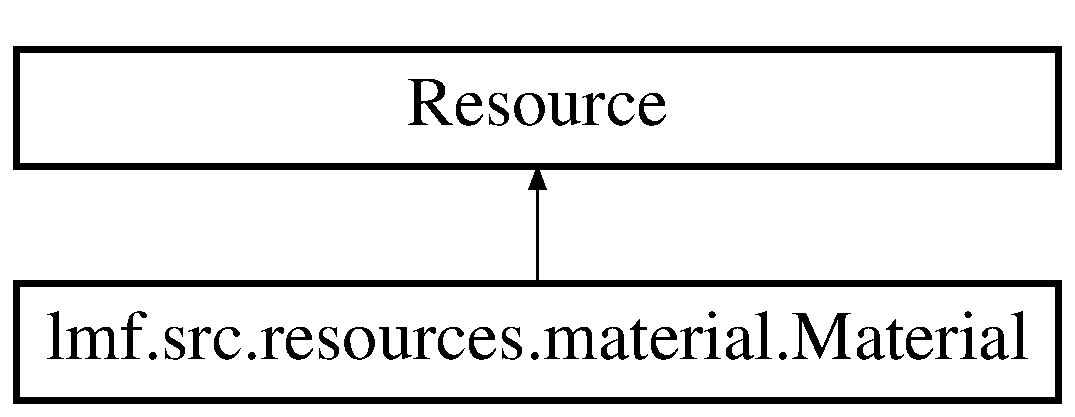
\includegraphics[height=2.000000cm]{classlmf_1_1src_1_1resources_1_1material_1_1_material}
\end{center}
\end{figure}
\subsection*{Public Member Functions}
\begin{DoxyCompactItemize}
\item 
def \hyperlink{classlmf_1_1src_1_1resources_1_1material_1_1_material_af93c831604873840e4b8f55949c28908}{\+\_\+\+\_\+init\+\_\+\+\_\+}
\begin{DoxyCompactList}\small\item\em As \hyperlink{classlmf_1_1src_1_1resources_1_1material_1_1_material}{Material} is an abstract class, constructor raises an error. \end{DoxyCompactList}\item 
def \hyperlink{classlmf_1_1src_1_1resources_1_1material_1_1_material_aeb5aef3dc67be13df017c088a396d94a}{\+\_\+\+\_\+del\+\_\+\+\_\+}
\begin{DoxyCompactList}\small\item\em As \hyperlink{classlmf_1_1src_1_1resources_1_1material_1_1_material}{Material} is an abstract class, desctructor raises an error. \end{DoxyCompactList}\item 
def \hyperlink{classlmf_1_1src_1_1resources_1_1material_1_1_material_a62fe17d9d1ceaf5efd1c2536f3957b32}{\+\_\+\+\_\+new\+\_\+\+\_\+}
\begin{DoxyCompactList}\small\item\em Private initialization called from \hyperlink{classlmf_1_1src_1_1resources_1_1material_1_1_material}{Material} subclasses. \end{DoxyCompactList}\end{DoxyCompactItemize}
\subsection*{Public Attributes}
\begin{DoxyCompactItemize}
\item 
\hyperlink{classlmf_1_1src_1_1resources_1_1material_1_1_material_ab41c0ac48aa33b79087a6fa568836a4a}{media\+Type}
\item 
\hyperlink{classlmf_1_1src_1_1resources_1_1material_1_1_material_a51df3bf6cd710ff574713abde19b8752}{file\+Name}
\item 
\hyperlink{classlmf_1_1src_1_1resources_1_1material_1_1_material_aef7b8711bf9663d23434fab0332d0824}{author}
\end{DoxyCompactItemize}


\subsection{Detailed Description}
\hyperlink{classlmf_1_1src_1_1resources_1_1material_1_1_material}{Material} is a Resource subclass. 

\hyperlink{classlmf_1_1src_1_1resources_1_1material_1_1_material}{Material} is an abstract class representing an audiovisual resource\+: an audio recording, a picture or a video. The \hyperlink{classlmf_1_1src_1_1resources_1_1material_1_1_material}{Material} class allows subclasses. 

Definition at line 8 of file material.\+py.



\subsection{Constructor \& Destructor Documentation}
\hypertarget{classlmf_1_1src_1_1resources_1_1material_1_1_material_af93c831604873840e4b8f55949c28908}{\index{lmf\+::src\+::resources\+::material\+::\+Material@{lmf\+::src\+::resources\+::material\+::\+Material}!\+\_\+\+\_\+init\+\_\+\+\_\+@{\+\_\+\+\_\+init\+\_\+\+\_\+}}
\index{\+\_\+\+\_\+init\+\_\+\+\_\+@{\+\_\+\+\_\+init\+\_\+\+\_\+}!lmf\+::src\+::resources\+::material\+::\+Material@{lmf\+::src\+::resources\+::material\+::\+Material}}
\subsubsection[{\+\_\+\+\_\+init\+\_\+\+\_\+}]{\setlength{\rightskip}{0pt plus 5cm}def lmf.\+src.\+resources.\+material.\+Material.\+\_\+\+\_\+init\+\_\+\+\_\+ (
\begin{DoxyParamCaption}
\item[{}]{self}
\end{DoxyParamCaption}
)}}\label{classlmf_1_1src_1_1resources_1_1material_1_1_material_af93c831604873840e4b8f55949c28908}


As \hyperlink{classlmf_1_1src_1_1resources_1_1material_1_1_material}{Material} is an abstract class, constructor raises an error. 



Definition at line 11 of file material.\+py.

\hypertarget{classlmf_1_1src_1_1resources_1_1material_1_1_material_aeb5aef3dc67be13df017c088a396d94a}{\index{lmf\+::src\+::resources\+::material\+::\+Material@{lmf\+::src\+::resources\+::material\+::\+Material}!\+\_\+\+\_\+del\+\_\+\+\_\+@{\+\_\+\+\_\+del\+\_\+\+\_\+}}
\index{\+\_\+\+\_\+del\+\_\+\+\_\+@{\+\_\+\+\_\+del\+\_\+\+\_\+}!lmf\+::src\+::resources\+::material\+::\+Material@{lmf\+::src\+::resources\+::material\+::\+Material}}
\subsubsection[{\+\_\+\+\_\+del\+\_\+\+\_\+}]{\setlength{\rightskip}{0pt plus 5cm}def lmf.\+src.\+resources.\+material.\+Material.\+\_\+\+\_\+del\+\_\+\+\_\+ (
\begin{DoxyParamCaption}
\item[{}]{self}
\end{DoxyParamCaption}
)}}\label{classlmf_1_1src_1_1resources_1_1material_1_1_material_aeb5aef3dc67be13df017c088a396d94a}


As \hyperlink{classlmf_1_1src_1_1resources_1_1material_1_1_material}{Material} is an abstract class, desctructor raises an error. 



Definition at line 16 of file material.\+py.



\subsection{Member Function Documentation}
\hypertarget{classlmf_1_1src_1_1resources_1_1material_1_1_material_a62fe17d9d1ceaf5efd1c2536f3957b32}{\index{lmf\+::src\+::resources\+::material\+::\+Material@{lmf\+::src\+::resources\+::material\+::\+Material}!\+\_\+\+\_\+new\+\_\+\+\_\+@{\+\_\+\+\_\+new\+\_\+\+\_\+}}
\index{\+\_\+\+\_\+new\+\_\+\+\_\+@{\+\_\+\+\_\+new\+\_\+\+\_\+}!lmf\+::src\+::resources\+::material\+::\+Material@{lmf\+::src\+::resources\+::material\+::\+Material}}
\subsubsection[{\+\_\+\+\_\+new\+\_\+\+\_\+}]{\setlength{\rightskip}{0pt plus 5cm}def lmf.\+src.\+resources.\+material.\+Material.\+\_\+\+\_\+new\+\_\+\+\_\+ (
\begin{DoxyParamCaption}
\item[{}]{self}
\end{DoxyParamCaption}
)}}\label{classlmf_1_1src_1_1resources_1_1material_1_1_material_a62fe17d9d1ceaf5efd1c2536f3957b32}


Private initialization called from \hyperlink{classlmf_1_1src_1_1resources_1_1material_1_1_material}{Material} subclasses. 

\hyperlink{classlmf_1_1src_1_1resources_1_1material_1_1_material}{Material} subinstances are owned by Form\+Representation. 

Definition at line 21 of file material.\+py.



\subsection{Member Data Documentation}
\hypertarget{classlmf_1_1src_1_1resources_1_1material_1_1_material_aef7b8711bf9663d23434fab0332d0824}{\index{lmf\+::src\+::resources\+::material\+::\+Material@{lmf\+::src\+::resources\+::material\+::\+Material}!author@{author}}
\index{author@{author}!lmf\+::src\+::resources\+::material\+::\+Material@{lmf\+::src\+::resources\+::material\+::\+Material}}
\subsubsection[{author}]{\setlength{\rightskip}{0pt plus 5cm}lmf.\+src.\+resources.\+material.\+Material.\+author}}\label{classlmf_1_1src_1_1resources_1_1material_1_1_material_aef7b8711bf9663d23434fab0332d0824}


Definition at line 27 of file material.\+py.

\hypertarget{classlmf_1_1src_1_1resources_1_1material_1_1_material_a51df3bf6cd710ff574713abde19b8752}{\index{lmf\+::src\+::resources\+::material\+::\+Material@{lmf\+::src\+::resources\+::material\+::\+Material}!file\+Name@{file\+Name}}
\index{file\+Name@{file\+Name}!lmf\+::src\+::resources\+::material\+::\+Material@{lmf\+::src\+::resources\+::material\+::\+Material}}
\subsubsection[{file\+Name}]{\setlength{\rightskip}{0pt plus 5cm}lmf.\+src.\+resources.\+material.\+Material.\+file\+Name}}\label{classlmf_1_1src_1_1resources_1_1material_1_1_material_a51df3bf6cd710ff574713abde19b8752}


Definition at line 26 of file material.\+py.

\hypertarget{classlmf_1_1src_1_1resources_1_1material_1_1_material_ab41c0ac48aa33b79087a6fa568836a4a}{\index{lmf\+::src\+::resources\+::material\+::\+Material@{lmf\+::src\+::resources\+::material\+::\+Material}!media\+Type@{media\+Type}}
\index{media\+Type@{media\+Type}!lmf\+::src\+::resources\+::material\+::\+Material@{lmf\+::src\+::resources\+::material\+::\+Material}}
\subsubsection[{media\+Type}]{\setlength{\rightskip}{0pt plus 5cm}lmf.\+src.\+resources.\+material.\+Material.\+media\+Type}}\label{classlmf_1_1src_1_1resources_1_1material_1_1_material_ab41c0ac48aa33b79087a6fa568836a4a}


Definition at line 25 of file material.\+py.



The documentation for this class was generated from the following file\+:\begin{DoxyCompactItemize}
\item 
/\+Users/celine/\+Work/\+C\+N\+R\+S/workspace/\+Himal\+Co/dev/lib/lmf/src/resources/\hyperlink{material_8py}{material.\+py}\end{DoxyCompactItemize}

\hypertarget{classlmf_1_1src_1_1utils_1_1error__handling_1_1_output_error}{\section{lmf.\+src.\+utils.\+error\+\_\+handling.\+Output\+Error Class Reference}
\label{classlmf_1_1src_1_1utils_1_1error__handling_1_1_output_error}\index{lmf.\+src.\+utils.\+error\+\_\+handling.\+Output\+Error@{lmf.\+src.\+utils.\+error\+\_\+handling.\+Output\+Error}}
}


Exception raised for errors in the output.  


Inheritance diagram for lmf.\+src.\+utils.\+error\+\_\+handling.\+Output\+Error\+:\begin{figure}[H]
\begin{center}
\leavevmode
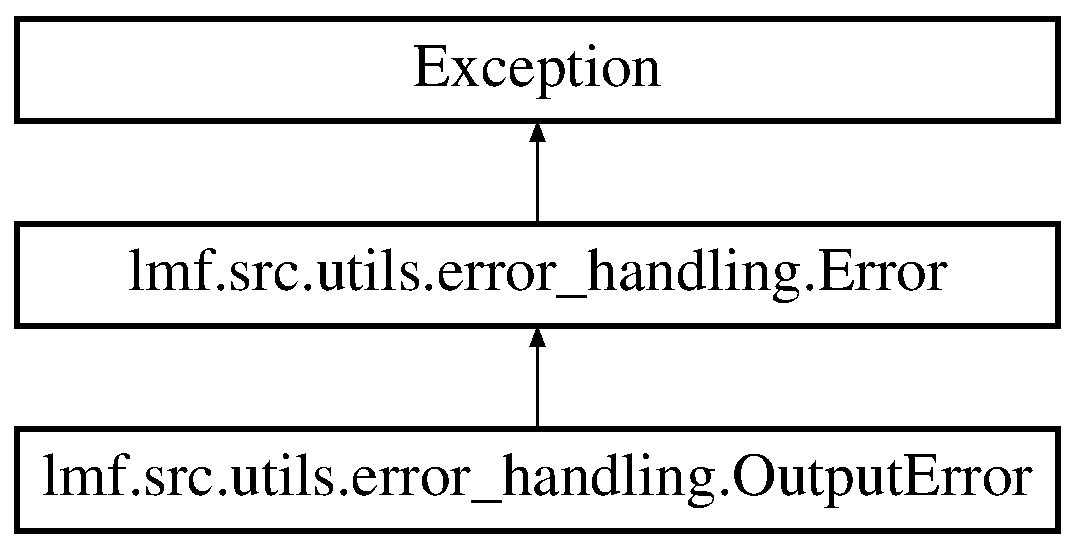
\includegraphics[height=3.000000cm]{classlmf_1_1src_1_1utils_1_1error__handling_1_1_output_error}
\end{center}
\end{figure}
\subsection*{Public Member Functions}
\begin{DoxyCompactItemize}
\item 
def \hyperlink{classlmf_1_1src_1_1utils_1_1error__handling_1_1_output_error_ae8b17e571a6cda3419da8e5d157817ac}{\+\_\+\+\_\+init\+\_\+\+\_\+}
\begin{DoxyCompactList}\small\item\em Constructor. \end{DoxyCompactList}\item 
def \hyperlink{classlmf_1_1src_1_1utils_1_1error__handling_1_1_output_error_adacfd84a3c64b1606a39f744f031e1a6}{handle}
\begin{DoxyCompactList}\small\item\em Define behavior to follow in case this error is caught\+: display error and exit program. \end{DoxyCompactList}\end{DoxyCompactItemize}
\subsection*{Public Attributes}
\begin{DoxyCompactItemize}
\item 
\hyperlink{classlmf_1_1src_1_1utils_1_1error__handling_1_1_output_error_a4bdad4fe4219a12ae88039ee8633c316}{msg}
\item 
\hyperlink{classlmf_1_1src_1_1utils_1_1error__handling_1_1_output_error_a0b89f6a37fac3415e278b996f2ba8117}{expr}
\item 
\hyperlink{classlmf_1_1src_1_1utils_1_1error__handling_1_1_output_error_aa9cde9b3f989c8465f12e1b6e3b715bb}{frame\+\_\+info}
\end{DoxyCompactItemize}


\subsection{Detailed Description}
Exception raised for errors in the output. 

Definition at line 69 of file error\+\_\+handling.\+py.



\subsection{Constructor \& Destructor Documentation}
\hypertarget{classlmf_1_1src_1_1utils_1_1error__handling_1_1_output_error_ae8b17e571a6cda3419da8e5d157817ac}{\index{lmf\+::src\+::utils\+::error\+\_\+handling\+::\+Output\+Error@{lmf\+::src\+::utils\+::error\+\_\+handling\+::\+Output\+Error}!\+\_\+\+\_\+init\+\_\+\+\_\+@{\+\_\+\+\_\+init\+\_\+\+\_\+}}
\index{\+\_\+\+\_\+init\+\_\+\+\_\+@{\+\_\+\+\_\+init\+\_\+\+\_\+}!lmf\+::src\+::utils\+::error\+\_\+handling\+::\+Output\+Error@{lmf\+::src\+::utils\+::error\+\_\+handling\+::\+Output\+Error}}
\subsubsection[{\+\_\+\+\_\+init\+\_\+\+\_\+}]{\setlength{\rightskip}{0pt plus 5cm}def lmf.\+src.\+utils.\+error\+\_\+handling.\+Output\+Error.\+\_\+\+\_\+init\+\_\+\+\_\+ (
\begin{DoxyParamCaption}
\item[{}]{self, }
\item[{}]{msg, }
\item[{}]{expr = {\ttfamily None}}
\end{DoxyParamCaption}
)}}\label{classlmf_1_1src_1_1utils_1_1error__handling_1_1_output_error_ae8b17e571a6cda3419da8e5d157817ac}


Constructor. 


\begin{DoxyParams}{Parameters}
{\em msg} & Explanation of the error. \\
\hline
{\em expr} & Output expression in which the error occurred. \\
\hline
\end{DoxyParams}
\begin{DoxyReturn}{Returns}
An \hyperlink{classlmf_1_1src_1_1utils_1_1error__handling_1_1_output_error}{Output\+Error} instance. 
\end{DoxyReturn}


Definition at line 72 of file error\+\_\+handling.\+py.



\subsection{Member Function Documentation}
\hypertarget{classlmf_1_1src_1_1utils_1_1error__handling_1_1_output_error_adacfd84a3c64b1606a39f744f031e1a6}{\index{lmf\+::src\+::utils\+::error\+\_\+handling\+::\+Output\+Error@{lmf\+::src\+::utils\+::error\+\_\+handling\+::\+Output\+Error}!handle@{handle}}
\index{handle@{handle}!lmf\+::src\+::utils\+::error\+\_\+handling\+::\+Output\+Error@{lmf\+::src\+::utils\+::error\+\_\+handling\+::\+Output\+Error}}
\subsubsection[{handle}]{\setlength{\rightskip}{0pt plus 5cm}def lmf.\+src.\+utils.\+error\+\_\+handling.\+Output\+Error.\+handle (
\begin{DoxyParamCaption}
\item[{}]{self}
\end{DoxyParamCaption}
)}}\label{classlmf_1_1src_1_1utils_1_1error__handling_1_1_output_error_adacfd84a3c64b1606a39f744f031e1a6}


Define behavior to follow in case this error is caught\+: display error and exit program. 



Definition at line 84 of file error\+\_\+handling.\+py.



\subsection{Member Data Documentation}
\hypertarget{classlmf_1_1src_1_1utils_1_1error__handling_1_1_output_error_a0b89f6a37fac3415e278b996f2ba8117}{\index{lmf\+::src\+::utils\+::error\+\_\+handling\+::\+Output\+Error@{lmf\+::src\+::utils\+::error\+\_\+handling\+::\+Output\+Error}!expr@{expr}}
\index{expr@{expr}!lmf\+::src\+::utils\+::error\+\_\+handling\+::\+Output\+Error@{lmf\+::src\+::utils\+::error\+\_\+handling\+::\+Output\+Error}}
\subsubsection[{expr}]{\setlength{\rightskip}{0pt plus 5cm}lmf.\+src.\+utils.\+error\+\_\+handling.\+Output\+Error.\+expr}}\label{classlmf_1_1src_1_1utils_1_1error__handling_1_1_output_error_a0b89f6a37fac3415e278b996f2ba8117}


Definition at line 79 of file error\+\_\+handling.\+py.

\hypertarget{classlmf_1_1src_1_1utils_1_1error__handling_1_1_output_error_aa9cde9b3f989c8465f12e1b6e3b715bb}{\index{lmf\+::src\+::utils\+::error\+\_\+handling\+::\+Output\+Error@{lmf\+::src\+::utils\+::error\+\_\+handling\+::\+Output\+Error}!frame\+\_\+info@{frame\+\_\+info}}
\index{frame\+\_\+info@{frame\+\_\+info}!lmf\+::src\+::utils\+::error\+\_\+handling\+::\+Output\+Error@{lmf\+::src\+::utils\+::error\+\_\+handling\+::\+Output\+Error}}
\subsubsection[{frame\+\_\+info}]{\setlength{\rightskip}{0pt plus 5cm}lmf.\+src.\+utils.\+error\+\_\+handling.\+Output\+Error.\+frame\+\_\+info}}\label{classlmf_1_1src_1_1utils_1_1error__handling_1_1_output_error_aa9cde9b3f989c8465f12e1b6e3b715bb}


Definition at line 82 of file error\+\_\+handling.\+py.

\hypertarget{classlmf_1_1src_1_1utils_1_1error__handling_1_1_output_error_a4bdad4fe4219a12ae88039ee8633c316}{\index{lmf\+::src\+::utils\+::error\+\_\+handling\+::\+Output\+Error@{lmf\+::src\+::utils\+::error\+\_\+handling\+::\+Output\+Error}!msg@{msg}}
\index{msg@{msg}!lmf\+::src\+::utils\+::error\+\_\+handling\+::\+Output\+Error@{lmf\+::src\+::utils\+::error\+\_\+handling\+::\+Output\+Error}}
\subsubsection[{msg}]{\setlength{\rightskip}{0pt plus 5cm}lmf.\+src.\+utils.\+error\+\_\+handling.\+Output\+Error.\+msg}}\label{classlmf_1_1src_1_1utils_1_1error__handling_1_1_output_error_a4bdad4fe4219a12ae88039ee8633c316}


Definition at line 78 of file error\+\_\+handling.\+py.



The documentation for this class was generated from the following file\+:\begin{DoxyCompactItemize}
\item 
/\+Users/celine/\+Work/\+C\+N\+R\+S/workspace/\+Himal\+Co/dev/lib/lmf/src/utils/\hyperlink{error__handling_8py}{error\+\_\+handling.\+py}\end{DoxyCompactItemize}

\hypertarget{classlmf_1_1src_1_1morphosyntax_1_1paradigm_1_1_paradigm}{\section{lmf.\+src.\+morphosyntax.\+paradigm.\+Paradigm Class Reference}
\label{classlmf_1_1src_1_1morphosyntax_1_1paradigm_1_1_paradigm}\index{lmf.\+src.\+morphosyntax.\+paradigm.\+Paradigm@{lmf.\+src.\+morphosyntax.\+paradigm.\+Paradigm}}
}


\hyperlink{classlmf_1_1src_1_1morphosyntax_1_1paradigm_1_1_paradigm}{Paradigm} is a class representing a morphological paradigm.  


\subsection*{Public Member Functions}
\begin{DoxyCompactItemize}
\item 
def \hyperlink{classlmf_1_1src_1_1morphosyntax_1_1paradigm_1_1_paradigm_ab0c529b6dfdc802436aaee80cc7a3f1a}{\+\_\+\+\_\+init\+\_\+\+\_\+}
\begin{DoxyCompactList}\small\item\em Constructor. \end{DoxyCompactList}\item 
def \hyperlink{classlmf_1_1src_1_1morphosyntax_1_1paradigm_1_1_paradigm_a27ffcc1bdb76712e7d8b31de78412f8a}{\+\_\+\+\_\+del\+\_\+\+\_\+}
\begin{DoxyCompactList}\small\item\em Destructor. \end{DoxyCompactList}\item 
def \hyperlink{classlmf_1_1src_1_1morphosyntax_1_1paradigm_1_1_paradigm_abe500cbb370628c4945b6433124f0f05}{set\+\_\+paradigm\+Label}
\begin{DoxyCompactList}\small\item\em Set paradigm label. \end{DoxyCompactList}\item 
def \hyperlink{classlmf_1_1src_1_1morphosyntax_1_1paradigm_1_1_paradigm_ab90570fe38c57469e05359af8806c017}{get\+\_\+paradigm\+Label}
\begin{DoxyCompactList}\small\item\em Get paradigm label. \end{DoxyCompactList}\item 
def \hyperlink{classlmf_1_1src_1_1morphosyntax_1_1paradigm_1_1_paradigm_a31c24b8f0fdbf375a4a64f8c37a74825}{set\+\_\+paradigm}
\begin{DoxyCompactList}\small\item\em Set paradigm. \end{DoxyCompactList}\item 
def \hyperlink{classlmf_1_1src_1_1morphosyntax_1_1paradigm_1_1_paradigm_afe61d3e21fd13270af987b702304b449}{get\+\_\+paradigm}
\begin{DoxyCompactList}\small\item\em Get paradigm. \end{DoxyCompactList}\item 
def \hyperlink{classlmf_1_1src_1_1morphosyntax_1_1paradigm_1_1_paradigm_a142b0411391ae7842710e1e086420a40}{set\+\_\+language}
\begin{DoxyCompactList}\small\item\em Set language of the paradigm. \end{DoxyCompactList}\item 
def \hyperlink{classlmf_1_1src_1_1morphosyntax_1_1paradigm_1_1_paradigm_a7ba7ef75fdd20edfddc8821c7d4eca9a}{get\+\_\+language}
\begin{DoxyCompactList}\small\item\em Get paradigm language. \end{DoxyCompactList}\item 
def \hyperlink{classlmf_1_1src_1_1morphosyntax_1_1paradigm_1_1_paradigm_a40a98ba766025f62f839299c4084666c}{set\+\_\+morphology}
\begin{DoxyCompactList}\small\item\em Set morphology. \end{DoxyCompactList}\item 
def \hyperlink{classlmf_1_1src_1_1morphosyntax_1_1paradigm_1_1_paradigm_a7f8b86d83993a56e5dd46a7924f130b4}{get\+\_\+morphology}
\begin{DoxyCompactList}\small\item\em Get morphology. \end{DoxyCompactList}\item 
def \hyperlink{classlmf_1_1src_1_1morphosyntax_1_1paradigm_1_1_paradigm_aa9cc39604cd3b3d06e1d142016db3541}{get\+\_\+lexical\+\_\+entry}
\begin{DoxyCompactList}\small\item\em Get pointed lexical entry. \end{DoxyCompactList}\end{DoxyCompactItemize}
\subsection*{Public Attributes}
\begin{DoxyCompactItemize}
\item 
\hyperlink{classlmf_1_1src_1_1morphosyntax_1_1paradigm_1_1_paradigm_a5892a515d2311d4c03b180603a0d2929}{paradigm\+Label}
\item 
\hyperlink{classlmf_1_1src_1_1morphosyntax_1_1paradigm_1_1_paradigm_a2c706c0653324f536c9fc8b20d5dbf15}{paradigm}
\item 
\hyperlink{classlmf_1_1src_1_1morphosyntax_1_1paradigm_1_1_paradigm_a536c9155740d0363044389ce31dff090}{language}
\item 
\hyperlink{classlmf_1_1src_1_1morphosyntax_1_1paradigm_1_1_paradigm_a7c9c944b764a0351f0e58234b48bdf86}{morphology}
\item 
\hyperlink{classlmf_1_1src_1_1morphosyntax_1_1paradigm_1_1_paradigm_a546af1d9fc21b3b1a6d102e39877a587}{targets}
\end{DoxyCompactItemize}


\subsection{Detailed Description}
\hyperlink{classlmf_1_1src_1_1morphosyntax_1_1paradigm_1_1_paradigm}{Paradigm} is a class representing a morphological paradigm. 

Definition at line 10 of file paradigm.\+py.



\subsection{Constructor \& Destructor Documentation}
\hypertarget{classlmf_1_1src_1_1morphosyntax_1_1paradigm_1_1_paradigm_ab0c529b6dfdc802436aaee80cc7a3f1a}{\index{lmf\+::src\+::morphosyntax\+::paradigm\+::\+Paradigm@{lmf\+::src\+::morphosyntax\+::paradigm\+::\+Paradigm}!\+\_\+\+\_\+init\+\_\+\+\_\+@{\+\_\+\+\_\+init\+\_\+\+\_\+}}
\index{\+\_\+\+\_\+init\+\_\+\+\_\+@{\+\_\+\+\_\+init\+\_\+\+\_\+}!lmf\+::src\+::morphosyntax\+::paradigm\+::\+Paradigm@{lmf\+::src\+::morphosyntax\+::paradigm\+::\+Paradigm}}
\subsubsection[{\+\_\+\+\_\+init\+\_\+\+\_\+}]{\setlength{\rightskip}{0pt plus 5cm}def lmf.\+src.\+morphosyntax.\+paradigm.\+Paradigm.\+\_\+\+\_\+init\+\_\+\+\_\+ (
\begin{DoxyParamCaption}
\item[{}]{self}
\end{DoxyParamCaption}
)}}\label{classlmf_1_1src_1_1morphosyntax_1_1paradigm_1_1_paradigm_ab0c529b6dfdc802436aaee80cc7a3f1a}


Constructor. 

\hyperlink{classlmf_1_1src_1_1morphosyntax_1_1paradigm_1_1_paradigm}{Paradigm} instances are owned by Sense. \begin{DoxyReturn}{Returns}
A \hyperlink{classlmf_1_1src_1_1morphosyntax_1_1paradigm_1_1_paradigm}{Paradigm} instance. 
\end{DoxyReturn}


Definition at line 13 of file paradigm.\+py.

\hypertarget{classlmf_1_1src_1_1morphosyntax_1_1paradigm_1_1_paradigm_a27ffcc1bdb76712e7d8b31de78412f8a}{\index{lmf\+::src\+::morphosyntax\+::paradigm\+::\+Paradigm@{lmf\+::src\+::morphosyntax\+::paradigm\+::\+Paradigm}!\+\_\+\+\_\+del\+\_\+\+\_\+@{\+\_\+\+\_\+del\+\_\+\+\_\+}}
\index{\+\_\+\+\_\+del\+\_\+\+\_\+@{\+\_\+\+\_\+del\+\_\+\+\_\+}!lmf\+::src\+::morphosyntax\+::paradigm\+::\+Paradigm@{lmf\+::src\+::morphosyntax\+::paradigm\+::\+Paradigm}}
\subsubsection[{\+\_\+\+\_\+del\+\_\+\+\_\+}]{\setlength{\rightskip}{0pt plus 5cm}def lmf.\+src.\+morphosyntax.\+paradigm.\+Paradigm.\+\_\+\+\_\+del\+\_\+\+\_\+ (
\begin{DoxyParamCaption}
\item[{}]{self}
\end{DoxyParamCaption}
)}}\label{classlmf_1_1src_1_1morphosyntax_1_1paradigm_1_1_paradigm_a27ffcc1bdb76712e7d8b31de78412f8a}


Destructor. 



Definition at line 28 of file paradigm.\+py.



\subsection{Member Function Documentation}
\hypertarget{classlmf_1_1src_1_1morphosyntax_1_1paradigm_1_1_paradigm_a7ba7ef75fdd20edfddc8821c7d4eca9a}{\index{lmf\+::src\+::morphosyntax\+::paradigm\+::\+Paradigm@{lmf\+::src\+::morphosyntax\+::paradigm\+::\+Paradigm}!get\+\_\+language@{get\+\_\+language}}
\index{get\+\_\+language@{get\+\_\+language}!lmf\+::src\+::morphosyntax\+::paradigm\+::\+Paradigm@{lmf\+::src\+::morphosyntax\+::paradigm\+::\+Paradigm}}
\subsubsection[{get\+\_\+language}]{\setlength{\rightskip}{0pt plus 5cm}def lmf.\+src.\+morphosyntax.\+paradigm.\+Paradigm.\+get\+\_\+language (
\begin{DoxyParamCaption}
\item[{}]{self}
\end{DoxyParamCaption}
)}}\label{classlmf_1_1src_1_1morphosyntax_1_1paradigm_1_1_paradigm_a7ba7ef75fdd20edfddc8821c7d4eca9a}


Get paradigm language. 

\begin{DoxyReturn}{Returns}
\hyperlink{classlmf_1_1src_1_1morphosyntax_1_1paradigm_1_1_paradigm}{Paradigm} attribute 'language'. 
\end{DoxyReturn}


Definition at line 77 of file paradigm.\+py.

\hypertarget{classlmf_1_1src_1_1morphosyntax_1_1paradigm_1_1_paradigm_aa9cc39604cd3b3d06e1d142016db3541}{\index{lmf\+::src\+::morphosyntax\+::paradigm\+::\+Paradigm@{lmf\+::src\+::morphosyntax\+::paradigm\+::\+Paradigm}!get\+\_\+lexical\+\_\+entry@{get\+\_\+lexical\+\_\+entry}}
\index{get\+\_\+lexical\+\_\+entry@{get\+\_\+lexical\+\_\+entry}!lmf\+::src\+::morphosyntax\+::paradigm\+::\+Paradigm@{lmf\+::src\+::morphosyntax\+::paradigm\+::\+Paradigm}}
\subsubsection[{get\+\_\+lexical\+\_\+entry}]{\setlength{\rightskip}{0pt plus 5cm}def lmf.\+src.\+morphosyntax.\+paradigm.\+Paradigm.\+get\+\_\+lexical\+\_\+entry (
\begin{DoxyParamCaption}
\item[{}]{self}
\end{DoxyParamCaption}
)}}\label{classlmf_1_1src_1_1morphosyntax_1_1paradigm_1_1_paradigm_aa9cc39604cd3b3d06e1d142016db3541}


Get pointed lexical entry. 

\begin{DoxyReturn}{Returns}
\hyperlink{classlmf_1_1src_1_1morphosyntax_1_1paradigm_1_1_paradigm}{Paradigm} private attribute '\+\_\+\+\_\+lexical\+\_\+entry'. 
\end{DoxyReturn}


Definition at line 97 of file paradigm.\+py.

\hypertarget{classlmf_1_1src_1_1morphosyntax_1_1paradigm_1_1_paradigm_a7f8b86d83993a56e5dd46a7924f130b4}{\index{lmf\+::src\+::morphosyntax\+::paradigm\+::\+Paradigm@{lmf\+::src\+::morphosyntax\+::paradigm\+::\+Paradigm}!get\+\_\+morphology@{get\+\_\+morphology}}
\index{get\+\_\+morphology@{get\+\_\+morphology}!lmf\+::src\+::morphosyntax\+::paradigm\+::\+Paradigm@{lmf\+::src\+::morphosyntax\+::paradigm\+::\+Paradigm}}
\subsubsection[{get\+\_\+morphology}]{\setlength{\rightskip}{0pt plus 5cm}def lmf.\+src.\+morphosyntax.\+paradigm.\+Paradigm.\+get\+\_\+morphology (
\begin{DoxyParamCaption}
\item[{}]{self}
\end{DoxyParamCaption}
)}}\label{classlmf_1_1src_1_1morphosyntax_1_1paradigm_1_1_paradigm_a7f8b86d83993a56e5dd46a7924f130b4}


Get morphology. 

\begin{DoxyReturn}{Returns}
\hyperlink{classlmf_1_1src_1_1morphosyntax_1_1paradigm_1_1_paradigm}{Paradigm} attribute 'morphology'. 
\end{DoxyReturn}


Definition at line 91 of file paradigm.\+py.

\hypertarget{classlmf_1_1src_1_1morphosyntax_1_1paradigm_1_1_paradigm_afe61d3e21fd13270af987b702304b449}{\index{lmf\+::src\+::morphosyntax\+::paradigm\+::\+Paradigm@{lmf\+::src\+::morphosyntax\+::paradigm\+::\+Paradigm}!get\+\_\+paradigm@{get\+\_\+paradigm}}
\index{get\+\_\+paradigm@{get\+\_\+paradigm}!lmf\+::src\+::morphosyntax\+::paradigm\+::\+Paradigm@{lmf\+::src\+::morphosyntax\+::paradigm\+::\+Paradigm}}
\subsubsection[{get\+\_\+paradigm}]{\setlength{\rightskip}{0pt plus 5cm}def lmf.\+src.\+morphosyntax.\+paradigm.\+Paradigm.\+get\+\_\+paradigm (
\begin{DoxyParamCaption}
\item[{}]{self, }
\item[{}]{language = {\ttfamily None}}
\end{DoxyParamCaption}
)}}\label{classlmf_1_1src_1_1morphosyntax_1_1paradigm_1_1_paradigm_afe61d3e21fd13270af987b702304b449}


Get paradigm. 


\begin{DoxyParams}{Parameters}
{\em language} & Language filter. \\
\hline
\end{DoxyParams}
\begin{DoxyReturn}{Returns}
\hyperlink{classlmf_1_1src_1_1morphosyntax_1_1paradigm_1_1_paradigm}{Paradigm} attribute 'paradigm'. 
\end{DoxyReturn}


Definition at line 59 of file paradigm.\+py.

\hypertarget{classlmf_1_1src_1_1morphosyntax_1_1paradigm_1_1_paradigm_ab90570fe38c57469e05359af8806c017}{\index{lmf\+::src\+::morphosyntax\+::paradigm\+::\+Paradigm@{lmf\+::src\+::morphosyntax\+::paradigm\+::\+Paradigm}!get\+\_\+paradigm\+Label@{get\+\_\+paradigm\+Label}}
\index{get\+\_\+paradigm\+Label@{get\+\_\+paradigm\+Label}!lmf\+::src\+::morphosyntax\+::paradigm\+::\+Paradigm@{lmf\+::src\+::morphosyntax\+::paradigm\+::\+Paradigm}}
\subsubsection[{get\+\_\+paradigm\+Label}]{\setlength{\rightskip}{0pt plus 5cm}def lmf.\+src.\+morphosyntax.\+paradigm.\+Paradigm.\+get\+\_\+paradigm\+Label (
\begin{DoxyParamCaption}
\item[{}]{self}
\end{DoxyParamCaption}
)}}\label{classlmf_1_1src_1_1morphosyntax_1_1paradigm_1_1_paradigm_ab90570fe38c57469e05359af8806c017}


Get paradigm label. 

\begin{DoxyReturn}{Returns}
\hyperlink{classlmf_1_1src_1_1morphosyntax_1_1paradigm_1_1_paradigm}{Paradigm} attribute 'paradigm\+Label'. 
\end{DoxyReturn}


Definition at line 45 of file paradigm.\+py.

\hypertarget{classlmf_1_1src_1_1morphosyntax_1_1paradigm_1_1_paradigm_a142b0411391ae7842710e1e086420a40}{\index{lmf\+::src\+::morphosyntax\+::paradigm\+::\+Paradigm@{lmf\+::src\+::morphosyntax\+::paradigm\+::\+Paradigm}!set\+\_\+language@{set\+\_\+language}}
\index{set\+\_\+language@{set\+\_\+language}!lmf\+::src\+::morphosyntax\+::paradigm\+::\+Paradigm@{lmf\+::src\+::morphosyntax\+::paradigm\+::\+Paradigm}}
\subsubsection[{set\+\_\+language}]{\setlength{\rightskip}{0pt plus 5cm}def lmf.\+src.\+morphosyntax.\+paradigm.\+Paradigm.\+set\+\_\+language (
\begin{DoxyParamCaption}
\item[{}]{self, }
\item[{}]{language}
\end{DoxyParamCaption}
)}}\label{classlmf_1_1src_1_1morphosyntax_1_1paradigm_1_1_paradigm_a142b0411391ae7842710e1e086420a40}


Set language of the paradigm. 


\begin{DoxyParams}{Parameters}
{\em language} & The paradigm language to set. \\
\hline
\end{DoxyParams}
\begin{DoxyReturn}{Returns}
\hyperlink{classlmf_1_1src_1_1morphosyntax_1_1paradigm_1_1_paradigm}{Paradigm} instance. 
\end{DoxyReturn}


Definition at line 69 of file paradigm.\+py.

\hypertarget{classlmf_1_1src_1_1morphosyntax_1_1paradigm_1_1_paradigm_a40a98ba766025f62f839299c4084666c}{\index{lmf\+::src\+::morphosyntax\+::paradigm\+::\+Paradigm@{lmf\+::src\+::morphosyntax\+::paradigm\+::\+Paradigm}!set\+\_\+morphology@{set\+\_\+morphology}}
\index{set\+\_\+morphology@{set\+\_\+morphology}!lmf\+::src\+::morphosyntax\+::paradigm\+::\+Paradigm@{lmf\+::src\+::morphosyntax\+::paradigm\+::\+Paradigm}}
\subsubsection[{set\+\_\+morphology}]{\setlength{\rightskip}{0pt plus 5cm}def lmf.\+src.\+morphosyntax.\+paradigm.\+Paradigm.\+set\+\_\+morphology (
\begin{DoxyParamCaption}
\item[{}]{self, }
\item[{}]{morphology}
\end{DoxyParamCaption}
)}}\label{classlmf_1_1src_1_1morphosyntax_1_1paradigm_1_1_paradigm_a40a98ba766025f62f839299c4084666c}


Set morphology. 


\begin{DoxyParams}{Parameters}
{\em morphology} & The morphology to set. \\
\hline
\end{DoxyParams}
\begin{DoxyReturn}{Returns}
\hyperlink{classlmf_1_1src_1_1morphosyntax_1_1paradigm_1_1_paradigm}{Paradigm} instance. 
\end{DoxyReturn}


Definition at line 83 of file paradigm.\+py.

\hypertarget{classlmf_1_1src_1_1morphosyntax_1_1paradigm_1_1_paradigm_a31c24b8f0fdbf375a4a64f8c37a74825}{\index{lmf\+::src\+::morphosyntax\+::paradigm\+::\+Paradigm@{lmf\+::src\+::morphosyntax\+::paradigm\+::\+Paradigm}!set\+\_\+paradigm@{set\+\_\+paradigm}}
\index{set\+\_\+paradigm@{set\+\_\+paradigm}!lmf\+::src\+::morphosyntax\+::paradigm\+::\+Paradigm@{lmf\+::src\+::morphosyntax\+::paradigm\+::\+Paradigm}}
\subsubsection[{set\+\_\+paradigm}]{\setlength{\rightskip}{0pt plus 5cm}def lmf.\+src.\+morphosyntax.\+paradigm.\+Paradigm.\+set\+\_\+paradigm (
\begin{DoxyParamCaption}
\item[{}]{self, }
\item[{}]{paradigm}
\end{DoxyParamCaption}
)}}\label{classlmf_1_1src_1_1morphosyntax_1_1paradigm_1_1_paradigm_a31c24b8f0fdbf375a4a64f8c37a74825}


Set paradigm. 


\begin{DoxyParams}{Parameters}
{\em paradigm} & The paradigm to set. \\
\hline
\end{DoxyParams}
\begin{DoxyReturn}{Returns}
\hyperlink{classlmf_1_1src_1_1morphosyntax_1_1paradigm_1_1_paradigm}{Paradigm} instance. 
\end{DoxyReturn}


Definition at line 51 of file paradigm.\+py.

\hypertarget{classlmf_1_1src_1_1morphosyntax_1_1paradigm_1_1_paradigm_abe500cbb370628c4945b6433124f0f05}{\index{lmf\+::src\+::morphosyntax\+::paradigm\+::\+Paradigm@{lmf\+::src\+::morphosyntax\+::paradigm\+::\+Paradigm}!set\+\_\+paradigm\+Label@{set\+\_\+paradigm\+Label}}
\index{set\+\_\+paradigm\+Label@{set\+\_\+paradigm\+Label}!lmf\+::src\+::morphosyntax\+::paradigm\+::\+Paradigm@{lmf\+::src\+::morphosyntax\+::paradigm\+::\+Paradigm}}
\subsubsection[{set\+\_\+paradigm\+Label}]{\setlength{\rightskip}{0pt plus 5cm}def lmf.\+src.\+morphosyntax.\+paradigm.\+Paradigm.\+set\+\_\+paradigm\+Label (
\begin{DoxyParamCaption}
\item[{}]{self, }
\item[{}]{paradigm\+\_\+label}
\end{DoxyParamCaption}
)}}\label{classlmf_1_1src_1_1morphosyntax_1_1paradigm_1_1_paradigm_abe500cbb370628c4945b6433124f0f05}


Set paradigm label. 


\begin{DoxyParams}{Parameters}
{\em paradigm\+\_\+label} & The paradigm label to set. \\
\hline
\end{DoxyParams}
\begin{DoxyReturn}{Returns}
\hyperlink{classlmf_1_1src_1_1morphosyntax_1_1paradigm_1_1_paradigm}{Paradigm} instance. 
\end{DoxyReturn}


Definition at line 34 of file paradigm.\+py.



\subsection{Member Data Documentation}
\hypertarget{classlmf_1_1src_1_1morphosyntax_1_1paradigm_1_1_paradigm_a536c9155740d0363044389ce31dff090}{\index{lmf\+::src\+::morphosyntax\+::paradigm\+::\+Paradigm@{lmf\+::src\+::morphosyntax\+::paradigm\+::\+Paradigm}!language@{language}}
\index{language@{language}!lmf\+::src\+::morphosyntax\+::paradigm\+::\+Paradigm@{lmf\+::src\+::morphosyntax\+::paradigm\+::\+Paradigm}}
\subsubsection[{language}]{\setlength{\rightskip}{0pt plus 5cm}lmf.\+src.\+morphosyntax.\+paradigm.\+Paradigm.\+language}}\label{classlmf_1_1src_1_1morphosyntax_1_1paradigm_1_1_paradigm_a536c9155740d0363044389ce31dff090}


Definition at line 20 of file paradigm.\+py.

\hypertarget{classlmf_1_1src_1_1morphosyntax_1_1paradigm_1_1_paradigm_a7c9c944b764a0351f0e58234b48bdf86}{\index{lmf\+::src\+::morphosyntax\+::paradigm\+::\+Paradigm@{lmf\+::src\+::morphosyntax\+::paradigm\+::\+Paradigm}!morphology@{morphology}}
\index{morphology@{morphology}!lmf\+::src\+::morphosyntax\+::paradigm\+::\+Paradigm@{lmf\+::src\+::morphosyntax\+::paradigm\+::\+Paradigm}}
\subsubsection[{morphology}]{\setlength{\rightskip}{0pt plus 5cm}lmf.\+src.\+morphosyntax.\+paradigm.\+Paradigm.\+morphology}}\label{classlmf_1_1src_1_1morphosyntax_1_1paradigm_1_1_paradigm_a7c9c944b764a0351f0e58234b48bdf86}


Definition at line 21 of file paradigm.\+py.

\hypertarget{classlmf_1_1src_1_1morphosyntax_1_1paradigm_1_1_paradigm_a2c706c0653324f536c9fc8b20d5dbf15}{\index{lmf\+::src\+::morphosyntax\+::paradigm\+::\+Paradigm@{lmf\+::src\+::morphosyntax\+::paradigm\+::\+Paradigm}!paradigm@{paradigm}}
\index{paradigm@{paradigm}!lmf\+::src\+::morphosyntax\+::paradigm\+::\+Paradigm@{lmf\+::src\+::morphosyntax\+::paradigm\+::\+Paradigm}}
\subsubsection[{paradigm}]{\setlength{\rightskip}{0pt plus 5cm}lmf.\+src.\+morphosyntax.\+paradigm.\+Paradigm.\+paradigm}}\label{classlmf_1_1src_1_1morphosyntax_1_1paradigm_1_1_paradigm_a2c706c0653324f536c9fc8b20d5dbf15}


Definition at line 19 of file paradigm.\+py.

\hypertarget{classlmf_1_1src_1_1morphosyntax_1_1paradigm_1_1_paradigm_a5892a515d2311d4c03b180603a0d2929}{\index{lmf\+::src\+::morphosyntax\+::paradigm\+::\+Paradigm@{lmf\+::src\+::morphosyntax\+::paradigm\+::\+Paradigm}!paradigm\+Label@{paradigm\+Label}}
\index{paradigm\+Label@{paradigm\+Label}!lmf\+::src\+::morphosyntax\+::paradigm\+::\+Paradigm@{lmf\+::src\+::morphosyntax\+::paradigm\+::\+Paradigm}}
\subsubsection[{paradigm\+Label}]{\setlength{\rightskip}{0pt plus 5cm}lmf.\+src.\+morphosyntax.\+paradigm.\+Paradigm.\+paradigm\+Label}}\label{classlmf_1_1src_1_1morphosyntax_1_1paradigm_1_1_paradigm_a5892a515d2311d4c03b180603a0d2929}


Definition at line 18 of file paradigm.\+py.

\hypertarget{classlmf_1_1src_1_1morphosyntax_1_1paradigm_1_1_paradigm_a546af1d9fc21b3b1a6d102e39877a587}{\index{lmf\+::src\+::morphosyntax\+::paradigm\+::\+Paradigm@{lmf\+::src\+::morphosyntax\+::paradigm\+::\+Paradigm}!targets@{targets}}
\index{targets@{targets}!lmf\+::src\+::morphosyntax\+::paradigm\+::\+Paradigm@{lmf\+::src\+::morphosyntax\+::paradigm\+::\+Paradigm}}
\subsubsection[{targets}]{\setlength{\rightskip}{0pt plus 5cm}lmf.\+src.\+morphosyntax.\+paradigm.\+Paradigm.\+targets}}\label{classlmf_1_1src_1_1morphosyntax_1_1paradigm_1_1_paradigm_a546af1d9fc21b3b1a6d102e39877a587}


Definition at line 23 of file paradigm.\+py.



The documentation for this class was generated from the following file\+:\begin{DoxyCompactItemize}
\item 
/\+Users/celine/\+Work/\+C\+N\+R\+S/workspace/\+Himal\+Co/dev/lib/lmf/src/morphosyntax/\hyperlink{paradigm_8py}{paradigm.\+py}\end{DoxyCompactItemize}

\hypertarget{classlmf_1_1src_1_1resources_1_1picture_1_1_picture}{\section{lmf.\+src.\+resources.\+picture.\+Picture Class Reference}
\label{classlmf_1_1src_1_1resources_1_1picture_1_1_picture}\index{lmf.\+src.\+resources.\+picture.\+Picture@{lmf.\+src.\+resources.\+picture.\+Picture}}
}


\hyperlink{classlmf_1_1src_1_1resources_1_1picture_1_1_picture}{Picture} is a Material subclass representing a picture.  


Inheritance diagram for lmf.\+src.\+resources.\+picture.\+Picture\+:\begin{figure}[H]
\begin{center}
\leavevmode
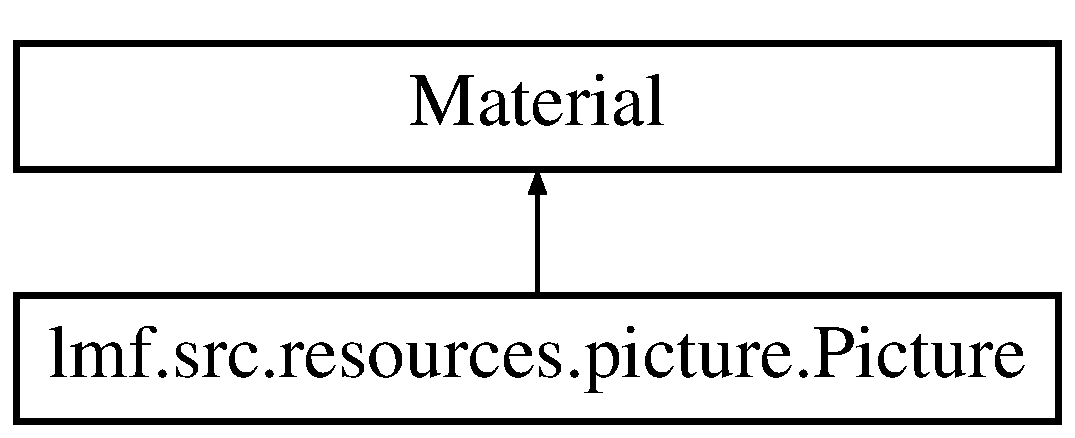
\includegraphics[height=2.000000cm]{classlmf_1_1src_1_1resources_1_1picture_1_1_picture}
\end{center}
\end{figure}
\subsection*{Public Member Functions}
\begin{DoxyCompactItemize}
\item 
def \hyperlink{classlmf_1_1src_1_1resources_1_1picture_1_1_picture_a32a8f644e3c068d7e0e904ba6a484aa8}{\+\_\+\+\_\+init\+\_\+\+\_\+}
\begin{DoxyCompactList}\small\item\em Constructor. \end{DoxyCompactList}\item 
def \hyperlink{classlmf_1_1src_1_1resources_1_1picture_1_1_picture_a9d1e78c17997e8cb029094adaffc904a}{\+\_\+\+\_\+del\+\_\+\+\_\+}
\begin{DoxyCompactList}\small\item\em Destructor. \end{DoxyCompactList}\end{DoxyCompactItemize}
\subsection*{Public Attributes}
\begin{DoxyCompactItemize}
\item 
\hyperlink{classlmf_1_1src_1_1resources_1_1picture_1_1_picture_a669715ddfa35b08171c493ac8f0b4468}{filename}
\item 
\hyperlink{classlmf_1_1src_1_1resources_1_1picture_1_1_picture_a0363561d74da7f2fd08b13b8b27c36cb}{reference}
\item 
\hyperlink{classlmf_1_1src_1_1resources_1_1picture_1_1_picture_a1611f370dd4b978d9ed7a0352bc79156}{width}
\item 
\hyperlink{classlmf_1_1src_1_1resources_1_1picture_1_1_picture_aac1448966226ee0d40b4aa756c33f7f8}{height}
\item 
\hyperlink{classlmf_1_1src_1_1resources_1_1picture_1_1_picture_a47e1b58864e999a59dbeb80fdf779238}{format}
\item 
\hyperlink{classlmf_1_1src_1_1resources_1_1picture_1_1_picture_ac9b506362a054a04c2dfc776ba853762}{statement}
\begin{DoxyCompactList}\small\item\em Statement instances are owned by \hyperlink{classlmf_1_1src_1_1resources_1_1picture_1_1_picture}{Picture} There is zero to many Statement instances per \hyperlink{classlmf_1_1src_1_1resources_1_1picture_1_1_picture}{Picture}. \end{DoxyCompactList}\end{DoxyCompactItemize}


\subsection{Detailed Description}
\hyperlink{classlmf_1_1src_1_1resources_1_1picture_1_1_picture}{Picture} is a Material subclass representing a picture. 

Definition at line 8 of file picture.\+py.



\subsection{Constructor \& Destructor Documentation}
\hypertarget{classlmf_1_1src_1_1resources_1_1picture_1_1_picture_a32a8f644e3c068d7e0e904ba6a484aa8}{\index{lmf\+::src\+::resources\+::picture\+::\+Picture@{lmf\+::src\+::resources\+::picture\+::\+Picture}!\+\_\+\+\_\+init\+\_\+\+\_\+@{\+\_\+\+\_\+init\+\_\+\+\_\+}}
\index{\+\_\+\+\_\+init\+\_\+\+\_\+@{\+\_\+\+\_\+init\+\_\+\+\_\+}!lmf\+::src\+::resources\+::picture\+::\+Picture@{lmf\+::src\+::resources\+::picture\+::\+Picture}}
\subsubsection[{\+\_\+\+\_\+init\+\_\+\+\_\+}]{\setlength{\rightskip}{0pt plus 5cm}def lmf.\+src.\+resources.\+picture.\+Picture.\+\_\+\+\_\+init\+\_\+\+\_\+ (
\begin{DoxyParamCaption}
\item[{}]{self}
\end{DoxyParamCaption}
)}}\label{classlmf_1_1src_1_1resources_1_1picture_1_1_picture_a32a8f644e3c068d7e0e904ba6a484aa8}


Constructor. 

\hyperlink{classlmf_1_1src_1_1resources_1_1picture_1_1_picture}{Picture} instances are owned by ?. \begin{DoxyReturn}{Returns}
A \hyperlink{classlmf_1_1src_1_1resources_1_1picture_1_1_picture}{Picture} instance. 
\end{DoxyReturn}


Definition at line 11 of file picture.\+py.

\hypertarget{classlmf_1_1src_1_1resources_1_1picture_1_1_picture_a9d1e78c17997e8cb029094adaffc904a}{\index{lmf\+::src\+::resources\+::picture\+::\+Picture@{lmf\+::src\+::resources\+::picture\+::\+Picture}!\+\_\+\+\_\+del\+\_\+\+\_\+@{\+\_\+\+\_\+del\+\_\+\+\_\+}}
\index{\+\_\+\+\_\+del\+\_\+\+\_\+@{\+\_\+\+\_\+del\+\_\+\+\_\+}!lmf\+::src\+::resources\+::picture\+::\+Picture@{lmf\+::src\+::resources\+::picture\+::\+Picture}}
\subsubsection[{\+\_\+\+\_\+del\+\_\+\+\_\+}]{\setlength{\rightskip}{0pt plus 5cm}def lmf.\+src.\+resources.\+picture.\+Picture.\+\_\+\+\_\+del\+\_\+\+\_\+ (
\begin{DoxyParamCaption}
\item[{}]{self}
\end{DoxyParamCaption}
)}}\label{classlmf_1_1src_1_1resources_1_1picture_1_1_picture_a9d1e78c17997e8cb029094adaffc904a}


Destructor. 

Release Statement instances. 

Definition at line 27 of file picture.\+py.



\subsection{Member Data Documentation}
\hypertarget{classlmf_1_1src_1_1resources_1_1picture_1_1_picture_a669715ddfa35b08171c493ac8f0b4468}{\index{lmf\+::src\+::resources\+::picture\+::\+Picture@{lmf\+::src\+::resources\+::picture\+::\+Picture}!filename@{filename}}
\index{filename@{filename}!lmf\+::src\+::resources\+::picture\+::\+Picture@{lmf\+::src\+::resources\+::picture\+::\+Picture}}
\subsubsection[{filename}]{\setlength{\rightskip}{0pt plus 5cm}lmf.\+src.\+resources.\+picture.\+Picture.\+filename}}\label{classlmf_1_1src_1_1resources_1_1picture_1_1_picture_a669715ddfa35b08171c493ac8f0b4468}


Definition at line 18 of file picture.\+py.

\hypertarget{classlmf_1_1src_1_1resources_1_1picture_1_1_picture_a47e1b58864e999a59dbeb80fdf779238}{\index{lmf\+::src\+::resources\+::picture\+::\+Picture@{lmf\+::src\+::resources\+::picture\+::\+Picture}!format@{format}}
\index{format@{format}!lmf\+::src\+::resources\+::picture\+::\+Picture@{lmf\+::src\+::resources\+::picture\+::\+Picture}}
\subsubsection[{format}]{\setlength{\rightskip}{0pt plus 5cm}lmf.\+src.\+resources.\+picture.\+Picture.\+format}}\label{classlmf_1_1src_1_1resources_1_1picture_1_1_picture_a47e1b58864e999a59dbeb80fdf779238}


Definition at line 22 of file picture.\+py.

\hypertarget{classlmf_1_1src_1_1resources_1_1picture_1_1_picture_aac1448966226ee0d40b4aa756c33f7f8}{\index{lmf\+::src\+::resources\+::picture\+::\+Picture@{lmf\+::src\+::resources\+::picture\+::\+Picture}!height@{height}}
\index{height@{height}!lmf\+::src\+::resources\+::picture\+::\+Picture@{lmf\+::src\+::resources\+::picture\+::\+Picture}}
\subsubsection[{height}]{\setlength{\rightskip}{0pt plus 5cm}lmf.\+src.\+resources.\+picture.\+Picture.\+height}}\label{classlmf_1_1src_1_1resources_1_1picture_1_1_picture_aac1448966226ee0d40b4aa756c33f7f8}


Definition at line 21 of file picture.\+py.

\hypertarget{classlmf_1_1src_1_1resources_1_1picture_1_1_picture_a0363561d74da7f2fd08b13b8b27c36cb}{\index{lmf\+::src\+::resources\+::picture\+::\+Picture@{lmf\+::src\+::resources\+::picture\+::\+Picture}!reference@{reference}}
\index{reference@{reference}!lmf\+::src\+::resources\+::picture\+::\+Picture@{lmf\+::src\+::resources\+::picture\+::\+Picture}}
\subsubsection[{reference}]{\setlength{\rightskip}{0pt plus 5cm}lmf.\+src.\+resources.\+picture.\+Picture.\+reference}}\label{classlmf_1_1src_1_1resources_1_1picture_1_1_picture_a0363561d74da7f2fd08b13b8b27c36cb}


Definition at line 19 of file picture.\+py.

\hypertarget{classlmf_1_1src_1_1resources_1_1picture_1_1_picture_ac9b506362a054a04c2dfc776ba853762}{\index{lmf\+::src\+::resources\+::picture\+::\+Picture@{lmf\+::src\+::resources\+::picture\+::\+Picture}!statement@{statement}}
\index{statement@{statement}!lmf\+::src\+::resources\+::picture\+::\+Picture@{lmf\+::src\+::resources\+::picture\+::\+Picture}}
\subsubsection[{statement}]{\setlength{\rightskip}{0pt plus 5cm}lmf.\+src.\+resources.\+picture.\+Picture.\+statement}}\label{classlmf_1_1src_1_1resources_1_1picture_1_1_picture_ac9b506362a054a04c2dfc776ba853762}


Statement instances are owned by \hyperlink{classlmf_1_1src_1_1resources_1_1picture_1_1_picture}{Picture} There is zero to many Statement instances per \hyperlink{classlmf_1_1src_1_1resources_1_1picture_1_1_picture}{Picture}. 



Definition at line 25 of file picture.\+py.

\hypertarget{classlmf_1_1src_1_1resources_1_1picture_1_1_picture_a1611f370dd4b978d9ed7a0352bc79156}{\index{lmf\+::src\+::resources\+::picture\+::\+Picture@{lmf\+::src\+::resources\+::picture\+::\+Picture}!width@{width}}
\index{width@{width}!lmf\+::src\+::resources\+::picture\+::\+Picture@{lmf\+::src\+::resources\+::picture\+::\+Picture}}
\subsubsection[{width}]{\setlength{\rightskip}{0pt plus 5cm}lmf.\+src.\+resources.\+picture.\+Picture.\+width}}\label{classlmf_1_1src_1_1resources_1_1picture_1_1_picture_a1611f370dd4b978d9ed7a0352bc79156}


Definition at line 20 of file picture.\+py.



The documentation for this class was generated from the following file\+:\begin{DoxyCompactItemize}
\item 
/\+Users/celine/\+Work/\+C\+N\+R\+S/workspace/\+Himal\+Co/dev/lib/lmf/src/resources/\hyperlink{picture_8py}{picture.\+py}\end{DoxyCompactItemize}

\hypertarget{classlmf_1_1src_1_1morphology_1_1related__form_1_1_related_form}{\section{lmf.\+src.\+morphology.\+related\+\_\+form.\+Related\+Form Class Reference}
\label{classlmf_1_1src_1_1morphology_1_1related__form_1_1_related_form}\index{lmf.\+src.\+morphology.\+related\+\_\+form.\+Related\+Form@{lmf.\+src.\+morphology.\+related\+\_\+form.\+Related\+Form}}
}


\char`\"{}\+Related Form is a Form subclass representing a word form or a morph that can be related to the Lexical Entry. There is no asumption that the Related Form is associated with the Sense class in the Lexical Entry.\char`\"{} (L\+M\+F)  


Inheritance diagram for lmf.\+src.\+morphology.\+related\+\_\+form.\+Related\+Form\+:\begin{figure}[H]
\begin{center}
\leavevmode
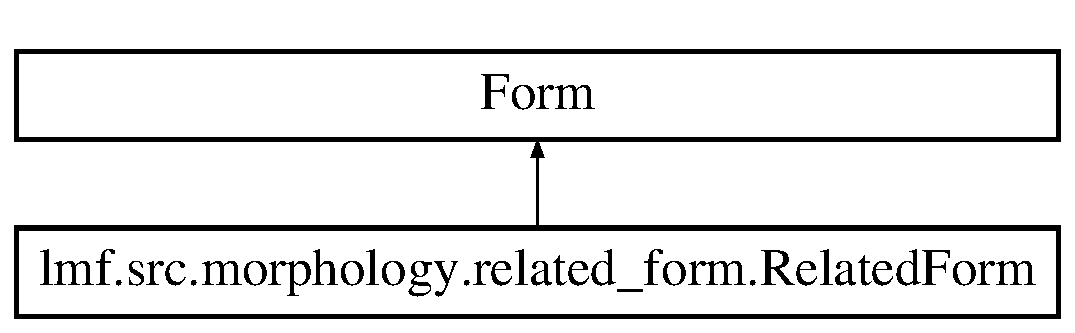
\includegraphics[height=2.000000cm]{classlmf_1_1src_1_1morphology_1_1related__form_1_1_related_form}
\end{center}
\end{figure}
\subsection*{Public Member Functions}
\begin{DoxyCompactItemize}
\item 
def \hyperlink{classlmf_1_1src_1_1morphology_1_1related__form_1_1_related_form_a241b3ec09b1802d10729f8fb4339300f}{\+\_\+\+\_\+init\+\_\+\+\_\+}
\begin{DoxyCompactList}\small\item\em Constructor. \end{DoxyCompactList}\item 
def \hyperlink{classlmf_1_1src_1_1morphology_1_1related__form_1_1_related_form_ae818d13f0783dafff76a95b4c1067e73}{\+\_\+\+\_\+del\+\_\+\+\_\+}
\begin{DoxyCompactList}\small\item\em Destructor. \end{DoxyCompactList}\item 
def \hyperlink{classlmf_1_1src_1_1morphology_1_1related__form_1_1_related_form_aeed3632165ec647be92c3804b32d2086}{set\+\_\+semantic\+Relation}
\begin{DoxyCompactList}\small\item\em Set semantic relation. \end{DoxyCompactList}\item 
def \hyperlink{classlmf_1_1src_1_1morphology_1_1related__form_1_1_related_form_a6c3cee5a3774ff44e1655671c75fa416}{get\+\_\+semantic\+Relation}
\begin{DoxyCompactList}\small\item\em Get semantic relation. \end{DoxyCompactList}\item 
def \hyperlink{classlmf_1_1src_1_1morphology_1_1related__form_1_1_related_form_a59ce1027881334fbf401bb9ffdd038e2}{get\+\_\+lexeme}
\begin{DoxyCompactList}\small\item\em Get related Lexical\+Entry lexeme. \end{DoxyCompactList}\item 
def \hyperlink{classlmf_1_1src_1_1morphology_1_1related__form_1_1_related_form_a84a43a4e867995031989488d1b5e397b}{set\+\_\+lexical\+\_\+entry}
\begin{DoxyCompactList}\small\item\em Set pointer to the related lexical entry instance. \end{DoxyCompactList}\item 
def \hyperlink{classlmf_1_1src_1_1morphology_1_1related__form_1_1_related_form_a851db32ef1f30794cdb921778058bc38}{get\+\_\+lexical\+\_\+entry}
\begin{DoxyCompactList}\small\item\em Get related Lexical\+Entry. \end{DoxyCompactList}\end{DoxyCompactItemize}
\subsection*{Public Attributes}
\begin{DoxyCompactItemize}
\item 
\hyperlink{classlmf_1_1src_1_1morphology_1_1related__form_1_1_related_form_a55ef34c7db0320aede2a86eff3085d46}{semantic\+Relation}
\item 
\hyperlink{classlmf_1_1src_1_1morphology_1_1related__form_1_1_related_form_a6f5035848e99af2cb539ba660d5c15a3}{targets}
\end{DoxyCompactItemize}


\subsection{Detailed Description}
\char`\"{}\+Related Form is a Form subclass representing a word form or a morph that can be related to the Lexical Entry. There is no asumption that the Related Form is associated with the Sense class in the Lexical Entry.\char`\"{} (L\+M\+F) 

Definition at line 11 of file related\+\_\+form.\+py.



\subsection{Constructor \& Destructor Documentation}
\hypertarget{classlmf_1_1src_1_1morphology_1_1related__form_1_1_related_form_a241b3ec09b1802d10729f8fb4339300f}{\index{lmf\+::src\+::morphology\+::related\+\_\+form\+::\+Related\+Form@{lmf\+::src\+::morphology\+::related\+\_\+form\+::\+Related\+Form}!\+\_\+\+\_\+init\+\_\+\+\_\+@{\+\_\+\+\_\+init\+\_\+\+\_\+}}
\index{\+\_\+\+\_\+init\+\_\+\+\_\+@{\+\_\+\+\_\+init\+\_\+\+\_\+}!lmf\+::src\+::morphology\+::related\+\_\+form\+::\+Related\+Form@{lmf\+::src\+::morphology\+::related\+\_\+form\+::\+Related\+Form}}
\subsubsection[{\+\_\+\+\_\+init\+\_\+\+\_\+}]{\setlength{\rightskip}{0pt plus 5cm}def lmf.\+src.\+morphology.\+related\+\_\+form.\+Related\+Form.\+\_\+\+\_\+init\+\_\+\+\_\+ (
\begin{DoxyParamCaption}
\item[{}]{self, }
\item[{}]{lexeme = {\ttfamily None}}
\end{DoxyParamCaption}
)}}\label{classlmf_1_1src_1_1morphology_1_1related__form_1_1_related_form_a241b3ec09b1802d10729f8fb4339300f}


Constructor. 

\hyperlink{classlmf_1_1src_1_1morphology_1_1related__form_1_1_related_form}{Related\+Form} instances are owned by Lexical\+Entry. 
\begin{DoxyParams}{Parameters}
{\em lexeme} & Related lexeme. If not provided, default value is None. \\
\hline
\end{DoxyParams}
\begin{DoxyReturn}{Returns}
A \hyperlink{classlmf_1_1src_1_1morphology_1_1related__form_1_1_related_form}{Related\+Form} instance. 
\end{DoxyReturn}


Definition at line 14 of file related\+\_\+form.\+py.

\hypertarget{classlmf_1_1src_1_1morphology_1_1related__form_1_1_related_form_ae818d13f0783dafff76a95b4c1067e73}{\index{lmf\+::src\+::morphology\+::related\+\_\+form\+::\+Related\+Form@{lmf\+::src\+::morphology\+::related\+\_\+form\+::\+Related\+Form}!\+\_\+\+\_\+del\+\_\+\+\_\+@{\+\_\+\+\_\+del\+\_\+\+\_\+}}
\index{\+\_\+\+\_\+del\+\_\+\+\_\+@{\+\_\+\+\_\+del\+\_\+\+\_\+}!lmf\+::src\+::morphology\+::related\+\_\+form\+::\+Related\+Form@{lmf\+::src\+::morphology\+::related\+\_\+form\+::\+Related\+Form}}
\subsubsection[{\+\_\+\+\_\+del\+\_\+\+\_\+}]{\setlength{\rightskip}{0pt plus 5cm}def lmf.\+src.\+morphology.\+related\+\_\+form.\+Related\+Form.\+\_\+\+\_\+del\+\_\+\+\_\+ (
\begin{DoxyParamCaption}
\item[{}]{self}
\end{DoxyParamCaption}
)}}\label{classlmf_1_1src_1_1morphology_1_1related__form_1_1_related_form_ae818d13f0783dafff76a95b4c1067e73}


Destructor. 



Definition at line 29 of file related\+\_\+form.\+py.



\subsection{Member Function Documentation}
\hypertarget{classlmf_1_1src_1_1morphology_1_1related__form_1_1_related_form_a59ce1027881334fbf401bb9ffdd038e2}{\index{lmf\+::src\+::morphology\+::related\+\_\+form\+::\+Related\+Form@{lmf\+::src\+::morphology\+::related\+\_\+form\+::\+Related\+Form}!get\+\_\+lexeme@{get\+\_\+lexeme}}
\index{get\+\_\+lexeme@{get\+\_\+lexeme}!lmf\+::src\+::morphology\+::related\+\_\+form\+::\+Related\+Form@{lmf\+::src\+::morphology\+::related\+\_\+form\+::\+Related\+Form}}
\subsubsection[{get\+\_\+lexeme}]{\setlength{\rightskip}{0pt plus 5cm}def lmf.\+src.\+morphology.\+related\+\_\+form.\+Related\+Form.\+get\+\_\+lexeme (
\begin{DoxyParamCaption}
\item[{}]{self}
\end{DoxyParamCaption}
)}}\label{classlmf_1_1src_1_1morphology_1_1related__form_1_1_related_form_a59ce1027881334fbf401bb9ffdd038e2}


Get related Lexical\+Entry lexeme. 

\begin{DoxyReturn}{Returns}
\hyperlink{classlmf_1_1src_1_1morphology_1_1related__form_1_1_related_form}{Related\+Form} attribute 'targets'. 
\end{DoxyReturn}


Definition at line 54 of file related\+\_\+form.\+py.

\hypertarget{classlmf_1_1src_1_1morphology_1_1related__form_1_1_related_form_a851db32ef1f30794cdb921778058bc38}{\index{lmf\+::src\+::morphology\+::related\+\_\+form\+::\+Related\+Form@{lmf\+::src\+::morphology\+::related\+\_\+form\+::\+Related\+Form}!get\+\_\+lexical\+\_\+entry@{get\+\_\+lexical\+\_\+entry}}
\index{get\+\_\+lexical\+\_\+entry@{get\+\_\+lexical\+\_\+entry}!lmf\+::src\+::morphology\+::related\+\_\+form\+::\+Related\+Form@{lmf\+::src\+::morphology\+::related\+\_\+form\+::\+Related\+Form}}
\subsubsection[{get\+\_\+lexical\+\_\+entry}]{\setlength{\rightskip}{0pt plus 5cm}def lmf.\+src.\+morphology.\+related\+\_\+form.\+Related\+Form.\+get\+\_\+lexical\+\_\+entry (
\begin{DoxyParamCaption}
\item[{}]{self}
\end{DoxyParamCaption}
)}}\label{classlmf_1_1src_1_1morphology_1_1related__form_1_1_related_form_a851db32ef1f30794cdb921778058bc38}


Get related Lexical\+Entry. 

\begin{DoxyReturn}{Returns}
\hyperlink{classlmf_1_1src_1_1morphology_1_1related__form_1_1_related_form}{Related\+Form} private attribute '\+\_\+\+\_\+lexical\+\_\+entry'. 
\end{DoxyReturn}


Definition at line 68 of file related\+\_\+form.\+py.

\hypertarget{classlmf_1_1src_1_1morphology_1_1related__form_1_1_related_form_a6c3cee5a3774ff44e1655671c75fa416}{\index{lmf\+::src\+::morphology\+::related\+\_\+form\+::\+Related\+Form@{lmf\+::src\+::morphology\+::related\+\_\+form\+::\+Related\+Form}!get\+\_\+semantic\+Relation@{get\+\_\+semantic\+Relation}}
\index{get\+\_\+semantic\+Relation@{get\+\_\+semantic\+Relation}!lmf\+::src\+::morphology\+::related\+\_\+form\+::\+Related\+Form@{lmf\+::src\+::morphology\+::related\+\_\+form\+::\+Related\+Form}}
\subsubsection[{get\+\_\+semantic\+Relation}]{\setlength{\rightskip}{0pt plus 5cm}def lmf.\+src.\+morphology.\+related\+\_\+form.\+Related\+Form.\+get\+\_\+semantic\+Relation (
\begin{DoxyParamCaption}
\item[{}]{self}
\end{DoxyParamCaption}
)}}\label{classlmf_1_1src_1_1morphology_1_1related__form_1_1_related_form_a6c3cee5a3774ff44e1655671c75fa416}


Get semantic relation. 

\begin{DoxyReturn}{Returns}
\hyperlink{classlmf_1_1src_1_1morphology_1_1related__form_1_1_related_form}{Related\+Form} attribute 'semantic\+Relation'. 
\end{DoxyReturn}


Definition at line 48 of file related\+\_\+form.\+py.

\hypertarget{classlmf_1_1src_1_1morphology_1_1related__form_1_1_related_form_a84a43a4e867995031989488d1b5e397b}{\index{lmf\+::src\+::morphology\+::related\+\_\+form\+::\+Related\+Form@{lmf\+::src\+::morphology\+::related\+\_\+form\+::\+Related\+Form}!set\+\_\+lexical\+\_\+entry@{set\+\_\+lexical\+\_\+entry}}
\index{set\+\_\+lexical\+\_\+entry@{set\+\_\+lexical\+\_\+entry}!lmf\+::src\+::morphology\+::related\+\_\+form\+::\+Related\+Form@{lmf\+::src\+::morphology\+::related\+\_\+form\+::\+Related\+Form}}
\subsubsection[{set\+\_\+lexical\+\_\+entry}]{\setlength{\rightskip}{0pt plus 5cm}def lmf.\+src.\+morphology.\+related\+\_\+form.\+Related\+Form.\+set\+\_\+lexical\+\_\+entry (
\begin{DoxyParamCaption}
\item[{}]{self, }
\item[{}]{lexical\+\_\+entry}
\end{DoxyParamCaption}
)}}\label{classlmf_1_1src_1_1morphology_1_1related__form_1_1_related_form_a84a43a4e867995031989488d1b5e397b}


Set pointer to the related lexical entry instance. 

This function can only be called once the full dictionary has been parsed. 
\begin{DoxyParams}{Parameters}
{\em lexical\+\_\+entry} & The related Lexical\+Entry. \\
\hline
\end{DoxyParams}
\begin{DoxyReturn}{Returns}
\hyperlink{classlmf_1_1src_1_1morphology_1_1related__form_1_1_related_form}{Related\+Form} instance. 
\end{DoxyReturn}


Definition at line 60 of file related\+\_\+form.\+py.

\hypertarget{classlmf_1_1src_1_1morphology_1_1related__form_1_1_related_form_aeed3632165ec647be92c3804b32d2086}{\index{lmf\+::src\+::morphology\+::related\+\_\+form\+::\+Related\+Form@{lmf\+::src\+::morphology\+::related\+\_\+form\+::\+Related\+Form}!set\+\_\+semantic\+Relation@{set\+\_\+semantic\+Relation}}
\index{set\+\_\+semantic\+Relation@{set\+\_\+semantic\+Relation}!lmf\+::src\+::morphology\+::related\+\_\+form\+::\+Related\+Form@{lmf\+::src\+::morphology\+::related\+\_\+form\+::\+Related\+Form}}
\subsubsection[{set\+\_\+semantic\+Relation}]{\setlength{\rightskip}{0pt plus 5cm}def lmf.\+src.\+morphology.\+related\+\_\+form.\+Related\+Form.\+set\+\_\+semantic\+Relation (
\begin{DoxyParamCaption}
\item[{}]{self, }
\item[{}]{semantic\+\_\+relation}
\end{DoxyParamCaption}
)}}\label{classlmf_1_1src_1_1morphology_1_1related__form_1_1_related_form_aeed3632165ec647be92c3804b32d2086}


Set semantic relation. 


\begin{DoxyParams}{Parameters}
{\em semantic\+\_\+relation} & The semantic relation to set. \\
\hline
\end{DoxyParams}
\begin{DoxyReturn}{Returns}
\hyperlink{classlmf_1_1src_1_1morphology_1_1related__form_1_1_related_form}{Related\+Form} instance. 
\end{DoxyReturn}


Definition at line 35 of file related\+\_\+form.\+py.



\subsection{Member Data Documentation}
\hypertarget{classlmf_1_1src_1_1morphology_1_1related__form_1_1_related_form_a55ef34c7db0320aede2a86eff3085d46}{\index{lmf\+::src\+::morphology\+::related\+\_\+form\+::\+Related\+Form@{lmf\+::src\+::morphology\+::related\+\_\+form\+::\+Related\+Form}!semantic\+Relation@{semantic\+Relation}}
\index{semantic\+Relation@{semantic\+Relation}!lmf\+::src\+::morphology\+::related\+\_\+form\+::\+Related\+Form@{lmf\+::src\+::morphology\+::related\+\_\+form\+::\+Related\+Form}}
\subsubsection[{semantic\+Relation}]{\setlength{\rightskip}{0pt plus 5cm}lmf.\+src.\+morphology.\+related\+\_\+form.\+Related\+Form.\+semantic\+Relation}}\label{classlmf_1_1src_1_1morphology_1_1related__form_1_1_related_form_a55ef34c7db0320aede2a86eff3085d46}


Definition at line 22 of file related\+\_\+form.\+py.

\hypertarget{classlmf_1_1src_1_1morphology_1_1related__form_1_1_related_form_a6f5035848e99af2cb539ba660d5c15a3}{\index{lmf\+::src\+::morphology\+::related\+\_\+form\+::\+Related\+Form@{lmf\+::src\+::morphology\+::related\+\_\+form\+::\+Related\+Form}!targets@{targets}}
\index{targets@{targets}!lmf\+::src\+::morphology\+::related\+\_\+form\+::\+Related\+Form@{lmf\+::src\+::morphology\+::related\+\_\+form\+::\+Related\+Form}}
\subsubsection[{targets}]{\setlength{\rightskip}{0pt plus 5cm}lmf.\+src.\+morphology.\+related\+\_\+form.\+Related\+Form.\+targets}}\label{classlmf_1_1src_1_1morphology_1_1related__form_1_1_related_form_a6f5035848e99af2cb539ba660d5c15a3}


Definition at line 24 of file related\+\_\+form.\+py.



The documentation for this class was generated from the following file\+:\begin{DoxyCompactItemize}
\item 
/\+Users/celine/\+Work/\+C\+N\+R\+S/workspace/\+Himal\+Co/dev/lib/lmf/src/morphology/\hyperlink{related__form_8py}{related\+\_\+form.\+py}\end{DoxyCompactItemize}

\hypertarget{classlmf_1_1src_1_1core_1_1representation_1_1_representation}{\section{lmf.\+src.\+core.\+representation.\+Representation Class Reference}
\label{classlmf_1_1src_1_1core_1_1representation_1_1_representation}\index{lmf.\+src.\+core.\+representation.\+Representation@{lmf.\+src.\+core.\+representation.\+Representation}}
}


\char`\"{}\+Representation class is an abstract class representing a Unicode string as well as, if needed, the unique attribute-\/value pairs that describe the specific language, script and orthography.\char`\"{} (L\+M\+F)  


\subsection*{Public Member Functions}
\begin{DoxyCompactItemize}
\item 
def \hyperlink{classlmf_1_1src_1_1core_1_1representation_1_1_representation_acd1be9562ebfd01660301f22ee57a50c}{\+\_\+\+\_\+init\+\_\+\+\_\+}
\begin{DoxyCompactList}\small\item\em As \hyperlink{classlmf_1_1src_1_1core_1_1representation_1_1_representation}{Representation} is an abstract class, constructor raises an error. \end{DoxyCompactList}\item 
def \hyperlink{classlmf_1_1src_1_1core_1_1representation_1_1_representation_aac0e09b6c37690ed70a51981cd5b251d}{\+\_\+\+\_\+del\+\_\+\+\_\+}
\begin{DoxyCompactList}\small\item\em As \hyperlink{classlmf_1_1src_1_1core_1_1representation_1_1_representation}{Representation} is an abstract class, desctructor raises an error. \end{DoxyCompactList}\item 
def \hyperlink{classlmf_1_1src_1_1core_1_1representation_1_1_representation_ac592206f4f5af84f6a03af40f36ebffa}{\+\_\+\+\_\+new\+\_\+\+\_\+}
\begin{DoxyCompactList}\small\item\em Private initialization called from \hyperlink{classlmf_1_1src_1_1core_1_1representation_1_1_representation}{Representation} subclasses. \end{DoxyCompactList}\end{DoxyCompactItemize}
\subsection*{Public Attributes}
\begin{DoxyCompactItemize}
\item 
\hyperlink{classlmf_1_1src_1_1core_1_1representation_1_1_representation_a3442469787d13456fbaf6e5ee79037d5}{comment}
\item 
\hyperlink{classlmf_1_1src_1_1core_1_1representation_1_1_representation_a3966cc4e61369fde0e86dda8a656a0e1}{written\+Form}
\item 
\hyperlink{classlmf_1_1src_1_1core_1_1representation_1_1_representation_afc9334b238179d0a79d3ce1e13d4d304}{language}
\item 
\hyperlink{classlmf_1_1src_1_1core_1_1representation_1_1_representation_a84dbae01d3e39cd1d4ac8d420372dce4}{script\+Name}
\end{DoxyCompactItemize}


\subsection{Detailed Description}
\char`\"{}\+Representation class is an abstract class representing a Unicode string as well as, if needed, the unique attribute-\/value pairs that describe the specific language, script and orthography.\char`\"{} (L\+M\+F) 

Definition at line 6 of file representation.\+py.



\subsection{Constructor \& Destructor Documentation}
\hypertarget{classlmf_1_1src_1_1core_1_1representation_1_1_representation_acd1be9562ebfd01660301f22ee57a50c}{\index{lmf\+::src\+::core\+::representation\+::\+Representation@{lmf\+::src\+::core\+::representation\+::\+Representation}!\+\_\+\+\_\+init\+\_\+\+\_\+@{\+\_\+\+\_\+init\+\_\+\+\_\+}}
\index{\+\_\+\+\_\+init\+\_\+\+\_\+@{\+\_\+\+\_\+init\+\_\+\+\_\+}!lmf\+::src\+::core\+::representation\+::\+Representation@{lmf\+::src\+::core\+::representation\+::\+Representation}}
\subsubsection[{\+\_\+\+\_\+init\+\_\+\+\_\+}]{\setlength{\rightskip}{0pt plus 5cm}def lmf.\+src.\+core.\+representation.\+Representation.\+\_\+\+\_\+init\+\_\+\+\_\+ (
\begin{DoxyParamCaption}
\item[{}]{self}
\end{DoxyParamCaption}
)}}\label{classlmf_1_1src_1_1core_1_1representation_1_1_representation_acd1be9562ebfd01660301f22ee57a50c}


As \hyperlink{classlmf_1_1src_1_1core_1_1representation_1_1_representation}{Representation} is an abstract class, constructor raises an error. 



Definition at line 9 of file representation.\+py.

\hypertarget{classlmf_1_1src_1_1core_1_1representation_1_1_representation_aac0e09b6c37690ed70a51981cd5b251d}{\index{lmf\+::src\+::core\+::representation\+::\+Representation@{lmf\+::src\+::core\+::representation\+::\+Representation}!\+\_\+\+\_\+del\+\_\+\+\_\+@{\+\_\+\+\_\+del\+\_\+\+\_\+}}
\index{\+\_\+\+\_\+del\+\_\+\+\_\+@{\+\_\+\+\_\+del\+\_\+\+\_\+}!lmf\+::src\+::core\+::representation\+::\+Representation@{lmf\+::src\+::core\+::representation\+::\+Representation}}
\subsubsection[{\+\_\+\+\_\+del\+\_\+\+\_\+}]{\setlength{\rightskip}{0pt plus 5cm}def lmf.\+src.\+core.\+representation.\+Representation.\+\_\+\+\_\+del\+\_\+\+\_\+ (
\begin{DoxyParamCaption}
\item[{}]{self}
\end{DoxyParamCaption}
)}}\label{classlmf_1_1src_1_1core_1_1representation_1_1_representation_aac0e09b6c37690ed70a51981cd5b251d}


As \hyperlink{classlmf_1_1src_1_1core_1_1representation_1_1_representation}{Representation} is an abstract class, desctructor raises an error. 



Definition at line 14 of file representation.\+py.



\subsection{Member Function Documentation}
\hypertarget{classlmf_1_1src_1_1core_1_1representation_1_1_representation_ac592206f4f5af84f6a03af40f36ebffa}{\index{lmf\+::src\+::core\+::representation\+::\+Representation@{lmf\+::src\+::core\+::representation\+::\+Representation}!\+\_\+\+\_\+new\+\_\+\+\_\+@{\+\_\+\+\_\+new\+\_\+\+\_\+}}
\index{\+\_\+\+\_\+new\+\_\+\+\_\+@{\+\_\+\+\_\+new\+\_\+\+\_\+}!lmf\+::src\+::core\+::representation\+::\+Representation@{lmf\+::src\+::core\+::representation\+::\+Representation}}
\subsubsection[{\+\_\+\+\_\+new\+\_\+\+\_\+}]{\setlength{\rightskip}{0pt plus 5cm}def lmf.\+src.\+core.\+representation.\+Representation.\+\_\+\+\_\+new\+\_\+\+\_\+ (
\begin{DoxyParamCaption}
\item[{}]{self}
\end{DoxyParamCaption}
)}}\label{classlmf_1_1src_1_1core_1_1representation_1_1_representation_ac592206f4f5af84f6a03af40f36ebffa}


Private initialization called from \hyperlink{classlmf_1_1src_1_1core_1_1representation_1_1_representation}{Representation} subclasses. 



Definition at line 19 of file representation.\+py.



\subsection{Member Data Documentation}
\hypertarget{classlmf_1_1src_1_1core_1_1representation_1_1_representation_a3442469787d13456fbaf6e5ee79037d5}{\index{lmf\+::src\+::core\+::representation\+::\+Representation@{lmf\+::src\+::core\+::representation\+::\+Representation}!comment@{comment}}
\index{comment@{comment}!lmf\+::src\+::core\+::representation\+::\+Representation@{lmf\+::src\+::core\+::representation\+::\+Representation}}
\subsubsection[{comment}]{\setlength{\rightskip}{0pt plus 5cm}lmf.\+src.\+core.\+representation.\+Representation.\+comment}}\label{classlmf_1_1src_1_1core_1_1representation_1_1_representation_a3442469787d13456fbaf6e5ee79037d5}


Definition at line 22 of file representation.\+py.

\hypertarget{classlmf_1_1src_1_1core_1_1representation_1_1_representation_afc9334b238179d0a79d3ce1e13d4d304}{\index{lmf\+::src\+::core\+::representation\+::\+Representation@{lmf\+::src\+::core\+::representation\+::\+Representation}!language@{language}}
\index{language@{language}!lmf\+::src\+::core\+::representation\+::\+Representation@{lmf\+::src\+::core\+::representation\+::\+Representation}}
\subsubsection[{language}]{\setlength{\rightskip}{0pt plus 5cm}lmf.\+src.\+core.\+representation.\+Representation.\+language}}\label{classlmf_1_1src_1_1core_1_1representation_1_1_representation_afc9334b238179d0a79d3ce1e13d4d304}


Definition at line 24 of file representation.\+py.

\hypertarget{classlmf_1_1src_1_1core_1_1representation_1_1_representation_a84dbae01d3e39cd1d4ac8d420372dce4}{\index{lmf\+::src\+::core\+::representation\+::\+Representation@{lmf\+::src\+::core\+::representation\+::\+Representation}!script\+Name@{script\+Name}}
\index{script\+Name@{script\+Name}!lmf\+::src\+::core\+::representation\+::\+Representation@{lmf\+::src\+::core\+::representation\+::\+Representation}}
\subsubsection[{script\+Name}]{\setlength{\rightskip}{0pt plus 5cm}lmf.\+src.\+core.\+representation.\+Representation.\+script\+Name}}\label{classlmf_1_1src_1_1core_1_1representation_1_1_representation_a84dbae01d3e39cd1d4ac8d420372dce4}


Definition at line 25 of file representation.\+py.

\hypertarget{classlmf_1_1src_1_1core_1_1representation_1_1_representation_a3966cc4e61369fde0e86dda8a656a0e1}{\index{lmf\+::src\+::core\+::representation\+::\+Representation@{lmf\+::src\+::core\+::representation\+::\+Representation}!written\+Form@{written\+Form}}
\index{written\+Form@{written\+Form}!lmf\+::src\+::core\+::representation\+::\+Representation@{lmf\+::src\+::core\+::representation\+::\+Representation}}
\subsubsection[{written\+Form}]{\setlength{\rightskip}{0pt plus 5cm}lmf.\+src.\+core.\+representation.\+Representation.\+written\+Form}}\label{classlmf_1_1src_1_1core_1_1representation_1_1_representation_a3966cc4e61369fde0e86dda8a656a0e1}


Definition at line 23 of file representation.\+py.



The documentation for this class was generated from the following file\+:\begin{DoxyCompactItemize}
\item 
/\+Users/celine/\+Work/\+C\+N\+R\+S/workspace/\+Himal\+Co/dev/lib/lmf/src/core/\hyperlink{representation_8py}{representation.\+py}\end{DoxyCompactItemize}

\hypertarget{classlmf_1_1src_1_1resources_1_1resource_1_1_resource}{\section{lmf.\+src.\+resources.\+resource.\+Resource Class Reference}
\label{classlmf_1_1src_1_1resources_1_1resource_1_1_resource}\index{lmf.\+src.\+resources.\+resource.\+Resource@{lmf.\+src.\+resources.\+resource.\+Resource}}
}


\hyperlink{classlmf_1_1src_1_1resources_1_1resource_1_1_resource}{Resource} is an abstract class representing a material or a human resource.  


\subsection*{Public Member Functions}
\begin{DoxyCompactItemize}
\item 
def \hyperlink{classlmf_1_1src_1_1resources_1_1resource_1_1_resource_adf841a9c1edc70040858112b7f144e3f}{\+\_\+\+\_\+init\+\_\+\+\_\+}
\begin{DoxyCompactList}\small\item\em As \hyperlink{classlmf_1_1src_1_1resources_1_1resource_1_1_resource}{Resource} is an abstract class, constructor raises an error. \end{DoxyCompactList}\item 
def \hyperlink{classlmf_1_1src_1_1resources_1_1resource_1_1_resource_af3f1ceb63eb841d5bc2ce20df9c74d7a}{\+\_\+\+\_\+del\+\_\+\+\_\+}
\begin{DoxyCompactList}\small\item\em As \hyperlink{classlmf_1_1src_1_1resources_1_1resource_1_1_resource}{Resource} is an abstract class, desctructor raises an error. \end{DoxyCompactList}\item 
def \hyperlink{classlmf_1_1src_1_1resources_1_1resource_1_1_resource_ae969204ff849acf51dcb4ae522d8914d}{\+\_\+\+\_\+call\+\_\+\+\_\+}
\begin{DoxyCompactList}\small\item\em Private initialization called from \hyperlink{classlmf_1_1src_1_1resources_1_1resource_1_1_resource}{Resource} subclasses. \end{DoxyCompactList}\end{DoxyCompactItemize}


\subsection{Detailed Description}
\hyperlink{classlmf_1_1src_1_1resources_1_1resource_1_1_resource}{Resource} is an abstract class representing a material or a human resource. 

The \hyperlink{classlmf_1_1src_1_1resources_1_1resource_1_1_resource}{Resource} class allows subclasses. 

Definition at line 6 of file resource.\+py.



\subsection{Constructor \& Destructor Documentation}
\hypertarget{classlmf_1_1src_1_1resources_1_1resource_1_1_resource_adf841a9c1edc70040858112b7f144e3f}{\index{lmf\+::src\+::resources\+::resource\+::\+Resource@{lmf\+::src\+::resources\+::resource\+::\+Resource}!\+\_\+\+\_\+init\+\_\+\+\_\+@{\+\_\+\+\_\+init\+\_\+\+\_\+}}
\index{\+\_\+\+\_\+init\+\_\+\+\_\+@{\+\_\+\+\_\+init\+\_\+\+\_\+}!lmf\+::src\+::resources\+::resource\+::\+Resource@{lmf\+::src\+::resources\+::resource\+::\+Resource}}
\subsubsection[{\+\_\+\+\_\+init\+\_\+\+\_\+}]{\setlength{\rightskip}{0pt plus 5cm}def lmf.\+src.\+resources.\+resource.\+Resource.\+\_\+\+\_\+init\+\_\+\+\_\+ (
\begin{DoxyParamCaption}
\item[{}]{self}
\end{DoxyParamCaption}
)}}\label{classlmf_1_1src_1_1resources_1_1resource_1_1_resource_adf841a9c1edc70040858112b7f144e3f}


As \hyperlink{classlmf_1_1src_1_1resources_1_1resource_1_1_resource}{Resource} is an abstract class, constructor raises an error. 



Definition at line 9 of file resource.\+py.

\hypertarget{classlmf_1_1src_1_1resources_1_1resource_1_1_resource_af3f1ceb63eb841d5bc2ce20df9c74d7a}{\index{lmf\+::src\+::resources\+::resource\+::\+Resource@{lmf\+::src\+::resources\+::resource\+::\+Resource}!\+\_\+\+\_\+del\+\_\+\+\_\+@{\+\_\+\+\_\+del\+\_\+\+\_\+}}
\index{\+\_\+\+\_\+del\+\_\+\+\_\+@{\+\_\+\+\_\+del\+\_\+\+\_\+}!lmf\+::src\+::resources\+::resource\+::\+Resource@{lmf\+::src\+::resources\+::resource\+::\+Resource}}
\subsubsection[{\+\_\+\+\_\+del\+\_\+\+\_\+}]{\setlength{\rightskip}{0pt plus 5cm}def lmf.\+src.\+resources.\+resource.\+Resource.\+\_\+\+\_\+del\+\_\+\+\_\+ (
\begin{DoxyParamCaption}
\item[{}]{self}
\end{DoxyParamCaption}
)}}\label{classlmf_1_1src_1_1resources_1_1resource_1_1_resource_af3f1ceb63eb841d5bc2ce20df9c74d7a}


As \hyperlink{classlmf_1_1src_1_1resources_1_1resource_1_1_resource}{Resource} is an abstract class, desctructor raises an error. 



Definition at line 14 of file resource.\+py.



\subsection{Member Function Documentation}
\hypertarget{classlmf_1_1src_1_1resources_1_1resource_1_1_resource_ae969204ff849acf51dcb4ae522d8914d}{\index{lmf\+::src\+::resources\+::resource\+::\+Resource@{lmf\+::src\+::resources\+::resource\+::\+Resource}!\+\_\+\+\_\+call\+\_\+\+\_\+@{\+\_\+\+\_\+call\+\_\+\+\_\+}}
\index{\+\_\+\+\_\+call\+\_\+\+\_\+@{\+\_\+\+\_\+call\+\_\+\+\_\+}!lmf\+::src\+::resources\+::resource\+::\+Resource@{lmf\+::src\+::resources\+::resource\+::\+Resource}}
\subsubsection[{\+\_\+\+\_\+call\+\_\+\+\_\+}]{\setlength{\rightskip}{0pt plus 5cm}def lmf.\+src.\+resources.\+resource.\+Resource.\+\_\+\+\_\+call\+\_\+\+\_\+ (
\begin{DoxyParamCaption}
\item[{}]{self}
\end{DoxyParamCaption}
)}}\label{classlmf_1_1src_1_1resources_1_1resource_1_1_resource_ae969204ff849acf51dcb4ae522d8914d}


Private initialization called from \hyperlink{classlmf_1_1src_1_1resources_1_1resource_1_1_resource}{Resource} subclasses. 

\hyperlink{classlmf_1_1src_1_1resources_1_1resource_1_1_resource}{Resource} subinstances are owned by Lexical\+Resource. 

Definition at line 19 of file resource.\+py.



The documentation for this class was generated from the following file\+:\begin{DoxyCompactItemize}
\item 
/\+Users/celine/\+Work/\+C\+N\+R\+S/workspace/\+Himal\+Co/dev/lib/lmf/src/resources/\hyperlink{resource_8py}{resource.\+py}\end{DoxyCompactItemize}

\hypertarget{classlmf_1_1src_1_1core_1_1sense_1_1_sense}{\section{lmf.\+src.\+core.\+sense.\+Sense Class Reference}
\label{classlmf_1_1src_1_1core_1_1sense_1_1_sense}\index{lmf.\+src.\+core.\+sense.\+Sense@{lmf.\+src.\+core.\+sense.\+Sense}}
}


\char`\"{}\+Sense is a class representing one meaning of a lexical entry. The Sense class allows for hierarchical senses in that a sense may be more specific than another sense of the same lexical entry.\char`\"{} (L\+M\+F)  


\subsection*{Public Member Functions}
\begin{DoxyCompactItemize}
\item 
def \hyperlink{classlmf_1_1src_1_1core_1_1sense_1_1_sense_af0279b132d98c7b49141350ce34ea53b}{\+\_\+\+\_\+init\+\_\+\+\_\+}
\begin{DoxyCompactList}\small\item\em Constructor. \end{DoxyCompactList}\item 
def \hyperlink{classlmf_1_1src_1_1core_1_1sense_1_1_sense_a3cc439d56624626aaec6588dbcad5b58}{\+\_\+\+\_\+del\+\_\+\+\_\+}
\begin{DoxyCompactList}\small\item\em Destructor. \end{DoxyCompactList}\item 
def \hyperlink{classlmf_1_1src_1_1core_1_1sense_1_1_sense_aca94be206f4da6635798c1423aa5db15}{get\+\_\+id}
\begin{DoxyCompactList}\small\item\em I\+Dentifier. \end{DoxyCompactList}\item 
def \hyperlink{classlmf_1_1src_1_1core_1_1sense_1_1_sense_a144abbf38354979624e6b6902bd86cb7}{set\+\_\+sense\+Number}
\begin{DoxyCompactList}\small\item\em Set sense number. \end{DoxyCompactList}\item 
def \hyperlink{classlmf_1_1src_1_1core_1_1sense_1_1_sense_a0c1c636cbbcb1fd1e98e9f5058464d73}{get\+\_\+sense\+Number}
\begin{DoxyCompactList}\small\item\em Get sense number. \end{DoxyCompactList}\item 
def \hyperlink{classlmf_1_1src_1_1core_1_1sense_1_1_sense_a5923d173a0ad52642ccdc50d4611fdc9}{create\+\_\+definition}
\begin{DoxyCompactList}\small\item\em Create a definition. \end{DoxyCompactList}\item 
def \hyperlink{classlmf_1_1src_1_1core_1_1sense_1_1_sense_a28ac5eef8b1d952ee565792e56a1b748}{add\+\_\+definition}
\begin{DoxyCompactList}\small\item\em Add a definition to the sense. \end{DoxyCompactList}\item 
def \hyperlink{classlmf_1_1src_1_1core_1_1sense_1_1_sense_a8bc5ca5fd053360b3150a13fa7787528}{get\+\_\+definitions}
\begin{DoxyCompactList}\small\item\em Get all definitions maintained by the sense. \end{DoxyCompactList}\item 
def \hyperlink{classlmf_1_1src_1_1core_1_1sense_1_1_sense_a9b51914a3abc0ebfd57501a665a69eb2}{get\+\_\+last\+\_\+definition}
\begin{DoxyCompactList}\small\item\em Get the previously registered Definition instance. \end{DoxyCompactList}\item 
def \hyperlink{classlmf_1_1src_1_1core_1_1sense_1_1_sense_aef07a87a7893b5daea9b6a5a84220cab}{find\+\_\+definitions}
\begin{DoxyCompactList}\small\item\em Find definitions. \end{DoxyCompactList}\item 
def \hyperlink{classlmf_1_1src_1_1core_1_1sense_1_1_sense_a5a033c526c8b56d4ddf8f2f55ba45dec}{set\+\_\+definition}
\begin{DoxyCompactList}\small\item\em Set definition and language. \end{DoxyCompactList}\item 
def \hyperlink{classlmf_1_1src_1_1core_1_1sense_1_1_sense_a784fe796429c439fadd5e070954d70b3}{find\+\_\+glosses}
\begin{DoxyCompactList}\small\item\em Find glosses. \end{DoxyCompactList}\item 
def \hyperlink{classlmf_1_1src_1_1core_1_1sense_1_1_sense_a2a344e07bebb6d87f711b93ebf711fae}{set\+\_\+gloss}
\begin{DoxyCompactList}\small\item\em Set gloss and language. \end{DoxyCompactList}\item 
def \hyperlink{classlmf_1_1src_1_1core_1_1sense_1_1_sense_a0eadc746a37849a966279d1c35f687fe}{set\+\_\+note}
\begin{DoxyCompactList}\small\item\em Set note, note type and language. \end{DoxyCompactList}\item 
def \hyperlink{classlmf_1_1src_1_1core_1_1sense_1_1_sense_acc1067bd6d9a28ac2719d8d442a8d7bb}{find\+\_\+notes}
\begin{DoxyCompactList}\small\item\em Find notes. \end{DoxyCompactList}\item 
def \hyperlink{classlmf_1_1src_1_1core_1_1sense_1_1_sense_a9062f1b17bbc52c353edaf26330dcbeb}{set\+\_\+usage\+\_\+note}
\begin{DoxyCompactList}\small\item\em Set usage note and language. \end{DoxyCompactList}\item 
def \hyperlink{classlmf_1_1src_1_1core_1_1sense_1_1_sense_af4a689fe644baaf594abb4d9a1b0ca55}{find\+\_\+usage\+\_\+notes}
\begin{DoxyCompactList}\small\item\em Find usage notes. \end{DoxyCompactList}\item 
def \hyperlink{classlmf_1_1src_1_1core_1_1sense_1_1_sense_a99c9a5071df517bc60f33121d46c0db1}{set\+\_\+encyclopedic\+\_\+information}
\begin{DoxyCompactList}\small\item\em Set encyclopedic information and language. \end{DoxyCompactList}\item 
def \hyperlink{classlmf_1_1src_1_1core_1_1sense_1_1_sense_a7f3f74ce33b047118343b29c4a5196ce}{find\+\_\+encyclopedic\+\_\+informations}
\begin{DoxyCompactList}\small\item\em Find encyclopedic informations. \end{DoxyCompactList}\item 
def \hyperlink{classlmf_1_1src_1_1core_1_1sense_1_1_sense_a0ed9917e40d5be2e90d628b55f962ee8}{set\+\_\+restriction}
\begin{DoxyCompactList}\small\item\em Set restriction and language. \end{DoxyCompactList}\item 
def \hyperlink{classlmf_1_1src_1_1core_1_1sense_1_1_sense_ad2997077bd0e68f4af1542ade3e64417}{find\+\_\+restrictions}
\begin{DoxyCompactList}\small\item\em Find restrictions. \end{DoxyCompactList}\item 
def \hyperlink{classlmf_1_1src_1_1core_1_1sense_1_1_sense_a1174533bdabb24b077835ad384fb564c}{set\+\_\+borrowed\+\_\+word}
\begin{DoxyCompactList}\small\item\em Set source language (in English). \end{DoxyCompactList}\item 
def \hyperlink{classlmf_1_1src_1_1core_1_1sense_1_1_sense_a228d6a83808888d3805c06657c8f9153}{get\+\_\+borrowed\+\_\+word}
\begin{DoxyCompactList}\small\item\em Get source language (in English). \end{DoxyCompactList}\item 
def \hyperlink{classlmf_1_1src_1_1core_1_1sense_1_1_sense_adce959778963de3b295d05f81fa83390}{set\+\_\+written\+\_\+form}
\begin{DoxyCompactList}\small\item\em Set loan word. \end{DoxyCompactList}\item 
def \hyperlink{classlmf_1_1src_1_1core_1_1sense_1_1_sense_a06bf005156e07ed1262d53193bb75dc3}{get\+\_\+written\+\_\+form}
\begin{DoxyCompactList}\small\item\em Get loan word. \end{DoxyCompactList}\item 
def \hyperlink{classlmf_1_1src_1_1core_1_1sense_1_1_sense_a53537f8c8c41b7ad740fef272c9f8658}{set\+\_\+etymology}
\begin{DoxyCompactList}\small\item\em Set etymology. \end{DoxyCompactList}\item 
def \hyperlink{classlmf_1_1src_1_1core_1_1sense_1_1_sense_ae41863c9c5fdf94f3f29c13d6b1fe1cf}{get\+\_\+etymology}
\begin{DoxyCompactList}\small\item\em Get etymology. \end{DoxyCompactList}\item 
def \hyperlink{classlmf_1_1src_1_1core_1_1sense_1_1_sense_a621686bc8d18f6abd0f9a284f9c4b938}{set\+\_\+etymology\+\_\+comment}
\begin{DoxyCompactList}\small\item\em Set etymology comment and language. \end{DoxyCompactList}\item 
def \hyperlink{classlmf_1_1src_1_1core_1_1sense_1_1_sense_a60c30c7573483fd9d987c8c439688213}{get\+\_\+etymology\+\_\+comment}
\begin{DoxyCompactList}\small\item\em Get etymology comment. \end{DoxyCompactList}\item 
def \hyperlink{classlmf_1_1src_1_1core_1_1sense_1_1_sense_ab6f704b6dd461728169ffb3c74e43896}{get\+\_\+term\+\_\+source\+\_\+language}
\begin{DoxyCompactList}\small\item\em Get language used for the etymology comment. \end{DoxyCompactList}\item 
def \hyperlink{classlmf_1_1src_1_1core_1_1sense_1_1_sense_a2008e37c341cb4bb59bae4ed74bddef2}{set\+\_\+etymology\+\_\+gloss}
\begin{DoxyCompactList}\small\item\em Set etymology gloss. \end{DoxyCompactList}\item 
def \hyperlink{classlmf_1_1src_1_1core_1_1sense_1_1_sense_adb7c6fd2e19771361a94025df3343a58}{get\+\_\+etymology\+\_\+gloss}
\begin{DoxyCompactList}\small\item\em Get etymology gloss. \end{DoxyCompactList}\item 
def \hyperlink{classlmf_1_1src_1_1core_1_1sense_1_1_sense_ad869f9c4fcfca1775a74f6e1370c3476}{set\+\_\+etymology\+\_\+source}
\begin{DoxyCompactList}\small\item\em Set etymology source. \end{DoxyCompactList}\item 
def \hyperlink{classlmf_1_1src_1_1core_1_1sense_1_1_sense_a58b3a4780ebc7fec50bd5088fef02d87}{get\+\_\+etymology\+\_\+source}
\begin{DoxyCompactList}\small\item\em Get etymology source. \end{DoxyCompactList}\item 
def \hyperlink{classlmf_1_1src_1_1core_1_1sense_1_1_sense_ac61f3aadccb06f636aad9891b3bba53e}{create\+\_\+paradigm}
\begin{DoxyCompactList}\small\item\em Create a paradigm. \end{DoxyCompactList}\item 
def \hyperlink{classlmf_1_1src_1_1core_1_1sense_1_1_sense_ae67664c5b120e407e5d0543ad5bdfb3d}{add\+\_\+paradigm}
\begin{DoxyCompactList}\small\item\em Add a paradigm to the sense. \end{DoxyCompactList}\item 
def \hyperlink{classlmf_1_1src_1_1core_1_1sense_1_1_sense_a41112d70652f5412eb71eacad72a135a}{get\+\_\+paradigms}
\begin{DoxyCompactList}\small\item\em Get all paradigms maintained by the sense. \end{DoxyCompactList}\item 
def \hyperlink{classlmf_1_1src_1_1core_1_1sense_1_1_sense_abdb32f5050397be1f2147b769fc97f6d}{get\+\_\+last\+\_\+paradigm}
\begin{DoxyCompactList}\small\item\em Get the previously registered Paradigm instance. \end{DoxyCompactList}\item 
def \hyperlink{classlmf_1_1src_1_1core_1_1sense_1_1_sense_ab30230d0322d864c2222ba5471f1a305}{set\+\_\+paradigm\+\_\+label}
\begin{DoxyCompactList}\small\item\em Set paradigm label. \end{DoxyCompactList}\item 
def \hyperlink{classlmf_1_1src_1_1core_1_1sense_1_1_sense_abe2105eb98e2fc6349fa82965ad58261}{set\+\_\+paradigm\+\_\+form}
\begin{DoxyCompactList}\small\item\em Set paradigm form and language. \end{DoxyCompactList}\item 
def \hyperlink{classlmf_1_1src_1_1core_1_1sense_1_1_sense_a4b47011de018711098677f188e973fca}{set\+\_\+morphology}
\begin{DoxyCompactList}\small\item\em Set morphology. \end{DoxyCompactList}\item 
def \hyperlink{classlmf_1_1src_1_1core_1_1sense_1_1_sense_a14ced3b1dd8115d72283d6708d3ce0b5}{create\+\_\+and\+\_\+add\+\_\+context}
\begin{DoxyCompactList}\small\item\em Create a context and add it to the list. \end{DoxyCompactList}\item 
def \hyperlink{classlmf_1_1src_1_1core_1_1sense_1_1_sense_a50f6e0ba88d00c3315b91d3787aa9085}{get\+\_\+contexts}
\begin{DoxyCompactList}\small\item\em Get all contexts maintained by the sense. \end{DoxyCompactList}\item 
def \hyperlink{classlmf_1_1src_1_1core_1_1sense_1_1_sense_af9c1b79eed28bd28279719bdf578d218}{get\+\_\+last\+\_\+context}
\begin{DoxyCompactList}\small\item\em Get the previously registered Context instance. \end{DoxyCompactList}\item 
def \hyperlink{classlmf_1_1src_1_1core_1_1sense_1_1_sense_a61c046aabce91368de9129dd83c2bb20}{create\+\_\+example}
\begin{DoxyCompactList}\small\item\em Create a Context instance and set its written form and language. \end{DoxyCompactList}\item 
def \hyperlink{classlmf_1_1src_1_1core_1_1sense_1_1_sense_ab84c8d7a1cdcce014f99e0c1a1b0aedd}{add\+\_\+example}
\begin{DoxyCompactList}\small\item\em Set written form and language of an existing Context instance. \end{DoxyCompactList}\item 
def \hyperlink{classlmf_1_1src_1_1core_1_1sense_1_1_sense_a9b8d8ea7fe946dd19e2538fe7801754a}{set\+\_\+example\+\_\+comment}
\begin{DoxyCompactList}\small\item\em Set comment of an existing Context instance. \end{DoxyCompactList}\item 
def \hyperlink{classlmf_1_1src_1_1core_1_1sense_1_1_sense_a07d199aca70cf878cb2a71af7a96fa4c}{create\+\_\+and\+\_\+add\+\_\+subject\+\_\+field}
\begin{DoxyCompactList}\small\item\em Create a subject field and add it to the list. \end{DoxyCompactList}\item 
def \hyperlink{classlmf_1_1src_1_1core_1_1sense_1_1_sense_a907267d97926d04d20aaeefe475753d8}{get\+\_\+subject\+\_\+fields}
\begin{DoxyCompactList}\small\item\em Get all subject fields maintained by the sense. \end{DoxyCompactList}\item 
def \hyperlink{classlmf_1_1src_1_1core_1_1sense_1_1_sense_ad46f7e623293409ca06494b5fdeebe52}{set\+\_\+semantic\+\_\+domain}
\begin{DoxyCompactList}\small\item\em Create a Subject\+Field instance and set its semantic domain and language. \end{DoxyCompactList}\item 
def \hyperlink{classlmf_1_1src_1_1core_1_1sense_1_1_sense_a6004e31b078cad1d029283c4e3fedfc2}{create\+\_\+and\+\_\+add\+\_\+equivalent}
\begin{DoxyCompactList}\small\item\em Create an equivalent and add it to the list. \end{DoxyCompactList}\item 
def \hyperlink{classlmf_1_1src_1_1core_1_1sense_1_1_sense_ad01163c4440025fe86e4c00734aa8894}{get\+\_\+equivalents}
\begin{DoxyCompactList}\small\item\em Get all equivalents maintained by the sense. \end{DoxyCompactList}\item 
def \hyperlink{classlmf_1_1src_1_1core_1_1sense_1_1_sense_a97469fcc2116bb7b0dbf4826161512bd}{set\+\_\+translation}
\begin{DoxyCompactList}\small\item\em Create an Equivalent instance and set its translation and language. \end{DoxyCompactList}\item 
def \hyperlink{classlmf_1_1src_1_1core_1_1sense_1_1_sense_abeaa946d4c063f6784b84e443a102c2c}{get\+\_\+translations}
\begin{DoxyCompactList}\small\item\em Get all translations. \end{DoxyCompactList}\end{DoxyCompactItemize}
\subsection*{Public Attributes}
\begin{DoxyCompactItemize}
\item 
\hyperlink{classlmf_1_1src_1_1core_1_1sense_1_1_sense_ab511b70da3012cc5a0254f34dd30170c}{sense\+Number}
\item 
\hyperlink{classlmf_1_1src_1_1core_1_1sense_1_1_sense_ae0febecc9ab2951c5c6bb82f675187bc}{id}
\item 
\hyperlink{classlmf_1_1src_1_1core_1_1sense_1_1_sense_a9adfd8936ecd6626cba82193e068e09e}{definition}
\begin{DoxyCompactList}\small\item\em Definition instances are owned by \hyperlink{classlmf_1_1src_1_1core_1_1sense_1_1_sense}{Sense} There is zero to many Definition instances per \hyperlink{classlmf_1_1src_1_1core_1_1sense_1_1_sense}{Sense}. \end{DoxyCompactList}\item 
\hyperlink{classlmf_1_1src_1_1core_1_1sense_1_1_sense_a51524fd8eb1bc869c2ecfc681339d8aa}{sense}
\begin{DoxyCompactList}\small\item\em \hyperlink{classlmf_1_1src_1_1core_1_1sense_1_1_sense}{Sense} instances are owned by \hyperlink{classlmf_1_1src_1_1core_1_1sense_1_1_sense}{Sense} There is zero to many \hyperlink{classlmf_1_1src_1_1core_1_1sense_1_1_sense}{Sense} instances per \hyperlink{classlmf_1_1src_1_1core_1_1sense_1_1_sense}{Sense}. \end{DoxyCompactList}\item 
\hyperlink{classlmf_1_1src_1_1core_1_1sense_1_1_sense_a94d3b05f734fbe8898902ae948d30ce5}{equivalent}
\begin{DoxyCompactList}\small\item\em Equivalent instances are owned by \hyperlink{classlmf_1_1src_1_1core_1_1sense_1_1_sense}{Sense} There is zero to many Equivalent instances per \hyperlink{classlmf_1_1src_1_1core_1_1sense_1_1_sense}{Sense}. \end{DoxyCompactList}\item 
\hyperlink{classlmf_1_1src_1_1core_1_1sense_1_1_sense_ae2b3da0233748116d4415cc107b6e4c2}{context}
\begin{DoxyCompactList}\small\item\em Context instances are owned by \hyperlink{classlmf_1_1src_1_1core_1_1sense_1_1_sense}{Sense} There is zero to many Context instances per \hyperlink{classlmf_1_1src_1_1core_1_1sense_1_1_sense}{Sense}. \end{DoxyCompactList}\item 
\hyperlink{classlmf_1_1src_1_1core_1_1sense_1_1_sense_a1a7524732c66093f7156792292d3c9c3}{subject\+\_\+field}
\begin{DoxyCompactList}\small\item\em Subject\+Field instances are owned by \hyperlink{classlmf_1_1src_1_1core_1_1sense_1_1_sense}{Sense} There is zero to many Subject\+Field instances per \hyperlink{classlmf_1_1src_1_1core_1_1sense_1_1_sense}{Sense}. \end{DoxyCompactList}\item 
\hyperlink{classlmf_1_1src_1_1core_1_1sense_1_1_sense_a3f36a95173e4d4e7244e407a725dd3a9}{paradigm}
\begin{DoxyCompactList}\small\item\em Paradigm instances are owned by \hyperlink{classlmf_1_1src_1_1core_1_1sense_1_1_sense}{Sense} There is zero to many Paradigm instances per \hyperlink{classlmf_1_1src_1_1core_1_1sense_1_1_sense}{Sense}. \end{DoxyCompactList}\end{DoxyCompactItemize}


\subsection{Detailed Description}
\char`\"{}\+Sense is a class representing one meaning of a lexical entry. The Sense class allows for hierarchical senses in that a sense may be more specific than another sense of the same lexical entry.\char`\"{} (L\+M\+F) 

Definition at line 12 of file sense.\+py.



\subsection{Constructor \& Destructor Documentation}
\hypertarget{classlmf_1_1src_1_1core_1_1sense_1_1_sense_af0279b132d98c7b49141350ce34ea53b}{\index{lmf\+::src\+::core\+::sense\+::\+Sense@{lmf\+::src\+::core\+::sense\+::\+Sense}!\+\_\+\+\_\+init\+\_\+\+\_\+@{\+\_\+\+\_\+init\+\_\+\+\_\+}}
\index{\+\_\+\+\_\+init\+\_\+\+\_\+@{\+\_\+\+\_\+init\+\_\+\+\_\+}!lmf\+::src\+::core\+::sense\+::\+Sense@{lmf\+::src\+::core\+::sense\+::\+Sense}}
\subsubsection[{\+\_\+\+\_\+init\+\_\+\+\_\+}]{\setlength{\rightskip}{0pt plus 5cm}def lmf.\+src.\+core.\+sense.\+Sense.\+\_\+\+\_\+init\+\_\+\+\_\+ (
\begin{DoxyParamCaption}
\item[{}]{self, }
\item[{}]{id = {\ttfamily 0}}
\end{DoxyParamCaption}
)}}\label{classlmf_1_1src_1_1core_1_1sense_1_1_sense_af0279b132d98c7b49141350ce34ea53b}


Constructor. 

\hyperlink{classlmf_1_1src_1_1core_1_1sense_1_1_sense}{Sense} instances are owned by Lexical\+Entry. 
\begin{DoxyParams}{Parameters}
{\em id} & I\+Dentifier. If not provided, default value is 0. \\
\hline
\end{DoxyParams}
\begin{DoxyReturn}{Returns}
A \hyperlink{classlmf_1_1src_1_1core_1_1sense_1_1_sense}{Sense} instance. 
\end{DoxyReturn}


Definition at line 15 of file sense.\+py.

\hypertarget{classlmf_1_1src_1_1core_1_1sense_1_1_sense_a3cc439d56624626aaec6588dbcad5b58}{\index{lmf\+::src\+::core\+::sense\+::\+Sense@{lmf\+::src\+::core\+::sense\+::\+Sense}!\+\_\+\+\_\+del\+\_\+\+\_\+@{\+\_\+\+\_\+del\+\_\+\+\_\+}}
\index{\+\_\+\+\_\+del\+\_\+\+\_\+@{\+\_\+\+\_\+del\+\_\+\+\_\+}!lmf\+::src\+::core\+::sense\+::\+Sense@{lmf\+::src\+::core\+::sense\+::\+Sense}}
\subsubsection[{\+\_\+\+\_\+del\+\_\+\+\_\+}]{\setlength{\rightskip}{0pt plus 5cm}def lmf.\+src.\+core.\+sense.\+Sense.\+\_\+\+\_\+del\+\_\+\+\_\+ (
\begin{DoxyParamCaption}
\item[{}]{self}
\end{DoxyParamCaption}
)}}\label{classlmf_1_1src_1_1core_1_1sense_1_1_sense_a3cc439d56624626aaec6588dbcad5b58}


Destructor. 

Release Definition, \hyperlink{classlmf_1_1src_1_1core_1_1sense_1_1_sense}{Sense}, Equivalent, Context, Subject\+Field, Paradigm instances. 

Definition at line 43 of file sense.\+py.



\subsection{Member Function Documentation}
\hypertarget{classlmf_1_1src_1_1core_1_1sense_1_1_sense_a28ac5eef8b1d952ee565792e56a1b748}{\index{lmf\+::src\+::core\+::sense\+::\+Sense@{lmf\+::src\+::core\+::sense\+::\+Sense}!add\+\_\+definition@{add\+\_\+definition}}
\index{add\+\_\+definition@{add\+\_\+definition}!lmf\+::src\+::core\+::sense\+::\+Sense@{lmf\+::src\+::core\+::sense\+::\+Sense}}
\subsubsection[{add\+\_\+definition}]{\setlength{\rightskip}{0pt plus 5cm}def lmf.\+src.\+core.\+sense.\+Sense.\+add\+\_\+definition (
\begin{DoxyParamCaption}
\item[{}]{self, }
\item[{}]{definition}
\end{DoxyParamCaption}
)}}\label{classlmf_1_1src_1_1core_1_1sense_1_1_sense_a28ac5eef8b1d952ee565792e56a1b748}


Add a definition to the sense. 


\begin{DoxyParams}{Parameters}
{\em definition} & The Definition instance to add to the sense. \\
\hline
\end{DoxyParams}
\begin{DoxyReturn}{Returns}
\hyperlink{classlmf_1_1src_1_1core_1_1sense_1_1_sense}{Sense} instance. 
\end{DoxyReturn}


Definition at line 92 of file sense.\+py.

\hypertarget{classlmf_1_1src_1_1core_1_1sense_1_1_sense_ab84c8d7a1cdcce014f99e0c1a1b0aedd}{\index{lmf\+::src\+::core\+::sense\+::\+Sense@{lmf\+::src\+::core\+::sense\+::\+Sense}!add\+\_\+example@{add\+\_\+example}}
\index{add\+\_\+example@{add\+\_\+example}!lmf\+::src\+::core\+::sense\+::\+Sense@{lmf\+::src\+::core\+::sense\+::\+Sense}}
\subsubsection[{add\+\_\+example}]{\setlength{\rightskip}{0pt plus 5cm}def lmf.\+src.\+core.\+sense.\+Sense.\+add\+\_\+example (
\begin{DoxyParamCaption}
\item[{}]{self, }
\item[{}]{written\+\_\+form, }
\item[{}]{language = {\ttfamily None}}
\end{DoxyParamCaption}
)}}\label{classlmf_1_1src_1_1core_1_1sense_1_1_sense_ab84c8d7a1cdcce014f99e0c1a1b0aedd}


Set written form and language of an existing Context instance. 

Attributes 'written\+Form' and 'language' are owned by Text\+Representation, which is owned by Context. 
\begin{DoxyParams}{Parameters}
{\em written\+\_\+form} & The written form to set. \\
\hline
{\em language} & Language used for the written form. \\
\hline
\end{DoxyParams}
\begin{DoxyReturn}{Returns}
\hyperlink{classlmf_1_1src_1_1core_1_1sense_1_1_sense}{Sense} instance. 
\end{DoxyReturn}


Definition at line 587 of file sense.\+py.

\hypertarget{classlmf_1_1src_1_1core_1_1sense_1_1_sense_ae67664c5b120e407e5d0543ad5bdfb3d}{\index{lmf\+::src\+::core\+::sense\+::\+Sense@{lmf\+::src\+::core\+::sense\+::\+Sense}!add\+\_\+paradigm@{add\+\_\+paradigm}}
\index{add\+\_\+paradigm@{add\+\_\+paradigm}!lmf\+::src\+::core\+::sense\+::\+Sense@{lmf\+::src\+::core\+::sense\+::\+Sense}}
\subsubsection[{add\+\_\+paradigm}]{\setlength{\rightskip}{0pt plus 5cm}def lmf.\+src.\+core.\+sense.\+Sense.\+add\+\_\+paradigm (
\begin{DoxyParamCaption}
\item[{}]{self, }
\item[{}]{paradigm}
\end{DoxyParamCaption}
)}}\label{classlmf_1_1src_1_1core_1_1sense_1_1_sense_ae67664c5b120e407e5d0543ad5bdfb3d}


Add a paradigm to the sense. 


\begin{DoxyParams}{Parameters}
{\em paradigm} & The Paradigm instance to add to the sense. \\
\hline
\end{DoxyParams}
\begin{DoxyReturn}{Returns}
\hyperlink{classlmf_1_1src_1_1core_1_1sense_1_1_sense}{Sense} instance. 
\end{DoxyReturn}


Definition at line 477 of file sense.\+py.

\hypertarget{classlmf_1_1src_1_1core_1_1sense_1_1_sense_a14ced3b1dd8115d72283d6708d3ce0b5}{\index{lmf\+::src\+::core\+::sense\+::\+Sense@{lmf\+::src\+::core\+::sense\+::\+Sense}!create\+\_\+and\+\_\+add\+\_\+context@{create\+\_\+and\+\_\+add\+\_\+context}}
\index{create\+\_\+and\+\_\+add\+\_\+context@{create\+\_\+and\+\_\+add\+\_\+context}!lmf\+::src\+::core\+::sense\+::\+Sense@{lmf\+::src\+::core\+::sense\+::\+Sense}}
\subsubsection[{create\+\_\+and\+\_\+add\+\_\+context}]{\setlength{\rightskip}{0pt plus 5cm}def lmf.\+src.\+core.\+sense.\+Sense.\+create\+\_\+and\+\_\+add\+\_\+context (
\begin{DoxyParamCaption}
\item[{}]{self}
\end{DoxyParamCaption}
)}}\label{classlmf_1_1src_1_1core_1_1sense_1_1_sense_a14ced3b1dd8115d72283d6708d3ce0b5}


Create a context and add it to the list. 

\begin{DoxyReturn}{Returns}
Context instance. 
\end{DoxyReturn}


Definition at line 556 of file sense.\+py.

\hypertarget{classlmf_1_1src_1_1core_1_1sense_1_1_sense_a6004e31b078cad1d029283c4e3fedfc2}{\index{lmf\+::src\+::core\+::sense\+::\+Sense@{lmf\+::src\+::core\+::sense\+::\+Sense}!create\+\_\+and\+\_\+add\+\_\+equivalent@{create\+\_\+and\+\_\+add\+\_\+equivalent}}
\index{create\+\_\+and\+\_\+add\+\_\+equivalent@{create\+\_\+and\+\_\+add\+\_\+equivalent}!lmf\+::src\+::core\+::sense\+::\+Sense@{lmf\+::src\+::core\+::sense\+::\+Sense}}
\subsubsection[{create\+\_\+and\+\_\+add\+\_\+equivalent}]{\setlength{\rightskip}{0pt plus 5cm}def lmf.\+src.\+core.\+sense.\+Sense.\+create\+\_\+and\+\_\+add\+\_\+equivalent (
\begin{DoxyParamCaption}
\item[{}]{self}
\end{DoxyParamCaption}
)}}\label{classlmf_1_1src_1_1core_1_1sense_1_1_sense_a6004e31b078cad1d029283c4e3fedfc2}


Create an equivalent and add it to the list. 

\begin{DoxyReturn}{Returns}
Equivalent instance. 
\end{DoxyReturn}


Definition at line 640 of file sense.\+py.

\hypertarget{classlmf_1_1src_1_1core_1_1sense_1_1_sense_a07d199aca70cf878cb2a71af7a96fa4c}{\index{lmf\+::src\+::core\+::sense\+::\+Sense@{lmf\+::src\+::core\+::sense\+::\+Sense}!create\+\_\+and\+\_\+add\+\_\+subject\+\_\+field@{create\+\_\+and\+\_\+add\+\_\+subject\+\_\+field}}
\index{create\+\_\+and\+\_\+add\+\_\+subject\+\_\+field@{create\+\_\+and\+\_\+add\+\_\+subject\+\_\+field}!lmf\+::src\+::core\+::sense\+::\+Sense@{lmf\+::src\+::core\+::sense\+::\+Sense}}
\subsubsection[{create\+\_\+and\+\_\+add\+\_\+subject\+\_\+field}]{\setlength{\rightskip}{0pt plus 5cm}def lmf.\+src.\+core.\+sense.\+Sense.\+create\+\_\+and\+\_\+add\+\_\+subject\+\_\+field (
\begin{DoxyParamCaption}
\item[{}]{self}
\end{DoxyParamCaption}
)}}\label{classlmf_1_1src_1_1core_1_1sense_1_1_sense_a07d199aca70cf878cb2a71af7a96fa4c}


Create a subject field and add it to the list. 

\begin{DoxyReturn}{Returns}
Subject\+Field instance. 
\end{DoxyReturn}


Definition at line 616 of file sense.\+py.

\hypertarget{classlmf_1_1src_1_1core_1_1sense_1_1_sense_a5923d173a0ad52642ccdc50d4611fdc9}{\index{lmf\+::src\+::core\+::sense\+::\+Sense@{lmf\+::src\+::core\+::sense\+::\+Sense}!create\+\_\+definition@{create\+\_\+definition}}
\index{create\+\_\+definition@{create\+\_\+definition}!lmf\+::src\+::core\+::sense\+::\+Sense@{lmf\+::src\+::core\+::sense\+::\+Sense}}
\subsubsection[{create\+\_\+definition}]{\setlength{\rightskip}{0pt plus 5cm}def lmf.\+src.\+core.\+sense.\+Sense.\+create\+\_\+definition (
\begin{DoxyParamCaption}
\item[{}]{self}
\end{DoxyParamCaption}
)}}\label{classlmf_1_1src_1_1core_1_1sense_1_1_sense_a5923d173a0ad52642ccdc50d4611fdc9}


Create a definition. 

\begin{DoxyReturn}{Returns}
Definition instance. 
\end{DoxyReturn}


Definition at line 86 of file sense.\+py.

\hypertarget{classlmf_1_1src_1_1core_1_1sense_1_1_sense_a61c046aabce91368de9129dd83c2bb20}{\index{lmf\+::src\+::core\+::sense\+::\+Sense@{lmf\+::src\+::core\+::sense\+::\+Sense}!create\+\_\+example@{create\+\_\+example}}
\index{create\+\_\+example@{create\+\_\+example}!lmf\+::src\+::core\+::sense\+::\+Sense@{lmf\+::src\+::core\+::sense\+::\+Sense}}
\subsubsection[{create\+\_\+example}]{\setlength{\rightskip}{0pt plus 5cm}def lmf.\+src.\+core.\+sense.\+Sense.\+create\+\_\+example (
\begin{DoxyParamCaption}
\item[{}]{self, }
\item[{}]{written\+\_\+form, }
\item[{}]{language = {\ttfamily None}}
\end{DoxyParamCaption}
)}}\label{classlmf_1_1src_1_1core_1_1sense_1_1_sense_a61c046aabce91368de9129dd83c2bb20}


Create a Context instance and set its written form and language. 

Attributes 'written\+Form' and 'language' are owned by Text\+Representation, which is owned by Context. 
\begin{DoxyParams}{Parameters}
{\em written\+\_\+form} & The written form to set. \\
\hline
{\em language} & Language used for the written form. \\
\hline
\end{DoxyParams}
\begin{DoxyReturn}{Returns}
\hyperlink{classlmf_1_1src_1_1core_1_1sense_1_1_sense}{Sense} instance. 
\end{DoxyReturn}


Definition at line 577 of file sense.\+py.

\hypertarget{classlmf_1_1src_1_1core_1_1sense_1_1_sense_ac61f3aadccb06f636aad9891b3bba53e}{\index{lmf\+::src\+::core\+::sense\+::\+Sense@{lmf\+::src\+::core\+::sense\+::\+Sense}!create\+\_\+paradigm@{create\+\_\+paradigm}}
\index{create\+\_\+paradigm@{create\+\_\+paradigm}!lmf\+::src\+::core\+::sense\+::\+Sense@{lmf\+::src\+::core\+::sense\+::\+Sense}}
\subsubsection[{create\+\_\+paradigm}]{\setlength{\rightskip}{0pt plus 5cm}def lmf.\+src.\+core.\+sense.\+Sense.\+create\+\_\+paradigm (
\begin{DoxyParamCaption}
\item[{}]{self}
\end{DoxyParamCaption}
)}}\label{classlmf_1_1src_1_1core_1_1sense_1_1_sense_ac61f3aadccb06f636aad9891b3bba53e}


Create a paradigm. 

\begin{DoxyReturn}{Returns}
Paradigm instance. 
\end{DoxyReturn}


Definition at line 471 of file sense.\+py.

\hypertarget{classlmf_1_1src_1_1core_1_1sense_1_1_sense_aef07a87a7893b5daea9b6a5a84220cab}{\index{lmf\+::src\+::core\+::sense\+::\+Sense@{lmf\+::src\+::core\+::sense\+::\+Sense}!find\+\_\+definitions@{find\+\_\+definitions}}
\index{find\+\_\+definitions@{find\+\_\+definitions}!lmf\+::src\+::core\+::sense\+::\+Sense@{lmf\+::src\+::core\+::sense\+::\+Sense}}
\subsubsection[{find\+\_\+definitions}]{\setlength{\rightskip}{0pt plus 5cm}def lmf.\+src.\+core.\+sense.\+Sense.\+find\+\_\+definitions (
\begin{DoxyParamCaption}
\item[{}]{self, }
\item[{}]{language}
\end{DoxyParamCaption}
)}}\label{classlmf_1_1src_1_1core_1_1sense_1_1_sense_aef07a87a7893b5daea9b6a5a84220cab}


Find definitions. 

This attribute is owned by Definition. 
\begin{DoxyParams}{Parameters}
{\em language} & The language to consider to retrieve the definition. \\
\hline
\end{DoxyParams}
\begin{DoxyReturn}{Returns}
A Python list of found Definition attributes 'definition'. 
\end{DoxyReturn}


Definition at line 113 of file sense.\+py.

\hypertarget{classlmf_1_1src_1_1core_1_1sense_1_1_sense_a7f3f74ce33b047118343b29c4a5196ce}{\index{lmf\+::src\+::core\+::sense\+::\+Sense@{lmf\+::src\+::core\+::sense\+::\+Sense}!find\+\_\+encyclopedic\+\_\+informations@{find\+\_\+encyclopedic\+\_\+informations}}
\index{find\+\_\+encyclopedic\+\_\+informations@{find\+\_\+encyclopedic\+\_\+informations}!lmf\+::src\+::core\+::sense\+::\+Sense@{lmf\+::src\+::core\+::sense\+::\+Sense}}
\subsubsection[{find\+\_\+encyclopedic\+\_\+informations}]{\setlength{\rightskip}{0pt plus 5cm}def lmf.\+src.\+core.\+sense.\+Sense.\+find\+\_\+encyclopedic\+\_\+informations (
\begin{DoxyParamCaption}
\item[{}]{self, }
\item[{}]{language}
\end{DoxyParamCaption}
)}}\label{classlmf_1_1src_1_1core_1_1sense_1_1_sense_a7f3f74ce33b047118343b29c4a5196ce}


Find encyclopedic informations. 

This attribute is owned by Statement, which owned by Definition. 
\begin{DoxyParams}{Parameters}
{\em language} & Language to consider to retrieve the encyclopedic informations. \\
\hline
\end{DoxyParams}
\begin{DoxyReturn}{Returns}
A Python list of found Statement attributes 'encyclopedic\+Information'. 
\end{DoxyReturn}


Definition at line 264 of file sense.\+py.

\hypertarget{classlmf_1_1src_1_1core_1_1sense_1_1_sense_a784fe796429c439fadd5e070954d70b3}{\index{lmf\+::src\+::core\+::sense\+::\+Sense@{lmf\+::src\+::core\+::sense\+::\+Sense}!find\+\_\+glosses@{find\+\_\+glosses}}
\index{find\+\_\+glosses@{find\+\_\+glosses}!lmf\+::src\+::core\+::sense\+::\+Sense@{lmf\+::src\+::core\+::sense\+::\+Sense}}
\subsubsection[{find\+\_\+glosses}]{\setlength{\rightskip}{0pt plus 5cm}def lmf.\+src.\+core.\+sense.\+Sense.\+find\+\_\+glosses (
\begin{DoxyParamCaption}
\item[{}]{self, }
\item[{}]{language}
\end{DoxyParamCaption}
)}}\label{classlmf_1_1src_1_1core_1_1sense_1_1_sense_a784fe796429c439fadd5e070954d70b3}


Find glosses. 

This attribute is owned by Definition. 
\begin{DoxyParams}{Parameters}
{\em language} & The language to consider to retrieve the gloss. \\
\hline
\end{DoxyParams}
\begin{DoxyReturn}{Returns}
A Python list of found Definition attributes 'gloss'. 
\end{DoxyReturn}


Definition at line 153 of file sense.\+py.

\hypertarget{classlmf_1_1src_1_1core_1_1sense_1_1_sense_acc1067bd6d9a28ac2719d8d442a8d7bb}{\index{lmf\+::src\+::core\+::sense\+::\+Sense@{lmf\+::src\+::core\+::sense\+::\+Sense}!find\+\_\+notes@{find\+\_\+notes}}
\index{find\+\_\+notes@{find\+\_\+notes}!lmf\+::src\+::core\+::sense\+::\+Sense@{lmf\+::src\+::core\+::sense\+::\+Sense}}
\subsubsection[{find\+\_\+notes}]{\setlength{\rightskip}{0pt plus 5cm}def lmf.\+src.\+core.\+sense.\+Sense.\+find\+\_\+notes (
\begin{DoxyParamCaption}
\item[{}]{self, }
\item[{}]{type}
\end{DoxyParamCaption}
)}}\label{classlmf_1_1src_1_1core_1_1sense_1_1_sense_acc1067bd6d9a28ac2719d8d442a8d7bb}


Find notes. 

This attribute is owned by Statement, which owned by Definition. 
\begin{DoxyParams}{Parameters}
{\em type} & Type of the note to consider to retrieve the note. \\
\hline
\end{DoxyParams}
\begin{DoxyReturn}{Returns}
A Python list of found Statement attributes 'notes'. 
\end{DoxyReturn}


Definition at line 210 of file sense.\+py.

\hypertarget{classlmf_1_1src_1_1core_1_1sense_1_1_sense_ad2997077bd0e68f4af1542ade3e64417}{\index{lmf\+::src\+::core\+::sense\+::\+Sense@{lmf\+::src\+::core\+::sense\+::\+Sense}!find\+\_\+restrictions@{find\+\_\+restrictions}}
\index{find\+\_\+restrictions@{find\+\_\+restrictions}!lmf\+::src\+::core\+::sense\+::\+Sense@{lmf\+::src\+::core\+::sense\+::\+Sense}}
\subsubsection[{find\+\_\+restrictions}]{\setlength{\rightskip}{0pt plus 5cm}def lmf.\+src.\+core.\+sense.\+Sense.\+find\+\_\+restrictions (
\begin{DoxyParamCaption}
\item[{}]{self, }
\item[{}]{language}
\end{DoxyParamCaption}
)}}\label{classlmf_1_1src_1_1core_1_1sense_1_1_sense_ad2997077bd0e68f4af1542ade3e64417}


Find restrictions. 

This attribute is owned by Statement, which owned by Definition. 
\begin{DoxyParams}{Parameters}
{\em language} & Language to consider to retrieve the restriction. \\
\hline
\end{DoxyParams}
\begin{DoxyReturn}{Returns}
A Python list of found Statement attributes 'restriction'. 
\end{DoxyReturn}


Definition at line 291 of file sense.\+py.

\hypertarget{classlmf_1_1src_1_1core_1_1sense_1_1_sense_af4a689fe644baaf594abb4d9a1b0ca55}{\index{lmf\+::src\+::core\+::sense\+::\+Sense@{lmf\+::src\+::core\+::sense\+::\+Sense}!find\+\_\+usage\+\_\+notes@{find\+\_\+usage\+\_\+notes}}
\index{find\+\_\+usage\+\_\+notes@{find\+\_\+usage\+\_\+notes}!lmf\+::src\+::core\+::sense\+::\+Sense@{lmf\+::src\+::core\+::sense\+::\+Sense}}
\subsubsection[{find\+\_\+usage\+\_\+notes}]{\setlength{\rightskip}{0pt plus 5cm}def lmf.\+src.\+core.\+sense.\+Sense.\+find\+\_\+usage\+\_\+notes (
\begin{DoxyParamCaption}
\item[{}]{self, }
\item[{}]{language}
\end{DoxyParamCaption}
)}}\label{classlmf_1_1src_1_1core_1_1sense_1_1_sense_af4a689fe644baaf594abb4d9a1b0ca55}


Find usage notes. 

This attribute is owned by Statement, which owned by Definition. 
\begin{DoxyParams}{Parameters}
{\em language} & Language to consider to retrieve the usage note. \\
\hline
\end{DoxyParams}
\begin{DoxyReturn}{Returns}
A Python list of found Statement attributes 'usage\+Note'. 
\end{DoxyReturn}


Definition at line 237 of file sense.\+py.

\hypertarget{classlmf_1_1src_1_1core_1_1sense_1_1_sense_a228d6a83808888d3805c06657c8f9153}{\index{lmf\+::src\+::core\+::sense\+::\+Sense@{lmf\+::src\+::core\+::sense\+::\+Sense}!get\+\_\+borrowed\+\_\+word@{get\+\_\+borrowed\+\_\+word}}
\index{get\+\_\+borrowed\+\_\+word@{get\+\_\+borrowed\+\_\+word}!lmf\+::src\+::core\+::sense\+::\+Sense@{lmf\+::src\+::core\+::sense\+::\+Sense}}
\subsubsection[{get\+\_\+borrowed\+\_\+word}]{\setlength{\rightskip}{0pt plus 5cm}def lmf.\+src.\+core.\+sense.\+Sense.\+get\+\_\+borrowed\+\_\+word (
\begin{DoxyParamCaption}
\item[{}]{self}
\end{DoxyParamCaption}
)}}\label{classlmf_1_1src_1_1core_1_1sense_1_1_sense_a228d6a83808888d3805c06657c8f9153}


Get source language (in English). 

This attribute is owned by Statement, which is owned by Definition. \begin{DoxyReturn}{Returns}
Statement attribute 'borrowed\+Word'. 
\end{DoxyReturn}


Definition at line 317 of file sense.\+py.

\hypertarget{classlmf_1_1src_1_1core_1_1sense_1_1_sense_a50f6e0ba88d00c3315b91d3787aa9085}{\index{lmf\+::src\+::core\+::sense\+::\+Sense@{lmf\+::src\+::core\+::sense\+::\+Sense}!get\+\_\+contexts@{get\+\_\+contexts}}
\index{get\+\_\+contexts@{get\+\_\+contexts}!lmf\+::src\+::core\+::sense\+::\+Sense@{lmf\+::src\+::core\+::sense\+::\+Sense}}
\subsubsection[{get\+\_\+contexts}]{\setlength{\rightskip}{0pt plus 5cm}def lmf.\+src.\+core.\+sense.\+Sense.\+get\+\_\+contexts (
\begin{DoxyParamCaption}
\item[{}]{self}
\end{DoxyParamCaption}
)}}\label{classlmf_1_1src_1_1core_1_1sense_1_1_sense_a50f6e0ba88d00c3315b91d3787aa9085}


Get all contexts maintained by the sense. 

\begin{DoxyReturn}{Returns}
A Python list of contexts. 
\end{DoxyReturn}


Definition at line 564 of file sense.\+py.

\hypertarget{classlmf_1_1src_1_1core_1_1sense_1_1_sense_a8bc5ca5fd053360b3150a13fa7787528}{\index{lmf\+::src\+::core\+::sense\+::\+Sense@{lmf\+::src\+::core\+::sense\+::\+Sense}!get\+\_\+definitions@{get\+\_\+definitions}}
\index{get\+\_\+definitions@{get\+\_\+definitions}!lmf\+::src\+::core\+::sense\+::\+Sense@{lmf\+::src\+::core\+::sense\+::\+Sense}}
\subsubsection[{get\+\_\+definitions}]{\setlength{\rightskip}{0pt plus 5cm}def lmf.\+src.\+core.\+sense.\+Sense.\+get\+\_\+definitions (
\begin{DoxyParamCaption}
\item[{}]{self}
\end{DoxyParamCaption}
)}}\label{classlmf_1_1src_1_1core_1_1sense_1_1_sense_a8bc5ca5fd053360b3150a13fa7787528}


Get all definitions maintained by the sense. 

\begin{DoxyReturn}{Returns}
A Python list of definitions. 
\end{DoxyReturn}


Definition at line 100 of file sense.\+py.

\hypertarget{classlmf_1_1src_1_1core_1_1sense_1_1_sense_ad01163c4440025fe86e4c00734aa8894}{\index{lmf\+::src\+::core\+::sense\+::\+Sense@{lmf\+::src\+::core\+::sense\+::\+Sense}!get\+\_\+equivalents@{get\+\_\+equivalents}}
\index{get\+\_\+equivalents@{get\+\_\+equivalents}!lmf\+::src\+::core\+::sense\+::\+Sense@{lmf\+::src\+::core\+::sense\+::\+Sense}}
\subsubsection[{get\+\_\+equivalents}]{\setlength{\rightskip}{0pt plus 5cm}def lmf.\+src.\+core.\+sense.\+Sense.\+get\+\_\+equivalents (
\begin{DoxyParamCaption}
\item[{}]{self}
\end{DoxyParamCaption}
)}}\label{classlmf_1_1src_1_1core_1_1sense_1_1_sense_ad01163c4440025fe86e4c00734aa8894}


Get all equivalents maintained by the sense. 

\begin{DoxyReturn}{Returns}
A Python list of equivalents. 
\end{DoxyReturn}


Definition at line 648 of file sense.\+py.

\hypertarget{classlmf_1_1src_1_1core_1_1sense_1_1_sense_ae41863c9c5fdf94f3f29c13d6b1fe1cf}{\index{lmf\+::src\+::core\+::sense\+::\+Sense@{lmf\+::src\+::core\+::sense\+::\+Sense}!get\+\_\+etymology@{get\+\_\+etymology}}
\index{get\+\_\+etymology@{get\+\_\+etymology}!lmf\+::src\+::core\+::sense\+::\+Sense@{lmf\+::src\+::core\+::sense\+::\+Sense}}
\subsubsection[{get\+\_\+etymology}]{\setlength{\rightskip}{0pt plus 5cm}def lmf.\+src.\+core.\+sense.\+Sense.\+get\+\_\+etymology (
\begin{DoxyParamCaption}
\item[{}]{self}
\end{DoxyParamCaption}
)}}\label{classlmf_1_1src_1_1core_1_1sense_1_1_sense_ae41863c9c5fdf94f3f29c13d6b1fe1cf}


Get etymology. 

This attribute is owned by Statement, which is owned by Definition. \begin{DoxyReturn}{Returns}
Statement attribute 'etymology'. 
\end{DoxyReturn}


Definition at line 369 of file sense.\+py.

\hypertarget{classlmf_1_1src_1_1core_1_1sense_1_1_sense_a60c30c7573483fd9d987c8c439688213}{\index{lmf\+::src\+::core\+::sense\+::\+Sense@{lmf\+::src\+::core\+::sense\+::\+Sense}!get\+\_\+etymology\+\_\+comment@{get\+\_\+etymology\+\_\+comment}}
\index{get\+\_\+etymology\+\_\+comment@{get\+\_\+etymology\+\_\+comment}!lmf\+::src\+::core\+::sense\+::\+Sense@{lmf\+::src\+::core\+::sense\+::\+Sense}}
\subsubsection[{get\+\_\+etymology\+\_\+comment}]{\setlength{\rightskip}{0pt plus 5cm}def lmf.\+src.\+core.\+sense.\+Sense.\+get\+\_\+etymology\+\_\+comment (
\begin{DoxyParamCaption}
\item[{}]{self, }
\item[{}]{term\+\_\+source\+\_\+language = {\ttfamily None}}
\end{DoxyParamCaption}
)}}\label{classlmf_1_1src_1_1core_1_1sense_1_1_sense_a60c30c7573483fd9d987c8c439688213}


Get etymology comment. 

This attribute is owned by Statement, which is owned by Definition. 
\begin{DoxyParams}{Parameters}
{\em term\+\_\+source\+\_\+language} & The language of the etymology comment to retrieve. \\
\hline
\end{DoxyParams}
\begin{DoxyReturn}{Returns}
Statement attribute 'etymology\+Comment'. 
\end{DoxyReturn}


Definition at line 396 of file sense.\+py.

\hypertarget{classlmf_1_1src_1_1core_1_1sense_1_1_sense_adb7c6fd2e19771361a94025df3343a58}{\index{lmf\+::src\+::core\+::sense\+::\+Sense@{lmf\+::src\+::core\+::sense\+::\+Sense}!get\+\_\+etymology\+\_\+gloss@{get\+\_\+etymology\+\_\+gloss}}
\index{get\+\_\+etymology\+\_\+gloss@{get\+\_\+etymology\+\_\+gloss}!lmf\+::src\+::core\+::sense\+::\+Sense@{lmf\+::src\+::core\+::sense\+::\+Sense}}
\subsubsection[{get\+\_\+etymology\+\_\+gloss}]{\setlength{\rightskip}{0pt plus 5cm}def lmf.\+src.\+core.\+sense.\+Sense.\+get\+\_\+etymology\+\_\+gloss (
\begin{DoxyParamCaption}
\item[{}]{self}
\end{DoxyParamCaption}
)}}\label{classlmf_1_1src_1_1core_1_1sense_1_1_sense_adb7c6fd2e19771361a94025df3343a58}


Get etymology gloss. 

This attribute is owned by Statement, which is owned by Definition. \begin{DoxyReturn}{Returns}
Statement attribute 'etymology\+Gloss'. 
\end{DoxyReturn}


Definition at line 434 of file sense.\+py.

\hypertarget{classlmf_1_1src_1_1core_1_1sense_1_1_sense_a58b3a4780ebc7fec50bd5088fef02d87}{\index{lmf\+::src\+::core\+::sense\+::\+Sense@{lmf\+::src\+::core\+::sense\+::\+Sense}!get\+\_\+etymology\+\_\+source@{get\+\_\+etymology\+\_\+source}}
\index{get\+\_\+etymology\+\_\+source@{get\+\_\+etymology\+\_\+source}!lmf\+::src\+::core\+::sense\+::\+Sense@{lmf\+::src\+::core\+::sense\+::\+Sense}}
\subsubsection[{get\+\_\+etymology\+\_\+source}]{\setlength{\rightskip}{0pt plus 5cm}def lmf.\+src.\+core.\+sense.\+Sense.\+get\+\_\+etymology\+\_\+source (
\begin{DoxyParamCaption}
\item[{}]{self}
\end{DoxyParamCaption}
)}}\label{classlmf_1_1src_1_1core_1_1sense_1_1_sense_a58b3a4780ebc7fec50bd5088fef02d87}


Get etymology source. 

This attribute is owned by Statement, which is owned by Definition. \begin{DoxyReturn}{Returns}
Statement attribute 'etymology\+Source'. 
\end{DoxyReturn}


Definition at line 460 of file sense.\+py.

\hypertarget{classlmf_1_1src_1_1core_1_1sense_1_1_sense_aca94be206f4da6635798c1423aa5db15}{\index{lmf\+::src\+::core\+::sense\+::\+Sense@{lmf\+::src\+::core\+::sense\+::\+Sense}!get\+\_\+id@{get\+\_\+id}}
\index{get\+\_\+id@{get\+\_\+id}!lmf\+::src\+::core\+::sense\+::\+Sense@{lmf\+::src\+::core\+::sense\+::\+Sense}}
\subsubsection[{get\+\_\+id}]{\setlength{\rightskip}{0pt plus 5cm}def lmf.\+src.\+core.\+sense.\+Sense.\+get\+\_\+id (
\begin{DoxyParamCaption}
\item[{}]{self}
\end{DoxyParamCaption}
)}}\label{classlmf_1_1src_1_1core_1_1sense_1_1_sense_aca94be206f4da6635798c1423aa5db15}


I\+Dentifier. 

\begin{DoxyReturn}{Returns}
\hyperlink{classlmf_1_1src_1_1core_1_1sense_1_1_sense}{Sense} attribute 'id'. 
\end{DoxyReturn}


Definition at line 66 of file sense.\+py.

\hypertarget{classlmf_1_1src_1_1core_1_1sense_1_1_sense_af9c1b79eed28bd28279719bdf578d218}{\index{lmf\+::src\+::core\+::sense\+::\+Sense@{lmf\+::src\+::core\+::sense\+::\+Sense}!get\+\_\+last\+\_\+context@{get\+\_\+last\+\_\+context}}
\index{get\+\_\+last\+\_\+context@{get\+\_\+last\+\_\+context}!lmf\+::src\+::core\+::sense\+::\+Sense@{lmf\+::src\+::core\+::sense\+::\+Sense}}
\subsubsection[{get\+\_\+last\+\_\+context}]{\setlength{\rightskip}{0pt plus 5cm}def lmf.\+src.\+core.\+sense.\+Sense.\+get\+\_\+last\+\_\+context (
\begin{DoxyParamCaption}
\item[{}]{self}
\end{DoxyParamCaption}
)}}\label{classlmf_1_1src_1_1core_1_1sense_1_1_sense_af9c1b79eed28bd28279719bdf578d218}


Get the previously registered Context instance. 

\begin{DoxyReturn}{Returns}
The last element of \hyperlink{classlmf_1_1src_1_1core_1_1sense_1_1_sense}{Sense} attribute 'context'. 
\end{DoxyReturn}


Definition at line 570 of file sense.\+py.

\hypertarget{classlmf_1_1src_1_1core_1_1sense_1_1_sense_a9b51914a3abc0ebfd57501a665a69eb2}{\index{lmf\+::src\+::core\+::sense\+::\+Sense@{lmf\+::src\+::core\+::sense\+::\+Sense}!get\+\_\+last\+\_\+definition@{get\+\_\+last\+\_\+definition}}
\index{get\+\_\+last\+\_\+definition@{get\+\_\+last\+\_\+definition}!lmf\+::src\+::core\+::sense\+::\+Sense@{lmf\+::src\+::core\+::sense\+::\+Sense}}
\subsubsection[{get\+\_\+last\+\_\+definition}]{\setlength{\rightskip}{0pt plus 5cm}def lmf.\+src.\+core.\+sense.\+Sense.\+get\+\_\+last\+\_\+definition (
\begin{DoxyParamCaption}
\item[{}]{self}
\end{DoxyParamCaption}
)}}\label{classlmf_1_1src_1_1core_1_1sense_1_1_sense_a9b51914a3abc0ebfd57501a665a69eb2}


Get the previously registered Definition instance. 

\begin{DoxyReturn}{Returns}
The last element of \hyperlink{classlmf_1_1src_1_1core_1_1sense_1_1_sense}{Sense} attribute 'definition'. 
\end{DoxyReturn}


Definition at line 106 of file sense.\+py.

\hypertarget{classlmf_1_1src_1_1core_1_1sense_1_1_sense_abdb32f5050397be1f2147b769fc97f6d}{\index{lmf\+::src\+::core\+::sense\+::\+Sense@{lmf\+::src\+::core\+::sense\+::\+Sense}!get\+\_\+last\+\_\+paradigm@{get\+\_\+last\+\_\+paradigm}}
\index{get\+\_\+last\+\_\+paradigm@{get\+\_\+last\+\_\+paradigm}!lmf\+::src\+::core\+::sense\+::\+Sense@{lmf\+::src\+::core\+::sense\+::\+Sense}}
\subsubsection[{get\+\_\+last\+\_\+paradigm}]{\setlength{\rightskip}{0pt plus 5cm}def lmf.\+src.\+core.\+sense.\+Sense.\+get\+\_\+last\+\_\+paradigm (
\begin{DoxyParamCaption}
\item[{}]{self}
\end{DoxyParamCaption}
)}}\label{classlmf_1_1src_1_1core_1_1sense_1_1_sense_abdb32f5050397be1f2147b769fc97f6d}


Get the previously registered Paradigm instance. 

\begin{DoxyReturn}{Returns}
The last element of \hyperlink{classlmf_1_1src_1_1core_1_1sense_1_1_sense}{Sense} attribute 'paradigm'. 
\end{DoxyReturn}


Definition at line 491 of file sense.\+py.

\hypertarget{classlmf_1_1src_1_1core_1_1sense_1_1_sense_a41112d70652f5412eb71eacad72a135a}{\index{lmf\+::src\+::core\+::sense\+::\+Sense@{lmf\+::src\+::core\+::sense\+::\+Sense}!get\+\_\+paradigms@{get\+\_\+paradigms}}
\index{get\+\_\+paradigms@{get\+\_\+paradigms}!lmf\+::src\+::core\+::sense\+::\+Sense@{lmf\+::src\+::core\+::sense\+::\+Sense}}
\subsubsection[{get\+\_\+paradigms}]{\setlength{\rightskip}{0pt plus 5cm}def lmf.\+src.\+core.\+sense.\+Sense.\+get\+\_\+paradigms (
\begin{DoxyParamCaption}
\item[{}]{self}
\end{DoxyParamCaption}
)}}\label{classlmf_1_1src_1_1core_1_1sense_1_1_sense_a41112d70652f5412eb71eacad72a135a}


Get all paradigms maintained by the sense. 

\begin{DoxyReturn}{Returns}
A Python list of paradigms. 
\end{DoxyReturn}


Definition at line 485 of file sense.\+py.

\hypertarget{classlmf_1_1src_1_1core_1_1sense_1_1_sense_a0c1c636cbbcb1fd1e98e9f5058464d73}{\index{lmf\+::src\+::core\+::sense\+::\+Sense@{lmf\+::src\+::core\+::sense\+::\+Sense}!get\+\_\+sense\+Number@{get\+\_\+sense\+Number}}
\index{get\+\_\+sense\+Number@{get\+\_\+sense\+Number}!lmf\+::src\+::core\+::sense\+::\+Sense@{lmf\+::src\+::core\+::sense\+::\+Sense}}
\subsubsection[{get\+\_\+sense\+Number}]{\setlength{\rightskip}{0pt plus 5cm}def lmf.\+src.\+core.\+sense.\+Sense.\+get\+\_\+sense\+Number (
\begin{DoxyParamCaption}
\item[{}]{self}
\end{DoxyParamCaption}
)}}\label{classlmf_1_1src_1_1core_1_1sense_1_1_sense_a0c1c636cbbcb1fd1e98e9f5058464d73}


Get sense number. 

\begin{DoxyReturn}{Returns}
\hyperlink{classlmf_1_1src_1_1core_1_1sense_1_1_sense}{Sense} attribute 'sense\+Number'. 
\end{DoxyReturn}


Definition at line 80 of file sense.\+py.

\hypertarget{classlmf_1_1src_1_1core_1_1sense_1_1_sense_a907267d97926d04d20aaeefe475753d8}{\index{lmf\+::src\+::core\+::sense\+::\+Sense@{lmf\+::src\+::core\+::sense\+::\+Sense}!get\+\_\+subject\+\_\+fields@{get\+\_\+subject\+\_\+fields}}
\index{get\+\_\+subject\+\_\+fields@{get\+\_\+subject\+\_\+fields}!lmf\+::src\+::core\+::sense\+::\+Sense@{lmf\+::src\+::core\+::sense\+::\+Sense}}
\subsubsection[{get\+\_\+subject\+\_\+fields}]{\setlength{\rightskip}{0pt plus 5cm}def lmf.\+src.\+core.\+sense.\+Sense.\+get\+\_\+subject\+\_\+fields (
\begin{DoxyParamCaption}
\item[{}]{self}
\end{DoxyParamCaption}
)}}\label{classlmf_1_1src_1_1core_1_1sense_1_1_sense_a907267d97926d04d20aaeefe475753d8}


Get all subject fields maintained by the sense. 

\begin{DoxyReturn}{Returns}
A Python list of subject fields. 
\end{DoxyReturn}


Definition at line 624 of file sense.\+py.

\hypertarget{classlmf_1_1src_1_1core_1_1sense_1_1_sense_ab6f704b6dd461728169ffb3c74e43896}{\index{lmf\+::src\+::core\+::sense\+::\+Sense@{lmf\+::src\+::core\+::sense\+::\+Sense}!get\+\_\+term\+\_\+source\+\_\+language@{get\+\_\+term\+\_\+source\+\_\+language}}
\index{get\+\_\+term\+\_\+source\+\_\+language@{get\+\_\+term\+\_\+source\+\_\+language}!lmf\+::src\+::core\+::sense\+::\+Sense@{lmf\+::src\+::core\+::sense\+::\+Sense}}
\subsubsection[{get\+\_\+term\+\_\+source\+\_\+language}]{\setlength{\rightskip}{0pt plus 5cm}def lmf.\+src.\+core.\+sense.\+Sense.\+get\+\_\+term\+\_\+source\+\_\+language (
\begin{DoxyParamCaption}
\item[{}]{self}
\end{DoxyParamCaption}
)}}\label{classlmf_1_1src_1_1core_1_1sense_1_1_sense_ab6f704b6dd461728169ffb3c74e43896}


Get language used for the etymology comment. 

This attribute is owned by Statement, which is owned by Definition. \begin{DoxyReturn}{Returns}
Statement attribute 'term\+Source\+Language'. 
\end{DoxyReturn}


Definition at line 408 of file sense.\+py.

\hypertarget{classlmf_1_1src_1_1core_1_1sense_1_1_sense_abeaa946d4c063f6784b84e443a102c2c}{\index{lmf\+::src\+::core\+::sense\+::\+Sense@{lmf\+::src\+::core\+::sense\+::\+Sense}!get\+\_\+translations@{get\+\_\+translations}}
\index{get\+\_\+translations@{get\+\_\+translations}!lmf\+::src\+::core\+::sense\+::\+Sense@{lmf\+::src\+::core\+::sense\+::\+Sense}}
\subsubsection[{get\+\_\+translations}]{\setlength{\rightskip}{0pt plus 5cm}def lmf.\+src.\+core.\+sense.\+Sense.\+get\+\_\+translations (
\begin{DoxyParamCaption}
\item[{}]{self, }
\item[{}]{language = {\ttfamily None}}
\end{DoxyParamCaption}
)}}\label{classlmf_1_1src_1_1core_1_1sense_1_1_sense_abeaa946d4c063f6784b84e443a102c2c}


Get all translations. 

This attribute is owned by Equivalent. 
\begin{DoxyParams}{Parameters}
{\em language} & If this argument is given, get only translations that are described using this language. \\
\hline
\end{DoxyParams}
\begin{DoxyReturn}{Returns}
A Python list of filtered Equivalent attributes 'translation'. 
\end{DoxyReturn}


Definition at line 664 of file sense.\+py.

\hypertarget{classlmf_1_1src_1_1core_1_1sense_1_1_sense_a06bf005156e07ed1262d53193bb75dc3}{\index{lmf\+::src\+::core\+::sense\+::\+Sense@{lmf\+::src\+::core\+::sense\+::\+Sense}!get\+\_\+written\+\_\+form@{get\+\_\+written\+\_\+form}}
\index{get\+\_\+written\+\_\+form@{get\+\_\+written\+\_\+form}!lmf\+::src\+::core\+::sense\+::\+Sense@{lmf\+::src\+::core\+::sense\+::\+Sense}}
\subsubsection[{get\+\_\+written\+\_\+form}]{\setlength{\rightskip}{0pt plus 5cm}def lmf.\+src.\+core.\+sense.\+Sense.\+get\+\_\+written\+\_\+form (
\begin{DoxyParamCaption}
\item[{}]{self}
\end{DoxyParamCaption}
)}}\label{classlmf_1_1src_1_1core_1_1sense_1_1_sense_a06bf005156e07ed1262d53193bb75dc3}


Get loan word. 

This attribute is owned by Statement, which is owned by Definition. \begin{DoxyReturn}{Returns}
Statement attribute 'written\+Form'. 
\end{DoxyReturn}


Definition at line 343 of file sense.\+py.

\hypertarget{classlmf_1_1src_1_1core_1_1sense_1_1_sense_a1174533bdabb24b077835ad384fb564c}{\index{lmf\+::src\+::core\+::sense\+::\+Sense@{lmf\+::src\+::core\+::sense\+::\+Sense}!set\+\_\+borrowed\+\_\+word@{set\+\_\+borrowed\+\_\+word}}
\index{set\+\_\+borrowed\+\_\+word@{set\+\_\+borrowed\+\_\+word}!lmf\+::src\+::core\+::sense\+::\+Sense@{lmf\+::src\+::core\+::sense\+::\+Sense}}
\subsubsection[{set\+\_\+borrowed\+\_\+word}]{\setlength{\rightskip}{0pt plus 5cm}def lmf.\+src.\+core.\+sense.\+Sense.\+set\+\_\+borrowed\+\_\+word (
\begin{DoxyParamCaption}
\item[{}]{self, }
\item[{}]{borrowed\+\_\+word}
\end{DoxyParamCaption}
)}}\label{classlmf_1_1src_1_1core_1_1sense_1_1_sense_a1174533bdabb24b077835ad384fb564c}


Set source language (in English). 

Attribute 'borrowed\+Word' is owned by Statement, which is owned by Definition. 
\begin{DoxyParams}{Parameters}
{\em borrowed\+\_\+word} & Source language. \\
\hline
\end{DoxyParams}
\begin{DoxyReturn}{Returns}
\hyperlink{classlmf_1_1src_1_1core_1_1sense_1_1_sense}{Sense} instance. 
\end{DoxyReturn}


Definition at line 302 of file sense.\+py.

\hypertarget{classlmf_1_1src_1_1core_1_1sense_1_1_sense_a5a033c526c8b56d4ddf8f2f55ba45dec}{\index{lmf\+::src\+::core\+::sense\+::\+Sense@{lmf\+::src\+::core\+::sense\+::\+Sense}!set\+\_\+definition@{set\+\_\+definition}}
\index{set\+\_\+definition@{set\+\_\+definition}!lmf\+::src\+::core\+::sense\+::\+Sense@{lmf\+::src\+::core\+::sense\+::\+Sense}}
\subsubsection[{set\+\_\+definition}]{\setlength{\rightskip}{0pt plus 5cm}def lmf.\+src.\+core.\+sense.\+Sense.\+set\+\_\+definition (
\begin{DoxyParamCaption}
\item[{}]{self, }
\item[{}]{definition, }
\item[{}]{language = {\ttfamily None}}
\end{DoxyParamCaption}
)}}\label{classlmf_1_1src_1_1core_1_1sense_1_1_sense_a5a033c526c8b56d4ddf8f2f55ba45dec}


Set definition and language. 

These attributes are owned by Definition. 
\begin{DoxyParams}{Parameters}
{\em definition} & Definition. \\
\hline
{\em language} & Language of definition. \\
\hline
\end{DoxyParams}
\begin{DoxyReturn}{Returns}
\hyperlink{classlmf_1_1src_1_1core_1_1sense_1_1_sense}{Sense} instance. 
\end{DoxyReturn}


Definition at line 125 of file sense.\+py.

\hypertarget{classlmf_1_1src_1_1core_1_1sense_1_1_sense_a99c9a5071df517bc60f33121d46c0db1}{\index{lmf\+::src\+::core\+::sense\+::\+Sense@{lmf\+::src\+::core\+::sense\+::\+Sense}!set\+\_\+encyclopedic\+\_\+information@{set\+\_\+encyclopedic\+\_\+information}}
\index{set\+\_\+encyclopedic\+\_\+information@{set\+\_\+encyclopedic\+\_\+information}!lmf\+::src\+::core\+::sense\+::\+Sense@{lmf\+::src\+::core\+::sense\+::\+Sense}}
\subsubsection[{set\+\_\+encyclopedic\+\_\+information}]{\setlength{\rightskip}{0pt plus 5cm}def lmf.\+src.\+core.\+sense.\+Sense.\+set\+\_\+encyclopedic\+\_\+information (
\begin{DoxyParamCaption}
\item[{}]{self, }
\item[{}]{encyclopedic\+\_\+information, }
\item[{}]{language = {\ttfamily None}}
\end{DoxyParamCaption}
)}}\label{classlmf_1_1src_1_1core_1_1sense_1_1_sense_a99c9a5071df517bc60f33121d46c0db1}


Set encyclopedic information and language. 

These attributes are owned by Statement, which is owned by Definition. 
\begin{DoxyParams}{Parameters}
{\em encyclopedic\+\_\+information} & Encyclopedic information to set. \\
\hline
{\em language} & Language used for the encyclopedic information. \\
\hline
\end{DoxyParams}
\begin{DoxyReturn}{Returns}
\hyperlink{classlmf_1_1src_1_1core_1_1sense_1_1_sense}{Sense} instance. 
\end{DoxyReturn}


Definition at line 248 of file sense.\+py.

\hypertarget{classlmf_1_1src_1_1core_1_1sense_1_1_sense_a53537f8c8c41b7ad740fef272c9f8658}{\index{lmf\+::src\+::core\+::sense\+::\+Sense@{lmf\+::src\+::core\+::sense\+::\+Sense}!set\+\_\+etymology@{set\+\_\+etymology}}
\index{set\+\_\+etymology@{set\+\_\+etymology}!lmf\+::src\+::core\+::sense\+::\+Sense@{lmf\+::src\+::core\+::sense\+::\+Sense}}
\subsubsection[{set\+\_\+etymology}]{\setlength{\rightskip}{0pt plus 5cm}def lmf.\+src.\+core.\+sense.\+Sense.\+set\+\_\+etymology (
\begin{DoxyParamCaption}
\item[{}]{self, }
\item[{}]{etymology}
\end{DoxyParamCaption}
)}}\label{classlmf_1_1src_1_1core_1_1sense_1_1_sense_a53537f8c8c41b7ad740fef272c9f8658}


Set etymology. 

Attribute 'etymology' is owned by Statement, which is owned by Definition. 
\begin{DoxyParams}{Parameters}
{\em etymology} & Etymology. \\
\hline
\end{DoxyParams}
\begin{DoxyReturn}{Returns}
\hyperlink{classlmf_1_1src_1_1core_1_1sense_1_1_sense}{Sense} instance. 
\end{DoxyReturn}


Definition at line 354 of file sense.\+py.

\hypertarget{classlmf_1_1src_1_1core_1_1sense_1_1_sense_a621686bc8d18f6abd0f9a284f9c4b938}{\index{lmf\+::src\+::core\+::sense\+::\+Sense@{lmf\+::src\+::core\+::sense\+::\+Sense}!set\+\_\+etymology\+\_\+comment@{set\+\_\+etymology\+\_\+comment}}
\index{set\+\_\+etymology\+\_\+comment@{set\+\_\+etymology\+\_\+comment}!lmf\+::src\+::core\+::sense\+::\+Sense@{lmf\+::src\+::core\+::sense\+::\+Sense}}
\subsubsection[{set\+\_\+etymology\+\_\+comment}]{\setlength{\rightskip}{0pt plus 5cm}def lmf.\+src.\+core.\+sense.\+Sense.\+set\+\_\+etymology\+\_\+comment (
\begin{DoxyParamCaption}
\item[{}]{self, }
\item[{}]{etymology\+\_\+comment, }
\item[{}]{term\+\_\+source\+\_\+language = {\ttfamily None}}
\end{DoxyParamCaption}
)}}\label{classlmf_1_1src_1_1core_1_1sense_1_1_sense_a621686bc8d18f6abd0f9a284f9c4b938}


Set etymology comment and language. 

Attributes 'etymology\+Comment' and 'term\+Source\+Language' are owned by Statement, which is owned by Definition. 
\begin{DoxyParams}{Parameters}
{\em etymology\+\_\+comment} & Etymology comment. \\
\hline
{\em term\+\_\+source\+\_\+language} & Language of the comment. \\
\hline
\end{DoxyParams}
\begin{DoxyReturn}{Returns}
\hyperlink{classlmf_1_1src_1_1core_1_1sense_1_1_sense}{Sense} instance. 
\end{DoxyReturn}


Definition at line 380 of file sense.\+py.

\hypertarget{classlmf_1_1src_1_1core_1_1sense_1_1_sense_a2008e37c341cb4bb59bae4ed74bddef2}{\index{lmf\+::src\+::core\+::sense\+::\+Sense@{lmf\+::src\+::core\+::sense\+::\+Sense}!set\+\_\+etymology\+\_\+gloss@{set\+\_\+etymology\+\_\+gloss}}
\index{set\+\_\+etymology\+\_\+gloss@{set\+\_\+etymology\+\_\+gloss}!lmf\+::src\+::core\+::sense\+::\+Sense@{lmf\+::src\+::core\+::sense\+::\+Sense}}
\subsubsection[{set\+\_\+etymology\+\_\+gloss}]{\setlength{\rightskip}{0pt plus 5cm}def lmf.\+src.\+core.\+sense.\+Sense.\+set\+\_\+etymology\+\_\+gloss (
\begin{DoxyParamCaption}
\item[{}]{self, }
\item[{}]{etymology\+\_\+gloss}
\end{DoxyParamCaption}
)}}\label{classlmf_1_1src_1_1core_1_1sense_1_1_sense_a2008e37c341cb4bb59bae4ed74bddef2}


Set etymology gloss. 

Attribute 'etymology\+Gloss' is owned by Statement, which is owned by Definition. 
\begin{DoxyParams}{Parameters}
{\em etymology\+\_\+gloss} & Etymology gloss. \\
\hline
\end{DoxyParams}
\begin{DoxyReturn}{Returns}
\hyperlink{classlmf_1_1src_1_1core_1_1sense_1_1_sense}{Sense} instance. 
\end{DoxyReturn}


Definition at line 419 of file sense.\+py.

\hypertarget{classlmf_1_1src_1_1core_1_1sense_1_1_sense_ad869f9c4fcfca1775a74f6e1370c3476}{\index{lmf\+::src\+::core\+::sense\+::\+Sense@{lmf\+::src\+::core\+::sense\+::\+Sense}!set\+\_\+etymology\+\_\+source@{set\+\_\+etymology\+\_\+source}}
\index{set\+\_\+etymology\+\_\+source@{set\+\_\+etymology\+\_\+source}!lmf\+::src\+::core\+::sense\+::\+Sense@{lmf\+::src\+::core\+::sense\+::\+Sense}}
\subsubsection[{set\+\_\+etymology\+\_\+source}]{\setlength{\rightskip}{0pt plus 5cm}def lmf.\+src.\+core.\+sense.\+Sense.\+set\+\_\+etymology\+\_\+source (
\begin{DoxyParamCaption}
\item[{}]{self, }
\item[{}]{etymology\+\_\+source}
\end{DoxyParamCaption}
)}}\label{classlmf_1_1src_1_1core_1_1sense_1_1_sense_ad869f9c4fcfca1775a74f6e1370c3476}


Set etymology source. 

Attribute 'etymology\+Source' is owned by Statement, which is owned by Definition. 
\begin{DoxyParams}{Parameters}
{\em etymology\+\_\+source} & Etymology source. \\
\hline
\end{DoxyParams}
\begin{DoxyReturn}{Returns}
\hyperlink{classlmf_1_1src_1_1core_1_1sense_1_1_sense}{Sense} instance. 
\end{DoxyReturn}


Definition at line 445 of file sense.\+py.

\hypertarget{classlmf_1_1src_1_1core_1_1sense_1_1_sense_a9b8d8ea7fe946dd19e2538fe7801754a}{\index{lmf\+::src\+::core\+::sense\+::\+Sense@{lmf\+::src\+::core\+::sense\+::\+Sense}!set\+\_\+example\+\_\+comment@{set\+\_\+example\+\_\+comment}}
\index{set\+\_\+example\+\_\+comment@{set\+\_\+example\+\_\+comment}!lmf\+::src\+::core\+::sense\+::\+Sense@{lmf\+::src\+::core\+::sense\+::\+Sense}}
\subsubsection[{set\+\_\+example\+\_\+comment}]{\setlength{\rightskip}{0pt plus 5cm}def lmf.\+src.\+core.\+sense.\+Sense.\+set\+\_\+example\+\_\+comment (
\begin{DoxyParamCaption}
\item[{}]{self, }
\item[{}]{comment}
\end{DoxyParamCaption}
)}}\label{classlmf_1_1src_1_1core_1_1sense_1_1_sense_a9b8d8ea7fe946dd19e2538fe7801754a}


Set comment of an existing Context instance. 

Attribute 'comment' is owned by Text\+Representation, which is owned by Context. 
\begin{DoxyParams}{Parameters}
{\em comment} & The comment to set. \\
\hline
\end{DoxyParams}
\begin{DoxyReturn}{Returns}
\hyperlink{classlmf_1_1src_1_1core_1_1sense_1_1_sense}{Sense} instance. 
\end{DoxyReturn}


Definition at line 602 of file sense.\+py.

\hypertarget{classlmf_1_1src_1_1core_1_1sense_1_1_sense_a2a344e07bebb6d87f711b93ebf711fae}{\index{lmf\+::src\+::core\+::sense\+::\+Sense@{lmf\+::src\+::core\+::sense\+::\+Sense}!set\+\_\+gloss@{set\+\_\+gloss}}
\index{set\+\_\+gloss@{set\+\_\+gloss}!lmf\+::src\+::core\+::sense\+::\+Sense@{lmf\+::src\+::core\+::sense\+::\+Sense}}
\subsubsection[{set\+\_\+gloss}]{\setlength{\rightskip}{0pt plus 5cm}def lmf.\+src.\+core.\+sense.\+Sense.\+set\+\_\+gloss (
\begin{DoxyParamCaption}
\item[{}]{self, }
\item[{}]{gloss, }
\item[{}]{language = {\ttfamily None}}
\end{DoxyParamCaption}
)}}\label{classlmf_1_1src_1_1core_1_1sense_1_1_sense_a2a344e07bebb6d87f711b93ebf711fae}


Set gloss and language. 

These attributes are owned by Definition. 
\begin{DoxyParams}{Parameters}
{\em gloss} & Gloss. \\
\hline
{\em language} & Language of gloss. \\
\hline
\end{DoxyParams}
\begin{DoxyReturn}{Returns}
\hyperlink{classlmf_1_1src_1_1core_1_1sense_1_1_sense}{Sense} instance. 
\end{DoxyReturn}


Definition at line 165 of file sense.\+py.

\hypertarget{classlmf_1_1src_1_1core_1_1sense_1_1_sense_a4b47011de018711098677f188e973fca}{\index{lmf\+::src\+::core\+::sense\+::\+Sense@{lmf\+::src\+::core\+::sense\+::\+Sense}!set\+\_\+morphology@{set\+\_\+morphology}}
\index{set\+\_\+morphology@{set\+\_\+morphology}!lmf\+::src\+::core\+::sense\+::\+Sense@{lmf\+::src\+::core\+::sense\+::\+Sense}}
\subsubsection[{set\+\_\+morphology}]{\setlength{\rightskip}{0pt plus 5cm}def lmf.\+src.\+core.\+sense.\+Sense.\+set\+\_\+morphology (
\begin{DoxyParamCaption}
\item[{}]{self, }
\item[{}]{morphology}
\end{DoxyParamCaption}
)}}\label{classlmf_1_1src_1_1core_1_1sense_1_1_sense_a4b47011de018711098677f188e973fca}


Set morphology. 

Attribute 'morphology' is owned by Paradigm. 
\begin{DoxyParams}{Parameters}
{\em morphology} & Morphology. \\
\hline
\end{DoxyParams}
\begin{DoxyReturn}{Returns}
\hyperlink{classlmf_1_1src_1_1core_1_1sense_1_1_sense}{Sense} instance. 
\end{DoxyReturn}


Definition at line 537 of file sense.\+py.

\hypertarget{classlmf_1_1src_1_1core_1_1sense_1_1_sense_a0eadc746a37849a966279d1c35f687fe}{\index{lmf\+::src\+::core\+::sense\+::\+Sense@{lmf\+::src\+::core\+::sense\+::\+Sense}!set\+\_\+note@{set\+\_\+note}}
\index{set\+\_\+note@{set\+\_\+note}!lmf\+::src\+::core\+::sense\+::\+Sense@{lmf\+::src\+::core\+::sense\+::\+Sense}}
\subsubsection[{set\+\_\+note}]{\setlength{\rightskip}{0pt plus 5cm}def lmf.\+src.\+core.\+sense.\+Sense.\+set\+\_\+note (
\begin{DoxyParamCaption}
\item[{}]{self, }
\item[{}]{note, }
\item[{}]{type = {\ttfamily None}, }
\item[{}]{language = {\ttfamily None}}
\end{DoxyParamCaption}
)}}\label{classlmf_1_1src_1_1core_1_1sense_1_1_sense_a0eadc746a37849a966279d1c35f687fe}


Set note, note type and language. 

These attributes are owned by Statement, which is owned by Definition. 
\begin{DoxyParams}{Parameters}
{\em note} & Note to set. \\
\hline
{\em type} & Type of the note. \\
\hline
{\em language} & Language used for the note. \\
\hline
\end{DoxyParams}
\begin{DoxyReturn}{Returns}
\hyperlink{classlmf_1_1src_1_1core_1_1sense_1_1_sense}{Sense} instance. 
\end{DoxyReturn}


Definition at line 193 of file sense.\+py.

\hypertarget{classlmf_1_1src_1_1core_1_1sense_1_1_sense_abe2105eb98e2fc6349fa82965ad58261}{\index{lmf\+::src\+::core\+::sense\+::\+Sense@{lmf\+::src\+::core\+::sense\+::\+Sense}!set\+\_\+paradigm\+\_\+form@{set\+\_\+paradigm\+\_\+form}}
\index{set\+\_\+paradigm\+\_\+form@{set\+\_\+paradigm\+\_\+form}!lmf\+::src\+::core\+::sense\+::\+Sense@{lmf\+::src\+::core\+::sense\+::\+Sense}}
\subsubsection[{set\+\_\+paradigm\+\_\+form}]{\setlength{\rightskip}{0pt plus 5cm}def lmf.\+src.\+core.\+sense.\+Sense.\+set\+\_\+paradigm\+\_\+form (
\begin{DoxyParamCaption}
\item[{}]{self, }
\item[{}]{paradigm\+\_\+form, }
\item[{}]{language = {\ttfamily None}}
\end{DoxyParamCaption}
)}}\label{classlmf_1_1src_1_1core_1_1sense_1_1_sense_abe2105eb98e2fc6349fa82965ad58261}


Set paradigm form and language. 

Attributes 'paradigm' and 'language' are owned by Paradigm. 
\begin{DoxyParams}{Parameters}
{\em paradigm\+\_\+form} & Paradigm form. \\
\hline
{\em language} & Language used for the paradigm form. \\
\hline
\end{DoxyParams}
\begin{DoxyReturn}{Returns}
\hyperlink{classlmf_1_1src_1_1core_1_1sense_1_1_sense}{Sense} instance. 
\end{DoxyReturn}


Definition at line 508 of file sense.\+py.

\hypertarget{classlmf_1_1src_1_1core_1_1sense_1_1_sense_ab30230d0322d864c2222ba5471f1a305}{\index{lmf\+::src\+::core\+::sense\+::\+Sense@{lmf\+::src\+::core\+::sense\+::\+Sense}!set\+\_\+paradigm\+\_\+label@{set\+\_\+paradigm\+\_\+label}}
\index{set\+\_\+paradigm\+\_\+label@{set\+\_\+paradigm\+\_\+label}!lmf\+::src\+::core\+::sense\+::\+Sense@{lmf\+::src\+::core\+::sense\+::\+Sense}}
\subsubsection[{set\+\_\+paradigm\+\_\+label}]{\setlength{\rightskip}{0pt plus 5cm}def lmf.\+src.\+core.\+sense.\+Sense.\+set\+\_\+paradigm\+\_\+label (
\begin{DoxyParamCaption}
\item[{}]{self, }
\item[{}]{paradigm\+\_\+label}
\end{DoxyParamCaption}
)}}\label{classlmf_1_1src_1_1core_1_1sense_1_1_sense_ab30230d0322d864c2222ba5471f1a305}


Set paradigm label. 

Attribute 'paradigm\+Label' is owned by Paradigm. 
\begin{DoxyParams}{Parameters}
{\em paradigm\+\_\+label} & Paradigm label. \\
\hline
\end{DoxyParams}
\begin{DoxyReturn}{Returns}
\hyperlink{classlmf_1_1src_1_1core_1_1sense_1_1_sense}{Sense} instance. 
\end{DoxyReturn}


Definition at line 498 of file sense.\+py.

\hypertarget{classlmf_1_1src_1_1core_1_1sense_1_1_sense_a0ed9917e40d5be2e90d628b55f962ee8}{\index{lmf\+::src\+::core\+::sense\+::\+Sense@{lmf\+::src\+::core\+::sense\+::\+Sense}!set\+\_\+restriction@{set\+\_\+restriction}}
\index{set\+\_\+restriction@{set\+\_\+restriction}!lmf\+::src\+::core\+::sense\+::\+Sense@{lmf\+::src\+::core\+::sense\+::\+Sense}}
\subsubsection[{set\+\_\+restriction}]{\setlength{\rightskip}{0pt plus 5cm}def lmf.\+src.\+core.\+sense.\+Sense.\+set\+\_\+restriction (
\begin{DoxyParamCaption}
\item[{}]{self, }
\item[{}]{restriction, }
\item[{}]{language = {\ttfamily None}}
\end{DoxyParamCaption}
)}}\label{classlmf_1_1src_1_1core_1_1sense_1_1_sense_a0ed9917e40d5be2e90d628b55f962ee8}


Set restriction and language. 

These attributes are owned by Statement, which is owned by Definition. 
\begin{DoxyParams}{Parameters}
{\em restriction} & Restriction to set. \\
\hline
{\em language} & Language used for the restriction. \\
\hline
\end{DoxyParams}
\begin{DoxyReturn}{Returns}
\hyperlink{classlmf_1_1src_1_1core_1_1sense_1_1_sense}{Sense} instance. 
\end{DoxyReturn}


Definition at line 275 of file sense.\+py.

\hypertarget{classlmf_1_1src_1_1core_1_1sense_1_1_sense_ad46f7e623293409ca06494b5fdeebe52}{\index{lmf\+::src\+::core\+::sense\+::\+Sense@{lmf\+::src\+::core\+::sense\+::\+Sense}!set\+\_\+semantic\+\_\+domain@{set\+\_\+semantic\+\_\+domain}}
\index{set\+\_\+semantic\+\_\+domain@{set\+\_\+semantic\+\_\+domain}!lmf\+::src\+::core\+::sense\+::\+Sense@{lmf\+::src\+::core\+::sense\+::\+Sense}}
\subsubsection[{set\+\_\+semantic\+\_\+domain}]{\setlength{\rightskip}{0pt plus 5cm}def lmf.\+src.\+core.\+sense.\+Sense.\+set\+\_\+semantic\+\_\+domain (
\begin{DoxyParamCaption}
\item[{}]{self, }
\item[{}]{semantic\+\_\+domain, }
\item[{}]{language = {\ttfamily None}}
\end{DoxyParamCaption}
)}}\label{classlmf_1_1src_1_1core_1_1sense_1_1_sense_ad46f7e623293409ca06494b5fdeebe52}


Create a Subject\+Field instance and set its semantic domain and language. 

Attributes 'semantic\+Domain' and 'language' are owned by Subject\+Field. 
\begin{DoxyParams}{Parameters}
{\em semantic\+\_\+domain} & The semantic domain to set. \\
\hline
{\em language} & Language used to describe the semantic domain. \\
\hline
\end{DoxyParams}
\begin{DoxyReturn}{Returns}
\hyperlink{classlmf_1_1src_1_1core_1_1sense_1_1_sense}{Sense} instance. 
\end{DoxyReturn}


Definition at line 630 of file sense.\+py.

\hypertarget{classlmf_1_1src_1_1core_1_1sense_1_1_sense_a144abbf38354979624e6b6902bd86cb7}{\index{lmf\+::src\+::core\+::sense\+::\+Sense@{lmf\+::src\+::core\+::sense\+::\+Sense}!set\+\_\+sense\+Number@{set\+\_\+sense\+Number}}
\index{set\+\_\+sense\+Number@{set\+\_\+sense\+Number}!lmf\+::src\+::core\+::sense\+::\+Sense@{lmf\+::src\+::core\+::sense\+::\+Sense}}
\subsubsection[{set\+\_\+sense\+Number}]{\setlength{\rightskip}{0pt plus 5cm}def lmf.\+src.\+core.\+sense.\+Sense.\+set\+\_\+sense\+Number (
\begin{DoxyParamCaption}
\item[{}]{self, }
\item[{}]{sense\+\_\+number}
\end{DoxyParamCaption}
)}}\label{classlmf_1_1src_1_1core_1_1sense_1_1_sense_a144abbf38354979624e6b6902bd86cb7}


Set sense number. 


\begin{DoxyParams}{Parameters}
{\em sense\+\_\+number} & The sense number to set. \\
\hline
\end{DoxyParams}
\begin{DoxyReturn}{Returns}
\hyperlink{classlmf_1_1src_1_1core_1_1sense_1_1_sense}{Sense} instance. 
\end{DoxyReturn}


Definition at line 72 of file sense.\+py.

\hypertarget{classlmf_1_1src_1_1core_1_1sense_1_1_sense_a97469fcc2116bb7b0dbf4826161512bd}{\index{lmf\+::src\+::core\+::sense\+::\+Sense@{lmf\+::src\+::core\+::sense\+::\+Sense}!set\+\_\+translation@{set\+\_\+translation}}
\index{set\+\_\+translation@{set\+\_\+translation}!lmf\+::src\+::core\+::sense\+::\+Sense@{lmf\+::src\+::core\+::sense\+::\+Sense}}
\subsubsection[{set\+\_\+translation}]{\setlength{\rightskip}{0pt plus 5cm}def lmf.\+src.\+core.\+sense.\+Sense.\+set\+\_\+translation (
\begin{DoxyParamCaption}
\item[{}]{self, }
\item[{}]{translation, }
\item[{}]{language = {\ttfamily None}}
\end{DoxyParamCaption}
)}}\label{classlmf_1_1src_1_1core_1_1sense_1_1_sense_a97469fcc2116bb7b0dbf4826161512bd}


Create an Equivalent instance and set its translation and language. 

Attributes 'translation' and 'language' are owned by Equivalent. 
\begin{DoxyParams}{Parameters}
{\em translation} & The translation to set. \\
\hline
{\em language} & Language used for the translation. \\
\hline
\end{DoxyParams}
\begin{DoxyReturn}{Returns}
\hyperlink{classlmf_1_1src_1_1core_1_1sense_1_1_sense}{Sense} instance. 
\end{DoxyReturn}


Definition at line 654 of file sense.\+py.

\hypertarget{classlmf_1_1src_1_1core_1_1sense_1_1_sense_a9062f1b17bbc52c353edaf26330dcbeb}{\index{lmf\+::src\+::core\+::sense\+::\+Sense@{lmf\+::src\+::core\+::sense\+::\+Sense}!set\+\_\+usage\+\_\+note@{set\+\_\+usage\+\_\+note}}
\index{set\+\_\+usage\+\_\+note@{set\+\_\+usage\+\_\+note}!lmf\+::src\+::core\+::sense\+::\+Sense@{lmf\+::src\+::core\+::sense\+::\+Sense}}
\subsubsection[{set\+\_\+usage\+\_\+note}]{\setlength{\rightskip}{0pt plus 5cm}def lmf.\+src.\+core.\+sense.\+Sense.\+set\+\_\+usage\+\_\+note (
\begin{DoxyParamCaption}
\item[{}]{self, }
\item[{}]{usage\+\_\+note, }
\item[{}]{language = {\ttfamily None}}
\end{DoxyParamCaption}
)}}\label{classlmf_1_1src_1_1core_1_1sense_1_1_sense_a9062f1b17bbc52c353edaf26330dcbeb}


Set usage note and language. 

These attributes are owned by Statement, which is owned by Definition. 
\begin{DoxyParams}{Parameters}
{\em usage\+\_\+note} & Usage note to set. \\
\hline
{\em language} & Language used for the usage note. \\
\hline
\end{DoxyParams}
\begin{DoxyReturn}{Returns}
\hyperlink{classlmf_1_1src_1_1core_1_1sense_1_1_sense}{Sense} instance. 
\end{DoxyReturn}


Definition at line 221 of file sense.\+py.

\hypertarget{classlmf_1_1src_1_1core_1_1sense_1_1_sense_adce959778963de3b295d05f81fa83390}{\index{lmf\+::src\+::core\+::sense\+::\+Sense@{lmf\+::src\+::core\+::sense\+::\+Sense}!set\+\_\+written\+\_\+form@{set\+\_\+written\+\_\+form}}
\index{set\+\_\+written\+\_\+form@{set\+\_\+written\+\_\+form}!lmf\+::src\+::core\+::sense\+::\+Sense@{lmf\+::src\+::core\+::sense\+::\+Sense}}
\subsubsection[{set\+\_\+written\+\_\+form}]{\setlength{\rightskip}{0pt plus 5cm}def lmf.\+src.\+core.\+sense.\+Sense.\+set\+\_\+written\+\_\+form (
\begin{DoxyParamCaption}
\item[{}]{self, }
\item[{}]{written\+\_\+form}
\end{DoxyParamCaption}
)}}\label{classlmf_1_1src_1_1core_1_1sense_1_1_sense_adce959778963de3b295d05f81fa83390}


Set loan word. 

Attribute 'written\+Form' is owned by Statement, which is owned by Definition. 
\begin{DoxyParams}{Parameters}
{\em written\+\_\+form} & Loan word. \\
\hline
\end{DoxyParams}
\begin{DoxyReturn}{Returns}
\hyperlink{classlmf_1_1src_1_1core_1_1sense_1_1_sense}{Sense} instance. 
\end{DoxyReturn}


Definition at line 328 of file sense.\+py.



\subsection{Member Data Documentation}
\hypertarget{classlmf_1_1src_1_1core_1_1sense_1_1_sense_ae2b3da0233748116d4415cc107b6e4c2}{\index{lmf\+::src\+::core\+::sense\+::\+Sense@{lmf\+::src\+::core\+::sense\+::\+Sense}!context@{context}}
\index{context@{context}!lmf\+::src\+::core\+::sense\+::\+Sense@{lmf\+::src\+::core\+::sense\+::\+Sense}}
\subsubsection[{context}]{\setlength{\rightskip}{0pt plus 5cm}lmf.\+src.\+core.\+sense.\+Sense.\+context}}\label{classlmf_1_1src_1_1core_1_1sense_1_1_sense_ae2b3da0233748116d4415cc107b6e4c2}


Context instances are owned by \hyperlink{classlmf_1_1src_1_1core_1_1sense_1_1_sense}{Sense} There is zero to many Context instances per \hyperlink{classlmf_1_1src_1_1core_1_1sense_1_1_sense}{Sense}. 



Definition at line 35 of file sense.\+py.

\hypertarget{classlmf_1_1src_1_1core_1_1sense_1_1_sense_a9adfd8936ecd6626cba82193e068e09e}{\index{lmf\+::src\+::core\+::sense\+::\+Sense@{lmf\+::src\+::core\+::sense\+::\+Sense}!definition@{definition}}
\index{definition@{definition}!lmf\+::src\+::core\+::sense\+::\+Sense@{lmf\+::src\+::core\+::sense\+::\+Sense}}
\subsubsection[{definition}]{\setlength{\rightskip}{0pt plus 5cm}lmf.\+src.\+core.\+sense.\+Sense.\+definition}}\label{classlmf_1_1src_1_1core_1_1sense_1_1_sense_a9adfd8936ecd6626cba82193e068e09e}


Definition instances are owned by \hyperlink{classlmf_1_1src_1_1core_1_1sense_1_1_sense}{Sense} There is zero to many Definition instances per \hyperlink{classlmf_1_1src_1_1core_1_1sense_1_1_sense}{Sense}. 



Definition at line 26 of file sense.\+py.

\hypertarget{classlmf_1_1src_1_1core_1_1sense_1_1_sense_a94d3b05f734fbe8898902ae948d30ce5}{\index{lmf\+::src\+::core\+::sense\+::\+Sense@{lmf\+::src\+::core\+::sense\+::\+Sense}!equivalent@{equivalent}}
\index{equivalent@{equivalent}!lmf\+::src\+::core\+::sense\+::\+Sense@{lmf\+::src\+::core\+::sense\+::\+Sense}}
\subsubsection[{equivalent}]{\setlength{\rightskip}{0pt plus 5cm}lmf.\+src.\+core.\+sense.\+Sense.\+equivalent}}\label{classlmf_1_1src_1_1core_1_1sense_1_1_sense_a94d3b05f734fbe8898902ae948d30ce5}


Equivalent instances are owned by \hyperlink{classlmf_1_1src_1_1core_1_1sense_1_1_sense}{Sense} There is zero to many Equivalent instances per \hyperlink{classlmf_1_1src_1_1core_1_1sense_1_1_sense}{Sense}. 



Definition at line 32 of file sense.\+py.

\hypertarget{classlmf_1_1src_1_1core_1_1sense_1_1_sense_ae0febecc9ab2951c5c6bb82f675187bc}{\index{lmf\+::src\+::core\+::sense\+::\+Sense@{lmf\+::src\+::core\+::sense\+::\+Sense}!id@{id}}
\index{id@{id}!lmf\+::src\+::core\+::sense\+::\+Sense@{lmf\+::src\+::core\+::sense\+::\+Sense}}
\subsubsection[{id}]{\setlength{\rightskip}{0pt plus 5cm}lmf.\+src.\+core.\+sense.\+Sense.\+id}}\label{classlmf_1_1src_1_1core_1_1sense_1_1_sense_ae0febecc9ab2951c5c6bb82f675187bc}


Definition at line 23 of file sense.\+py.

\hypertarget{classlmf_1_1src_1_1core_1_1sense_1_1_sense_a3f36a95173e4d4e7244e407a725dd3a9}{\index{lmf\+::src\+::core\+::sense\+::\+Sense@{lmf\+::src\+::core\+::sense\+::\+Sense}!paradigm@{paradigm}}
\index{paradigm@{paradigm}!lmf\+::src\+::core\+::sense\+::\+Sense@{lmf\+::src\+::core\+::sense\+::\+Sense}}
\subsubsection[{paradigm}]{\setlength{\rightskip}{0pt plus 5cm}lmf.\+src.\+core.\+sense.\+Sense.\+paradigm}}\label{classlmf_1_1src_1_1core_1_1sense_1_1_sense_a3f36a95173e4d4e7244e407a725dd3a9}


Paradigm instances are owned by \hyperlink{classlmf_1_1src_1_1core_1_1sense_1_1_sense}{Sense} There is zero to many Paradigm instances per \hyperlink{classlmf_1_1src_1_1core_1_1sense_1_1_sense}{Sense}. 



Definition at line 41 of file sense.\+py.

\hypertarget{classlmf_1_1src_1_1core_1_1sense_1_1_sense_a51524fd8eb1bc869c2ecfc681339d8aa}{\index{lmf\+::src\+::core\+::sense\+::\+Sense@{lmf\+::src\+::core\+::sense\+::\+Sense}!sense@{sense}}
\index{sense@{sense}!lmf\+::src\+::core\+::sense\+::\+Sense@{lmf\+::src\+::core\+::sense\+::\+Sense}}
\subsubsection[{sense}]{\setlength{\rightskip}{0pt plus 5cm}lmf.\+src.\+core.\+sense.\+Sense.\+sense}}\label{classlmf_1_1src_1_1core_1_1sense_1_1_sense_a51524fd8eb1bc869c2ecfc681339d8aa}


\hyperlink{classlmf_1_1src_1_1core_1_1sense_1_1_sense}{Sense} instances are owned by \hyperlink{classlmf_1_1src_1_1core_1_1sense_1_1_sense}{Sense} There is zero to many \hyperlink{classlmf_1_1src_1_1core_1_1sense_1_1_sense}{Sense} instances per \hyperlink{classlmf_1_1src_1_1core_1_1sense_1_1_sense}{Sense}. 



Definition at line 29 of file sense.\+py.

\hypertarget{classlmf_1_1src_1_1core_1_1sense_1_1_sense_ab511b70da3012cc5a0254f34dd30170c}{\index{lmf\+::src\+::core\+::sense\+::\+Sense@{lmf\+::src\+::core\+::sense\+::\+Sense}!sense\+Number@{sense\+Number}}
\index{sense\+Number@{sense\+Number}!lmf\+::src\+::core\+::sense\+::\+Sense@{lmf\+::src\+::core\+::sense\+::\+Sense}}
\subsubsection[{sense\+Number}]{\setlength{\rightskip}{0pt plus 5cm}lmf.\+src.\+core.\+sense.\+Sense.\+sense\+Number}}\label{classlmf_1_1src_1_1core_1_1sense_1_1_sense_ab511b70da3012cc5a0254f34dd30170c}


Definition at line 21 of file sense.\+py.

\hypertarget{classlmf_1_1src_1_1core_1_1sense_1_1_sense_a1a7524732c66093f7156792292d3c9c3}{\index{lmf\+::src\+::core\+::sense\+::\+Sense@{lmf\+::src\+::core\+::sense\+::\+Sense}!subject\+\_\+field@{subject\+\_\+field}}
\index{subject\+\_\+field@{subject\+\_\+field}!lmf\+::src\+::core\+::sense\+::\+Sense@{lmf\+::src\+::core\+::sense\+::\+Sense}}
\subsubsection[{subject\+\_\+field}]{\setlength{\rightskip}{0pt plus 5cm}lmf.\+src.\+core.\+sense.\+Sense.\+subject\+\_\+field}}\label{classlmf_1_1src_1_1core_1_1sense_1_1_sense_a1a7524732c66093f7156792292d3c9c3}


Subject\+Field instances are owned by \hyperlink{classlmf_1_1src_1_1core_1_1sense_1_1_sense}{Sense} There is zero to many Subject\+Field instances per \hyperlink{classlmf_1_1src_1_1core_1_1sense_1_1_sense}{Sense}. 



Definition at line 38 of file sense.\+py.



The documentation for this class was generated from the following file\+:\begin{DoxyCompactItemize}
\item 
/\+Users/celine/\+Work/\+C\+N\+R\+S/workspace/\+Himal\+Co/dev/lib/lmf/src/core/\hyperlink{sense_8py}{sense.\+py}\end{DoxyCompactItemize}

\hypertarget{classlmf_1_1src_1_1resources_1_1speaker_1_1_speaker}{\section{lmf.\+src.\+resources.\+speaker.\+Speaker Class Reference}
\label{classlmf_1_1src_1_1resources_1_1speaker_1_1_speaker}\index{lmf.\+src.\+resources.\+speaker.\+Speaker@{lmf.\+src.\+resources.\+speaker.\+Speaker}}
}


\hyperlink{classlmf_1_1src_1_1resources_1_1speaker_1_1_speaker}{Speaker} is a Human\+Resource subclass.  


Inheritance diagram for lmf.\+src.\+resources.\+speaker.\+Speaker\+:\begin{figure}[H]
\begin{center}
\leavevmode
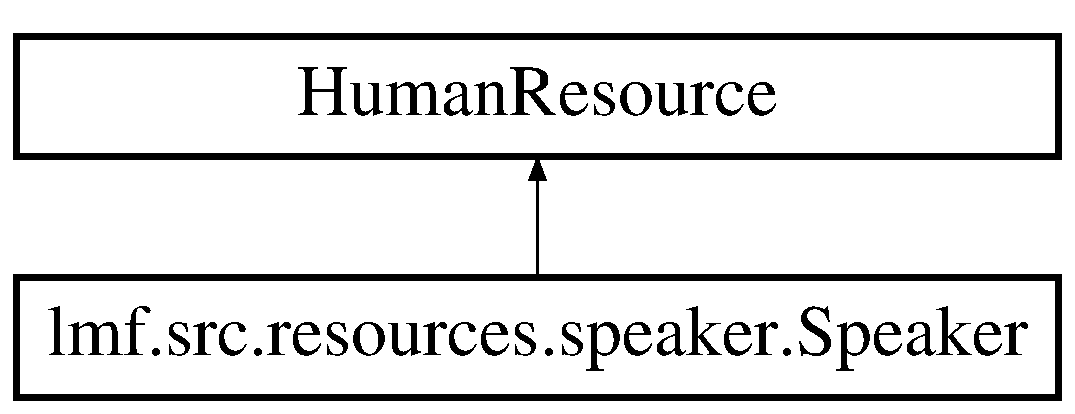
\includegraphics[height=2.000000cm]{classlmf_1_1src_1_1resources_1_1speaker_1_1_speaker}
\end{center}
\end{figure}
\subsection*{Public Member Functions}
\begin{DoxyCompactItemize}
\item 
def \hyperlink{classlmf_1_1src_1_1resources_1_1speaker_1_1_speaker_a73f8f0a5217cbef69ff7312842f70491}{\+\_\+\+\_\+init\+\_\+\+\_\+}
\begin{DoxyCompactList}\small\item\em Constructor. \end{DoxyCompactList}\item 
def \hyperlink{classlmf_1_1src_1_1resources_1_1speaker_1_1_speaker_a632d48e2ba734a90ad64b263f0f4e058}{\+\_\+\+\_\+del\+\_\+\+\_\+}
\begin{DoxyCompactList}\small\item\em Destructor. \end{DoxyCompactList}\end{DoxyCompactItemize}
\subsection*{Public Attributes}
\begin{DoxyCompactItemize}
\item 
\hyperlink{classlmf_1_1src_1_1resources_1_1speaker_1_1_speaker_a2773f1341512df6b9c9c5fb0f5c34cf5}{speaker\+I\+D}
\end{DoxyCompactItemize}


\subsection{Detailed Description}
\hyperlink{classlmf_1_1src_1_1resources_1_1speaker_1_1_speaker}{Speaker} is a Human\+Resource subclass. 

The \hyperlink{classlmf_1_1src_1_1resources_1_1speaker_1_1_speaker}{Speaker} is a class representing a speaker. 

Definition at line 8 of file speaker.\+py.



\subsection{Constructor \& Destructor Documentation}
\hypertarget{classlmf_1_1src_1_1resources_1_1speaker_1_1_speaker_a73f8f0a5217cbef69ff7312842f70491}{\index{lmf\+::src\+::resources\+::speaker\+::\+Speaker@{lmf\+::src\+::resources\+::speaker\+::\+Speaker}!\+\_\+\+\_\+init\+\_\+\+\_\+@{\+\_\+\+\_\+init\+\_\+\+\_\+}}
\index{\+\_\+\+\_\+init\+\_\+\+\_\+@{\+\_\+\+\_\+init\+\_\+\+\_\+}!lmf\+::src\+::resources\+::speaker\+::\+Speaker@{lmf\+::src\+::resources\+::speaker\+::\+Speaker}}
\subsubsection[{\+\_\+\+\_\+init\+\_\+\+\_\+}]{\setlength{\rightskip}{0pt plus 5cm}def lmf.\+src.\+resources.\+speaker.\+Speaker.\+\_\+\+\_\+init\+\_\+\+\_\+ (
\begin{DoxyParamCaption}
\item[{}]{self}
\end{DoxyParamCaption}
)}}\label{classlmf_1_1src_1_1resources_1_1speaker_1_1_speaker_a73f8f0a5217cbef69ff7312842f70491}


Constructor. 

\hyperlink{classlmf_1_1src_1_1resources_1_1speaker_1_1_speaker}{Speaker} instances are owned by Lexical\+Resource. \begin{DoxyReturn}{Returns}
A \hyperlink{classlmf_1_1src_1_1resources_1_1speaker_1_1_speaker}{Speaker} instance. 
\end{DoxyReturn}


Definition at line 11 of file speaker.\+py.

\hypertarget{classlmf_1_1src_1_1resources_1_1speaker_1_1_speaker_a632d48e2ba734a90ad64b263f0f4e058}{\index{lmf\+::src\+::resources\+::speaker\+::\+Speaker@{lmf\+::src\+::resources\+::speaker\+::\+Speaker}!\+\_\+\+\_\+del\+\_\+\+\_\+@{\+\_\+\+\_\+del\+\_\+\+\_\+}}
\index{\+\_\+\+\_\+del\+\_\+\+\_\+@{\+\_\+\+\_\+del\+\_\+\+\_\+}!lmf\+::src\+::resources\+::speaker\+::\+Speaker@{lmf\+::src\+::resources\+::speaker\+::\+Speaker}}
\subsubsection[{\+\_\+\+\_\+del\+\_\+\+\_\+}]{\setlength{\rightskip}{0pt plus 5cm}def lmf.\+src.\+resources.\+speaker.\+Speaker.\+\_\+\+\_\+del\+\_\+\+\_\+ (
\begin{DoxyParamCaption}
\item[{}]{self}
\end{DoxyParamCaption}
)}}\label{classlmf_1_1src_1_1resources_1_1speaker_1_1_speaker_a632d48e2ba734a90ad64b263f0f4e058}


Destructor. 



Definition at line 20 of file speaker.\+py.



\subsection{Member Data Documentation}
\hypertarget{classlmf_1_1src_1_1resources_1_1speaker_1_1_speaker_a2773f1341512df6b9c9c5fb0f5c34cf5}{\index{lmf\+::src\+::resources\+::speaker\+::\+Speaker@{lmf\+::src\+::resources\+::speaker\+::\+Speaker}!speaker\+I\+D@{speaker\+I\+D}}
\index{speaker\+I\+D@{speaker\+I\+D}!lmf\+::src\+::resources\+::speaker\+::\+Speaker@{lmf\+::src\+::resources\+::speaker\+::\+Speaker}}
\subsubsection[{speaker\+I\+D}]{\setlength{\rightskip}{0pt plus 5cm}lmf.\+src.\+resources.\+speaker.\+Speaker.\+speaker\+I\+D}}\label{classlmf_1_1src_1_1resources_1_1speaker_1_1_speaker_a2773f1341512df6b9c9c5fb0f5c34cf5}


Definition at line 18 of file speaker.\+py.



The documentation for this class was generated from the following file\+:\begin{DoxyCompactItemize}
\item 
/\+Users/celine/\+Work/\+C\+N\+R\+S/workspace/\+Himal\+Co/dev/lib/lmf/src/resources/\hyperlink{speaker_8py}{speaker.\+py}\end{DoxyCompactItemize}

\hypertarget{classlmf_1_1src_1_1core_1_1statement_1_1_statement}{\section{lmf.\+src.\+core.\+statement.\+Statement Class Reference}
\label{classlmf_1_1src_1_1core_1_1statement_1_1_statement}\index{lmf.\+src.\+core.\+statement.\+Statement@{lmf.\+src.\+core.\+statement.\+Statement}}
}


\char`\"{}\+Statement is a class representating a narrative description that refines or complements Definition.\char`\"{} (L\+M\+F)  


\subsection*{Public Member Functions}
\begin{DoxyCompactItemize}
\item 
def \hyperlink{classlmf_1_1src_1_1core_1_1statement_1_1_statement_ace7d3a3325c7f7b255a3dd72b20c74b1}{\+\_\+\+\_\+init\+\_\+\+\_\+}
\begin{DoxyCompactList}\small\item\em Constructor. \end{DoxyCompactList}\item 
def \hyperlink{classlmf_1_1src_1_1core_1_1statement_1_1_statement_a49d77869667dfde6c6abc794201f9fc3}{\+\_\+\+\_\+del\+\_\+\+\_\+}
\begin{DoxyCompactList}\small\item\em Destructor. \end{DoxyCompactList}\end{DoxyCompactItemize}
\subsection*{Public Attributes}
\begin{DoxyCompactItemize}
\item 
\hyperlink{classlmf_1_1src_1_1core_1_1statement_1_1_statement_abc61d06d03119e6e12d5c3854afc93c1}{note\+Type}
\item 
\hyperlink{classlmf_1_1src_1_1core_1_1statement_1_1_statement_a231fe52b0b7ba3deb6d0993987dddaf0}{note}
\item 
\hyperlink{classlmf_1_1src_1_1core_1_1statement_1_1_statement_a71a5b6eaf4bad349ab3399fbea06b88d}{language}
\item 
\hyperlink{classlmf_1_1src_1_1core_1_1statement_1_1_statement_a3f6a8d066930ce775d6f6655ea5f3dfa}{encyclopedic\+Information}
\item 
\hyperlink{classlmf_1_1src_1_1core_1_1statement_1_1_statement_a2e146c5f5de5eed52c082c2cc0bea7d0}{usage\+Note}
\item 
\hyperlink{classlmf_1_1src_1_1core_1_1statement_1_1_statement_a812bbd34658f5bfaf3babff001be9715}{restriction}
\item 
\hyperlink{classlmf_1_1src_1_1core_1_1statement_1_1_statement_afa73464513552afc8a6bf3828446a7d9}{derivation}
\item 
\hyperlink{classlmf_1_1src_1_1core_1_1statement_1_1_statement_a534b2190fdea34d7f085a78adaac1ee2}{borrowed\+Word}
\item 
\hyperlink{classlmf_1_1src_1_1core_1_1statement_1_1_statement_a4126cee37a75d852056ae49f45cf6cc3}{written\+Form}
\item 
\hyperlink{classlmf_1_1src_1_1core_1_1statement_1_1_statement_a1670c113f5b8143803936a3958d3f256}{sense}
\item 
\hyperlink{classlmf_1_1src_1_1core_1_1statement_1_1_statement_a1232c0098a52fa5f72d6a80c8661152a}{etymology}
\item 
\hyperlink{classlmf_1_1src_1_1core_1_1statement_1_1_statement_a25f9127cf2fe1017c53a3ccb57570352}{etymology\+Comment}
\item 
\hyperlink{classlmf_1_1src_1_1core_1_1statement_1_1_statement_a7d9d96cae746848b83b4ae8516c92bee}{etymology\+Gloss}
\item 
\hyperlink{classlmf_1_1src_1_1core_1_1statement_1_1_statement_adeefdc77c6ff898b8adba4ef2a946af3}{etymology\+Source}
\item 
\hyperlink{classlmf_1_1src_1_1core_1_1statement_1_1_statement_ac334fff77caf25a783e77aa55ca3128d}{term\+Source\+Language}
\item 
\hyperlink{classlmf_1_1src_1_1core_1_1statement_1_1_statement_aee57d23dce671062480f9b84ac43a2f1}{target\+Lexical\+Entry}
\item 
\hyperlink{classlmf_1_1src_1_1core_1_1statement_1_1_statement_a3af309c396e738565e75fff8df1b960a}{scientific\+Name}
\item 
\hyperlink{classlmf_1_1src_1_1core_1_1statement_1_1_statement_af2781856fbb02d55acc39864ec66aa24}{text\+\_\+representation}
\begin{DoxyCompactList}\small\item\em Text\+Representation instances are owned by \hyperlink{classlmf_1_1src_1_1core_1_1statement_1_1_statement}{Statement} There is zero to many Text\+Representation instances per \hyperlink{classlmf_1_1src_1_1core_1_1statement_1_1_statement}{Statement}. \end{DoxyCompactList}\end{DoxyCompactItemize}


\subsection{Detailed Description}
\char`\"{}\+Statement is a class representating a narrative description that refines or complements Definition.\char`\"{} (L\+M\+F) 

Definition at line 6 of file statement.\+py.



\subsection{Constructor \& Destructor Documentation}
\hypertarget{classlmf_1_1src_1_1core_1_1statement_1_1_statement_ace7d3a3325c7f7b255a3dd72b20c74b1}{\index{lmf\+::src\+::core\+::statement\+::\+Statement@{lmf\+::src\+::core\+::statement\+::\+Statement}!\+\_\+\+\_\+init\+\_\+\+\_\+@{\+\_\+\+\_\+init\+\_\+\+\_\+}}
\index{\+\_\+\+\_\+init\+\_\+\+\_\+@{\+\_\+\+\_\+init\+\_\+\+\_\+}!lmf\+::src\+::core\+::statement\+::\+Statement@{lmf\+::src\+::core\+::statement\+::\+Statement}}
\subsubsection[{\+\_\+\+\_\+init\+\_\+\+\_\+}]{\setlength{\rightskip}{0pt plus 5cm}def lmf.\+src.\+core.\+statement.\+Statement.\+\_\+\+\_\+init\+\_\+\+\_\+ (
\begin{DoxyParamCaption}
\item[{}]{self}
\end{DoxyParamCaption}
)}}\label{classlmf_1_1src_1_1core_1_1statement_1_1_statement_ace7d3a3325c7f7b255a3dd72b20c74b1}


Constructor. 

\hyperlink{classlmf_1_1src_1_1core_1_1statement_1_1_statement}{Statement} instances are owned by Definition. \begin{DoxyReturn}{Returns}
A \hyperlink{classlmf_1_1src_1_1core_1_1statement_1_1_statement}{Statement} instance. 
\end{DoxyReturn}


Definition at line 9 of file statement.\+py.

\hypertarget{classlmf_1_1src_1_1core_1_1statement_1_1_statement_a49d77869667dfde6c6abc794201f9fc3}{\index{lmf\+::src\+::core\+::statement\+::\+Statement@{lmf\+::src\+::core\+::statement\+::\+Statement}!\+\_\+\+\_\+del\+\_\+\+\_\+@{\+\_\+\+\_\+del\+\_\+\+\_\+}}
\index{\+\_\+\+\_\+del\+\_\+\+\_\+@{\+\_\+\+\_\+del\+\_\+\+\_\+}!lmf\+::src\+::core\+::statement\+::\+Statement@{lmf\+::src\+::core\+::statement\+::\+Statement}}
\subsubsection[{\+\_\+\+\_\+del\+\_\+\+\_\+}]{\setlength{\rightskip}{0pt plus 5cm}def lmf.\+src.\+core.\+statement.\+Statement.\+\_\+\+\_\+del\+\_\+\+\_\+ (
\begin{DoxyParamCaption}
\item[{}]{self}
\end{DoxyParamCaption}
)}}\label{classlmf_1_1src_1_1core_1_1statement_1_1_statement_a49d77869667dfde6c6abc794201f9fc3}


Destructor. 

Release Text\+Representation instances. 

Definition at line 35 of file statement.\+py.



\subsection{Member Data Documentation}
\hypertarget{classlmf_1_1src_1_1core_1_1statement_1_1_statement_a534b2190fdea34d7f085a78adaac1ee2}{\index{lmf\+::src\+::core\+::statement\+::\+Statement@{lmf\+::src\+::core\+::statement\+::\+Statement}!borrowed\+Word@{borrowed\+Word}}
\index{borrowed\+Word@{borrowed\+Word}!lmf\+::src\+::core\+::statement\+::\+Statement@{lmf\+::src\+::core\+::statement\+::\+Statement}}
\subsubsection[{borrowed\+Word}]{\setlength{\rightskip}{0pt plus 5cm}lmf.\+src.\+core.\+statement.\+Statement.\+borrowed\+Word}}\label{classlmf_1_1src_1_1core_1_1statement_1_1_statement_a534b2190fdea34d7f085a78adaac1ee2}


Definition at line 21 of file statement.\+py.

\hypertarget{classlmf_1_1src_1_1core_1_1statement_1_1_statement_afa73464513552afc8a6bf3828446a7d9}{\index{lmf\+::src\+::core\+::statement\+::\+Statement@{lmf\+::src\+::core\+::statement\+::\+Statement}!derivation@{derivation}}
\index{derivation@{derivation}!lmf\+::src\+::core\+::statement\+::\+Statement@{lmf\+::src\+::core\+::statement\+::\+Statement}}
\subsubsection[{derivation}]{\setlength{\rightskip}{0pt plus 5cm}lmf.\+src.\+core.\+statement.\+Statement.\+derivation}}\label{classlmf_1_1src_1_1core_1_1statement_1_1_statement_afa73464513552afc8a6bf3828446a7d9}


Definition at line 20 of file statement.\+py.

\hypertarget{classlmf_1_1src_1_1core_1_1statement_1_1_statement_a3f6a8d066930ce775d6f6655ea5f3dfa}{\index{lmf\+::src\+::core\+::statement\+::\+Statement@{lmf\+::src\+::core\+::statement\+::\+Statement}!encyclopedic\+Information@{encyclopedic\+Information}}
\index{encyclopedic\+Information@{encyclopedic\+Information}!lmf\+::src\+::core\+::statement\+::\+Statement@{lmf\+::src\+::core\+::statement\+::\+Statement}}
\subsubsection[{encyclopedic\+Information}]{\setlength{\rightskip}{0pt plus 5cm}lmf.\+src.\+core.\+statement.\+Statement.\+encyclopedic\+Information}}\label{classlmf_1_1src_1_1core_1_1statement_1_1_statement_a3f6a8d066930ce775d6f6655ea5f3dfa}


Definition at line 17 of file statement.\+py.

\hypertarget{classlmf_1_1src_1_1core_1_1statement_1_1_statement_a1232c0098a52fa5f72d6a80c8661152a}{\index{lmf\+::src\+::core\+::statement\+::\+Statement@{lmf\+::src\+::core\+::statement\+::\+Statement}!etymology@{etymology}}
\index{etymology@{etymology}!lmf\+::src\+::core\+::statement\+::\+Statement@{lmf\+::src\+::core\+::statement\+::\+Statement}}
\subsubsection[{etymology}]{\setlength{\rightskip}{0pt plus 5cm}lmf.\+src.\+core.\+statement.\+Statement.\+etymology}}\label{classlmf_1_1src_1_1core_1_1statement_1_1_statement_a1232c0098a52fa5f72d6a80c8661152a}


Definition at line 24 of file statement.\+py.

\hypertarget{classlmf_1_1src_1_1core_1_1statement_1_1_statement_a25f9127cf2fe1017c53a3ccb57570352}{\index{lmf\+::src\+::core\+::statement\+::\+Statement@{lmf\+::src\+::core\+::statement\+::\+Statement}!etymology\+Comment@{etymology\+Comment}}
\index{etymology\+Comment@{etymology\+Comment}!lmf\+::src\+::core\+::statement\+::\+Statement@{lmf\+::src\+::core\+::statement\+::\+Statement}}
\subsubsection[{etymology\+Comment}]{\setlength{\rightskip}{0pt plus 5cm}lmf.\+src.\+core.\+statement.\+Statement.\+etymology\+Comment}}\label{classlmf_1_1src_1_1core_1_1statement_1_1_statement_a25f9127cf2fe1017c53a3ccb57570352}


Definition at line 25 of file statement.\+py.

\hypertarget{classlmf_1_1src_1_1core_1_1statement_1_1_statement_a7d9d96cae746848b83b4ae8516c92bee}{\index{lmf\+::src\+::core\+::statement\+::\+Statement@{lmf\+::src\+::core\+::statement\+::\+Statement}!etymology\+Gloss@{etymology\+Gloss}}
\index{etymology\+Gloss@{etymology\+Gloss}!lmf\+::src\+::core\+::statement\+::\+Statement@{lmf\+::src\+::core\+::statement\+::\+Statement}}
\subsubsection[{etymology\+Gloss}]{\setlength{\rightskip}{0pt plus 5cm}lmf.\+src.\+core.\+statement.\+Statement.\+etymology\+Gloss}}\label{classlmf_1_1src_1_1core_1_1statement_1_1_statement_a7d9d96cae746848b83b4ae8516c92bee}


Definition at line 26 of file statement.\+py.

\hypertarget{classlmf_1_1src_1_1core_1_1statement_1_1_statement_adeefdc77c6ff898b8adba4ef2a946af3}{\index{lmf\+::src\+::core\+::statement\+::\+Statement@{lmf\+::src\+::core\+::statement\+::\+Statement}!etymology\+Source@{etymology\+Source}}
\index{etymology\+Source@{etymology\+Source}!lmf\+::src\+::core\+::statement\+::\+Statement@{lmf\+::src\+::core\+::statement\+::\+Statement}}
\subsubsection[{etymology\+Source}]{\setlength{\rightskip}{0pt plus 5cm}lmf.\+src.\+core.\+statement.\+Statement.\+etymology\+Source}}\label{classlmf_1_1src_1_1core_1_1statement_1_1_statement_adeefdc77c6ff898b8adba4ef2a946af3}


Definition at line 27 of file statement.\+py.

\hypertarget{classlmf_1_1src_1_1core_1_1statement_1_1_statement_a71a5b6eaf4bad349ab3399fbea06b88d}{\index{lmf\+::src\+::core\+::statement\+::\+Statement@{lmf\+::src\+::core\+::statement\+::\+Statement}!language@{language}}
\index{language@{language}!lmf\+::src\+::core\+::statement\+::\+Statement@{lmf\+::src\+::core\+::statement\+::\+Statement}}
\subsubsection[{language}]{\setlength{\rightskip}{0pt plus 5cm}lmf.\+src.\+core.\+statement.\+Statement.\+language}}\label{classlmf_1_1src_1_1core_1_1statement_1_1_statement_a71a5b6eaf4bad349ab3399fbea06b88d}


Definition at line 16 of file statement.\+py.

\hypertarget{classlmf_1_1src_1_1core_1_1statement_1_1_statement_a231fe52b0b7ba3deb6d0993987dddaf0}{\index{lmf\+::src\+::core\+::statement\+::\+Statement@{lmf\+::src\+::core\+::statement\+::\+Statement}!note@{note}}
\index{note@{note}!lmf\+::src\+::core\+::statement\+::\+Statement@{lmf\+::src\+::core\+::statement\+::\+Statement}}
\subsubsection[{note}]{\setlength{\rightskip}{0pt plus 5cm}lmf.\+src.\+core.\+statement.\+Statement.\+note}}\label{classlmf_1_1src_1_1core_1_1statement_1_1_statement_a231fe52b0b7ba3deb6d0993987dddaf0}


Definition at line 15 of file statement.\+py.

\hypertarget{classlmf_1_1src_1_1core_1_1statement_1_1_statement_abc61d06d03119e6e12d5c3854afc93c1}{\index{lmf\+::src\+::core\+::statement\+::\+Statement@{lmf\+::src\+::core\+::statement\+::\+Statement}!note\+Type@{note\+Type}}
\index{note\+Type@{note\+Type}!lmf\+::src\+::core\+::statement\+::\+Statement@{lmf\+::src\+::core\+::statement\+::\+Statement}}
\subsubsection[{note\+Type}]{\setlength{\rightskip}{0pt plus 5cm}lmf.\+src.\+core.\+statement.\+Statement.\+note\+Type}}\label{classlmf_1_1src_1_1core_1_1statement_1_1_statement_abc61d06d03119e6e12d5c3854afc93c1}


Definition at line 14 of file statement.\+py.

\hypertarget{classlmf_1_1src_1_1core_1_1statement_1_1_statement_a812bbd34658f5bfaf3babff001be9715}{\index{lmf\+::src\+::core\+::statement\+::\+Statement@{lmf\+::src\+::core\+::statement\+::\+Statement}!restriction@{restriction}}
\index{restriction@{restriction}!lmf\+::src\+::core\+::statement\+::\+Statement@{lmf\+::src\+::core\+::statement\+::\+Statement}}
\subsubsection[{restriction}]{\setlength{\rightskip}{0pt plus 5cm}lmf.\+src.\+core.\+statement.\+Statement.\+restriction}}\label{classlmf_1_1src_1_1core_1_1statement_1_1_statement_a812bbd34658f5bfaf3babff001be9715}


Definition at line 19 of file statement.\+py.

\hypertarget{classlmf_1_1src_1_1core_1_1statement_1_1_statement_a3af309c396e738565e75fff8df1b960a}{\index{lmf\+::src\+::core\+::statement\+::\+Statement@{lmf\+::src\+::core\+::statement\+::\+Statement}!scientific\+Name@{scientific\+Name}}
\index{scientific\+Name@{scientific\+Name}!lmf\+::src\+::core\+::statement\+::\+Statement@{lmf\+::src\+::core\+::statement\+::\+Statement}}
\subsubsection[{scientific\+Name}]{\setlength{\rightskip}{0pt plus 5cm}lmf.\+src.\+core.\+statement.\+Statement.\+scientific\+Name}}\label{classlmf_1_1src_1_1core_1_1statement_1_1_statement_a3af309c396e738565e75fff8df1b960a}


Definition at line 30 of file statement.\+py.

\hypertarget{classlmf_1_1src_1_1core_1_1statement_1_1_statement_a1670c113f5b8143803936a3958d3f256}{\index{lmf\+::src\+::core\+::statement\+::\+Statement@{lmf\+::src\+::core\+::statement\+::\+Statement}!sense@{sense}}
\index{sense@{sense}!lmf\+::src\+::core\+::statement\+::\+Statement@{lmf\+::src\+::core\+::statement\+::\+Statement}}
\subsubsection[{sense}]{\setlength{\rightskip}{0pt plus 5cm}lmf.\+src.\+core.\+statement.\+Statement.\+sense}}\label{classlmf_1_1src_1_1core_1_1statement_1_1_statement_a1670c113f5b8143803936a3958d3f256}


Definition at line 23 of file statement.\+py.

\hypertarget{classlmf_1_1src_1_1core_1_1statement_1_1_statement_aee57d23dce671062480f9b84ac43a2f1}{\index{lmf\+::src\+::core\+::statement\+::\+Statement@{lmf\+::src\+::core\+::statement\+::\+Statement}!target\+Lexical\+Entry@{target\+Lexical\+Entry}}
\index{target\+Lexical\+Entry@{target\+Lexical\+Entry}!lmf\+::src\+::core\+::statement\+::\+Statement@{lmf\+::src\+::core\+::statement\+::\+Statement}}
\subsubsection[{target\+Lexical\+Entry}]{\setlength{\rightskip}{0pt plus 5cm}lmf.\+src.\+core.\+statement.\+Statement.\+target\+Lexical\+Entry}}\label{classlmf_1_1src_1_1core_1_1statement_1_1_statement_aee57d23dce671062480f9b84ac43a2f1}


Definition at line 29 of file statement.\+py.

\hypertarget{classlmf_1_1src_1_1core_1_1statement_1_1_statement_ac334fff77caf25a783e77aa55ca3128d}{\index{lmf\+::src\+::core\+::statement\+::\+Statement@{lmf\+::src\+::core\+::statement\+::\+Statement}!term\+Source\+Language@{term\+Source\+Language}}
\index{term\+Source\+Language@{term\+Source\+Language}!lmf\+::src\+::core\+::statement\+::\+Statement@{lmf\+::src\+::core\+::statement\+::\+Statement}}
\subsubsection[{term\+Source\+Language}]{\setlength{\rightskip}{0pt plus 5cm}lmf.\+src.\+core.\+statement.\+Statement.\+term\+Source\+Language}}\label{classlmf_1_1src_1_1core_1_1statement_1_1_statement_ac334fff77caf25a783e77aa55ca3128d}


Definition at line 28 of file statement.\+py.

\hypertarget{classlmf_1_1src_1_1core_1_1statement_1_1_statement_af2781856fbb02d55acc39864ec66aa24}{\index{lmf\+::src\+::core\+::statement\+::\+Statement@{lmf\+::src\+::core\+::statement\+::\+Statement}!text\+\_\+representation@{text\+\_\+representation}}
\index{text\+\_\+representation@{text\+\_\+representation}!lmf\+::src\+::core\+::statement\+::\+Statement@{lmf\+::src\+::core\+::statement\+::\+Statement}}
\subsubsection[{text\+\_\+representation}]{\setlength{\rightskip}{0pt plus 5cm}lmf.\+src.\+core.\+statement.\+Statement.\+text\+\_\+representation}}\label{classlmf_1_1src_1_1core_1_1statement_1_1_statement_af2781856fbb02d55acc39864ec66aa24}


Text\+Representation instances are owned by \hyperlink{classlmf_1_1src_1_1core_1_1statement_1_1_statement}{Statement} There is zero to many Text\+Representation instances per \hyperlink{classlmf_1_1src_1_1core_1_1statement_1_1_statement}{Statement}. 



Definition at line 33 of file statement.\+py.

\hypertarget{classlmf_1_1src_1_1core_1_1statement_1_1_statement_a2e146c5f5de5eed52c082c2cc0bea7d0}{\index{lmf\+::src\+::core\+::statement\+::\+Statement@{lmf\+::src\+::core\+::statement\+::\+Statement}!usage\+Note@{usage\+Note}}
\index{usage\+Note@{usage\+Note}!lmf\+::src\+::core\+::statement\+::\+Statement@{lmf\+::src\+::core\+::statement\+::\+Statement}}
\subsubsection[{usage\+Note}]{\setlength{\rightskip}{0pt plus 5cm}lmf.\+src.\+core.\+statement.\+Statement.\+usage\+Note}}\label{classlmf_1_1src_1_1core_1_1statement_1_1_statement_a2e146c5f5de5eed52c082c2cc0bea7d0}


Definition at line 18 of file statement.\+py.

\hypertarget{classlmf_1_1src_1_1core_1_1statement_1_1_statement_a4126cee37a75d852056ae49f45cf6cc3}{\index{lmf\+::src\+::core\+::statement\+::\+Statement@{lmf\+::src\+::core\+::statement\+::\+Statement}!written\+Form@{written\+Form}}
\index{written\+Form@{written\+Form}!lmf\+::src\+::core\+::statement\+::\+Statement@{lmf\+::src\+::core\+::statement\+::\+Statement}}
\subsubsection[{written\+Form}]{\setlength{\rightskip}{0pt plus 5cm}lmf.\+src.\+core.\+statement.\+Statement.\+written\+Form}}\label{classlmf_1_1src_1_1core_1_1statement_1_1_statement_a4126cee37a75d852056ae49f45cf6cc3}


Definition at line 22 of file statement.\+py.



The documentation for this class was generated from the following file\+:\begin{DoxyCompactItemize}
\item 
/\+Users/celine/\+Work/\+C\+N\+R\+S/workspace/\+Himal\+Co/dev/lib/lmf/src/core/\hyperlink{statement_8py}{statement.\+py}\end{DoxyCompactItemize}

\hypertarget{classlmf_1_1src_1_1morphology_1_1stem_1_1_stem}{\section{lmf.\+src.\+morphology.\+stem.\+Stem Class Reference}
\label{classlmf_1_1src_1_1morphology_1_1stem_1_1_stem}\index{lmf.\+src.\+morphology.\+stem.\+Stem@{lmf.\+src.\+morphology.\+stem.\+Stem}}
}


\char`\"{}\+Stem is a Form subclass representing a morph, thus manages the sublexme parts\char`\"{} (L\+M\+F)  


Inheritance diagram for lmf.\+src.\+morphology.\+stem.\+Stem\+:\begin{figure}[H]
\begin{center}
\leavevmode
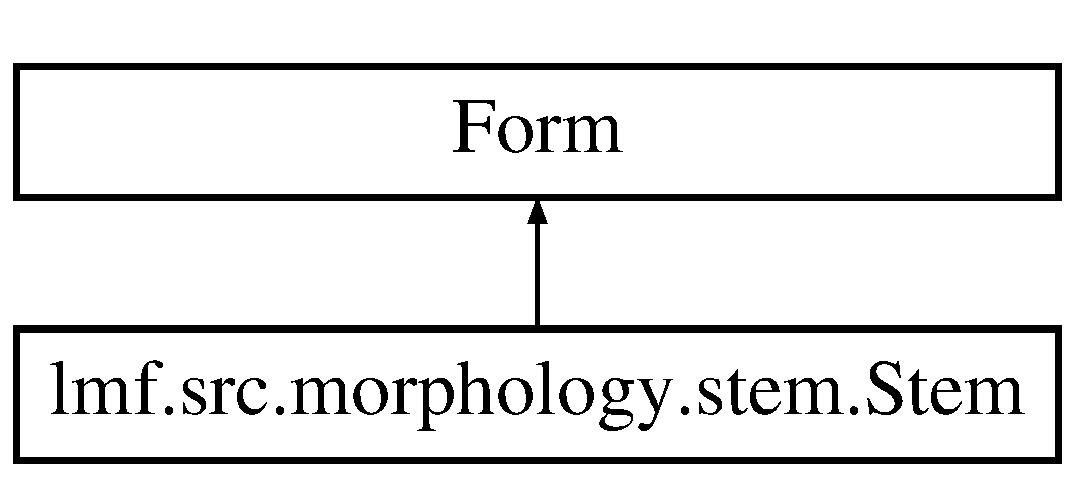
\includegraphics[height=2.000000cm]{classlmf_1_1src_1_1morphology_1_1stem_1_1_stem}
\end{center}
\end{figure}
\subsection*{Public Member Functions}
\begin{DoxyCompactItemize}
\item 
def \hyperlink{classlmf_1_1src_1_1morphology_1_1stem_1_1_stem_a0bb6ab66b2421c82cd8dffdd3bbc765d}{\+\_\+\+\_\+init\+\_\+\+\_\+}
\begin{DoxyCompactList}\small\item\em Constructor. \end{DoxyCompactList}\item 
def \hyperlink{classlmf_1_1src_1_1morphology_1_1stem_1_1_stem_a8081b50172bca2543d1a4989dbaf2f32}{\+\_\+\+\_\+del\+\_\+\+\_\+}
\begin{DoxyCompactList}\small\item\em Destructor. \end{DoxyCompactList}\end{DoxyCompactItemize}


\subsection{Detailed Description}
\char`\"{}\+Stem is a Form subclass representing a morph, thus manages the sublexme parts\char`\"{} (L\+M\+F) 

Definition at line 8 of file stem.\+py.



\subsection{Constructor \& Destructor Documentation}
\hypertarget{classlmf_1_1src_1_1morphology_1_1stem_1_1_stem_a0bb6ab66b2421c82cd8dffdd3bbc765d}{\index{lmf\+::src\+::morphology\+::stem\+::\+Stem@{lmf\+::src\+::morphology\+::stem\+::\+Stem}!\+\_\+\+\_\+init\+\_\+\+\_\+@{\+\_\+\+\_\+init\+\_\+\+\_\+}}
\index{\+\_\+\+\_\+init\+\_\+\+\_\+@{\+\_\+\+\_\+init\+\_\+\+\_\+}!lmf\+::src\+::morphology\+::stem\+::\+Stem@{lmf\+::src\+::morphology\+::stem\+::\+Stem}}
\subsubsection[{\+\_\+\+\_\+init\+\_\+\+\_\+}]{\setlength{\rightskip}{0pt plus 5cm}def lmf.\+src.\+morphology.\+stem.\+Stem.\+\_\+\+\_\+init\+\_\+\+\_\+ (
\begin{DoxyParamCaption}
\item[{}]{self}
\end{DoxyParamCaption}
)}}\label{classlmf_1_1src_1_1morphology_1_1stem_1_1_stem_a0bb6ab66b2421c82cd8dffdd3bbc765d}


Constructor. 

\hyperlink{classlmf_1_1src_1_1morphology_1_1stem_1_1_stem}{Stem} instances are owned by Lexical\+Entry. \begin{DoxyReturn}{Returns}
A \hyperlink{classlmf_1_1src_1_1morphology_1_1stem_1_1_stem}{Stem} instance. 
\end{DoxyReturn}


Definition at line 11 of file stem.\+py.

\hypertarget{classlmf_1_1src_1_1morphology_1_1stem_1_1_stem_a8081b50172bca2543d1a4989dbaf2f32}{\index{lmf\+::src\+::morphology\+::stem\+::\+Stem@{lmf\+::src\+::morphology\+::stem\+::\+Stem}!\+\_\+\+\_\+del\+\_\+\+\_\+@{\+\_\+\+\_\+del\+\_\+\+\_\+}}
\index{\+\_\+\+\_\+del\+\_\+\+\_\+@{\+\_\+\+\_\+del\+\_\+\+\_\+}!lmf\+::src\+::morphology\+::stem\+::\+Stem@{lmf\+::src\+::morphology\+::stem\+::\+Stem}}
\subsubsection[{\+\_\+\+\_\+del\+\_\+\+\_\+}]{\setlength{\rightskip}{0pt plus 5cm}def lmf.\+src.\+morphology.\+stem.\+Stem.\+\_\+\+\_\+del\+\_\+\+\_\+ (
\begin{DoxyParamCaption}
\item[{}]{self}
\end{DoxyParamCaption}
)}}\label{classlmf_1_1src_1_1morphology_1_1stem_1_1_stem_a8081b50172bca2543d1a4989dbaf2f32}


Destructor. 



Definition at line 19 of file stem.\+py.



The documentation for this class was generated from the following file\+:\begin{DoxyCompactItemize}
\item 
/\+Users/celine/\+Work/\+C\+N\+R\+S/workspace/\+Himal\+Co/dev/lib/lmf/src/morphology/\hyperlink{stem_8py}{stem.\+py}\end{DoxyCompactItemize}

\hypertarget{classlmf_1_1src_1_1mrd_1_1subject__field_1_1_subject_field}{\section{lmf.\+src.\+mrd.\+subject\+\_\+field.\+Subject\+Field Class Reference}
\label{classlmf_1_1src_1_1mrd_1_1subject__field_1_1_subject_field}\index{lmf.\+src.\+mrd.\+subject\+\_\+field.\+Subject\+Field@{lmf.\+src.\+mrd.\+subject\+\_\+field.\+Subject\+Field}}
}


\char`\"{}\+Subject Field is a class representing a text string that provides domain or status information.\char`\"{} (L\+M\+F)  


\subsection*{Public Member Functions}
\begin{DoxyCompactItemize}
\item 
def \hyperlink{classlmf_1_1src_1_1mrd_1_1subject__field_1_1_subject_field_a2d8f602d6bb1db753cac9f281c6ffc57}{\+\_\+\+\_\+init\+\_\+\+\_\+}
\begin{DoxyCompactList}\small\item\em Constructor. \end{DoxyCompactList}\item 
def \hyperlink{classlmf_1_1src_1_1mrd_1_1subject__field_1_1_subject_field_a15083c8ac78c8bd835dde95185af506e}{\+\_\+\+\_\+del\+\_\+\+\_\+}
\begin{DoxyCompactList}\small\item\em Destructor. \end{DoxyCompactList}\item 
def \hyperlink{classlmf_1_1src_1_1mrd_1_1subject__field_1_1_subject_field_ac4e9742f438398b1fa5037a93da6d311}{set\+\_\+semantic\+Domain}
\begin{DoxyCompactList}\small\item\em Set semantic domain and language. \end{DoxyCompactList}\item 
def \hyperlink{classlmf_1_1src_1_1mrd_1_1subject__field_1_1_subject_field_a3fc4634955416d9e363122adf4b48b16}{get\+\_\+semantic\+Domain}
\begin{DoxyCompactList}\small\item\em Get semantic domain. \end{DoxyCompactList}\item 
def \hyperlink{classlmf_1_1src_1_1mrd_1_1subject__field_1_1_subject_field_a7c83d664df89bcb5ee8fdda6a84b25fc}{set\+\_\+language}
\begin{DoxyCompactList}\small\item\em Set language used for semantic domain. \end{DoxyCompactList}\item 
def \hyperlink{classlmf_1_1src_1_1mrd_1_1subject__field_1_1_subject_field_ae74803856e84a12be44d438f957df0ca}{get\+\_\+language}
\begin{DoxyCompactList}\small\item\em Get language used for semantic domain. \end{DoxyCompactList}\item 
def \hyperlink{classlmf_1_1src_1_1mrd_1_1subject__field_1_1_subject_field_aaf00c3306172b2170a4038f0df9f3305}{create\+\_\+and\+\_\+add\+\_\+subject\+\_\+field}
\begin{DoxyCompactList}\small\item\em Create and add a subject field. \end{DoxyCompactList}\item 
def \hyperlink{classlmf_1_1src_1_1mrd_1_1subject__field_1_1_subject_field_ab291171fdd09053bf57f116da3516d14}{get\+\_\+subject\+\_\+fields}
\begin{DoxyCompactList}\small\item\em Get all subject fields maintained by this subject field. \end{DoxyCompactList}\item 
def \hyperlink{classlmf_1_1src_1_1mrd_1_1subject__field_1_1_subject_field_a1b9f4005c70ecde37f1946fe41eb2f4a}{set\+\_\+sub\+\_\+domain}
\begin{DoxyCompactList}\small\item\em Set a sub-\/domain and language. \end{DoxyCompactList}\item 
def \hyperlink{classlmf_1_1src_1_1mrd_1_1subject__field_1_1_subject_field_a8d5c74c0e79dedc43b428e724200a930}{get\+\_\+sub\+\_\+domains}
\begin{DoxyCompactList}\small\item\em Get all sub-\/domains. \end{DoxyCompactList}\end{DoxyCompactItemize}
\subsection*{Public Attributes}
\begin{DoxyCompactItemize}
\item 
\hyperlink{classlmf_1_1src_1_1mrd_1_1subject__field_1_1_subject_field_a32aad0bdc68774dbcc308df9bd73a00b}{language}
\item 
\hyperlink{classlmf_1_1src_1_1mrd_1_1subject__field_1_1_subject_field_aa625fa1b644690d878091eaa4ea9460f}{semantic\+Domain}
\item 
\hyperlink{classlmf_1_1src_1_1mrd_1_1subject__field_1_1_subject_field_ae43454d43d98b42b780661e8b18f89d4}{subject\+\_\+field}
\begin{DoxyCompactList}\small\item\em \hyperlink{classlmf_1_1src_1_1mrd_1_1subject__field_1_1_subject_field}{Subject\+Field} instances are owned by \hyperlink{classlmf_1_1src_1_1mrd_1_1subject__field_1_1_subject_field}{Subject\+Field} There is zero to many \hyperlink{classlmf_1_1src_1_1mrd_1_1subject__field_1_1_subject_field}{Subject\+Field} instances per \hyperlink{classlmf_1_1src_1_1mrd_1_1subject__field_1_1_subject_field}{Subject\+Field}. \end{DoxyCompactList}\end{DoxyCompactItemize}


\subsection{Detailed Description}
\char`\"{}\+Subject Field is a class representing a text string that provides domain or status information.\char`\"{} (L\+M\+F) 

Definition at line 8 of file subject\+\_\+field.\+py.



\subsection{Constructor \& Destructor Documentation}
\hypertarget{classlmf_1_1src_1_1mrd_1_1subject__field_1_1_subject_field_a2d8f602d6bb1db753cac9f281c6ffc57}{\index{lmf\+::src\+::mrd\+::subject\+\_\+field\+::\+Subject\+Field@{lmf\+::src\+::mrd\+::subject\+\_\+field\+::\+Subject\+Field}!\+\_\+\+\_\+init\+\_\+\+\_\+@{\+\_\+\+\_\+init\+\_\+\+\_\+}}
\index{\+\_\+\+\_\+init\+\_\+\+\_\+@{\+\_\+\+\_\+init\+\_\+\+\_\+}!lmf\+::src\+::mrd\+::subject\+\_\+field\+::\+Subject\+Field@{lmf\+::src\+::mrd\+::subject\+\_\+field\+::\+Subject\+Field}}
\subsubsection[{\+\_\+\+\_\+init\+\_\+\+\_\+}]{\setlength{\rightskip}{0pt plus 5cm}def lmf.\+src.\+mrd.\+subject\+\_\+field.\+Subject\+Field.\+\_\+\+\_\+init\+\_\+\+\_\+ (
\begin{DoxyParamCaption}
\item[{}]{self}
\end{DoxyParamCaption}
)}}\label{classlmf_1_1src_1_1mrd_1_1subject__field_1_1_subject_field_a2d8f602d6bb1db753cac9f281c6ffc57}


Constructor. 

\hyperlink{classlmf_1_1src_1_1mrd_1_1subject__field_1_1_subject_field}{Subject\+Field} instances are owned by Sense. \begin{DoxyReturn}{Returns}
A \hyperlink{classlmf_1_1src_1_1mrd_1_1subject__field_1_1_subject_field}{Subject\+Field} instance. 
\end{DoxyReturn}


Definition at line 11 of file subject\+\_\+field.\+py.

\hypertarget{classlmf_1_1src_1_1mrd_1_1subject__field_1_1_subject_field_a15083c8ac78c8bd835dde95185af506e}{\index{lmf\+::src\+::mrd\+::subject\+\_\+field\+::\+Subject\+Field@{lmf\+::src\+::mrd\+::subject\+\_\+field\+::\+Subject\+Field}!\+\_\+\+\_\+del\+\_\+\+\_\+@{\+\_\+\+\_\+del\+\_\+\+\_\+}}
\index{\+\_\+\+\_\+del\+\_\+\+\_\+@{\+\_\+\+\_\+del\+\_\+\+\_\+}!lmf\+::src\+::mrd\+::subject\+\_\+field\+::\+Subject\+Field@{lmf\+::src\+::mrd\+::subject\+\_\+field\+::\+Subject\+Field}}
\subsubsection[{\+\_\+\+\_\+del\+\_\+\+\_\+}]{\setlength{\rightskip}{0pt plus 5cm}def lmf.\+src.\+mrd.\+subject\+\_\+field.\+Subject\+Field.\+\_\+\+\_\+del\+\_\+\+\_\+ (
\begin{DoxyParamCaption}
\item[{}]{self}
\end{DoxyParamCaption}
)}}\label{classlmf_1_1src_1_1mrd_1_1subject__field_1_1_subject_field_a15083c8ac78c8bd835dde95185af506e}


Destructor. 

Release \hyperlink{classlmf_1_1src_1_1mrd_1_1subject__field_1_1_subject_field}{Subject\+Field} instances. 

Definition at line 22 of file subject\+\_\+field.\+py.



\subsection{Member Function Documentation}
\hypertarget{classlmf_1_1src_1_1mrd_1_1subject__field_1_1_subject_field_aaf00c3306172b2170a4038f0df9f3305}{\index{lmf\+::src\+::mrd\+::subject\+\_\+field\+::\+Subject\+Field@{lmf\+::src\+::mrd\+::subject\+\_\+field\+::\+Subject\+Field}!create\+\_\+and\+\_\+add\+\_\+subject\+\_\+field@{create\+\_\+and\+\_\+add\+\_\+subject\+\_\+field}}
\index{create\+\_\+and\+\_\+add\+\_\+subject\+\_\+field@{create\+\_\+and\+\_\+add\+\_\+subject\+\_\+field}!lmf\+::src\+::mrd\+::subject\+\_\+field\+::\+Subject\+Field@{lmf\+::src\+::mrd\+::subject\+\_\+field\+::\+Subject\+Field}}
\subsubsection[{create\+\_\+and\+\_\+add\+\_\+subject\+\_\+field}]{\setlength{\rightskip}{0pt plus 5cm}def lmf.\+src.\+mrd.\+subject\+\_\+field.\+Subject\+Field.\+create\+\_\+and\+\_\+add\+\_\+subject\+\_\+field (
\begin{DoxyParamCaption}
\item[{}]{self}
\end{DoxyParamCaption}
)}}\label{classlmf_1_1src_1_1mrd_1_1subject__field_1_1_subject_field_aaf00c3306172b2170a4038f0df9f3305}


Create and add a subject field. 

\begin{DoxyReturn}{Returns}
The created \hyperlink{classlmf_1_1src_1_1mrd_1_1subject__field_1_1_subject_field}{Subject\+Field} instance. 
\end{DoxyReturn}


Definition at line 67 of file subject\+\_\+field.\+py.

\hypertarget{classlmf_1_1src_1_1mrd_1_1subject__field_1_1_subject_field_ae74803856e84a12be44d438f957df0ca}{\index{lmf\+::src\+::mrd\+::subject\+\_\+field\+::\+Subject\+Field@{lmf\+::src\+::mrd\+::subject\+\_\+field\+::\+Subject\+Field}!get\+\_\+language@{get\+\_\+language}}
\index{get\+\_\+language@{get\+\_\+language}!lmf\+::src\+::mrd\+::subject\+\_\+field\+::\+Subject\+Field@{lmf\+::src\+::mrd\+::subject\+\_\+field\+::\+Subject\+Field}}
\subsubsection[{get\+\_\+language}]{\setlength{\rightskip}{0pt plus 5cm}def lmf.\+src.\+mrd.\+subject\+\_\+field.\+Subject\+Field.\+get\+\_\+language (
\begin{DoxyParamCaption}
\item[{}]{self}
\end{DoxyParamCaption}
)}}\label{classlmf_1_1src_1_1mrd_1_1subject__field_1_1_subject_field_ae74803856e84a12be44d438f957df0ca}


Get language used for semantic domain. 

\begin{DoxyReturn}{Returns}
\hyperlink{classlmf_1_1src_1_1mrd_1_1subject__field_1_1_subject_field}{Subject\+Field} attribute 'language'. 
\end{DoxyReturn}


Definition at line 61 of file subject\+\_\+field.\+py.

\hypertarget{classlmf_1_1src_1_1mrd_1_1subject__field_1_1_subject_field_a3fc4634955416d9e363122adf4b48b16}{\index{lmf\+::src\+::mrd\+::subject\+\_\+field\+::\+Subject\+Field@{lmf\+::src\+::mrd\+::subject\+\_\+field\+::\+Subject\+Field}!get\+\_\+semantic\+Domain@{get\+\_\+semantic\+Domain}}
\index{get\+\_\+semantic\+Domain@{get\+\_\+semantic\+Domain}!lmf\+::src\+::mrd\+::subject\+\_\+field\+::\+Subject\+Field@{lmf\+::src\+::mrd\+::subject\+\_\+field\+::\+Subject\+Field}}
\subsubsection[{get\+\_\+semantic\+Domain}]{\setlength{\rightskip}{0pt plus 5cm}def lmf.\+src.\+mrd.\+subject\+\_\+field.\+Subject\+Field.\+get\+\_\+semantic\+Domain (
\begin{DoxyParamCaption}
\item[{}]{self, }
\item[{}]{language = {\ttfamily None}}
\end{DoxyParamCaption}
)}}\label{classlmf_1_1src_1_1mrd_1_1subject__field_1_1_subject_field_a3fc4634955416d9e363122adf4b48b16}


Get semantic domain. 


\begin{DoxyParams}{Parameters}
{\em language} & If this argument is given, get semantic domain only if written in this language. \\
\hline
\end{DoxyParams}
\begin{DoxyReturn}{Returns}
The filtered \hyperlink{classlmf_1_1src_1_1mrd_1_1subject__field_1_1_subject_field}{Subject\+Field} attribute 'semantic\+Domain'. 
\end{DoxyReturn}


Definition at line 43 of file subject\+\_\+field.\+py.

\hypertarget{classlmf_1_1src_1_1mrd_1_1subject__field_1_1_subject_field_a8d5c74c0e79dedc43b428e724200a930}{\index{lmf\+::src\+::mrd\+::subject\+\_\+field\+::\+Subject\+Field@{lmf\+::src\+::mrd\+::subject\+\_\+field\+::\+Subject\+Field}!get\+\_\+sub\+\_\+domains@{get\+\_\+sub\+\_\+domains}}
\index{get\+\_\+sub\+\_\+domains@{get\+\_\+sub\+\_\+domains}!lmf\+::src\+::mrd\+::subject\+\_\+field\+::\+Subject\+Field@{lmf\+::src\+::mrd\+::subject\+\_\+field\+::\+Subject\+Field}}
\subsubsection[{get\+\_\+sub\+\_\+domains}]{\setlength{\rightskip}{0pt plus 5cm}def lmf.\+src.\+mrd.\+subject\+\_\+field.\+Subject\+Field.\+get\+\_\+sub\+\_\+domains (
\begin{DoxyParamCaption}
\item[{}]{self, }
\item[{}]{language = {\ttfamily None}}
\end{DoxyParamCaption}
)}}\label{classlmf_1_1src_1_1mrd_1_1subject__field_1_1_subject_field_a8d5c74c0e79dedc43b428e724200a930}


Get all sub-\/domains. 

Attribute 'semantic\+Domain' is owned by \hyperlink{classlmf_1_1src_1_1mrd_1_1subject__field_1_1_subject_field}{Subject\+Field}, which is owned by \hyperlink{classlmf_1_1src_1_1mrd_1_1subject__field_1_1_subject_field}{Subject\+Field}, etc. 
\begin{DoxyParams}{Parameters}
{\em language} & If this argument is given, get only semantic domains that are described using this language. \\
\hline
\end{DoxyParams}
\begin{DoxyReturn}{Returns}
A Python list of all \hyperlink{classlmf_1_1src_1_1mrd_1_1subject__field_1_1_subject_field}{Subject\+Field} attributes 'semantic\+Domain'. 
\end{DoxyReturn}


Definition at line 90 of file subject\+\_\+field.\+py.

\hypertarget{classlmf_1_1src_1_1mrd_1_1subject__field_1_1_subject_field_ab291171fdd09053bf57f116da3516d14}{\index{lmf\+::src\+::mrd\+::subject\+\_\+field\+::\+Subject\+Field@{lmf\+::src\+::mrd\+::subject\+\_\+field\+::\+Subject\+Field}!get\+\_\+subject\+\_\+fields@{get\+\_\+subject\+\_\+fields}}
\index{get\+\_\+subject\+\_\+fields@{get\+\_\+subject\+\_\+fields}!lmf\+::src\+::mrd\+::subject\+\_\+field\+::\+Subject\+Field@{lmf\+::src\+::mrd\+::subject\+\_\+field\+::\+Subject\+Field}}
\subsubsection[{get\+\_\+subject\+\_\+fields}]{\setlength{\rightskip}{0pt plus 5cm}def lmf.\+src.\+mrd.\+subject\+\_\+field.\+Subject\+Field.\+get\+\_\+subject\+\_\+fields (
\begin{DoxyParamCaption}
\item[{}]{self}
\end{DoxyParamCaption}
)}}\label{classlmf_1_1src_1_1mrd_1_1subject__field_1_1_subject_field_ab291171fdd09053bf57f116da3516d14}


Get all subject fields maintained by this subject field. 

\begin{DoxyReturn}{Returns}
A Python list of subject fields. 
\end{DoxyReturn}


Definition at line 75 of file subject\+\_\+field.\+py.

\hypertarget{classlmf_1_1src_1_1mrd_1_1subject__field_1_1_subject_field_a7c83d664df89bcb5ee8fdda6a84b25fc}{\index{lmf\+::src\+::mrd\+::subject\+\_\+field\+::\+Subject\+Field@{lmf\+::src\+::mrd\+::subject\+\_\+field\+::\+Subject\+Field}!set\+\_\+language@{set\+\_\+language}}
\index{set\+\_\+language@{set\+\_\+language}!lmf\+::src\+::mrd\+::subject\+\_\+field\+::\+Subject\+Field@{lmf\+::src\+::mrd\+::subject\+\_\+field\+::\+Subject\+Field}}
\subsubsection[{set\+\_\+language}]{\setlength{\rightskip}{0pt plus 5cm}def lmf.\+src.\+mrd.\+subject\+\_\+field.\+Subject\+Field.\+set\+\_\+language (
\begin{DoxyParamCaption}
\item[{}]{self, }
\item[{}]{language}
\end{DoxyParamCaption}
)}}\label{classlmf_1_1src_1_1mrd_1_1subject__field_1_1_subject_field_a7c83d664df89bcb5ee8fdda6a84b25fc}


Set language used for semantic domain. 


\begin{DoxyParams}{Parameters}
{\em language} & Language used to describe the semantic domain. \\
\hline
\end{DoxyParams}
\begin{DoxyReturn}{Returns}
\hyperlink{classlmf_1_1src_1_1mrd_1_1subject__field_1_1_subject_field}{Subject\+Field} instance. 
\end{DoxyReturn}


Definition at line 51 of file subject\+\_\+field.\+py.

\hypertarget{classlmf_1_1src_1_1mrd_1_1subject__field_1_1_subject_field_ac4e9742f438398b1fa5037a93da6d311}{\index{lmf\+::src\+::mrd\+::subject\+\_\+field\+::\+Subject\+Field@{lmf\+::src\+::mrd\+::subject\+\_\+field\+::\+Subject\+Field}!set\+\_\+semantic\+Domain@{set\+\_\+semantic\+Domain}}
\index{set\+\_\+semantic\+Domain@{set\+\_\+semantic\+Domain}!lmf\+::src\+::mrd\+::subject\+\_\+field\+::\+Subject\+Field@{lmf\+::src\+::mrd\+::subject\+\_\+field\+::\+Subject\+Field}}
\subsubsection[{set\+\_\+semantic\+Domain}]{\setlength{\rightskip}{0pt plus 5cm}def lmf.\+src.\+mrd.\+subject\+\_\+field.\+Subject\+Field.\+set\+\_\+semantic\+Domain (
\begin{DoxyParamCaption}
\item[{}]{self, }
\item[{}]{semantic\+\_\+domain, }
\item[{}]{language = {\ttfamily None}}
\end{DoxyParamCaption}
)}}\label{classlmf_1_1src_1_1mrd_1_1subject__field_1_1_subject_field_ac4e9742f438398b1fa5037a93da6d311}


Set semantic domain and language. 


\begin{DoxyParams}{Parameters}
{\em semantic\+\_\+domain} & The semantic domain to set. \\
\hline
{\em language} & Language used to describe the semantic domain. \\
\hline
\end{DoxyParams}
\begin{DoxyReturn}{Returns}
\hyperlink{classlmf_1_1src_1_1mrd_1_1subject__field_1_1_subject_field}{Subject\+Field} instance. 
\end{DoxyReturn}


Definition at line 30 of file subject\+\_\+field.\+py.

\hypertarget{classlmf_1_1src_1_1mrd_1_1subject__field_1_1_subject_field_a1b9f4005c70ecde37f1946fe41eb2f4a}{\index{lmf\+::src\+::mrd\+::subject\+\_\+field\+::\+Subject\+Field@{lmf\+::src\+::mrd\+::subject\+\_\+field\+::\+Subject\+Field}!set\+\_\+sub\+\_\+domain@{set\+\_\+sub\+\_\+domain}}
\index{set\+\_\+sub\+\_\+domain@{set\+\_\+sub\+\_\+domain}!lmf\+::src\+::mrd\+::subject\+\_\+field\+::\+Subject\+Field@{lmf\+::src\+::mrd\+::subject\+\_\+field\+::\+Subject\+Field}}
\subsubsection[{set\+\_\+sub\+\_\+domain}]{\setlength{\rightskip}{0pt plus 5cm}def lmf.\+src.\+mrd.\+subject\+\_\+field.\+Subject\+Field.\+set\+\_\+sub\+\_\+domain (
\begin{DoxyParamCaption}
\item[{}]{self, }
\item[{}]{semantic\+\_\+domain, }
\item[{}]{language = {\ttfamily None}}
\end{DoxyParamCaption}
)}}\label{classlmf_1_1src_1_1mrd_1_1subject__field_1_1_subject_field_a1b9f4005c70ecde37f1946fe41eb2f4a}


Set a sub-\/domain and language. 


\begin{DoxyParams}{Parameters}
{\em semantic\+\_\+domain} & The sub-\/domain to set. \\
\hline
{\em language} & Language used to describe the sub-\/domain. \\
\hline
\end{DoxyParams}
\begin{DoxyReturn}{Returns}
\hyperlink{classlmf_1_1src_1_1mrd_1_1subject__field_1_1_subject_field}{Subject\+Field} instance. 
\end{DoxyReturn}


Definition at line 81 of file subject\+\_\+field.\+py.



\subsection{Member Data Documentation}
\hypertarget{classlmf_1_1src_1_1mrd_1_1subject__field_1_1_subject_field_a32aad0bdc68774dbcc308df9bd73a00b}{\index{lmf\+::src\+::mrd\+::subject\+\_\+field\+::\+Subject\+Field@{lmf\+::src\+::mrd\+::subject\+\_\+field\+::\+Subject\+Field}!language@{language}}
\index{language@{language}!lmf\+::src\+::mrd\+::subject\+\_\+field\+::\+Subject\+Field@{lmf\+::src\+::mrd\+::subject\+\_\+field\+::\+Subject\+Field}}
\subsubsection[{language}]{\setlength{\rightskip}{0pt plus 5cm}lmf.\+src.\+mrd.\+subject\+\_\+field.\+Subject\+Field.\+language}}\label{classlmf_1_1src_1_1mrd_1_1subject__field_1_1_subject_field_a32aad0bdc68774dbcc308df9bd73a00b}


Definition at line 16 of file subject\+\_\+field.\+py.

\hypertarget{classlmf_1_1src_1_1mrd_1_1subject__field_1_1_subject_field_aa625fa1b644690d878091eaa4ea9460f}{\index{lmf\+::src\+::mrd\+::subject\+\_\+field\+::\+Subject\+Field@{lmf\+::src\+::mrd\+::subject\+\_\+field\+::\+Subject\+Field}!semantic\+Domain@{semantic\+Domain}}
\index{semantic\+Domain@{semantic\+Domain}!lmf\+::src\+::mrd\+::subject\+\_\+field\+::\+Subject\+Field@{lmf\+::src\+::mrd\+::subject\+\_\+field\+::\+Subject\+Field}}
\subsubsection[{semantic\+Domain}]{\setlength{\rightskip}{0pt plus 5cm}lmf.\+src.\+mrd.\+subject\+\_\+field.\+Subject\+Field.\+semantic\+Domain}}\label{classlmf_1_1src_1_1mrd_1_1subject__field_1_1_subject_field_aa625fa1b644690d878091eaa4ea9460f}


Definition at line 17 of file subject\+\_\+field.\+py.

\hypertarget{classlmf_1_1src_1_1mrd_1_1subject__field_1_1_subject_field_ae43454d43d98b42b780661e8b18f89d4}{\index{lmf\+::src\+::mrd\+::subject\+\_\+field\+::\+Subject\+Field@{lmf\+::src\+::mrd\+::subject\+\_\+field\+::\+Subject\+Field}!subject\+\_\+field@{subject\+\_\+field}}
\index{subject\+\_\+field@{subject\+\_\+field}!lmf\+::src\+::mrd\+::subject\+\_\+field\+::\+Subject\+Field@{lmf\+::src\+::mrd\+::subject\+\_\+field\+::\+Subject\+Field}}
\subsubsection[{subject\+\_\+field}]{\setlength{\rightskip}{0pt plus 5cm}lmf.\+src.\+mrd.\+subject\+\_\+field.\+Subject\+Field.\+subject\+\_\+field}}\label{classlmf_1_1src_1_1mrd_1_1subject__field_1_1_subject_field_ae43454d43d98b42b780661e8b18f89d4}


\hyperlink{classlmf_1_1src_1_1mrd_1_1subject__field_1_1_subject_field}{Subject\+Field} instances are owned by \hyperlink{classlmf_1_1src_1_1mrd_1_1subject__field_1_1_subject_field}{Subject\+Field} There is zero to many \hyperlink{classlmf_1_1src_1_1mrd_1_1subject__field_1_1_subject_field}{Subject\+Field} instances per \hyperlink{classlmf_1_1src_1_1mrd_1_1subject__field_1_1_subject_field}{Subject\+Field}. 



Definition at line 20 of file subject\+\_\+field.\+py.



The documentation for this class was generated from the following file\+:\begin{DoxyCompactItemize}
\item 
/\+Users/celine/\+Work/\+C\+N\+R\+S/workspace/\+Himal\+Co/dev/lib/lmf/src/mrd/\hyperlink{subject__field_8py}{subject\+\_\+field.\+py}\end{DoxyCompactItemize}

\hypertarget{classlmf_1_1src_1_1core_1_1text__representation_1_1_text_representation}{\section{lmf.\+src.\+core.\+text\+\_\+representation.\+Text\+Representation Class Reference}
\label{classlmf_1_1src_1_1core_1_1text__representation_1_1_text_representation}\index{lmf.\+src.\+core.\+text\+\_\+representation.\+Text\+Representation@{lmf.\+src.\+core.\+text\+\_\+representation.\+Text\+Representation}}
}


\char`\"{}\+Text Representation is a class representing the textual content of definition or statement. When there is more than one variant orthography, the Text Representation instance contains a Unicode string representing the textual content as well as unique attribute-\/value pairs that describe the specific language, script and orthography.\char`\"{} (L\+M\+F)  


Inheritance diagram for lmf.\+src.\+core.\+text\+\_\+representation.\+Text\+Representation\+:\begin{figure}[H]
\begin{center}
\leavevmode
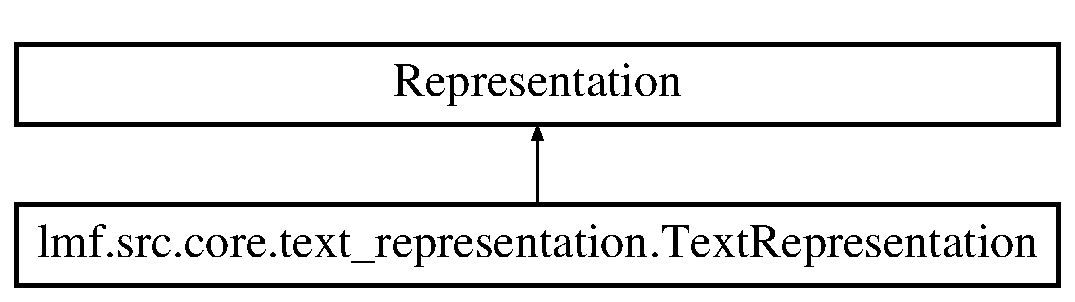
\includegraphics[height=2.000000cm]{classlmf_1_1src_1_1core_1_1text__representation_1_1_text_representation}
\end{center}
\end{figure}
\subsection*{Public Member Functions}
\begin{DoxyCompactItemize}
\item 
def \hyperlink{classlmf_1_1src_1_1core_1_1text__representation_1_1_text_representation_a44896bbde1027d1156df6f3c6396a117}{\+\_\+\+\_\+init\+\_\+\+\_\+}
\begin{DoxyCompactList}\small\item\em Constructor. \end{DoxyCompactList}\item 
def \hyperlink{classlmf_1_1src_1_1core_1_1text__representation_1_1_text_representation_aca36ddfaa299552d8248fd6ce08202a1}{\+\_\+\+\_\+del\+\_\+\+\_\+}
\begin{DoxyCompactList}\small\item\em Destructor. \end{DoxyCompactList}\item 
def \hyperlink{classlmf_1_1src_1_1core_1_1text__representation_1_1_text_representation_a84a6b65581f2e327a47989912c33838a}{set\+\_\+comment}
\begin{DoxyCompactList}\small\item\em Set written form comment. \end{DoxyCompactList}\item 
def \hyperlink{classlmf_1_1src_1_1core_1_1text__representation_1_1_text_representation_a3211a3da3b34f68aa4d6542aafe940ee}{get\+\_\+comment}
\begin{DoxyCompactList}\small\item\em Get written form comment. \end{DoxyCompactList}\item 
def \hyperlink{classlmf_1_1src_1_1core_1_1text__representation_1_1_text_representation_a6ecc8173f69656c0135368ded971ceea}{set\+\_\+written\+Form}
\begin{DoxyCompactList}\small\item\em Set written form and language. \end{DoxyCompactList}\item 
def \hyperlink{classlmf_1_1src_1_1core_1_1text__representation_1_1_text_representation_a85adf686ca1d5df10588f312260390e9}{get\+\_\+written\+Form}
\begin{DoxyCompactList}\small\item\em Get written form. \end{DoxyCompactList}\item 
def \hyperlink{classlmf_1_1src_1_1core_1_1text__representation_1_1_text_representation_a00be4c8e0a058f9df2605abb27ac8853}{set\+\_\+language}
\begin{DoxyCompactList}\small\item\em Set language used for written form. \end{DoxyCompactList}\item 
def \hyperlink{classlmf_1_1src_1_1core_1_1text__representation_1_1_text_representation_a1ec2b944809b0503bc1bb07b034eef5b}{get\+\_\+language}
\begin{DoxyCompactList}\small\item\em Get language used for written form. \end{DoxyCompactList}\item 
def \hyperlink{classlmf_1_1src_1_1core_1_1text__representation_1_1_text_representation_ae7d072249f81b508e86b086fd80f27a7}{set\+\_\+script\+Name}
\begin{DoxyCompactList}\small\item\em Set script name. \end{DoxyCompactList}\item 
def \hyperlink{classlmf_1_1src_1_1core_1_1text__representation_1_1_text_representation_aba63d43929e12252bc2ac535b6d3f563}{get\+\_\+script\+Name}
\begin{DoxyCompactList}\small\item\em Get script name. \end{DoxyCompactList}\end{DoxyCompactItemize}
\subsection*{Public Attributes}
\begin{DoxyCompactItemize}
\item 
\hyperlink{classlmf_1_1src_1_1core_1_1text__representation_1_1_text_representation_a78df11b119c24be8b18e6f121e0bb802}{font}
\item 
\hyperlink{classlmf_1_1src_1_1core_1_1text__representation_1_1_text_representation_af0026ed9d19dd869b408fba84f6fa5b1}{comment}
\item 
\hyperlink{classlmf_1_1src_1_1core_1_1text__representation_1_1_text_representation_a029a488706154d5fe42ecbea00974780}{written\+Form}
\item 
\hyperlink{classlmf_1_1src_1_1core_1_1text__representation_1_1_text_representation_aba23f79743bc4aa642f344aec09a3807}{language}
\item 
\hyperlink{classlmf_1_1src_1_1core_1_1text__representation_1_1_text_representation_a1aeda3c7310f02affa313c8797bfaf65}{script\+Name}
\end{DoxyCompactItemize}


\subsection{Detailed Description}
\char`\"{}\+Text Representation is a class representing the textual content of definition or statement. When there is more than one variant orthography, the Text Representation instance contains a Unicode string representing the textual content as well as unique attribute-\/value pairs that describe the specific language, script and orthography.\char`\"{} (L\+M\+F) 

Definition at line 9 of file text\+\_\+representation.\+py.



\subsection{Constructor \& Destructor Documentation}
\hypertarget{classlmf_1_1src_1_1core_1_1text__representation_1_1_text_representation_a44896bbde1027d1156df6f3c6396a117}{\index{lmf\+::src\+::core\+::text\+\_\+representation\+::\+Text\+Representation@{lmf\+::src\+::core\+::text\+\_\+representation\+::\+Text\+Representation}!\+\_\+\+\_\+init\+\_\+\+\_\+@{\+\_\+\+\_\+init\+\_\+\+\_\+}}
\index{\+\_\+\+\_\+init\+\_\+\+\_\+@{\+\_\+\+\_\+init\+\_\+\+\_\+}!lmf\+::src\+::core\+::text\+\_\+representation\+::\+Text\+Representation@{lmf\+::src\+::core\+::text\+\_\+representation\+::\+Text\+Representation}}
\subsubsection[{\+\_\+\+\_\+init\+\_\+\+\_\+}]{\setlength{\rightskip}{0pt plus 5cm}def lmf.\+src.\+core.\+text\+\_\+representation.\+Text\+Representation.\+\_\+\+\_\+init\+\_\+\+\_\+ (
\begin{DoxyParamCaption}
\item[{}]{self}
\end{DoxyParamCaption}
)}}\label{classlmf_1_1src_1_1core_1_1text__representation_1_1_text_representation_a44896bbde1027d1156df6f3c6396a117}


Constructor. 

\hyperlink{classlmf_1_1src_1_1core_1_1text__representation_1_1_text_representation}{Text\+Representation} instances are owned by Definition and Statement. \begin{DoxyReturn}{Returns}
A \hyperlink{classlmf_1_1src_1_1core_1_1text__representation_1_1_text_representation}{Text\+Representation} instance. 
\end{DoxyReturn}


Definition at line 12 of file text\+\_\+representation.\+py.

\hypertarget{classlmf_1_1src_1_1core_1_1text__representation_1_1_text_representation_aca36ddfaa299552d8248fd6ce08202a1}{\index{lmf\+::src\+::core\+::text\+\_\+representation\+::\+Text\+Representation@{lmf\+::src\+::core\+::text\+\_\+representation\+::\+Text\+Representation}!\+\_\+\+\_\+del\+\_\+\+\_\+@{\+\_\+\+\_\+del\+\_\+\+\_\+}}
\index{\+\_\+\+\_\+del\+\_\+\+\_\+@{\+\_\+\+\_\+del\+\_\+\+\_\+}!lmf\+::src\+::core\+::text\+\_\+representation\+::\+Text\+Representation@{lmf\+::src\+::core\+::text\+\_\+representation\+::\+Text\+Representation}}
\subsubsection[{\+\_\+\+\_\+del\+\_\+\+\_\+}]{\setlength{\rightskip}{0pt plus 5cm}def lmf.\+src.\+core.\+text\+\_\+representation.\+Text\+Representation.\+\_\+\+\_\+del\+\_\+\+\_\+ (
\begin{DoxyParamCaption}
\item[{}]{self}
\end{DoxyParamCaption}
)}}\label{classlmf_1_1src_1_1core_1_1text__representation_1_1_text_representation_aca36ddfaa299552d8248fd6ce08202a1}


Destructor. 



Definition at line 21 of file text\+\_\+representation.\+py.



\subsection{Member Function Documentation}
\hypertarget{classlmf_1_1src_1_1core_1_1text__representation_1_1_text_representation_a3211a3da3b34f68aa4d6542aafe940ee}{\index{lmf\+::src\+::core\+::text\+\_\+representation\+::\+Text\+Representation@{lmf\+::src\+::core\+::text\+\_\+representation\+::\+Text\+Representation}!get\+\_\+comment@{get\+\_\+comment}}
\index{get\+\_\+comment@{get\+\_\+comment}!lmf\+::src\+::core\+::text\+\_\+representation\+::\+Text\+Representation@{lmf\+::src\+::core\+::text\+\_\+representation\+::\+Text\+Representation}}
\subsubsection[{get\+\_\+comment}]{\setlength{\rightskip}{0pt plus 5cm}def lmf.\+src.\+core.\+text\+\_\+representation.\+Text\+Representation.\+get\+\_\+comment (
\begin{DoxyParamCaption}
\item[{}]{self}
\end{DoxyParamCaption}
)}}\label{classlmf_1_1src_1_1core_1_1text__representation_1_1_text_representation_a3211a3da3b34f68aa4d6542aafe940ee}


Get written form comment. 

\begin{DoxyReturn}{Returns}
Representation attribute 'comment'. 
\end{DoxyReturn}


Definition at line 36 of file text\+\_\+representation.\+py.

\hypertarget{classlmf_1_1src_1_1core_1_1text__representation_1_1_text_representation_a1ec2b944809b0503bc1bb07b034eef5b}{\index{lmf\+::src\+::core\+::text\+\_\+representation\+::\+Text\+Representation@{lmf\+::src\+::core\+::text\+\_\+representation\+::\+Text\+Representation}!get\+\_\+language@{get\+\_\+language}}
\index{get\+\_\+language@{get\+\_\+language}!lmf\+::src\+::core\+::text\+\_\+representation\+::\+Text\+Representation@{lmf\+::src\+::core\+::text\+\_\+representation\+::\+Text\+Representation}}
\subsubsection[{get\+\_\+language}]{\setlength{\rightskip}{0pt plus 5cm}def lmf.\+src.\+core.\+text\+\_\+representation.\+Text\+Representation.\+get\+\_\+language (
\begin{DoxyParamCaption}
\item[{}]{self}
\end{DoxyParamCaption}
)}}\label{classlmf_1_1src_1_1core_1_1text__representation_1_1_text_representation_a1ec2b944809b0503bc1bb07b034eef5b}


Get language used for written form. 

\begin{DoxyReturn}{Returns}
Representation attribute 'language'. 
\end{DoxyReturn}


Definition at line 73 of file text\+\_\+representation.\+py.

\hypertarget{classlmf_1_1src_1_1core_1_1text__representation_1_1_text_representation_aba63d43929e12252bc2ac535b6d3f563}{\index{lmf\+::src\+::core\+::text\+\_\+representation\+::\+Text\+Representation@{lmf\+::src\+::core\+::text\+\_\+representation\+::\+Text\+Representation}!get\+\_\+script\+Name@{get\+\_\+script\+Name}}
\index{get\+\_\+script\+Name@{get\+\_\+script\+Name}!lmf\+::src\+::core\+::text\+\_\+representation\+::\+Text\+Representation@{lmf\+::src\+::core\+::text\+\_\+representation\+::\+Text\+Representation}}
\subsubsection[{get\+\_\+script\+Name}]{\setlength{\rightskip}{0pt plus 5cm}def lmf.\+src.\+core.\+text\+\_\+representation.\+Text\+Representation.\+get\+\_\+script\+Name (
\begin{DoxyParamCaption}
\item[{}]{self}
\end{DoxyParamCaption}
)}}\label{classlmf_1_1src_1_1core_1_1text__representation_1_1_text_representation_aba63d43929e12252bc2ac535b6d3f563}


Get script name. 

\begin{DoxyReturn}{Returns}
Representation attribute 'script\+Name'. 
\end{DoxyReturn}


Definition at line 89 of file text\+\_\+representation.\+py.

\hypertarget{classlmf_1_1src_1_1core_1_1text__representation_1_1_text_representation_a85adf686ca1d5df10588f312260390e9}{\index{lmf\+::src\+::core\+::text\+\_\+representation\+::\+Text\+Representation@{lmf\+::src\+::core\+::text\+\_\+representation\+::\+Text\+Representation}!get\+\_\+written\+Form@{get\+\_\+written\+Form}}
\index{get\+\_\+written\+Form@{get\+\_\+written\+Form}!lmf\+::src\+::core\+::text\+\_\+representation\+::\+Text\+Representation@{lmf\+::src\+::core\+::text\+\_\+representation\+::\+Text\+Representation}}
\subsubsection[{get\+\_\+written\+Form}]{\setlength{\rightskip}{0pt plus 5cm}def lmf.\+src.\+core.\+text\+\_\+representation.\+Text\+Representation.\+get\+\_\+written\+Form (
\begin{DoxyParamCaption}
\item[{}]{self, }
\item[{}]{language = {\ttfamily None}}
\end{DoxyParamCaption}
)}}\label{classlmf_1_1src_1_1core_1_1text__representation_1_1_text_representation_a85adf686ca1d5df10588f312260390e9}


Get written form. 


\begin{DoxyParams}{Parameters}
{\em language} & If this argument is given, get written form only if written in this language. \\
\hline
\end{DoxyParams}
\begin{DoxyReturn}{Returns}
The filtered Representation attribute 'written\+Form'. 
\end{DoxyReturn}


Definition at line 55 of file text\+\_\+representation.\+py.

\hypertarget{classlmf_1_1src_1_1core_1_1text__representation_1_1_text_representation_a84a6b65581f2e327a47989912c33838a}{\index{lmf\+::src\+::core\+::text\+\_\+representation\+::\+Text\+Representation@{lmf\+::src\+::core\+::text\+\_\+representation\+::\+Text\+Representation}!set\+\_\+comment@{set\+\_\+comment}}
\index{set\+\_\+comment@{set\+\_\+comment}!lmf\+::src\+::core\+::text\+\_\+representation\+::\+Text\+Representation@{lmf\+::src\+::core\+::text\+\_\+representation\+::\+Text\+Representation}}
\subsubsection[{set\+\_\+comment}]{\setlength{\rightskip}{0pt plus 5cm}def lmf.\+src.\+core.\+text\+\_\+representation.\+Text\+Representation.\+set\+\_\+comment (
\begin{DoxyParamCaption}
\item[{}]{self, }
\item[{}]{comment}
\end{DoxyParamCaption}
)}}\label{classlmf_1_1src_1_1core_1_1text__representation_1_1_text_representation_a84a6b65581f2e327a47989912c33838a}


Set written form comment. 


\begin{DoxyParams}{Parameters}
{\em comment} & Comment about the written form. \\
\hline
\end{DoxyParams}
\begin{DoxyReturn}{Returns}
\hyperlink{classlmf_1_1src_1_1core_1_1text__representation_1_1_text_representation}{Text\+Representation} instance. 
\end{DoxyReturn}


Definition at line 26 of file text\+\_\+representation.\+py.

\hypertarget{classlmf_1_1src_1_1core_1_1text__representation_1_1_text_representation_a00be4c8e0a058f9df2605abb27ac8853}{\index{lmf\+::src\+::core\+::text\+\_\+representation\+::\+Text\+Representation@{lmf\+::src\+::core\+::text\+\_\+representation\+::\+Text\+Representation}!set\+\_\+language@{set\+\_\+language}}
\index{set\+\_\+language@{set\+\_\+language}!lmf\+::src\+::core\+::text\+\_\+representation\+::\+Text\+Representation@{lmf\+::src\+::core\+::text\+\_\+representation\+::\+Text\+Representation}}
\subsubsection[{set\+\_\+language}]{\setlength{\rightskip}{0pt plus 5cm}def lmf.\+src.\+core.\+text\+\_\+representation.\+Text\+Representation.\+set\+\_\+language (
\begin{DoxyParamCaption}
\item[{}]{self, }
\item[{}]{language}
\end{DoxyParamCaption}
)}}\label{classlmf_1_1src_1_1core_1_1text__representation_1_1_text_representation_a00be4c8e0a058f9df2605abb27ac8853}


Set language used for written form. 


\begin{DoxyParams}{Parameters}
{\em language} & Language used for the written form. \\
\hline
\end{DoxyParams}
\begin{DoxyReturn}{Returns}
\hyperlink{classlmf_1_1src_1_1core_1_1text__representation_1_1_text_representation}{Text\+Representation} instance. 
\end{DoxyReturn}


Definition at line 63 of file text\+\_\+representation.\+py.

\hypertarget{classlmf_1_1src_1_1core_1_1text__representation_1_1_text_representation_ae7d072249f81b508e86b086fd80f27a7}{\index{lmf\+::src\+::core\+::text\+\_\+representation\+::\+Text\+Representation@{lmf\+::src\+::core\+::text\+\_\+representation\+::\+Text\+Representation}!set\+\_\+script\+Name@{set\+\_\+script\+Name}}
\index{set\+\_\+script\+Name@{set\+\_\+script\+Name}!lmf\+::src\+::core\+::text\+\_\+representation\+::\+Text\+Representation@{lmf\+::src\+::core\+::text\+\_\+representation\+::\+Text\+Representation}}
\subsubsection[{set\+\_\+script\+Name}]{\setlength{\rightskip}{0pt plus 5cm}def lmf.\+src.\+core.\+text\+\_\+representation.\+Text\+Representation.\+set\+\_\+script\+Name (
\begin{DoxyParamCaption}
\item[{}]{self, }
\item[{}]{script\+\_\+name}
\end{DoxyParamCaption}
)}}\label{classlmf_1_1src_1_1core_1_1text__representation_1_1_text_representation_ae7d072249f81b508e86b086fd80f27a7}


Set script name. 


\begin{DoxyParams}{Parameters}
{\em script\+\_\+name} & The script name to set. \\
\hline
\end{DoxyParams}
\begin{DoxyReturn}{Returns}
\hyperlink{classlmf_1_1src_1_1core_1_1text__representation_1_1_text_representation}{Text\+Representation} instance. 
\end{DoxyReturn}


Definition at line 79 of file text\+\_\+representation.\+py.

\hypertarget{classlmf_1_1src_1_1core_1_1text__representation_1_1_text_representation_a6ecc8173f69656c0135368ded971ceea}{\index{lmf\+::src\+::core\+::text\+\_\+representation\+::\+Text\+Representation@{lmf\+::src\+::core\+::text\+\_\+representation\+::\+Text\+Representation}!set\+\_\+written\+Form@{set\+\_\+written\+Form}}
\index{set\+\_\+written\+Form@{set\+\_\+written\+Form}!lmf\+::src\+::core\+::text\+\_\+representation\+::\+Text\+Representation@{lmf\+::src\+::core\+::text\+\_\+representation\+::\+Text\+Representation}}
\subsubsection[{set\+\_\+written\+Form}]{\setlength{\rightskip}{0pt plus 5cm}def lmf.\+src.\+core.\+text\+\_\+representation.\+Text\+Representation.\+set\+\_\+written\+Form (
\begin{DoxyParamCaption}
\item[{}]{self, }
\item[{}]{written\+\_\+form, }
\item[{}]{language = {\ttfamily None}}
\end{DoxyParamCaption}
)}}\label{classlmf_1_1src_1_1core_1_1text__representation_1_1_text_representation_a6ecc8173f69656c0135368ded971ceea}


Set written form and language. 


\begin{DoxyParams}{Parameters}
{\em written\+\_\+form} & The written form to set. \\
\hline
{\em language} & Language used for the written form. \\
\hline
\end{DoxyParams}
\begin{DoxyReturn}{Returns}
\hyperlink{classlmf_1_1src_1_1core_1_1text__representation_1_1_text_representation}{Text\+Representation} instance. 
\end{DoxyReturn}


Definition at line 42 of file text\+\_\+representation.\+py.



\subsection{Member Data Documentation}
\hypertarget{classlmf_1_1src_1_1core_1_1text__representation_1_1_text_representation_af0026ed9d19dd869b408fba84f6fa5b1}{\index{lmf\+::src\+::core\+::text\+\_\+representation\+::\+Text\+Representation@{lmf\+::src\+::core\+::text\+\_\+representation\+::\+Text\+Representation}!comment@{comment}}
\index{comment@{comment}!lmf\+::src\+::core\+::text\+\_\+representation\+::\+Text\+Representation@{lmf\+::src\+::core\+::text\+\_\+representation\+::\+Text\+Representation}}
\subsubsection[{comment}]{\setlength{\rightskip}{0pt plus 5cm}lmf.\+src.\+core.\+text\+\_\+representation.\+Text\+Representation.\+comment}}\label{classlmf_1_1src_1_1core_1_1text__representation_1_1_text_representation_af0026ed9d19dd869b408fba84f6fa5b1}


Definition at line 33 of file text\+\_\+representation.\+py.

\hypertarget{classlmf_1_1src_1_1core_1_1text__representation_1_1_text_representation_a78df11b119c24be8b18e6f121e0bb802}{\index{lmf\+::src\+::core\+::text\+\_\+representation\+::\+Text\+Representation@{lmf\+::src\+::core\+::text\+\_\+representation\+::\+Text\+Representation}!font@{font}}
\index{font@{font}!lmf\+::src\+::core\+::text\+\_\+representation\+::\+Text\+Representation@{lmf\+::src\+::core\+::text\+\_\+representation\+::\+Text\+Representation}}
\subsubsection[{font}]{\setlength{\rightskip}{0pt plus 5cm}lmf.\+src.\+core.\+text\+\_\+representation.\+Text\+Representation.\+font}}\label{classlmf_1_1src_1_1core_1_1text__representation_1_1_text_representation_a78df11b119c24be8b18e6f121e0bb802}


Definition at line 19 of file text\+\_\+representation.\+py.

\hypertarget{classlmf_1_1src_1_1core_1_1text__representation_1_1_text_representation_aba23f79743bc4aa642f344aec09a3807}{\index{lmf\+::src\+::core\+::text\+\_\+representation\+::\+Text\+Representation@{lmf\+::src\+::core\+::text\+\_\+representation\+::\+Text\+Representation}!language@{language}}
\index{language@{language}!lmf\+::src\+::core\+::text\+\_\+representation\+::\+Text\+Representation@{lmf\+::src\+::core\+::text\+\_\+representation\+::\+Text\+Representation}}
\subsubsection[{language}]{\setlength{\rightskip}{0pt plus 5cm}lmf.\+src.\+core.\+text\+\_\+representation.\+Text\+Representation.\+language}}\label{classlmf_1_1src_1_1core_1_1text__representation_1_1_text_representation_aba23f79743bc4aa642f344aec09a3807}


Definition at line 70 of file text\+\_\+representation.\+py.

\hypertarget{classlmf_1_1src_1_1core_1_1text__representation_1_1_text_representation_a1aeda3c7310f02affa313c8797bfaf65}{\index{lmf\+::src\+::core\+::text\+\_\+representation\+::\+Text\+Representation@{lmf\+::src\+::core\+::text\+\_\+representation\+::\+Text\+Representation}!script\+Name@{script\+Name}}
\index{script\+Name@{script\+Name}!lmf\+::src\+::core\+::text\+\_\+representation\+::\+Text\+Representation@{lmf\+::src\+::core\+::text\+\_\+representation\+::\+Text\+Representation}}
\subsubsection[{script\+Name}]{\setlength{\rightskip}{0pt plus 5cm}lmf.\+src.\+core.\+text\+\_\+representation.\+Text\+Representation.\+script\+Name}}\label{classlmf_1_1src_1_1core_1_1text__representation_1_1_text_representation_a1aeda3c7310f02affa313c8797bfaf65}


Definition at line 86 of file text\+\_\+representation.\+py.

\hypertarget{classlmf_1_1src_1_1core_1_1text__representation_1_1_text_representation_a029a488706154d5fe42ecbea00974780}{\index{lmf\+::src\+::core\+::text\+\_\+representation\+::\+Text\+Representation@{lmf\+::src\+::core\+::text\+\_\+representation\+::\+Text\+Representation}!written\+Form@{written\+Form}}
\index{written\+Form@{written\+Form}!lmf\+::src\+::core\+::text\+\_\+representation\+::\+Text\+Representation@{lmf\+::src\+::core\+::text\+\_\+representation\+::\+Text\+Representation}}
\subsubsection[{written\+Form}]{\setlength{\rightskip}{0pt plus 5cm}lmf.\+src.\+core.\+text\+\_\+representation.\+Text\+Representation.\+written\+Form}}\label{classlmf_1_1src_1_1core_1_1text__representation_1_1_text_representation_a029a488706154d5fe42ecbea00974780}


Definition at line 50 of file text\+\_\+representation.\+py.



The documentation for this class was generated from the following file\+:\begin{DoxyCompactItemize}
\item 
/\+Users/celine/\+Work/\+C\+N\+R\+S/workspace/\+Himal\+Co/dev/lib/lmf/src/core/\hyperlink{text__representation_8py}{text\+\_\+representation.\+py}\end{DoxyCompactItemize}

\hypertarget{classlmf_1_1src_1_1resources_1_1video_1_1_video}{\section{lmf.\+src.\+resources.\+video.\+Video Class Reference}
\label{classlmf_1_1src_1_1resources_1_1video_1_1_video}\index{lmf.\+src.\+resources.\+video.\+Video@{lmf.\+src.\+resources.\+video.\+Video}}
}


\hyperlink{classlmf_1_1src_1_1resources_1_1video_1_1_video}{Video} is a Material subclass representing a video.  


Inheritance diagram for lmf.\+src.\+resources.\+video.\+Video\+:\begin{figure}[H]
\begin{center}
\leavevmode
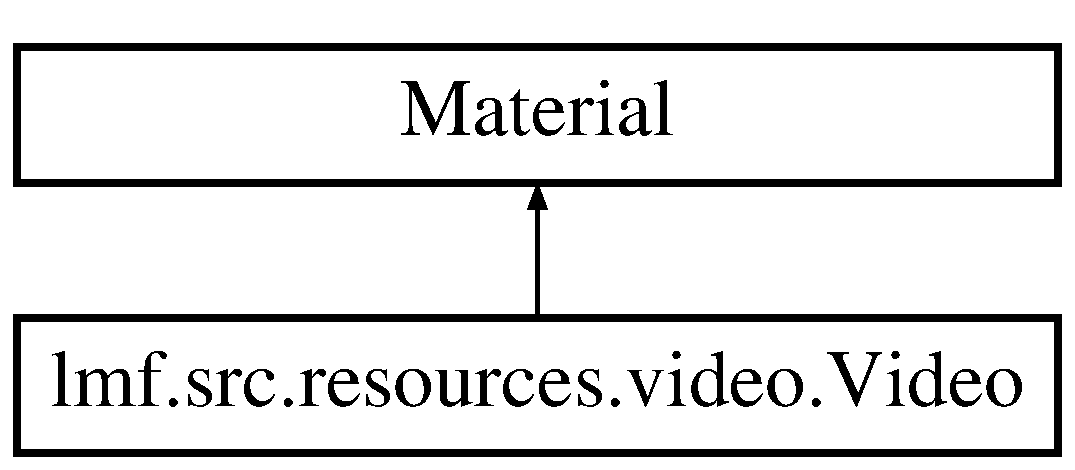
\includegraphics[height=2.000000cm]{classlmf_1_1src_1_1resources_1_1video_1_1_video}
\end{center}
\end{figure}
\subsection*{Public Member Functions}
\begin{DoxyCompactItemize}
\item 
def \hyperlink{classlmf_1_1src_1_1resources_1_1video_1_1_video_a462c094b953b8c030b557184708222cd}{\+\_\+\+\_\+init\+\_\+\+\_\+}
\begin{DoxyCompactList}\small\item\em Constructor. \end{DoxyCompactList}\item 
def \hyperlink{classlmf_1_1src_1_1resources_1_1video_1_1_video_a2926a640d348c5cadf03c67cba87de0a}{\+\_\+\+\_\+del\+\_\+\+\_\+}
\begin{DoxyCompactList}\small\item\em Destructor. \end{DoxyCompactList}\end{DoxyCompactItemize}
\subsection*{Public Attributes}
\begin{DoxyCompactItemize}
\item 
\hyperlink{classlmf_1_1src_1_1resources_1_1video_1_1_video_a21f39ce29f1958b3c82169eabbffc34d}{description}
\end{DoxyCompactItemize}


\subsection{Detailed Description}
\hyperlink{classlmf_1_1src_1_1resources_1_1video_1_1_video}{Video} is a Material subclass representing a video. 

Definition at line 8 of file video.\+py.



\subsection{Constructor \& Destructor Documentation}
\hypertarget{classlmf_1_1src_1_1resources_1_1video_1_1_video_a462c094b953b8c030b557184708222cd}{\index{lmf\+::src\+::resources\+::video\+::\+Video@{lmf\+::src\+::resources\+::video\+::\+Video}!\+\_\+\+\_\+init\+\_\+\+\_\+@{\+\_\+\+\_\+init\+\_\+\+\_\+}}
\index{\+\_\+\+\_\+init\+\_\+\+\_\+@{\+\_\+\+\_\+init\+\_\+\+\_\+}!lmf\+::src\+::resources\+::video\+::\+Video@{lmf\+::src\+::resources\+::video\+::\+Video}}
\subsubsection[{\+\_\+\+\_\+init\+\_\+\+\_\+}]{\setlength{\rightskip}{0pt plus 5cm}def lmf.\+src.\+resources.\+video.\+Video.\+\_\+\+\_\+init\+\_\+\+\_\+ (
\begin{DoxyParamCaption}
\item[{}]{self}
\end{DoxyParamCaption}
)}}\label{classlmf_1_1src_1_1resources_1_1video_1_1_video_a462c094b953b8c030b557184708222cd}


Constructor. 

\hyperlink{classlmf_1_1src_1_1resources_1_1video_1_1_video}{Video} instances are owned by ?. \begin{DoxyReturn}{Returns}
A \hyperlink{classlmf_1_1src_1_1resources_1_1video_1_1_video}{Video} instance. 
\end{DoxyReturn}


Definition at line 11 of file video.\+py.

\hypertarget{classlmf_1_1src_1_1resources_1_1video_1_1_video_a2926a640d348c5cadf03c67cba87de0a}{\index{lmf\+::src\+::resources\+::video\+::\+Video@{lmf\+::src\+::resources\+::video\+::\+Video}!\+\_\+\+\_\+del\+\_\+\+\_\+@{\+\_\+\+\_\+del\+\_\+\+\_\+}}
\index{\+\_\+\+\_\+del\+\_\+\+\_\+@{\+\_\+\+\_\+del\+\_\+\+\_\+}!lmf\+::src\+::resources\+::video\+::\+Video@{lmf\+::src\+::resources\+::video\+::\+Video}}
\subsubsection[{\+\_\+\+\_\+del\+\_\+\+\_\+}]{\setlength{\rightskip}{0pt plus 5cm}def lmf.\+src.\+resources.\+video.\+Video.\+\_\+\+\_\+del\+\_\+\+\_\+ (
\begin{DoxyParamCaption}
\item[{}]{self}
\end{DoxyParamCaption}
)}}\label{classlmf_1_1src_1_1resources_1_1video_1_1_video_a2926a640d348c5cadf03c67cba87de0a}


Destructor. 



Definition at line 20 of file video.\+py.



\subsection{Member Data Documentation}
\hypertarget{classlmf_1_1src_1_1resources_1_1video_1_1_video_a21f39ce29f1958b3c82169eabbffc34d}{\index{lmf\+::src\+::resources\+::video\+::\+Video@{lmf\+::src\+::resources\+::video\+::\+Video}!description@{description}}
\index{description@{description}!lmf\+::src\+::resources\+::video\+::\+Video@{lmf\+::src\+::resources\+::video\+::\+Video}}
\subsubsection[{description}]{\setlength{\rightskip}{0pt plus 5cm}lmf.\+src.\+resources.\+video.\+Video.\+description}}\label{classlmf_1_1src_1_1resources_1_1video_1_1_video_a21f39ce29f1958b3c82169eabbffc34d}


Definition at line 18 of file video.\+py.



The documentation for this class was generated from the following file\+:\begin{DoxyCompactItemize}
\item 
/\+Users/celine/\+Work/\+C\+N\+R\+S/workspace/\+Himal\+Co/dev/lib/lmf/src/resources/\hyperlink{video_8py}{video.\+py}\end{DoxyCompactItemize}

\hypertarget{classlmf_1_1src_1_1utils_1_1error__handling_1_1_warning}{\section{lmf.\+src.\+utils.\+error\+\_\+handling.\+Warning Class Reference}
\label{classlmf_1_1src_1_1utils_1_1error__handling_1_1_warning}\index{lmf.\+src.\+utils.\+error\+\_\+handling.\+Warning@{lmf.\+src.\+utils.\+error\+\_\+handling.\+Warning}}
}


Base class for warnings in this library.  


Inheritance diagram for lmf.\+src.\+utils.\+error\+\_\+handling.\+Warning\+:\begin{figure}[H]
\begin{center}
\leavevmode
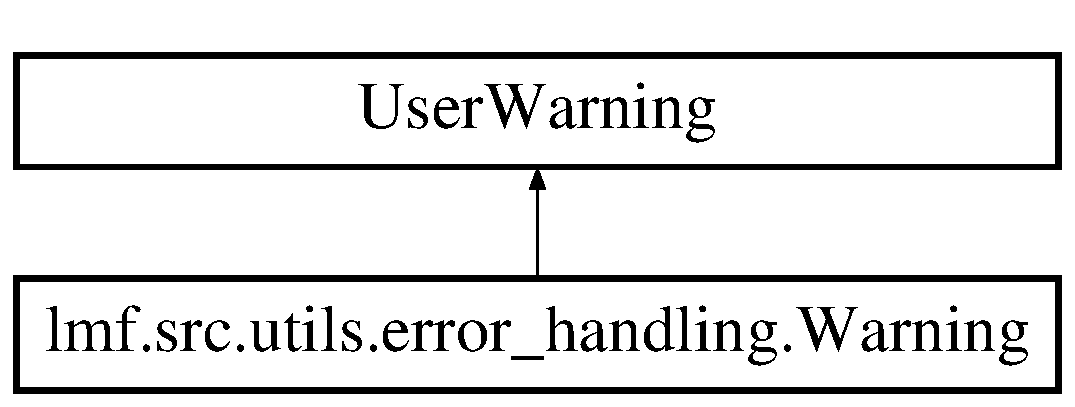
\includegraphics[height=2.000000cm]{classlmf_1_1src_1_1utils_1_1error__handling_1_1_warning}
\end{center}
\end{figure}
\subsection*{Public Member Functions}
\begin{DoxyCompactItemize}
\item 
def \hyperlink{classlmf_1_1src_1_1utils_1_1error__handling_1_1_warning_a1ca035181464bbf15ed05f00ed430384}{\+\_\+\+\_\+init\+\_\+\+\_\+}
\begin{DoxyCompactList}\small\item\em Constructor. \end{DoxyCompactList}\item 
def \hyperlink{classlmf_1_1src_1_1utils_1_1error__handling_1_1_warning_a3dd52e27b533f30681c500081cac6982}{\+\_\+\+\_\+str\+\_\+\+\_\+}
\begin{DoxyCompactList}\small\item\em Build the string to be displayed. \end{DoxyCompactList}\end{DoxyCompactItemize}
\subsection*{Public Attributes}
\begin{DoxyCompactItemize}
\item 
\hyperlink{classlmf_1_1src_1_1utils_1_1error__handling_1_1_warning_a0933de123c20a65d4226d8294d1e3506}{msg}
\item 
\hyperlink{classlmf_1_1src_1_1utils_1_1error__handling_1_1_warning_abfcf05ce22e0fb5e6b81f167729c09c7}{frame\+\_\+info}
\end{DoxyCompactItemize}


\subsection{Detailed Description}
Base class for warnings in this library. 

Definition at line 97 of file error\+\_\+handling.\+py.



\subsection{Constructor \& Destructor Documentation}
\hypertarget{classlmf_1_1src_1_1utils_1_1error__handling_1_1_warning_a1ca035181464bbf15ed05f00ed430384}{\index{lmf\+::src\+::utils\+::error\+\_\+handling\+::\+Warning@{lmf\+::src\+::utils\+::error\+\_\+handling\+::\+Warning}!\+\_\+\+\_\+init\+\_\+\+\_\+@{\+\_\+\+\_\+init\+\_\+\+\_\+}}
\index{\+\_\+\+\_\+init\+\_\+\+\_\+@{\+\_\+\+\_\+init\+\_\+\+\_\+}!lmf\+::src\+::utils\+::error\+\_\+handling\+::\+Warning@{lmf\+::src\+::utils\+::error\+\_\+handling\+::\+Warning}}
\subsubsection[{\+\_\+\+\_\+init\+\_\+\+\_\+}]{\setlength{\rightskip}{0pt plus 5cm}def lmf.\+src.\+utils.\+error\+\_\+handling.\+Warning.\+\_\+\+\_\+init\+\_\+\+\_\+ (
\begin{DoxyParamCaption}
\item[{}]{self, }
\item[{}]{msg}
\end{DoxyParamCaption}
)}}\label{classlmf_1_1src_1_1utils_1_1error__handling_1_1_warning_a1ca035181464bbf15ed05f00ed430384}


Constructor. 


\begin{DoxyParams}{Parameters}
{\em msg} & String to be reported to user. \\
\hline
\end{DoxyParams}
\begin{DoxyReturn}{Returns}
A \hyperlink{classlmf_1_1src_1_1utils_1_1error__handling_1_1_warning}{Warning} instance. 
\end{DoxyReturn}


Definition at line 100 of file error\+\_\+handling.\+py.



\subsection{Member Function Documentation}
\hypertarget{classlmf_1_1src_1_1utils_1_1error__handling_1_1_warning_a3dd52e27b533f30681c500081cac6982}{\index{lmf\+::src\+::utils\+::error\+\_\+handling\+::\+Warning@{lmf\+::src\+::utils\+::error\+\_\+handling\+::\+Warning}!\+\_\+\+\_\+str\+\_\+\+\_\+@{\+\_\+\+\_\+str\+\_\+\+\_\+}}
\index{\+\_\+\+\_\+str\+\_\+\+\_\+@{\+\_\+\+\_\+str\+\_\+\+\_\+}!lmf\+::src\+::utils\+::error\+\_\+handling\+::\+Warning@{lmf\+::src\+::utils\+::error\+\_\+handling\+::\+Warning}}
\subsubsection[{\+\_\+\+\_\+str\+\_\+\+\_\+}]{\setlength{\rightskip}{0pt plus 5cm}def lmf.\+src.\+utils.\+error\+\_\+handling.\+Warning.\+\_\+\+\_\+str\+\_\+\+\_\+ (
\begin{DoxyParamCaption}
\item[{}]{self}
\end{DoxyParamCaption}
)}}\label{classlmf_1_1src_1_1utils_1_1error__handling_1_1_warning_a3dd52e27b533f30681c500081cac6982}


Build the string to be displayed. 

\begin{DoxyReturn}{Returns}
A Python string. 
\end{DoxyReturn}


Definition at line 110 of file error\+\_\+handling.\+py.



\subsection{Member Data Documentation}
\hypertarget{classlmf_1_1src_1_1utils_1_1error__handling_1_1_warning_abfcf05ce22e0fb5e6b81f167729c09c7}{\index{lmf\+::src\+::utils\+::error\+\_\+handling\+::\+Warning@{lmf\+::src\+::utils\+::error\+\_\+handling\+::\+Warning}!frame\+\_\+info@{frame\+\_\+info}}
\index{frame\+\_\+info@{frame\+\_\+info}!lmf\+::src\+::utils\+::error\+\_\+handling\+::\+Warning@{lmf\+::src\+::utils\+::error\+\_\+handling\+::\+Warning}}
\subsubsection[{frame\+\_\+info}]{\setlength{\rightskip}{0pt plus 5cm}lmf.\+src.\+utils.\+error\+\_\+handling.\+Warning.\+frame\+\_\+info}}\label{classlmf_1_1src_1_1utils_1_1error__handling_1_1_warning_abfcf05ce22e0fb5e6b81f167729c09c7}


Definition at line 108 of file error\+\_\+handling.\+py.

\hypertarget{classlmf_1_1src_1_1utils_1_1error__handling_1_1_warning_a0933de123c20a65d4226d8294d1e3506}{\index{lmf\+::src\+::utils\+::error\+\_\+handling\+::\+Warning@{lmf\+::src\+::utils\+::error\+\_\+handling\+::\+Warning}!msg@{msg}}
\index{msg@{msg}!lmf\+::src\+::utils\+::error\+\_\+handling\+::\+Warning@{lmf\+::src\+::utils\+::error\+\_\+handling\+::\+Warning}}
\subsubsection[{msg}]{\setlength{\rightskip}{0pt plus 5cm}lmf.\+src.\+utils.\+error\+\_\+handling.\+Warning.\+msg}}\label{classlmf_1_1src_1_1utils_1_1error__handling_1_1_warning_a0933de123c20a65d4226d8294d1e3506}


Definition at line 105 of file error\+\_\+handling.\+py.



The documentation for this class was generated from the following file\+:\begin{DoxyCompactItemize}
\item 
/\+Users/celine/\+Work/\+C\+N\+R\+S/workspace/\+Himal\+Co/dev/lib/lmf/src/utils/\hyperlink{error__handling_8py}{error\+\_\+handling.\+py}\end{DoxyCompactItemize}

\hypertarget{classlmf_1_1src_1_1morphology_1_1word__form_1_1_word_form}{\section{lmf.\+src.\+morphology.\+word\+\_\+form.\+Word\+Form Class Reference}
\label{classlmf_1_1src_1_1morphology_1_1word__form_1_1_word_form}\index{lmf.\+src.\+morphology.\+word\+\_\+form.\+Word\+Form@{lmf.\+src.\+morphology.\+word\+\_\+form.\+Word\+Form}}
}


\char`\"{}\+Word Form is a Form subclass representing a form that a lexeme can take when used in a sentence or a phrase.\char`\"{} (L\+M\+F)  


Inheritance diagram for lmf.\+src.\+morphology.\+word\+\_\+form.\+Word\+Form\+:\begin{figure}[H]
\begin{center}
\leavevmode
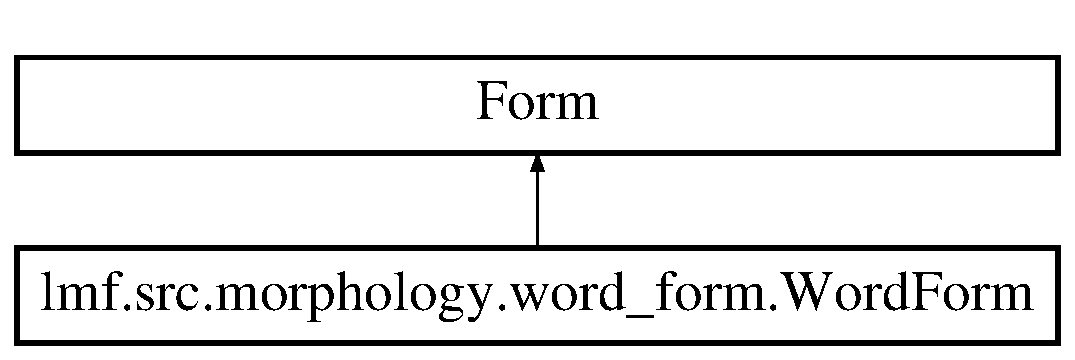
\includegraphics[height=2.000000cm]{classlmf_1_1src_1_1morphology_1_1word__form_1_1_word_form}
\end{center}
\end{figure}
\subsection*{Public Member Functions}
\begin{DoxyCompactItemize}
\item 
def \hyperlink{classlmf_1_1src_1_1morphology_1_1word__form_1_1_word_form_afcc4ec0d271e48a7f35920a1e91aa9b9}{\+\_\+\+\_\+init\+\_\+\+\_\+}
\begin{DoxyCompactList}\small\item\em Constructor. \end{DoxyCompactList}\item 
def \hyperlink{classlmf_1_1src_1_1morphology_1_1word__form_1_1_word_form_aa7b79f6c8c3bd98e57b7d2bc60a9b88c}{\+\_\+\+\_\+del\+\_\+\+\_\+}
\begin{DoxyCompactList}\small\item\em Destructor. \end{DoxyCompactList}\item 
def \hyperlink{classlmf_1_1src_1_1morphology_1_1word__form_1_1_word_form_a35cc3cb1ceda558386c81cf88374b96b}{create\+\_\+form\+\_\+representation}
\begin{DoxyCompactList}\small\item\em Create a form representation. \end{DoxyCompactList}\item 
def \hyperlink{classlmf_1_1src_1_1morphology_1_1word__form_1_1_word_form_a9074b17bb3d1ebcd32b5c8b8fbc3eeda}{add\+\_\+form\+\_\+representation}
\begin{DoxyCompactList}\small\item\em Add a form representation to the word form. \end{DoxyCompactList}\item 
def \hyperlink{classlmf_1_1src_1_1morphology_1_1word__form_1_1_word_form_af5ca5e6fdf8232fb5354b2d5e520f372}{get\+\_\+form\+\_\+representations}
\begin{DoxyCompactList}\small\item\em Get all form representations maintained by the word form. \end{DoxyCompactList}\item 
def \hyperlink{classlmf_1_1src_1_1morphology_1_1word__form_1_1_word_form_aa4010d675af6deb25bf95e7aa54c3f15}{set\+\_\+variant\+\_\+form}
\begin{DoxyCompactList}\small\item\em Set variant form. \end{DoxyCompactList}\item 
def \hyperlink{classlmf_1_1src_1_1morphology_1_1word__form_1_1_word_form_a983151c5529388c7a3002b3239a98b98}{get\+\_\+variant\+\_\+forms}
\begin{DoxyCompactList}\small\item\em Get all variant forms. \end{DoxyCompactList}\item 
def \hyperlink{classlmf_1_1src_1_1morphology_1_1word__form_1_1_word_form_aae046a3403c0fe9ae8f35289878cba67}{set\+\_\+person}
\begin{DoxyCompactList}\small\item\em Set grammatical person. \end{DoxyCompactList}\item 
def \hyperlink{classlmf_1_1src_1_1morphology_1_1word__form_1_1_word_form_a480a6988b8ca2febc53b5d738ae12fac}{get\+\_\+person}
\begin{DoxyCompactList}\small\item\em Get grammatical person. \end{DoxyCompactList}\item 
def \hyperlink{classlmf_1_1src_1_1morphology_1_1word__form_1_1_word_form_a77770e33a70efbf55aa2279c2dbb1112}{set\+\_\+anymacy}
\begin{DoxyCompactList}\small\item\em Set grammatical anymacy. \end{DoxyCompactList}\item 
def \hyperlink{classlmf_1_1src_1_1morphology_1_1word__form_1_1_word_form_a15a5458e866a9bc063766393f1724618}{get\+\_\+anymacy}
\begin{DoxyCompactList}\small\item\em Get anymacy. \end{DoxyCompactList}\item 
def \hyperlink{classlmf_1_1src_1_1morphology_1_1word__form_1_1_word_form_afba8a8bff098989e06c9fce30e4c8163}{set\+\_\+grammatical\+Number}
\begin{DoxyCompactList}\small\item\em Set grammatical number. \end{DoxyCompactList}\item 
def \hyperlink{classlmf_1_1src_1_1morphology_1_1word__form_1_1_word_form_ae1d604cd7edc889a347d9ce41df150c6}{get\+\_\+grammatical\+Number}
\begin{DoxyCompactList}\small\item\em Get grammatical number. \end{DoxyCompactList}\item 
def \hyperlink{classlmf_1_1src_1_1morphology_1_1word__form_1_1_word_form_a711b4b9fb46e15d8d64c831dd3c73f15}{set\+\_\+clusivity}
\begin{DoxyCompactList}\small\item\em Set grammatical clusivity. \end{DoxyCompactList}\item 
def \hyperlink{classlmf_1_1src_1_1morphology_1_1word__form_1_1_word_form_af7009607358c6be4f37b7708193eb2e7}{get\+\_\+clusivity}
\begin{DoxyCompactList}\small\item\em Get grammatical clusivity. \end{DoxyCompactList}\end{DoxyCompactItemize}
\subsection*{Public Attributes}
\begin{DoxyCompactItemize}
\item 
\hyperlink{classlmf_1_1src_1_1morphology_1_1word__form_1_1_word_form_afa022505f197952b8cf9229e065089c2}{grammatical\+Number}
\item 
\hyperlink{classlmf_1_1src_1_1morphology_1_1word__form_1_1_word_form_ab6f9abda4baef6ac9e61ef377c532279}{grammatical\+Gender}
\item 
\hyperlink{classlmf_1_1src_1_1morphology_1_1word__form_1_1_word_form_a982fc33af45a08aa5a039dc4701c3689}{person}
\item 
\hyperlink{classlmf_1_1src_1_1morphology_1_1word__form_1_1_word_form_aaf6096a08af3e92ad3878b68d2e136d3}{anymacy}
\item 
\hyperlink{classlmf_1_1src_1_1morphology_1_1word__form_1_1_word_form_aafbd3d5422083422a4a9ee9b1379913e}{clusivity}
\item 
\hyperlink{classlmf_1_1src_1_1morphology_1_1word__form_1_1_word_form_aaf6dd6658e2e9014ea0490d0edb6cec8}{tense}
\item 
\hyperlink{classlmf_1_1src_1_1morphology_1_1word__form_1_1_word_form_ac996cb6a252a2e97aea0ba861982a640}{case}
\item 
\hyperlink{classlmf_1_1src_1_1morphology_1_1word__form_1_1_word_form_ae529bc2d6ef927ccb6da6599901dccb2}{degree}
\item 
\hyperlink{classlmf_1_1src_1_1morphology_1_1word__form_1_1_word_form_ac08b72f6837815d9d11d3cb0a36ed932}{voice}
\item 
\hyperlink{classlmf_1_1src_1_1morphology_1_1word__form_1_1_word_form_a47aea97a4bbd8cca9624b0143f639716}{verb\+Form\+Mood}
\end{DoxyCompactItemize}


\subsection{Detailed Description}
\char`\"{}\+Word Form is a Form subclass representing a form that a lexeme can take when used in a sentence or a phrase.\char`\"{} (L\+M\+F) 

Definition at line 12 of file word\+\_\+form.\+py.



\subsection{Constructor \& Destructor Documentation}
\hypertarget{classlmf_1_1src_1_1morphology_1_1word__form_1_1_word_form_afcc4ec0d271e48a7f35920a1e91aa9b9}{\index{lmf\+::src\+::morphology\+::word\+\_\+form\+::\+Word\+Form@{lmf\+::src\+::morphology\+::word\+\_\+form\+::\+Word\+Form}!\+\_\+\+\_\+init\+\_\+\+\_\+@{\+\_\+\+\_\+init\+\_\+\+\_\+}}
\index{\+\_\+\+\_\+init\+\_\+\+\_\+@{\+\_\+\+\_\+init\+\_\+\+\_\+}!lmf\+::src\+::morphology\+::word\+\_\+form\+::\+Word\+Form@{lmf\+::src\+::morphology\+::word\+\_\+form\+::\+Word\+Form}}
\subsubsection[{\+\_\+\+\_\+init\+\_\+\+\_\+}]{\setlength{\rightskip}{0pt plus 5cm}def lmf.\+src.\+morphology.\+word\+\_\+form.\+Word\+Form.\+\_\+\+\_\+init\+\_\+\+\_\+ (
\begin{DoxyParamCaption}
\item[{}]{self}
\end{DoxyParamCaption}
)}}\label{classlmf_1_1src_1_1morphology_1_1word__form_1_1_word_form_afcc4ec0d271e48a7f35920a1e91aa9b9}


Constructor. 

\hyperlink{classlmf_1_1src_1_1morphology_1_1word__form_1_1_word_form}{Word\+Form} instances are owned by Lexical\+Entry. \begin{DoxyReturn}{Returns}
A \hyperlink{classlmf_1_1src_1_1morphology_1_1word__form_1_1_word_form}{Word\+Form} instance. 
\end{DoxyReturn}


Definition at line 15 of file word\+\_\+form.\+py.

\hypertarget{classlmf_1_1src_1_1morphology_1_1word__form_1_1_word_form_aa7b79f6c8c3bd98e57b7d2bc60a9b88c}{\index{lmf\+::src\+::morphology\+::word\+\_\+form\+::\+Word\+Form@{lmf\+::src\+::morphology\+::word\+\_\+form\+::\+Word\+Form}!\+\_\+\+\_\+del\+\_\+\+\_\+@{\+\_\+\+\_\+del\+\_\+\+\_\+}}
\index{\+\_\+\+\_\+del\+\_\+\+\_\+@{\+\_\+\+\_\+del\+\_\+\+\_\+}!lmf\+::src\+::morphology\+::word\+\_\+form\+::\+Word\+Form@{lmf\+::src\+::morphology\+::word\+\_\+form\+::\+Word\+Form}}
\subsubsection[{\+\_\+\+\_\+del\+\_\+\+\_\+}]{\setlength{\rightskip}{0pt plus 5cm}def lmf.\+src.\+morphology.\+word\+\_\+form.\+Word\+Form.\+\_\+\+\_\+del\+\_\+\+\_\+ (
\begin{DoxyParamCaption}
\item[{}]{self}
\end{DoxyParamCaption}
)}}\label{classlmf_1_1src_1_1morphology_1_1word__form_1_1_word_form_aa7b79f6c8c3bd98e57b7d2bc60a9b88c}


Destructor. 



Definition at line 33 of file word\+\_\+form.\+py.



\subsection{Member Function Documentation}
\hypertarget{classlmf_1_1src_1_1morphology_1_1word__form_1_1_word_form_a9074b17bb3d1ebcd32b5c8b8fbc3eeda}{\index{lmf\+::src\+::morphology\+::word\+\_\+form\+::\+Word\+Form@{lmf\+::src\+::morphology\+::word\+\_\+form\+::\+Word\+Form}!add\+\_\+form\+\_\+representation@{add\+\_\+form\+\_\+representation}}
\index{add\+\_\+form\+\_\+representation@{add\+\_\+form\+\_\+representation}!lmf\+::src\+::morphology\+::word\+\_\+form\+::\+Word\+Form@{lmf\+::src\+::morphology\+::word\+\_\+form\+::\+Word\+Form}}
\subsubsection[{add\+\_\+form\+\_\+representation}]{\setlength{\rightskip}{0pt plus 5cm}def lmf.\+src.\+morphology.\+word\+\_\+form.\+Word\+Form.\+add\+\_\+form\+\_\+representation (
\begin{DoxyParamCaption}
\item[{}]{self, }
\item[{}]{form\+\_\+representation}
\end{DoxyParamCaption}
)}}\label{classlmf_1_1src_1_1morphology_1_1word__form_1_1_word_form_a9074b17bb3d1ebcd32b5c8b8fbc3eeda}


Add a form representation to the word form. 


\begin{DoxyParams}{Parameters}
{\em form\+\_\+representation} & The Form\+Representation instance to add to the word form. \\
\hline
\end{DoxyParams}
\begin{DoxyReturn}{Returns}
\hyperlink{classlmf_1_1src_1_1morphology_1_1word__form_1_1_word_form}{Word\+Form} instance. 
\end{DoxyReturn}


Definition at line 44 of file word\+\_\+form.\+py.

\hypertarget{classlmf_1_1src_1_1morphology_1_1word__form_1_1_word_form_a35cc3cb1ceda558386c81cf88374b96b}{\index{lmf\+::src\+::morphology\+::word\+\_\+form\+::\+Word\+Form@{lmf\+::src\+::morphology\+::word\+\_\+form\+::\+Word\+Form}!create\+\_\+form\+\_\+representation@{create\+\_\+form\+\_\+representation}}
\index{create\+\_\+form\+\_\+representation@{create\+\_\+form\+\_\+representation}!lmf\+::src\+::morphology\+::word\+\_\+form\+::\+Word\+Form@{lmf\+::src\+::morphology\+::word\+\_\+form\+::\+Word\+Form}}
\subsubsection[{create\+\_\+form\+\_\+representation}]{\setlength{\rightskip}{0pt plus 5cm}def lmf.\+src.\+morphology.\+word\+\_\+form.\+Word\+Form.\+create\+\_\+form\+\_\+representation (
\begin{DoxyParamCaption}
\item[{}]{self}
\end{DoxyParamCaption}
)}}\label{classlmf_1_1src_1_1morphology_1_1word__form_1_1_word_form_a35cc3cb1ceda558386c81cf88374b96b}


Create a form representation. 

\begin{DoxyReturn}{Returns}
Form\+Representation instance. 
\end{DoxyReturn}


Definition at line 38 of file word\+\_\+form.\+py.

\hypertarget{classlmf_1_1src_1_1morphology_1_1word__form_1_1_word_form_a15a5458e866a9bc063766393f1724618}{\index{lmf\+::src\+::morphology\+::word\+\_\+form\+::\+Word\+Form@{lmf\+::src\+::morphology\+::word\+\_\+form\+::\+Word\+Form}!get\+\_\+anymacy@{get\+\_\+anymacy}}
\index{get\+\_\+anymacy@{get\+\_\+anymacy}!lmf\+::src\+::morphology\+::word\+\_\+form\+::\+Word\+Form@{lmf\+::src\+::morphology\+::word\+\_\+form\+::\+Word\+Form}}
\subsubsection[{get\+\_\+anymacy}]{\setlength{\rightskip}{0pt plus 5cm}def lmf.\+src.\+morphology.\+word\+\_\+form.\+Word\+Form.\+get\+\_\+anymacy (
\begin{DoxyParamCaption}
\item[{}]{self}
\end{DoxyParamCaption}
)}}\label{classlmf_1_1src_1_1morphology_1_1word__form_1_1_word_form_a15a5458e866a9bc063766393f1724618}


Get anymacy. 

\begin{DoxyReturn}{Returns}
\hyperlink{classlmf_1_1src_1_1morphology_1_1word__form_1_1_word_form}{Word\+Form} attribute 'anymacy'. 
\end{DoxyReturn}


Definition at line 116 of file word\+\_\+form.\+py.

\hypertarget{classlmf_1_1src_1_1morphology_1_1word__form_1_1_word_form_af7009607358c6be4f37b7708193eb2e7}{\index{lmf\+::src\+::morphology\+::word\+\_\+form\+::\+Word\+Form@{lmf\+::src\+::morphology\+::word\+\_\+form\+::\+Word\+Form}!get\+\_\+clusivity@{get\+\_\+clusivity}}
\index{get\+\_\+clusivity@{get\+\_\+clusivity}!lmf\+::src\+::morphology\+::word\+\_\+form\+::\+Word\+Form@{lmf\+::src\+::morphology\+::word\+\_\+form\+::\+Word\+Form}}
\subsubsection[{get\+\_\+clusivity}]{\setlength{\rightskip}{0pt plus 5cm}def lmf.\+src.\+morphology.\+word\+\_\+form.\+Word\+Form.\+get\+\_\+clusivity (
\begin{DoxyParamCaption}
\item[{}]{self}
\end{DoxyParamCaption}
)}}\label{classlmf_1_1src_1_1morphology_1_1word__form_1_1_word_form_af7009607358c6be4f37b7708193eb2e7}


Get grammatical clusivity. 

\begin{DoxyReturn}{Returns}
\hyperlink{classlmf_1_1src_1_1morphology_1_1word__form_1_1_word_form}{Word\+Form} attribute 'clusivity'. 
\end{DoxyReturn}


Definition at line 150 of file word\+\_\+form.\+py.

\hypertarget{classlmf_1_1src_1_1morphology_1_1word__form_1_1_word_form_af5ca5e6fdf8232fb5354b2d5e520f372}{\index{lmf\+::src\+::morphology\+::word\+\_\+form\+::\+Word\+Form@{lmf\+::src\+::morphology\+::word\+\_\+form\+::\+Word\+Form}!get\+\_\+form\+\_\+representations@{get\+\_\+form\+\_\+representations}}
\index{get\+\_\+form\+\_\+representations@{get\+\_\+form\+\_\+representations}!lmf\+::src\+::morphology\+::word\+\_\+form\+::\+Word\+Form@{lmf\+::src\+::morphology\+::word\+\_\+form\+::\+Word\+Form}}
\subsubsection[{get\+\_\+form\+\_\+representations}]{\setlength{\rightskip}{0pt plus 5cm}def lmf.\+src.\+morphology.\+word\+\_\+form.\+Word\+Form.\+get\+\_\+form\+\_\+representations (
\begin{DoxyParamCaption}
\item[{}]{self}
\end{DoxyParamCaption}
)}}\label{classlmf_1_1src_1_1morphology_1_1word__form_1_1_word_form_af5ca5e6fdf8232fb5354b2d5e520f372}


Get all form representations maintained by the word form. 

\begin{DoxyReturn}{Returns}
A Python list of form representations. 
\end{DoxyReturn}


Definition at line 52 of file word\+\_\+form.\+py.

\hypertarget{classlmf_1_1src_1_1morphology_1_1word__form_1_1_word_form_ae1d604cd7edc889a347d9ce41df150c6}{\index{lmf\+::src\+::morphology\+::word\+\_\+form\+::\+Word\+Form@{lmf\+::src\+::morphology\+::word\+\_\+form\+::\+Word\+Form}!get\+\_\+grammatical\+Number@{get\+\_\+grammatical\+Number}}
\index{get\+\_\+grammatical\+Number@{get\+\_\+grammatical\+Number}!lmf\+::src\+::morphology\+::word\+\_\+form\+::\+Word\+Form@{lmf\+::src\+::morphology\+::word\+\_\+form\+::\+Word\+Form}}
\subsubsection[{get\+\_\+grammatical\+Number}]{\setlength{\rightskip}{0pt plus 5cm}def lmf.\+src.\+morphology.\+word\+\_\+form.\+Word\+Form.\+get\+\_\+grammatical\+Number (
\begin{DoxyParamCaption}
\item[{}]{self}
\end{DoxyParamCaption}
)}}\label{classlmf_1_1src_1_1morphology_1_1word__form_1_1_word_form_ae1d604cd7edc889a347d9ce41df150c6}


Get grammatical number. 

\begin{DoxyReturn}{Returns}
\hyperlink{classlmf_1_1src_1_1morphology_1_1word__form_1_1_word_form}{Word\+Form} attribute 'grammatical\+Number'. 
\end{DoxyReturn}


Definition at line 133 of file word\+\_\+form.\+py.

\hypertarget{classlmf_1_1src_1_1morphology_1_1word__form_1_1_word_form_a480a6988b8ca2febc53b5d738ae12fac}{\index{lmf\+::src\+::morphology\+::word\+\_\+form\+::\+Word\+Form@{lmf\+::src\+::morphology\+::word\+\_\+form\+::\+Word\+Form}!get\+\_\+person@{get\+\_\+person}}
\index{get\+\_\+person@{get\+\_\+person}!lmf\+::src\+::morphology\+::word\+\_\+form\+::\+Word\+Form@{lmf\+::src\+::morphology\+::word\+\_\+form\+::\+Word\+Form}}
\subsubsection[{get\+\_\+person}]{\setlength{\rightskip}{0pt plus 5cm}def lmf.\+src.\+morphology.\+word\+\_\+form.\+Word\+Form.\+get\+\_\+person (
\begin{DoxyParamCaption}
\item[{}]{self}
\end{DoxyParamCaption}
)}}\label{classlmf_1_1src_1_1morphology_1_1word__form_1_1_word_form_a480a6988b8ca2febc53b5d738ae12fac}


Get grammatical person. 

\begin{DoxyReturn}{Returns}
\hyperlink{classlmf_1_1src_1_1morphology_1_1word__form_1_1_word_form}{Word\+Form} attribute 'person'. 
\end{DoxyReturn}


Definition at line 99 of file word\+\_\+form.\+py.

\hypertarget{classlmf_1_1src_1_1morphology_1_1word__form_1_1_word_form_a983151c5529388c7a3002b3239a98b98}{\index{lmf\+::src\+::morphology\+::word\+\_\+form\+::\+Word\+Form@{lmf\+::src\+::morphology\+::word\+\_\+form\+::\+Word\+Form}!get\+\_\+variant\+\_\+forms@{get\+\_\+variant\+\_\+forms}}
\index{get\+\_\+variant\+\_\+forms@{get\+\_\+variant\+\_\+forms}!lmf\+::src\+::morphology\+::word\+\_\+form\+::\+Word\+Form@{lmf\+::src\+::morphology\+::word\+\_\+form\+::\+Word\+Form}}
\subsubsection[{get\+\_\+variant\+\_\+forms}]{\setlength{\rightskip}{0pt plus 5cm}def lmf.\+src.\+morphology.\+word\+\_\+form.\+Word\+Form.\+get\+\_\+variant\+\_\+forms (
\begin{DoxyParamCaption}
\item[{}]{self}
\end{DoxyParamCaption}
)}}\label{classlmf_1_1src_1_1morphology_1_1word__form_1_1_word_form_a983151c5529388c7a3002b3239a98b98}


Get all variant forms. 

This attribute is owned by Form\+Representation. \begin{DoxyReturn}{Returns}
A Python list of Form\+Representation attributes 'variant\+Form'. 
\end{DoxyReturn}


Definition at line 77 of file word\+\_\+form.\+py.

\hypertarget{classlmf_1_1src_1_1morphology_1_1word__form_1_1_word_form_a77770e33a70efbf55aa2279c2dbb1112}{\index{lmf\+::src\+::morphology\+::word\+\_\+form\+::\+Word\+Form@{lmf\+::src\+::morphology\+::word\+\_\+form\+::\+Word\+Form}!set\+\_\+anymacy@{set\+\_\+anymacy}}
\index{set\+\_\+anymacy@{set\+\_\+anymacy}!lmf\+::src\+::morphology\+::word\+\_\+form\+::\+Word\+Form@{lmf\+::src\+::morphology\+::word\+\_\+form\+::\+Word\+Form}}
\subsubsection[{set\+\_\+anymacy}]{\setlength{\rightskip}{0pt plus 5cm}def lmf.\+src.\+morphology.\+word\+\_\+form.\+Word\+Form.\+set\+\_\+anymacy (
\begin{DoxyParamCaption}
\item[{}]{self, }
\item[{}]{anymacy}
\end{DoxyParamCaption}
)}}\label{classlmf_1_1src_1_1morphology_1_1word__form_1_1_word_form_a77770e33a70efbf55aa2279c2dbb1112}


Set grammatical anymacy. 


\begin{DoxyParams}{Parameters}
{\em anymacy} & The grammatical anymacy to set. \\
\hline
\end{DoxyParams}
\begin{DoxyReturn}{Returns}
\hyperlink{classlmf_1_1src_1_1morphology_1_1word__form_1_1_word_form}{Word\+Form} instance. 
\end{DoxyReturn}


Definition at line 105 of file word\+\_\+form.\+py.

\hypertarget{classlmf_1_1src_1_1morphology_1_1word__form_1_1_word_form_a711b4b9fb46e15d8d64c831dd3c73f15}{\index{lmf\+::src\+::morphology\+::word\+\_\+form\+::\+Word\+Form@{lmf\+::src\+::morphology\+::word\+\_\+form\+::\+Word\+Form}!set\+\_\+clusivity@{set\+\_\+clusivity}}
\index{set\+\_\+clusivity@{set\+\_\+clusivity}!lmf\+::src\+::morphology\+::word\+\_\+form\+::\+Word\+Form@{lmf\+::src\+::morphology\+::word\+\_\+form\+::\+Word\+Form}}
\subsubsection[{set\+\_\+clusivity}]{\setlength{\rightskip}{0pt plus 5cm}def lmf.\+src.\+morphology.\+word\+\_\+form.\+Word\+Form.\+set\+\_\+clusivity (
\begin{DoxyParamCaption}
\item[{}]{self, }
\item[{}]{clusivity}
\end{DoxyParamCaption}
)}}\label{classlmf_1_1src_1_1morphology_1_1word__form_1_1_word_form_a711b4b9fb46e15d8d64c831dd3c73f15}


Set grammatical clusivity. 


\begin{DoxyParams}{Parameters}
{\em clusivity} & The grammatical clusivity to set. \\
\hline
\end{DoxyParams}
\begin{DoxyReturn}{Returns}
\hyperlink{classlmf_1_1src_1_1morphology_1_1word__form_1_1_word_form}{Word\+Form} instance. 
\end{DoxyReturn}


Definition at line 139 of file word\+\_\+form.\+py.

\hypertarget{classlmf_1_1src_1_1morphology_1_1word__form_1_1_word_form_afba8a8bff098989e06c9fce30e4c8163}{\index{lmf\+::src\+::morphology\+::word\+\_\+form\+::\+Word\+Form@{lmf\+::src\+::morphology\+::word\+\_\+form\+::\+Word\+Form}!set\+\_\+grammatical\+Number@{set\+\_\+grammatical\+Number}}
\index{set\+\_\+grammatical\+Number@{set\+\_\+grammatical\+Number}!lmf\+::src\+::morphology\+::word\+\_\+form\+::\+Word\+Form@{lmf\+::src\+::morphology\+::word\+\_\+form\+::\+Word\+Form}}
\subsubsection[{set\+\_\+grammatical\+Number}]{\setlength{\rightskip}{0pt plus 5cm}def lmf.\+src.\+morphology.\+word\+\_\+form.\+Word\+Form.\+set\+\_\+grammatical\+Number (
\begin{DoxyParamCaption}
\item[{}]{self, }
\item[{}]{grammatical\+\_\+number}
\end{DoxyParamCaption}
)}}\label{classlmf_1_1src_1_1morphology_1_1word__form_1_1_word_form_afba8a8bff098989e06c9fce30e4c8163}


Set grammatical number. 


\begin{DoxyParams}{Parameters}
{\em grammatical\+\_\+number} & The grammatical number to set. \\
\hline
\end{DoxyParams}
\begin{DoxyReturn}{Returns}
\hyperlink{classlmf_1_1src_1_1morphology_1_1word__form_1_1_word_form}{Word\+Form} instance. 
\end{DoxyReturn}


Definition at line 122 of file word\+\_\+form.\+py.

\hypertarget{classlmf_1_1src_1_1morphology_1_1word__form_1_1_word_form_aae046a3403c0fe9ae8f35289878cba67}{\index{lmf\+::src\+::morphology\+::word\+\_\+form\+::\+Word\+Form@{lmf\+::src\+::morphology\+::word\+\_\+form\+::\+Word\+Form}!set\+\_\+person@{set\+\_\+person}}
\index{set\+\_\+person@{set\+\_\+person}!lmf\+::src\+::morphology\+::word\+\_\+form\+::\+Word\+Form@{lmf\+::src\+::morphology\+::word\+\_\+form\+::\+Word\+Form}}
\subsubsection[{set\+\_\+person}]{\setlength{\rightskip}{0pt plus 5cm}def lmf.\+src.\+morphology.\+word\+\_\+form.\+Word\+Form.\+set\+\_\+person (
\begin{DoxyParamCaption}
\item[{}]{self, }
\item[{}]{person}
\end{DoxyParamCaption}
)}}\label{classlmf_1_1src_1_1morphology_1_1word__form_1_1_word_form_aae046a3403c0fe9ae8f35289878cba67}


Set grammatical person. 


\begin{DoxyParams}{Parameters}
{\em person} & The grammatical person to set. \\
\hline
\end{DoxyParams}
\begin{DoxyReturn}{Returns}
\hyperlink{classlmf_1_1src_1_1morphology_1_1word__form_1_1_word_form}{Word\+Form} instance. 
\end{DoxyReturn}


Definition at line 88 of file word\+\_\+form.\+py.

\hypertarget{classlmf_1_1src_1_1morphology_1_1word__form_1_1_word_form_aa4010d675af6deb25bf95e7aa54c3f15}{\index{lmf\+::src\+::morphology\+::word\+\_\+form\+::\+Word\+Form@{lmf\+::src\+::morphology\+::word\+\_\+form\+::\+Word\+Form}!set\+\_\+variant\+\_\+form@{set\+\_\+variant\+\_\+form}}
\index{set\+\_\+variant\+\_\+form@{set\+\_\+variant\+\_\+form}!lmf\+::src\+::morphology\+::word\+\_\+form\+::\+Word\+Form@{lmf\+::src\+::morphology\+::word\+\_\+form\+::\+Word\+Form}}
\subsubsection[{set\+\_\+variant\+\_\+form}]{\setlength{\rightskip}{0pt plus 5cm}def lmf.\+src.\+morphology.\+word\+\_\+form.\+Word\+Form.\+set\+\_\+variant\+\_\+form (
\begin{DoxyParamCaption}
\item[{}]{self, }
\item[{}]{variant\+\_\+form}
\end{DoxyParamCaption}
)}}\label{classlmf_1_1src_1_1morphology_1_1word__form_1_1_word_form_aa4010d675af6deb25bf95e7aa54c3f15}


Set variant form. 

This attribute is owned by Form\+Representation. 
\begin{DoxyParams}{Parameters}
{\em variant\+\_\+form} & Variant form. \\
\hline
\end{DoxyParams}
\begin{DoxyReturn}{Returns}
\hyperlink{classlmf_1_1src_1_1morphology_1_1word__form_1_1_word_form}{Word\+Form} instance. 
\end{DoxyReturn}


Definition at line 58 of file word\+\_\+form.\+py.



\subsection{Member Data Documentation}
\hypertarget{classlmf_1_1src_1_1morphology_1_1word__form_1_1_word_form_aaf6096a08af3e92ad3878b68d2e136d3}{\index{lmf\+::src\+::morphology\+::word\+\_\+form\+::\+Word\+Form@{lmf\+::src\+::morphology\+::word\+\_\+form\+::\+Word\+Form}!anymacy@{anymacy}}
\index{anymacy@{anymacy}!lmf\+::src\+::morphology\+::word\+\_\+form\+::\+Word\+Form@{lmf\+::src\+::morphology\+::word\+\_\+form\+::\+Word\+Form}}
\subsubsection[{anymacy}]{\setlength{\rightskip}{0pt plus 5cm}lmf.\+src.\+morphology.\+word\+\_\+form.\+Word\+Form.\+anymacy}}\label{classlmf_1_1src_1_1morphology_1_1word__form_1_1_word_form_aaf6096a08af3e92ad3878b68d2e136d3}


Definition at line 25 of file word\+\_\+form.\+py.

\hypertarget{classlmf_1_1src_1_1morphology_1_1word__form_1_1_word_form_ac996cb6a252a2e97aea0ba861982a640}{\index{lmf\+::src\+::morphology\+::word\+\_\+form\+::\+Word\+Form@{lmf\+::src\+::morphology\+::word\+\_\+form\+::\+Word\+Form}!case@{case}}
\index{case@{case}!lmf\+::src\+::morphology\+::word\+\_\+form\+::\+Word\+Form@{lmf\+::src\+::morphology\+::word\+\_\+form\+::\+Word\+Form}}
\subsubsection[{case}]{\setlength{\rightskip}{0pt plus 5cm}lmf.\+src.\+morphology.\+word\+\_\+form.\+Word\+Form.\+case}}\label{classlmf_1_1src_1_1morphology_1_1word__form_1_1_word_form_ac996cb6a252a2e97aea0ba861982a640}


Definition at line 28 of file word\+\_\+form.\+py.

\hypertarget{classlmf_1_1src_1_1morphology_1_1word__form_1_1_word_form_aafbd3d5422083422a4a9ee9b1379913e}{\index{lmf\+::src\+::morphology\+::word\+\_\+form\+::\+Word\+Form@{lmf\+::src\+::morphology\+::word\+\_\+form\+::\+Word\+Form}!clusivity@{clusivity}}
\index{clusivity@{clusivity}!lmf\+::src\+::morphology\+::word\+\_\+form\+::\+Word\+Form@{lmf\+::src\+::morphology\+::word\+\_\+form\+::\+Word\+Form}}
\subsubsection[{clusivity}]{\setlength{\rightskip}{0pt plus 5cm}lmf.\+src.\+morphology.\+word\+\_\+form.\+Word\+Form.\+clusivity}}\label{classlmf_1_1src_1_1morphology_1_1word__form_1_1_word_form_aafbd3d5422083422a4a9ee9b1379913e}


Definition at line 26 of file word\+\_\+form.\+py.

\hypertarget{classlmf_1_1src_1_1morphology_1_1word__form_1_1_word_form_ae529bc2d6ef927ccb6da6599901dccb2}{\index{lmf\+::src\+::morphology\+::word\+\_\+form\+::\+Word\+Form@{lmf\+::src\+::morphology\+::word\+\_\+form\+::\+Word\+Form}!degree@{degree}}
\index{degree@{degree}!lmf\+::src\+::morphology\+::word\+\_\+form\+::\+Word\+Form@{lmf\+::src\+::morphology\+::word\+\_\+form\+::\+Word\+Form}}
\subsubsection[{degree}]{\setlength{\rightskip}{0pt plus 5cm}lmf.\+src.\+morphology.\+word\+\_\+form.\+Word\+Form.\+degree}}\label{classlmf_1_1src_1_1morphology_1_1word__form_1_1_word_form_ae529bc2d6ef927ccb6da6599901dccb2}


Definition at line 29 of file word\+\_\+form.\+py.

\hypertarget{classlmf_1_1src_1_1morphology_1_1word__form_1_1_word_form_ab6f9abda4baef6ac9e61ef377c532279}{\index{lmf\+::src\+::morphology\+::word\+\_\+form\+::\+Word\+Form@{lmf\+::src\+::morphology\+::word\+\_\+form\+::\+Word\+Form}!grammatical\+Gender@{grammatical\+Gender}}
\index{grammatical\+Gender@{grammatical\+Gender}!lmf\+::src\+::morphology\+::word\+\_\+form\+::\+Word\+Form@{lmf\+::src\+::morphology\+::word\+\_\+form\+::\+Word\+Form}}
\subsubsection[{grammatical\+Gender}]{\setlength{\rightskip}{0pt plus 5cm}lmf.\+src.\+morphology.\+word\+\_\+form.\+Word\+Form.\+grammatical\+Gender}}\label{classlmf_1_1src_1_1morphology_1_1word__form_1_1_word_form_ab6f9abda4baef6ac9e61ef377c532279}


Definition at line 23 of file word\+\_\+form.\+py.

\hypertarget{classlmf_1_1src_1_1morphology_1_1word__form_1_1_word_form_afa022505f197952b8cf9229e065089c2}{\index{lmf\+::src\+::morphology\+::word\+\_\+form\+::\+Word\+Form@{lmf\+::src\+::morphology\+::word\+\_\+form\+::\+Word\+Form}!grammatical\+Number@{grammatical\+Number}}
\index{grammatical\+Number@{grammatical\+Number}!lmf\+::src\+::morphology\+::word\+\_\+form\+::\+Word\+Form@{lmf\+::src\+::morphology\+::word\+\_\+form\+::\+Word\+Form}}
\subsubsection[{grammatical\+Number}]{\setlength{\rightskip}{0pt plus 5cm}lmf.\+src.\+morphology.\+word\+\_\+form.\+Word\+Form.\+grammatical\+Number}}\label{classlmf_1_1src_1_1morphology_1_1word__form_1_1_word_form_afa022505f197952b8cf9229e065089c2}


Definition at line 22 of file word\+\_\+form.\+py.

\hypertarget{classlmf_1_1src_1_1morphology_1_1word__form_1_1_word_form_a982fc33af45a08aa5a039dc4701c3689}{\index{lmf\+::src\+::morphology\+::word\+\_\+form\+::\+Word\+Form@{lmf\+::src\+::morphology\+::word\+\_\+form\+::\+Word\+Form}!person@{person}}
\index{person@{person}!lmf\+::src\+::morphology\+::word\+\_\+form\+::\+Word\+Form@{lmf\+::src\+::morphology\+::word\+\_\+form\+::\+Word\+Form}}
\subsubsection[{person}]{\setlength{\rightskip}{0pt plus 5cm}lmf.\+src.\+morphology.\+word\+\_\+form.\+Word\+Form.\+person}}\label{classlmf_1_1src_1_1morphology_1_1word__form_1_1_word_form_a982fc33af45a08aa5a039dc4701c3689}


Definition at line 24 of file word\+\_\+form.\+py.

\hypertarget{classlmf_1_1src_1_1morphology_1_1word__form_1_1_word_form_aaf6dd6658e2e9014ea0490d0edb6cec8}{\index{lmf\+::src\+::morphology\+::word\+\_\+form\+::\+Word\+Form@{lmf\+::src\+::morphology\+::word\+\_\+form\+::\+Word\+Form}!tense@{tense}}
\index{tense@{tense}!lmf\+::src\+::morphology\+::word\+\_\+form\+::\+Word\+Form@{lmf\+::src\+::morphology\+::word\+\_\+form\+::\+Word\+Form}}
\subsubsection[{tense}]{\setlength{\rightskip}{0pt plus 5cm}lmf.\+src.\+morphology.\+word\+\_\+form.\+Word\+Form.\+tense}}\label{classlmf_1_1src_1_1morphology_1_1word__form_1_1_word_form_aaf6dd6658e2e9014ea0490d0edb6cec8}


Definition at line 27 of file word\+\_\+form.\+py.

\hypertarget{classlmf_1_1src_1_1morphology_1_1word__form_1_1_word_form_a47aea97a4bbd8cca9624b0143f639716}{\index{lmf\+::src\+::morphology\+::word\+\_\+form\+::\+Word\+Form@{lmf\+::src\+::morphology\+::word\+\_\+form\+::\+Word\+Form}!verb\+Form\+Mood@{verb\+Form\+Mood}}
\index{verb\+Form\+Mood@{verb\+Form\+Mood}!lmf\+::src\+::morphology\+::word\+\_\+form\+::\+Word\+Form@{lmf\+::src\+::morphology\+::word\+\_\+form\+::\+Word\+Form}}
\subsubsection[{verb\+Form\+Mood}]{\setlength{\rightskip}{0pt plus 5cm}lmf.\+src.\+morphology.\+word\+\_\+form.\+Word\+Form.\+verb\+Form\+Mood}}\label{classlmf_1_1src_1_1morphology_1_1word__form_1_1_word_form_a47aea97a4bbd8cca9624b0143f639716}


Definition at line 31 of file word\+\_\+form.\+py.

\hypertarget{classlmf_1_1src_1_1morphology_1_1word__form_1_1_word_form_ac08b72f6837815d9d11d3cb0a36ed932}{\index{lmf\+::src\+::morphology\+::word\+\_\+form\+::\+Word\+Form@{lmf\+::src\+::morphology\+::word\+\_\+form\+::\+Word\+Form}!voice@{voice}}
\index{voice@{voice}!lmf\+::src\+::morphology\+::word\+\_\+form\+::\+Word\+Form@{lmf\+::src\+::morphology\+::word\+\_\+form\+::\+Word\+Form}}
\subsubsection[{voice}]{\setlength{\rightskip}{0pt plus 5cm}lmf.\+src.\+morphology.\+word\+\_\+form.\+Word\+Form.\+voice}}\label{classlmf_1_1src_1_1morphology_1_1word__form_1_1_word_form_ac08b72f6837815d9d11d3cb0a36ed932}


Definition at line 30 of file word\+\_\+form.\+py.



The documentation for this class was generated from the following file\+:\begin{DoxyCompactItemize}
\item 
/\+Users/celine/\+Work/\+C\+N\+R\+S/workspace/\+Himal\+Co/dev/lib/lmf/src/morphology/\hyperlink{word__form_8py}{word\+\_\+form.\+py}\end{DoxyCompactItemize}

\chapter{File Documentation}
\hypertarget{____init_____8py}{\section{/\+Users/celine/\+Work/\+C\+N\+R\+S/workspace/\+Himal\+Co/dev/lib/lmf/src/\+\_\+\+\_\+init\+\_\+\+\_\+.py File Reference}
\label{____init_____8py}\index{/\+Users/celine/\+Work/\+C\+N\+R\+S/workspace/\+Himal\+Co/dev/lib/lmf/src/\+\_\+\+\_\+init\+\_\+\+\_\+.\+py@{/\+Users/celine/\+Work/\+C\+N\+R\+S/workspace/\+Himal\+Co/dev/lib/lmf/src/\+\_\+\+\_\+init\+\_\+\+\_\+.\+py}}
}
\subsection*{Namespaces}
\begin{DoxyCompactItemize}
\item 
 \hyperlink{namespacelmf_1_1src}{lmf.\+src}
\end{DoxyCompactItemize}

\hypertarget{common_2____init_____8py}{\section{/\+Users/celine/\+Work/\+C\+N\+R\+S/workspace/\+Himal\+Co/dev/lib/lmf/src/common/\+\_\+\+\_\+init\+\_\+\+\_\+.py File Reference}
\label{common_2____init_____8py}\index{/\+Users/celine/\+Work/\+C\+N\+R\+S/workspace/\+Himal\+Co/dev/lib/lmf/src/common/\+\_\+\+\_\+init\+\_\+\+\_\+.\+py@{/\+Users/celine/\+Work/\+C\+N\+R\+S/workspace/\+Himal\+Co/dev/lib/lmf/src/common/\+\_\+\+\_\+init\+\_\+\+\_\+.\+py}}
}
\subsection*{Namespaces}
\begin{DoxyCompactItemize}
\item 
 \hyperlink{namespacelmf_1_1src_1_1common}{lmf.\+src.\+common}
\end{DoxyCompactItemize}

\hypertarget{config_2____init_____8py}{\section{/\+Users/celine/\+Work/\+C\+N\+R\+S/workspace/\+Himal\+Co/dev/lib/lmf/src/config/\+\_\+\+\_\+init\+\_\+\+\_\+.py File Reference}
\label{config_2____init_____8py}\index{/\+Users/celine/\+Work/\+C\+N\+R\+S/workspace/\+Himal\+Co/dev/lib/lmf/src/config/\+\_\+\+\_\+init\+\_\+\+\_\+.\+py@{/\+Users/celine/\+Work/\+C\+N\+R\+S/workspace/\+Himal\+Co/dev/lib/lmf/src/config/\+\_\+\+\_\+init\+\_\+\+\_\+.\+py}}
}
\subsection*{Namespaces}
\begin{DoxyCompactItemize}
\item 
 \hyperlink{namespacesrc_1_1config}{src.\+config}
\end{DoxyCompactItemize}

\hypertarget{core_2____init_____8py}{\section{/\+Users/celine/\+Work/\+C\+N\+R\+S/workspace/\+Himal\+Co/dev/lib/lmf/src/core/\+\_\+\+\_\+init\+\_\+\+\_\+.py File Reference}
\label{core_2____init_____8py}\index{/\+Users/celine/\+Work/\+C\+N\+R\+S/workspace/\+Himal\+Co/dev/lib/lmf/src/core/\+\_\+\+\_\+init\+\_\+\+\_\+.\+py@{/\+Users/celine/\+Work/\+C\+N\+R\+S/workspace/\+Himal\+Co/dev/lib/lmf/src/core/\+\_\+\+\_\+init\+\_\+\+\_\+.\+py}}
}
\subsection*{Namespaces}
\begin{DoxyCompactItemize}
\item 
 \hyperlink{namespacelmf_1_1src_1_1core}{lmf.\+src.\+core}
\end{DoxyCompactItemize}

\hypertarget{input_2____init_____8py}{\section{/\+Users/celine/\+Work/\+C\+N\+R\+S/workspace/\+Himal\+Co/dev/lib/lmf/src/input/\+\_\+\+\_\+init\+\_\+\+\_\+.py File Reference}
\label{input_2____init_____8py}\index{/\+Users/celine/\+Work/\+C\+N\+R\+S/workspace/\+Himal\+Co/dev/lib/lmf/src/input/\+\_\+\+\_\+init\+\_\+\+\_\+.\+py@{/\+Users/celine/\+Work/\+C\+N\+R\+S/workspace/\+Himal\+Co/dev/lib/lmf/src/input/\+\_\+\+\_\+init\+\_\+\+\_\+.\+py}}
}
\subsection*{Namespaces}
\begin{DoxyCompactItemize}
\item 
 \hyperlink{namespacesrc_1_1input}{src.\+input}
\end{DoxyCompactItemize}

\hypertarget{morphology_2____init_____8py}{\section{/\+Users/celine/\+Work/\+C\+N\+R\+S/workspace/\+Himal\+Co/dev/lib/lmf/src/morphology/\+\_\+\+\_\+init\+\_\+\+\_\+.py File Reference}
\label{morphology_2____init_____8py}\index{/\+Users/celine/\+Work/\+C\+N\+R\+S/workspace/\+Himal\+Co/dev/lib/lmf/src/morphology/\+\_\+\+\_\+init\+\_\+\+\_\+.\+py@{/\+Users/celine/\+Work/\+C\+N\+R\+S/workspace/\+Himal\+Co/dev/lib/lmf/src/morphology/\+\_\+\+\_\+init\+\_\+\+\_\+.\+py}}
}
\subsection*{Namespaces}
\begin{DoxyCompactItemize}
\item 
 \hyperlink{namespacesrc_1_1morphology}{src.\+morphology}
\end{DoxyCompactItemize}

\hypertarget{morphosyntax_2____init_____8py}{\section{/\+Users/celine/\+Work/\+C\+N\+R\+S/workspace/\+Himal\+Co/dev/lib/lmf/src/morphosyntax/\+\_\+\+\_\+init\+\_\+\+\_\+.py File Reference}
\label{morphosyntax_2____init_____8py}\index{/\+Users/celine/\+Work/\+C\+N\+R\+S/workspace/\+Himal\+Co/dev/lib/lmf/src/morphosyntax/\+\_\+\+\_\+init\+\_\+\+\_\+.\+py@{/\+Users/celine/\+Work/\+C\+N\+R\+S/workspace/\+Himal\+Co/dev/lib/lmf/src/morphosyntax/\+\_\+\+\_\+init\+\_\+\+\_\+.\+py}}
}
\subsection*{Namespaces}
\begin{DoxyCompactItemize}
\item 
 \hyperlink{namespacesrc_1_1morphosyntax}{src.\+morphosyntax}
\end{DoxyCompactItemize}

\hypertarget{mrd_2____init_____8py}{\section{/\+Users/celine/\+Work/\+C\+N\+R\+S/workspace/\+Himal\+Co/dev/lib/lmf/src/mrd/\+\_\+\+\_\+init\+\_\+\+\_\+.py File Reference}
\label{mrd_2____init_____8py}\index{/\+Users/celine/\+Work/\+C\+N\+R\+S/workspace/\+Himal\+Co/dev/lib/lmf/src/mrd/\+\_\+\+\_\+init\+\_\+\+\_\+.\+py@{/\+Users/celine/\+Work/\+C\+N\+R\+S/workspace/\+Himal\+Co/dev/lib/lmf/src/mrd/\+\_\+\+\_\+init\+\_\+\+\_\+.\+py}}
}
\subsection*{Namespaces}
\begin{DoxyCompactItemize}
\item 
 \hyperlink{namespacelmf_1_1src_1_1mrd}{lmf.\+src.\+mrd}
\end{DoxyCompactItemize}

\hypertarget{output_2____init_____8py}{\section{/\+Users/celine/\+Work/\+C\+N\+R\+S/workspace/\+Himal\+Co/dev/lib/lmf/src/output/\+\_\+\+\_\+init\+\_\+\+\_\+.py File Reference}
\label{output_2____init_____8py}\index{/\+Users/celine/\+Work/\+C\+N\+R\+S/workspace/\+Himal\+Co/dev/lib/lmf/src/output/\+\_\+\+\_\+init\+\_\+\+\_\+.\+py@{/\+Users/celine/\+Work/\+C\+N\+R\+S/workspace/\+Himal\+Co/dev/lib/lmf/src/output/\+\_\+\+\_\+init\+\_\+\+\_\+.\+py}}
}
\subsection*{Namespaces}
\begin{DoxyCompactItemize}
\item 
 \hyperlink{namespacesrc_1_1output}{src.\+output}
\end{DoxyCompactItemize}

\hypertarget{resources_2____init_____8py}{\section{/\+Users/celine/\+Work/\+C\+N\+R\+S/workspace/\+Himal\+Co/dev/lib/lmf/src/resources/\+\_\+\+\_\+init\+\_\+\+\_\+.py File Reference}
\label{resources_2____init_____8py}\index{/\+Users/celine/\+Work/\+C\+N\+R\+S/workspace/\+Himal\+Co/dev/lib/lmf/src/resources/\+\_\+\+\_\+init\+\_\+\+\_\+.\+py@{/\+Users/celine/\+Work/\+C\+N\+R\+S/workspace/\+Himal\+Co/dev/lib/lmf/src/resources/\+\_\+\+\_\+init\+\_\+\+\_\+.\+py}}
}
\subsection*{Namespaces}
\begin{DoxyCompactItemize}
\item 
 \hyperlink{namespacesrc_1_1resources}{src.\+resources}
\end{DoxyCompactItemize}

\hypertarget{utils_2____init_____8py}{\section{/\+Users/celine/\+Work/\+C\+N\+R\+S/workspace/\+Himal\+Co/dev/lib/lmf/src/utils/\+\_\+\+\_\+init\+\_\+\+\_\+.py File Reference}
\label{utils_2____init_____8py}\index{/\+Users/celine/\+Work/\+C\+N\+R\+S/workspace/\+Himal\+Co/dev/lib/lmf/src/utils/\+\_\+\+\_\+init\+\_\+\+\_\+.\+py@{/\+Users/celine/\+Work/\+C\+N\+R\+S/workspace/\+Himal\+Co/dev/lib/lmf/src/utils/\+\_\+\+\_\+init\+\_\+\+\_\+.\+py}}
}
\subsection*{Namespaces}
\begin{DoxyCompactItemize}
\item 
 \hyperlink{namespacelmf_1_1src_1_1utils}{lmf.\+src.\+utils}
\end{DoxyCompactItemize}

\hypertarget{range_8py}{\section{/\+Users/celine/\+Work/\+C\+N\+R\+S/workspace/\+Himal\+Co/dev/lib/lmf/src/common/range.py File Reference}
\label{range_8py}\index{/\+Users/celine/\+Work/\+C\+N\+R\+S/workspace/\+Himal\+Co/dev/lib/lmf/src/common/range.\+py@{/\+Users/celine/\+Work/\+C\+N\+R\+S/workspace/\+Himal\+Co/dev/lib/lmf/src/common/range.\+py}}
}
\subsection*{Namespaces}
\begin{DoxyCompactItemize}
\item 
 \hyperlink{namespacelmf_1_1src_1_1common_1_1range}{lmf.\+src.\+common.\+range}
\end{DoxyCompactItemize}
\subsection*{Variables}
\begin{DoxyCompactItemize}
\item 
tuple \hyperlink{namespacelmf_1_1src_1_1common_1_1range_a06c6dcbacac56dba9aaf04fa02b528e1}{lmf.\+src.\+common.\+range.\+part\+Of\+Speech\+\_\+range}
\begin{DoxyCompactList}\small\item\em Possible values allowed for L\+M\+F part of speech Lexical\+Entry attribute. \end{DoxyCompactList}\item 
tuple \hyperlink{namespacelmf_1_1src_1_1common_1_1range_a58f5cff733c3b357e42d3ce87c7080a0}{lmf.\+src.\+common.\+range.\+type\+\_\+variant\+\_\+range}
\begin{DoxyCompactList}\small\item\em Possible values allowed for L\+M\+F variant type Form\+Representation attribute. \end{DoxyCompactList}\item 
tuple \hyperlink{namespacelmf_1_1src_1_1common_1_1range_a042b6a6bbc9e29deed31854fb1767b88}{lmf.\+src.\+common.\+range.\+note\+Type\+\_\+range}
\begin{DoxyCompactList}\small\item\em Possible values allowed for L\+M\+F note type Statement attribute. \end{DoxyCompactList}\item 
tuple \hyperlink{namespacelmf_1_1src_1_1common_1_1range_ae3353d03f04380d7379bd193af24a1ad}{lmf.\+src.\+common.\+range.\+grammatical\+Number\+\_\+range}
\begin{DoxyCompactList}\small\item\em Possible values allowed for L\+M\+F grammatical number Word\+Form attribute. \end{DoxyCompactList}\item 
tuple \hyperlink{namespacelmf_1_1src_1_1common_1_1range_ad872b4a301271d86df2980b34e15ffc4}{lmf.\+src.\+common.\+range.\+grammatical\+Gender\+\_\+range}
\begin{DoxyCompactList}\small\item\em Possible values allowed for L\+M\+F grammatical gender Word\+Form attribute. \end{DoxyCompactList}\item 
tuple \hyperlink{namespacelmf_1_1src_1_1common_1_1range_ad711c6c7c0e62384f61b106ec7bf2af0}{lmf.\+src.\+common.\+range.\+person\+\_\+range}
\begin{DoxyCompactList}\small\item\em Possible values allowed for L\+M\+F grammatical person Word\+Form attribute. \end{DoxyCompactList}\item 
tuple \hyperlink{namespacelmf_1_1src_1_1common_1_1range_a28fddc4c01c49d3a0a5d2446ad9f6edd}{lmf.\+src.\+common.\+range.\+anymacy\+\_\+range}
\begin{DoxyCompactList}\small\item\em Possible values allowed for L\+M\+F anymacy Word\+Form attribute. \end{DoxyCompactList}\item 
tuple \hyperlink{namespacelmf_1_1src_1_1common_1_1range_aa39563f49d7d421ce4b55d2385f3a7f7}{lmf.\+src.\+common.\+range.\+clusivity\+\_\+range}
\begin{DoxyCompactList}\small\item\em Possible values allowed for L\+M\+F clusivity Word\+Form attribute. \end{DoxyCompactList}\item 
tuple \hyperlink{namespacelmf_1_1src_1_1common_1_1range_acc04186fd80669c626821ad13dcb1196}{lmf.\+src.\+common.\+range.\+tense\+\_\+range}
\begin{DoxyCompactList}\small\item\em Possible values allowed for L\+M\+F grammatical tense Word\+Form attribute. \end{DoxyCompactList}\item 
tuple \hyperlink{namespacelmf_1_1src_1_1common_1_1range_a23fdc4c034bc34cab81c6b9c051074dd}{lmf.\+src.\+common.\+range.\+voice\+\_\+range}
\begin{DoxyCompactList}\small\item\em Possible values allowed for L\+M\+F voice Word\+Form attribute. \end{DoxyCompactList}\item 
tuple \hyperlink{namespacelmf_1_1src_1_1common_1_1range_a5a57dc7ed7fa1f785e812cfe2c306ef6}{lmf.\+src.\+common.\+range.\+verb\+Form\+Mood\+\_\+range}
\begin{DoxyCompactList}\small\item\em Possible values allowed for L\+M\+F verb form mood Word\+Form attribute. \end{DoxyCompactList}\item 
tuple \hyperlink{namespacelmf_1_1src_1_1common_1_1range_a38a6c009293e81b8b03b7072692f7a3c}{lmf.\+src.\+common.\+range.\+degree\+\_\+range}
\begin{DoxyCompactList}\small\item\em Possible values allowed for L\+M\+F degree Word\+Form attribute. \end{DoxyCompactList}\item 
tuple \hyperlink{namespacelmf_1_1src_1_1common_1_1range_abab5b7b201360f47699b34e9e685deb6}{lmf.\+src.\+common.\+range.\+semantic\+Relation\+\_\+range}
\begin{DoxyCompactList}\small\item\em Possible values allowed for semantic relation Related\+Form attribute. \end{DoxyCompactList}\item 
tuple \hyperlink{namespacelmf_1_1src_1_1common_1_1range_a9915518fc99ee54c5ac61a23dc12aefe}{lmf.\+src.\+common.\+range.\+paradigm\+Label\+\_\+range}
\begin{DoxyCompactList}\small\item\em Possible values allowed for paradigm label Paradigm attribute. \end{DoxyCompactList}\item 
tuple \hyperlink{namespacelmf_1_1src_1_1common_1_1range_ac02d347b39dab64b3ce3604168d1b652}{lmf.\+src.\+common.\+range.\+type\+\_\+example\+\_\+range}
\begin{DoxyCompactList}\small\item\em Possible values allowed for example type Context attribute. \end{DoxyCompactList}\item 
tuple \hyperlink{namespacelmf_1_1src_1_1common_1_1range_a61963614ed4bb258825e4104a8b47014}{lmf.\+src.\+common.\+range.\+media\+Type\+\_\+range}
\begin{DoxyCompactList}\small\item\em Possible values allowed for media type Material attribute. \end{DoxyCompactList}\item 
tuple \hyperlink{namespacelmf_1_1src_1_1common_1_1range_a6aef6275dfffea6c0ebf4f105ae35b64}{lmf.\+src.\+common.\+range.\+quality\+\_\+range}
\begin{DoxyCompactList}\small\item\em Possible values allowed for quality Audio attribute. \end{DoxyCompactList}\end{DoxyCompactItemize}

\hypertarget{config_2mdf_8py}{\section{/\+Users/celine/\+Work/\+C\+N\+R\+S/workspace/\+Himal\+Co/dev/lib/lmf/src/config/mdf.py File Reference}
\label{config_2mdf_8py}\index{/\+Users/celine/\+Work/\+C\+N\+R\+S/workspace/\+Himal\+Co/dev/lib/lmf/src/config/mdf.\+py@{/\+Users/celine/\+Work/\+C\+N\+R\+S/workspace/\+Himal\+Co/dev/lib/lmf/src/config/mdf.\+py}}
}
\subsection*{Namespaces}
\begin{DoxyCompactItemize}
\item 
 \hyperlink{namespacelmf_1_1src_1_1config_1_1mdf}{lmf.\+src.\+config.\+mdf}
\end{DoxyCompactItemize}
\subsection*{Functions}
\begin{DoxyCompactItemize}
\item 
def \hyperlink{namespacelmf_1_1src_1_1config_1_1mdf_ab9d98a9297210440ed93a3ca490ee7b4}{lmf.\+src.\+config.\+mdf.\+set\+\_\+bw}
\begin{DoxyCompactList}\small\item\em Functions to process some M\+D\+F fields (input) \end{DoxyCompactList}\item 
def \hyperlink{namespacelmf_1_1src_1_1config_1_1mdf_a5af3cc74d2bb8b03d7657c0e7fb3598b}{lmf.\+src.\+config.\+mdf.\+get\+\_\+bw}
\begin{DoxyCompactList}\small\item\em Functions to process some M\+D\+F fields (output) \end{DoxyCompactList}\end{DoxyCompactItemize}
\subsection*{Variables}
\begin{DoxyCompactItemize}
\item 
tuple \hyperlink{namespacelmf_1_1src_1_1config_1_1mdf_a888cd9df8b9511d408e646dc404b5232}{lmf.\+src.\+config.\+mdf.\+mdf\+\_\+lmf}
\begin{DoxyCompactList}\small\item\em Mapping between M\+D\+F markers and L\+M\+F representation (input) \end{DoxyCompactList}\item 
list \hyperlink{namespacelmf_1_1src_1_1config_1_1mdf_afe5efb72442beb65b5083335b744845c}{lmf.\+src.\+config.\+mdf.\+mdf\+\_\+order}
\begin{DoxyCompactList}\small\item\em Order in which M\+D\+F markers must be written (output) This is the standard order defined in Appendix B of \char`\"{}\+Making Dictionaries. A guide to lexicography and the Multi-\/\+Dictionary Formatter\char`\"{}, Software version 1.\+0, David F. \end{DoxyCompactList}\item 
tuple \hyperlink{namespacelmf_1_1src_1_1config_1_1mdf_a78d8f1444783c1b86cbbd91f49a0cd4f}{lmf.\+src.\+config.\+mdf.\+lmf\+\_\+mdf}
\begin{DoxyCompactList}\small\item\em Mapping between L\+M\+F representation and M\+D\+F markers (output) \end{DoxyCompactList}\item 
tuple \hyperlink{namespacelmf_1_1src_1_1config_1_1mdf_a59bb4fce205d8159bc72c946e3855c4a}{lmf.\+src.\+config.\+mdf.\+ps\+\_\+range}
\begin{DoxyCompactList}\small\item\em Possible values allowed for 'ps' M\+D\+F marker. \end{DoxyCompactList}\item 
tuple \hyperlink{namespacelmf_1_1src_1_1config_1_1mdf_a1e76a452fc77f05851e4369134f5980b}{lmf.\+src.\+config.\+mdf.\+ps\+\_\+part\+Of\+Speech}
\begin{DoxyCompactList}\small\item\em Mapping between 'ps' M\+D\+F marker value and L\+M\+F part of speech Lexical\+Entry attribute value (input) Source\+: \href{http://www.isocat.org/rest/dcs/119}{\tt http\+://www.\+isocat.\+org/rest/dcs/119}. \end{DoxyCompactList}\item 
tuple \hyperlink{namespacelmf_1_1src_1_1config_1_1mdf_a20455cbc7aa64cc6eb4ad1749a381738}{lmf.\+src.\+config.\+mdf.\+mdf\+\_\+semantic\+Relation}
\begin{DoxyCompactList}\small\item\em Mapping between M\+D\+F markers and L\+M\+F semantic relation Related\+Form attribute value (input) \end{DoxyCompactList}\item 
tuple \hyperlink{namespacelmf_1_1src_1_1config_1_1mdf_ab58fb9b58bc32ac36efe9b26e4ea3ca2}{lmf.\+src.\+config.\+mdf.\+pd\+\_\+person}
\begin{DoxyCompactList}\small\item\em Mapping between 'pd' M\+D\+F markers and L\+M\+F person Word\+Form attribute value (input) \end{DoxyCompactList}\item 
tuple \hyperlink{namespacelmf_1_1src_1_1config_1_1mdf_a011f241f41e3620deefe53cbb42286b9}{lmf.\+src.\+config.\+mdf.\+pd\+\_\+anymacy}
\begin{DoxyCompactList}\small\item\em Mapping between 'pd' M\+D\+F markers and L\+M\+F anymacy Word\+Form attribute value (input) \end{DoxyCompactList}\item 
tuple \hyperlink{namespacelmf_1_1src_1_1config_1_1mdf_a64be26974728c369cd72ef80bd297154}{lmf.\+src.\+config.\+mdf.\+pd\+\_\+grammatical\+Number}
\begin{DoxyCompactList}\small\item\em Mapping between 'pd' M\+D\+F markers and L\+M\+F grammatical number Word\+Form attribute value (input) \end{DoxyCompactList}\item 
tuple \hyperlink{namespacelmf_1_1src_1_1config_1_1mdf_ac57ebe92cdf841d8d1bfe1e1b94b96bb}{lmf.\+src.\+config.\+mdf.\+pd\+\_\+clusivity}
\begin{DoxyCompactList}\small\item\em Mapping between 'pd' M\+D\+F markers and L\+M\+F clusivity Word\+Form attribute value (input) \end{DoxyCompactList}\item 
tuple \hyperlink{namespacelmf_1_1src_1_1config_1_1mdf_a8e61adc475ca415a33c85ef16c96d03d}{lmf.\+src.\+config.\+mdf.\+pdl\+\_\+paradigm\+Label}
\begin{DoxyCompactList}\small\item\em Mapping between 'pdl' M\+D\+F marker value and L\+M\+F paradigm label Paradigm attribute value (input) \end{DoxyCompactList}\item 
tuple \hyperlink{namespacelmf_1_1src_1_1config_1_1mdf_a69afee1e13ba980f4da1e6d7fb0c488a}{lmf.\+src.\+config.\+mdf.\+sd\+\_\+range}
\begin{DoxyCompactList}\small\item\em Possible values allowed for 'sd' M\+D\+F marker. \end{DoxyCompactList}\item 
tuple \hyperlink{namespacelmf_1_1src_1_1config_1_1mdf_a61a24538d210d4eca3f57f183733fa5a}{lmf.\+src.\+config.\+mdf.\+lf\+\_\+range}
\begin{DoxyCompactList}\small\item\em Possible values allowed for 'lf' M\+D\+F marker. \end{DoxyCompactList}\end{DoxyCompactItemize}

\hypertarget{input_2mdf_8py}{\section{/\+Users/celine/\+Work/\+C\+N\+R\+S/workspace/\+Himal\+Co/dev/lib/lmf/src/input/mdf.py File Reference}
\label{input_2mdf_8py}\index{/\+Users/celine/\+Work/\+C\+N\+R\+S/workspace/\+Himal\+Co/dev/lib/lmf/src/input/mdf.\+py@{/\+Users/celine/\+Work/\+C\+N\+R\+S/workspace/\+Himal\+Co/dev/lib/lmf/src/input/mdf.\+py}}
}
\subsection*{Namespaces}
\begin{DoxyCompactItemize}
\item 
 \hyperlink{namespacelmf_1_1src_1_1input_1_1mdf}{lmf.\+src.\+input.\+mdf}
\end{DoxyCompactItemize}
\subsection*{Functions}
\begin{DoxyCompactItemize}
\item 
def \hyperlink{namespacelmf_1_1src_1_1input_1_1mdf_adf21a8b8bd5a33be054269ced938ba52}{lmf.\+src.\+input.\+mdf.\+mdf\+\_\+read}
\begin{DoxyCompactList}\small\item\em Read an M\+D\+F file. \end{DoxyCompactList}\end{DoxyCompactItemize}

\hypertarget{output_2mdf_8py}{\section{/\+Users/celine/\+Work/\+C\+N\+R\+S/workspace/\+Himal\+Co/dev/lib/lmf/src/output/mdf.py File Reference}
\label{output_2mdf_8py}\index{/\+Users/celine/\+Work/\+C\+N\+R\+S/workspace/\+Himal\+Co/dev/lib/lmf/src/output/mdf.\+py@{/\+Users/celine/\+Work/\+C\+N\+R\+S/workspace/\+Himal\+Co/dev/lib/lmf/src/output/mdf.\+py}}
}
\subsection*{Namespaces}
\begin{DoxyCompactItemize}
\item 
 \hyperlink{namespacesrc_1_1output_1_1mdf}{src.\+output.\+mdf}
\end{DoxyCompactItemize}
\subsection*{Functions}
\begin{DoxyCompactItemize}
\item 
def \hyperlink{namespacesrc_1_1output_1_1mdf_a71397767dc07eda4ff1586de29e7c25d}{src.\+output.\+mdf.\+mdf\+\_\+write}
\begin{DoxyCompactList}\small\item\em Write an M\+D\+F file. \end{DoxyCompactList}\end{DoxyCompactItemize}

\hypertarget{config_2tex_8py}{\section{/\+Users/celine/\+Work/\+C\+N\+R\+S/workspace/\+Himal\+Co/dev/lib/lmf/src/config/tex.py File Reference}
\label{config_2tex_8py}\index{/\+Users/celine/\+Work/\+C\+N\+R\+S/workspace/\+Himal\+Co/dev/lib/lmf/src/config/tex.\+py@{/\+Users/celine/\+Work/\+C\+N\+R\+S/workspace/\+Himal\+Co/dev/lib/lmf/src/config/tex.\+py}}
}
\subsection*{Namespaces}
\begin{DoxyCompactItemize}
\item 
 \hyperlink{namespacelmf_1_1src_1_1config_1_1tex}{lmf.\+src.\+config.\+tex}
\end{DoxyCompactItemize}
\subsection*{Functions}
\begin{DoxyCompactItemize}
\item 
def \hyperlink{namespacelmf_1_1src_1_1config_1_1tex_ac85ca206e865c9cc1d77b77c72a429d2}{lmf.\+src.\+config.\+tex.\+lmf\+\_\+to\+\_\+tex}
\begin{DoxyCompactList}\small\item\em Function giving order in which information must be written in La\+Te\+X and mapping between L\+M\+F representation and La\+Te\+X (output) \end{DoxyCompactList}\end{DoxyCompactItemize}
\subsection*{Variables}
\begin{DoxyCompactItemize}
\item 
tuple \hyperlink{namespacelmf_1_1src_1_1config_1_1tex_a94016d28cbde962dd9dee1465bf19548}{lmf.\+src.\+config.\+tex.\+part\+Of\+Speech\+\_\+tex}
\begin{DoxyCompactList}\small\item\em Mapping between L\+M\+F part of speech Lexical\+Entry attribute value and La\+Te\+X layout (output) \end{DoxyCompactList}\item 
tuple \hyperlink{namespacelmf_1_1src_1_1config_1_1tex_a2a4c92ffc93b18380a5eb8971c518776}{lmf.\+src.\+config.\+tex.\+paradigm\+Label\+\_\+tex}
\begin{DoxyCompactList}\small\item\em Mapping between L\+M\+F paradigm\+Label Paradigm attribute value and La\+Te\+X layout (output) \end{DoxyCompactList}\end{DoxyCompactItemize}

\hypertarget{output_2tex_8py}{\section{/\+Users/celine/\+Work/\+C\+N\+R\+S/workspace/\+Himal\+Co/dev/lib/lmf/src/output/tex.py File Reference}
\label{output_2tex_8py}\index{/\+Users/celine/\+Work/\+C\+N\+R\+S/workspace/\+Himal\+Co/dev/lib/lmf/src/output/tex.\+py@{/\+Users/celine/\+Work/\+C\+N\+R\+S/workspace/\+Himal\+Co/dev/lib/lmf/src/output/tex.\+py}}
}
\subsection*{Namespaces}
\begin{DoxyCompactItemize}
\item 
 \hyperlink{namespacelmf_1_1src_1_1output_1_1tex}{lmf.\+src.\+output.\+tex}
\end{DoxyCompactItemize}
\subsection*{Functions}
\begin{DoxyCompactItemize}
\item 
def \hyperlink{namespacelmf_1_1src_1_1output_1_1tex_ac02be073e031d36d66f61dc7d6fb94df}{lmf.\+src.\+output.\+tex.\+compute\+\_\+header}
\begin{DoxyCompactList}\small\item\em Create La\+Te\+X header. \end{DoxyCompactList}\item 
def \hyperlink{namespacelmf_1_1src_1_1output_1_1tex_a2f69a7ff35d3a419eaa9f4bb40aefa06}{lmf.\+src.\+output.\+tex.\+tex\+\_\+write}
\begin{DoxyCompactList}\small\item\em Write a La\+Te\+X file. \end{DoxyCompactList}\end{DoxyCompactItemize}

\hypertarget{definition_8py}{\section{/\+Users/celine/\+Work/\+C\+N\+R\+S/workspace/\+Himal\+Co/dev/lib/lmf/src/core/definition.py File Reference}
\label{definition_8py}\index{/\+Users/celine/\+Work/\+C\+N\+R\+S/workspace/\+Himal\+Co/dev/lib/lmf/src/core/definition.\+py@{/\+Users/celine/\+Work/\+C\+N\+R\+S/workspace/\+Himal\+Co/dev/lib/lmf/src/core/definition.\+py}}
}
\subsection*{Classes}
\begin{DoxyCompactItemize}
\item 
class \hyperlink{classsrc_1_1core_1_1definition_1_1_definition}{src.\+core.\+definition.\+Definition}
\end{DoxyCompactItemize}
\subsection*{Namespaces}
\begin{DoxyCompactItemize}
\item 
 \hyperlink{namespacesrc_1_1core_1_1definition}{src.\+core.\+definition}
\end{DoxyCompactItemize}

\hypertarget{form_8py}{\section{/\+Users/celine/\+Work/\+C\+N\+R\+S/workspace/\+Himal\+Co/dev/lib/lmf/src/core/form.py File Reference}
\label{form_8py}\index{/\+Users/celine/\+Work/\+C\+N\+R\+S/workspace/\+Himal\+Co/dev/lib/lmf/src/core/form.\+py@{/\+Users/celine/\+Work/\+C\+N\+R\+S/workspace/\+Himal\+Co/dev/lib/lmf/src/core/form.\+py}}
}
\subsection*{Classes}
\begin{DoxyCompactItemize}
\item 
class \hyperlink{classsrc_1_1core_1_1form_1_1_form}{src.\+core.\+form.\+Form}
\end{DoxyCompactItemize}
\subsection*{Namespaces}
\begin{DoxyCompactItemize}
\item 
 \hyperlink{namespacesrc_1_1core_1_1form}{src.\+core.\+form}
\end{DoxyCompactItemize}

\hypertarget{form__representation_8py}{\section{/\+Users/celine/\+Work/\+C\+N\+R\+S/workspace/\+Himal\+Co/dev/lib/lmf/src/core/form\+\_\+representation.py File Reference}
\label{form__representation_8py}\index{/\+Users/celine/\+Work/\+C\+N\+R\+S/workspace/\+Himal\+Co/dev/lib/lmf/src/core/form\+\_\+representation.\+py@{/\+Users/celine/\+Work/\+C\+N\+R\+S/workspace/\+Himal\+Co/dev/lib/lmf/src/core/form\+\_\+representation.\+py}}
}
\subsection*{Classes}
\begin{DoxyCompactItemize}
\item 
class \hyperlink{classlmf_1_1src_1_1core_1_1form__representation_1_1_form_representation}{lmf.\+src.\+core.\+form\+\_\+representation.\+Form\+Representation}
\begin{DoxyCompactList}\small\item\em \char`\"{}\+Form Representation is a class representing one variant orthography of a Form.\char`\"{} (L\+M\+F) \end{DoxyCompactList}\end{DoxyCompactItemize}
\subsection*{Namespaces}
\begin{DoxyCompactItemize}
\item 
 \hyperlink{namespacelmf_1_1src_1_1core_1_1form__representation}{lmf.\+src.\+core.\+form\+\_\+representation}
\end{DoxyCompactItemize}

\hypertarget{global__information_8py}{\section{/\+Users/celine/\+Work/\+C\+N\+R\+S/workspace/\+Himal\+Co/dev/lib/lmf/src/core/global\+\_\+information.py File Reference}
\label{global__information_8py}\index{/\+Users/celine/\+Work/\+C\+N\+R\+S/workspace/\+Himal\+Co/dev/lib/lmf/src/core/global\+\_\+information.\+py@{/\+Users/celine/\+Work/\+C\+N\+R\+S/workspace/\+Himal\+Co/dev/lib/lmf/src/core/global\+\_\+information.\+py}}
}
\subsection*{Classes}
\begin{DoxyCompactItemize}
\item 
class \hyperlink{classsrc_1_1core_1_1global__information_1_1_global_information}{src.\+core.\+global\+\_\+information.\+Global\+Information}
\end{DoxyCompactItemize}
\subsection*{Namespaces}
\begin{DoxyCompactItemize}
\item 
 \hyperlink{namespacesrc_1_1core_1_1global__information}{src.\+core.\+global\+\_\+information}
\end{DoxyCompactItemize}

\hypertarget{lexical__entry_8py}{\section{/\+Users/celine/\+Work/\+C\+N\+R\+S/workspace/\+Himal\+Co/dev/lib/lmf/src/core/lexical\+\_\+entry.py File Reference}
\label{lexical__entry_8py}\index{/\+Users/celine/\+Work/\+C\+N\+R\+S/workspace/\+Himal\+Co/dev/lib/lmf/src/core/lexical\+\_\+entry.\+py@{/\+Users/celine/\+Work/\+C\+N\+R\+S/workspace/\+Himal\+Co/dev/lib/lmf/src/core/lexical\+\_\+entry.\+py}}
}
\subsection*{Classes}
\begin{DoxyCompactItemize}
\item 
class \hyperlink{classlmf_1_1src_1_1core_1_1lexical__entry_1_1_lexical_entry}{lmf.\+src.\+core.\+lexical\+\_\+entry.\+Lexical\+Entry}
\begin{DoxyCompactList}\small\item\em \char`\"{}\+Lexical Entry is a class representing a lexeme in a given language and is a container for managing the Form and Sense classes. A Lexical Entry instance can contain one to many different forms and can have from zero to many different senses.\char`\"{} (L\+M\+F) \end{DoxyCompactList}\end{DoxyCompactItemize}
\subsection*{Namespaces}
\begin{DoxyCompactItemize}
\item 
 \hyperlink{namespacelmf_1_1src_1_1core_1_1lexical__entry}{lmf.\+src.\+core.\+lexical\+\_\+entry}
\end{DoxyCompactItemize}

\hypertarget{lexical__resource_8py}{\section{/\+Users/celine/\+Work/\+C\+N\+R\+S/workspace/\+Himal\+Co/dev/lib/lmf/src/core/lexical\+\_\+resource.py File Reference}
\label{lexical__resource_8py}\index{/\+Users/celine/\+Work/\+C\+N\+R\+S/workspace/\+Himal\+Co/dev/lib/lmf/src/core/lexical\+\_\+resource.\+py@{/\+Users/celine/\+Work/\+C\+N\+R\+S/workspace/\+Himal\+Co/dev/lib/lmf/src/core/lexical\+\_\+resource.\+py}}
}
\subsection*{Classes}
\begin{DoxyCompactItemize}
\item 
class \hyperlink{classlmf_1_1src_1_1core_1_1lexical__resource_1_1_lexical_resource}{lmf.\+src.\+core.\+lexical\+\_\+resource.\+Lexical\+Resource}
\begin{DoxyCompactList}\small\item\em \char`\"{}\+Lexical Resource is a class representing the entire resource and is a container for one or more lexicons. There is only one Lexical Resource instance.\char`\"{} (L\+M\+F) \end{DoxyCompactList}\end{DoxyCompactItemize}
\subsection*{Namespaces}
\begin{DoxyCompactItemize}
\item 
 \hyperlink{namespacelmf_1_1src_1_1core_1_1lexical__resource}{lmf.\+src.\+core.\+lexical\+\_\+resource}
\end{DoxyCompactItemize}

\hypertarget{lexicon_8py}{\section{/\+Users/celine/\+Work/\+C\+N\+R\+S/workspace/\+Himal\+Co/dev/lib/lmf/src/core/lexicon.py File Reference}
\label{lexicon_8py}\index{/\+Users/celine/\+Work/\+C\+N\+R\+S/workspace/\+Himal\+Co/dev/lib/lmf/src/core/lexicon.\+py@{/\+Users/celine/\+Work/\+C\+N\+R\+S/workspace/\+Himal\+Co/dev/lib/lmf/src/core/lexicon.\+py}}
}
\subsection*{Classes}
\begin{DoxyCompactItemize}
\item 
class \hyperlink{classlmf_1_1src_1_1core_1_1lexicon_1_1_lexicon}{lmf.\+src.\+core.\+lexicon.\+Lexicon}
\begin{DoxyCompactList}\small\item\em \char`\"{}\+Lexicon is a class containing all the lexical entries of a given language within the entire resource.\char`\"{} (L\+M\+F) \end{DoxyCompactList}\end{DoxyCompactItemize}
\subsection*{Namespaces}
\begin{DoxyCompactItemize}
\item 
 \hyperlink{namespacelmf_1_1src_1_1core_1_1lexicon}{lmf.\+src.\+core.\+lexicon}
\end{DoxyCompactItemize}

\hypertarget{representation_8py}{\section{/\+Users/celine/\+Work/\+C\+N\+R\+S/workspace/\+Himal\+Co/dev/lib/lmf/src/core/representation.py File Reference}
\label{representation_8py}\index{/\+Users/celine/\+Work/\+C\+N\+R\+S/workspace/\+Himal\+Co/dev/lib/lmf/src/core/representation.\+py@{/\+Users/celine/\+Work/\+C\+N\+R\+S/workspace/\+Himal\+Co/dev/lib/lmf/src/core/representation.\+py}}
}
\subsection*{Classes}
\begin{DoxyCompactItemize}
\item 
class \hyperlink{classlmf_1_1src_1_1core_1_1representation_1_1_representation}{lmf.\+src.\+core.\+representation.\+Representation}
\begin{DoxyCompactList}\small\item\em \char`\"{}\+Representation class is an abstract class representing a Unicode string as well as, if needed, the unique attribute-\/value pairs that describe the specific language, script and orthography.\char`\"{} (L\+M\+F) \end{DoxyCompactList}\end{DoxyCompactItemize}
\subsection*{Namespaces}
\begin{DoxyCompactItemize}
\item 
 \hyperlink{namespacelmf_1_1src_1_1core_1_1representation}{lmf.\+src.\+core.\+representation}
\end{DoxyCompactItemize}

\hypertarget{sense_8py}{\section{/\+Users/celine/\+Work/\+C\+N\+R\+S/workspace/\+Himal\+Co/dev/lib/lmf/src/core/sense.py File Reference}
\label{sense_8py}\index{/\+Users/celine/\+Work/\+C\+N\+R\+S/workspace/\+Himal\+Co/dev/lib/lmf/src/core/sense.\+py@{/\+Users/celine/\+Work/\+C\+N\+R\+S/workspace/\+Himal\+Co/dev/lib/lmf/src/core/sense.\+py}}
}
\subsection*{Classes}
\begin{DoxyCompactItemize}
\item 
class \hyperlink{classlmf_1_1src_1_1core_1_1sense_1_1_sense}{lmf.\+src.\+core.\+sense.\+Sense}
\begin{DoxyCompactList}\small\item\em \char`\"{}\+Sense is a class representing one meaning of a lexical entry. The Sense class allows for hierarchical senses in that a sense may be more specific than another sense of the same lexical entry.\char`\"{} (L\+M\+F) \end{DoxyCompactList}\end{DoxyCompactItemize}
\subsection*{Namespaces}
\begin{DoxyCompactItemize}
\item 
 \hyperlink{namespacelmf_1_1src_1_1core_1_1sense}{lmf.\+src.\+core.\+sense}
\end{DoxyCompactItemize}

\hypertarget{statement_8py}{\section{/\+Users/celine/\+Work/\+C\+N\+R\+S/workspace/\+Himal\+Co/dev/lib/lmf/src/core/statement.py File Reference}
\label{statement_8py}\index{/\+Users/celine/\+Work/\+C\+N\+R\+S/workspace/\+Himal\+Co/dev/lib/lmf/src/core/statement.\+py@{/\+Users/celine/\+Work/\+C\+N\+R\+S/workspace/\+Himal\+Co/dev/lib/lmf/src/core/statement.\+py}}
}
\subsection*{Classes}
\begin{DoxyCompactItemize}
\item 
class \hyperlink{classlmf_1_1src_1_1core_1_1statement_1_1_statement}{lmf.\+src.\+core.\+statement.\+Statement}
\begin{DoxyCompactList}\small\item\em \char`\"{}\+Statement is a class representating a narrative description that refines or complements Definition.\char`\"{} (L\+M\+F) \end{DoxyCompactList}\end{DoxyCompactItemize}
\subsection*{Namespaces}
\begin{DoxyCompactItemize}
\item 
 \hyperlink{namespacelmf_1_1src_1_1core_1_1statement}{lmf.\+src.\+core.\+statement}
\end{DoxyCompactItemize}

\hypertarget{text__representation_8py}{\section{/\+Users/celine/\+Work/\+C\+N\+R\+S/workspace/\+Himal\+Co/dev/lib/lmf/src/core/text\+\_\+representation.py File Reference}
\label{text__representation_8py}\index{/\+Users/celine/\+Work/\+C\+N\+R\+S/workspace/\+Himal\+Co/dev/lib/lmf/src/core/text\+\_\+representation.\+py@{/\+Users/celine/\+Work/\+C\+N\+R\+S/workspace/\+Himal\+Co/dev/lib/lmf/src/core/text\+\_\+representation.\+py}}
}
\subsection*{Classes}
\begin{DoxyCompactItemize}
\item 
class \hyperlink{classsrc_1_1core_1_1text__representation_1_1_text_representation}{src.\+core.\+text\+\_\+representation.\+Text\+Representation}
\end{DoxyCompactItemize}
\subsection*{Namespaces}
\begin{DoxyCompactItemize}
\item 
 \hyperlink{namespacesrc_1_1core_1_1text__representation}{src.\+core.\+text\+\_\+representation}
\end{DoxyCompactItemize}

\hypertarget{elan_8py}{\section{/\+Users/celine/\+Work/\+C\+N\+R\+S/workspace/\+Himal\+Co/dev/lib/lmf/src/input/elan.py File Reference}
\label{elan_8py}\index{/\+Users/celine/\+Work/\+C\+N\+R\+S/workspace/\+Himal\+Co/dev/lib/lmf/src/input/elan.\+py@{/\+Users/celine/\+Work/\+C\+N\+R\+S/workspace/\+Himal\+Co/dev/lib/lmf/src/input/elan.\+py}}
}
\subsection*{Namespaces}
\begin{DoxyCompactItemize}
\item 
 \hyperlink{namespacesrc_1_1input_1_1elan}{src.\+input.\+elan}
\end{DoxyCompactItemize}

\hypertarget{ite_8py}{\section{/\+Users/celine/\+Work/\+C\+N\+R\+S/workspace/\+Himal\+Co/dev/lib/lmf/src/input/ite.py File Reference}
\label{ite_8py}\index{/\+Users/celine/\+Work/\+C\+N\+R\+S/workspace/\+Himal\+Co/dev/lib/lmf/src/input/ite.\+py@{/\+Users/celine/\+Work/\+C\+N\+R\+S/workspace/\+Himal\+Co/dev/lib/lmf/src/input/ite.\+py}}
}
\subsection*{Namespaces}
\begin{DoxyCompactItemize}
\item 
 \hyperlink{namespacelmf_1_1src_1_1input_1_1ite}{lmf.\+src.\+input.\+ite}
\end{DoxyCompactItemize}

\hypertarget{toolbox__settings_8py}{\section{/\+Users/celine/\+Work/\+C\+N\+R\+S/workspace/\+Himal\+Co/dev/lib/lmf/src/input/toolbox\+\_\+settings.py File Reference}
\label{toolbox__settings_8py}\index{/\+Users/celine/\+Work/\+C\+N\+R\+S/workspace/\+Himal\+Co/dev/lib/lmf/src/input/toolbox\+\_\+settings.\+py@{/\+Users/celine/\+Work/\+C\+N\+R\+S/workspace/\+Himal\+Co/dev/lib/lmf/src/input/toolbox\+\_\+settings.\+py}}
}
\subsection*{Namespaces}
\begin{DoxyCompactItemize}
\item 
 \hyperlink{namespacelmf_1_1src_1_1input_1_1toolbox__settings}{lmf.\+src.\+input.\+toolbox\+\_\+settings}
\end{DoxyCompactItemize}

\hypertarget{input_2txt_8py}{\section{/\+Users/celine/\+Work/\+C\+N\+R\+S/workspace/\+Himal\+Co/dev/lib/lmf/src/input/txt.py File Reference}
\label{input_2txt_8py}\index{/\+Users/celine/\+Work/\+C\+N\+R\+S/workspace/\+Himal\+Co/dev/lib/lmf/src/input/txt.\+py@{/\+Users/celine/\+Work/\+C\+N\+R\+S/workspace/\+Himal\+Co/dev/lib/lmf/src/input/txt.\+py}}
}
\subsection*{Namespaces}
\begin{DoxyCompactItemize}
\item 
 \hyperlink{namespacesrc_1_1input_1_1txt}{src.\+input.\+txt}
\end{DoxyCompactItemize}

\hypertarget{output_2txt_8py}{\section{/\+Users/celine/\+Work/\+C\+N\+R\+S/workspace/\+Himal\+Co/dev/lib/lmf/src/output/txt.py File Reference}
\label{output_2txt_8py}\index{/\+Users/celine/\+Work/\+C\+N\+R\+S/workspace/\+Himal\+Co/dev/lib/lmf/src/output/txt.\+py@{/\+Users/celine/\+Work/\+C\+N\+R\+S/workspace/\+Himal\+Co/dev/lib/lmf/src/output/txt.\+py}}
}
\subsection*{Namespaces}
\begin{DoxyCompactItemize}
\item 
 \hyperlink{namespacesrc_1_1output_1_1txt}{src.\+output.\+txt}
\end{DoxyCompactItemize}

\hypertarget{input_2xls_8py}{\section{/\+Users/celine/\+Work/\+C\+N\+R\+S/workspace/\+Himal\+Co/dev/lib/lmf/src/input/xls.py File Reference}
\label{input_2xls_8py}\index{/\+Users/celine/\+Work/\+C\+N\+R\+S/workspace/\+Himal\+Co/dev/lib/lmf/src/input/xls.\+py@{/\+Users/celine/\+Work/\+C\+N\+R\+S/workspace/\+Himal\+Co/dev/lib/lmf/src/input/xls.\+py}}
}
\subsection*{Namespaces}
\begin{DoxyCompactItemize}
\item 
 \hyperlink{namespacelmf_1_1src_1_1input_1_1xls}{lmf.\+src.\+input.\+xls}
\end{DoxyCompactItemize}

\hypertarget{output_2xls_8py}{\section{/\+Users/celine/\+Work/\+C\+N\+R\+S/workspace/\+Himal\+Co/dev/lib/lmf/src/output/xls.py File Reference}
\label{output_2xls_8py}\index{/\+Users/celine/\+Work/\+C\+N\+R\+S/workspace/\+Himal\+Co/dev/lib/lmf/src/output/xls.\+py@{/\+Users/celine/\+Work/\+C\+N\+R\+S/workspace/\+Himal\+Co/dev/lib/lmf/src/output/xls.\+py}}
}
\subsection*{Namespaces}
\begin{DoxyCompactItemize}
\item 
 \hyperlink{namespacelmf_1_1src_1_1output_1_1xls}{lmf.\+src.\+output.\+xls}
\end{DoxyCompactItemize}

\hypertarget{input_2xml__lmf_8py}{\section{/\+Users/celine/\+Work/\+C\+N\+R\+S/workspace/\+Himal\+Co/dev/lib/lmf/src/input/xml\+\_\+lmf.py File Reference}
\label{input_2xml__lmf_8py}\index{/\+Users/celine/\+Work/\+C\+N\+R\+S/workspace/\+Himal\+Co/dev/lib/lmf/src/input/xml\+\_\+lmf.\+py@{/\+Users/celine/\+Work/\+C\+N\+R\+S/workspace/\+Himal\+Co/dev/lib/lmf/src/input/xml\+\_\+lmf.\+py}}
}
\subsection*{Namespaces}
\begin{DoxyCompactItemize}
\item 
 \hyperlink{namespacelmf_1_1src_1_1input_1_1xml__lmf}{lmf.\+src.\+input.\+xml\+\_\+lmf}
\end{DoxyCompactItemize}
\subsection*{Functions}
\begin{DoxyCompactItemize}
\item 
def \hyperlink{namespacelmf_1_1src_1_1input_1_1xml__lmf_a1f88f5cb321107e2e3fc973a0f4bb0c7}{lmf.\+src.\+input.\+xml\+\_\+lmf.\+compute\+\_\+name}
\begin{DoxyCompactList}\small\item\em Compute attribute/module name from object name as follows\+: 'Object\+Name' attribute/module name is 'object\+\_\+name'. \end{DoxyCompactList}\item 
def \hyperlink{namespacelmf_1_1src_1_1input_1_1xml__lmf_ad5950c4bfa3184c81159c4f1be1f4e43}{lmf.\+src.\+input.\+xml\+\_\+lmf.\+factory}
\begin{DoxyCompactList}\small\item\em This function is an object factory. \end{DoxyCompactList}\item 
def \hyperlink{namespacelmf_1_1src_1_1input_1_1xml__lmf_ab05e23f6bb643a98979becb219b050da}{lmf.\+src.\+input.\+xml\+\_\+lmf.\+xml\+\_\+lmf\+\_\+read}
\begin{DoxyCompactList}\small\item\em Read an X\+M\+L L\+M\+F file. \end{DoxyCompactList}\item 
def \hyperlink{namespacelmf_1_1src_1_1input_1_1xml__lmf_a69c23caee6c3bfe7ba54804aad65f879}{lmf.\+src.\+input.\+xml\+\_\+lmf.\+get\+\_\+sub\+\_\+elements}
\begin{DoxyCompactList}\small\item\em This function recursively parses the given X\+M\+L element and creates corresponding L\+M\+F instances with their attributes. \end{DoxyCompactList}\end{DoxyCompactItemize}

\hypertarget{output_2xml__lmf_8py}{\section{/\+Users/celine/\+Work/\+C\+N\+R\+S/workspace/\+Himal\+Co/dev/lib/lmf/src/output/xml\+\_\+lmf.py File Reference}
\label{output_2xml__lmf_8py}\index{/\+Users/celine/\+Work/\+C\+N\+R\+S/workspace/\+Himal\+Co/dev/lib/lmf/src/output/xml\+\_\+lmf.\+py@{/\+Users/celine/\+Work/\+C\+N\+R\+S/workspace/\+Himal\+Co/dev/lib/lmf/src/output/xml\+\_\+lmf.\+py}}
}
\subsection*{Namespaces}
\begin{DoxyCompactItemize}
\item 
 \hyperlink{namespacelmf_1_1src_1_1output_1_1xml__lmf}{lmf.\+src.\+output.\+xml\+\_\+lmf}
\end{DoxyCompactItemize}
\subsection*{Functions}
\begin{DoxyCompactItemize}
\item 
def \hyperlink{namespacelmf_1_1src_1_1output_1_1xml__lmf_a1c01a3d8520fa98119babc869ecf36b5}{lmf.\+src.\+output.\+xml\+\_\+lmf.\+xml\+\_\+lmf\+\_\+write}
\begin{DoxyCompactList}\small\item\em Write an X\+M\+L L\+M\+F file. \end{DoxyCompactList}\item 
def \hyperlink{namespacelmf_1_1src_1_1output_1_1xml__lmf_a4dcbf9737531170cd9a76a0e65b6c770}{lmf.\+src.\+output.\+xml\+\_\+lmf.\+build\+\_\+sub\+\_\+elements}
\begin{DoxyCompactList}\small\item\em Create X\+M\+L sub-\/elements to an existing X\+M\+L element by parsing an L\+M\+F object instance. \end{DoxyCompactList}\end{DoxyCompactItemize}

\hypertarget{component_8py}{\section{/\+Users/celine/\+Work/\+C\+N\+R\+S/workspace/\+Himal\+Co/dev/lib/lmf/src/morphology/component.py File Reference}
\label{component_8py}\index{/\+Users/celine/\+Work/\+C\+N\+R\+S/workspace/\+Himal\+Co/dev/lib/lmf/src/morphology/component.\+py@{/\+Users/celine/\+Work/\+C\+N\+R\+S/workspace/\+Himal\+Co/dev/lib/lmf/src/morphology/component.\+py}}
}
\subsection*{Classes}
\begin{DoxyCompactItemize}
\item 
class \hyperlink{classsrc_1_1morphology_1_1component_1_1_component}{src.\+morphology.\+component.\+Component}
\end{DoxyCompactItemize}
\subsection*{Namespaces}
\begin{DoxyCompactItemize}
\item 
 \hyperlink{namespacesrc_1_1morphology_1_1component}{src.\+morphology.\+component}
\end{DoxyCompactItemize}

\hypertarget{lemma_8py}{\section{/\+Users/celine/\+Work/\+C\+N\+R\+S/workspace/\+Himal\+Co/dev/lib/lmf/src/morphology/lemma.py File Reference}
\label{lemma_8py}\index{/\+Users/celine/\+Work/\+C\+N\+R\+S/workspace/\+Himal\+Co/dev/lib/lmf/src/morphology/lemma.\+py@{/\+Users/celine/\+Work/\+C\+N\+R\+S/workspace/\+Himal\+Co/dev/lib/lmf/src/morphology/lemma.\+py}}
}
\subsection*{Classes}
\begin{DoxyCompactItemize}
\item 
class \hyperlink{classsrc_1_1morphology_1_1lemma_1_1_lemma}{src.\+morphology.\+lemma.\+Lemma}
\begin{DoxyCompactList}\small\item\em This class represents a lemma. \end{DoxyCompactList}\end{DoxyCompactItemize}
\subsection*{Namespaces}
\begin{DoxyCompactItemize}
\item 
 \hyperlink{namespacesrc_1_1morphology_1_1lemma}{src.\+morphology.\+lemma}
\end{DoxyCompactItemize}

\hypertarget{list__of__components_8py}{\section{/\+Users/celine/\+Work/\+C\+N\+R\+S/workspace/\+Himal\+Co/dev/lib/lmf/src/morphology/list\+\_\+of\+\_\+components.py File Reference}
\label{list__of__components_8py}\index{/\+Users/celine/\+Work/\+C\+N\+R\+S/workspace/\+Himal\+Co/dev/lib/lmf/src/morphology/list\+\_\+of\+\_\+components.\+py@{/\+Users/celine/\+Work/\+C\+N\+R\+S/workspace/\+Himal\+Co/dev/lib/lmf/src/morphology/list\+\_\+of\+\_\+components.\+py}}
}
\subsection*{Classes}
\begin{DoxyCompactItemize}
\item 
class \hyperlink{classsrc_1_1morphology_1_1list__of__components_1_1_list_of_components}{src.\+morphology.\+list\+\_\+of\+\_\+components.\+List\+Of\+Components}
\end{DoxyCompactItemize}
\subsection*{Namespaces}
\begin{DoxyCompactItemize}
\item 
 \hyperlink{namespacesrc_1_1morphology_1_1list__of__components}{src.\+morphology.\+list\+\_\+of\+\_\+components}
\end{DoxyCompactItemize}

\hypertarget{related__form_8py}{\section{/\+Users/celine/\+Work/\+C\+N\+R\+S/workspace/\+Himal\+Co/dev/lib/lmf/src/morphology/related\+\_\+form.py File Reference}
\label{related__form_8py}\index{/\+Users/celine/\+Work/\+C\+N\+R\+S/workspace/\+Himal\+Co/dev/lib/lmf/src/morphology/related\+\_\+form.\+py@{/\+Users/celine/\+Work/\+C\+N\+R\+S/workspace/\+Himal\+Co/dev/lib/lmf/src/morphology/related\+\_\+form.\+py}}
}
\subsection*{Classes}
\begin{DoxyCompactItemize}
\item 
class \hyperlink{classlmf_1_1src_1_1morphology_1_1related__form_1_1_related_form}{lmf.\+src.\+morphology.\+related\+\_\+form.\+Related\+Form}
\begin{DoxyCompactList}\small\item\em \char`\"{}\+Related Form is a Form subclass representing a word form or a morph that can be related to the Lexical Entry. There is no asumption that the Related Form is associated with the Sense class in the Lexical Entry.\char`\"{} (L\+M\+F) \end{DoxyCompactList}\end{DoxyCompactItemize}
\subsection*{Namespaces}
\begin{DoxyCompactItemize}
\item 
 \hyperlink{namespacelmf_1_1src_1_1morphology_1_1related__form}{lmf.\+src.\+morphology.\+related\+\_\+form}
\end{DoxyCompactItemize}

\hypertarget{stem_8py}{\section{/\+Users/celine/\+Work/\+C\+N\+R\+S/workspace/\+Himal\+Co/dev/lib/lmf/src/morphology/stem.py File Reference}
\label{stem_8py}\index{/\+Users/celine/\+Work/\+C\+N\+R\+S/workspace/\+Himal\+Co/dev/lib/lmf/src/morphology/stem.\+py@{/\+Users/celine/\+Work/\+C\+N\+R\+S/workspace/\+Himal\+Co/dev/lib/lmf/src/morphology/stem.\+py}}
}
\subsection*{Classes}
\begin{DoxyCompactItemize}
\item 
class \hyperlink{classsrc_1_1morphology_1_1stem_1_1_stem}{src.\+morphology.\+stem.\+Stem}
\end{DoxyCompactItemize}
\subsection*{Namespaces}
\begin{DoxyCompactItemize}
\item 
 \hyperlink{namespacesrc_1_1morphology_1_1stem}{src.\+morphology.\+stem}
\end{DoxyCompactItemize}

\hypertarget{word__form_8py}{\section{/\+Users/celine/\+Work/\+C\+N\+R\+S/workspace/\+Himal\+Co/dev/lib/lmf/src/morphology/word\+\_\+form.py File Reference}
\label{word__form_8py}\index{/\+Users/celine/\+Work/\+C\+N\+R\+S/workspace/\+Himal\+Co/dev/lib/lmf/src/morphology/word\+\_\+form.\+py@{/\+Users/celine/\+Work/\+C\+N\+R\+S/workspace/\+Himal\+Co/dev/lib/lmf/src/morphology/word\+\_\+form.\+py}}
}
\subsection*{Classes}
\begin{DoxyCompactItemize}
\item 
class \hyperlink{classsrc_1_1morphology_1_1word__form_1_1_word_form}{src.\+morphology.\+word\+\_\+form.\+Word\+Form}
\end{DoxyCompactItemize}
\subsection*{Namespaces}
\begin{DoxyCompactItemize}
\item 
 \hyperlink{namespacesrc_1_1morphology_1_1word__form}{src.\+morphology.\+word\+\_\+form}
\end{DoxyCompactItemize}

\hypertarget{paradigm_8py}{\section{/\+Users/celine/\+Work/\+C\+N\+R\+S/workspace/\+Himal\+Co/dev/lib/lmf/src/morphosyntax/paradigm.py File Reference}
\label{paradigm_8py}\index{/\+Users/celine/\+Work/\+C\+N\+R\+S/workspace/\+Himal\+Co/dev/lib/lmf/src/morphosyntax/paradigm.\+py@{/\+Users/celine/\+Work/\+C\+N\+R\+S/workspace/\+Himal\+Co/dev/lib/lmf/src/morphosyntax/paradigm.\+py}}
}
\subsection*{Classes}
\begin{DoxyCompactItemize}
\item 
class \hyperlink{classlmf_1_1src_1_1morphosyntax_1_1paradigm_1_1_paradigm}{lmf.\+src.\+morphosyntax.\+paradigm.\+Paradigm}
\begin{DoxyCompactList}\small\item\em \hyperlink{classlmf_1_1src_1_1morphosyntax_1_1paradigm_1_1_paradigm}{Paradigm} is a class representing a morphological paradigm. \end{DoxyCompactList}\end{DoxyCompactItemize}
\subsection*{Namespaces}
\begin{DoxyCompactItemize}
\item 
 \hyperlink{namespacelmf_1_1src_1_1morphosyntax_1_1paradigm}{lmf.\+src.\+morphosyntax.\+paradigm}
\end{DoxyCompactItemize}

\hypertarget{context_8py}{\section{/\+Users/celine/\+Work/\+C\+N\+R\+S/workspace/\+Himal\+Co/dev/lib/lmf/src/mrd/context.py File Reference}
\label{context_8py}\index{/\+Users/celine/\+Work/\+C\+N\+R\+S/workspace/\+Himal\+Co/dev/lib/lmf/src/mrd/context.\+py@{/\+Users/celine/\+Work/\+C\+N\+R\+S/workspace/\+Himal\+Co/dev/lib/lmf/src/mrd/context.\+py}}
}
\subsection*{Classes}
\begin{DoxyCompactItemize}
\item 
class \hyperlink{classsrc_1_1mrd_1_1context_1_1_context}{src.\+mrd.\+context.\+Context}
\end{DoxyCompactItemize}
\subsection*{Namespaces}
\begin{DoxyCompactItemize}
\item 
 \hyperlink{namespacesrc_1_1mrd_1_1context}{src.\+mrd.\+context}
\end{DoxyCompactItemize}

\hypertarget{equivalent_8py}{\section{/\+Users/celine/\+Work/\+C\+N\+R\+S/workspace/\+Himal\+Co/dev/lib/lmf/src/mrd/equivalent.py File Reference}
\label{equivalent_8py}\index{/\+Users/celine/\+Work/\+C\+N\+R\+S/workspace/\+Himal\+Co/dev/lib/lmf/src/mrd/equivalent.\+py@{/\+Users/celine/\+Work/\+C\+N\+R\+S/workspace/\+Himal\+Co/dev/lib/lmf/src/mrd/equivalent.\+py}}
}
\subsection*{Classes}
\begin{DoxyCompactItemize}
\item 
class \hyperlink{classlmf_1_1src_1_1mrd_1_1equivalent_1_1_equivalent}{lmf.\+src.\+mrd.\+equivalent.\+Equivalent}
\begin{DoxyCompactList}\small\item\em \char`\"{}\+Equivalent is a class representing the translation equivalent of the word form managed by the Lemma class.\char`\"{} (L\+M\+F) \end{DoxyCompactList}\end{DoxyCompactItemize}
\subsection*{Namespaces}
\begin{DoxyCompactItemize}
\item 
 \hyperlink{namespacelmf_1_1src_1_1mrd_1_1equivalent}{lmf.\+src.\+mrd.\+equivalent}
\end{DoxyCompactItemize}

\hypertarget{subject__field_8py}{\section{/\+Users/celine/\+Work/\+C\+N\+R\+S/workspace/\+Himal\+Co/dev/lib/lmf/src/mrd/subject\+\_\+field.py File Reference}
\label{subject__field_8py}\index{/\+Users/celine/\+Work/\+C\+N\+R\+S/workspace/\+Himal\+Co/dev/lib/lmf/src/mrd/subject\+\_\+field.\+py@{/\+Users/celine/\+Work/\+C\+N\+R\+S/workspace/\+Himal\+Co/dev/lib/lmf/src/mrd/subject\+\_\+field.\+py}}
}
\subsection*{Classes}
\begin{DoxyCompactItemize}
\item 
class \hyperlink{classlmf_1_1src_1_1mrd_1_1subject__field_1_1_subject_field}{lmf.\+src.\+mrd.\+subject\+\_\+field.\+Subject\+Field}
\begin{DoxyCompactList}\small\item\em \char`\"{}\+Subject Field is a class representing a text string that provides domain or status information.\char`\"{} (L\+M\+F) \end{DoxyCompactList}\end{DoxyCompactItemize}
\subsection*{Namespaces}
\begin{DoxyCompactItemize}
\item 
 \hyperlink{namespacelmf_1_1src_1_1mrd_1_1subject__field}{lmf.\+src.\+mrd.\+subject\+\_\+field}
\end{DoxyCompactItemize}

\hypertarget{doc_8py}{\section{/\+Users/celine/\+Work/\+C\+N\+R\+S/workspace/\+Himal\+Co/dev/lib/lmf/src/output/doc.py File Reference}
\label{doc_8py}\index{/\+Users/celine/\+Work/\+C\+N\+R\+S/workspace/\+Himal\+Co/dev/lib/lmf/src/output/doc.\+py@{/\+Users/celine/\+Work/\+C\+N\+R\+S/workspace/\+Himal\+Co/dev/lib/lmf/src/output/doc.\+py}}
}
\subsection*{Namespaces}
\begin{DoxyCompactItemize}
\item 
 \hyperlink{namespacesrc_1_1output_1_1doc}{src.\+output.\+doc}
\end{DoxyCompactItemize}

\hypertarget{html_8py}{\section{/\+Users/celine/\+Work/\+C\+N\+R\+S/workspace/\+Himal\+Co/dev/lib/lmf/src/output/html.py File Reference}
\label{html_8py}\index{/\+Users/celine/\+Work/\+C\+N\+R\+S/workspace/\+Himal\+Co/dev/lib/lmf/src/output/html.\+py@{/\+Users/celine/\+Work/\+C\+N\+R\+S/workspace/\+Himal\+Co/dev/lib/lmf/src/output/html.\+py}}
}
\subsection*{Namespaces}
\begin{DoxyCompactItemize}
\item 
 \hyperlink{namespacesrc_1_1output_1_1html}{src.\+output.\+html}
\end{DoxyCompactItemize}

\hypertarget{xml__ite_8py}{\section{/\+Users/celine/\+Work/\+C\+N\+R\+S/workspace/\+Himal\+Co/dev/lib/lmf/src/output/xml\+\_\+ite.py File Reference}
\label{xml__ite_8py}\index{/\+Users/celine/\+Work/\+C\+N\+R\+S/workspace/\+Himal\+Co/dev/lib/lmf/src/output/xml\+\_\+ite.\+py@{/\+Users/celine/\+Work/\+C\+N\+R\+S/workspace/\+Himal\+Co/dev/lib/lmf/src/output/xml\+\_\+ite.\+py}}
}
\subsection*{Namespaces}
\begin{DoxyCompactItemize}
\item 
 \hyperlink{namespacesrc_1_1output_1_1xml__ite}{src.\+output.\+xml\+\_\+ite}
\end{DoxyCompactItemize}

\hypertarget{xml__lift_8py}{\section{/\+Users/celine/\+Work/\+C\+N\+R\+S/workspace/\+Himal\+Co/dev/lib/lmf/src/output/xml\+\_\+lift.py File Reference}
\label{xml__lift_8py}\index{/\+Users/celine/\+Work/\+C\+N\+R\+S/workspace/\+Himal\+Co/dev/lib/lmf/src/output/xml\+\_\+lift.\+py@{/\+Users/celine/\+Work/\+C\+N\+R\+S/workspace/\+Himal\+Co/dev/lib/lmf/src/output/xml\+\_\+lift.\+py}}
}
\subsection*{Namespaces}
\begin{DoxyCompactItemize}
\item 
 \hyperlink{namespacesrc_1_1output_1_1xml__lift}{src.\+output.\+xml\+\_\+lift}
\end{DoxyCompactItemize}

\hypertarget{xml__lp_8py}{\section{/\+Users/celine/\+Work/\+C\+N\+R\+S/workspace/\+Himal\+Co/dev/lib/lmf/src/output/xml\+\_\+lp.py File Reference}
\label{xml__lp_8py}\index{/\+Users/celine/\+Work/\+C\+N\+R\+S/workspace/\+Himal\+Co/dev/lib/lmf/src/output/xml\+\_\+lp.\+py@{/\+Users/celine/\+Work/\+C\+N\+R\+S/workspace/\+Himal\+Co/dev/lib/lmf/src/output/xml\+\_\+lp.\+py}}
}
\subsection*{Namespaces}
\begin{DoxyCompactItemize}
\item 
 \hyperlink{namespacesrc_1_1output_1_1xml__lp}{src.\+output.\+xml\+\_\+lp}
\end{DoxyCompactItemize}

\hypertarget{xml__olif_8py}{\section{/\+Users/celine/\+Work/\+C\+N\+R\+S/workspace/\+Himal\+Co/dev/lib/lmf/src/output/xml\+\_\+olif.py File Reference}
\label{xml__olif_8py}\index{/\+Users/celine/\+Work/\+C\+N\+R\+S/workspace/\+Himal\+Co/dev/lib/lmf/src/output/xml\+\_\+olif.\+py@{/\+Users/celine/\+Work/\+C\+N\+R\+S/workspace/\+Himal\+Co/dev/lib/lmf/src/output/xml\+\_\+olif.\+py}}
}
\subsection*{Namespaces}
\begin{DoxyCompactItemize}
\item 
 \hyperlink{namespacelmf_1_1src_1_1output_1_1xml__olif}{lmf.\+src.\+output.\+xml\+\_\+olif}
\end{DoxyCompactItemize}

\hypertarget{xml__tb_8py}{\section{/\+Users/celine/\+Work/\+C\+N\+R\+S/workspace/\+Himal\+Co/dev/lib/lmf/src/output/xml\+\_\+tb.py File Reference}
\label{xml__tb_8py}\index{/\+Users/celine/\+Work/\+C\+N\+R\+S/workspace/\+Himal\+Co/dev/lib/lmf/src/output/xml\+\_\+tb.\+py@{/\+Users/celine/\+Work/\+C\+N\+R\+S/workspace/\+Himal\+Co/dev/lib/lmf/src/output/xml\+\_\+tb.\+py}}
}
\subsection*{Namespaces}
\begin{DoxyCompactItemize}
\item 
 \hyperlink{namespacesrc_1_1output_1_1xml__tb}{src.\+output.\+xml\+\_\+tb}
\end{DoxyCompactItemize}

\hypertarget{xml__tei_8py}{\section{/\+Users/celine/\+Work/\+C\+N\+R\+S/workspace/\+Himal\+Co/dev/lib/lmf/src/output/xml\+\_\+tei.py File Reference}
\label{xml__tei_8py}\index{/\+Users/celine/\+Work/\+C\+N\+R\+S/workspace/\+Himal\+Co/dev/lib/lmf/src/output/xml\+\_\+tei.\+py@{/\+Users/celine/\+Work/\+C\+N\+R\+S/workspace/\+Himal\+Co/dev/lib/lmf/src/output/xml\+\_\+tei.\+py}}
}
\subsection*{Namespaces}
\begin{DoxyCompactItemize}
\item 
 \hyperlink{namespacelmf_1_1src_1_1output_1_1xml__tei}{lmf.\+src.\+output.\+xml\+\_\+tei}
\end{DoxyCompactItemize}

\hypertarget{audio_8py}{\section{/\+Users/celine/\+Work/\+C\+N\+R\+S/workspace/\+Himal\+Co/dev/lib/lmf/src/resources/audio.py File Reference}
\label{audio_8py}\index{/\+Users/celine/\+Work/\+C\+N\+R\+S/workspace/\+Himal\+Co/dev/lib/lmf/src/resources/audio.\+py@{/\+Users/celine/\+Work/\+C\+N\+R\+S/workspace/\+Himal\+Co/dev/lib/lmf/src/resources/audio.\+py}}
}
\subsection*{Classes}
\begin{DoxyCompactItemize}
\item 
class \hyperlink{classlmf_1_1src_1_1resources_1_1audio_1_1_audio}{lmf.\+src.\+resources.\+audio.\+Audio}
\begin{DoxyCompactList}\small\item\em \hyperlink{classlmf_1_1src_1_1resources_1_1audio_1_1_audio}{Audio} is a Material subclass representing an audio recording. \end{DoxyCompactList}\end{DoxyCompactItemize}
\subsection*{Namespaces}
\begin{DoxyCompactItemize}
\item 
 \hyperlink{namespacelmf_1_1src_1_1resources_1_1audio}{lmf.\+src.\+resources.\+audio}
\end{DoxyCompactItemize}

\hypertarget{human__resource_8py}{\section{/\+Users/celine/\+Work/\+C\+N\+R\+S/workspace/\+Himal\+Co/dev/lib/lmf/src/resources/human\+\_\+resource.py File Reference}
\label{human__resource_8py}\index{/\+Users/celine/\+Work/\+C\+N\+R\+S/workspace/\+Himal\+Co/dev/lib/lmf/src/resources/human\+\_\+resource.\+py@{/\+Users/celine/\+Work/\+C\+N\+R\+S/workspace/\+Himal\+Co/dev/lib/lmf/src/resources/human\+\_\+resource.\+py}}
}
\subsection*{Classes}
\begin{DoxyCompactItemize}
\item 
class \hyperlink{classlmf_1_1src_1_1resources_1_1human__resource_1_1_human_resource}{lmf.\+src.\+resources.\+human\+\_\+resource.\+Human\+Resource}
\begin{DoxyCompactList}\small\item\em \hyperlink{classlmf_1_1src_1_1resources_1_1human__resource_1_1_human_resource}{Human\+Resource} is a Resource subclass. \end{DoxyCompactList}\end{DoxyCompactItemize}
\subsection*{Namespaces}
\begin{DoxyCompactItemize}
\item 
 \hyperlink{namespacelmf_1_1src_1_1resources_1_1human__resource}{lmf.\+src.\+resources.\+human\+\_\+resource}
\end{DoxyCompactItemize}

\hypertarget{material_8py}{\section{/\+Users/celine/\+Work/\+C\+N\+R\+S/workspace/\+Himal\+Co/dev/lib/lmf/src/resources/material.py File Reference}
\label{material_8py}\index{/\+Users/celine/\+Work/\+C\+N\+R\+S/workspace/\+Himal\+Co/dev/lib/lmf/src/resources/material.\+py@{/\+Users/celine/\+Work/\+C\+N\+R\+S/workspace/\+Himal\+Co/dev/lib/lmf/src/resources/material.\+py}}
}
\subsection*{Classes}
\begin{DoxyCompactItemize}
\item 
class \hyperlink{classsrc_1_1resources_1_1material_1_1_material}{src.\+resources.\+material.\+Material}
\end{DoxyCompactItemize}
\subsection*{Namespaces}
\begin{DoxyCompactItemize}
\item 
 \hyperlink{namespacesrc_1_1resources_1_1material}{src.\+resources.\+material}
\end{DoxyCompactItemize}

\hypertarget{picture_8py}{\section{/\+Users/celine/\+Work/\+C\+N\+R\+S/workspace/\+Himal\+Co/dev/lib/lmf/src/resources/picture.py File Reference}
\label{picture_8py}\index{/\+Users/celine/\+Work/\+C\+N\+R\+S/workspace/\+Himal\+Co/dev/lib/lmf/src/resources/picture.\+py@{/\+Users/celine/\+Work/\+C\+N\+R\+S/workspace/\+Himal\+Co/dev/lib/lmf/src/resources/picture.\+py}}
}
\subsection*{Classes}
\begin{DoxyCompactItemize}
\item 
class \hyperlink{classsrc_1_1resources_1_1picture_1_1_picture}{src.\+resources.\+picture.\+Picture}
\end{DoxyCompactItemize}
\subsection*{Namespaces}
\begin{DoxyCompactItemize}
\item 
 \hyperlink{namespacesrc_1_1resources_1_1picture}{src.\+resources.\+picture}
\end{DoxyCompactItemize}

\hypertarget{resource_8py}{\section{/\+Users/celine/\+Work/\+C\+N\+R\+S/workspace/\+Himal\+Co/dev/lib/lmf/src/resources/resource.py File Reference}
\label{resource_8py}\index{/\+Users/celine/\+Work/\+C\+N\+R\+S/workspace/\+Himal\+Co/dev/lib/lmf/src/resources/resource.\+py@{/\+Users/celine/\+Work/\+C\+N\+R\+S/workspace/\+Himal\+Co/dev/lib/lmf/src/resources/resource.\+py}}
}
\subsection*{Classes}
\begin{DoxyCompactItemize}
\item 
class \hyperlink{classsrc_1_1resources_1_1resource_1_1_resource}{src.\+resources.\+resource.\+Resource}
\end{DoxyCompactItemize}
\subsection*{Namespaces}
\begin{DoxyCompactItemize}
\item 
 \hyperlink{namespacesrc_1_1resources_1_1resource}{src.\+resources.\+resource}
\end{DoxyCompactItemize}

\hypertarget{speaker_8py}{\section{/\+Users/celine/\+Work/\+C\+N\+R\+S/workspace/\+Himal\+Co/dev/lib/lmf/src/resources/speaker.py File Reference}
\label{speaker_8py}\index{/\+Users/celine/\+Work/\+C\+N\+R\+S/workspace/\+Himal\+Co/dev/lib/lmf/src/resources/speaker.\+py@{/\+Users/celine/\+Work/\+C\+N\+R\+S/workspace/\+Himal\+Co/dev/lib/lmf/src/resources/speaker.\+py}}
}
\subsection*{Classes}
\begin{DoxyCompactItemize}
\item 
class \hyperlink{classlmf_1_1src_1_1resources_1_1speaker_1_1_speaker}{lmf.\+src.\+resources.\+speaker.\+Speaker}
\begin{DoxyCompactList}\small\item\em \hyperlink{classlmf_1_1src_1_1resources_1_1speaker_1_1_speaker}{Speaker} is a Human\+Resource subclass. \end{DoxyCompactList}\end{DoxyCompactItemize}
\subsection*{Namespaces}
\begin{DoxyCompactItemize}
\item 
 \hyperlink{namespacelmf_1_1src_1_1resources_1_1speaker}{lmf.\+src.\+resources.\+speaker}
\end{DoxyCompactItemize}

\hypertarget{video_8py}{\section{/\+Users/celine/\+Work/\+C\+N\+R\+S/workspace/\+Himal\+Co/dev/lib/lmf/src/resources/video.py File Reference}
\label{video_8py}\index{/\+Users/celine/\+Work/\+C\+N\+R\+S/workspace/\+Himal\+Co/dev/lib/lmf/src/resources/video.\+py@{/\+Users/celine/\+Work/\+C\+N\+R\+S/workspace/\+Himal\+Co/dev/lib/lmf/src/resources/video.\+py}}
}
\subsection*{Classes}
\begin{DoxyCompactItemize}
\item 
class \hyperlink{classsrc_1_1resources_1_1video_1_1_video}{src.\+resources.\+video.\+Video}
\end{DoxyCompactItemize}
\subsection*{Namespaces}
\begin{DoxyCompactItemize}
\item 
 \hyperlink{namespacesrc_1_1resources_1_1video}{src.\+resources.\+video}
\end{DoxyCompactItemize}

\hypertarget{error__handling_8py}{\section{/\+Users/celine/\+Work/\+C\+N\+R\+S/workspace/\+Himal\+Co/dev/lib/lmf/src/utils/error\+\_\+handling.py File Reference}
\label{error__handling_8py}\index{/\+Users/celine/\+Work/\+C\+N\+R\+S/workspace/\+Himal\+Co/dev/lib/lmf/src/utils/error\+\_\+handling.\+py@{/\+Users/celine/\+Work/\+C\+N\+R\+S/workspace/\+Himal\+Co/dev/lib/lmf/src/utils/error\+\_\+handling.\+py}}
}
\subsection*{Classes}
\begin{DoxyCompactItemize}
\item 
class \hyperlink{classlmf_1_1src_1_1utils_1_1error__handling_1_1_error}{lmf.\+src.\+utils.\+error\+\_\+handling.\+Error}
\begin{DoxyCompactList}\small\item\em Base class for exceptions in this library. \end{DoxyCompactList}\item 
class \hyperlink{classlmf_1_1src_1_1utils_1_1error__handling_1_1_input_error}{lmf.\+src.\+utils.\+error\+\_\+handling.\+Input\+Error}
\begin{DoxyCompactList}\small\item\em Exception raised for errors in the input. \end{DoxyCompactList}\item 
class \hyperlink{classlmf_1_1src_1_1utils_1_1error__handling_1_1_output_error}{lmf.\+src.\+utils.\+error\+\_\+handling.\+Output\+Error}
\begin{DoxyCompactList}\small\item\em Exception raised for errors in the output. \end{DoxyCompactList}\item 
class \hyperlink{classlmf_1_1src_1_1utils_1_1error__handling_1_1_warning}{lmf.\+src.\+utils.\+error\+\_\+handling.\+Warning}
\begin{DoxyCompactList}\small\item\em Base class for warnings in this library. \end{DoxyCompactList}\end{DoxyCompactItemize}
\subsection*{Namespaces}
\begin{DoxyCompactItemize}
\item 
 \hyperlink{namespacelmf_1_1src_1_1utils_1_1error__handling}{lmf.\+src.\+utils.\+error\+\_\+handling}
\end{DoxyCompactItemize}

\hypertarget{io_8py}{\section{/\+Users/celine/\+Work/\+C\+N\+R\+S/workspace/\+Himal\+Co/dev/lib/lmf/src/utils/io.py File Reference}
\label{io_8py}\index{/\+Users/celine/\+Work/\+C\+N\+R\+S/workspace/\+Himal\+Co/dev/lib/lmf/src/utils/io.\+py@{/\+Users/celine/\+Work/\+C\+N\+R\+S/workspace/\+Himal\+Co/dev/lib/lmf/src/utils/io.\+py}}
}
\subsection*{Namespaces}
\begin{DoxyCompactItemize}
\item 
 \hyperlink{namespacelmf_1_1src_1_1utils_1_1io}{lmf.\+src.\+utils.\+io}
\end{DoxyCompactItemize}
\subsection*{Functions}
\begin{DoxyCompactItemize}
\item 
def \hyperlink{namespacelmf_1_1src_1_1utils_1_1io_a3cfd9f0e0184883c64f87bab4686befc}{lmf.\+src.\+utils.\+io.\+open\+\_\+file}
\begin{DoxyCompactList}\small\item\em Open file in specified mode (automatically decode file in unicode). \end{DoxyCompactList}\item 
def \hyperlink{namespacelmf_1_1src_1_1utils_1_1io_a2659ffc6cd260a7a4e43f0546d518dff}{lmf.\+src.\+utils.\+io.\+open\+\_\+read}
\begin{DoxyCompactList}\small\item\em Open file in read mode (automatically decode file in unicode). \end{DoxyCompactList}\item 
def \hyperlink{namespacelmf_1_1src_1_1utils_1_1io_a943b893b8992a6e46d91400538709b80}{lmf.\+src.\+utils.\+io.\+open\+\_\+write}
\begin{DoxyCompactList}\small\item\em Open file in write mode (automatically decode file in unicode). \end{DoxyCompactList}\end{DoxyCompactItemize}
\subsection*{Variables}
\begin{DoxyCompactItemize}
\item 
string \hyperlink{namespacelmf_1_1src_1_1utils_1_1io_aba483c0f0c8e8321ce08e15fe8b8092a}{lmf.\+src.\+utils.\+io.\+E\+O\+L} = '\textbackslash{}n'
\item 
string \hyperlink{namespacelmf_1_1src_1_1utils_1_1io_a04261d03963ca07db5192ce643168e6c}{lmf.\+src.\+utils.\+io.\+E\+N\+C\+O\+D\+I\+N\+G} = 'utf-\/8'
\end{DoxyCompactItemize}

\hypertarget{log_8py}{\section{/\+Users/celine/\+Work/\+C\+N\+R\+S/workspace/\+Himal\+Co/dev/lib/lmf/src/utils/log.py File Reference}
\label{log_8py}\index{/\+Users/celine/\+Work/\+C\+N\+R\+S/workspace/\+Himal\+Co/dev/lib/lmf/src/utils/log.\+py@{/\+Users/celine/\+Work/\+C\+N\+R\+S/workspace/\+Himal\+Co/dev/lib/lmf/src/utils/log.\+py}}
}
\subsection*{Namespaces}
\begin{DoxyCompactItemize}
\item 
 \hyperlink{namespacelmf_1_1src_1_1utils_1_1log}{lmf.\+src.\+utils.\+log}
\end{DoxyCompactItemize}
\subsection*{Functions}
\begin{DoxyCompactItemize}
\item 
def \hyperlink{namespacelmf_1_1src_1_1utils_1_1log_abf590a9f2e1b55b9eaf8ed9c30e1ee54}{lmf.\+src.\+utils.\+log.\+log}
\begin{DoxyCompactList}\small\item\em Write message into log file if any, or to standard output if verbose mode is on. \end{DoxyCompactList}\end{DoxyCompactItemize}

\hypertarget{xml__format_8py}{\section{/\+Users/celine/\+Work/\+C\+N\+R\+S/workspace/\+Himal\+Co/dev/lib/lmf/src/utils/xml\+\_\+format.py File Reference}
\label{xml__format_8py}\index{/\+Users/celine/\+Work/\+C\+N\+R\+S/workspace/\+Himal\+Co/dev/lib/lmf/src/utils/xml\+\_\+format.\+py@{/\+Users/celine/\+Work/\+C\+N\+R\+S/workspace/\+Himal\+Co/dev/lib/lmf/src/utils/xml\+\_\+format.\+py}}
}
\subsection*{Namespaces}
\begin{DoxyCompactItemize}
\item 
 \hyperlink{namespacesrc_1_1utils_1_1xml__format}{src.\+utils.\+xml\+\_\+format}
\end{DoxyCompactItemize}
\subsection*{Functions}
\begin{DoxyCompactItemize}
\item 
def \hyperlink{namespacesrc_1_1utils_1_1xml__format_a8ea2fa567596163ea9106fbf09dfefb3}{src.\+utils.\+xml\+\_\+format.\+prettify}
\begin{DoxyCompactList}\small\item\em Return a pretty-\/printed X\+M\+L string for the given X\+M\+L element. \end{DoxyCompactList}\item 
def \hyperlink{namespacesrc_1_1utils_1_1xml__format_a31360d12f5b93238bcc05509956aa0f9}{src.\+utils.\+xml\+\_\+format.\+write\+\_\+result}
\begin{DoxyCompactList}\small\item\em Write an X\+M\+L element into a pretty X\+M\+L output file. \end{DoxyCompactList}\item 
def \hyperlink{namespacesrc_1_1utils_1_1xml__format_a706937e1d7094cf6a84f9aa08e7fdfc8}{src.\+utils.\+xml\+\_\+format.\+parse\+\_\+xml}
\begin{DoxyCompactList}\small\item\em Parse an X\+M\+L file. \end{DoxyCompactList}\end{DoxyCompactItemize}

\hypertarget{wrapper_8py}{\section{/\+Users/celine/\+Work/\+C\+N\+R\+S/workspace/\+Himal\+Co/dev/lib/lmf/src/wrapper.py File Reference}
\label{wrapper_8py}\index{/\+Users/celine/\+Work/\+C\+N\+R\+S/workspace/\+Himal\+Co/dev/lib/lmf/src/wrapper.\+py@{/\+Users/celine/\+Work/\+C\+N\+R\+S/workspace/\+Himal\+Co/dev/lib/lmf/src/wrapper.\+py}}
}
\subsection*{Namespaces}
\begin{DoxyCompactItemize}
\item 
 \hyperlink{namespacelmf_1_1src_1_1wrapper}{lmf.\+src.\+wrapper}
\end{DoxyCompactItemize}
\subsection*{Functions}
\begin{DoxyCompactItemize}
\item 
def \hyperlink{namespacelmf_1_1src_1_1wrapper_ad3bdb7559a7a1a4caf4b441bf0c74c28}{lmf.\+src.\+wrapper.\+wrapper}
\begin{DoxyCompactList}\small\item\em Wrapper function that calls another function, restoring normal behavior on error. \end{DoxyCompactList}\item 
def \hyperlink{namespacelmf_1_1src_1_1wrapper_ac9330e43238a9e7374fec44248dccb9b}{lmf.\+src.\+wrapper.\+read\+\_\+mdf}
\item 
def \hyperlink{namespacelmf_1_1src_1_1wrapper_a43689b5d5e59354412e8419b55cad753}{lmf.\+src.\+wrapper.\+read\+\_\+xml\+\_\+lmf}
\item 
def \hyperlink{namespacelmf_1_1src_1_1wrapper_a34eb45bde89039fab69e6f323c64b61b}{lmf.\+src.\+wrapper.\+write\+\_\+mdf}
\item 
def \hyperlink{namespacelmf_1_1src_1_1wrapper_a21e10a1783a71a179ca395a1ffbf7124}{lmf.\+src.\+wrapper.\+write\+\_\+xml\+\_\+lmf}
\item 
def \hyperlink{namespacelmf_1_1src_1_1wrapper_ac819224ea6166cfc937077700ec04fb2}{lmf.\+src.\+wrapper.\+write\+\_\+tex}
\end{DoxyCompactItemize}

%--- End generated contents ---

% Index
\newpage
\phantomsection
\addcontentsline{toc}{chapter}{Index}
\printindex

\end{document}
